%%%%%%%%%%%%%%%%%%%%%%%%%%%%%%%%%%%%%%%%%
% Masters/Doctoral Thesis 
% LaTeX Template
% Version 1.42 (19/1/14)
%
% This template has been downloaded from:
% http://www.latextemplates.com
%
% Original authors:
% Steven Gunn 
% http://users.ecs.soton.ac.uk/srg/softwaretools/document/templates/
% andd
% Sunil Patel
% http://www.sunilpatel.co.uk/thesis-template/
%
% License:
% CC BY-NC-SA 3.0 (http://creativecommons.org/licenses/by-nc-sa/3.0/)
%
% Note:
% Make sure to edit document variables in the Thesis.cls file
%
%%%%%%%%%%%%%%%%%%%%%%%%%%%%%%%%%%%%%%%%%

%----------------------------------------------------------------------------------------
%	PACKAGES AND OTHER DOCUMENT CONFIGURATIONS
%----------------------------------------------------------------------------------------

\documentclass[11pt, a4paper, twoside]{Thesis} % Paper size, default font size and one-sided paper

\graphicspath{{Pictures/}} % Specifies the directory where pictures are stored
\usepackage[frenchb]{babel}
%%%%%%%% package ajoutée %%%%%%%%%%%%%%%%
\usepackage[frenchb]{babel}
\usepackage{afterpage}
\usepackage{caption}
\usepackage{float}
\usepackage{rotating}
\usepackage{wrapfig}
\usepackage{multicol}
\usepackage{longtable}
\usepackage{tabularx}
\usepackage{pgf-pie}
\usepackage{subcaption}
\usepackage{xcolor}
\usepackage{multirow}
\usepackage{qtree}
\usepackage{changepage}
%\usepackage{lmodern}
\usepackage{amsmath,amsfonts}
\usepackage{mathtools}
\usepackage{pdflscape}
\usepackage{xcolor,colortbl}
\usepackage{hyperref}
\usepackage{graphicx}
\usepackage{booktabs}
\usepackage{changepage}
\usepackage{etex}
\usepackage{supertabular}
\usepackage{pgfplots}
\tolerance=800
%\usepackage[Thesis]{geometry}
% \usepackage[usenames,dvipsnames,svgnames,table]{xcolor}
%%%%%%%%%%%%%%%%%%%%%%%%%%%%%%%%%%%%%%%%
%\usepackage{natbib}
\usepackage[square,semicolon,sort]{natbib} % Use the natbib reference package - read up on this to edit the reference style; if you want text (e.g. Smith et al., 2012) for the in-text references (instead of numbers), remove 'numbers' 
\hypersetup{urlcolor=blue, colorlinks=true} % Colors hyperlinks in blue - change to black if annoying
%\renewcommand{\cite}{\citep}
\renewcommand{\ttitle}{Discrimination analytique des génomes bactériens}
\renewcommand{\univname}{École Centrale de Lyon}
\renewcommand{\degreename}{Docteur en ingénierie du vivant}

\newenvironment{changemargin}[2]{%
\begin{list}{}{%
\setlength{\topsep}{0pt}%
\setlength{\leftmargin}{#1}%
\setlength{\rightmargin}{#2}%
\setlength{\listparindent}{\parindent}%
\setlength{\itemindent}{\parindent}%
\setlength{\parsep}{\parskip}%
}%
\item[]}{\end{list}}

%----------------------------------------------------------------------------------------
%	BLANK DOCUMENT
%----------------------------------------------------------------------------------------
\title{\ttitle} % Defines the thesis title - don't touch this
\begin{document}

\frontmatter % Use roman page numbering style (i, ii, iii, iv...) for the pre-content pages

\setstretch{1.3} % Line spacing of 1.3
% Define the page headers using the FancyHdr package and set up for one-sided printing
\fancyhead{} % Clears all page headers and footers
\rhead{\thepage} % Sets the right side header to show the page number
\lhead{} % Clears the left side page header

\pagestyle{fancy} % Finally, use the "fancy" page style to implement the FancyHdr headers

\newcommand{\HRule}{\rule{\linewidth}{0.5mm}} % New command to make the lines in the title page

% PDF meta-data
\hypersetup{pdftitle={\ttitle}}
\hypersetup{pdfsubject=\subjectname}
\hypersetup{pdfauthor=\authornames}
\hypersetup{pdfkeywords=\keywordnames}

\definecolor{rececol}{RGB}{0,255,255}

%----------------------------------------------------------------------------------------
%	TITLE PAGE
%----------------------------------------------------------------------------------------

\begin{titlepage}
%\titleGP
\vspace*{-1cm}
\begin{flushright}
 N$^{\circ}$ordre : 2014-33
 \end{flushright}
\begin{center}

\textsc{\LARGE THÈSE DE L'UNIVERSITÉ DE LYON}\\[0.2cm]
\textsc{\Large \textit{délivrée par l'École Centrale de Lyon}}\\[1.5cm] % University name
\textsc{\textit{pour l'obtention du grade de}}\\[0.4cm] % Thesis type
\textsc{\Large DOCTEUR}\\[0.4cm] % Thesis type
\textsc{Spécialité ``Ingénierie pour le Vivant''}\\[0.4cm]
École Doctorale Électronique, Électrotechnique, Automatique de Lyon\\[1cm]
\textit{Soutenue publiquement le 28 novembre 2014 par}\\[1cm]
\textsc{\Large M. Olivier POIRION}\\[1cm]

{\LARGE \bfseries \textsc{\ttitle}}\\[2cm] % Thesis title
{\textit{\textsc{devant le jury composé de:}}}\\[0.7cm]
\begin{tabular}{ll}
Dr Davide LANE (LMGE, Toulouse) & Président\\
Dr Éric BAPTESTE (Évolution Paris Seine) & Rapporteur\\
Dr Christophe DESSIMOZ (University College, London) & Rapporteur\\
Dr Philippe BESSIÈRES (MIG-INRA, Jouy en Josas) & Examinateur\\
Dr Xavier NESME (Écologie Microbienne, Lyon) & Examinateur\\
Dr Hervé PHILIPPE (CTMB, Moulis) & Examinateur\\
Dr Laurent KRÄHENBÜHL (Ampère, Écully) & Directeur de thèse\\
Dr Bénédicte LAFAY (Ampère, Écully) & Direction scientifique
\end{tabular}
\\[1.5cm]
\textit{\textsc{Laboratoire Ampère\\ CNRS UMR5005-ECL-INSA-UCBL}}
\end{center}

\end{titlepage}
\pagebreak
\pagebreak

%----------------------------------------------------------------------------------------
%	DECLARATION PAGE
%	Your institution may give you a different text to place here
%----------------------------------------------------------------------------------------
%----------------------------------------------------------------------------------------
%	ABSTRACT PAGE
%----------------------------------------------------------------------------------------

\addtotoc{Résumé} % Add the "Abstract" page entry to the Contents

\abstract{Résumé}{\addtocontents{toc}{\vspace{1em}} % Add a gap in the Contents, for aesthetics

\setstretch{1.1}

Le génome bactérien est classiquement pensé comme constitué de ``chromosomes", éléments génomiques essentiels pour l'organisme, stables et à évolution lente, et de  ``plasmides", éléments génomiques accessoires, mobile et à évolution rapide. La distinction entre plasmides et chromosomes a récemment été mise en défaut par la découverte dans certaines lignées bactériennes d'éléments génomiques intermédiaires, possédant à la fois des caractéristiques de chromosomes et de plasmides. Désignés par le terme de ``chromosomes secondaires", ``mégaplasmides" ou ``chromids", Ces éléments  sont dispersés dans l'ensemble des génomes bactériens et sont couramment décrits comme des plasmides adaptés et modifiés. Cependant, leur véritable nature et les mécanismes permettant leurs intégration dans le génome stable reste à caractériser. En utilisant les protéines liées aux \textbf{S}ystèmes de \textbf{T}ransmission de l'\textbf{I}nformation \textbf{G}énétique comme variables descriptives des éléments génomiques bactériens (ou réplicons), une étude globale de génomique comparative a été conduite sur l'ensemble des génomes bactériens disponibles. À travers l'analyse de l'information contenue dans ce jeu de données par différentes approches analytiques, il apparaît que les STIG sont des marqueurs pertinents de l'état d'intégration des réplicons dans le génome stable, ainsi que de leur origine évolutive. Les \textbf{R}éplicons \textbf{E}xtra-\textbf{C}hromosomiques \textbf{E}ssentiels sont de plus caractérisés comme marqueurs témoignant de la diversité et de l'évolution des mécanismes génétiques permettant l'intégration de réplicons dans le génome stable, attestant ainsi de la continuité du matériel génomique.

}
\newpage
\addtotoc{Summary} % Add the "Abstract" page entry to the Contents

\abstract{Summary}{\addtocontents{toc}{\vspace{1em}} % Add a gap in the Contents, for aesthetics

\setstretch{1.1}

The genome of bacteria is classically separated into essential, stable and slow evolving replicons (chromosomes) and accessory, mobile and rapidly evolving replicons (plasmids). This paradigm is being questioned since the discovery of extra-chromosomal essential replicons (ECERs), be they called megaplasmids, secondary chromosomes or chromids, which possess both chromosomal and plasmidic features. These ECERs are found in diverse lineages across the bacterial phylogeny and are generally believed to be modified plasmids. However, their true nature and the mechanisms permitting their integration within the sable genome are yet to be formally determined.
The relationships between replicons, with reference to their genetic information inheritance systems (GIIS), were explored under the assumption that the inheritance of ECERs is integrated to the cell cycle and highly constrained in contrast to that of standard plasmids. A global comparative genomics analysis including all available of complete bacterial genome sequences, was performed using GIIS functional homologues as parameters and applying several analytical procedures. GIIS proved appropriate in characterizing the level of integration within the stable genome, as well as the origins, of the replicons. The study of ECERs thus provides clues to the genetic mechanisms and evolutionary processes involved in the replicon stabilization into the essential genome and the continuity of the genomic material.

}
%\clearpage % Start a new page
\newpage
%----------------------------------------------------------------------------------------
%	ACKNOWLEDGEMENTS
%----------------------------------------------------------------------------------------
\setstretch{1.3} % Reset the line-spacing to 1.3 for body text (if it has changed)
\acknowledgements{\addtocontents{toc}{\vspace{1em}} % Add a gap in the Contents, 
\begin{center}
\vspace{5cm}
\textsc{\textit{Je tiens à remercier mes encadrants de thèse: Bénédicte Lafay et Laurent Krähenbühl, les membres de mon jury, ma famille et, enfin, mes amis.}}
\end{center}
}
\clearpage % Start a new page

%----------------------------------------------------------------------------------------
%	LIST OF CONTENTS/FIGURES/TABLES PAGES
%----------------------------------------------------------------------------------------

\pagestyle{fancy} % The page style headers have been "empty" all this time, now use the "fancy" headers as defined before to bring them back

\lhead{\emph{Contenu}} % Set the left side page header to "Contents"
\tableofcontents % Write out the Table of Contents
\clearpage
\lhead{\emph{Liste des Figures}} % Set the left side page header to "List of Figures"
\listoffigures % Write out the List of Figures
\newpage
\lhead{\emph{Liste des Tableaux}} % Set the left side page header to "List of Tables"
\listoftables % Write out the List of Tables

%----------------------------------------------------------------------------------------
%	ABBREVIATIONS
%----------------------------------------------------------------------------------------

\clearpage % Start a new page

\setstretch{1.5} % Set the line spacing to 1.5, this makes the following tables easier to read

\lhead{\emph{Abréviations}} % Set the left side page header to "Abbreviations"
\listofsymbols{@{\hspace{-2cm}}>{\bfseries}ll} % Include a list of Abbreviations (a table of two columns)
{
\textbf{ARNr} & \textbf{ARN} \textbf{r}ibosomique\\
\textbf{ARNt} & \textbf{ARN} de \textbf{t}ransfert\\
\textbf{chr} & \textbf{chr}omosome\\
\textbf{ICE} & \textbf{I}ntegrative \textbf{C}onjugative \textbf{E}lement, (\S  \ref{transposon})\\
\textbf{IME} & \textbf{I}ntegrative \textbf{M}obile \textbf{E}lement, (\S  \ref{transposon})\\
\textbf{IPP} & \textbf{I}nteraction \textbf{P}rotéines-\textbf{P}rotéines\\
\textbf{ITR} & (plasmide) \textbf{I}ntragenomic \textbf{T}anslocation \textbf{R}ecipient (\S \ref{parbruc})\\
\textbf{NAP} & \textbf{N}ucleoid \textbf{A}ssociated \textbf{P}rotein\\
\textbf{MGE} & \textbf{M}obile \textbf{G}enetic \textbf{E}lement, (\S  \ref{transposon})\\
\textit{\textbf{ori}} & Origine de réplication (\S \ref{architecture})\\
\textit{\textbf{oriT}} & Origine de transfert (\S  \ref{conj})\\
\textbf{pb}& Paire de bases \\
\textbf{OR} & \textbf{O}dd \textbf{R}atio, rapport de chance, défini selon un modèle de régression logistique (\S \ref{parregresslog})\\
\textbf{PSK} & \textbf{P}ost-\textbf{S}egregational \textbf{K}illing (\S  \ref{regul}) \\
\textbf{RC} & \textbf{R}olling \textbf{C}ircle (replication)\\
\textbf{RECE} & \textbf{R}éplicon \textbf{E}xtra-\textbf{C}hromosomique \textbf{E}ssentiel\\
\textbf{SD} & \textbf{S}trand \textbf{D}isplacement (replication)\\
\textbf{STIG} & \textbf{S}ystèmes de \textbf{T}ransmission de l'\textbf{I}nformation \textbf{G}énétique\\
\textbf{THG}&\textbf{T}ransfert \textbf{H}orizontal de \textbf{G}ène, (\S \ref{parevoldesrepl})\\
%\textbf{Acronym} & \textbf{W}hat (it) \textbf{S}tands \textbf{F}or \\
}

%----------------------------------------------------------------------------------------
%	PHYSICAL CONSTANTS/OTHER DEFINITIONS
%----------------------------------------------------------------------------------------

\clearpage % Start a new page
\newpage
\setstretch{1.1}
\lhead{\emph{Lexique}} % Set the left side page header to "Physical Constants"

\listofnomenclature{@{\hspace{-2cm}}>{\bfseries}lp{0.8\textwidth}} % Include a list of Abbreviations (a table of two columns)
{
Observation & Désigne un élément extrait d'un jeu de données\\[0.2cm]
Attribut & Caractéristique décrivant une observation\\[0.2cm]
Clustering & Désigne un processus de partition d'un ensemble d'observations\\[0.2cm]
Génome-coeur & Fraction du génome partagée par tous les membres d'une espèce (\S \ref{coregenome})\\[0.2cm]
Fitness & Désigne ce qui a rapport avec les capacités de survie et de développement d'un organisme biologique à court, moyen et long terme, dans ses habitats naturels (\S \ref{chrIIess})\\[0.2cm]
Data mining & Fouille de données. Ensembles de méthodes analytiques (\S \ref{analyseintro})\\[0.2cm]
Input & Donnée(s) d'entrée d'un processus analytique ou algorithmique\\[0.2cm]
Outlier & Donnée d'un jeu de données, distantes de la majorité des données\\[0.2cm]
Output & Donnée(s) de sortie d'un processus analytique ou algorithmique\\[0.2cm]
Overfitting & Sur-apprentissage (\S \ref{analyseintro}).\\[0.2cm]
Machine learning & Ensemble de méthodes analytiques fondées sur l'apprentissage (\S \ref{analyseintro})\\[0.2cm]
Training set &  Jeu de données d'apprentissage avec lequel un algorithme peut être entraîné avant d'être testé sur un jeu de données (\S \ref{analyseintro})\\[0.2cm]
% Constant Name & Symbol & = & Constant Value (with units) \\
}
%----------------------------------------------------------------------------------------
%	SYMBOLS
%----------------------------------------------------------------------------------------

\clearpage % Start a new page
\newpage

\setstretch{1.1}
\lhead{\emph{Symboles}} % Set the left side page header to "Physical Constants"

\listofconstants{@{\hspace{-2cm}}>{\bfseries}lp{0.8\textwidth}} % Include a list of Abbreviations (a table of two columns)
{ 
$R$ & Désigne l'ensemble des réplicons considérés dans l'étude\\[0.2cm]
$G$ & Désigne  l'ensemble des génomes considérés dans l'étude\\[0.2cm]
$Kl$ & Désigne un clustering d'un ensemble de réplicons ou de génomes\\[0.2cm]
$Cl$ & Désigne un clustering d'un ensemble de protéines\\[0.2cm]
$V^{R}$ & Désigne un ensemble de vecteurs où chaque vecteur correspond à un réplicon de $R$ ayant comme attributs les protéines codées par celui-ci et appartenant à des clusters d'homologues (\S \ref{parjeuxdedonnees})\\[0.2cm]
$\bar{V}_{genre}^{R}$ & Désigne un ensemble de vecteurs où chaque vecteur correspond à un ensemble de réplicons de $R$ du même type et du même genre taxonomique et où ce vecteur correspond au barycentre des vecteurs de réplicons de ce groupe (\S \ref{parjeuxdedonnees})\\[0.2cm]
$V^{R}_{f}$ & Similaire à $V^{R}$ mais les attributs des vecteurs sont les annotations des clusters d'homologues (\S \ref{pardonnee2})\\[0.2cm]
$V^{G}_{f}$ & Similaire à $V^{R}_{f}$ mais  les observations considérées sont les génomes (\S \ref{parjeuxdedonnees})\\[0.2cm]
$\bar{V}_{f,genre}^{R}$ & Similaire à $\bar{V}_{genre}^{R}$ mais les attributs considérés sont les annotations des clusters d'homologues (\S \ref{pardonnee2})\\[0.2cm]
$\bar{V}_{f,genre}^{G}$ & Similaire à $\bar{V}_{f,genre}^{R}$  mais les observations considérées sont les génomes (\S \ref{pardonnee2})\\[0.2cm]
$Cl^{KEGG}$ & Ensemble des familles d'orthologues protéiques de KEGG sélectionnées (\S \ref{donneerequete})\\[0.2cm]
$Cl^{ACLAME}$ & Ensemble des familles de protéines ACLAME sélectionnées (\S \ref{donneerequete})\\[0.2cm]
$P^{ref}$ & Ensemble des protéines de référence d'ACLAME et de KEGG\\[0.2cm]
$gr$& Granularité de l'algorithme TRIBE-MCL\\[0.2cm]
}
\clearpage % Start a new page
%----------------------------------------------------------------------------------------
%	DEDICATION
%----------------------------------------------------------------------------------------

\setstretch{1.1} % Return the line spacing back to 1.3

\pagestyle{empty} % Page style needs to be empty for this page

\dedicatory{} % Dedication text

\addtocontents{toc}{\vspace{2em}} % Add a gap in the Contents, for aesthetics

%----------------------------------------------------------------------------------------
%	THESIS CONTENT - CHAPTERS
%----------------------------------------------------------------------------------------

\mainmatter % Begin numeric (1,2,3...) page numbering
\pagestyle{fancy} % Return the page headers back to the "fancy" style
\addtotoc{Introduction}
\chapter*{Introduction}\label{intro}
\lhead{\emph{Introduction}}

Différents critères peuvent nous servir à séparer de façon naturelle ce qui est vivant de ce qui ne l'est pas:
\begin{description}
\item[$\bullet$] \textbf{La structure:} les organismes vivants sont organisés en une ou plusieurs cellules.
\item[$\bullet$] \textbf{L'information:} Tout organisme vivant présente, au sein de ses cellules, de l'information qui est codée au niveau de l'ADN.
\item[$\bullet$] \textbf{La continuité:} Au cours de sa vie, un organisme vivant doit mettre en place des mécanismes assurant la transmission conforme de son matériel génétique à sa descendance permettant ainsi sa viabilité.
\end{description}

Les architectures des génomes bactériens sont de même soumises à ces principes et il a été caractérisé, au sein de divers génomes bactériens, de nombreux mécanismes génétiques permettant la transmission de l'information génomique (Chapitre \ref{chap1a}). Sur cette base, le génome est organisé en \textbf{réplicon(s)}, ou unité(s) de réplication, (\S \ref{architecture}) qui, chez les bactéries,  correspondent à des chromosomes ou des plasmides selon leur caractère essentiel ou accessoire pour l'organisme hôte (\S \ref{essacc}). En plus de leur rôle de support de l'information génétique, les réplicons bactériens sont des éléments fluides où prennent place différents phénomènes de transfert intra- ou inter-génomique, participant à l'adaptation et l'évolution du matériel génétique et des organismes biologiques. \\
L'ensemble des connaissances des \textbf{S}ystèmes de \textbf{T}ransmission de l'\textbf{I}nformation \textbf{G}énétique (STIG) provient de l'étude d'un petit nombre d'espèces bactériennes et semblent montrer l'existence de caractéristiques spécifiques des STIG des chromosomes, nécessitant une stabilisation dans le cycle cellulaire, et des STIG des plasmides, pouvant permettre un comportement pseudo-autonome de ces derniers (\S \ref{parevoldesrepl}).La conception traditionnelle du génome bactérien est qu'il est constitué d'un unique chromosome présentant des mécanismes d'intégration dans le cycle cellulaire découplés de ceux des autres réplicons additionnels présents dans la cellule. La découverte assez récente de \textbf{R}éplicons \textbf{E}xtra-\textbf{C}hromosomiques \textbf{E}ssentiels (RECE), réplicons structurellement différents du chromosome bien que possédant des gènes essentiels (Chapitre \ref{chap1b}), pose alors la question des mécanismes génétiques d'intégration des RECE dans le cycle cellulaire en parallèle des chromosomes (\S\ref{model}). Au delà de l'aspect mécanistique, le rôle et l'origine des RECE sont des problématiques ouvertes dont la compréhension peut apporter des éléments de réponse quant à la complexification du génome et des organismes vivants par le passage entre structure génomique monopartite, à un chromosome, et  structure multipartite, à plusieurs chromosomes (\S\ref{justification}).\\
On peut faire l'hypothèse que les RECE, en tant qu'espèce génomique propre, sont dans un état d'intégration du cycle cellulaire distinct des chromosomes et des plasmides. Les STIG, mécanismes génétiques responsable de cette intégration, devraient alors pouvoir fournir des critères de discrimination des plasmides, chromosomes et RECE (Chapitre \ref{chap2}). L'approche alors suivie est de caractériser les réplicons bactériens par leurs STIG. 
\\
\\
Plus formellement, on peut modéliser l'hypothèse de la façon suivante:
$$
Stabilisation = f(STIG)
$$
L'objectif est alors d'inférer le modèle $f$ décrivant la réalité et inconnu. Une première remarque est que l'on peut naturellement supposer que le modèle réel $f$ prend en compte des paramètres $\lambda$ additionnels et inconnus: 

$$Stabilisation = f(STIG,\lambda)$$

Par exemple, on peut supposer que l'état de stabilisation d'un réplicon est fortement couplé à l'écologie de l’hôte bactérien (comme ce qui semble exister chez les Rhizobiales). Cependant il est raisonnable de penser que les STIG eux-mêmes reflètent ces paramètres externes : un réplicon additionnel fortement stabilisé d'un hôte symbiote aura des STIG spécifiques. Ainsi, l'utilisation des STIG est suffisante pour modéliser $f$.\\
\\
Le travail présenté dans cette thèse a consisté à proposer des modèles $\hat{f}$ approximés de $f$, déduits d'ensembles de données $\widehat{STIG}$ liés aux STIG et $\widehat{Stabilisation}$ liés à la stabilisation des génomes. On a ainsi la relation suivante:
$$
\widehat{Stabilisation} = \hat{f}(\widehat{STIG}) + erreur
$$
où l'erreur est d'autant plus faible que $\hat{f}$ est probablement proche de $f$.  

Les jeux de données $\widehat{Stabilisation}$ sont construits à partir d'un ensemble de génomes et réplicons et de leurs annotations (chromosome, plasmide ou RECE) par les bases de données publiques dont ils sont extraits (Chapitre \ref{chap3b}). Les données $\widehat{STIG}$ utilisées sont construites à partir de clusters de protéines homologues en terme de séquence et de domaines fonctionnels, qui sont sélectionnés initialement par leurs homologies de séquence envers des protéines annotées fonctionnellement et en lien avec les STIG (Chapitre \ref{chap3b}). Les clusters de protéines sont ensuite employés comme attributs des réplicons bactériens pour \textit{structurer} l'espace des réplicons par des analyses non-supervisées de clustering et de visualisation (Chapitre \ref{chap4b}). Les clusters de protéines sont obtenus en utilisant un ensemble d'une centaine de fonctions liées aux STIG (Annexes \ref{AppendiceB} et \ref{AppendiceC}). Ces fonctions sont ensuite directement utilisées pour caractériser les différents réplicons et génomes (mono- et multi-partites) bactériens (Chapitre \ref{chap6true}). Ces premières études permettent de mettre en évidence des spécificités des différents types de réplicons, ce qui permet, avec l'utilisation d'algorithmes d'apprentissage supervisé, d'identifier de nouveaux RECE potentiels parmi les réplicons bactériens (Chapitre \ref{chap6}). Enfin, afin de mieux comprendre les mécanismes évolutifs impliqués dans la formation des génomes multipartites, des analyses complémentaires de synténie sont réalisées entre génomes multi- et monopartites (Chapitre \ref{chapsynt}). Les résultats de ces différentes analyses permettent ainsi de qualifier les différences fonctionnelles en terme de STIG entre les réplicons bactériens, et mènent à proposer des modèles évolutifs de formation des génomes multipartites et à souligner la continuité du matériel génomique bactérien (Chapitre \ref{discussionG}).

\chapter{Diversité de l'architecture génomique chez les bactéries}\label{chap1a}
\lhead{\emph{Diversité de l'architecture génomique chez les bactéries}}


Ce chapitre a pour objectif de détailler le contexte biologique et génomique de l'étude à partir de la littérature existante. Nous nous focaliserons cependant sur les mécanismes de réplication/ségrégation et maintenance du cycle cellulaire. Dans un deuxième temps, nous soulèverons la question de l'étude, nous détaillerons l'importance de celle-ci dans le contexte de la génomique évolutive et des potentielles implications sur la compréhension de l'évolution des génomes bactériens.


\section{Architecture génomique des trois domaines du vivant}
 
Tout organisme vivant est composé de cellule(s). L'information les définissant a pour support physique un génome, ensemble du matériel génétique, composé de molécule(s) d'acide désoxyribonucléique (ADN). L'information qu'il code, nécessaire au développement et au fonctionnement cellulaire, s'exprime non seulement dans la synthèse d'acide ribonucléique (ARN) et de protéines par l'intermédiaire du code génétique, mais aussi à travers l'organisation spatiale du génome. L'information codée permet de plus sa propre reproduction et, ainsi, assure la conservation du matériel génétique à travers le temps et les générations. Enfin, le génome permet l'évolution et l'adaptation d'une population par sa capacité à être modifié de génération en génération. Tous les organismes ne possèdent pas la même architecture génomique, celle-ci reflétant notamment des différences de morphologie et d'écologie des espèces.\\

Les organismes vivants sont classés en trois domaines: Archées, Eucaryotes et Bactéries. Les virus, parfois proposés comme quatrième domaine du vivant \citep{mcgeoch2008extra}, en sont néanmoins exclus actuellement car n'existant pas sous une forme cellulaire. Ces trois domaines se différencient par plusieurs propriétés essentielles (Table \ref{tabdomaincomp}) mais possèdent néanmoins des constituants génétiques similaires ainsi que les mêmes schémas fonctionnel et organisationnel fondamentaux.


\begin{table}[H]\label{tabdomaincomp}
\begin{center}
\caption[Comparaison des structures génomiques des trois domaines du vivant]{Comparaison des structures génomiques des trois domaines du vivant. Adapté de \citep{perry1997microbiology} }\label{tabdomaincomp}
\begin{tabular}{cccc}
	\textbf{Caractéristiques} & Bactéries & Archées & Eucaryotes\\
	\hline
	\textbf{Génome} & & & \\
	Noyau & - & - & + \\
	Gyrase inverse & - & + & - \\
	\\
	\textbf{ARN} & & & \\
	Polymérase simple & + & - & - \\
	Polymérase complexe & - & + & - \\
	Polymérases multiples & - & - & + \\
	ARNm polycistronique & - & - & + \\
	Ribosomes 70S & + & + & +/- \\
	\\
	\textbf{Introns} & & & \\
	ARNt & - & +/- & + \\
	ARNr & +/- & +/- & - \\
	ARNm & +/- & +/- & - \\
\end{tabular} 
\end{center}
\end{table} 
 
 
 \section{Architecture génomique bactérienne: les réplicons}\label{architecture}
	Dans la compréhension de l'architecture des génomes, le terme de \textbf{réplicon} désigne une unité réplicative du génome. Ce terme a été introduit en 1963 \citep{jacob1963regulation} et désigne de façon générale une unité de réplication indépendante se répliquant dans son ensemble. D'un point de vue structural, un réplicon est l'élément génétique défini entre une origine de réplication active et un site de terminaison (Figure \ref{figreplintro}). 

\begin{figure}[H]
	\begin{center}
	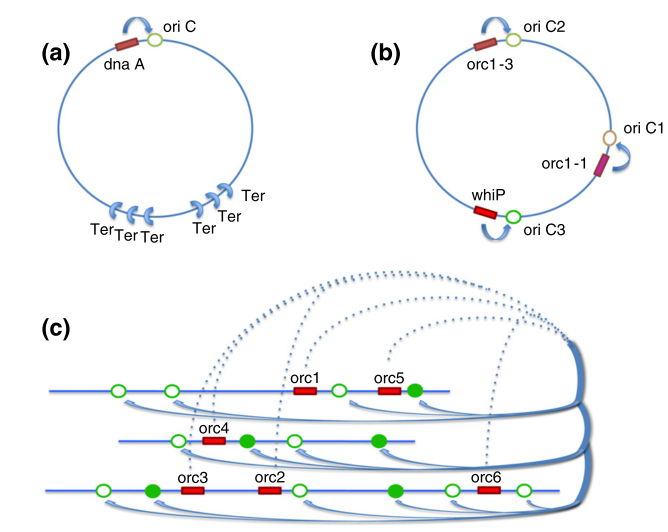
\includegraphics[height=0.4\textheight]{./img/replicon_diversification.png}
	\caption[Diversité des réplicons des trois domaines du vivant]{Diversité des réplicons des trois domaines du vivant. (a) Chromosome bactérien type avec une unique origine de réplication (\textit{ori}) et un site de terminaison à l'opposé. (b) Réplicon de type archée avec plusieurs \textit{ori} inspiré du génome de \textit{Sulfolobus islandicus}. (c) Génome eucaryote typique à multiples origines de réplication ORC. Tiré de \citep{hyrien2013simple}.}\label{figreplintro}
	 \end{center}
 \end{figure} 

	Différents réplicons peuvent être présents sur une même molécule d'ADN, ce qui est le cas général chez les Eucaryotes et semble être fréquent chez Archées \citep{samson2011cell}, cette configuration permettant alors de multiples amorçages de l'initiation de la réplication. Dans ce cas, il n'existe pas de site de terminaison précis. Chez les bactéries par contre, il est communément admis que chaque molécule d'ADN possède un unique réplicon actif.
Dans l'étude du génome d'\textit{Escherichia coli}, un des principaux et premiers organismes modèles en biologie, l'initiation de la réplication du génome, constitué d'un unique chromosome circulaire, s'effectue à un seul site, correspondant à la séquence d'origine de réplication ou \textbf{\textit{ori}} \citep{skarstad1986timing}. Ce phénomène, étant observé chez d'autres espèces bactériennes ainsi que pour des plasmides (voir ci-dessous) \citep{Messer2002,worning2006origin}, le terme ``réplicon" a été généralisé pour désigner, chez les bactéries, les différentes entités génomiques composées d'une unique molécule d'ADN. Quelques exceptions existent toutefois dans le cas des plasmides bactériens. Par exemple, des plasmides tels que les plasmides pGSH500 et pJD4 de \textit{Klebsiella pneumoniae} et \textit{Neisseria gonorrhoeae} respectivement, possèdent plusieurs \textit{ori} (réplicons \textit{sensu stricto}), ce qui leur permet de mieux s'intégrer dans le génome de multiples hôtes \citep{Toukdarian2004}.
 
 
 \subsection{Réplicons essentiels et accessoires}\label{essacc}
Le génome bactérien est constitué de réplicons essentiels à la survie des cellules, les chromosomes, et de réplicons non essentiels, les plasmides \citep{Mackenzie2004}. Historiquement, le terme de "plasmide" a été introduit par Lederberg en 1952 \citep{lederberg1952cell} et désignait à l'époque toute particule extra-chromosomique capable de se reproduire dans un état autonome. Cette définition englobait en fait ce que l'on désigne aujourd'hui sous les termes de ``virus", ``bactériophage", ``ribosome", ``transposon", ``séquence d'insertion" en plus de la définition actuelle de ``plasmide" \citep{lederberg1952cell}. Comment alors définir proprement un plasmide? Par opposition à un chromosome et aux autres éléments extra-chromosomiques, un plasmide peut être caractérisé par son spectre d'hôtes, son mode de réplication plus ou moins autonome vis-à-vis du génome de l'espèce hôte, sa capacité de mobilité inter-hôte, et par des mécanismes d'incompatibilité inter-plasmidique \citep{Slater2008,helinski2004introduction}. Les plasmides diffèrent des chromosomes en présentant des très hauts taux de flux génétiques, et peuvent porter des éléments génétiques provenant de bactéries qui n'ont pas ou peu de caractéristiques en commun. Les plasmides peuvent donc être vus comme des mosaïques de modules fonctionnels aux origines phylogéniques diverses \citep{Fernandez-Lopez2006}.\\
	La notion d'essentialité pour un réplicon est cependant ambiguë, dans le sens où un réplicon peut être qualifié d'essentiel si et seulement si il comporte au moins un gène essentiel à la survie de l'organisme \citep{Mackenzie2004}. Des marqueurs traditionnellement utilisés pour déterminer l'essentialité d'un réplicon sont les gènes codant les ARN ribosomiques (ARNr) \citep{Mackenzie2004}. L'étude de génomes réduits a fourni différents ensembles de gènes considérés comme étant essentiels à la survie des organismes bactériens \citep{Glass2006,Koonin2000}, qui peuvent être, de même, utilisés comme marqueurs d'essentialité de l'élément génétique. Mesurer l'essentialité d'un gène est cependant une tâche ardue en pratique. Elle dépend souvent de l'écologie de l'organisme et peut varier, pour un gène donné, d'un organisme à un autre. Enfin, dans certaines conditions, la perturbation d'un gène peut gravement entraver la capacité d'un organisme à se développer et à prospérer sans forcément le tuer \citep{Mackenzie2004,Slater2008}. Doit-on alors trancher sur le statut ``essentiel" ou ``accessoire" d'un gène donné selon la survie de l'organisme en cas d'altération du géne, ou peut-on plutôt parler de différents degrés d'essentialité d'un gène, et par extension d'un réplicon, selon l'organisme considéré?
 
 
 \subsection{Distribution des réplicons}
Le génome d'\textit{E. coli}, espèce modèle de référence, est composé d'un large réplicon: le chromosome et, selon les souches, de réplicons plasmidiques additionnels plus petits. Ce schéma est largement retrouvé parmi les bactéries. \textbf{La structure typique des génomes bactériens est donc: un unique chromosome, coexistant éventuellement avec des plasmides.} Cette constatation a été largement utilisée afin de décrire les génomes bactériens: le réplicon le plus large étant généralement désigné comme le chromosome et considéré comme essentiel, et les réplicons additionnels étant considérés comme des plasmides, donc accessoires \citep{casjens1998diverse}. Néanmoins, de nombreuses exceptions existent au sein des génomes bactériens (ces éléments seront approfondis dans le Chapitre \ref{chap1b}), ce qui remet en cause ce paradigme. 


\subsection{Taille des réplicons}
	Les réplicons bactériens présentent une très grande diversité de taille. Pour les chromosomes et réplicons extra-chromosomiques dont les séquences complètes étaient disponibles dans la base de données publiques RefSeq à la date du 23 octobre 2013, la taille des chromosomes varie de 139 kb (\textit{Candidatus} Tremblaya princeps (\textit{PCVAL} \citep{lopez2011complete}) à 14.782 kb (\textit{Sorangium cellulosum} \citep{han2013extraordinary}) et de 0,74 kb (\textit{Candidatus} Tremblaya phenacola (\textit{PAVE} \citep{husnik2013horizontal}) à 2.580 kb \textit{Cupriavidus metallidurans} CH34 (NC\_007974.2)) pour les plasmides. Il est intéressant de constater que la taille du plus grand des plasmides est 20 fois plus importante que celle du plus petit des chromosomes: $\frac{\textrm{Taille du plus grand plasmide}}{\textrm{Taille du plus petit chromosome}}\simeq 20$. Même si les distributions de taille sont notablement différentes, elles ne sont pas strictement distinctes.
	
	 
\subsection{Ploïdie/multiplicité des réplicons}
 Les chromosomes bactériens sont souvent perçus comme haploïdes \citep{casjens1998diverse} par opposition aux plasmides qui sont vus comme potentiellement polyploïdes. Même si ces postulats se révèlent souvent corrects, il existe de nombreuses exceptions à cette règle. \textit{Deinococcus radiodurans} \citep{White1999}, \textit{Epulopiscium} sp. \citep{mendell2008extreme}, ou \textit{Neisseria gonorrhoeae} \citep{tobiason2006obligate} présentent une multiplicité de leur chromosome. Il existe de plus une grande variation du nombre de copies possibles d'un plasmide dans une cellule bactérienne \citep{helinski2004introduction}. Pour décrire cette diversité, deux exemples peuvent être cités: les mégaplasmides de la famille des Rhizobiaceae qui, pour certains, sont présents en une unique copie dans l'organisme \citep{Pinto2012} et le plasmide ``modèle" d'\textit{E.coli}, ColE1, qui peut être présent en plus de 20 copies dans une cellule \citep{summers1984multimerization}.
 La régulation du nombre de copies chez les plasmides et chromosomes passe par de nombreux mécanismes génétiques que nous allons aborder dans les sections suivantes.


 \subsection{Topologie des réplicons}
	Même si une configuration circulaire est la norme chez les réplicons plasmidiques et chromosomiques bactériens \citep{casjens1998diverse}, il existe différents exemples de chromosomes \citep{chaconas2005replication} et de plasmides \citep{stewart2004linear} adoptant une configuration linéaire. Par exemple, dans le génome de \textit{Borrelia burgdoferi}, le chromosome de 0,9 Mb et 12 des 22 plasmides présentent une configuration linéaire. Divers réplicons linéaires chromosomiques (de grande taille) et plasmidiques sont aussi trouvés chez les Actinobactéries. Différentes solutions au problème de la terminaison de la réplication des réplicons linéaires coexistent dans le domaine bactérien \citep{hinnebusch1993linear}, suggérant des évolutions multiples indépendantes de cette topologie. Le rôle et les avantages d'une topologie linéaire des réplicons restent cependant flous \citep{casjens1998diverse,chaconas2005replication}. Une apparition secondaire par linéarisation de la forme circulaire est favorisée \citep{volff2000new} et peut être réversible.
 

\subsection{Spectre d'hôte des plasmides}\label{spectrehote}
	Les plasmides sont différenciés selon leur capacité à exister dans divers hôtes bactériens. On distingue alors les plasmides à spectre d'hôtes étroit ou large selon le nombre d'hôtes qui peuvent les héberger. Cette propriété est principalement en rapport avec une adaptation particulière des mécanismes de la réplication, ségrégation et maintenance plasmidiques \citep{Toukdarian2004,jain2013broad}. 
 

\subsection{Rôle des plasmides} 
	À travers les différents aspects abordés, aucune distinction majeure entre chromosomes et plasmides n'apparaît, hormis un aspect essentiel ou accessoire des réplicons. Néanmoins, les chromosomes, en tant que partie essentielle du génome bactérien, \textit{définissent} leur hôte. Ainsi, toute spécificité génomique de ceux-ci reflétera l'adaptation de l'organisme bactérien à son écologie et à son mode d'évolution \citep{bentley2004comparative}. Inversement, les éléments plasmidiques peuvent présenter un caractère ``égoïste" par l'évolution de stratégies permettant leur existence propre sans forcément apporter une contribution significative aux organismes hôtes \citep{Lili2010,thomas2004}. Cet aspect est souvent nuancé par différents auteurs arguant qu'un comportement purement égoïste d'un plasmide, se maintenant au fil des générations par simple réplication, maintenance et transfert, ne semble pas viable sur le long terme d'un point de vue évolutif \citep{thomas2004,Slater2008}. Diverses stratégies ont été adoptées par les plasmides en diminuant leurs éventuels effets négatifs sur la croissance de l'hôte et/ou en contribuant à lui apporter un avantage évolutif significatif \citep{de2007gene,Heuer2008}. Celles-ci incluent des adaptations de leurs mécanismes de réplication, ségrégation, d'incompatibilité, de maintenance, d'addiction génétique et de transfert afin d'optimiser leur stabilisation au sein du génome-hôte et leur transmission inter-génomique. Il existe de nombreux exemples où les plasmides contribuent fortement à l'adaptation de l'organisme bactérien hôte à son environnement en étant, par exemple, porteur de gènes de virulence ou de résistance à des composés tels que les antibiotiques. Enfin, en tant que particule extra-chromosomique auto-réplicative, chaque plasmide possède une dynamique de population spécifique qui dépend de ces mécanismes génomiques et de l'écologie de l'organisme dans lequel celui-ci est présent \citep{Slater2008}.
 

\section{Architecture des réplicons: mécanismes structuraux}\label{spatial}
	Il a longtemps été estimé que le nucléoïde bactérien était un amas compact d'ADN sans structure. Les chromosomes bactériens sont en fait organisés en plusieurs super-enroulements alignés tels les perles d'un collier, cette structure dépendant de divers complexes protéiques et de petites molécules associées au nucléoïde \citep{thanbichler2010}. Les chromosomes bactériens sont orientés selon leur origine de réplication et le site de terminaison de la réplication, mais également en fonction de leur centromère \textit{parS} (séquence de fixation des protéines ségrégatives). Ils possèdent de plus une orientation spatiale spécifique, les positionnements de leurs origine de réplication et site de terminaison dans la cellule dépendant rigoureusement du cycle cellulaire \citep{Toro2010}.\\

	
\subsection{Nucleoid-associated proteins}  
	Les \textit{\textbf{N}ucleoid \textbf{A}ssociated \textbf{P}roteins} (NAP) sont une classe de protéines se fixant à l'ADN et intervenant dans la structure spatiale du génome \citep{Dillon2010}. En agissant au niveau de la structure de l'ADN, ces molécules ont de plus un rôle régulateur de fonctions telles que la réplication, la recombinaison et la maintenance, mais aussi de la réparation et de la transcription de l'ADN \citep{azam1999twelve}. Les principales NAP sont décrites Table \ref{tabnap} et leur propriétés des mieux connues sont présentées Table \ref{tabnap2}. Parmi les NAP majoritairement isolées d'\textit{E. coli} HU, IHF, H-NS, StpA et Fis sont les plus abondantes \citep{Johnson2005a}. CbpA, CbpB (aussi connue sous le nom de Rob) et Lrp sont représentées de façon plus minoritaire parmi les bactéries \citep{Johnson2005a}. 
	  
\begin{longtable}{@{\hspace{-2cm}\hspace{1cm}} >{\bfseries}p{0.1\textwidth} | >{\small}p{\textwidth}}
	\caption{Principales protéines s'associant au nucléoïde (NAP)}
	\label{tabnap}\\
	\endfirsthead
	HU & (\textbf{H}eat \textbf{U}nstable) est une protéine de type histone. Elle semble impliquée dans la compaction de l'ADN et est présente chez la plupart des bactéries. Des homologues HU semblent exister chez les Eucaryotes et Archées. HU est de plus impliquée dans la réplication, la ségrégation et la division cellulaire, en permettant notamment la stabilisation de la protéine DnaA sur \textit{ori}. HU intéragit avec les superenroulements de l'ADN de façon non-spécifique, avec l'ADN simple brin ainsi qu'avec l'ARN \citep{Johnson2005a}.\\
	\\[-0.2cm]
	IHF & (\textbf{I}ntegration \textbf{H}ost \textbf{F}actor) est un paralogue de HU et, de même, est en lien avec la condensation de l'ADN ainsi qu'avec la réplication, la ségrégation et la division cellulaire \citep{Johnson2005a}. IHF reconnaît spécifiquement des séquences de 30 à 35 paires de bases (pb). Elle est trouvée chez différentes espèces de Protéobactérie (bactéries Gram-négatif) mais n'est pas décrite chez les bactéries Gram-positif. IHF semble intervenir avec Fis (\textit{cf.} ci-après) au niveau d'\textit{ori} et joue un rôle dans la régulation de l'initiation de la réplication \citep{Johnson2005a}.\\
	\\[-0.2cm]
	H-NS & (\textbf{H}istone-like \textbf{N}ucleoid \textbf{S}tructuring protein) est une protéine structurale s'attachant de façon non-spécifique préférentiellement sur des régions riches en A+T, retrouvée chez de nombreuses bactéries Gram-négatif. H-NS contraint les superenroulements \textit{in vitro} et influence la structure de l'ADN localement \citep{Johnson2005a}. C'est un homologue de StpA (\textit{cf.} ci-dessous).\\
	\\[-0.2cm]
	Fis & (\textbf{F}actor for \textbf{i}nversion \textbf{s}timulation) est une protéine structurale jouant différents rôles de régulation (de nombreuses fonctions telles que la réplication et la ségrégation) en s'attachant à des centaines de sites sur l'ADN d'\textit{E. coli} \citep{Browning2010}. Fis est capable de ``tendre" l'ADN et, ainsi, de promouvoir ou d'inactiver différents promoteurs \citep{Dillon2010}.\\
	\\[-0.2cm]
	Lrp & (\textbf{L}eucine-responsive \textbf{r}egulatory \textbf{p}rotein) influence la transcription de 10\% des gènes d'\textit{E. coli} en agissant soit comme activateur, soit comme répresseur. En plus d'intervenir dans la régulation des gènes impliqués dans le métabolisme, la virulence ou l'expression du pilus, Lrp influence la structure du nucléoïde \citep{Browning2010}. Son implication dans le cycle cellulaire d'\textit{E. coli} a été démontré \citep{corcoran2009dna}. Des homologues de Lrp tels que AsnC ou PutR (révélés par des analyses de similarité de séquences avec HMMER; \textit{cf.} Chapitre \ref{chap3b}) sont retrouvés chez l'ensemble des bactéries.\\
	\\[-0.2cm]
	CbpA & (\textbf{C}urved-DNA \textbf{b}inding \textbf{p}rotein textbf{A}) est un homologue de la protéine DnaJ. CbpA a la capacité de se fixer à l'ADN et est liée au  cycle cellulaire. Elle contribue à la croissance à basse température des bactéries et est nécessaire pour un déroulement normal de la division cellulaire. CbpA est décrite chez de nombreuses bactéries \citep{Dillon2010}.\\
	\\[-0.2cm]
	CbpB & (\textbf{C}urved-DNA \textbf{b}inding \textbf{p}rotein \textbf{B}) ou \textbf{Rob} (\textbf{R}ight \textbf{o}rigin \textbf{b}inding) est une protéine se liant à l'ADN au niveau de sites d'attache localisés à proximité de l'\textit{ori} et de différents promoteurs (dont celui de son gène) et semble de ce fait être un facteur de transcription \citep{azam1999twelve}.\\ 
	\\[-0.2cm]
	Dps & (\textbf{D}NA \textbf{p}rotection during \textbf{s}tarvation protein) est une protéine du cycle cellulaire qui, chez \textit{E. coli}, contribue au compactage de l'ADN et au passage de la phase exponentielle de croissance à la phase stationnaire \citep{azam1999twelve}.\\
	\\[-0.2cm]
	StpA & (\textbf{S}uppressor of \textbf{t}d mutant \textbf{p}rotein \textbf{A}) est un homologue de séquence de H-NS et est de même capable de courber la molécule d'ADN \citep{azam1999twelve}. StpA peut former un hétéro-complexe avec H-NS et possède différentes activités régulatrices, notamment au niveau de la croissance cellulaire \citep{Dillon2010}.\\
\end{longtable}
\begin{table}[H]
	\hspace{-1.5cm}
	\caption[Propriétés des NAP majoritaires des bactéries]{Propriétés des NAP majoritaires des bactéries.}\label{tabnap2}
	\small 
	\begin{tabular}[left]{lcccp{0.45\textwidth}cp{0.15\textwidth}}
	\multicolumn{6}{l}{\textbf{Bactéries Gram négatif}}\\
	\textbf{P}$^{a}$ & \textbf{C}$^{b}$ & \textbf{P}$^{c}$ & \textbf{T}$^{d}$ & \textbf{Motif} & \textbf{M}$^{e}$ & \textbf{Pr}$^{f}$\\
	\hline
	HU & oui & ND & oui & joint à l'ADN db ou sb; préférence pour les zones riches en A+T & $\sim9kDa$ & hétérodimère ($HU\alpha-HU\beta$)\\
	\\[-0.2cm]
	IHF & ND & ND & Oui & (A/T=ATCAANNNNTT(A/G) & $\sim11kDa$ & hétérodimère ($IHF\alpha-IHF\beta$\\
	\\[-0.2cm]
	H-NS & ND & Oui & ND & zone riche en A+T et TCGATAAATT & $\sim15kDa$ & homodimère ou hétérodimère (H-NS-StpA)\\
	\\[-0.2cm]
	Fis & Oui & Oui & Oui & zones riches en A ou A+T & $\sim11kDa$ & homodimère\\
	\\[-0.2cm]
	Lrp & Oui & Oui & ND & (T/C)AG(A/T/C)A(A/T)ATT(A/T)T(A/T/G) & $\sim18kDa$ & homodimère\\
	\\[-0.2cm]
	CbpA & ND & ND & ND & ADN courbé & $\sim33kDa$ & monomère\\
	\\[-0.2cm]
	Dps & ND & ND & ND & ND & $\sim19kDa$ & monomère ou dodécamère\\
	\\[-0.2cm]
	StpA & ND & Oui & ND & zone riche en A+T & $\sim15kDa$ & homodimère ou hétérodimère ($StpA-H-NS$)\\
	\\[-0.2cm]
	MukB & ND & Oui & ND & ND & $\sim175kDa$ & homodimère\\
	\\[-0.4cm]
	\multicolumn{6}{l}{\textbf{Bactéries Gram positif}}\\
	\textbf{P}$^{a}$ & \textbf{C}$^{b}$ & \textbf{P}$^{c}$ & \textbf{T}$^{d}$ & \textbf{Motif} & \textbf{M}$^{e}$ & \textbf{Pr}$^{f}$\\
	\hline
	\\[-0.2cm]
	HU & ND & ND & Oui & ND & $\sim10kDa$ & homodimère\\
	Lrp & Oui & Oui & ND & ND & $\sim17kDa$ & homodimère\\
	MukB & ND & Oui & ND & préférence pour ADNsb & $\sim130kDa$ & homodimère\\
	\end{tabular}
	\captionsetup{labelsep=space,justification=justified,singlelinecheck=off}
	\caption*{\footnotesize $^{a}$ P: nom de la NAP. \\  $^{b}$ C: capacité de la protéine à condenser l'ADN au niveau du motif de fixation.\\ $^{c}$ P: capacité de la protéine à faire des ``ponts" au niveau du motif de fixation.\\ $^{d}$ T: capacité de la protéine à tendre l'ADN au niveau du motif de fixation\\ $^{e}$ M: masse moléculaire en kiloDalton. \\ $^{f}$ Pr: promoteur natif.\\ Adapté de \citep{Dillon2010}.}
\end{table}
\captionsetup{}

	Ces protéines, étant liées à la structure du nucléoïde, interviennent sur la transcription d'une manière globale. Les effets sur la transcription ne proviennent pas uniquement des changements du nombre de protéines disponibles au cours des différentes étapes du cycle cellulaire mais dépendent aussi du passage de la fourche de réplication \citep{Browning2010}. Il existe de plus de nombreuses preuves d'interaction et de régulation entre les NAP aux niveaux géniques et protéiques. Par exemple, il existe une régulation croisée entre IHF, Fis et H-NS au niveau du promoteur de \textit{dps}. H-NS inhibe les promoteurs de \textit{stpA}. \textit{hns} est lui même sous le contrôle de Fis. Lrp auto-régule négativement son propre gène et active \textit{stpA} \citep{Dillon2010}. Enfin, il est à noter qu'il existe une interaction entre IHF et le super-régulateur CtrA (chez les alphaprotéobactéries) régulant l'initiation de la réplication en changeant l'architecture d'\textit{ori}\citep{thanbichler2010}.



\subsection{Motifs structurels du nucleoïde}\label{motifstruc}
  La régulation des mécanismes du cycle cellulaire implique dans presque tous les cas connus des intéractions entre éléments \textit{cis} (séquences d'ADN) et \textit{trans} (éléments diffusibles: protéines ou ARN régulateurs). Le cycle cellulaire est donc en quelque sorte reflété dans la séquence du nucléoïde. Les motifs, courtes séquences caractéristiques d'ADN, sont des cibles privilégiées des facteurs de transcription et de structure (\textit{i.e.}, les NAP). Un inventaire non-exhaustif des principaux motifs impliqués dans la réplication, la ségrégation et la maintenance du chromosome bactérien \citep{Touzain2011} est présenté Tables \ref{tabmotif} et \ref{tabmotif2}.
	
\begin{longtable}{@{\hspace{-2cm}\hspace{1cm}} >{\bfseries}p{0.2\textwidth}  | >{\small}p{0.9\textwidth}}
 	 \caption{Motifs structurels du nucleoïde}\label{tabmotif}\\
	 \endfirsthead
	 Boîtes DnaA & Ces motifs sont impliqués dans le contrôle de l'initiation de la réplication en permettant la stabilisation de la protéine initiatrice DnaA (\textit{cf.} ci-après). Ces motifs (comme DnaA) sont conservés parmi les bactéries. Ils sont présents à l'\textit{ori} du chromosome ainsi que sur des sites secondaires impliqués dans la séquestration de DnaA. Il existe différents types de boîtes DnaA sur lesquelles se fixent DnaA avec plus ou moins d'affinité selon sa conformation \citep{Mott2007}.\\
	\\[-0.2cm]
	\textit{chi} & Ces motifs (octamériques chez \textit{E. coli}) interagissent avec les recombinases homologues RecBCD qui interviennent dans la réparation de l'ADN. Ces sites sont orientés et permettent de ``guider" les recombinases \citep{spies2005homologous}. Ces sites sont très conservés dans toutes les espèces examinées \citep{Touzain2011}.\\
	\\[-0.2cm]
	\textit{dif} & Ce site, localisé à proximité du site de l'arrêt de la réplication des chromosomes bactériens, permet la fixation et l'action des systèmes de résolution de dimère de réplicon (systèmes Xer). Ces sites de type palindrome sont très conservés parmi les chromosomes bactériens et sont aussi trouvés chez les Archées \citep{Carnoy2009}. \\
	\\[-0.2cm]
	 GATC & Ces motifs de quatre nucléotides interagissent principalement avec Dam et SeqA, deux protéines impliquées dans l'initiation de la réplication ainsi que MutH. Selon leur état méthylé ou non, ils interviennent dans l'identification du brin ADN néo-formé dans les processus de réplication et de réparation de l'ADN. Ils semblent également avoir un rôle dans la ségrégation des chromosomes et sont des séquence cis-régulatrices de gènes. Ces motifs sont stratégiquement localisés par rapport à l'\textit{ori}. La reconnaissance des GATC par Dam semble cependant être limitée aux gamma-protéobactéries \citep{Touzain2011}.\\
	\\[-0.2cm]
	KOPS & (Fts\textbf{K}-\textbf{O}rienting\textbf{ P}olar \textbf{S}equences) Ces motifs orientés dans le sens de la réplication et donc inversés au site de terminaison de la réplication\citep{Kono2011}, guident les processus de résolution de dimère au site \textit{dif} \citep{bigot2005kops}. Ils interviennent dans le guidage des recombinases site-spécifiques XerCD, responsables de la résolution de dimère de chromosomes au site \textit{dif} avec la protéine FtsK, elle-même guidée par les motifs KOPS qui permettent sa fixation selon une orientation donnée. \\
	\\[-0.2cm]
	 NBS & (\textbf{N}oc-\textbf{B}inding \textbf{S}ites). Ces motifs de 14 pb chez \textit{B. subtilis} sont les sites de fixation de la protéine Noc (Nucleoid occlusion protein) qui protège le chromosome d'une section par une mauvaise position du septum. Ils sont impliqués dans la prévention de l'assemblage de l'appareil moléculaire lié à la division cellulaire. SlmA est un analogue de Noc chez \textit{E. coli} mais présente une séquence différente. Il est donc probable que, tout comme Noc, SlmA se fixe sur des sites particuliers.\\
	\\[-0.2cm]
	\textit{oriT} & Site de coupure des relaxases sur les éléments conjugatifs (voir \ref{conj}). Ces sites peuvent être classés en différents groupes. Un même groupe peut rassembler des sites provenant de plasmides de bactéries Gram-négatif ou Gram-positif, ce qui suggère une origine commune à la conjugaison des éléments génétiques \citep{lawley2004bacterial}.\\
	\\[-0.2cm]
	\textit{parS} & Ce site est l'homologue bactérien du centromère. Il stimule la ségrégation des chromosomes néo-formés par l'interaction avec ParA et ParB, des analogues du cytosquelette eucaryotique \citep{Livny2007}. Les motifs \textit{parS} sont des palindromes de 16 pb (chez \textit{Bacillus subtilis}) et sont situés, en un ou deux exemplaires, à proximité de l'\textit{ori}. Ceux-ci, tout comme le système ParA/ParB, sont très conservés dans le domaine bactérien à l'exception de certaines gamma-protéobactéries (Enterobactéries, dont \textit{E. coli}) qui, elles, utilisent similairement le site \textit{migS} \citep{Livny2007,Mierzejewska2012}.\\
	\\[-0.2cm]
	 \textit{ram} & (\textbf{Ra}cA binding \textbf{m}otifs) Ces sites sont impliqués dans l'accrochage de l'\textit{ori} aux pôles de la cellule \textit{via} RacA lors de la sporulation chez \textit{B. subtilis}.\\
	\\[-0.2cm]
	 \textit{ter} & (pour terminaison) Ces sites font 23 pb de long et sont localisés dans la région opposée à l'\textit{ori}. Ils sont impliqués dans la terminaison de la réplication. Chez \textit{E. coli}, ce sont les sites de fixation de la protéine Tus qui intervient dans la déstabilisation des fourches de réplication et l'arrêt de la réplication. Ils sont faiblement conservés parmi les génomes bactériens.\\
	\end{longtable}

\begin{table}[H]
	\footnotesize
	\hspace{-2.5cm}
	\caption[Caractéristiques des principaux motifs trouvés chez les bactéries]{Caractéristiques des principaux motifs trouvés chez les bactéries. Adapté de \citep{Touzain2011}.}
	\label{tabmotif2}
	\begin{tabular}{p{0.15\textwidth}|>{\scriptsize}p{0.35\textwidth}p{0.15\textwidth}|p{0.15\textwidth}p{0.15\textwidth}}
	\textbf{Nom} & \textbf{\footnotesize Consensus} & \textbf{Nombre} & \textbf{Protéine} & \textbf{Fonction}\\
	\hline
	\multirow{2}{0.15\textwidth}{Boîte DnaA} & TTATNCACA (\textit{E. coli}) & 107 & DnaA & \multirow{2}{0.2\textwidth}{Initiation de la réplication}\\
	\cline{2-3}
	 & TTATNCACA (\textit{B. subtilis}) & 211\\
	\hline
	GATC & GATC (\textit{E. coli}) & 19.120 & Dam, SeqA, MutH & Identification du brin néo-synthétisé\\
	\hline
	\multirow{2}{0.15\textwidth}{\textit{ter}} & GN(A/G)NGTTGTAA(C/T)(T/G)A (\textit{E. coli}) & 10 & Tus ou Rtp & \multirow{2}{0.2\textwidth}{Terminaison de la réplication}\\
	\cline{2-3}
	 & (G/T)(A/C)ACT(A/G)AN (A/T)(A/G)(A/C/T)(A/T) (T/C)(T/A)(A/G)T et (T/A)(A/G)TG(T/A)AC(C/T) AAAT(G/A/T)TT(C/T) (\textit{B. subtilis}) & 7-8 & \\
	\hline
	\multirow{5}{0.15\textwidth}{Chi} & GCTGGTGG (\textit{E. coli}) & 1.008 & \multirow{5}{0.15\textwidth}{RecBCD ou AddAB} & \multirow{5}{0.2\textwidth}{Réparation des cassures double-brin}\\
	\cline{2-3}
	 & GNTGGWGG (\textit{Haemophilus influenzae}) & 408\\
	\cline{2-3}
 	& AGCGG (\textit{B. subtilis}) & 11.381\\
	\cline{2-3}
 	& GAAGGGG (\textit{Staphylococcus aureus}) & 339\\
	\cline{2-3}
 	& GCGCGTG (\textit{Lactococcus lactis} & 187\\
	\hline
	\textit{parS} & (T/C)GTT(T/A/C)CA(C/T)(G/A) TG(A/G/T)AAC(A/G) (\textit{B. subtilis}) & 10 & SpoOJ & Ségrégation d'\textit{ori}\\
	\hline
	\textit{migS} & ATTTTTGCGGGTACTCAGCAAAATT (\textit{E. coli}) & 1 & Inconnue & Ségrégation d'\textit{ori}\\
	\hline
	ram & TGNCGCCGGCGNCA (\textit{B. subtilis}) & 923 & RacA & Ségrégation d'\textit{ori} durant la sporulation\\
	\hline
	KOPS ou SRS & GGGNAGGG (\textit{E. coli}) & 366 & FtsK & Ségrégation du chromosome
	\end{tabular}
	\label{tabmotif2}
\end{table}
			
		
\subsubsection{NAP et motifs structurels chez les plasmides}\label{motif}
	Tout comme les chromosomes, les plasmides possèdent une structure dont une partie est contrainte et maintenue par différents mécanismes \citep{higgins2004topological}. Le spectre d'hôtes des plasmides est lié à leurs interactions avec les protéines structurales des hôtes (notamment IHF et Fis) \citep{DelSolar1996,Toukdarian2004}. De nombreux NAP et les mécanismes impliqués dans la structure et la régulation des chromosomes ont donc également un rôle dans la structure des plasmides. Par exemple, IciA, Fis, IHF, HU interviennent dans la régulation de l'initiation de la réplication de certains plasmides \citep{Kruger2004,DelSolar1998}. Fis se fixe à certains plasmides \citep{Rimsky2011} et différents plasmides transmissibles codent pour un homologue de H-NS \citep{Browning2010}. Des boîtes DnaA ont été identifiées au niveau de l'\textit{ori} de différents plasmides (\textit{cf.} \ref{ori}) et des homologies de séquence existent entre les séquences centromériques plasmidiques et chromosomiques \citep{Livny2007,Mierzejewska2012}. Les plasmides semblent cependant posséder certaines spécificités structurales, telles que des origines de réplication organisées en itérons (motifs spécifiques permettant l'attachement des protéines initiatrices Rep) et des homologues des NAP chromosomiques et/ou de motifs structurels spécifiques.    


\section{Réplication des réplicons}
	La réplication chez les Eucaryotes, Archées et Bactéries présentent des similitudes: elle débute avec la fixation au niveau d'une région spécifique de l'ADN (origine) de la protéine initiatrice, ce qui provoque l'ouverture de la molécule double-brin et l'établissement d'un complexe de réplication. La réplication des chromosomes doit s'effectuer une seule fois durant le cycle cellulaire sous peine de létalité pour la cellule. La réplication est suivie d'une phase de ségrégation du matériel génomique néo-formé et de partition dans les deux cellules filles, chacune récupérant un complément génomique  (Figure \ref{figRepl}). Ces étapes sont sous le contrôle de différents mécanismes de maintenance coordonnant leurs déclenchement et inhibition en rapport avec le cycle cellulaire \citep{thanbichler2010,OSullivan2011}. La duplication des plasmides suit les mêmes processus, ceux-ci pouvant cependant posséder des mécanismes de régulation spécifiques.
	
\begin{figure}[H]
	\begin{center}
		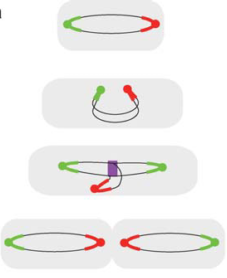
\includegraphics[scale=0.8]{./img/repl_simple.png}
	\end{center}
 \caption[Représentation schématique de la réplication du chromosome bactérien]{Représentation schématique de la réplication du chromosome bactérien. \\ Vert: \textit{ori}. Rouge: sites de terminaison. Violet: réplisome. Adapté de \citep{Ghosh2006}} \label{figRepl}
 \end{figure}
 
Dans la réplication de tout réplicon, trois phases peuvent être distinguées: 
\begin{description}
\item[$\bullet$] L'initiation qui correspond à l'ouverture de l'\textit{ori} par des protéines initiatrices.
\item[$\bullet$] L'élongation ou assemblage du brin néo-formé par les ADN-polymérases.
\item[$\bullet$] La terminaison qui est la relaxation des complexes de réplication pouvant s'accompagner de la résolution de dimère.
\end{description}
La réplication chez les chromosomes bactériens est conservée et suit globalement le modèle décrit chez \textit{E. coli}, alors qu'il existe trois types de réplication dans le cas des plasmides \citep{DelSolar1998}:
\begin{description}
\item[$\bullet$] la réplication thêta, similaire à la réplication chromosomique,
\item[$\bullet$] la réplication par rotation de cercle (RC),
\item[$\bullet$] la réplication par déplacement de brin (SD).
\end{description}
Parmi les plasmides à réplication de type thêta, on peut différencier les plasmides à itérons, sites spécifiques d'interaction avec les protéines Rep au niveau de leur \textit{ori}, et les plasmides de type ``DnaA-like" \citep{petersen2011origin}, des autres plasmides. \\
Les mécanismes et protéines majeurs impliqués dans la réplication, la ségrégation et le cycle cellulaire du génome bactérien sont résumés ci-dessous. La littérature existante fait majoritairement référence à quelques organismes modèles seulement, les principaux étant \textit{E. coli} (gamma-protéobactérie), \textit{Caulobacter crescentus} (alpha-protéobactérie) et \textit{Bacillus subtilis} (firmicute).\\


 \subsection{Origine et initiation de la réplication}\label{ori}
	Toutes les cellules des trois domaines de la vie possèdent des mécanismes de régulation contrôlant la réplication durant la phase d'initiation \citep{clark1967dna}. Les protéines majeures impliquées dans l'initiation de la réplication des réplicons sont présentées Table \ref{taboriini}. Sont ensuite détaillés la structure des origines de réplication, le déroulement et la régulation de l'initiation.
  
 \begin{longtable}{@{\hspace{-2cm}\hspace{1cm}} >{\bfseries}p{0.2\textwidth} | >{\small}p{0.9\textwidth}}
	 \caption{Principales protéines impliquées dans l'initiation de la réplication}
	 \label{taboriini}\\
	 \endfirsthead
	 DnaA & protéine s'attachant à l'ADN de façon spécifique. C'est un acteur principal de la cascade d'événements initiant la réplication des chromosomes bactériens et de certains plasmides \citep{petersen2011origin}. Ces événements incluent la reconnaissance de l'origine (\textit{ori}), son ouverture et l'attachement d'hélicases \citep{higgins2005bacterial}. DnaA est aussi un facteur de transcription \citep{Messer2002}. On estime que des homologues de DnaA existent chez toutes les espèces bactériennes \citep{yoshikawa1991structure,Messer2002}. \\
	\\[-0.2cm]
	DnaB & l'hélicase réplicative chez les bactéries. Elle est composée de six sous-unités et catalyse la séparation des brins de l'ADN \citep{o2013principles}. De même que pour DnaA, on considère que chaque organisme bactérien dispose d'une hélicase réplicative. Elle est de plus retrouvée dans les trois domaines du vivant.\\
	\\[-0.2cm]
	DnaC & paralogue de DnaA. C'est un facteur supplémentaire permettant l'attachement et la stabilisation de DnaB à \textit{ori} \citep{Mott2007}.\\
	\\[-0.2cm]
	IciA & (\textbf{Inhibitor} of \textbf{c}hromosome \textbf{i}nitiation) membre de la famille des facteurs de transcription LysR, très répandu chez les bactéries Gram négatif. IciA agit en tant qu'antagoniste de DnaA en inhibant l'initiation de la réplication au niveau d'\textit{ori} \citep{Dillon2010}.\\
	\\[-0.2cm]
	Rep & Cette dénomination fait référence de façon générique aux protéines impliquées dans l'initiation de la réplication des plasmides. Elles sont apparentées par leur séquence aux protéines impliquées dans la conjugaison (Tra et Mob) \citep{DelSolar1998} et sont retrouvées sur la plupart des plasmides dont la séquence complète a été réalisée. Elles peuvent comporter des domaines fonctionnels similaires \citep{DelSolar1998}, suggérant une origine commune. Tout comme DnaA avec le chromosome, les protéines Rep intéragissent avec les \textit{ori} plasmidiques par la reconnaissance de motifs spécifiques. La désignation “Rep” englobe les protéines initiatrices nécessaires pour les trois types de réplication plasmidique bien qu'elles puissent correspondre à des protéines différentes avec des fonctions distinctes. Généralement les plasmides de type thêta codent pour un seul initiateur protéique, RepA, TrfA ou RepE, qui active ou inhibe la réplication selon sa configuration (dimère ou monomère) \citep{Kruger2004}. Les plasmides de type SD codent pour trois protéines Rep: RepA (hélicase), RepB (primase) et RepC (facteur stabilisateur de l'hélicase de type DnaC) \citep{DelSolar1998}. Les Rep des plasmides de type RC sont très conservées, et contiennent deux domaines spécifiques: le domaine \textit{dso} de reconnaissance de l'origine et le domaine de coupure  \citep{khan2005plasmid}. Ces protéines possèdent un résidu tyrosine qui est impliqué dans la coupure de l'ADN \citep{khan2005plasmid}. Elles recrutent une hélicase de l'hôte, PcrA, qui possède des homologies avec l'hélicase Rep d'\textit{E. coli}.\\
	\\[-0.2cm]
	 DnaG & primase qui synthétise de courts fragments d'ARN, ou brins d'Okazaki, servant de points d'initiation pour la synthèse d'ADN \citep{o2013principles}.\\
	\\[-0.2cm]
	 Dam & (\textbf{D}NA \textbf{a}denine \textbf{m}ethylase) méthyle les motifs GATC au niveau de l'adénine et participe à la régulation de l'initiation.\\
	\\[-0.2cm]
	 SeqA & (\textbf{Seq}uestration \textbf{A} protein) régule l'initiation de la réplication en se fixant aux motifs GATC hémiméthylés au niveau d'\textit{ori}. L'origine néo-formée est ainsi séquestrée, empêchant un nouvel amorçage de la réplication par DnaA.\\
	\\[-0.2cm]
	 Hda & Homologue de DnaA. Elle intervient dans la régulation de DnaA chez \textit{E. coli}. Elle interagit avec l'ADN polymérase III, ce qui stimule l'activité de DnaA et contribue à l'ouverture de l'ADN au niveau d'\textit{ori}. Des orthologues de Hda ont été trouvés uniquement chez les gamma-protéobactéries \citep{zakrzewska2007regulation}. Chez \textit{B. subtilis}, c'est la protéine YabA qui joue ce rôle \citep{Mott2007}. \\
	\\[-0.2cm]
	 SSB & (\textbf{S}ingle \textbf{S}trand \textbf{B}inding proteins) En se fixant sur l'ADN mono-brin généré par l'ouverture de l'\textit{ori}, ces protéines stabilisent le complexe d'initiation \citep{o2013principles}.\\
	\\[-0.2cm]
	 DiaA & (\textbf{D}NA \textbf{i}nitiator-\textbf{a}ssociating factor) protéine découverte relativement récemment chez \textit{E. coli}. Elle se fixe à DnaA et est impliquée dans la synchronisation de l'initiation \citep{Katayama2010}. \\
	\\[-0.2cm]
	 CtrA & (\textbf{C}ell cycle \textbf{t}ranscriptional \textbf{r}egulator A) régulateur maître, caractérisé chez \textit{C. crescentus}. CtrA contrôle de nombreuses fonctions du cycle cellulaire et agit notamment sur les gènes \textit{ftsZ, ftsA} et \textit{ftsQ} (\textit{cf.} ci-après). Des homologues de CtrA semblent présents uniquement chez les alpha-protéobactéries \citep{Brilli2010,thanbichler2010}. \\
	\\[-0.2cm]
	 DivK & (cell \textbf{div}ision response regulator \textbf{K}) régulateur antagoniste de CtrA lorsque il est activé \citep{Brilli2010}.\\
	\\[-0.2cm]
	 YabA & inhibiteur de DnaA chez \textit{B. subtilis}. YabA forme un complexe avec DnaA et l'ADN polymerase III (\textit{cf.} ci-après) et limite le nombre de protéines initiatrices disponibles \citep{Katayama2010}. YabA est retrouvée chez d'autres bactéries Gram-positif \citep{Mott2007}.\\
	\\[-0.2cm]
	 SirA et Spo0A & (\textbf{S}porulation \textbf{i}nhibitor of \textbf{r}eplication protein \textbf{A} et \textbf{S}porulation stage  \textbf{0} protein \textbf{A}, respectivement) protéines impliquées dans la séquestration d'\textit{ori} chez \textit{B. subtilis} et ses proches voisins taxonomiques seulement.\\
	\end{longtable}
	
	
\subsubsection{Structure des origines de réplication}\label{oristruct}
\begin{description}
\item[$\blacktriangleright$] L'origine de réplication d'un chromosome bactérien typique est une courte séquence nucléotidique (250 pb chez \textit{E.coli}; Figure \ref{figoriecoli}), organisée en une région riche en Adénine et Thymine et en différents motifs structuraux \citep{Robinson2005,rajewska2012rich}.
\begin{figure}[H]
	\begin{center}
		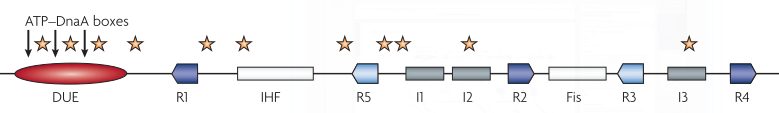
\includegraphics[width=0.9\linewidth]{./img/ori_schema.png}
	\caption[Structure de l'origine de réplication de \textit{E. coli}]{Origine de réplication de \textit{E. coli}.\\ DUE: DNA Unwinding Element, riche en bases A+T. R1, R2, R3, R4: boîtes DnaA orientées. Motifs présentant une affinité forte pour DnaA : bleu sombre, et faible: bleu clair. Rectangles blancs: sites de fixation de IHF et Fis. Étoiles: motifs GATC. Rectangles gris: sites I de fixation préférentielle de DnaA-ATP. Flèches: quatrième classe de motifs de fixation de DnaA-ATP exclusivement, dans DUE. Adapté de \citep{Mott2007}}\label{figoriecoli}.
	\end{center}
\end{figure} 
Sa proximité avec certains gènes engendre plusieurs systèmes de régulation. La plus importante interaction est avec DnaA, au niveau des boîtes DnaA qui structurent l'origine de réplication par leur type et leur orientation et permettent l'ouverture d'\textit{ori} au cours d'un changement de conformation lors de la fixation de DnaA \citep{Mott2007}. La région riche en bases A et T (DNA Unwinding Element; DUE) est le site d'ouverture proprement dit. Relativement moins d'énergie sera nécessaire à son ouverture de par sa richesse en paires A-T (2 liaisons covalentes) en comparaison à une région d'ADN comprenant des appariements G-C (3 liaisons covalentes). Cette région contient de plus, sur le chromosome d'\textit{E. coli}, trois 13-mères caractéristiques organisés en tandem, impliqués dans l'activité de DnaA \citep{Mott2007}. D'autres motifs structurels de cette région participent à la régulation de l'initiation, tels que les motifs d'attache de Fis et IHF et les motifs GATC. L'organisation des \textit{ori} des chromosomes d'autres bactéries présentent de nombreuses similarités avec l'\textit{ori} d'\textit{E.coli} et respectent la structure DUE + motifs spécifiques (boîtes DnaA, site de méthylation de Dam, etc) (Figure \ref{ori_div}). 
\end{description}

\begin{figure}[H]
		\begin{center}
			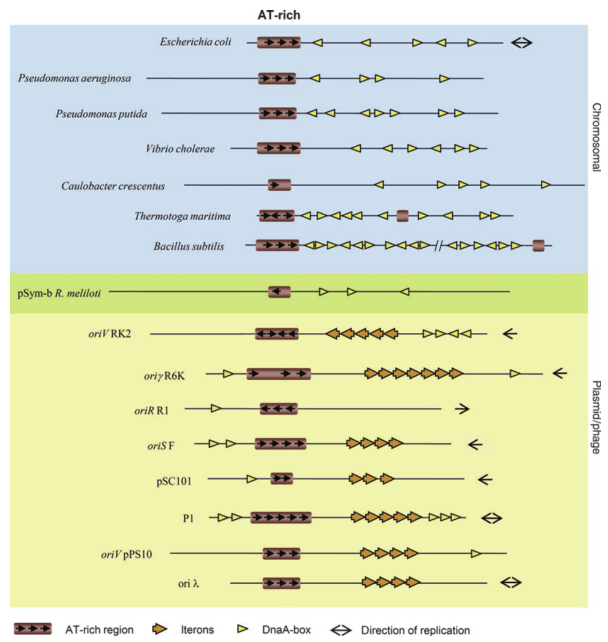
\includegraphics[height=0.5\textheight]{./img/ori_diversite.png}
			\caption[Diversité structurale des origines de réplication chez les bactéries]{Diversité des origines de réplication des réplicons bactériens chromosomiques et plasmidiques. Adapté de \citep{rajewska2012rich}. }\label{ori_div}
		\end{center}
\end{figure} 

\begin{description}
\item[$\blacktriangleright$] La structure des \textit{ori} plasmidiques présente certaines spécificités:
	\begin{description}
	\item[$\bullet$] La structure des \textit{ori} des plasmides à réplication thêta présente une organisation similaire à celles des chromosomes: DUE + motifs structuraux (Figure \ref{ori_div}). De nombreuses origines plasmidiques comportent des boîtes DnaA \citep{rajewska2012rich}, ce qui indique l'existence d'une interaction forte entre des régulateurs de l'hôte et la réplication plasmidique \citep{Kruger2004}. Les \textit{ori} plasmidiques peuvent également posséder des motifs spécifiques organisés en tandem, les itérons, qui permettent la fixation des protéines Rep et ainsi l'ouverture d'\textit{ori}. 
	\item[$\bullet$] L'origine de réplication chez les plasmides de type RC est un peu particulière car elle comporte deux origines: \textit{dso} (double strand origin) et \textit{sso} (single strand origin). La première est le lieu d'ouverture de l'ADN double brin. Elle comprend deux sites spécifiques: \textit{nick}, lieu de la coupure de l'ADN, et \textit{bind}, lieu de fixation de la protéine Rep. C'est à son niveau que s'amorce la réplication d'un des deux brins. L'autre origine, \textit{sso}, est l'endroit où est initiée la réplication de l'autre brin \citep{khan2005plasmid}. 
	\item[$\bullet$] Les plasmides SD sont majoritairement les plasmides de la famille IncQ \citep{Loftie-Eaton2012}. Leur origine est structurée en trois itérons correspondant au site de fixation de RepC, deux régions riches en G+C et A+T, respectivement, et deux sites d'initiation simple brin: \textit{ssiA} et \textit{ssiB} (\textbf{s}ingle \textbf{s}trand \textbf{i}nitiation A et B).
	\end{description}
\end{description}
  
\subsubsection{Déroulement de l'initiation}
\begin{description} 

\item[$\bullet$] Dans le modèle classique de l'initiation de la réplication du chromosome, l'attachement de plusieurs DnaA sur les boîtes DnaA d'\textit{ori} provoque une distorsion de l'ADN et conduit à son ouverture. Ce phénomène est suivi de la formation du complexe d'initiation (\textit{orisome}), et de l'action de l'hélicase sur l'ADN ouvert \citep{Robinson2005}. Chez \textit{E.coli}, Fis initialement présent est déplacé, ce qui permet la fixation de IHF et la formation d'un complexe protéique: le \textit{réplisome}  \citep{Mott2007,zakrzewska2007regulation}. L'ouverture est stabilisée par la fixation de protéines SSB qui protègent l'ADN simple brin.
\item[$\bullet$] L'initiation de la réplication thêta des plasmides est assez similaire à celle du chromosome bactérien: la fixation des protéines Rep sur les itérons provoque un changement de conformation de l'origine ce qui entraîne son ouverture. Des facteurs additionnels (DnaA, IHF, Fis, IciA, SeQ)  peuvent intéragir avec Rep ou se fixer à l'\textit{ori} afin de stabiliser/déstabiliser le complexe \citep{Kruger2004}.  
\item[$\bullet$] Chez les plasmides RC l'ouverture de l'ADN s'effectue au niveau du site \textit{nick} du site \textit{sdo} par fixation de la protéine Rep. Rep recrute ensuite une hélicase spécifique de l'hôte, PcrA (\textbf{P}lasmid \textbf{c}opy number \textbf{r}eduction protein \textbf{A}), qui étend l'ouverture. Un manteau de protéines SSB stabilise un des brins de l'ADN pendant que le complémentaire de l'autre brin est synthétisé par l'ADN polymérase III de l'hôte. La réplication du deuxième brin commence au site \textit{sso} et fait également intervenir la machinerie réplicative de l'hôte: ADN polymérase I et III, ADN gyrase et ADN ligase \citep{khan2005plasmid}.
\item[$\bullet$] L'initiation de la réplication des plasmides SD commence par la fixation de RepC au niveau des itérons, ce qui induit une rupture de la structure de l'origine et conduit à son ouverture. RepA pénètre alors dans l'ouverture et catalyse le déroulement de l'ADN. Lorsqu'ils sont à découvert, les sites \textit{ssiA} et \textit{ssiB} sont reconnus par RepB qui permet la fixation de l'ADN polymérase III et le début de la réplication grâce aux amorces synthétisées par RepB \citep{Loftie-Eaton2012}.
\end{description}
Contrairement à certains plasmides à réplication thêta, les plasmides SD et RC nécessitent une intervention réduite des protéines de l'hôte. Il est alors intéressant de constater qu'au final, \textbf{\color{orange} l'initiation de la réplication du chromosome n'est qu'un cas particulier de celle des plasmides thêta}.


\subsubsection{Régulation de l'initiation}
	Les modèles classiques de régulation de l'initation de la réplication impliquent majoritairement deux types de processus selon leur cible:
\begin{itemize}
	\item La séquestration, la déstabilisation ou l'occupation d'\textit{ori} et de ses motifs structuraux.
	\item L'inactivation, la séquestration ou la régulation des protéines initiatrices, Rep et DnaA.
\end{itemize}

\begin{description}
\item[$\blacktriangleright$] L'initiation de la réplication du chromosome est très précisément régulée pour garantir qu'une unique réplication du chromosome aura lieu au cours d'un cycle cellulaire.
	\begin{description} 
		\item[$\bullet$] Les mécanismes de séquestration de l'origine de réplication du chromosome chez \textit{E. coli} font intervenir les motifs GATC (GANTC chez \textit{B. subtilis}) et les protéines Dam qui méthylent ces sites au niveau de leur adénine. Avant initiation de la réplication, les sites GATC de l'origine sont doublement méthylés sur les brins direct et indirect (GATC étant un palindrome, si on considère son complémentaire). Juste après l'initiation, ces sites se retrouvent hémiméthylés car le brin néo-synthétisé n'a pas encore été soumis à l'action de Dam. Cette hémiméthylation conduit à la fixation de SeqA, ce qui empêche la fixation de DnaA au niveau de la nouvelle origine \citep{Mott2007,Kruger2004}. La séquestration de l'\textit{ori} par SeqA et Dam semble être une caractéristique des Entérobactéries, mais divers mécanismes de séquestration existent pour d'autres bactéries \citep{zakrzewska2007regulation}. Chez \textit{B. subtilis}, la séquestration d'\textit{ori} se fait par deux protéines non homologues de SeqA, Spo0A et SirA \citep{Katayama2010}.
		\item[$\bullet$]  La régulation de DnaA chez \textit{E.coli} implique aussi la titration des protéines au niveau d'une séquence caractéristique, le locus \textit{datA}, avec pour effet de réduire le nombre de DnaA actives disponibles.
		\item[$\bullet$]  Le mécanisme RIDA (Regulatory inactivation of DnaA) \citep{Mott2007} permet le passage de la forme active de DnaA, DnaA-ATP, à la forme inactive, DnaA-ADP, par l'intervention des protéines HdA et d'une des sous-unités de l'ADN polymérase III chez \textit{E. coli} \citep{Katayama2010}. Ces mécanismes semblent aussi exister chez d'autres bactéries \citep{zakrzewska2007regulation}.
		\item[$\bullet$]  DnaA a aussi un rôle de facteur de transcription en se fixant sur les promoteurs de certains gènes. Elle exerce aussi une auto-inhibition de sa synthèse en se fixant au promoteur de son gène \citep{zakrzewska2007regulation}.
	\end{description}
	
\item[$\blacktriangleright$] Différents mécanismes de régulation de l'initation sont spécifiques des plasmides.
	\begin{description} 
		\item[$\bullet$]  Des mécanismes de séquestration d'\textit{ori} existent également chez les plasmides. Un exemple en est le \textit{handcuffing} de l'origine de réplication des plasmides à réplication thêta et à itérons. Les \textit{ori} des deux plamides néo-formés se lient \textit{via} les protéines Rep fixées, empêchant leur accès \citep{Kruger2004}.
		\item[$\bullet$]  Le contrôle de la disponibilité en protéines Rep chez les plasmides  dépend notamment de l'auto-régulation de la transcription des gènes \textit{rep}. Il peut aussi passer par la structure-même de l'\textit{ori} qui peut titrer Rep grâce à ses itérons ou des sites annexes \citep{Kruger2004}. Certaines protéines initiatrices Rep, activatrices dans leur forme monomérique, peuvent former des dimères et alors devenir inhibitrices de la réplication \citep{Kruger2004,Cervantes-Rivera2011}. L'équilibre thermodynamique étant plutôt en faveur des dimères, l'introduction d'un plasmide dans un hôte qui abrite déjà un plasmide utilisant la même protéine Rep aura tendance à ne pas pouvoir se répliquer, l'initiation étant directement bloquée par les dimères de protéines Rep des plasmides présents. Ainsi les protéines Rep interviennent aussi dans les mécanismes dit d'“incompatibilité plasmidique”.
		\item[$\bullet$]  Des inhibitions par intervention d'ARN anti-sens agissant au niveau de la régulation de l'initiation plasmidique ont été caractérisées \citep{brantl2004plasmid}. L'inhibition intervient majoritairement dans le blocage de la traduction de l'ARNm des protéines activatrices Rep (par exemple, chez le plasmide R1 d'\textit{E. coli}) ou en se fixant au niveau de leurs cibles. Dans le cas des plasmides de type “RepABC”, le gène de l'activateur de l'initiation RepC étant inclus dans un opéron regroupant \textit{repA} et \textit{repB} (homologues de \textit{parA} et \textit{parB}, respectivement), la synthèse de RepC peut être pseudo-auto-inhibée par RepA et/ou RepB \citep{Pinto2012}, ou inhibée par un ARN antisens dont le gène est présent à l'intérieur même de l'opéron \citep{Cervantes-Rivera2011}. Enfin, de nombreuses protéines de l'hôte (DnaA, IHF, Fis) peuvent intervenir dans la régulation des gènes \textit{rep} ou participer à l'inactivation des protéines Rep, ainsi que dans l'activation/inactivation des \textit{ori} plasmidiques \citep{Kruger2004}. 
	\end{description}
\end{description}


\subsection{Élongation}
	Après la formation du replisome, l'ADN est répliqué bidirectionnellement chez les chromosomes et la majorité des plasmides à réplication thêta, et unidirectionnellement chez les autres, les plasmides à réplication RC et SD et certains plasmides à réplication thêta. Les protéines clé formant les complexes de réplication organisés aux deux fourches de réplication, sont les suivantes: 
\begin{itemize}
\item une hélicase faisant passer l'ADN du stade double-brin au stade mono-brin,
\item des molécules stabilisatrices de l'ADN mono-brin (SSB),
\item des primases synthétisant des amorces ARN nécessaires à la formation des fragments d'Okazaki,
\item des polymérases synthétisant l'ADN et/ou remplaçant l'ARN par de l'ADN,
\item des systèmes de correction d'erreur,
\item des ligases liant les différents fragments synthétisés.
\end{itemize}
	Deux types de protéines additionnelles sont nécessaires au bon fonctionnement des polymérases: des protéines d'attache à l'ADN (pinces), qui forment généralement un anneau glissant autour de l'ADN, et des protéines permettant l'établissement des protéines pinces sur l'ADN. Les principales protéines impliquées dans l'élongation sont présentées Table \ref{tabelongprot}. Une bonne revue des différents mécanismes moléculaires impliqués dans l'élongation peut être trouvée dans \citep{Johnson2005a}. 
  
\begin{longtable}{@{\hspace{-2cm}\hspace{1cm}} >{\bfseries}p{0.2\textwidth} | >{\small}p{0.9\textwidth}}
	\caption{Principales protéines impliquées dans l'élongation}\label{tabelongprot}\\
	\endfirsthead
	holoenzyme, \mbox{ADN} \mbox{polymérase III} & L'ADN polymerase III est un complexe comprenant différentes protéines (10 chez \textit{E. coli}), incluant les polymérases cœur, la pince glissante et cinq sous-unités responsables du chargement de la pince sur l'ADN. Ces protéines ont été plus particulièrement détaillées chez les bactéries Gram négatif (\textit{E. coli} surtout) mais semblent être retrouvées chez l'ensemble des bactéries ainsi que chez les Archées \citep{o2013principles}.\\
	Pol III core & Ces protéines interviennent dans les fonctions polymérase (\textbf{DnaE}) et 3'-5' exonucléase (\textbf{DnaQ}).\\
	\\[-0.2cm]
	DnaN & Pince circulaire de l'ADN polymérase III.\\
	\\[-0.2cm]
	Complexe d'attache de la pince & Chez \textit{E. coli}, cinq sous-unités sont responsables du chargement de la pince: \textbf{DnaX} (partie mobile), \textbf{HolA} (ouverture de la pince), \textbf{HolB} (partie fixe), \textbf{HolC} (protéine de transfert) et \textbf{HolD} (stabilisateur).\\
	\\[-0.2cm]
	PolA & ou ADN polymérase I. Enlève les amorces ARN par sa fonction exonucléase.\\
	\\[-0.2cm]
	DNA ligase I & Lie les fragments d'Okazaki en un seul fragment continu.\\
	\\[-0.2cm]
	GyrA et GyrB & protéines de type topoisomérase. Elles ont pour rôle de relaxer les superenroulements créés dans l'ADN lors de la réplication et par l'action des hélicases. Les topoisomérases peuvent être classées en deux catégories selon qu'elles agissent sur l'ADN double ou simple brin. GyrA et GyrB sont les deux sous-unités de la topoisomérase II d'\textit{E. coli} et agissent sur l'ADN double brin.\\
\end{longtable}

Une particularité de la réplication des plasmides SD, est qu'en plus d'être unidirectionnelle, il n'y a pas de production de fragment d'Okazaki pendant celle-ci. Les réplications SD et RC ont de plus la particularité de générer, durant la réplication, un intermédiaire d'ADN simple brin. Celui-ci étant hautement instable, ces types de réplication sont limités aux petits réplicons. 


\subsection{Terminaison de la réplication et résolution de dimère de réplicon}\label{ter}
 
\subsubsection{Mécanismes de terminaison de la réplication}
	Trois modèles décrivent actuellement la terminaison de la réplication des réplicons bactériens \citep{kono2012validation}:
\begin{itemize}
	\item le modèle \textbf{\textit{fork collision}} (collision de fourches) où la réplication bidirectionnelle s'interrompt lorsque les réplisomes des deux fourches de réplication se rencontrent. 
	\item le modèle \textbf{\textit{fork trap}} (piégeage de fourche) impliquant des associations ADN/protéine de type \textit{ter}/Tus qui entravent la progression de la polymérase à des sites spécifiques. Une protéine (Tus chez \textit{E. coli}, RTP (\textbf{R}eplication \textbf{T}erminaison \textbf{P}rotein) chez \textit{B. subtilis} \citep{kono2012validation}) se fixe sur l'ADN de façon site-spécifique et intéragit avec les protéines du réplisome afin de les déstabiliser \citep{kono2012validation,Johnson2005a}. 
	\item le modèle \textit{\textbf{dif-stop}}, contrairement aux deux précédents, implique une terminaison de la réplication à un site unique et précis.
 \end{itemize}
	Le modèle type \textit{ter}/Tus a été caractérisé pour le chromosome d'\textit{E. coli}. La région de la terminaison est bi-polarisée par une distribution de motifs \textit{ter}, orientés selon le sens de la réplication, de part et d'autre du site \textit{dif}. La protéine Tus n'est pas conservée dans le domaine bactérien et son homologue fonctionnel chez \textit{B. subtilis}, RTP, diffère tant au niveau structurel que par sa séquence, ce qui suggère une évolution relativement récente du modèle \textit{fork trap} \citep{kono2012validation}. 
	Les chromosomes ne possédant pas d'homologues fonctionnels des protéines \textit{Tus} (\textit{e.g.}, Firmicutes), ainsi que les plasmides à réplication thêta, semblent posséder un modèle d'arrêt de la réplication de type \textit{fork collision} \citep{kono2012validation}. Les plasmides se répliquant de façon unidirectionnelle n'utilisent pas d'appareil de terminaison ni ne suivent le modèle par collision de fourches.\\
Dans la terminaison de la réplication des plasmides de type RC, les protéines Rep semblent impliquées en promouvant une coupure de l'ADN au niveau du site d'ouverture \textit{dso}, ce qui libère un réplicon néo-formé ainsi qu'un intermédiaire simple brin \citep{,DelSolar1998,khan2005plasmid}. Chez les plasmides SD la réplication finit de même au site d'ouverture, la réplication étant monodirectionnelle \citep{Loftie-Eaton2012}.\\
	Les principales protéines jouant un rôle dans la terminaison de la réplication sont présentées Table \ref{tabrepelong}.

\begin{longtable}{@{\hspace{-2cm}\hspace{1cm}} >{\bfseries}p{0.2\textwidth} | >{\small}p{0.9\textwidth}}
	\caption{Principales protéines impliquées dans la terminaison de la réplication} \label{tabrepelong} \\
	\endfirsthead
	ParC & Sous-unité A de la topoisomérase IV. Trouvée chez \textit{E. coli} et \textit{B. subtilis} \citep{barnes2003dna}.\\
	\\[-0.2cm]
	ParE & Sous-unité B de la topoisomérase IV. Trouvée chez \textit{E. coli} et \textit{B. subtilis} \citep{barnes2003dna}.\\
	\\[-0.2cm]
	FtsK/SpoIIIE/ Tra & FtsK (\textbf{F}ilamenting \textbf{t}emperate \textbf{s}ensitive protein \textbf{K}; SpoIIIE chez \textit{B. subtilis)} Translocase essentielle impliquée dans le cycle cellulaire et coordonnant les dernières étapes de la cytokinèse chez \textit{E. coli} \citep{graham2010ftsk} en intéragissant avec \textbf{ParC} et \textbf{XerD} \citep{barre2000ftsk}. Sa structure héxamérique entoure l'ADN et interagit avec \textbf{FtsZ, FtsQ, FtsL} et \textbf{FtsI}, autres protéines impliquées dans le cycle cellulaire. Cette famille de translocases est très conservée chez les bactéries (sauf les Cyanobactéries) \citep{bigot2007ftsk}. \textbf{Tra}, translocase trouvée chez certains éléments mobiles et impliquée dans la conjugaison, appartient à la même famille protéique \citep{bigot2007ftsk}.\\
	\\[-0.2cm]
	Tus & Cette protéine se fixe sur les motifs \textit{ter} et déstabilise les protéines du réplisome lorsque celui-ci est à proximité d'un complexe Tus-\textit{ter}. Elle est présente chez \textit{E. coli} et quelques Entérobactéries proches. Ni Tus, ni \textit{ter} ne sont conservés parmi les chromosomes bactériens.\\
	\\[-0.2cm]
	\mbox{Recombinases} \mbox{site-spécifiques} & \textit{cf.} ci-dessous.
\end{longtable}

Une des caractéristiques essentielles des sites de terminaison de la réplication chez les bactéries est qu'ils sont directement liés aux mécanismes moléculaires impliqués dans la résolution de dimère de réplicon.

 
\subsubsection{Résolution de dimère au niveau du site de terminaison}\label{dimere}
	Au cours de la réplication des réplicons chromosomiques ou plasmidiques, des dimères peuvent apparaître, où les deux intermédiaires de réplication ne forment qu'une seule molécule \textit{via} des processus de recombinaison homologue \citep{Johnson2005a}. La formation d'un dimère altère non seulement la ségrégation active des chromosomes et plasmides, mais perturbe également la réplication. Un multimère ayant plusieurs origines de réplication aura tendance à être sur-répliqué, ce qui peut conduire à l'épuisement de l'espace et des ressources disponibles de l'hôte  \citep{hallet2004dna}. Dans le cas des plasmides, il y a multimérisation du plasmide jusqu'à ce que le nombre de molécules disponibles lors de la division cellulaire ne soit pas suffisante pour assurer sa stabilité \citep{summers1984multimerization}. Ces phénomènes ne sont pas marginaux; chez \textit{E. coli}, 10 à 15\% des réplications entraînent la formation de dimère \citep{perals2000functional}.\\
	La résolution de dimère de chromosomes ou de plasmides requiert l'intervention d'une machinerie moléculaire dédiée impliquant des recombinases spécifiques, dont les principales représentantes sont le couple de protéines XerC/XerD. Ces recombinases agissent au niveau d'un site spécifique (site \textit{dif} des chromosomes) situé au niveau de la région de la terminaison de la réplication. Pour les plasmides, il existe différentes familles de recombinases qui présentent des mécanismes distincts (détaillées plus loin). Les sites de recombinaison sont eux-aussi différents de ceux des chromosomes \citep{hallet2004dna}. Contrairement au processus de recombinaison homologue, les systèmes de résolution de dimère impliquent une seule étape de recombinaison site-spécifique, indépendamment du cycle cellulaire pour les plasmides \citep{hallet2004dna} ou faisant intervenir FtsK pour les chromosomes. \\
	Ces systèmes dédiés sont bien conservés parmi les chromosomes bactériens ainsi que pour de nombreux plasmides \citep{thomas2004}.

 
 \subsubsection{Décaténation des régions terminales par les topoisomérases}
	Un autre obstacle à la séparation réussie des deux réplicons néo-formés est l'enchevêtrement des deux régions terminales \citep{thanbichler2010}. Les mécanismes impliqués dans la décaténation des deux réplicons font aussi intervenir FtsK qui interagit directement avec ParC et ParE, les deux sous-unités de la topoisomérase IV, impliquée dans la résolution des super-enroulements. En stimulant l'interaction de ParC et ParE entre la fin de la réplication et la séparation des cellules, FtsK permet l'activation de la topoisomérase IV \citep{thanbichler2010}. 



 \section{Partition active des réplicons}\label{segreg}
	Après qu'un réplicon a été correctement répliqué, chacun des deux exemplaires obtenus doit être ségrégé dans une des deux cellules fille en formation. Cette ségrégation peut être passive comme, par exemple, dans le cas des petits plasmides à taux de copie élevé \citep{Ebersbach2005} où les réplicons sont transmis de façon aléatoire à l'une des cellules fille. Dans le cas des réplicons à faible taux de copie, de grande taille et/ou d'une relative importance pour la vie de la bactérie, des mécanismes moléculaires sont nécessaires pour assurer une ségrégation réussie et la stabilité du matériel génomique au cours des générations. Il existe de grandes similarités entre les différents systèmes moléculaires de \textbf{partition} permettant une ségrégation active, présents chez les réplicons bactériens \citep{funnell2004partition}. Les acteurs majoritaires de ces systèmes sont les protéines de type \textbf{ParA} (ParA-\textit{like}), \textbf{ParB} (ParB-\textit{like}), ainsi que la séquence de type centromérique \textit{\textbf{parS}}(Table \ref{protseg}).
	 
 \begin{longtable}{@{\hspace{-2cm}\hspace{1cm}} >{\bfseries}p{0.2\textwidth} | >{\small}p{0.9\textwidth}}
\caption{Principales protéines impliquées dans la ségrégation des réplicons}\label{protseg}\\
\endfirsthead
  MRP & protéine fixant l'ATP, impliquée dans la ségrégation des chromosomes. \\
	\\[-0.2cm]
 ParA/SopA/ ParM & Par commodité ces protéines seront désignées sous l'appellation: ParA-\textit{like} et les gènes les codant, \textit{parA-like}. Les protéines ParA-\textit{like} peuvent agir en tant que répresseurs des gènes \textit{parA} et/ou \textit{parB}. Ce sont des NTPases qui utilisent l'énergie libérée par hydrolyse de l'ATP et mettent en mouvement les réplicons par des phénomènes de polymérisation. Selon les ParA-\textit{like}, différentes configurations peuvent être prises par les polymères, bien que la conformation générale semble être similaire à celle des microtubules. Trois catégories de ParA-\textit{like} peuvent être distinguées: les \textit{Walker-A P-loop} ATPases (ParA, SopA; type I), les \textit{actin-like} ATPases (ParM;  type II) et les \textit{tubulin-like} ATPases (TubZ; type III) \citep{Mierzejewska2012,funnell2004partition}. Deux sous-types de ParA type I sont identifiés selon leur structure: Ia (ParA des plasmides F et P1) et Ib (protéines plus courtes) \citep{Passot2012}. Les ParA-\textit{like} de type II (ParM) ont la capacité de former des polymères avec une architecture très similaire à celle de l'actine chez les eucaryotes. Les ParA-\textit{like} de type III ont été caractérisées plus récemment chez des plasmides de \textit{Bacillus cereus} \citep{zheng2013evolution}. Ce sont des GTPase, analogues des tubulines des eucaryotes. Les ParA des chromosomes sont usuellement de type I à quelques exceptions près (\textit{E. coli} notamment). \textbf{MreB}, protéine de structure liée au cycle cellulaire et vraisemblablement remplaçant ParA chez \textit{E. coli}, est proche de ParM structurellement \citep{Mierzejewska2012}.\\
	\\[-0.2cm]
  ParB/SpoB/ ParR & Par commodité ces protéines seront désignées sous l'appellation ParB-\textit{like} et les gènes les codant, \textit{parB-like}. Dans les premières phases de la ségrégation des réplicons, ces protéines s'attachent à leur séquence centromérique respective, \textit{parS} (parfois appelée \textit{parC}), et promeuvent la polymérisation des ParA-\textit{like} \citep{funnell2004partition}. Les ParB-\textit{like} possèdent aussi un rôle dans la régulation des systèmes de partition. Surexprimées, ces protéines, dans certains cas, inhibent les gènes autour de \textit{parS} \citep{funnell2004partition}. Les ParB-\textit{like} peuvent aussi jouer un rôle dans l'accrochage des réplicons à la membrane bactérienne \textit{via} d'autres protéines intermédiaires \citep{Toro2010,Mierzejewska2012}.
 \end{longtable}
 
	Ce système de partition aurait un fonctionnement similaire à celui de l'appareil mitotique eucaryote \citep{Mierzejewska2012}. L'étape initiale de la ségrégation de deux réplicons néo-formés débute par la fixation de la protéine ParB-\textit{like} sur la séquence centromérique \textit{parS}. Une fois assemblé, ce complexe peut interagir avec la protéine ParA-\textit{like}. Pour être actives, ces dernières nécessitent l'action de l'ATP. Différentes structures peuvent être formées et différentes modalités de ségrégations mises en œuvre selon la protéine ParA-\textit{like} impliquée \citep{Mierzejewska2012,funnell2004partition}. Le modèle général semble néanmoins impliquer une polymérisation des ParA-\textit{like}, ce qui a pour effet de “pousser” les réplicons aux pôles opposés d'une manière analogue à celle des microtubules  chez les Eucaryotes \citep{Mierzejewska2012}. La régulation des systèmes de partition se fait d'une part par la dépolymérisation naturelle des ParA-\textit{like}, et d'autre part par une régulation des gènes \textit{parA} et \textit{parB}, généralement regroupés dans un même opéron. Cette régulation fait intervenir les protéines ParA-\textit{like} et ParB-\textit{like} (autorégulation) ou des protéines annexes liées au cycle cellulaire \citep{Mierzejewska2012,funnell2004partition,Pinto2012}. Outre le système parABS, d'autres systèmes moléculaires peuvent ségréger les chromosomes bactériens. MukB et SMC (deux analogues) semblent par exemple être impliqués dans la ségrégation des chromosomes de \textit{E. coli} et de \textit{B. subtilis}, respectivement \citep{Toro2010}. Le système parABS est retrouvé chez la très grande majorité des réplicons bactériens, ce qui est en faveur d'une émergence ancienne et unique, potentiellement existant dès l'origine des premiers réplicons. Ces systèmes constituent de fait un point clé de caractérisation parmi les propriétés fondamentales des réplicons.



\section{Maintenance des réplicons et intégration dans le cycle cellulaire}\label{regul}
	Il existe un lien logique des contrôles de la réplication et des systèmes de ségrégation des réplicons avec le cycle cellulaire. Les divers mécanismes de maintenance développés par les réplicons permettent d'optimiser, en terme de coût énergétique et d'efficacité (\textit{i.e.}, minimiser le taux de processus défectueux), leur réplication/ségrégation au sein de l'hôte et leur maintien dans l'espace et le temps à travers le cycle cellulaire (Table \ref{maintenance}). De nombreux mécanismes moléculaires impliqués dans la structure des réplicons interviennent de fait dans la maintenance des réplicons. Classiquement, la fin de la réplication des chromosomes doit être suivie d'un détachement réussi des régions terminales des deux chromosomes, de processus de partition/ségrégation et des phénomènes de condensation selon un ordre précis \citep{thanbichler2010}. 
\\
\begin{longtable}{@{\hspace{-2cm}\hspace{1cm}} >{\bfseries}p{0.2\textwidth} | >{\small}p{0.9\textwidth}}
	 \caption[Principales protéines impliquées dans la maintenance et le cycle cellulaire]{Principales protéines impliquées dans la maintenance et le cycle cellulaire des réplicons bactériens}\label{maintenance}\\
	 \endfirsthead
	 AcrA & fait partie d'un complexe protéique servant au transfert de diverses molécules à travers la membrane. C'est un acteur clé dans le cycle cellulaire \citep{lau2005cell}. Son inhibition influence directement le fonctionnement moléculaire des protéines du divisiome \citep{li2011targeting}\\
	\\[-0.2cm]
	 AmiC & est une protéine périplasmique clôturant la formation du divisiome \citep{vicente2006septum}. \\
	\\[-0.2cm]
	 EzrA & est un régulateur négatif de l'assemblage de l'anneau de FtsZ chez \textit{B. subtilis} \citep{yamanaka1996identification}.\\
	\\[-0.2cm]
	 Fic & (Filamentation induced by cyclic AMP protein) est une protéine inductrice du cycle cellulaire chez \textit{E.coli} \citep{kawamukai1989nucleotide}. Elle est aussi présente chez \textit{B. subtilis}.\\
	\\[-0.2cm]
	 FtsZ & Protéine majeure impliquée dans la formation du septum et dans la division cellulaire. FtsZ s'assemble en anneau à l'équateur de la cellule, ce qui permet, par un mécanisme de constriction, de couper la membrane \citep{thanbichler2010}. FtsZ, très conservée parmi les bactéries (à une exception: \textit{Chlamydia}, \citep{li2011targeting}), est également présente chez certaines Archées \citep{vicente2006septum}.\\
	\\[-0.2cm]
	  FtsA & Protéine intervenant avec \textbf{ZipA} dans la formation de l'anneau FtsZ \citep{vicente2006septum}.\\
	\\[-0.2cm]
	  ZipA & s'accroche à FtsZ \textit{in vitro} et aide à la stabilisation de l'anneau de FtsZ \textit{in vivo} \citep{li2011targeting}. Tout comme FtsB, FtsL et FtsN, ZipA n'est pas retrouvée chez certaines bactéries \citep{li2011targeting}.\\
	\\[-0.2cm]
	  ZapA & Protéine participant avec FtsA et ZipA à la formation de l'anneau FtsZ \citep{vicente2006septum}.\\
	\\[-0.2cm]
	 FtsB, FtsE, FtsI, FtsN, FtsQ, FtsW, FtsX & protéines intervenant, après FtsA/ZipA, dans la stabilisation de l'anneau FtsZ \citep{vicente2006septum}.\\
	\\[-0.2cm]
	 GidA & (Glucose inhibited division protein A) protéine quasiment universelle dans les génomes bactériens, influe sur la réplication \citep{kinscherf2002global}. Ces protéines possèdent un domaine fonctionnel de type méthyltransferase.\\
	\\[-0.2cm]
	 GidB & (Glucose inhibited division protein B) est une protéine possédant, comme GidA, un domaine fonctionnel de type méthyltransferase. Tout comme GidA, GidB est probablement impliquée dans le cycle cellulaire \citep{ogasawara1992genes}. On la trouve aussi bien chez \textit{B. subtilis} que chez \textit{E. coli}.\\
	\\[-0.2cm]
	 TrmFO & est une protéine de la même famille que GidA qui semble également impliquée dans la division cellulaire \citep{cicmil2008crystallization}. Elle est généralement trouvée chez les bactéries à Gram positif.\\
	\\[-0.2cm]
	 SepF & est une protéine conservée chez les bactéries à Gram positif. Elle interagit avec FtsZ (chez \textit{B. subtilis}) et joue un rôle significatif dans le développement du septum \citep{hamoen2006sepf}.\\
	\\[-0.2cm]
	SlmA & Protéine fixant l'ADN et inhibitrice de l'assemblage de FtsZ \citep{thanbichler2010}. SlmA, présente chez \textit{E. coli}, est très peu conservée parmi les bactéries. \textbf{Noc} est son homologue fonctionnel chez \textit{B. subtilis}.\\
	\\[-0.2cm]
	  SulA & est une protéine du système SOS (réparation sur épreuve) caractérisée chez \textit{E. coli}. Elle est aussi impliquée dans l'arrêt de la division cellulaire en interagissant avec FtsZ \citep{yamanaka1996identification}. \\ 
	\\[-0.2cm]
	 MinC & est un inhibiteur de la formation de polymères de FtsZ par oscillations rapides entre les pôles de la cellule \citep{thanbichler2010}. \\
	\\[-0.2cm]
	 MinD & agit en concert avec MinC en s'attachant à celle-ci afin d'empêcher la polymérisation de FtsZ \citep{thanbichler2010}. \\
	\\[-0.2cm]
	 MinE & est organisée en anneau autour de la membrane et déplace progressivement la position des complexes MinCD \citep{thanbichler2010}. \\
	\\[-0.2cm]
	 MreB & est homologue de l'actine et est essentiel dans le maintien de la forme de bâtonnet d'\textit{E. coli}. Son inactivation entrave sérieusement la ségrégation des chromosomes \citep{Ebersbach2005}. MreB s'associe avec MreC et MreD. Elle est trouvée chez l'ensemble des bactéries.\\
	 \\[-0.2cm]
	 MreC et MreD & sont impliquées, en interaction avec MreB, dans la maintenance de la structure en forme de bâtonnet de la cellule et dans la ségrégation des chromosomes \textit{E. coli} \citep{wachi1989new}.\\
	\\[-0.2cm]
	MukB & joue un rôle central dans la condensation et la ségrégation de l'ADN, et le cycle cellulaire d'\textit{E. coli} \citep{thanbichler2010,yamanaka1996identification}. Cette protéine forme un complexe avec \textbf{MukE} et \textbf{MukF} et interagit avec \textbf{FtsZ} et la topoisomérase \textbf{ParC}.\\
	\\[-0.2cm]
	\mbox{MukE et MukF} & interagit avec MukB. MukF et MukE interagissent ensemble \citep{yamanaka1996identification}. \\
	\\[-0.2cm]
	 SMC & (Structural Maintenance of Chromosome) est un analogue de MukB. Elle joue un rôle central dans la condensation du chromosome et est liée à ScpA et ScpB.\\
	\\[-0.2cm]
	 ScpA et ScpB & sont deux protéines auxiliaires du complexe SMC. Elles ont été découvertes chez les bactéries à Gram positif et chez les Archées \citep{thanbichler2010}. ScpA s'accroche à SMC et est stabilisée par ScpB. Des mutations sur ScpA provoquent le même effet que des mutations sur SMC \citep{thanbichler2010}.\\
	\\[-0.2cm]
	  DivIVA & caractérisée chez \textit{B. subtilis}, est une protéine majeure du cycle cellulaire. Elle intervient en intéragissant ave minCD et régule la formation du septum \citep{edwards1997bacillus}. Elle est de plus associée à RacA \citep{OSullivan2011}.\\
	\\[-0.2cm]
	 RacA & est une protéine d'ancrage chez \textit{B. subtilis}. Elle accroche \textit{ori} aux pôles de la cellule afin de préparer la division cellulaire. Elle est associée à DivIVA \citep{OSullivan2011}.\\
	\\[-0.2cm]
	 RodA & est une protéine impliquée dans la division et l'élongation cellulaire. Elle est décrite chez \textit{B. subtilis} et \textit{E. coli} \citep{henriques1998control}.\\
	\\[-0.2cm]
	 Systèmes PSK & (Post Segregational Killing) Véritable système d'“addiction génique”, ces complexes géniques interviennent de façon indirecte dans la stabilité et la maintenance d'un élément génétique (plasmide, séquence d'insertion, phage, transposon, complexe allélique...). Ces systèmes sont classiquement organisés en un gène codant une toxine et un gène codant une antitoxine avec éventuellement un gène régulateur. Une modification dans le système (perte de l'antitoxine, perte du système, gradient de concentration...) peut entrainer une concentration trop importante de la toxine et la mort cellulaire. Il existe une variété de systèmes PSK: \textbf{higBA, mazEF, relBE, HOK/SOK, vapXD, parDE, epsilon-zeta, ccd, Phd/Doc}... \citep{kobayashi2004genetic}.\\
 \end{longtable}
 
	Les mécanismes moléculaires de la division cellulaire impliquent la protéine FtsZ comme “fer de lance”. Chez \textit{E. coli}, FtsZ forme une structure polymérique en forme d'anneau dirigeant le processus de la division cellulaire \citep{thanbichler2010}. L'intervention de protéines additionnelles est souvent requise pour contrôler la position et la formation du \textit{divisiome} (système protéique impliqué dans la division) telles que le système Min (impliquant les protéines \textbf{MinC, MinD} et \textbf{MinE}) et \textbf{SlmA} (chez \textit{E. coli}), Noc (chez \textit{B. subtilis}) ou le système \textbf{MipZ} chez \textit{Caulobacter crecentus} \citep{Thanbichler2010}. Une quinzaine de protéines supplémentaires (notamment \textbf{FtsA, FtsB, FtsE, FtsI, FtsN, FtsQ, FtsW, FtsX, ZipA, ZapA et AmiC}) particulièrement bien conservées parmi les réplicons bactériens, sont recrutées dans la formation du septum \citep{vicente2006septum}. Chez les plasmides, la réplication, bien qu'asynchrone par rapport au cycle cellulaire, doit être régulée pour i) éviter une multiplication anarchique des plasmides et aboutir à un épuisement des ressources de l'organisme (“runaway replication” \citep{DelSolar1998}), ii) dupliquer le matériel génétique au bon moment au bon endroit et, de ce fait, adapter le cycle plasmidique au cycle cellulaire, et iii) être transmis équitablement aux deux cellules fille de l'hôte originel \citep{Pinto2012}. Différents mécanismes moléculaires spécifiques sont utilisés par les plasmides pour se maintenir à moindre coût, en adéquation avec leur nature non-essentielle, potentiellement égoïste et asynchrone par rapport au cycle cellulaire. Les mécanismes dits d'addiction plasmidique, ou \textit{Post-Segregational Killing} (PSK), très largement représentés chez les plamides, sont caractérisés par l'installation dans le génome d'un complexe génique impliqué dans la production d'une toxine et de son antitoxine correspondante. Toute modification du complexe provoque la mort de l'hôte \citep{mochizuki2006genetic}. Ces systèmes sont avantageux pour les plasmides d'un point de vue évolutif car ils garantissent le maintien des plasmides dans l'hôte les hébergeant. Ils sont aussi présents sur les chromosomes et permettent, par exemple, la stabilisation d'un complexe allélique \citep{mochizuki2006genetic}. De façon générale, il est intéressant de constater que l'évolution des génomes a gardé de tels systèmes géniques au comportement égoïste: outre le maintien de populations plasmidiques \citep{mochizuki2006genetic}, ces systèmes peuvent contribuer à la maintenance chromosomique, comme par leur implication dans la survie de populations bactériennes en situation de carence ou faisant face à des éléments génétiques intrusifs (phages, transposons...) \citep{kobayashi2004genetic}. Ces systèmes sont également la preuve que \textbf{\color{orange}l'évolution des génomes bactériens a adapté des systèmes plasmidiques dans les processus de maintenance chromosomique (ou inversement).}

\section{Mécanismes moléculaires de recombinaison, d'intégration et de transfert génétique}\label{recom}
	Les recombinaisons génétiques sont des phénomènes d'échange de fragments entre deux molécules d'ADN. Elles nécessitent l'action de diverses protéines et enzymes dont les recombinases. On distingue la recombinaison homologue où des brins d'ADN sont échangés entre molécules homologues, des recombinaisons dite “site-spécifiques” pour lesquelles les enzymes agissent seulement au niveau de sites présentant des motifs structuraux particuliers. Les recombinaisons homologues sont majoritairement impliquées dans les phénomènes de réparation de l'ADN chromosomique pendant la réplication, où un des brins d'une première molécule d'ADN (double-brin) va recombiner avec un brin d'une deuxième molécule d'ADN endommagée et servir de matrice à différentes enzymes afin de corriger la lésion \citep{perry1997microbiology, Barre2005}. Elles interviennent aussi dans différents processus moléculaires chez les phages \citep{Lopes2010}.\\
	Contrairement aux processus de recombinaison homologue, les recombinaisons site- spécifiques sont réalisées par une machinerie moléculaire relativement simple où les recombinases vont prendre en charge les étapes de césure, d'échange et de fermeture de l'ADN \citep{hallet2004dna}. Elles ont lieu sur de courts segments d'ADN, les \textit{sites de recombinaison}. Les recombinaisons site-spécifiques interviennent notamment dans la résolution de dimère précédemment abordée, mais aussi, de façon très similaire, dans la réplication de certains transposons \citep{hallet2004dna}. Enfin, elles peuvent intervenir dans les processus d'intégration et d'excision des bactériophages et de différents éléments mobiles \citep{hallet2004dna}. 
 
 \subsection{Résolvases impliquées dans la résolution de dimère de réplicon}
	Plasmides et chromosomes, dans leur grande majorité, codent des systèmes protéiques de recombinaison homologue spécifiques à la résolution des dimères formés lors de la réplication. Les enzymes impliquées sont des \textbf{résolvases}. On en distingue deux familles: les tyrosine- et les sérine-recombinases (Table \ref{resolvases}). Cette distinction repose sur la nature de l'acide aminé servant en premier à l'attaque nucléophile de l'ADN par la recombinase.
\\
\begin{longtable}{@{\hspace{-4cm}\hspace{1cm}} >{\bfseries}p{0.3\textwidth} | >{\small}p{0.9\textwidth}}
\caption{Résolvases impliquées dans la résolution de dimère}\label{resolvases}\\
\endfirsthead
	Tyrosine-recombinases & Les tyrosine-recombinases présentent différents niveaux de complexité. Leur fonctionnement ne nécessite qu'un simple site de recombinaison ou peut impliquer des sites d'attache de protéines régulatrices. On trouve parmi elles les résolvases de type \textbf{Xer} qui sont un parfait exemple de protéine multi-usage, à mécanisme simple, et largement répandues parmi des plasmides et chromosomes bactériens. Le système Xer le mieux décrit fait intervenir deux protéines, \textbf{XerC} et \textbf{XerD}, qui effectuent la recombinaison homologue des réplicons au niveau du site \textit{dif}. Des homologues de ces protéines sont trouvés dans le génome de presque toutes les bactéries et archées ayant un chromosome circulaire \citep{hallet2004dna}\citep{cortez2010evidence}) et chez de nombreux plasmides, ce qui suggère une conservation stricte du système Xer/\textit{dif} pour les chromosomes bactériens \citep{Carnoy2009,Kono2011}. Il existe cependant des variations mono-protéiques au système XerCD. Dans le génome des firmicutes, une seule protéine homologue à XerC et XerD, \textbf{XerS}, fait office de résolvase \citep{Leroux2011}. Un autre système Xer chez une partie des epsilon-protéobactéries implique une unique recombinase, \textbf{XerH}, qui ne présente pas de lien phylogénique apparent avec XerS \citep{Carnoy2009}. Le système Xer/\textit{dif} n'est cependant pas présent de manière universelle. Certains génomes, principalement chez des endosymbiotes, ne semblent pas posséder de sites \textit{dif}, ni de protéines Xer \citep{Carnoy2009,Kono2011}. D'autres systèmes de recombinaisons, faisant notamment intervenir des sérines-recombinases, peuvent remplacer les systèmes Xer/\textit{dif} \citep{Carnoy2009}. Des résolvases différentes de la famille Xer peuvent exister et participer à la résolution des dimères chez certains plasmides, comme par exemple, les résolvases de la famille de ResD découvert chez un plasmide d'\textit{E. coli} \citep{hallet2004dna}. Enfin, les systèmes Xer/\textit{dif} chromosomiques fonctionnent différemment de ceux des plasmides. Ils requièrent l'intervention de protéines supplémentaires (FstK entre autres, \textit{c.f.} \ref{recom}) les liant au cycle cellulaire. \\
	\\[-0.2cm]
	Sérine-recombinases & Elles sont présentes sur les plasmides des bactéries à Gram positif ou négatif. Elles sont homologues des résolvases impliquées dans l'insertion de transposons et en sont clairement dérivées, pouvant d'ailleurs se substituer à celles de ces derniers \citep{hallet2004dna}. Le site de recombinaison est généralement proche des gènes codant les recombinases, ce qui facilite le transfert latéral d'un système fonctionnel. On en distingue plusieurs sous-familles: les recombinases de type Mu (proches des protéines du bactériophage Mu), de la famille Tn3 et les bêta-recombinases codées par certains plasmides de bactéries à Gram positif \citep{hallet2004dna}.
\end{longtable}
 
	Les chromosomes bactériens circulaires codent des tyrosine-recombinases, dont la grande majorité appartient au système XerC/XerD. Des homologues de ces protéines ont été identifiés chez de nombreux plasmides ainsi que chez des archées à génome circulaire \citep{hallet2004dna}. Les génomes linéaires ont des systèmes protéiques particuliers impliqués dans la résolution des télomères. Ces enzymes, les \textbf{ResT}, possèdent peu d'homologie de séquence avec les tyrosine-recombinases \citep{chaconas2005replication}. Les systèmes de résolution de dimère semblent avoir des fonctions annexes dans de nombreuses situations. Par exemple, ils peuvent être détournés par les phages pour s'insérer dans le génome de l'hôte ou permettre la conjugaison de leur génome \citep{Das2013,hallet2004dna} .
 
 
\subsection{Les autres recombinases}\label{parmge}
	Les familles des tyrosine- et sérine-recombinases incluent par ailleurs les “\textbf{transposases}”, impliquées dans l'insertion/excision des transposons, les “\textbf{relaxases}”, initiatrices de la réplication (Rep) et de la mobilisation (Mob) des plasmides RC, les “\textbf{intégrases}”qui catalysent les étapes d'intégration des rétrotransposons et rétrovirus, et certaines topoisomérases (Table \ref{MGE}). De manière générale, ces protéines catalysent des opérations d'excision/intégration de l'ADN et tiennent une place capitale dans les cycles des différents éléments génomiques mobiles (ou MGE pour \textit{Mobile genetic element}). 

\begin{longtable}{@{\hspace{-4cm}\hspace{1cm}} >{\bfseries}p{0.3\textwidth} | >{\small}p{0.9\textwidth}}
	\caption{Les recombinases distinctes des résolvases}\label{MGE}\\
	\endfirsthead
	DDE transposases & Ce sont des enzymes impliquées dans les cycles des transposons bactériens. L'action catalytique de ces enzymes impliquent trois acides aminés (Asp (D), Asp (D) et Glu (E), formant le motif DDE), qui coordonnent les transferts de groupement phosphoryle lors de la transposition \citep{higgins2005bacterial}. Ces transposases sont aussi présentes sur certains rétrovirus et rétrotranspons d'eucaryotes.\\
	\\[-0.2cm]
	Intégrases et transposases de type tyrosine-recombinase & Le système Cre/\textit{loxP} est un système de recombinaison trouvé chez le bactériophage P1 d'\textit{E. coli}. Il implique une unique recombinase \textbf{Cre} proche de l'intégrase \textbf{Int} du bactériophage lambda. Ce système est impliqué dans la circularisation des phages \citep{hallet2004dna}. Les tyrosine-recombinases comportent de plus des transposases codées par des transposons: Y2 ou RCT (pour Rolling Circle Transposition) \citep{higgins2005bacterial}, proches des protéines Rep des plasmides RC \citep{cornet2004non}, et les transposons Y codant une transposase plus classique.\\
	\\[-0.2cm]
	Intégrases et transposases de type sérine-recombinase & Plusieurs sérine-recombinases sont présentes en tant que transposases chez les transposons S \citep{higgins2005bacterial}. Tout comme pour les tyrosine-transposases, le site de transposition est moins contraint que le site de résolution \citep{cornet2004non}. Les intégrases des sérine-recombinases sont représentées par Hin et Gin, deux enzymes plasmidiques \citep{cornet2004non}. \\ 
	\\[-0.2cm]
 Relaxases & Cette famille hétéroclite d'enzymes regroupe en particulier les protéines qui se fixent sur le site de conjugaison des éléments conjugatifs et mobilisables, \textit{oriT}, et procèdent à son ouverture \citep{Guglielmini2013}. Ces protéines sont longues et comportent deux, ou plus, domaines fonctionnels (un domaine relaxase et un domaine hélicase). Différentes familles de relaxases sont identifiables et peuvent servir à classer les éléments conjugatifs \citep{Guglielmini2013}. Ces relaxases sont de plus structurellement homologues des protéines initiatrices de la réplication de type RC \citep{Smillie2010}.
\end{longtable}
 
 
\subsection{Les éléments transposables}\label{transposon}
	Les processus de recombinaison spécifique sont fortement impliqués dans les processus de ségrégation et de maintenance des réplicons bactériens. Ils sont à la base de la définition d'une classe d'éléments génétiques distincte des réplicons, les transposons (Table \ref{transposon}), bien que le type de recombinaison manifesté par les transposons diffère de la recombinaison site-spécifique impliquée dans la résolution de dimère de chromosome ou de plasmide. Différentes nomenclatures et types de transposons ont été définis selon leurs mécanismes d'insertion, les transposases impliquées, leurs sites d'insertion ou l'organisation de la séquence transposable \citep{Roberts2008, higgins2005bacterial}. 


\begin{longtable}{@{\hspace{-2.5cm}\hspace{1cm}}p{0.35\textwidth} | p{0.8\textwidth}}
	\caption{Principaux types de transposons}\label{transposon}\\
	\endfirsthead
	\textbf{Séquences d'insertion (IS)} & ou transposons unitaires. Ces séquences sont uniquement composées des structures (site de recombinaison) et gènes (transposases) impliqués dans la transposition.\\
	\\[-0.2cm]
	\textbf{Transposons composites} & sont composés d'IS et de gènes et structures additionnels codant, par exemple, des protéines de résistance aux antibiotiques.\\
	\\[-0.2cm]
	\textbf{Transposons conjugatifs} & ou ICE (\textit{Integrative Conjugative Element}) portent des gènes codant des fonctions d'excision et d'intégration (transposases/intégrases) et des fonctions de conjugaison \citep{Wozniak2010}.\\
	\\[-0.2cm]
	\textbf{Transposons mobilisables} & ou IME (pour \textit{Integrative Mobilisable Element}) peuvent être mobilisés entre cellules bactériennes, et codent en général leurs propres transposases \citep{Roberts2008}.\\
	\\[-0.2cm]
	\textbf{Îlots génomiques mobiles} & sont des séquences intégrées dans les génomes, codant leurs propres transposases, mais pas les gènes impliqués dans leur transfert inter-cellulaire. Ils contiennent des gènes modifiant le phénotype cellulaire (par exemple, îlots de pathogénicité) \citep{Boyd2009}.\\
	\\[-0.2cm]
	\textbf{Prophages transposables} & sont des génomes de bacteriophage intégrés dans des génomes bactériens et capable d'excision/insertion.\\
	\\[-0.2cm]
	\textbf{Prophages satellites} & sont des prophages déficients intégrés dans des génomes bactériens. Ils nécessitent l'intervention de la machinerie moléculaire d'autres prophages pour compléter leur cycle de réplication.\\
 \end{longtable}
 
 
	Ces éléments sont capables de s'insérer, en tant que fragments d'ADN discrets et non permutables, à différents sites dans les génomes \citep{higgins2005bacterial}. Par opposition aux réplicons, les éléments transposables ne sont pas capables de se maintenir et de se répliquer indépendamment de leur génome hôte. La transposition requiert l'action de transposases (\textit{c.f.} \ref{MGE}) qui catalysent les différentes réactions de coupure/jointure de l'ADN. Même si originellement les transposons ont été décrits comme codant des DDE transposases, une grande variété de transposons codent des transposases de type sérine- ou tyrosine-recombinase, dont certaines sont homologues des relaxases et des protéines Rep des réplicons RC \citep{Roberts2008}. Les transposons peuvent être soumis à des mécanismes de régulation contrôlant leur cycle d'excision/intégration, évitant de potentiels effets délétères à leur hôte. Ces mécanismes peuvent faire intervenir des ARN anti-sens, des protéines de méthylation (\textit{i.e.} Dam), des represseurs transcriptionnels ou des protéines de type NAP de l'hôte \citep{cornet2004non}. L'existence sur des ICE d'analogues de systèmes de partition a également été rapporté \citep{Wozniak2010}. 

 
 \subsection{Conjugaison des éléments génomiques} \label{conj}
	Un des derniers aspects de la description du matériel génomique bactérien concerne les mécanismes et structures impliqués dans la mobilisation des différents éléments génomiques. La \textbf{conjugaison} bactérienne est un des processus de dissémination de gènes entre cellules indépendamment de la reproduction \citep{lawley2004bacterial}. Elle implique le transfert d'ADN de cellule à cellule par contact avec établissement du canal de conjugaison, veritable “pont” moléculaire traversant les membranes cellulaires. Ce phénomène initialement décrit comme une spécificité plasmidique, a ensuite été caractérisé chez les ICE \citep{Wozniak2010}. Les systèmes de conjugaison sont constitués de trois sous-systèmes essentiels \citep{lawley2004bacterial,Smillie2010}:
\begin{itemize}
	\item Le transférosome (système de sécrétion de type IV: T4SS) qui est responsable de la déstabilisation de l'enveloppe cellulaire et de la synthèse du pilus.
	\item Le relaxosome, complexe protéique qui agit sur l'ADN au niveau de l'origine de transfert \textit{oriT}. Les enzymes du relaxosome sont responsables de l'ouverture du plasmide au site \textit{oriT} et du désenroulement de l'ADN grâce à des hélicases.
	\item Les protéines de couplage (T4CP) qui s'accrochent au transférosome et intéragissent avec la relaxase.
 \end{itemize}

	La conjugaison suit les étapes suivantes \citep{lawley2004bacterial}: i) Synthèse d'un pilus par la cellule donneuse et son intéraction avec la membrane de la cellule receveuse, suivie de la création d'un canal entre les deux membranes (\textit{mating pair formation}). ii) Intervention du relaxosome (et en particulier de la relaxase), qui coupe l'ADN de l'élément conjugatif au site \textit{nick}. Un des deux brins est alors “déroulé” et passe dans la cellule receveuse. iii) La réplication des deux molécules d'ADN simple brin dans les cellules par les machineries moléculaires des hôtes.\\
	La réplication des éléments conjugatifs est homologue à celle des plasmides de type RC. On distingue les éléments conjugatifs codant leur propre système T4SS, des éléments mobilisables possédant \textit{oriT}, relaxases et éventuellement un système T4CP \citep{Smillie2010}. Ces derniers peuvent être mobilisés et transférés à des cellules receveuses \textit{via} les systèmes T4SS et T4CP d'autres éléments conjugatifs.\\ 
	Il est remarquable que des modules fonctionnels d'ADN liés à la conjugaison et reliés d'un point de vue évolutif se retrouvent sur des plasmides de bactéries Gram-positif et Gram-négatif, ainsi que sur des transposons de type ICE et IME \citep{Francia2004}. De même, l'homogénéité relative des séquences \textit{oriT} identifiés sur certains plasmides et sur les ICE chez les bactéries Gram-positif et Gram-négatif suggère une origine ancienne \citep{Francia2004}. Ces homologies suggèrent que ces éléments génétiques ont évolués à partir d'un groupe de gènes et/ou de motifs d'ADN ancestraux qui ont divergé en s'adaptant à des situations particulières \citep{Francia2004}. 
 
 
 \section{Fluidité du matériel génétique}\label{parevoldesrepl}

“\textit{Rather than being a well-designed blueprint, a genome appears to be a temporary community of potentially mobile genes that essentially act selfishly}” \citep{mochizuki2006genetic}.\\\\

	Les différentes structures génomiques bactériennes et la relative diversité des mécanismes moléculaires impliqués dans les réplication, ségrégation et maintenance du génome laissent entrevoir la plasticité du génome bactérien. Les génomes sont soumis à des processus de modification et de transfert d'ADN internes, faisant intervenir un ou plusieurs éléments génétiques et réplicons, ou externes, impliquant plusieurs génomes bactériens (ou un génome et de l'ADN extra-cellulaire). Les échanges inter-génomiques sont généralement rassemblés sous la désignation de \textbf{T}ransfert \textbf{H}orizontal de \textbf{G}ènes (THG) et regroupent les processus de conjugaison (introduit dans la partie précédente), de transduction \citep{miller2004bacteriophage}, de transformation \citep{miller2004microbial}, ou encore les \textit{Gene Transfer Agents} plus récemment décrits. Les THG tiennent une part très importante dans l'évolution des génomes bactériens \citep{Wiedenbeck2011} et font intervenir des mécanismes moléculaires liés à la réplication, ségrégation et maintenance du génome. Ces mécanismes tiennent donc une place centrale dans la définition et l'évolution des génomes, notamment pour ce qui est de l'intégration et de la stabilisation dans l'organisme bactérien des différents éléments génomiques. Les mécanismes de recombinaison, en particulier, interviennent largement dans les échanges et inversions entre éléments génomiques. Les homologies structurelles et fonctionnelles partagées par les différentes classes de recombinases montrent des similitudes et indiquent de probables origines communes à ces molécules. Il semble de plus que l'on retrouve ces similitudes de manière plus générale (par exemple, avec les systèmes Par ou les systèmes conjugatifs). \textbf{Ainsi se dessine une continuité entre les différents réplicons et éléments génétiques retrouvés chez les bactéries ainsi que parmi les mécanismes moléculaires à l'œuvre dans leur maintenance.}	
 
\iffalse
\fi
 

\newpage
\chapter{Les réplicons extra-chromosomiques essentiels}\label{chap1b}
\lhead{\emph{Les réplicons extra-chromosomiques essentiels}}

\section{Découverte et premières caractérisations de génomes multipartites bactériens}
     
      Le modèle du génome bactérien que nous avons introduit dans le chapitre précédent repose essentiellement sur l'architecture du génome d'\textit{E. coli}, formé d'un unique chromosome circulaire et, éventuellement, de plasmides. Cette organisation proposée dans les années 1950 \citep{wollman1956conjugation} et mise en évidence par autoradiographie  du génome de \textit{E. coli} \citep{cairns1963chromosome}, fut plus tard retrouvée lors de l'étude de génomes additionnels, \textit{i.e.}, \textit{Bacillus subtilis}, et s'imposa alors comme la règle chez les bactéries. Ce modèle n'est cependant pas valide pour toutes les bactéries. Les génomes bactériens peuvent comporter plusieurs réplicons de type chromosomique (\textbf{génome multipartite}), et les réplicons bactériens, chromosomes et plasmides, pouvent être circulaires ou linéaires \citep{baril1989linear,kolsto1997dynamic,casjens1998diverse}.\\
       Les premières preuves de génomes multipartites bactériens apparurent avec la caractérisation par électrophorèse en champ pulsé du génome de \textit{Rhodobacter sphaeroides} à la fin des années 1980, qui permit de réaliser la seconde carte physique de génome  bactérien, après celle d'\textit{E. coli} \citep{suwanto1989physical,suwanto1989physicala}. Ces résultats mirent en évidence que deux des réplicons de \textit{R. sphaeroides} portent des gènes codant des ARNr et sont strictement essentiels pour la bactérie. Ces réplicons furent alors désignés par les termes de chromosome primaire (pour le plus grand) et chromosome secondaire \citep{suwanto1989physical}. Ces approches méthodologiques ont par la suite mis en évidence la présence de multiples réplicons essentiels chez \textit{Leptospira interrogans} \citep{zuerner1993comparison}, \textit{Brucella} \citep{michaux1993presence}, \textit{Pseudoalteromonas haloplanktis} \citep{lanoil1996marine}, \textit{Burkholderia} \citep{rodley1995physical} et \textit{Vibrio cholerae} \citep{trucksis1998vibrio}.\\           
        Depuis, les progrès des techniques de séquençage ont permis d'obtenir les séquences complètes de milliers de génomes bactériens révélant ainsi une grande diversité quant au nombre de chromosomes et de plasmides par complément génomique, à leurs tailles, et à leurs topologies, ainsi qu'une hétérogénéité de répartition de ces caractéristiques parmi les différentes lignées bactériennes \citep{casjens1998diverse,Mackenzie2004}. L'étude du catalogue, toujours plus important, des génomes dont la séquence complète est disponible, ainsi que la compréhension du développement bactérien \textit{in vivo} et \textit{in vitro} montrent qu'il existe non seulement des réplicons accessoires de taille et de complexité génomiques proches de celles des chromosomes mais que la limite entre réplicon essentiel et réplicon accessoire peut être difficile à définir \citep{Mackenzie2004}.\\ 
	Pour certains auteurs, le statut des réplicons dépend avant tout des caractéristiques structurales de ceux-ci  \citep{harrison2011bacterial}. Des études des structures d'\textit{ori} de chromosomes secondaires ont montré de grandes similarités avec les \textit{ori} de mégaplasmides, rapprochant ces deux types de réplicons d'un point de vue évolutif et fonctionnel. Différents modules génétiques ou gènes spécifiques, typiques des plasmides (tels que les gènes impliqués dans la conjugaison), sont retrouvés sur les chromosomes secondaires. Une autre ambiguïté provient de la distinction classique, conforme au dogme du chromosome bactérien unique, entre les différents réplicons essentiels d'un génome bactérien multipartite: on parle alors d'un chromosome \textit{primaire} et de chromosome secondaire ou mégaplasmide \citep{MacLellan2004} pour les \textbf{R}éplicons \textbf{E}xtra-\textbf{C}hromosomiques \textbf{E}ssentiels (\textbf{RECE}) sur la base de caractéristiques telles que la taille des réplicons, le nombre de gènes ou la présence de gènes essentiels.


\section{Diversité actuelle des génomes multipartites bactériens}\label{diversite}
	\definecolor{deepblue}{rgb}{1,0.5,0}
	Les occurrences de génomes multipartites dans les différentes lignées bactériennes sont hautement variables. Les génomes multipartites sont disséminés de façon irrégulière à travers la phylogénie des bactéries (Figure \ref{figphylgeco}). Les Protéobactéries semblent être leur phylum de prédilection car on les observe beaucoup plus fréquemment chez les Alpha-, Bêta- et Gamma-protéobactéries. Chez les Alpha-protéobactéries, jusqu'à 10 genres bactériens différents comportent au moins une espèce à génome multipartite. Par contre, le phylum des Firmicutes n'en comporte que peu  (deux génomes multipartites répertoriés) au regard du nombre d'espèces dont le génome a été complètement séquencé (745 espèces dans 90 genres taxonomiques). Néanmoins, la présence de réplicons secondaires essentiels a été relevée dans la plupart des lignées bactériennes majeures telles que les Spirochètes (\textit{Leptospira}), les Bacteroidetes (\textit{Prevotella}), les Firmicutes (\textit{Butyrivibrio} et \textit{Clostridium}), ou encore les Cyanobactéries (\textit{Anabaena} et \textit{Cyanothece}) (Table \ref{tabess}; Annexe \ref{AppendiceA}). Chez les Protéobactéries, 19 genres sur 231 contiennent au moins une espèce possédant un génome multipartite, pour seulement deux des 90 genres de firmicutes, soit quatre fois moins. Cela traduit peut-être simplement un échantillonnage déséquilibré vers les organismes pathogènes ou symbiotiques pour des raisons médicales et/ou économiques. L'écologie et le génome d'espèces telles que \textit{Candidatus} Chloroacidobacterium thermophilum \citep{GarciaCostas2012} ou \textit{Ilyobacter polytropus} \citep{Sikorski2010} en sont des contre-exemples, témoignant de l'effort récent pour étendre l'acquisition de données de séquences aux bactéries de l'environnement et à l'ensemble des bactéries, et plus généralement du vivant.  \\

\begin{figure}[H]
	\begin{center}
	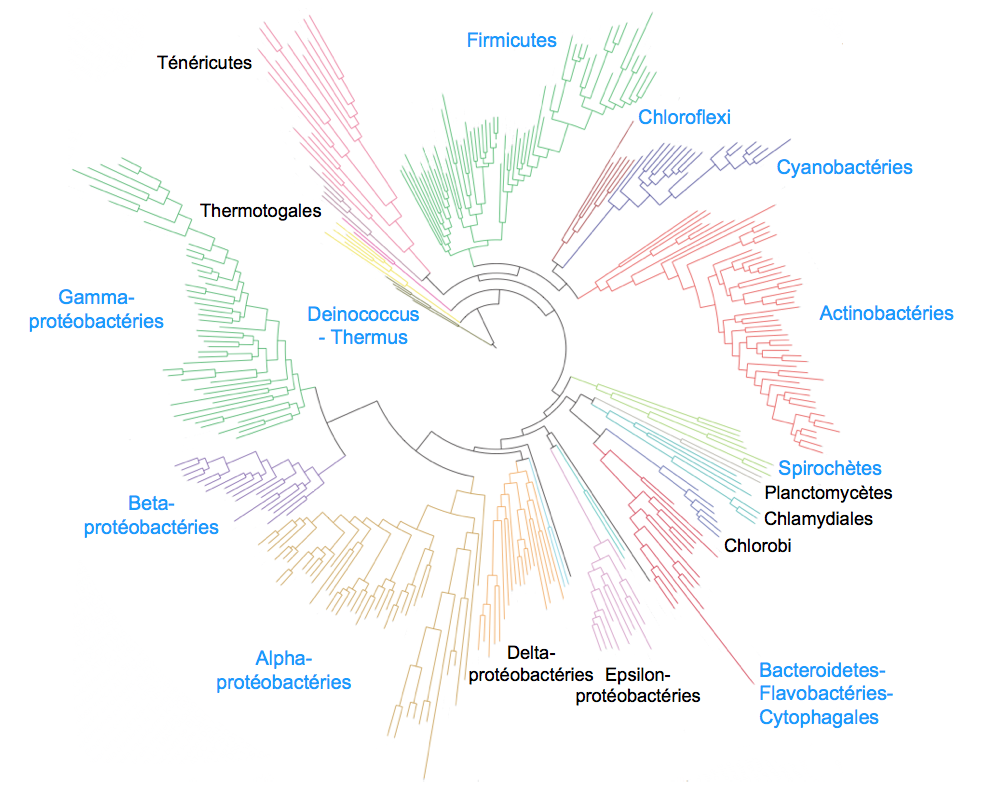
\includegraphics[height=0.4\textheight]{./img/figphylgeco.png}
	\caption[Distribution des génomes multipartites dans le domaine Bacteria]{Distribution des génomes multipartites (bleu) dans le domaine Bacteria.}\label{figphylgeco}
	 \end{center}
 \end{figure} 

	L'existence de RECE n'est pas corrélée avec la présence ou l'absence de plasmide au sein d'un génome. Ils peuvent être:
\begin{description}
      \item[$\bullet$] observés ponctuellement au sein d'une lignée (cas des Alteromonadales où seules deux espèces de \textit{Pseudoalteromonas} possèdent un génome multipartite,
      \item[$\bullet$] retrouvés chez un grand nombre d'espèces d'une même lignée sans être ubiquiste (cas des Rhizobiales où de nombreuses espèces (\textit{Brucella}, \textit{Ochrobactrum}, \textit{Rhizobium} et \textit{Sinorhizobium}), mais pas toutes (\textit{Bradyrhizobium}, \textit{Mesorhizobium}...) ont des génomes multipartites,
      \item[$\bullet$] ou encore présents dans toutes les espèces d'une lignée (cas des Vibrionales).
\end{description}
       La taille des RECE varie considérablement, le plus petit (0,27 Mb) étant trouvé chez \textit{Leptospira biflexa} et le plus grand  (3,7 Mb) chez \textit{Burkholderia gladioli}. Enfin, même si la majorité des RECE a une topologie circulaire, certains, dans les génomes de \textit{Agrobacterium} et de \textit{Cyanothece}, sont linéaires.\\
      Les espèces à génomes multipartites possèdent des écologies variées, pouvant être pathogènes (\textit{Brucella}, \textit{Vibrio}, \textit{Burkholderia}), des symbiotes de plantes (\textit{Burkholderia}, \textit{Rhizobium}) ou d'animaux (\textit{Vibrio}, \textit{Photobacterium}), avoir une écologie marine (\textit{Pseudoalteromonas}, \textit{Vibrio}, \textit{Anabaena}) ou être extrêmophiles (\textit{Deinococcus}), par exemple. 
     

\section{Essentialité}\label{chrIIess}
	L'essentialité d'un réplicon dépend directement de celle des gènes qu'il code. Ainsi, selon la définition d'Ochman \citep{Ochman2002}, un réplicon est considéré comme un chromosome s'il porte au moins un gène considéré comme essentiel à la vie de la bactérie, présent en copie unique dans le génome. La notion de gène essentiel pour un organisme relève du concept de ``génome minimal" où 100 à 300 gènes sont absolument indispensables à la survie et au développement de l'organisme bactérien \citep{Koonin2000,Glass2006}. Ces gènes codent majoritairement des protéines impliquées dans la réplication de l'ADN, la transcription des gènes, la traduction, et l'utilisation du carbone et de l'énergie \citep{MacLellan2004}. Le statut de chromosome s'applique ainsi au second réplicon de \textit{Rhodobacter sphaeroides} car il porte des gènes d'ARNr et de certaines enzymes du métabolisme primaire \citep{suwanto1989physical}. Le statut de chromosome a également été accordé aux réplicons de \textit{Butyrivibrio proteoclasticus} \citep{Kelly2010}, \textit{Nocardiopsis dassonvillei} \citep{Sun2010} et \textit{Ilyobacter polytropus} \citep{Sikorski2010}, car ils portent des gènes codant des ARNr et des ARN de transfert (\textbf{ARNt}). Le chromosome secondaire de \textit{Rhizobium radiobacter} (anciennement \textit{Agrobacterium tumefaciens}) possède la plupart des gènes codant des régulateurs transcriptionnels et des transporteurs ABC en plus de gènes d'ARNt et ARNr \citep{MacLellan2004}. De même, le second réplicon essentiel de \textit{Sinorhizobium meliloti} porte une part significative des gènes impliqués dans le métabolisme cellulaire et l'exploitation des sources de carbone et d'azote présentes au niveau du sol \citep{MacLellan2004}.\\
      La distinction entre chromosome et plasmide n'est cependant pas aussi tranchée et ne peut reposer sur la seule présence (chromosome) ou absence (plasmide) de gènes``marqueurs" sans copie sur un autre réplicon du genome. Certains réplicons plasmidiques portent des gènes essentiels \citep{Yeoman2011}, les plus fréquemment observés étant des opérons ARNr \citep{baril1992scattering,salanoubat2002genome,moran2004genome,pohlmann2006genome}. À l'inverse, il existe des RECE qui n'en codent pas \citep{Heidelberg2000,Nascimento2004}. Par ailleurs, de nombreux réplicons bien que plasmidiques contribuent significativement à la \textit{\textbf{fitness}} de leur hôte \citep{MacLellan2004,Krone2007,lopez2012rhizobial}, le terme \textit{fitness} désignant ici ce qui a rapport avec les capacités de survie et de développement d'un organisme bactérien à court, moyen et long terme, dans son (ou ses) habitat(s) naturel(s). Du fait de la difficile tâche de mesurer la contribution d'un gène ou d'un réplicon à la \textit{fitness} d'un organisme \citep{Mackenzie2004}, \textbf{il devient délicat de différencier chromosomes et plasmides uniquement sur la contribution d'un réplicon à la \textit{fitness} de l'organisme bactérien.} \\
      En règle générale, la distribution en gènes essentiels est largement déséquilibrée en faveur d'un réplicon principal (\textbf{chromosome primaire} ou \textbf{chr}) \citep{Mackenzie2004}, même si certains RECE font exception \citep{Choudhary2004,Egan2005,Choudhary2007}. Parmi les RECE recensés, on observe différents cas de figure (Tableau \ref{tabess}), empêchant l'inférence directe de règles quant à la distribution de gènes essentiels en nombre et type sur les RECE.   

\newpage

%%%%%%%%%%%%%%%%%%%%%%%%%%%%%%%%%%%%%%%%%%%%%%%%%%%%%%%%%%%%%%%%%%%%%%%%%
 \begin{longtable}{@{\hspace{-2cm}} >{\footnotesize\itshape}p{0.1\textwidth} | >{\small\flushleft}p{0.045\textwidth} | >{\small}p{0.04\textwidth} |>{\small}p{0.04\textwidth} | >{\footnotesize}p{0.6\textwidth} | >{\scriptsize}p{0.2\textwidth} @{\hspace{0.5cm}}}
    \endhead
	\caption[Caractéristiques essentielles des RECE]{Caractéristiques essentielles des RECE selon le genre de leur hôte.\\Source: génomes complets disponibles dans RefSeq au 23/11/2013. M: nombre de génomes multipartites rapporté au nombre total de génomes séquencés pour un genre bactérien donné. ARNr/ARNt: présence de gènes ARNr/ARNt. Référence: la première référence correspond à la première caractérisation du génome multipartite du genre quand elle est disponible, sinon les numéros d'accession des BioProjects (NCBI) sont fournis.}\label{tabess}\\
	  \multicolumn{1}{@{\hspace{-2cm}}l} {\small\textbf{Lignée}} & \multicolumn{1}{ l} {\small\textbf{M}}&\multicolumn{1}{ p{0.04\textwidth}} {\small\textbf{ARNt}}&\multicolumn{1}{ @{\hspace{0.3cm}}p{0.04\textwidth}@{\hspace{-0.3cm}}} {\small\textbf{ARNr}} & \multicolumn{1}{ c} {\small\textbf{Autres caractéristiques}} & \multicolumn{1}{ l} {\small\textbf{Références}}\\
	\endfirsthead
	\multicolumn{1}{@{\hspace{-2cm}}l}{\small\textbf{Lignée}} & \multicolumn{1}{ l} {\small\textbf{M}}&\multicolumn{1}{ p{0.04\textwidth}} {\small\textbf{ARNt}}&\multicolumn{1}{ @{\hspace{0.3cm}}p{0.04\textwidth}@{\hspace{-0.3cm}}} {\small\textbf{ARNr}} & \multicolumn{1}{ c} {\small\textbf{Autres caractéristiques}} & \multicolumn{1}{ l} {\small\textbf{Références}}\\
	\endhead
	\hline
	\multicolumn{1}{@{\hspace{-2cm}}} {} \\
	\multicolumn{1}{@{\hspace{-2cm}} p{0.15\textwidth}} {\textbf{Alphaprotéobactéries}}\\
	Agrobacterium & 4/4 & Oui & Oui & Présence de \textit{minCDE}, de gènes liés à la réplication de l'ADN, au métabolisme, à l'infection et de régulateurs transcriptionnels & \citep{wood2001genome,goodner2001genome,allardet1993presence},\citep{MacLellan2004,Slater2009} \\
	\hline
	Asticcacaulis & 1/1 & Oui & Oui & \centering - & PRJNA55641 \\
	\hline
	Brucella & 18/18 & Oui & Oui & Présence de l'opéron \textit{minCDE} et différents gènes d'ARNt-synthétases & \citep{Jumas-Bilak1998,paulsen2002brucella,delvecchio2002genome},\citep{MacLellan2004} \\
	\hline
	Ochrobactrum & 1/1 & Oui & Oui & Présence d'homologues de \textit{minC} et \textit{minD} & \citep{Slater2009,chain2011genome} \\
	\hline
	Paracoccus & 1/1 & Oui & Non & Présence de nombreux gènes d'ARNt-synthétases ou méthyltransférases & PRJNA58187 \\
	\hline
	Rhodobacter & 4/5 & Oui & Oui & Présence de nombreux gènes typiquement chromosomiques liés au métabolisme; Sous-représentation des gènes liés à la division cellulaire  & \citep{kiley1988molecular,suwanto1989physical,mackenzie2001home},\citep{Choudhary2004,Mackenzie2004,Mackenzie2007,Choudhary2007} \\
	 \hline
	Sinorhizobium & 1/1 & Non & Non & Présence de \textit{minCDE}, de gènes liés à l'infection et au métabolisme, et de régulateurs transcriptionnels; RECE similaire aux mégaplasmides des Rhizobiaceae  & \citep{kaneko2000complete},\citep{MacLellan2004,Slater2009} \\
	\hline
	Sphingobium & 2/2& Oui & Oui & Présence de gènes codant diverses enzymes essentielles, des sous-unités d'une ARN polymérase et des gènes impliqués dans le métabolisme et l'adaptation à l'environnement & \citep{nagata2010complete,Copley2012} \\
	\hline
	\multicolumn{1}{@{\hspace{-2cm}}} {}\\
	\multicolumn{1}{@{\hspace{-2cm}} p{0.15\textwidth}} {\textbf{Bêtaprotéobactéries}}\\
	Burkholderia & 39/40 & Oui & Oui & Présence de nombreux gènes impliqués dans le métabolisme primaire et la synthèse d'acides aminés; Répartition des gènes essentiels variable selon les espèces. Pour l\textit{B. cenocepacia}, ratio (chromosome/RECE-1/RECE-2) en gènes essentiels de l'ordre de 250/50/50 & \citep{Songsivilai2000,komatsu2003distribution,nierman2004structural},\citep{Guo2010} \\
	\hline
	Cupriavidus/ Ralstonia & 6/13 & Oui & Oui & Présence d'un gène d'une sous-unité de la polymérase et d'un facteur d'élongation avec des paralogues sur le chromosome. Présence de nombreux gènes impliqués dans l'infection des plantes et la formation du flagelle. & \citep{salanoubat2002genome},\citep{MacLellan2004,pohlmann2006genome,amadou2008genome} \\
	\hline
	Variovorax & 2/3 & Non & Oui & chromosome largement favorisé en gènes essentiels  & \citep{han2011complete} \\
	\hline
	\multicolumn{1}{@{\hspace{-2cm}}} {}\\
	\multicolumn{1}{@{\hspace{-2cm}} p{0.15\textwidth}} {\textbf{Gammaprotéobactéries}} \\
	Pseudo-alteromonas  & 2/3 & Non & Non & présence de gènes essentiels \textit{hisE} et \textit{gcpE}, ainsi que des gènes du métabolisme de l'histidine sur le RECE de \textit{P. haloplanktis}; génomes multipartites des deux espèces très similaires & \citep{medigue2005coping},\citep{Qin2011} \\
	\hline
	Vibrio  & 28/28 & Oui & Oui & Nombreux gènes impliqués dans la réparation de l'ADN, gènes impliqués dans le métabolisme énergétique, gènes de protéines ribosomales, d-sérine désaminase et thréonyl-tRNA synthétase; quasi majorité des gènes d'ARNr portée par le chromosome & \citep{trucksis1998vibrio,yamaichi1999physical},\citep{tagomori2002comparison,MacLellan2004,Heidelberg2000} \\
	\hline
	Aliivibrio  & 1/1& Oui & Oui & Génome proche du celui des \textit{Vibrio} & \citep{hjerde2008genome} \\
	\hline
	Photobacterium  & 1/1 & Oui & Oui & RECE en moyenne 25\% plus grand que ceux de \textit{Vibrio} & \citep{vezzi2005life} \\
     \hline
	\multicolumn{1}{@{\hspace{-2cm}}} {}\\
     \multicolumn{1}{@{\hspace{-2cm}} p{0.15\textwidth}} {\textbf{Acidobactéries}}\\
     Candidatus \textnormal{\mbox{Chloroacido-} \mbox{bacterium} \mbox{thermophilum}} & 1/1 & Non & Oui & Présence de gènes essentiels impliqués dans la chlorophototrophie & \citep{GarciaCostas2012}\\
	\hline
	\multicolumn{1}{@{\hspace{-2cm}}} {}\\
      \multicolumn{1}{@{\hspace{-2cm}} p{0.15\textwidth}} {\textbf{Actinobactéries}} \\
      Nocardiopsis & 1/1 & Oui & Oui & \centering - & \citep{Sun2010} \\
      \hline
	\multicolumn{1}{@{\hspace{-2cm}}} {}\\
      \multicolumn{1}{@{\hspace{-2cm}} p{0.15\textwidth}} {\textbf{Bacteroidetes}} \\
      Prevotella & 3/6 & Oui & Oui & \centering - & PRJNA47507, PRJNA51377, PRJNA65091, PRJNA163151\\
      \hline
	\multicolumn{1}{@{\hspace{-2cm}}} {}\\
      \multicolumn{1}{@{\hspace{-2cm}} p{0.15\textwidth}} {\textbf{Chloroflexi}}\\
      Sphaerobacter & 1/1 & Oui & Oui & \centering - &\citep{pati2010complete} \\
	\hline
	\multicolumn{1}{@{\hspace{-2cm}}} {}\\ 
	\multicolumn{1}{@{\hspace{-2cm}} p{0.15\textwidth}} {\textbf{Cyanobactéries}}\\
	Anabaena & 1/3 & Non & Oui & Présence de génes d'ARNt synthétases et ARNr méthyltransférases & \citep{Wang2012a} \\
	\hline
	Cyanothece & 1/6 & Non & Non& Présence de génes d'ARNt synthétases; Nombreux gènes singuliers du RECE linéaire & \citep{Welsh2008} \\
     \hline
     Thermobaculum & 1/1 & Non & Non & \centering - & \citep{Kiss2010} \\
     \hline
	\multicolumn{1}{@{\hspace{-2cm}}} {}\\
     \multicolumn{4}{@{\hspace{-2cm}} p{0.3\textwidth}} {\textbf{Deinococcus-Thermus}}\\
     Deinococcus & 1/7 & Oui & Oui & Présence de gènes d'ARNt synthétases; Nombreux gènes spécialisés dans l'adaptation à l'environnement & \citep{White1999}, \citep{MacLellan2004} \\
     \hline
	\multicolumn{1}{@{\hspace{-2cm}}} {}\\
     \multicolumn{1}{@{\hspace{-2cm}} p{0.15\textwidth}} {\textbf{Firmicutes}}\\
     Butyrivibiro & 1/2 & Oui & Oui & Présence des gènes essentiels \textit{acpD} et \textit{msrA}; gènes essentiels présents sur un plasmide de \textit{B. proteoclasticus} & \citep{Kelly2010},\citep{Yeoman2011} \\
     \hline
     Clostridium & 1/62 & Oui & Non & \centering - & DS,\citep{he2010evolutionary} \\
     \hline
	\multicolumn{1}{@{\hspace{-2cm}}} {}\\
      \multicolumn{1}{@{\hspace{-2cm}} p{0.15\textwidth}} {\textbf{Fusobactéries}}\\
      Ilyobacter & 1/1 & Oui & Oui & \centering - &\citep{Sikorski2010}\\
	\hline
	\multicolumn{1}{@{\hspace{-2cm}}} {}\\
	\multicolumn{1}{@{\hspace{-2cm}} p{0.15\textwidth}}{\textbf{Spirochètes}} \\
	Leptospira & 7/7 & Non & Non & Présence de \textit{ndh} (NADH déshydrogénase), \textit{gltB} (glutamate synthétase) et \textit{asd} (aspartate semialdéhyde dehydro-génase) & \citep{zuerner1993comparison,ren2003unique},\citep{Nascimento2004,bulach2006genome,Picardeau2008}\\
\end{longtable}
%%%%%%%%%%%%%%%%%%%%%%%%%%%%%%%%%%%%%%%%%%%%%%%%%%%%%%%%%%%%%%%%%%%%%%%%%

	Outre les RECE annotés, le statut de certains réplicons est ambigu. Bien que classés parmi les (méga)plasmides sur la base de caractéristiques structurales ou fonctionnelles, ils semblent jouer un rôle de RECE ou paraissent en posséder certaines caractéristiques. Ainsi, chez les Alphaprotéobactéries, différents plasmides de \textit{Rhizobium elti} (Rhizobiales) présentent de nombreuses caractéristiques (stabilité, essentialité...) de RECE \citep{Landeta2011}, ainsi que chez \textit{Azospirillum} (Rhodospirillales), bactéries promouvant la croissance de diverses plantes \citep{wisniewski2011azospirillum,Acosta-Cruz2012}. Différents plasmides des \textit{Roseobacter} seraient également des RECE sur la base de caractéristiques structurales (\textit{ori}, pourcentage en G+C) des réplicons \citep{Petersen2013}. 

\section{Régulation et intégration des RECE dans le cycle cellulaire}\label{model}
	La présence d'un chromosome additionnel dans un génome ajoute des contraintes à l'organisme et requiert des mécanismes moléculaires supplémentaires permettant son intégration dans le cycle cellulaire \citep{Venkova-Canova}. Par opposition à un plasmide, un RECE doit être répliqué une unique fois en un moment précis du cycle cellulaire et doit être activement ségrégé lors de la division cellulaire  \citep{Egan2005}.\\ 
	
Le modèle le plus populaire d'intégration d'un RECE dans le génome est l'adaptation des systèmes de réplication et ségrégation d'un mégaplasmide au cycle cellulaire \citep{Heidelberg2000,MacLellan2004}. Les mécanismes les mieux décrits sont ceux de \textit{V. cholerae} où l'hypothèse plasmidique d'origine du RECE est postulée \citep{egan2003distinct}. Il a été montré que le chromosome et le RECE de \textit{V. cholerae} se répliquent une fois par cycle cellulaire \citep{srivastava2007selective,stokke2011replication}. La réplication débute après celle du chromosome et termine en synchronisation avec lui \citep{rasmussen2007two,stokke2011replication}, et implique des régulateurs communs \citep{Egan2005,demarre2010dna}. Le RECE de \textit{V. cholerae} possède deux gènes spécifiques, \textit{rtcB} codant RtcB, protéine initiatrice de la réplication du RECE des \textit{Vibrionaceae} et \textit{Photobacteriaceae} à l'instar de DnaA pour la réplication du chromosome, et \textit{rtcA} intervenant dans la régulation de RctB \citep{duigou2006independent}. RtcB est de plus régulée par le chromosome par fixation à des motifs spécifiques localisés sur ce dernier \citep{baek2014chromosome}, ce qui démontre l'implication du chromosome dans la réplication du RECE et, partant, l'intégration du RECE dans le cycle cellulaire et le génome stable de \textit{V. cholerae}. La réplication du RECE est inhibée par une séquence adjacente à l'\textit{ori}, \textit{inc}, et semble aussi sous le contrôle de DnaA et Dam de par la présence de boîtes DnaA et de motifs GATC à l'origine \citep{egan2006autorepression,saint2008excess}. Interviennent également des mécanismes de \textit{handcuffing}, typiques des plasmides \citep{egan2003distinct,Egan2005,zakrzewska2007regulation}. Le RECE possède son propre système de partition ParA2/ParB2, essentiel à la maintenance du RECE, qui interagit (\textit{via} ParB2) avec \textit{rtcA} et RtcB, liant ainsi  réplication et ségrégation du RECE \citep{yamaichi2011regulatory}. Les mécanismes moléculaires de résolution de dimère de RECE font intervenir les mêmes résolvases XerC et XerD que pour le chromosome en le liant au cycle cellulaire par l'intermédiaire de l'action de FtsK \citep{Val2008}. FtsK est, pour le RECE comme pour le chromosome de \textit{V. cholerae} guidé par des motifs KOPS \citep{Val2008}.  \\

	 Le modèle de réplication/ségrégation de \textit{V. cholerae} met en évidence des adaptations génomiques spécifiques du RECE: présence de régulateurs et protéines supplémentaires spécifiques, motifs structuraux de régulation, qui semblent être le fruit de la modification d'un mégaplasmide chez l'ancêtre commun des \textit{Vibrio} \citep{Heidelberg2000}. Cependant, ce modèle est actuellement le seul décrivant en quelques détails les spécificités génomiques permettant l'intégration des RECE dans le cycle cellulaire, et ne peut \textit{de facto} être directement généralisé à tous les RECE.\\
	Les autres mécanismes d'intégration d'un réplicon additionnel dans le cycle cellulaire concernent principalement les spécificités de la partition chez les génomes multipartites des Burkholderiales, avec des adaptations des systèmes parABS des RECE en comparaison de ceux des chromosomes et des plasmides \citep{Dubarry2006a,Livny2007,Passot2012}. En particulier, ces adaptations impliquent une séquence \textit{parS} spécifique des RECE et une régulation des systèmes de partition des RECE de \textit{B. cenocepacia} par opposition à un système de partition plasmidique classique \citep{Dubarry2006a}.


\section{Origine évolutive}\label{chrIIori}
	Quelles sont donc les structures génétiques ancestrales expliquant la diversité actuelle des réplicons secondaires essentiels? D'un point de vue théorique, plusieurs hypothèses peuvent être envisagées:
	
\subsection*{Deux hypothèses sont principalement favorisées:}
\begin{description}
	 \item[H1] La scission chromosomique. Un unique réplicon se divise en plusieurs réplicons essentiels, faisant potentiellement intervenir des recombinaisons site-spécifiques (\textit{cf.} \S \ref{recom}). La coupure expérimentale d'un chromosome en deux molécules qui sont ensuite  transmises à la descendance a été décrite  \citep{guo2003natural,itaya1997experimental}. 
	 \item[H2]  L'adaptation d'un réplicon accessoire avec enrichissement progressif en gènes essentiels chromosomiques  \citep{Moreno1998,Mackenzie2004}. Cette hypothèse implique l'action de divers processus de recombinaisons génétiques entre chromosomes et plasmides, dont certains ont été identifiés et caractérisés \citep{Slater2009,Guo2010,maida2014origin}. Cette hypothèse est actuellement la plus généralement retenue pour rendre compte de l'existence de la plupart des génomes multipartites, en particulier de ceux des Protéobactéries \citep{Bavishi2010}. 
\end{description}
\subsection*{D'autres mécanismes ont été proposés:}
	 \begin{description}
	 \item[h1] Capture d'un chromosome externe \citep{Moreno1998,Mackenzie2004}. Il est alors nécessaire d'imaginer la formation d'une forme intermédiaire hybride, contenant plus d'un complément génomique.
	 \item[h2] Une réplication chromosomique inégale et/ou imparfaite faisant apparaître deux réplicons différents \citep{Moreno1998}, ce qui devrait se refléter dans la présence des régions dupliquées relativement abondantes dans le génome.
	 \item[h3]  Des mutations indépendantes sur des chromosomes d'espèces polyploïdes \citep{Moreno1998}, menant à une différentiation des chromosomes .
\end{description}

Même si les hypothèses h1, h2 et h3 sont vraisemblables, il n'existe pas à notre connaissance d'indice génomique indiscutable en leur faveur. Les hypothèses les plus susceptibles d'expliquer la formation des génomes multipartites les plus étudiés, avec les éléments les soutenant, sont synthétisés Table \ref{taborigin}.

%%%%%%%%%%%%%%%%%%%%%%%%%%%%%%%%%%%%%%%%%%%%%%%%%%%%%%%%%%%%%%%%%%%%%%%%%


\begin{longtable}{@{\hspace{-2cm}} >{\footnotesize\itshape}p{0.15\textwidth} | >{\bfseries\scriptsize}p{0.05\textwidth} | >{\scriptsize}p{0.50\textwidth} | >{\scriptsize}p{0.45\textwidth} @{\hspace{0.5cm}}}
	\caption[Origine évolutive des RECE d'après la littérature]{Origine évolutive des RECE d'après la littérature. \\ H: hypothèse(s) évolutive(s) des RECE.}\label{taborigin}\\
	\multicolumn{1}{@{\hspace{-2cm}} l} {\small\textbf{Lignée}} & \multicolumn{1}{p{0.03\textwidth}} {\small\textbf{Hyp}} & \multicolumn{1}{ @{\hspace{0.2cm}} l @{\hspace{-0.2cm}}} {\small\textbf{Origine de réplication}} & \multicolumn{1}{l} {\small\textbf{Autres caractéristiques}}\\
    \endfirsthead
		\multicolumn{1}{@{\hspace{-2cm}} l} {\small\textbf{Lignée}} & \multicolumn{1}{p{0.03\textwidth}} {\small\textbf{Hyp}} & \multicolumn{1}{ @{\hspace{0.2cm}} l @{\hspace{-0.2cm}}} {\small\textbf{Origine de réplication}} & \multicolumn{1}{l} {\small\textbf{Autres caractéristiques}}\\
     \endhead
     \hline
	\multicolumn{1}{@{\hspace{-2cm}}} {} \\
	\multicolumn{4}{@{\hspace{-2cm}} p{\textwidth}} {\textbf{Alphaprotéobactéries}}\\
	Asticcacaulis & ? & \multicolumn{2}{l}{\scriptsize Pas d'étude publiée de la structure génomique d'\textit{Asticcacaulis}}\\
	\hline
      Agrobacterium & H2 & Origine de réplication de type \textit{repABC} \citep{Slater2009} & Signatures génomiques proches de celles des plasmides;  ParA de type plasmidique \citep{MacLellan2004,Slater2009}.\\
     \hline
     
	Brucella & H2/ (H1/ h2/ h3) & Pour certains auteurs, l'\textit{ori} du RECE de \textit{B. melilentis} est similaire à celle du chromosome  \citep{delvecchio2002genome}, ce qui serait compatible avec les hypothèses H1,h2 et h3. Un locus \textit{repABC} est aussi présent \citep{MacLellan2004}; l'\textit{ori} du RECE  semble donc être homologue à celles de différents mégaplasmides et RECE de Rhizobiaceae \citep{paulsen2002brucella}. & Les ParA des RECE sont des homologues de protéines plasmidiques \citep{MacLellan2004} et de nombreux indices témoignent aussi d'un passé plasmidique proche de celui des autres mégaplasmides de la famille \citep{Slater2009}.\\
     \hline
      Ochrobactrum & H2 & Origine de réplication de type \textit{repABC} \citep{chain2011genome}. & Les génomes d'\textit{Ochrobactrum} et de \textit{Brucella} sont très proches phylogéniquement et génétiquement.\\
     \hline
	Paracoccus & ? & \centering - & Fréquents transferts entre les chromosomes et plasmides dans le genre \textit{Paracoccus} \citep{maj2013plasmids}. Certains plasmides des Rhodobacterales (dont fait partie \textit{Paracoccus}) possèdent des plasmides \textit{DnaA-like} caractéristiques \citep{petersen2011origin}\\
	\hline
	Rhodobacter & H1/ H2/ h2 & Présence d'un opéron \textit{repABC} \citep{Mackenzie2007} & Large duplication ancestrale entre le chromosome et le RECE \citep{Choudhary2004}. Expression génique faible  \citep{Mackenzie2007}. \\ 
	\hline
      Sinorhizobium & H2 & Origine de réplication de type \textit{repABC} \citep{barnett2001nucleotide,Slater2009} & RECE très proches des mégaplasmides des autres Rhizobiaceae \citep{Slater2009} \\
	\hline
      Sphingobium & H2 & Origine de réplication à proximité des gènes \textit{parA} et \textit{parB} ainsi que de \textit{repA} \citep{Copley2012} & Biais de distribution important des gènes essentiels en faveur du chromosome \citep{Copley2012}. \\ 
	\hline
	\multicolumn{1}{@{\hspace{-2cm}}} {} \\
	\multicolumn{4}{@{\hspace{-2cm}} p{\textwidth}} {\textbf{Bêtaprotéobactéries}}\\
	Burkholderia & H2 & Origine de réplication possédant des caractéristiques plasmidiques: proximité de \textit{parA} et \textit{parB}. Cependant: proximité de \textit{dnaG, polA} et \textit{rpoD} (transcription) absent du chromosome \citep{holden2004genomic} & Nombreux réarrangements et phénomènes de translocation intragénomique \citep{komatsu2003distribution,Guo2010}. Peu de gènes essentiels près des \textit{ori} des RECE \citep{Nagata2005}. Systèmes de partition \textit{parABS} \citep{morrow2012evolutionary,Passot2012,Dubarry2006a}\\
	Cupriavidus/ Ralstonia & H2 & \textit{ori} typique de mégaplasmide: proximité de \textit{repA} dont le produit est similaire à des protéines plasmidiques \citep{MacLellan2004,salanoubat2002genome} & De même que pour \textit{Burkholderia}, protéines parA homologues de protéines plasmidiques \citep{MacLellan2004,Passot2012}. \\
	\hline
	Variovorax & (H2)& L'origine de réplication n'a pas été identifiée dans le RECE \citep{han2011complete}& Distribution en gènes essentiels suggestive d'une origine de type H2 \citep{han2011complete}. \\
	\hline
	\multicolumn{1}{@{\hspace{-2cm}}} {} \\
	\multicolumn{4}{@{\hspace{-2cm}} p{\textwidth}} {\textbf{Gammaprotéobactéries}}\\
	Pseudo-alteromonas & H2 & Origine de réplication proche de celle du plasmide R1 \citep{medigue2005coping}. & La réplication serait unidirectionnelle \citep{medigue2005coping}.\\
	\hline
	Aliivibrio / Photobacterium/ Vibrio & H2 & \textit{ori} de type plasmidique malgré des caractéristiques uniques, présence de boîtes DnaA et motifs IHF, et mécanismes de régulation spécifiques chez \textit{V. cholerae} \citep{MacLellan2004}. Pas d'étude décrivant spécifiquement les \textit{ori} des \textit{Photobacterium} et \textit{Aliivibrio} & Protéine ParA proche des protéines plasmidiques \citep{Thompson2004}. Présence d'intégron typique des plasmides chez \textit{V. cholerae} \citep{Heidelberg2000}, mais pas chez les autres Vibrionaceae (intégron sur le chromosome). Des transferts entre le chromosome et le RECE ont été mis en évidence. Présence importante de transposases et transposons sur les RECE de \textit{P. profundum} et de \textit{A. salmonicida}  \citep{MacLellan2004,Kirkup2010,egan2003distinct,chen2003comparative} \\
     \hline
	\multicolumn{1}{@{\hspace{-2cm}}} {} \\
     \multicolumn{1}{@{\hspace{-2cm}} p{0.15\textwidth}} {\textbf{Acidobactéries}}\\
     Candidatus \textnormal{Chloroacido-bacterium thermophilum} & ? & \centering - & Distribution en gènes identique à celle du chromosome  \citep{GarciaCostas2012}. RECE plus sensible aux réarrangements génétiques que le chromosome \citep{GarciaCostas2012}. \\
	\hline
	\multicolumn{1}{@{\hspace{-2cm}}} {} \\
     \multicolumn{1}{@{\hspace{-2cm}} p{0.15\textwidth}} {\textbf{Actinobactéries}}\\
	Nocardiopsis & ? & \centering - & Le génome de \textit{N. alba} (non présent dans la base de données) a été séquencé et ne comporte qu'un unique chromosome \citep{qiao2012whole} \\
     \hline
	\multicolumn{1}{@{\hspace{-2cm}}} {} \\
     \multicolumn{1}{@{\hspace{-2cm}} p{0.15\textwidth}} {\textbf{Bacteroidetes}}\\
     Prevotella & ? & \centering - & Très grande diversité génomique au sein du genre \textit{Prevotella} \citep{Purushe2010}.\\
     \hline
	\multicolumn{1}{@{\hspace{-2cm}}} {} \\
     \multicolumn{1}{@{\hspace{-2cm}} p{0.15\textwidth}} {\textbf{Chloroflexi}}\\
     Sphaerobacter & ? & \centering - & \multicolumn{1}{c}{-} \\
     \hline
     Thermobaculum & ? & \centering - &\multicolumn{1}{c}{-}\\
     \hline
	\multicolumn{1}{@{\hspace{-2cm}}} {} \\
	\multicolumn{1}{@{\hspace{-2cm}} p{0.15\textwidth}} {\textbf{Cyanobactéries}}\\
	Cyanothece & ? & Les \textit{ori} n'ont pu être déterminées sur le chromosome ou le RECE par les méthodes de biais en GC \citep{Welsh2008}& RECE linéaire \\
	\hline
	Anabaena & ? & \centering - & Présence de gènes liés aux réplicases sur un plasmide \citep{kaneko2001complete}; Traces de prophages insérés \citep{Wang2012a}. Existence d'espèces à génome monopartite avec des plasmides similaires en taille au RECE \citep{kaneko2001complete}. \\
	\hline
	\multicolumn{1}{@{\hspace{-2cm}}} {} \\
     \multicolumn{1}{@{\hspace{-2cm}} p{0.15\textwidth}} {\textbf{Deinococcus-Thermus}}\\
     Deinococcus & H2/ (h3) & \textit{ori} à proximité de \textit{parAB}; gène \textit{rep} très similaire à un gène plasmidique \citep{MacLellan2004} & \textit{D. radiodurans} est typiquement polyploïde \citep{White1999}. Des ressemblances existent entre le RECE de \textit{D. radiodurans} et un mégaplasmide de \textit{Thermus thermophilus} \citep{omelchenko2005comparative} \\
     \hline
	\multicolumn{1}{@{\hspace{-2cm}}} {} \\
     \multicolumn{1}{@{\hspace{-2cm}} p{0.15\textwidth}} {\textbf{Firmicutes}}\\
     Butyrivibiro & H2 & \textit{ori} de type plasmidique \citep{Yeoman2011}. Un plasmide de \textit{B. proteoclasticus} possède de nombreuses protéines de la réplication de type chromosomique \citep{Yeoman2011} & très petit (0,3 Mb) \citep{Kelly2010} \\
     \hline
     Clostridium & ? & \centering - & \multicolumn{1}{c}{-}  \\
     \hline
	\multicolumn{1}{@{\hspace{-2cm}}} {} \\
     \multicolumn{1}{@{\hspace{-2cm}} p{0.15\textwidth}} {\textbf{Fusobactéries}}\\
     Ilyobacter & ? & \centering - & \multicolumn{1}{c}{-} \\
	\hline
	\multicolumn{1}{@{\hspace{-2cm}}} {} \\
	\multicolumn{1}{@{\hspace{-2cm}} p{0.15\textwidth}} {\textbf{Spirochètes}}\\
     Leptospira & H2 & Présence de boîtes DnaA à proximité de l'\textit{ori} \citep{ren2003unique}. Opéron de partition \textit{parAB} et gène \textit{rep} à proximité d'\textit{ori} \citep{Picardeau2008}. & Les caractéristiques génomiques  de \textit{Leptospira} suggèrent que le RECE (ainsi que certains plasmides) ont évolué à partir de prophages présents chez les Spirochètes \citep{Picardeau2008}.\\
\end{longtable}

%%%%%%%%%%%%%%%%%%%%%%%%%%%%%%%%%%%%%%%%%%%%%%%%%%%%%%%%%%%%%%%%%%%%%%%%%

	Concernant l'origine des différents génomes multipartites identifiés, on peut se demander si leur apparition est antérieure à celle de la lignée bactérienne (espèce, genre, famille les possédant ou si, au contraire, ces phénomènes sont récents et postérieur à l'émergence de la lignée (spéciation).\\ 
	La dispersion des génomes multipartites dans les différentes lignées bactériennes et à des niveaux variables de différentiation (espèce, genre, famille) suggère que \textbf{plusieurs apparitions indépendantes de génomes multipartites ont eu lieu au cours de l'évolution des génomes bactériens}. Ceci implique que l'émergence de génome multipartite est relativement ``facile" et s'effectue par l'action de mécanismes génétiques assez classiques. Il a été proposé que tous les RECE de Rhizobiaceae descendraient d'un réplicon extrachromosomique de type mégaplasmide, à réplication RepABC qui a capturé des gènes du chromosome, et dont des marqueurs géniques différents (\textit{minCDE, repABC}, par exemple) sont retrouvés dans chacune des lignées de Rhizobiaceae  \citep{Slater2009}. Alors que le mégaplasmide s'est intégré stablement dans le chromosome chez certaines espèces (\textit{Bradyrhizobium}), il a conservé son état de mégaplasmide chez d'autres ou bien a été tout simplement éliminé (\textit{Bartonella}) \citep{Slater2009}. Chez les  Vibrionales, les RECE semblent avoir coexisté avec le chromosome avant la diversification en différentes lignées, dont \textit{Vibrio, Aliivibrio, Photobacterium} et espèces de cette famille \citep{Thompson2004}. De même chez les Burkholderiales, l'analyse des systèmes \textit{parABS} \citep{Passot2012} met en évidence des similarités entre RECE et mégaplasmides des \textit{Burkholderia} et \textit{Ralstonia}, ce qui suggère un ancêtre commun plasmidique aux RECE de cette famille de bactéries. \textit{B. rhizixinica} fait cependant figure d'exception, son génome ne comportant qu'un seul chromosome et deux plasmides \citep{lackner2011complete}. Néanmoins, \textit{B. rhizixinica} en tant que pathogène endosymbiotique, possède un génome réduit et on peut faire l'hypothèse que cette espèce a opéré une réduction de son matériel génomique par un mécanisme similaire à celui décrit par Moreno \citep{Moreno1998} (\textit{cf.} paragraphe suivant). À l'inverse, les RECE présents chez \textit{Deinococcus, Clostridium, Prevotella, Anabaena, Cyanothece} et \textit{Rhodobacter} semblent être d'apparition relativement récente car des espèces du même genre ou de la même famille possédent un génome monopartite.

	
 \section{Rôle}\label{chrIIfunc}
	À ce jour, considérant la diversité d'organisation des génomes multipartites, il est difficile d'établir un rôle ou une fonction précise à cette architecture génomique. Il semble cependant improbable que l'organisation multi-chromosome du génome n'apporte aucun bénéfice à l'hôte, surtout si on postule que l'intégration et la stabilisation d'un second chromosome dans un génome représente un coût évolutif. Différentes tendances semblent se dessiner quant aux possibilités d'amélioration de la \textit{fitness} apportées à l'hôte par un génome multipartite. 
\begin{description}
	\item[$\blacktriangleright$]  Les RECE peuvent être des réservoirs de gènes accessoires, spécifiques d'un certain type d'écologie. Chez les  protéobactéries, les fonctions codées par les RECE sont majoritairement en lien avec des voies métaboliques spécifiques ou des mécanismes d'infection ou d'interaction avec différents hôtes \citep{galardini2013replicon}.
	\item[$\blacktriangleright$] Les RECE peuvent permettre une réplication plus rapide du génome ce qui est un avantage pour des espèces à taux de croissance élevé comme \textit{V. cholerae} en conditions favorables \citep{yamaichi1999physical}. Une réplication rapide peut aussi résulter par le lancement d'un cycle de réplication avant la fin du cycle cellulaire précédent \citep{stokke2011replication} comme chez \textit{Escherichia coli} \citep{skarstad1986timing}.
	\item[$\blacktriangleright$] Une structure du génome en plusieurs répliquons stables entraîne, lors de la réplication, une augmentation de l'expression génique par le phénomène de ``\textit{gene dosage}" pour les gènes proches d'\textit{ori} car dupliqués en premier  \citep{Jha2012}, à la fois au niveau du chromosome mais également du RECE. Cela permet de fournir rapidement et en grande quantité les protéines nécessaires au développement de la colonie, et pourrait apporter une nouvelle modalité de régulation de l'expression génique. 
	\item[$\blacktriangleright$] Chez \textit{Vibrio cholerae}, il a été suggéré que les deux chromosomes, dans certaines conditions, pourraient présenter une différence du nombre de copies, avec pour effet de moduler le niveau d'expression de certains gènes \citep{Heidelberg2000}. Un cas extrême serait la perte du chromosome ou du RECE qui conduirait à la formation de ``cellules drones" favorisant la survie de la population par un taux de sécrétion d'enzymes élevé \citep{Jha2012}.
	\item[$\blacktriangleright$] La perte du RECE a également été proposée comme mécanisme d'adaptation en réponse à des conditions environnementales défavorables dans le cas de \textit{Vibrio cholerae} \citep{Heidelberg2000}. Cependant, \textit{V. cholerae} n'est pas capable de survivre à plus d'un cycle cellulaire dans un tel cas \citep{yamaichi2007genes}. De plus, les chromosomes et RECE de \textit{V. cholerae} N16961 sont asservis l'un à l'autre par des systèmes Toxine-Antitoxine, entraînant la dégradation du chromosome en cas de perte du RECE \citep{yuan2011three}.
	\item[$\blacktriangleright$] Les génomes multipartites peuvent être une solution structurelle aux génomes de grande taille, long et difficile à se répliquer en un seul réplicon. Cependant l'existence de chromosomes bactériens de plus de 10 Mb prouve que la taille d'un génome ne peut seule expliquer la formation d'un RECE.
	\item[$\blacktriangleright$] Avoir un génome multipartite peut être un avantage par l'augmentation de la surface d'échange du génome avec le cytoplasme, ce qui permet, à taux d'échange constant, de réduire la taille des cellules et ainsi d'avoir une structure cellulaire plus adaptée à des environnements pauvres en nutriments \citep{morita1988bioavailability,stouthamer1993pays}.
	\item[$\blacktriangleright$] L'acquisition de gènes essentiels par un plasmide peut être vue comme un mécanisme (de type PSK) dans le sens où l'organisme ``solidifie sa relation" avec un plasmide qui apporte une contribution significative à l'augmentation de sa \textit{fitness} \citep{Slater2009}. 
	\item[$\blacktriangleright$] Les RECE semblent dans de nombreux cas être plus plastiques que les chromosomes. Ils présentent un taux global d'expression génique plus faible et/ou portent relativement moins de gènes et sont donc moins contraints sur le plan évolutif \citep{White1999,Choudhary2004}. Chez \textit{R. sphaeroides}, par exemple, les séquences des RECE sont plus divergentes que celles des chromosomes, ce qui semble indiquer une différence des vitesses d'évolution des deux réplicons \citep{Choudhary2007}. Cette différence peut s'expliquer par le fait que le RECE possède une expression génique plus faible que le chromosome, ainsi que des séquences intergéniques longues et serait donc plus enclin à subir des réarrangements génomiques fréquents. Les RECE peuvent ainsi servir d'``atelier évolutif" en étant des réservoirs des gènes à évolution rapide et moins exprimés, ou exprimés sporadiquement, ce qui est favorable aux bactéries dans certains milieux \citep{morrow2012evolutionary,Cooper2010,Bavishi2010,galardini2013replicon}.
	\item[$\blacktriangleright$] De plus, en facilitant les recombinaisons \textit{inter-} et \textit{intra}-chromosomiques, la structure multipartite peut participer à l'augmentation de la diversité des séquences \citep{Mackenzie2004}, à l'instar du phénomène décrit chez les Fungi \citep{Croll2012}.
	\item[$\blacktriangleright$] Enfin, chez les organismes endosymbiotes, un génome multipartite peut refléter un état de transition vers la réduction génomique dans lequel l'hôte se ``déleste"  d'une partie des gènes essentiels en les transférant à ses plasmides, qui sont éliminés par la suite \citep{Moreno1998}. \textit{Brucella} a été proposé comme exemple de cette configuration \citep{Wattam2009}.
\end{description}	

	La présence d'un état multipartite, conservé à travers le temps au cours de la diversification de différents groupes bactériens, reflète le succès évolutif de cette architecture génomique et son importance pour l'adaptation et l'évolution des organismes bactériens. Cela pourrait traduire des modalités d'évolution génomique spécifiques à certains milieux écologiques \citep{Slater2009}, comme par exemple dans les cas des Rhizobiaceae et des Burkholderiales où l'on observe de nombreux génomes multipartites et qui renferment une proportion importante d'espèces symbiotiques ou parasites des plantes. Cette architecture génomique pourrait aussi constituter une alternative efficace (ou neutre) à une structure classique monopartite du génome. Le cas de \textit{R. sphaeroides} illustre la dernière hypothèse: \textit{R. capsulatus} du même genre, possède un génome monopartite sans que cela semble être un avantage \citep{tichi2001interactive,Choudhary2007}. 
      
   
\section{Critères d'identification des RECE}\label{chrIIrece}
	Les propriétés caractéristiques des RECE sont:
\begin{itemize}
	\item[\textbf{- l'Essentialité}] Élément les distinguant fondamentalement des plasmides.
	\item[\textbf{- l'Intégration dans le cycle cellulaire}] impliquant une coordination avec le chromosome et une synchronisation avec la division cellulaire
	\item[\textbf{- Contribution à la \textit{fitness} de la bactérie}] d'une manière ou d'une autre la \textit{fitness}, sur le court ou long terme.
\end{itemize}
	Classiquement les RECE ont été majoritairement identifiés par leur caractère essentiel, notamment par la présence de gènes codant des ARNr et ARNt. Cependant la présence/absence de tels gènes est loin d'être suffisante pour classer un réplicon parmi les RECE.
	
	  

\subsection{Modèle du ``\textit{chromid}"}\label{parchromide}
	Récemment, l'appellation ``\textit{chromid}" a été introduite par Harrisson \textit{et al.} \citep{Harrison2010} pour décrire les RECE à partir du contenu en G+C et de la stratégie d'utilisation des codons synonymes (\textit{Relative Synonymous Codon Usage}; RSCU), le type d'origine de réplication, et les protéines ParA/B \citep{harrison2011bacterial}, et a depuis été reprise par plusieurs auteurs lors d'études ponctuelles de génomes de protéobactéries \citep{maj2013plasmids,Acosta-Cruz2012,Petersen2013,galardini2013replicon,Ramirez-Bahena2014,wisniewski2011azospirillum}.
	
	 Selon ce modèle:
\begin{description}
	\item[$\bullet$] Les \textit{chromid} possèdent des systèmes de réplication et de maintenance proches de ceux des plasmides.
	\item[$\bullet$] Les \textit{chromid} ont des compositions en G+C et RSCU proches de ceux des chromosomes (et relativement plus que des plasmides) ce qui suggère qu'ils ont co-habité avec le chromosome pendant relativement plus longtemps que ne le font des plasmides classiques \citep[Fig. 1]{Harrison2010}. 
     \item[$\bullet$] Les \textit{chromid} portent des gènes essentiels, mais aucun des 284 gènes identifiés du génome-coeur n'est présent sur les \textit{chromid} de \textit{Burkholderia} étudiés \citep{harrison2011bacterial}. Ils portent de plus de nombreux gènes accessoires (relativement plus que les chromosomes), qui sont conservés au sein d'un genre bactérien.  
\end{description}

	Les gènes communs à l'ensemble des membres de la famille bactérienne (Burkholdériales) étudiée par Harrison \textit{et al.} sont relativement conservés alors qu'ils ne le sont que faiblement quand ne sont considérés qu'un genre (\textit{Burkholderia}) ou qu'une espèce (\textit{B. cenocepacia}), indiquant une plasticité des RECE accrue par rapport aux chromosomes dans les génomes étudiés \citep[Fig. 2]{Harrison2010}. Enfin, l'ordre des gènes sur les \textit{chromid} est très peu conservé en comparaison des chromosomes à des niveaux taxonomiques supérieurs au genre  \citep{harrison2011bacterial}. Ces constatations rejoignent les résultats des travaux de Bavishi \textit{et al.} \citep{Bavishi2010} où les longueurs relatives des alignements significatifs des RECE sont comparées à celles des chromosomes pour les génomes de souches de la même espèce ou d'espèces différentes, ce qui suggère une différence de vitesse d'évolution entre chromosomes et RECE \citep{Bavishi2010}. 
    
    
\subsection{Autres modèles}\label{parmodelepl}
	Plusieurs études ont tenté de classer les différents types de plasmides et réplicons accessoires. Des critères structurels comme la présence de complexe de mobilisation/conjugaison ainsi que les caractéristiques des différentes relaxases peuvent servir pour discriminer les réplicons accessoires \citep{garcillan2009diversity}. Il est cependant à souligner que les RECE, par leur rôle positif probable sur la \textit{fitness} de la bactérie, n'ont pas besoin de système de maintenance ``égoïste" de type plasmidique \citep{Smillie2010}. D'autres travaux proposent de classer les plasmides selon les gènes des modules de réplication \citep{jensen2010classification,Petersen2011}. Ces approches peuvent dans un premier temps sembler pertinentes pour la caractérisation des RECE, ceux-ci adaptant potentiellement ces protéines afin de s'intégrer dans le cycle cellulaire. Cependant, ces études se focalisent sur un gène ou opéron (\textit{repABC)} unique et ne prennent pas en compte les mécanismes intervenant dans la ségrégation et la maintenance des RECE. 
   


\section{Données génomiques de notre étude}   
	La question se posant naturellement à propos de la structure spécifique des réplicons secondaires essentiels est: \textbf{Existe-il des gènes, ou distributions de gènes, communs à l'ensemble de ces réplicons?} Différents éléments de réponse, abordés dans ce chapitre montrent qu'il n'existe pas de règle de fixation d'un gène, ou groupe de gènes, particulier sur les réplicons secondaires accessoires permettant d'expliquer leur transformation en réplicon essentiel. Les analyses des chapitres suivants ont donc pour objectif de caractériser d'éventuels biais de répartition de gènes des STIG à partir de l'analyse de l'intégralité des séquences complètes des génomes bactériens multipartites référencés dans \textbf{RefSeq} \citep{pruitt2007ncbi} à la date du 23/11/2013 (\textit{c.f.} Annexe \ref{AppendiceA}). \\
       Notre jeu de données comprend 2016 génomes bactériens et 1267 plasmides isolés, soit 2016 chromosomes, 2781 plasmides et 129 RECE selon les annotations de RefSeq. Les distributions de la taille et du nombre de gènes (les deux étant hautement corrélés) présents sur les réplicons bactériens (Figure \ref{figsize}) met en évidence de nettes différences entre RECE, plasmides et chromosomes primaires. 

\begin{figure}[H]
	\hspace{-2cm}
	\begin{subfigure}{0.6\textwidth}
		\centering
		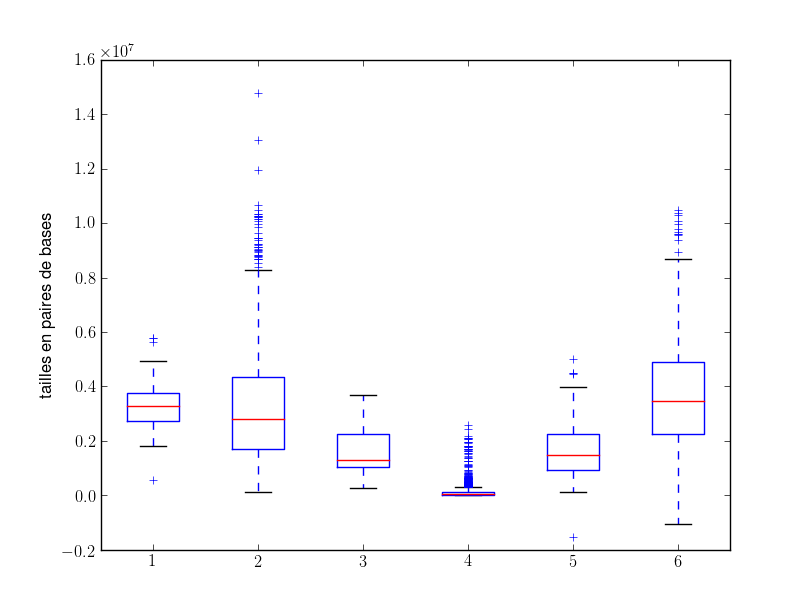
\includegraphics[width=0.9\textwidth]{./img/replicon_mustach.png}
		\caption{Tailles des génomes}\label{taille}
	\end{subfigure}
	\begin{subfigure}{0.6\textwidth}
		\centering
		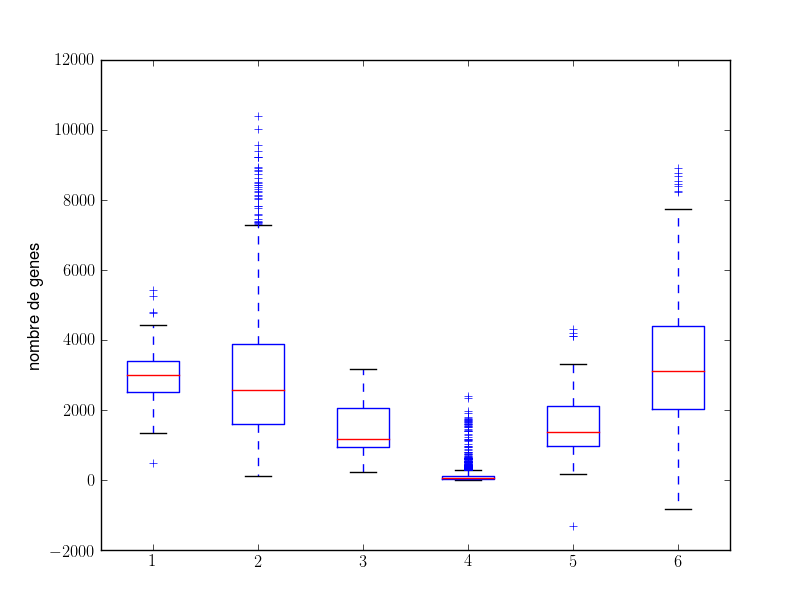
\includegraphics[width=0.9\textwidth]{./img/gene_mustach.png}
		\caption{Nombre de gènes}\label{nbgene}
	\end{subfigure}
	\caption[Distributions des tailles et nombres de gènes des réplicons]{Distributions des tailles (\ref{taille}) et nombres (\ref{nbgene}) de gènes des réplicons. \\
	Les boites délimitent les premiers et troisièmes quartiles (Q) des distributions, les limites des ``moustaches" inférieures et supérieures représentant respectivement Q1-1.5(Q3-Q1) et Q3+1.5(Q3-Q1). Les points en dehors des moustaches sont représentés par des croix. \textbf{1}: chromosomes des génomes multipartites. \textbf{2}: totalité des chromosomes. \textbf{3}: RECE. \textbf{4}: plasmides. \textbf{5}: différences des tailles (\ref{taille}) ou nombres de gènes (\ref{nbgene}) entre chromosome et RECE au sein d'un génome. \textbf{6}: différences des tailles (\ref{taille}) ou nombres de gènes (\ref{nbgene}) entre chromosome et plasmide au sein d'un génome.}\label{figsize}
\end{figure} 
	Ces facteurs ne sont pas suffisants pour caractériser les différents réplicons: Il existe des plasmides aussi grands que des RECE, et des RECE aussi grands que des chromosomes. Enfin, la répartition très inégale des génomes multipartites dans les différents groupes et genres bactériens (Figure \ref{specieplot}), pour des raisons évolutives ou historiques, crée un biais dans les données, biais dont il faudra tenir compte dans l'analyse.
\newpage
\usepgfplotslibrary{units}

\thispagestyle{empty}
\begin{figure}[H]
	\vspace{-2.5cm}	
      	\hspace{-2cm}
      	\begin{subfigure}{0.55\textwidth}
      		\begin{tikzpicture}
      		\tikzstyle{every node}=[font=\small]
\pie[cloud,scale font,sum=auto, color={purple!40,pink!60,magenta!80,red!60,cyan!60,blue!60,blue!40,green!10,lime!40,green!40,purple!1,black!20}]{1/,1/,2/,2/,2/,1/,2/,34/,47/,32/,7/,1/}
      		\end{tikzpicture}
      		\subcaption{Répartition des génomes multipartites à travers le domaine bactérien. Total:\textbf{133}}\label{fig1}
      \end{subfigure}
      \hspace{1cm}
      \begin{subfigure}{0.55\textwidth}
      	\begin{tikzpicture}
      	\tikzstyle{every node}=[font=\small]
      	\pie[cloud,scale font,sum=auto,color={purple!40,pink!60,magenta!80,red!60,cyan!60,blue!60,blue!40,green!10,lime!40,green!40,purple!1,black!20}]{1/,1/,1/,2/,2/,1/,2/,10/,4/,5/,1/,1/}
      	\end{tikzpicture}
       \subcaption{Répartition des genres bactériens ayant au moins un génome multipartite. Total:\textbf{31}}\label{diversite}
	 \end{subfigure}
      \\
      \\
      \vspace{1cm}
      \hspace{-4cm}
      \begin{subfigure}{1\textwidth}
      	\begin{tikzpicture}
      	\tikzstyle{every node}=[font=\small]
      	\pie[cloud,scale font,sum=auto,color={purple!40,pink!60,magenta!80,orange!40,red!60,cyan!60,blue!60,blue!40,green!10,lime!40,black!10,green!1,green!40,purple!1,brown!20,black!20}]{8/,345/,111/,110/,19/,82/,23/,745/,280/,168/,61/,109/,714/,82/,89/,104/}

      	\end{tikzpicture}
     {\advance\leftskip+3cm\subcaption{Répartition des génomes bactériens disponibles. Total:\textbf{3052}}}
    	\end{subfigure}
	\begin{subfigure}{1\textwidth}\label{fig2}
	\hspace{-3cm}
      	\begin{tikzpicture}
      	\tikzstyle{every node}=[font=\small]
      	\pie[cloud,scale font,sum=auto,text=legend,color={purple!40,pink!60,magenta!80,orange!40,red!60,cyan!60,blue!60,blue!40,green!10,lime!40,black!10,green!1,green!40,purple!1,brown!20,black!20}]{6/Acidobactéries,79/Actinobactéries,61/Bacteroidetes,6/Chlamydiae,11/Chloroflexi,34/Cyanobactéries,6/Deinococcus-Thermus,90/Firmicutes,72/Alphaprotéobactéries,49/Bêtaprotéobactéries,29/Deltaprotéobactéries,11/Epsilonprotéobactéries,104/Gammaprotéobactéries,9/Spirochètes,6/Ténéricutes,69/autres}

      	\end{tikzpicture}
      {\advance\leftskip+3cm\caption{Répartition des genres bactériens ayant au moins un génome disponible. Total:\textbf{638}}}
      \end{subfigure}
      \hspace*{-3cm}
      \begin{minipage}{1.37\textwidth}
      \medskip
      \caption[Répartition par lignée des génomes bactériens disponibles]{\scriptsize Répartition par lignée des génomes bactériens disponibles au 23/11/2013 dans la base de données RefSeq \citep{pruitt2007ncbi} classés selon la taxonomie bactérienne en vigueur (http://www.bacterio.net/).\\
       Seuls les génomes complets ont été pris en compte. Les génomes sont organisés selon le phylum de leur hôte sauf pour les Protéobactéries pour lesquels la classe a été utilisée. La catégorie ``Autres" regroupe les phylum faiblement représentés dans RefSeq: Aquificae, Chlorobi, Deferribacteres, Fibrobacteres, Fusobactéries, Gemmatimonadetes, Nitrospirae, Planctomycètes, Thermodesulfobactéries, Thermotogae, et Verrucomicrobia.}\label{specieplot}
       \end{minipage}       
\end{figure}


\section{Nature, origine et fonctionnement des RECE: une problématique ouverte}\label{justification}    
	
Jusqu'à maintenant, la problématique de ce que sont les RECE a été abordée principalement au cours d'études ponctuelles de génomes individuels et parfois, d'espèces bactériennes. Plusieurs tentatives de définition ont été faites \citep{Mackenzie2004}, la plus complète et récente étant celle de Harrison \citep{harrison2011bacterial}, sans pour autant clôturer le débat sur la nature chromosomique \textit{vs.} plasmidique des RECE. En effet, l'étude de Harrison ne s'attache qu'à la comparaison des RECE aux chromosome et plasmide(s) présents dans le même génome, et est majoritairement focalisée pour ce qui est de l'étude approfondie, sur une seule espèce
 (\textit{Burkholderia cenocepacia}) d'un seul genre (\textit{Burkholderia}) d'une seul famille (Burkholderiaceae). Ces résultats ne peuvent donc pas être directement généralisés à l'ensemble des RECE bactériens. Les travaux de Harrison \textit{et al.} \citep{Harrison2010, harrison2011bacterial} apportent néanmoins de précieuses observations, dont l'interprétation va au-delà de l'introduction de l'appellation de ``\textit{chromid}". En effet, la définition du \textit{chromid} revient à dire que les RECE fonctionnent comme des chromosomes mais ne peuvent être appelés chromosome parce qu'ils sont plasmidiques à l'origine. La question devient alors : \textbf{Qu'est-ce qu'un chromosome?} \\
	Les différents éléments présentés dans ces deux premiers chapitres mettent en évidence une continuité génomique entre plasmides, RECE et chromosomes, et révélent l'existence de mécanismes moléculaires et structures génomiques communs à ces différents types de réplicons. Cette similitude est d'autant plus affirmée qu'il devient difficile de discerner si certains réplicons sont des (méga)plasmides ou des chromosomes. Ainsi la définition même de RECE n'est pas appropriée, la distinction entre réplicons bactériens pouvant au final se résumer à deux éléments: leur essentialité pour l'organisme les hébergeant et leurs intégration et stabilisation dans le cycle cellulaire, leur rôle en étant une conséquence. Du point de vue de l'évolution du matériel génétique, les bactéries à génome multipartite représentent de fait une collection de données génomiques cruciale pour appréhender les nature et importance des forces évolutives mises en œuvre dans l'organisation du matériel génétique et la complexification et l'adaptation des génomes bactériens. Or, les études faites jusqu'à présent ne permettent pas de caractériser clairement et de manière générale ce que sont un plasmide, un chromosome ou un RECE parmi les réplicons bactériens. \\
       Les travaux de cette thèse portent sur la caractérisation des génomes multipartites par une \textbf{étude globale sans \textit{a priori} de l'ensemble des génomes bactériens et données disponibles dans les bases de données publiques} dont l'objectif est d'identifier des tendances générales des mécanismes génétiques impliqués dans l'apparition et la stabilisation des architectures génomiques multipartites. 























    
\chapter{Stratégie d'étude}\label{chap2}
\lhead{\emph{Stratégie d'étude}}


Les \textbf{S}ystèmes de \textbf{T}ransmission de l'\textbf{I}nformation \textbf{G}énétique (\textbf{STIG}) sont les mécanismes génétiques permettant la réplication, la ségrégation et la maintenance des réplicons au cours des générations. {\color{orange}\bf Le passage d'un génome monopartite à multipartite (ou inversement) doit logiquement passer par une adaptation des STIG du génome afin de permettre l'intégration de la réplication et de la ségrégation d'un chromosome additionnel (ou sa disparition) dans le cycle cellulaire et vis-à-vis de chromosomes préexistants}. Il apparaît alors pertinent de caractériser les réplicons et génomes bactériens selon les STIG qu'ils utilisent. Dans cette étude, nous recherchons plus spécifiquement à mettre en contraste les RECE par rapport aux chromosomes primaires (et chromosomes uniques) et aux “vrais” plasmides afin, premièrement, de discriminer efficacement les différentes catégories de réplicons et secondairement, d'identifier les systèmes-clés de l'émergence et de la stabilisation des génomes multipartites. 

\section{Les protéines des STIG: variables explicatives des réplicons}\label{parchap2introworkflow}
Les chapitres \ref{chap1a} et \ref{chap1b} ont présenté les STIG des réplicons bactériens, ainsi que la conception actuelle de l'architecture du génome bactérien. Il semble alors que les types de réplicon, et les espèces et écologies des organismes les hébergeant sont fonctionnellement liés à leurs STIG. \textbf{Selon notre postulat d'adaptation des STIG dans les génomes multipartites, des différences de distribution des gènes liés aux STIG entre génome mono- et multi-partites doivent être détectables par une analyse bioinformatique}. Nos données de départ étant l'ensemble des génomes bactériens séquencés disponibles dans les bases de données publiques, nous annotons dans un premier temps l'ensemble des gènes liés aux STIG dans ces génomes. En prenant ces gènes comme attributs des réplicons, nous analysons ensuite ce jeu de données pour identifier et caractériser d'éventuels biais de distribution entre les réplicons, afin, à partir de ces résultats, de distinguer les différents types de réplicons. Enfin, nous relions ces biais à des réalités biologiques et génomiques.
Deux types d'attributs sont utilisés pour caractériser les réplicons bactériens:
\begin{description}
\item[\textbullet]les groupes d'homologues des protéines liées au STIG, 
\item[\textbullet]les différentes fonctions de ces protéines.
\end{description}
Dans le premier cas, la mesure rapprochant deux protéines étant l'homologie de séquence, la proximité de deux réplicons traduira un lien évolutif potentiel. Dans le second cas, les réplicons seront identifiés selon leur fonctionnalité.

\section{Fondement de la génomique comparative}\label{introchap2}
Trois modalités d'analyse bioinformatique peuvent être distinguées:
\begin{itemize}
\item L'analyse de séquences biologiques (protéines, ARN, ADN), “analyse” sous-entendant la comparaison (recherche d'homologie) des séquences. 
\item La modélisation moléculaire qui consiste à inférer le comportement et/ou l'organisation de structures moléculaires.
\item La biologie des systèmes, cherchant à construire des modèles reliant différents niveaux d'information biologique (structural, moléculaire, écologique...).
\end{itemize}
\medskip
Un des paradigme fondamental est que l'\textbf{homologie} de séquence est liée à une origine évolutive commune des séquences comparées \citep{wray1998homology} et, à un degré moindre, à une \textbf{homologie fonctionnelle} \citep{chikina2011accurate}. Ces hypothèses permettent, par exemple, d'étudier les relations phylogéniques entre individus ou d'annoter une séquence biologique inconnue par rapport à des séquences biologiques déjà annotées.\\
L'homologie de deux séquences peut refléter différents mécanismes évolutifs:
\begin{description}
\item[$\bullet$ \textbf{Orthologie}] \citep{fitch1970distinguishing} Deux séquences chez deux organismes distincts sont orthologues si elles descendent d'une unique séquence ancestrale présente dans le dernier ancêtre commun aux deux espèces. L'homologie de deux gènes séparés par un événement de spéciation laisse supposer que les gènes ont conservé la fonction du gène ancestral et ont, \textit{a priori}, la même fonction.
\begin{figure}[H]
\Tree [.{\hspace{1cm}Gène $\alpha$ ancestral $\Longleftarrow\mathrm{\textbf{Spéciation}}$} {Gène $\alpha$ Espèce A} {Gène $\alpha$ Espèce B} ]
\subcaption{\textbf{Orthologie} entre les gènes $\alpha$ des espèces A et B.}\label{figrotho}
\end{figure}
\item[$\bullet$ \textbf{Paralogie}] \citep{fitch1970distinguishing} Deux g sont paralogues si elles résultent d'une \textbf{duplication génique}. On distingue de plus les \textbf{In-paralogues} si la duplication a eu lieu avant l'événement de spéciation, et les \textbf{Out-paralogues} si la duplication a eu lieu après la spéciation.
\begin{figure}[H]
\hspace{-1.5cm}
\begin{minipage}{0.5\textwidth}
\Tree [.{\hspace{1cm}Gène $\alpha$ ancestral $\Longleftarrow\mathrm{\textbf{Duplication}}$} {Gène $\alpha$ Espèce A} {Gène $\beta$ Espèce A} ]
\subcaption{\textbf{In-paralogie} entre les gènes $\alpha$ et $\beta$ de A.}\label{figinpara}
\end{minipage}
\begin{minipage}{0.5\textwidth}
\Tree [.{\hspace{1cm}Gène $\alpha$ ancestral $\Longleftarrow\mathrm{\textbf{Spéciation}}$} {Gène $\alpha$ Espèce A} [.{Gène $\alpha$ Espèce B $ \Longleftarrow\mathrm{\textbf{Duplication}}$} {Gène $\alpha$ Espèce B} {Gène $\beta$ Espèce B} ] ]\\
\subcaption{\textbf{Out-paralogie} entre le gène $\alpha$ de A et le gène $\beta$ de B.}\label{figoutpara}
\end{minipage}
\end{figure} 
\medskip
La duplication génique est souvent suivie d'une divergence fonctionnelle des gènes dupliqués. Un des gènes conserve la fonction du gène ancestral et l'autre diverge pour acquérir une nouvelle fonction \citep{fitch1970distinguishing,fitch2000homology}. 
\item[$\bullet$ \textbf{Xénologie}] Deux gènes sont xénologues si leur homologie traduit une histoire évolutive commune mais, pour l'une des espèces les hébergeant, n'est pas liée au gène présent dans l'ancêtre direct dont ces dernières sont issues. Dans les génomes bactériens, la présence de séquences xénologues témoigne fréquemment d'un transfert horizontal de gènes (THG) inter-réplicons et/ou inter-individus. L'évolution des génomes bactériens étant soumise à un flux important de THG (\citep{Bapteste2009,Doolittle2007}), la détection d'orthologues au sein des différents réplicons est souvent délicate et bruitée par les xénologues.
\end{description} 


\section{Concept du génome-cœur}\label{coregenome}
De nombreuses études mettent en avant la présence d'une collection de gènes homologues chez l'ensemble des membres d'une espèce (par exemple, pour \textit{Salmonella enterica} \citep{lan2009population} ou \textit{Helicobacter pylori}). Cela a conduit à la proposition de l'hypothèse du \textbf{génome-cœur} ou \textit{Core Genome Hypothesis} \citep{lan1996gene}. Cette théorie distingue la fraction du génome (le cœur) partagée par tous les membres de l'espèce, de la fraction auxiliaire qui est seulement présente dans une sous-population. Le génome-cœur définit ainsi les spécificités d'une espèce bactérienne. Les gènes du génome-cœur codent principalement les fonctions métaboliques essentielles et les processus cellulaires de transmission d'information \citep{Riley2009}. Ainsi, \textbf{une part importante des gènes des STIG sont inclus dans le génome-coeur des bactéries}. Les génes de la partie auxiliaire sont principalement les gènes codant des fonctions métaboliques supplémentaires, utiles dans le contexte de certaines écologies, et sont plus fréquemment associés à des plasmides ou des éléments mobiles \citep{Riley2009}.
\iffalse
single gene/motif detection: \citep{Brilli2010}.
TGH: \citep{Bosi2011}.
Association rules pour clustering et visualisation de données biologiques \citep{Karpinets2012}.
Phylogénomique: Besoin moderne de phylogénie \citep{chan2013next}.
Remote homologie detection \citep{Bernardes2011}.
Protéines organisées en domaines: Une combinaison de domaines similaires, témoigne-t-elle d'une même fonction, d'une origine commune ou est-elle due au hasard? \citep{song2008sequence}.
Théorie du core genome hypothesis? 
\fi

\section{Fouille de données en génomique}\label{analyseintro}

\subsection{Méthodes analytiques}
Avec l'explosion de la production de données génomiques, et en particulier l'avènement de nouvelles technologies de séquençage de l'ADN et des méthodes \textit{chip-seq}, les chercheurs sont confrontés à un afflux massif de données génomiques, transcriptomiques, protéomiques ou physiologiques. Cette avalanche de données est devenue un défit pour les bio-analystes et requiert le développement constant de méthodes analytiques permettant de traiter de façon pertinente (et de stocker) des quantités toujours plus importantes d'information génétique bruitée dans des temps raisonnables.\\
Les données à analyser sont souvent multivariées, \textit{i.e.}, décrites par une collection de paramètres (taux d'expression génique, présence/absence de gènes, écologie des organismes ...) généralement considérés comme des variables aléatoires. Parmi les méthodes d'analyse multivariée, on distingue les méthodes de statistiques classiques, impliquant des tests d'hypothèses, des méthodes dites de fouille de données (\textit{\textbf{data mining}}) généralement employées pour analyser des jeux de données massifs et multi-dimensionnels \citep{izenman2008modern}. Le terme \textit{data-mining} fait référence à un concept un peu “fourre-tout” englobant des approches de transformation et de préparation des données, de visualisation, d'extraction de connaissance et d'évaluation. Parmi ces méthodes d'analyses, nous pouvons distinguer les \textbf{méthodes descriptives}, qui ont pour objectif d'explorer les données (recherche d'observations aberrantes (\textbf{\textit{outliers}}), de structures ou de tendances, sélection de variables...), des \textbf{méthodes prédictives} où l'objectif est de construire un modèle à partir des données. Les méthodes de data-mining ont souvent recourt à des concepts statistiques, mais une part importante de ces méthodes englobe les approches dites d'apprentissage (\textbf{\textit{Machine Learning}}). À partir d'un jeu de données, les algorithmes prédictifs de machine learning cherchent à apprendre, à reconnaître des tendances complexes et sont capables de prendre des “décisions”' en fonction des données \citep{han2012data}. Une façon de conceptualiser les problèmes d'apprentissage est d'imaginer qu'est recherché à travers un espace de concepts descriptifs, un ensemble de règles décrivant au mieux un jeu de données \citep{witten2013data}. Ainsi, un algorithme de machine learning est défini par les différents concepts descriptifs utilisés pour représenter les données, l'ordre dans lequel est parcouru l'espace des concepts et la façon dont sont traités les problèmes de sur-apprentissage (ou \textbf{\textit{overfitting}}) des jeux de données d’entraînement (\textbf{\textit{training set}}) \citep{witten2013data}. Enfin, nous pouvons distinguer les méthodes d'\textbf{apprentissage supervisé} (classification ou régression), où un ensemble de variables d'entrée (\textbf{\textit{input}}) dont l'état de sortie (\textit{\textbf{output}}) est connu sert à entraîner un algorithme d'apprentissage afin de traiter des données dont l'état de sortie n'est pas connu, des méthodes d'\textbf{apprentissage non-supervisé} (clustering par exemple) où aucune information \textit{a priori} n'est disponible sur l'état de sortie des données. \\
\\
L'efficacité d'un algorithme peut être mesurée selon différents critères. Dans l'analyse de données biologiques, on peut souligner l'importance de: 
\begin{description}
\item[$\bullet$] \textbf{La complexité temporelle et spatiale}, c'est-à-dire la faisabilité temporelle et matérielle d'un algorithme. Cela ce traduit concrètement par le temps d'exécution d'un algorithme $t$, et la taille de la mémoire nécessaire $m$. Formellement les complexités temporelle et spatiale peuvent être représentées par des fonctions $O_{t}(Y)$ et $O_{m}(Y)$ indiquant que $t$ et $m$ vont être proportionnels à $Y$, où $Y$ s'exprime généralement en fonction du nombre de données à analyser $n$, et de la dimension des données $d$ ($Y=f(n,d)$). Les problèmes génomiques impliquant généralement des $n$ et $d$ importants, la complexité temporelle exponentielle ($O(e^{n.d}) $) d'un algorithme le rend souvent inutilisable en pratique. Il est alors important de déterminer si un problème informatique est divisible en plusieurs sous-problèmes autorisant sa parallélisation sur plusieurs processeurs. 
\item[$\bullet$] \textbf{La performance}. Les méthodes doivent fournir des résultats pertinents des points de vue statistique et biologique. Différents critères d'évaluation peuvent être utilisés, tels que, par exemple, l'erreur de prédiction ou de généralisation \citep{izenman2008modern} ou la stabilité ou l'insensibilité à l'ordre des entrées \citep{Andreopoulos2009}. Une propriété importante des méthodes prédictives est leur capacité à généraliser le modèle construit à partir du training set à des jeux de données inconnus. La \textbf{robustesse} des algorithmes est la capacité à générer des résultats pertinents quand les entrées sont des données “bruitées” dans les cas, par exemple, des valeurs manquantes ou singulières \citep[Chap. 8]{han2012data};\citep{Andreopoulos2009}. 

\item[$\bullet$] \textbf{Le nombre de paramètres à définir}. Les paramètres que doit définir l'utilisateur d'un algorithme peuvent affecter les résultats d'une manière significative \citep{Andreopoulos2009}. Afin de minimiser les erreurs dues aux choix de l'utilisateur, il peut être préférable qu'un algorithme utilise un nombre limité de paramètres à définir.

\item[$\bullet$] \textbf{ L'inclusion de variables multicatégories}. Il est souvent utile en génomique comparative de pouvoir prendre en compte des variables de différents types: par exemple, des groupes de gènes d'une part, et des critères écologiques ou morphologiques d'autre part. 
\end{description}

\subsection{Notations}
On note $E=\{e_{1},...,e_{n}\}$, l'ensemble $E$ des $n$ éléments $e_{i}$ avec $1<i<n$ de taille $|E|=n$. On peut alors écrire: $E=\{e_{1},...,e_{|E|}\}$ lorsque $n$ n'est pas connu.\\
\\
On note $v=(x_{1},...,x_{n})$, le vecteur $v$ de taille $|v|=n$ avec $x_{i}$, les différentes valeurs de $v$ avec $1<i<n$ et $x_{i}$ appartenant à $\mathbb{R}$ ou $\mathbb{N}$. $v$ appartient alors à $\mathbb{R}^{n}$ ou $\mathbb{N}^{n}$.\\
\\
On note de plus $v[i]=x_{i}$. Pour un ensemble $V=\{v_{1},...,v_{|V|}\}$ de vecteurs $v_{i}$ de même taille $n$, on note $M^{V}$ sa matrice de dimension $(|V|,n)$ telle que $M^{V}_{i,j}=v_{i}[j]$, avec $1<i<|V|$ et $1<j<n$. \\
\\
Pour un ensemble de données, le terme \textbf{observation} désigne une donnée tirée de cet ensemble. Les observations étant souvent représentées par des vecteurs, le terme \textbf{attribut} désigne alors les variables descriptives de ces vecteurs. Pour un ensemble d'observations $E=\{e_{1},...,e_{|E|}\}$ définies par $n$ attributs $X=\{X_{1},...,X_{n}\}$, l'ensemble $V^{E}=\{v^{e_{1}},...,v^{e_{|E|}}\}$ désigne l'ensemble des vecteurs d'observations où $v^{e_{i}}[j]$ est égal à la valeur du $j$-ième attribut pour l'observation $e_{i}$. 


\subsection{Distances}
Pour comparer deux observations, plusieurs distances \citep{gan2007data} peuvent être calculées selon leurs attributs et les propriétés souhaitées:\\
\\
Si les observations sont deux ensembles $E_{1}$ et $E_{2}$, la distance de Jaccard peut être utilisée: 
\begin{equation}
d_{Jaccard}(E_{1},E_{2})=1-\frac{|E_{1}\cap E_{2}|}{|E_{1}\cup E_{2}|}
\end{equation}
\\
Pour deux observations $v_{1}$ et $v_{2}$ ayant des attributs numériques, et de taille similaire $n$, la distance la plus couramment utilisée est la distance Euclidienne:
\begin{equation}
d_{Euclid}(v_{1},v_{2})=\sqrt{\sum_{1\leq i\leq n}{(v_{1}[i]-v_{2}[i])}^{2}}
\end{equation}
\\
Cette distance n'est pas forcément pertinente pour comparer des observations de très grande dimension dont une partie n'a aucun attribut en commun. On introduit donc une distance Euclidienne modifiée:
\begin{equation}\label{eqeuclidmodif}
d_{Euclid*}(v_{1},v_{2},Seuil)=
\begin{dcases} 
d_{Euclid}(v_{1},v_{2}) & \textrm{ si }\prod_{1\leq i\leq n}(v_{1}[i].v_{2}[i])\neq 0\\
Seuil & \textrm{ sinon}
\end{dcases}
\end{equation}
\\
Une distance est considérée comme \textit{métrique} si elle respecte les propriétés suivantes:
\begin{description}
\item[ Symétrie:] $d(a,b)=d(b,a)$
\item[ Séparation:] $d(a,b)=0 \;\Leftrightarrow \;a=b$
\item[ Inégalité triangulaire:] $d(a,c) \leqslant d(a,b)+d(b,c)$
\end{description}
Les distances de Jaccard et Euclidienne sont métriques. Cette propriété n'est pas toujours pertinente pour des données de dimension élevée et clairsemées (avec beaucoup d'attributs nuls). La distance \textit{cosine} (non métrique car ne respectant pas la dernière propriété) est alors souvent utilisée afin de se focaliser sur les attributs non nuls \citep{han2012data}:
\begin{equation}
d_{cosine}=1-\frac{\sum_{1\leq i\leq n}v_{1}[i].v_{2}[i]}{\sqrt{\sum_{1\leq i\leq n}{v_{1}[i]}^{2}}.\sqrt{\sum_{1\leq i\leq n}{v_{2}[i]}^{2}}}\label{eqcosine}
\end{equation}


\subsection{Méthodes de clustering}\label{parclusterintro}
Soit un ensemble $E$. On appelle procédure de clustering une procédure $f_{clust}$ qui structure un ensemble d'observations en $k$ sous-ensembles ou \textbf{clusters} constitués des observations présentant des similitudes, sans \textit{a priori} sur la structure:
\begin{equation}
f_{clust}(E) =\{E_{1},...,E_{k}\} \textrm{ où:} \bigcup_{E_{i} \in f_{clust}(E)}E_{i}  = E
\end{equation}
De nombreux algorithmes de clustering existent \citep{gan2007data}. Les inputs de ces algorithmes peuvent être, entre autres, la distance utilisée. Cependant, un des paramètres clé souvent requis est le nombre $k$ de clusters à former.


\subsection{Méthodes de classification}\label{parclassifintro}
Une procédure de classification prend en input un training set $E_{training}$, constitué de différents sous-ensembles (ou classes) d'observations: $E_{training}=\{E_{1},...,E_{k}\}$, et construit à partir de cet ensemble un modèle permettant d'attribuer à une observation $o$, une des classes de $E_{training}$. Soit $E_{test}$ un ensemble d'observations, et $E_{training}$ un training set tel que $\forall E \in E_{training},\; E \subset E_{test}$. Une procédure de classification $f_{classif}^{E_{training}}$ utilisant $E_{training}$ peut alors être alors définie par:
\begin{equation}
f_{classif}^{E_{training}}(o) = i,\:\: o \in E_{test} \textrm{ et } 1\leq i \leq k
\end{equation} 
L'objectif sous-jacent est, pour tout $E_{i} \in E_{training}$ et tout $o_{i} \in E_{i}$, de bâtir un classifieur tel que $f_{classif}^{E_{training}}(o_{i})=i$, se comportant de manière stable et robuste, et évitant l'\textit{overfitting} de $E_{training}$. Différents algorithmes de classification sont présentés plus loin. Une description plus complète de ces méthodes est disponible dans \citep{han2012data,witten2013data}.
\subsection{Projection}\label{parproj}
Une procédure de projection consiste à projeter des observations représentées dans un espace de dimension $p$, dans un nouvel espace de dimension $q$ avec $q<p$.\\
Soit $f_{P}^{q}$ la procédure de projection $P$ de données provenant d'un espace $Q^{p}$ de dimension $p$ dans un espace $Q'^{q}$ de dimension $q$. Pour une observation $v=(x_{1},...,x_{p})$ décrite par $p$ attributs avec $v \in Q^{p}$ et $x_{i} \in Q$, on définit $f_{P}^{q}$ par :
\begin{equation}
f_{P}^{q}(v)=(y_{1},...,y_{q}) \textrm{ où } y_{i} \in Q'
\end{equation}
Ici $Q \in \{\mathbb{R},\mathbb{N}\}$ et Q' est l'ensemble des réels $\mathbb{R}$. Pour un ensemble d'observations $V=\{v_{1},..,v_{|V|}\}$, on définit $M^{V}_{P}$ par:
\begin{equation}
M^{V}_{P}=f_{P}^{q}(V)=\{f_{P}^{q}(v_{1}),...,f_{P}^{q}(v_{|V|}) \} \textrm{ où } v_{i} \in V
\end{equation} 
Une procédure de projection peut être utilisée dans le but de représenter des données dans un espace interprétable et visuel. Dans ce cas, $q$ est classiquement fixé à 2 ou 3. Ici, les données sont visualisées dans un espace à deux dimensions en fixant $q$ à 2.


\subsection{Évaluation}\label{analyseeval}
L'efficacité d'une analyse bioinformatique peut être appréhendée de deux manières: i) d'un point de vue informatique et statistique, où l'on mesure la performance des résultats selon différents critères, et ii) d'un point de vue biologique, où l'on cherche à voir si les résultats sont significatifs biologiquement et non un artefact découlant, par exemple, d'un biais initial dans les données (sur-représentation d'une classe, données manquantes...).

\subsubsection{Performance des classifieurs}\label{parperf}\label{parclassifrobust}
L'évaluation de la performance des méthodes de classification se fait \textit{via} l'évaluation de différents indices à partir des résultats apportés par les classifieurs et selon des procédures spécifiques. En considérant les résultats d'un classifieur sur un training set, soient $TP$ et $FP$, les résultats vrais ($T$ pour "true") annotés positivement ($P$) et négativement ($N$), et $FP$ et $FN$, les résultats faux ($F$ pour "false") annotés positivement ($P$) et négativement ($N$), respectivement. Nous pouvons définir les mesures suivantes \citep{han2012data,hamel2011knowledge}:
\begin{equation}\label{eqsensitive}
\begin{split}
\textrm{sensibilité} & =\frac{TP}{TP+FN}\\
\\[-0.2cm]
\textrm{précision} & =\frac{TP}{TP+FP}\\
\\[-0.2cm]
\textrm{spécificité} & =\frac{TN}{TN+TP}\\
\\[-0.2cm]
erreur & =\frac{TP+TN}{FP+FN+TP+TN}\\
\\[-0.2cm]
F-{measure} & =\frac{2.precision.sensibilite}{precision+sensibilite}\\
\end{split}
\end{equation}
\\
Ces estimateurs ne témoignent pas de la capacité d'un classifieur à se généraliser à des données indépendantes de celles du training set utilisé pour sa construction, de bons résultats pouvant simplement témoigner d'un \textit{overfitting} du classifieur sur le learning set initial. La capacité à se généraliser d'un classifieur peut être estimée en partitionnant le learning set initial en différents $E_{test}$ et $E_{learning}$ et évaluant les performances du classifieur sur les $E_{test}$ formés. Les procédures de validation croisée \textit{\textbf{cross-validation}} sont des procédures suivant ce principe \citep{witten2013data,han2012data,hamel2011knowledge}. La méthode \textbf{Leave-One-Out} (\textbf{LOO}) consiste à effectuer $n$ classifications sur les $n$ données du training set où, à chaque fois, une donnée (ou point) différente est classée en utilisant les $n-1$ autres données comme nouveau training set. La méthode \textbf{K-fold} consiste à séparer le training set en $K$ partitions et à effectuer $K$ classifications en testant à chaque fois une partition par rapport aux $K-1$ autres. La performance peut alors être mesurée avec, par exemple, les indices décrits. Une forte sensibilité, spécificité et précision (et donc un F-score important), et une faible erreur témoigneront d'un classifieur performant.
\\
Afin d'estimer si deux classifieurs présentent des performances différentes, des procédures de ré-échantillonnage de type \textbf{bootstrap} (ré-échantillonnage avec remise du training set initial) peuvent être effectuées où, pour chaque procédure, une nouvelle cross-validation est réalisée et sert à construire une distribution des scores obtenus pour les différents indices (notamment l'erreur de classification). Les distributions obtenues serviront alors à comparer les modèles (par des modèles statistiques de type test d'hypothèses) afin de choisir le plus performant \citep{hamel2011knowledge,han2012data}. Le bootstrap peut aussi servir de procédure de type cross-validation \citep{han2012data}.
\\
Les modèles de cross-validation LOO, K-fold et de bootstrap sont les principales représentantes d'une famille plus large de méthodes plus ou moins bien adaptées aux différents problèmes de classification \citep{arlot2010survey}. Ces modèles sont cependant eux-mêmes soumis à une sélection de paramètres ($K$ par exemple pour K-fold), pouvant être source d'erreur. Une façon d'améliorer les performances d'un classifieur est d'utiliser les méthodes dites d'\textit{\textbf{Ensemble}} dont le principe se réfère à des procédures de ré-échantillonnage des données et/ou des variables, et en combinant les scores obtenus pour chaque échantillon \citep{han2012data}. Les procédures de \textit{\textbf{Bagging}}, \textit{\textbf{Boosting}} ou encore les \textbf{forêts d'arbres aléatoires} (\textit{random forest}) font partie des méthodes d'\textit{Ensemble} les plus connues. Le choix d'un modèle particulier étant lui-même source de biais, la sélection d'une procédure d'évaluation de la performance et de la robustesse d'un classifieur est alors un compromis entre faisabilité, complexité et précision \citep{arlot2010survey}. Enfin, selon les classifieurs utilisés, différentes techniques permettent d'évaluer la probabilité d'appartenance d'une donnée à une classe donnée \citep{ruping2004simple,wu2004probability}. 

\subsubsection{Performance des algorithmes de clustering}\label{parclustperf}
L'estimation de la performance d'une solution de clustering est généralement soumise à deux types de critères.
\paragraph{Les critères de validation externe} \citep{han2012data,gan2007data} où les résultats du clustering $Cl$ sont comparés à ceux d'un autre clustering de référence $R$ construit, par exemple, par des experts ou dérivé d'un autre algorithme de clustering et/ou avec d'autres variables. En général, une mesure de validation externe prendra en compte deux critères:

\begin{description}
\item[$\bullet$ l'\textit{\textbf{homogénéité}}] des clusters mesurant la capacité des clusters $C_{i} \in Cl$ à contenir des données homogènes envers un cluster $R_{j} \in R$ du clustering de référence.
\item[$\bullet$ l'\textit{\textbf{exhaustivité}}] des clusters mesurant inversement l'homogénéité des $R_{j} \in R$ envers les $C_{i} \in Cl$.
\end{description}

Deux critères additionnels peuvent également être pris en compte: la \textbf{catégorie bruit} représentant un cluster $C_{bruit} \in Cl$ et incluant les éléments ne correspondant à aucun $C_{i}$, et la \textbf{préservation des petits clusters}. Différents indices ont été développés afin de comparer deux solutions de clustering \citep{gan2007data,rendon2011internal}. Pour $a$, le nombre de paires ayant des points dans le même cluster dans $Cl$ et $R$, pour $b$, le nombre de paires où les points sont dans le même cluster dans $Cl$ mais pas dans $R$ et $c$, inversement, et pour $d$, le nombre de paires où les points sont dans différents clusters dans $Cl$ et $R$, on obtient au total $M$ paires où $M=a+b+c+d=\frac{n(n-1)}{2}$. Des indices simples de validation externe peuvent alors être définis \citep{gan2007data}:\\
\begin{equation}
\begin{split}
\text{Statistique de Rand:\;} & R=\frac{a+d}{M}\\
\\[-0.2cm]
\text{Coefficient de Jaccard:\;}& J=\frac{a}{a+b+c}\\
\\[-0.2cm]
\text{Indice de Flokes et Mallows:\;}& FM=\sqrt{\frac{a}{a+b}.\frac{a}{a+c}}\\
\end{split}
\end{equation}
\paragraph{Les critères de validation interne} \citep{rendon2011internal,gan2007data} mesurant la qualité d'un clustering uniquement à partir des caractéristiques intrinsèques de la partition des données obtenues. En général, ces indices combinent deux concepts \citep{rendon2011internal}: i) la \textit{compacité} qui mesure la proximité des éléments au sein d'un même cluster (typiquement la variance intra-cluster), et ii) la \textit{séparabilité} qui mesure la distance séparant deux clusters distincts. De nombreux indices internes ont été développés \citep{rendon2011internal,gan2007data} et comme illustration, nous pouvons présenter le \underline{coefficient silhouette} \citep{rousseeuw1987silhouettes} qui est un estimateur interne classique. Pour un clustering $Cl$ de $n$ données et pour un point $i$ dans un cluster $C_{j}$, une mesure de qualité $s(i)$ peut être calculée: 
\begin{equation}\label{eqsilhouette}
\begin{split}
s(i)&=\frac{(b(i)-a(i))}{Max\{a(i),b(i)\}}\\
%\begin{dcases}
\text{avec $a(i)$ et $b(i)$:}\\
a(i)&=\frac{\sum_{j \in C_{i},j\neq i}d(i,j)}{|C_{i}-1|}\\
b(i)&=min\{\frac{\sum_{j \in C_{k}}d(j,i)}{|C_{j}|}\;| C_{k} \in Cl \textrm{ et } C_{k} \neq C_{i}\}
%\end{dcases}
\end{split}
\end{equation}
où $a(i)$ représente la distance moyenne entre $i$ et tous les autres points de $C_{j}$ et $b(i)$ est le minimum de la distance entre $i$ et les distances moyennes des points des clusters $C_{k,k\neq i}$. Cette mesure permet d'estimer la pertinence de la classification de chaque point dans un cluster. Elle varie entre -1 et 1. Des valeurs proches de 1 indiquent une pertinence élevée, et inversement, des valeurs négatives indiquent que $i$ est plus proche du centroïde d'un autre cluster. La moyenne des $s(i)$ d'un cluster donne un estimateur de la pertinence du cluster et la moyenne de tous les $s(i)$ procure un estimateur du clustering.
Un des problèmes majeurs généralement rencontré dans l'estimation de ces indices est qu'ils ont des complexités temporelles et/ou spatiales difficilement applicables sur des jeux de données très larges. Afin d'estimer la pertinence d'une analyse de clustering, certaines procédures ont été développées pour déterminer si la distribution des données est proche d'une distribution aléatoire, ce qui témoignerait d'une absence de structuration \citep{gan2007data,han2012data}. Plusieurs méthodologies et critères de validation relatifs permettent de comparer l'efficacité de différents algorithmes ou paramètres à produire des clusters pertinents d'un point de vue statistique \citep{gan2007data,kovacs2005cluster}. Notamment, certains auteurs ont proposé d'étudier la stabilité d'un clustering, l'idée générale étant de réaliser différents clustering d'un jeu de données en utilisant des méthodes de ré-échantillonnage (type bootstrap) et de mesurer la stabilité des clusters obtenus à travers les différents clustering \citep{hennig2007cluster,Hennig2008,Fang2012}.

\paragraph{Choix des paramètres}
Une difficulté généralement rencontrée dans une analyse de clustering est de déterminer le nombre de clusters à considérer, qui n'est pas connu \textit{a priori}. Le choix du nombre optimal de clusters $k_{opt}$ se fait alors en comparant l'efficacité des indices de robustesse pour différents $k$ \citep{Tibshirani2005,rakhlin2007stability,Fang2012}. Il est cependant important de ne pas perdre de vue qu'un clustering robuste et performant d'un point de vue statistique peut être complètement dépourvu de sens biologique, celui-ci pouvant correspondre à des artefacts dûs au jeu de données et/ou à l'algorithme utilisé \citep{hennig2007cluster}.

\subsection{Fléau de la dimensionalité}\label{parfleau}
Une des spécificités des données génomiques est qu'elles sont généralement de grande dimension (typiquement nos jeux de données ont des dimensions de l'ordre de 100 à 5000). Or, dans un espace de très grande dimension, le nombre de données disponibles est relativement peu élevé par rapport à la taille de l'espace de recherche. Les données ont alors tendance à se retrouver isolées \citep{izenman2008modern}. Un des problèmes pratiques qui en découle est que lorsque l'on veut, par exemple, mesurer la distance $d$ séparant quatre points $p1$, $p2$, $p3$ et $p4$ dans un espace de très grande dimension, en supposant qu'il existe certaines caractéristiques communes entre $p1$ et $p2$ dans certaines dimensions, mais aucune entre $p1$ ou $p2$ d'une part et $p3$ ou $p4$ d'autre part, ni entre $p3$ et $p4$, la distance $d(p1,p2)$ ne reflétera pas forcément la proximité de $p1$ avec $p2$ en comparaison de $d(p3,p4)$ à cause du bruit potentiellement engendré par les autres dimensions. Dans le cadre du data-mining, cela se traduit par la nécessité d'avoir d'énormes quantités de données, afin d'explorer au maximum l'espace de représentation des données pour avoir un modèle robuste \citep{izenman2008modern}. Une façon de contourner ce phénomène est de choisir des modèles et/ou des distances adaptés, comme par exemple un espace de dimension réduit ou des algorithmes spécifiques \citep{gan2007data}.
\\
\textit{\textbf{Cas d'exemple:}\\ 
Soient quatre vecteurs $p1=(5,3,0,0,0,0)$, $p2=(3,5,0,0,0,0)$, $p3=(0,0,0,0,0,1)$, et $p4=(0,0,0,0,1,0)$. Les distances euclidiennes calculées sont:
\begin{center}
\begin{tabular}{lllll}
& \textbf{p1} & \textbf{p2} & \textbf{p3} & \textbf{p4}\\
\textbf{p1} & 0\\
\textbf{p2} & 2.83 & 0\\
\textbf{p3} & 5.92 & 5.92 & 0\\
\textbf{p4} & 5.92 & 5.92 & 1.41 & 0\\
\end{tabular}
\end{center}
On constate que $d(p1,2)>d(p3,p4)$ même si $p1$ et $p2$ possèdent des caractéristiques communes (dans les deux premières dimensions) contrairement à $p3$ et $p4$ qui n'ont rien en commun.}
\subsection{Graphes}\label{chap2graph}
Les graphes sont des outils mathématiques de représentation de données et/ou de concepts qui peuvent être employés sur de nombreux jeux de données génomiques. L'ensemble des similitudes protéine-protéine d'un jeu de séquences est facilement représenté par un graphe (\textit{noeuds} = protéines et \textit{arêtes} = similitudes, qui peuvent être pondérées) qui peut ensuite être utilisé pour la visualisation des données ou faire des analyses de clustering \citep{Brohee2006,li2010computational}. Les graphes peuvent de plus être utilisés pour représenter des relations entre individus ou génomes comme par exemple, pour représenter un taux de THG ou des relations taxonomiques \citep{Lima-Mendez2008}. Formellement, un graphe peut être décrit de la façon suivante \citep{naim2011reseaux}: \\
Soit $N=\{e_{1},\dots,e_{|E|}\}$, un ensemble non vide d'éléments finis. Un graphe $G$ sur $N$ peut être défini par la donnée du couple:
\begin{equation}
G=(N,A) \textrm{ où } A \subset \{(e_{i},e_{j}) |\; e_{i},e_{j} \in N \textrm{ et } e_{i} \neq e_{j}\}
\end{equation}
$N$ est alors nommé l'ensemble des \textbf{nœuds} de $G$. $(e_{i},e_{j}) \in A$ est appelé une \textbf{arête} si et seulement si $(e_{j},e_{i}) \in A$ et un \textbf{arc}, sinon. Un graphe pondéré, $G_{w}$, est défini par $G_{w}=(N,A,W)$ où $W$ est une matrice carrée de taille $|N|*|N|$, appelée \textbf{matrice d'adjacence}, et $W_{ij}$, la valeur associée au couple $(e_{i},e_{j}) \in A$ ($W_{ij}=0$ si $(e_{i},e_{j}) \notin A$). La \textbf{distance géodésique} entre deux nœuds est le plus court chemin entre ces nœuds \textit{via} les arêtes (et leurs longueurs) du graphe \citep{han2012data}. Un graphe peut de plus être décomposé en partitions de noeuds où, à l'intérieur d'une partition, les noeuds sont indépendants et non connectés par des arêtes ou des arcs. De tels graphes sont appelés des \textbf{graphes multipartites}. En particulier, pour un ensemble d'observations $E=\{e_{1},...,e_{|E|}\}$ définies par un ensemble d'attributs $X=\{X_{1},...,X_{|X|}\}$ et représentées par un ensemble de vecteurs $V^{E}=\{v_{e_{1}},...,v_{e_{|E|}}\}$, on peut définir un graphe bipartite pondéré $G_{w}=(N,A,W)$ de la manière suivante:
\begin{equation}\label{eqbipartite}
\begin{dcases}
N=E \cup X\\
A= \{(e_{i},X_{j}) |\; v^{e_{i}}[j] \neq 0 \} \\
W_{ij} = v^{e_{i}}[j]
\end{dcases}
\end{equation}
où $e_{i} \in E$ et $X_{j} \in X$.\\
\\
Les graphes possèdent des méthodes d'analyse propres. Les méthodes dites de \textit{détection de communautés} font référence aux méthodes de partitionnement de graphes et sont assimilables aux méthodes de clustering \citep{Coscia2011}. Une communauté de nœuds peut être vue comme un ensemble de nœuds partageant des caractéristiques communes au sein d'un réseau. Différents critères peuvent alors servir à évaluer le taux de similitude entre différents nœuds \citep{Coscia2011}.


\subsection{Sources de biais}
Tout problème de data-mining peut être vu comme le calcul d'un estimateur $\hat{\theta}$ d'une certaine statistique $\theta$. Les biais de l'estimateur peuvent alors être définis par: 
\begin{equation}
Biais(\hat{\theta})\equiv E[\hat{\theta}]-\theta
\end{equation}
Dans une analyse de machine learning, les sources de biais possibles sont les suivantes \citep{witten2013data}: 
\begin{description}
\item[\textbullet]\small les différents concepts descriptifs utilisés pour représenter les données,
\item[\textbullet]\small l'ordre dans lequel est parcouru l'espace des concepts,
\item[\textbullet]\small la façon dont sont traités les problèmes de sur-apprentissage.
\end{description}
La première source de biais est concrètement exprimée par le choix et l'exhaustivité des données génomiques. Dans le cas de notre étude, ces données sont représentées par les réplicons choisis, les protéines sélectionnées en rapport avec les STIG et, dans un second temps, les clusters de protéines obtenus. La deuxième source de biais vient du choix des méthodes utilisées pour les analyses (clustering, classification, régression). Enfin, la troisième source de biais est la sélection des paramètres des méthodes pour éviter qu'ils ne soient pas trop spécifiques aux données. {\color{orange}\bf Ainsi, l'interprétation des résultats analytiques devra se faire en toute connaissance des différentes sources potentielles de biais.} 


\iffalse Enfin il existe une relation entre stabilité, variance et biais. L'instabilité d'un estimateur se traduisant généralement par une variance élevée (car perturbé) et un faible biais qui est la cause d'un overfitting des données. Inversement un large biais est généralement la conséquence d'un \textit{underfitting} des données \citep[p.505]{izenman2008modern}.\fi
% Bruit dans les données biologiques en général: \citep{Sloutsky2013}.


\section{Pipeline analytique de notre étude}\label{analyseintro}

La constitution de la \textit{query set database} et de la base de données des réplicons bactériens, la construction de clusters de protéines homologues des STIG et la procédure de cleaning sont décrites dans le Chapitre 4. Les visualisations et clustering des réplicons et des génomes sont décrits dans les Chapitres 5 et 6, et les analyses supervisées dans le Chapitre 7. 
\newpage
\begin{figure}
\begin{center}
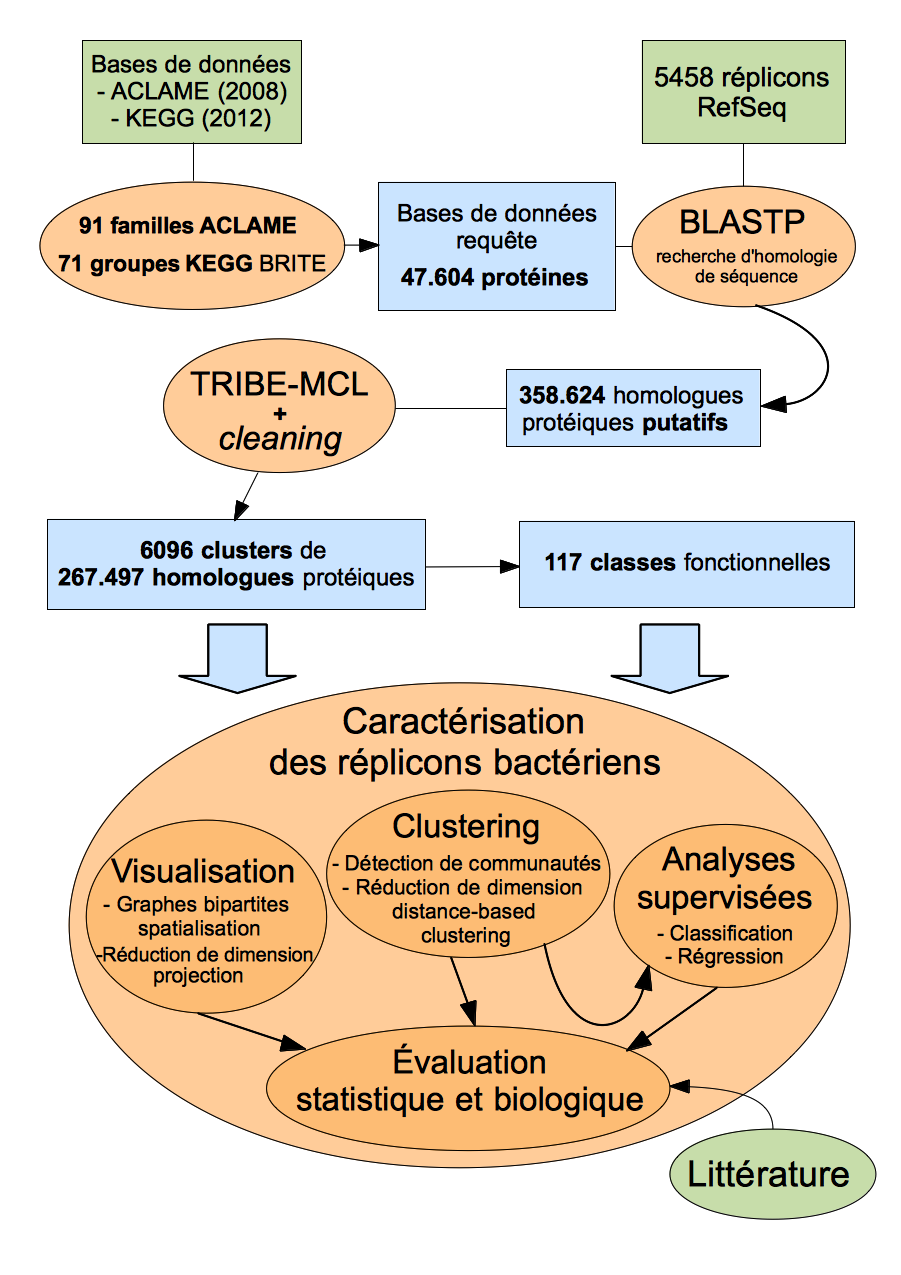
\includegraphics[width=\textwidth]{./img/workflow3.png}
\caption[Pipeline analytique]{Pipeline analytique.}
\end{center}
\end{figure}

\chapter{Construction de clusters de protéines homologues des STIG}\label{chap3b}
\lhead{\emph{Construction de clusters de protéines homologues des STIG}}

   
\section{Récupération des données brutes: les protéines des STIG des génomes}\label{pardonnebrut}
	La collecte des données représente la première étape du pipeline de l'analyse (Figure \ref{figstep1}). Deux sous-ensembles de données brutes peuvent être distingués: i) les séquences génomiques des réplicons et ii) les protéines des STIG.

\begin{figure}[H]
	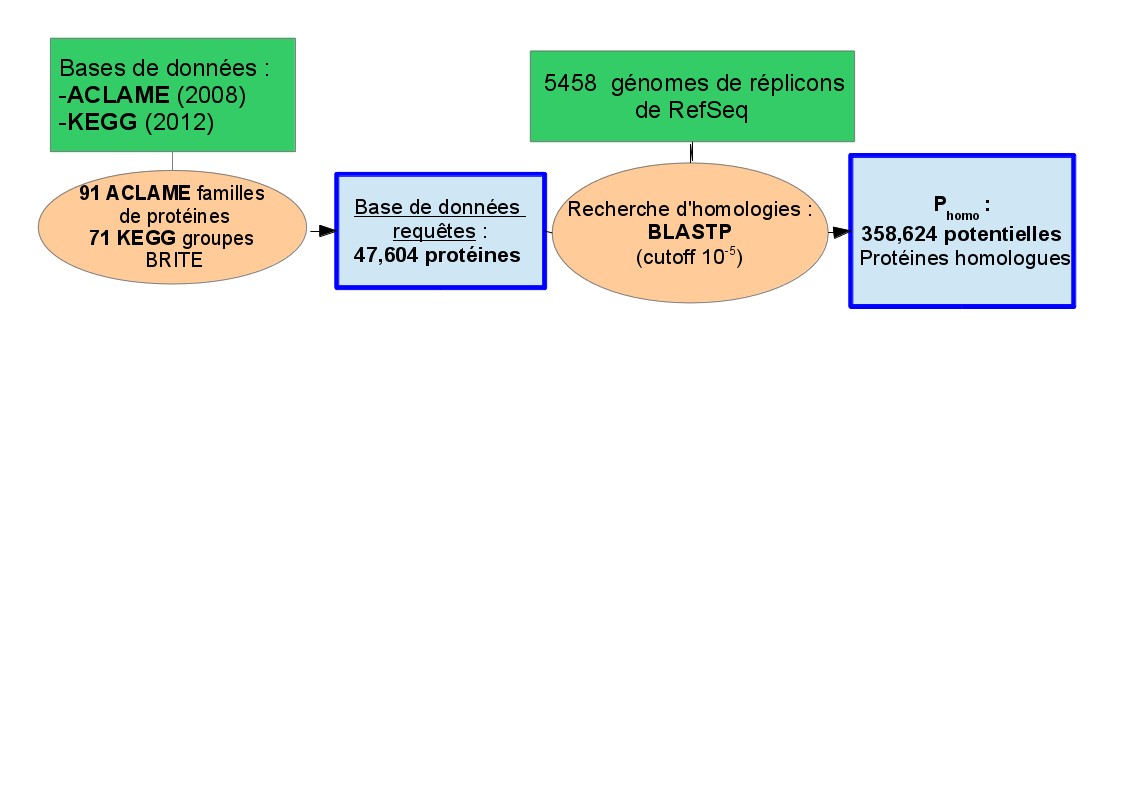
\includegraphics[width=\textwidth, trim= 0cm 12cm 0cm 0cm ,clip]{./img/workflow_sub1.png}
	\caption{Procédure de récupération des données brutes}\label{figstep1}
\end{figure}  

Obtenir une collection quasi-exhaustive des réplicons bactériens séquencés est une tâche aisée car ils sont accessibles dans les bases de données publiques majeures dont celles du NCBI. Par contre, nous avons à faire face à plusieurs difficultés pour la construction d'une base de données des protéines liées aux STIG:
\begin{itemize}
	\item Sélection d'un ou plusieurs système(s) d'annotation protéique parmi ceux proposés par les bases de données existantes.
	\item Sélection des annotations spécifiques aux STIG.
	\item Obtention des données les plus exhaustives possibles pour chaque fonctionnalité des STIG, pour chaque type de réplicon (plasmide et chromosome) et pour toute la diversité taxonomique bactérienne.
\end{itemize}

\subsection{Principales sources publiques de protéines annotées}
    \begin{description}
     \item[NCBI] (National Center for Biotechnology Information) rassemble des données de séquences d'acides nucléiques et de protéines accessibles \textit{via} internet. Les bases de données \textbf{RefSeq} \citep{pruitt2007ncbi} et \textbf{GenBank} \citep{benson2008genbank} sont gérées par le NCBI et constituent des collections de séquences (génomes, gènes, protéines...) parmi les plus importantes disponibles. Les protéines sont annotées partiellement selon leur fonction (vérifiées ou hypothétiques) mais aucun formalisme d'annotation n'est proposé. \textbf{Protein Clusters} regroupe différents clusters de protéines homologues annotées par fonction selon les catégories fonctionnelles des COG (clusters of orthologous groups) \citep{mcentyre2003clusters}, et \textbf{CDD}, rassemble des protéines ou alignements de protéines classés selon leurs motifs structurels \citep{marchler2007cdd}.
      \item[KEGG]  (Kyoto Encyclopedia of Genes and Genomes) est une base de données regroupant des données génomiques, chimiques et systémiques annotées au niveau fonctionnel \citep{Kanehisa2012}. En particulier, les données des génomes complètement séquencés sont hiérarchisées en fonction de leurs propriétés chimiques et systémiques (KEGG BRITE hierarchy), ce qui, concrètement, produit des groupes de protéines regroupées par annotations fonctionnelles.
	\item[ACLAME] (A CLAssification of Mobile genetic Elements) est une base de données dédiée aux données génomiques provenant des \textit{MGE} (Mobile Genetic Element, terme défini par ACLAME) rassemblant des données de phages, plasmides et transposons \citep{leplae2010aclame}. Des clusters de protéines sont accessibles et organisés par familles annotées par des termes de \textbf{G}ene \textbf{O}ntology (GO) \citep{gene2000gene} ou \textbf{PhiGO} (système propre d'ontologie).
	\item[PATRIC]  (PathoSystems Resource Integration Center) est un système d'information libre dont le but est de fournir un support à l'analyse des différents pathogènes bactériens \citep{wattam2014patric}. Elle comprend énormément de génomes bactériens de toutes les espèces, et rassemble les annotations de GO fournies par différentes méthodes d'annotations.
	\item[Pfam] est une large collection de familles de protéines qui sont représentées par des alignements de séquences multiples et des modèles de Markov, et selon leurs domaines fonctionnels \citep{finn2014pfam}.
	\item[TIGRFAM] est une base de données de familles de protéines similaire à Pfam \citep{haft2003tigrfams}.
	\item[PDB] (Protein Data Bank) est une base de données de protéines et séquences nucléotidiques comportant des informations structurales (structures 3D) \citep{rose2013rcsb}.
\end{description}


\subsection{Construction de la base de données requête}\label{donneerequete}
   
	Les bases de données KEGG et ACLAME ont été sélectionnées pour la constitution de la base requête de données protéiques. Leur avantage est de proposer des structures d'annotation plus rigoureuses que celles du NCBI. Les annotations proposées par Pfam et TIGRFAM quant à elles sont principalement liées à la fonction des domaines identifiés sur les protéines et permettent difficilement d'identifier de façon exhaustive des groupes de protéines clairement liées aux STIG.\\
	Le système de hiérarchie BRITE a été utilisé dans la base de données KEGG afin d'identifier \textbf{68} groupes d'orthologues affiliés aux différentes fonctions protéiques d’intérêt (Chapitre \ref{chap1a}). Ce système  permet d'organiser différents objets biologiques (notamment des familles de protéines) fonctionnellement (Figure \ref{figbrite}). Ces 68 groupes d'orthologues (Annexe \ref{AppendiceB}) réunissent un total de \textbf{43.757} protéines.

\begin{figure}[H]
	\hspace{-2cm}
	\begin{minipage}{\textwidth}
		\Tree[.BRITE [.Chromosome [.Prokaryote\_type [.Nucleoid\_associated\_proteins ] [.Partitioning\_proteins ]]] [.DNA\_Replication\_Proteins [.Prokaryote\_type  [.Initiation\_factor Initiation\_factor\_(bactéries) ] [.Termination\_Factors ]]] ]
			\end{minipage}
	\caption[Choix des termes KEGG BRITE]{Choix des termes KEGG BRITE pour la constitution de la base requête de données des protéines liées fonctionnellement aux STIG.}\label{figbrite}
\end{figure}

\textbf{91} familles ACLAME ont été selectionnées selon leurs annotations fonctionnelles (GO et PHI) (Table \ref{aclame}) et regroupent au total \textbf{3.847} protéines (Annexe \ref{AppendiceC}). Le choix des familles ACLAME a été effectué de façon semi-automatique. Différentes familles liées aux STIG ont d'abord été sélectionnées manuellement ce qui a permis d'identifier les annotations pertinentes. Les protéines potentiellement liées aux STIG ont alors été identifiées automatiquement parmi les 18.228 familles de protéines plasmidiques, puis confirmées manuellement.

\begin{table}[H]
\caption[Annotations utilisées pour la selection des Familles ACLAME]{Annotations utilisées pour la selection des Familles ACLAME \citep{leplae2010aclame}.}\label{aclame}
\begin{center}
\begin{tabular}{>{\bfseries\small}l >{\small}l}
{\normalsize Accession}&\textbf{\normalsize Description}\\
\hline
go:0003677 & DNA binding\\
575 & plasmid partitioning protein family ParB/Spo0J\\
go:0015616 & DNA translocase activity\\
576 & plasmid partitioning protein family ParM\\
go:0000146 & microfilament motor activity\\
go:0007059 & chromosome segregation\\
go:0015616 & DNA translocase activity\\
go:0007059 & chromosome segregation\\
go:0016887 & ATPase activity\\
go:0030541 & plasmid partitioning\\
go:0051302 & regulation of cell division\\
phi:0000196 & plasmid copy number control\\
\end{tabular}
\end{center}
\end{table} 
   
      L'ensemble des \textbf{47.604} ($43.757+3.847$) protéines de référence de  KEGG  et ACLAME est noté \textbf{$P_{ref}$}.  L'annotation d'une protéine $p \in P_{ref}$ selon sa famille de référence est désignée par $Ann(p)$. On distingue donc $Ann_{KEGG}(p)$ de $Ann_{ACLAME}(p)$. Les ensembles des familles d'orthologues de KEGG et des familles ACLAME sont notés $Cl_{KEGG}$ et $Cl_{ACLAME}$, respectivement. Enfin, pour tout $C_{i} \in Cl_{KEGG}$ et $C_{j} \in Cl_{ACLAME}$ on désigne par $Ann_{KEGG}(C_{i})$ et $Ann_{ACLAME}(C_{j})$ l'annotation d'une famille KEGG ou ACLAME donnée.
 

\subsection{Récupération des séquences protéiques à partir de RefSeq}
  L'ensemble des séquences complètes de réplicons disponibles a été récupéré le 23/11/2012 \textit{via} le site FTP de RefSeq. Les séquences protéiques (confirmées ou hypothétiques) codées par les gènes de \textbf{5.458} génomes ont été extraites pour un total de \textbf{6.903.452} protéines hypothétiques.
  

\subsection{Sources de biais possibles}\label{parsourcebiais}
	La combinaison des données de KEGG et ACLAME permet de regrouper des protéines annotées d'origines chromosomique et plasmidique. Différentes sources de biais sont possibles:
\begin{itemize}
	\item Certains groupes fonctionnels peuvent être trop spécifiques à un groupe d'espèces. C'est le cas notamment de Hda, DiaA, SeqA, EzrA, SlmA ou RacA qui sont spécifiques de la réplication de \textit{E. coli} et \textit{B. subtilis} notamment, et ne sont pas généralisables à des groupes distants de bactéries.
	\item A l'inverse, certaines familles protéiques (connues ou non) peuvent ne pas être représentées. C'est le cas par exemple de CtrA, Noc ou de YabA. Le choix de ne pas sélectionner ces protéines dépend du fait que celles-ci ne sont pas incluses dans les ensembles de protéines liées aux STIG identifiées précédemment. Ces protéines étant trop spécifiques de certains groupes bactériens, il n'a pas été développé de protocole exclusif d'extraction de leurs séquences. Cela risque de ne pas permettre la discrimination ou l'identification des tendances pour certains groupes de réplicons dont trop peu de leurs STIG seraient représentés dans les protéines sélectionnées.
	\item Il existe un biais d'échantillonnage des familles taxonomiques bactériennes parmi les génomes de réplicons  (Figure \ref{specieplot}). Ce biais peut donner trop de poids aux représentants des familles sur-représentées, et inversement pour les groupes très minoritaires. Il devra en être tenu compte.
	\item Enfin, d'éventuelles erreurs d'annotation des protéines peuvent fausser les résultats. Ce dernier biais, malheureusement, est difficilement estimable dans le cadre de notre étude.
  \end{itemize}
 

\subsection{Recherche d'homologues}\label{paralgoalign}
	Parmi les méthodes permettant d'évaluer l'homologie entre séquences protéiques ou nucléotidiques, on peut distinguer celles qui utilisent un alignement des séquences et celles dites “\textit{alignment-free sequence analysis}” qui répertorient le nombre de mots (ou \textit{k-mers}) communs entre deux séquences.\\
	Le calcul de distances évolutives entre séquences implique classiquement un alignement des séquences, les distances étant estimées à partir des taux de mutation ponctuelle ou des phénomènes d'insertion/délétion observables à partir de l'alignement. Dans certains cas, des phénomènes extrêmes (inversions, recombinaisons multiples) peuvent biaiser les résultats de ces méthodes, qui ne produiront pas d'alignement cohérent malgré l'existence d'homologie entre les séquences.\\
	Parmi les méthodes d'alignement de séquences (Table \ref{align}), on peut séparer celles qui effectuent un alignement global cherchant à aligner tous les résidus des séquences-requête, des méthodes d'alignement local où seulement des parties de séquences peuvent être alignées, ces dernières étant plus intéressantes dans le cas des séquences divergentes. On distingue les méthodes présentant des solutions algorithmiques \textbf{optimales}, des méthodes dites \textbf{heuristiques}, où les résultats sont plus ou moins approchés de l'optimum. On peut de plus distinguer les algorithmes permettant d'aligner des séquences deux à deux, de ceux qui produisent des alignements multiples. Enfin, certains algorithmes requièrent une base de données de séquences à laquelle sont comparées des séquences-requête et produisent des alignements significatifs par rapport à la base de données. 

\newpage
\begin{longtable}{@{\hspace{-2cm}}  >{\bfseries}p{0.18\textwidth} | >{\small}p{0.9\textwidth}}
	\caption[Principaux algorithmes d'alignement de séquences]{Principaux algorithmes d'alignement de séquences de séquences nucléotidiques ou protéiques}\label{align}\\
	 Needleman-Wunsch& (Algorithme de ) \citep{needleman1970general} Algorithme d'alignement global optimal servant à aligner les séquences deux à deux. \\[0.4cm]
	 Smith-Waterman & (Algorithme de ) \citep{smith1981identification} Algorithme d'alignement local optimal servant à aligner les séquences deux à deux. \\[0.4cm]
	BLAST & (\textbf{B}asic \textbf{L}ocal \textbf{A}lignment \textbf{S}earch \textbf{T}ool) \citep{altschul1990basic} Heuristique de recherche et d'alignement local de séquences, à travers une base de données. Différentes phases composent l'algorithme, les principales étant: la recherche de \textbf{\textit{k-mer}}, la construction d'un alignement local à partir des hits et l'évaluation de l'alignement (statistique de  Karlin-Altschul \citep{korf2003blast}). BLAST est une approximation de l'algorithme de Smith et Waterman, et est l'une des méthodes les plus utilisées dans la recherche d'homologie de séquences, le logiciel le plus utilisé étant la suite du NCBI \citep{Camacho2009}. Le programme PSI-BLAST \citep{altschul1997gapped} est une variante de BLAST, qui inclut des procédures itératives de l'algorithme initial afin d'augmenter sa sensibilité à l'identification d'homologues distants.\\[0.4cm]
	HMMER & \citep{finn2011hmmer} Suite de logiciels permettant l'analyse de séquences \textit{via} la création de Modèles de Markov Cachés (HMM pour \textit{Hidden Markov Model}) \citep{eddy1998profile}. À partir d'un alignement multiple de protéines de référence, l'algorithme construit un modèle ou \textit{profile} constitué d'une suite d'états possibles associés à des probabilités de réalisation afin de détecter et d'aligner des séquences homologues potentielles à partir d'une base de données de séquences de référence. \textit{hmmsearch}, algorithme inclus dans la suite HMMER, présente de meilleures performances (sensibilité et spécificité) que BLAST et PSI-BLAST dans la détection d'homologues \citep{Eddy2011}. \textit{Jackmmer}, un autre algorithme de la suite HMMER est une procédure itérative similaire à PSI-BLAST \citep{Eddy2013}.\\[0.4cm]
	 MUSCLE & \citep{edgar2004muscle} Actuellement un des algorithmes les plus performants et les plus populaires d'alignement multiple de séquences. La première étape de l'algorithme compare les séquences deux à deux par une distance de type \textit{k-mer} et produit un arbre de similarité entre les séquences. L'alignement des séquences est ensuite effectué en suivant les branches de cet arbre. Contrairement à BLAST, MUSCLE n'estime pas directement la probabilité qu'un alignement donné soit dû au hasard. 
	 \end{longtable}

	 Bien que produisant des solutions optimales, les algorithmes de Needleman-Wunsch et de Smith-Waterman présentent des complexités trop élevées pour être applicables à l'analyse de près de 7 millions de protéines avec presque 48.000 protéines-requête. Les procédures itératives, bien qu'intéressantes dans la recherche d'homologues éloignés (entre chromosomes et plasmides) présentent deux inconvénients: i) elles convergent moins rapidement, et ii) dans le cas de familles multigéniques (par exemple, les recombinases/intégrases), le feront difficilement et identifieront l'ensemble des protéines codées par la famille multigénique pour une protéine-requête proche de cette famille \citep{Guglielmini2013}. Les méthodes de type HMMER, bien qu'offrant de meilleures performances, dépendent grandement de la qualité des alignements de séquences fournis en entrée. La construction des alignements pour les différents groupes de protéines homologues identifiées constituerait une source supplémentaire de biais. Certains jeux de protéines (les protéines Xer notamment) produisent difficilement des alignements significatifs et une analyse de type HMMER reposant sur un alignement non-significatif constitueront un \textit{profile} source d'erreur \citep{wistrand2005improved}.\\
	\textbf{Le logiciel \textit{blastp} de la suite BLAST+ \citep{Camacho2009} a été choisi pour sa rapidité et sa fréquente utilisation dans la communauté pour le calcul de similarité de protéines.} Le seuil de rejet est fixé pour une $\mathbf{e_{value}}$ (probabilité d'obtenir un alignement significatif par hasard sachant la base de données et la protéine de référence) inférieure à $10^{-5}$. Les scores de BLAST sont calculés par rapport au nombre $r$ d'alignements locaux détectés (hits) de façon heuristique lors de la recherche de \textit{k-mers} \citep{korf2003blast}. Le calcul de la $e_{value}$ par BLAST peut être résumé par:
	\begin{equation}
		\begin{split}
			e_{value}&=-ln(1-p_{value})\\
			&\textrm{où:}\\
			p_{value}&=\frac{p_{value}'}{\beta^{r-1}(1-\beta)}\\
			&\textrm{avec:}\\
			p_{value}'&=\frac{e^{-S_{sum}}S_{sum}^{r-1}}{r!(r-1)!}  
		\end{split}
	\end{equation}
et où $\beta$ est une constante fixée. $S_{sum}$ est une fonction de la somme des scores $S_{i}$ des hits détectés significatifs et de différentes variables telles que la taille $T$ de l'espace de recherche selon l'algorithme utilisé \citep{korf2003blast}:
	\begin{equation}
		S_{sum}=K\sum_{i=1}^{r}S_{i}+f(r,T)
	\end{equation}
avec $K$ constante. Les $S_{i}$, scores des hits d'un alignement de deux séquences $s^{S_{i}}_{1}$ et $s^{S_{i}}_{2}$ de longueur $n$ peuvent être estimés par une équation de la forme  \citep{korf2003blast}:
	\begin{equation}
		S_{i}=\sum_{j=1}^{n} ln\left(\frac{Q_{s^{S_{i}}_{1},s^{S_{i}}_{2}}[j]}{P(s^{S_{i}}_{1}[j]).P(s^{S_{i}}_{2}[j])}\right)
	\end{equation}
où $P(s^{S_{i}}_{1}[j])$ et $P(s^{S_{i}}_{2}[j])$ sont les fréquences d’occurrences du $j$-ème caractère dans l'espace de recherche de  $s^{S_{i}}_{1}$ et de $s^{S_{i}}_{2}$ respectivement et  $Q_{s^{S_{i}}_{1},s^{S_{i}}_{2}}[j]$, la fréquence d'occurrences de la paire formée par le $j$-ème caractère de $s^{S_{i}}_{1}$ et de $s^{S_{i}}_{2}$ dans l'espace de recherche. \\
\\
	Certains travaux ont étudié le lien entre score et pertinence biologique des différents algorithmes de recherche de similarité de séquence \citep{Eddy2011}. En particulier, il a été mesuré qu'une $e_{value}$ inférieure à $10^{-3}$ entre deux protéines correspond à 99\% à des homologues fonctionnels (selon Pfam et leurs annotations de clan et pour une base de données de taille 192.987) \citep{Boekhorst2007}. Un \textbf{\textit{cutoff}} à $10^{-5}$ a été choisi et semble garantir un maximum de pertinence dans la recherche d'homologies fonctionnelles entre les protéines-requête et les protéines identifiées. Un des biais peut cependant provenir de protéines contenant des domaines fonctionnels multiples et pouvant présenter des $e_{value}$ très faibles avec des protéines partageant un de leurs domaines quoique possédant des fonctions totalement différentes \citep{Song2007}.\\ 
	\\
L'analyse des \textbf{6.903.452} protéines par les \textbf{47.604} protéines reliées aux STIG par \textit{blastp} en utilisant une $e_{value}$ seuil de $10^{-5}$ et les paramètres par défaut (\citep{Camacho2009} a identifié \textbf{358.624 protéines homologues}, dont l'ensemble est désigné \textbf{$P_{homo}$}. La $e_{value}$ d'une protéine $p$ par rapport à une protéine $q$ sera notée: $e_{value}(p,q)$.



\section{Réalisation de clusters d'homologues protéiques et fonctionnels}\label{parclusterhomo}
	Les protéines liées fonctionnellement aux STIG récupérées sont ensuite utilisées comme référence pour identifier des homologues fonctionnels dans les 5.125 réplicons de notre jeu de données. Ensuite, les protéines identifiées sont partitionnées selon leurs homologies de séquences \textit{via} une analyse de clustering \textbf{afin de créer des unités d'homologies structurales et fonctionnelles}. Enfin, une procédure de “nettoyage” est effectuée afin d'exclure les clusters les plus biaisés (Figure \ref{figstep2}). 
  
\begin{figure}[H]
	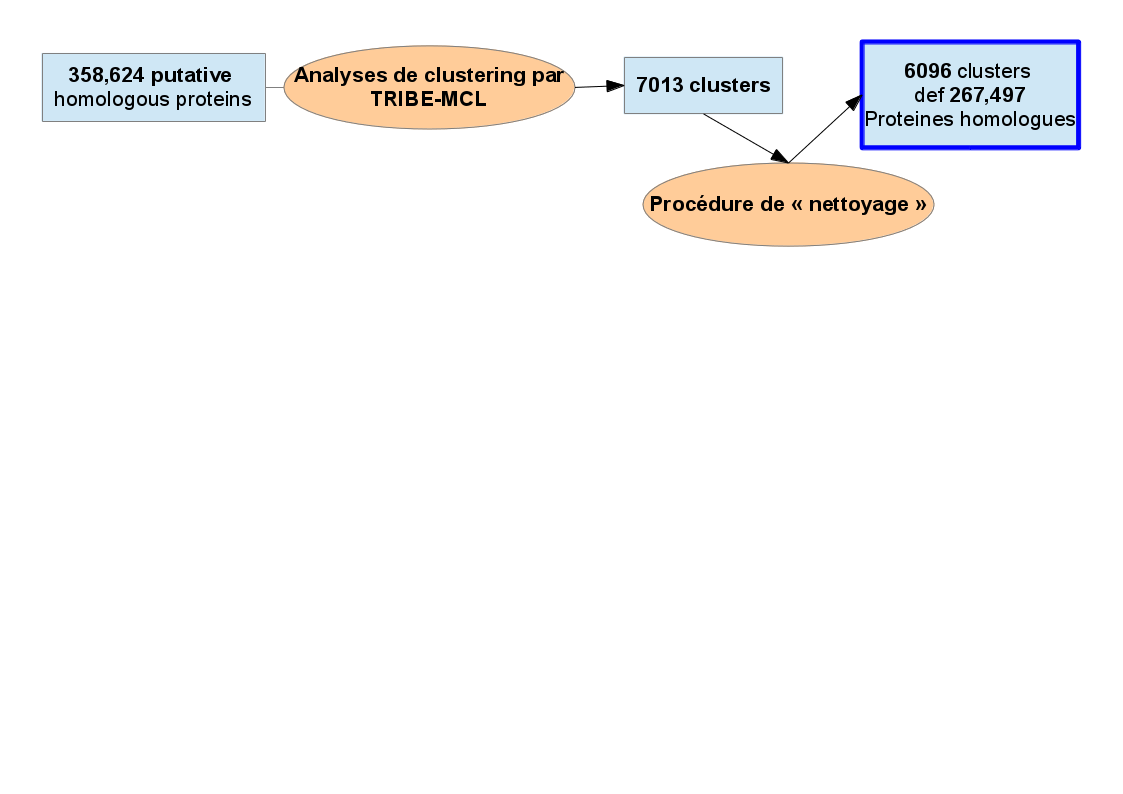
\includegraphics[width=\textwidth, trim= 0cm 14cm 0cm 0cm ,clip]{./img/workflow_sub2.png}
	\caption{Procédure de clustering des protéines}\label{figstep2}
\end{figure}  
	
Le choix et le paramétrage d'un algorithme de calcul d'homologie de séquences est suivi du choix et du paramétrage d'un algorithme de clustering de séquences protéiques. Différentes méthodes d'évaluation des clusters sont introduites. 



\subsection{Clustering des protéines}
\subsubsection{Définition}
	La majorité des algorithmes de clustering de séquences protéiques (ou nucléotidiques) reposent sur le calcul préalable d'une matrice de comparaison (aussi appelée matrice de distance ou de dissimilarité) de séquences deux à deux:
	\begin{description}
		\item[$\bullet$]  Pour un ensemble de $n$ protéines $P=\{p_{1},...,p_{n}\}$ et une distance $d$ calculant un degré de dissimilarité de séquence $d(p_{i},p_{j})$ entre deux protéines $p_{i}$ et $p_{j}$, soit $M^{d}$ la matrice de distance où: 
			\begin{equation}
				M_{ij}^{d}=d(p_{i},p_{j})
			\end{equation}
		\item[$\bullet$] $S^{d}$, la matrice de similarité, est alors définie par :
			\begin{equation}
				S^{d}_{ij}=1-\frac{d(p_{i},p_{j})}{d_{max}}
			\end{equation}
		\item[$\bullet$] Les graphes d'\textbf{I}nteraction \textbf{P}rotéines-\textbf{P}rotéines (\textbf{IPP}) sont des graphes où $S^{d}$ est la matrice d'adjacence du graphe $G=(P,E,S^{d})$, où $E$ est l'ensemble des couples $(p_{i},p_{j})$ pour lesquels une homologie significative a été detectée.
	\end{description}



\subsubsection{Principe}    
     Les algorithmes de calcul de similarité de séquences (Table \ref{align}) sont généralement utilisés pour le calcul de $e_{value}$ qui servent de distances inter-protéiques. La majorité des méthodes de clustering de protéines sont en fait des algorithmes de détection de communautés appliqués aux IPP \citep{Brohee2006,li2010computational}. Il existe de plus des critères externes spécifiquement développés pour les IPP. Un des biais potentiels dans l'utilisation des $e_{value}$ des algorithmes en tant que distances est qu'elles ne sont pas obligatoirement \textbf{métriques}. En effet, \textit{blastp} et \textit{phmmer}, par exemple, produisent des $e_{value}$ telles que $d(p_{i},p_{j}) \neq d(p_{j},p_{i})$\\
 
 
\subsubsection{TRIBE-MCL}
	L'algorithme de clustering \textbf{TRIBE-MCL} \citep{Enright2002} a été choisi pour son efficacité, démontrée notamment dans la construction des familles ACLAME \citep{leplae2010aclame}, pour sa capacité à regrouper des protéines multi-domaines \citep{Enright2002,Frech2010} et pour ses meilleures performances dans l'identification de familles protéiques \citep{Frech2010,apeltsin2011improving}. \\
	TRIBE-MCL est dérivé de l'algorithme Markov Cluster (MCL) \citep{van2000graph} qui est une méthode de détection de communautés. Le principe de l'algorithme est de capturer des clusters de protéines, régions du graphe où les protéines sont relativement plus interconnectées, en simulant des trajets aléatoires dans le graphe selon l'hypothèse qu'un trajet aléatoire dans un cluster tendra davantage à rester dans ce cluster que d'en sortir. Ces trajets aléatoires sont simulés \textit{via} des opérations sur la matrice d'adjacence du graphe par deux opérations matricielles: \textit{expansion} et \textit{inflation} \citep{Enright2002}. L'expansion a pour effet de dissiper les trajets aléatoires au sein des clusters, et l'inflation élimine les trajets inter-clusters. L'opération d'inflation est sous le contrôle d'un opérateur $gr$ qui, pour des valeurs élevées, augmente le “resserrement” (ou \textbf{granularité}) des clusters obtenus. Une valeur de $gr$ supérieure à 1 permet théoriquement la création de clusters. \\
TRIBE-MCL prend comme mesure de similarité entre deux protéines $p_{i}$ et $p_{j}$ :
	\begin{equation}
		d(p_{i},p_{j})=-log_{10}(e_{value}({p_{i},p_{j})})
	\end{equation}
	L'efficacité de TRIBE-MCL à reconstruire des familles protéiques dépend grandement de la granularité choisie et sera influencée par la nature des familles de protéines étudiées \citep{Frech2010,apeltsin2011improving}.  Ainsi, \textbf{la valeur optimale de $gr$ dépend du jeu de protéines analysé et de la question qu'on se pose.} 


\subsection{Identification des domaines fonctionnels des protéines}\label{pardomaine}
	Afin d'évaluer les clusters formés, les protéines ont été caractérisées selon leurs domaines fonctionnels. Pour l'identification des domaines des 358.624 homologues et des 47.604 protéines de référence, le programme \textit{hmmscan} de la suite HMMER a été utilisé avec la base de données Pfam du 03/03/2013 comme base de données de référence, et, comme valeurs seuils, $e_{value}<10^{-5}$ et  $ce_{value}<10^{-5}$ (\textit{conditionnal $ce_{value}$}). La $e_{value}$ pour un domaine est similaire à la $e_{value}$ précédemment définie. La $ce_{value}$ d'un domaine désigne la probabilité que le domaine ne soit pas significatif sachant que la protéine sur laquelle est trouvé le domaine est un vrai homologue d'une protéine de la base de données requête \citep{finn2011hmmer}. Les valeurs des autres paramètres sont celles par défaut \citep{Eddy2013}. L'ensemble des domaines identifiés dans un ensemble de protéines $P$ est noté $D_{P}$. De même, l'ensemble des domaines identifiés dans une protéine $p$ est noté $D_{\{p\}}$.  \textbf{1.175.018} et \textbf{127.853} profiles ont ainsi été identifiés sur les 358.624 protéines de $P_{homo}$ (ensemble des protéines homologues) et les 47.604 protéines de $P_{ref}$ (ensemble des protéines de référence), respectivement. \textbf{1711} profiles différents sont identifiés (Figure \ref{figdomain}), montrant l'hétérogénéité des protéines présentes.
	
\begin{figure}
	\begin{center}
	\begin{subfigure}{0.8\linewidth}
		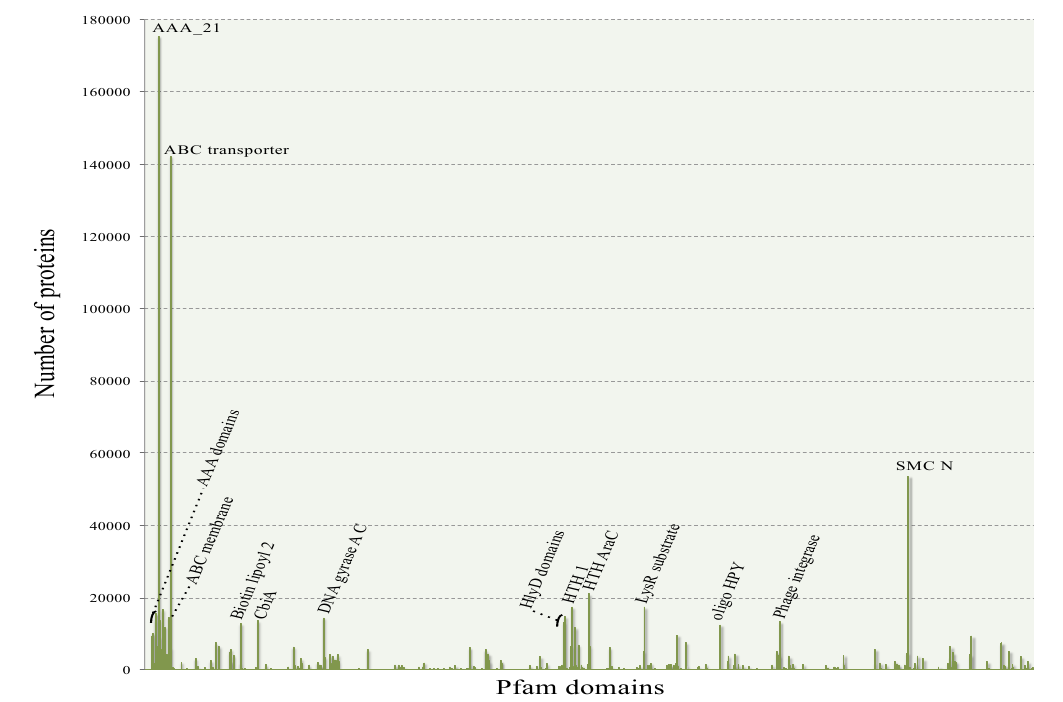
\includegraphics[width=\textwidth]{./img/domain_occurence.png}
		\caption{Distribution des domaines Pfam}\label{figdomain1}
	\end{subfigure}
	\\
	\begin{subfigure}{0.8\linewidth}
		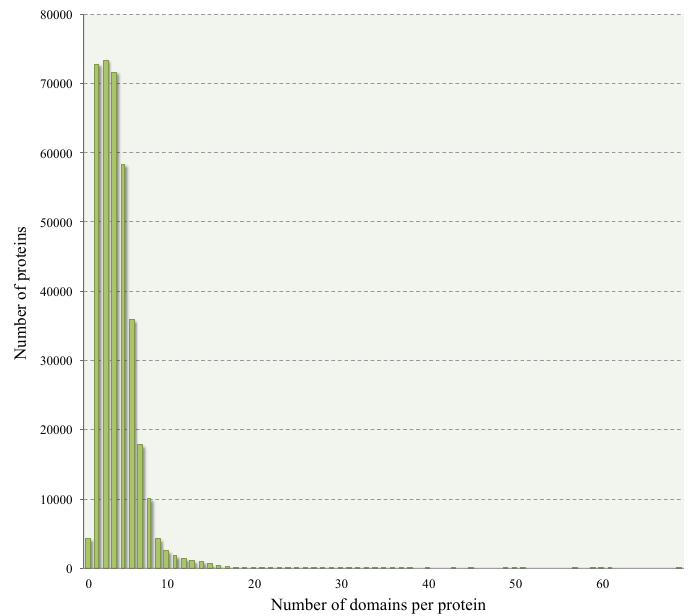
\includegraphics[width=\textwidth]{./img/domain_per_prot.png}
		\caption{Nombre de domaines par protéine}\label{figdomain2}
	\end{subfigure}
	\caption[Distribution des types et nombres d'occurence des profiles dans $P_{homo}$]{Distribution des types et nombres d'occurence des profiles dans $P_{homo}$. \ref{figdomain1}: Histogramme de l’occurrence des 1711 domaines Pfam identifiés. \ref{figdomain2}: Distribution des nombres de domaines Pfam par protéine.}
	\label{figdomain}
	\end{center}
\end{figure}



\subsection{Critères d'évaluation des clusters}
      L'évaluation des IPP se fait généralement sur des critères externes en les comparant à des familles ou classes de protéines de référence \citep{nepusz2012detecting}. 
\begin{description}
\item[$\blacktriangleright$] Il est possible d'utiliser des indices dérivés de la sensibilité/spécificité et du $F_{score}$ (éq. \ref{eqsensitive}) \citep{Brohee2006}.
\item[$\blacktriangleright$] D'autres chercheurs proposent d'évaluer la $p_{value}$ d'un cluster par rapport à une classe de référence selon leurs tailles \citep{li2010computational}. Pour un cluster $C$ contenant $k$ protéines appartenant à une classe de référence $F$, la probabilité que ce cluster ne soit pas formé par hasard selon $F$ est égale à:
      \begin{equation}\label{pvalue}
        p_{value}=1-\sum_{i=1}^{i=k-1}{\frac{ {|F| \choose i}{|P|-|F| \choose |C|-i} } {{|P| \choose |C|}}} 
      \end{equation}
\item[$\blacktriangleright$] Un autre indice important dans la selection de la granularité pour les IPP est l'\textit{intra-cluster clustering coefficient} (ICCC) \citep{Lima-Mendez2008,VanHoudt2012}. Soit une protéine $p$ de $P$, appartenant à un cluster $C$, et ayant un ensemble $N$ de protéines voisines incluses dans $C$, pour tout $i,j$ tels que $p_{i},p_{j} \in N$, le \textit{clustering coefficient} $CC_{p}$ de $p$ est défini par:
      \begin{equation}\label{ccv}
      	CC_{p}=\frac{\sum_{i=1}^{|N|-1}\sum_{j=i+1}^{|N|}S^{d}_{i,j} }{|N|.(|N|-1)/2}
      \end{equation}
L'ICCC est alors défini par : 
      \begin{equation}
      	ICCC = \sum_{p \in P}CC_{p}
      \end{equation}
\item[$\blacktriangleright$] Différents indices ont été utilisés pour répondre aux deux objectifs suivants: i) obtenir des clusters suffisamment homogènes en homologues fonctionnels et, ii) analyser les similitudes/dissimilitudes des réplicons \textit{via} les clusters obtenus. Deux types de références sont identifiables dans les jeux de données: i) les familles de protéines ACLAME et KEGG et leur annotations, et ii) les domaines Pfam identifiés.\\
 Pour tout $p \in P_{homo}$ et tout $p' \in P_{ref}$, une première annotation de $p$ est donnée par:
      \begin{equation}\label{eqannot}
      Ann(p)=Ann(p') \iff e_{value}(p,p')=min\{e_{value}(p,p'')| \: p'' \in P_{ref}\}
      \end{equation}
\begin{description}
 \item[\textbullet] L'objectif est d'estimer l'homogénéité en terme d'annotation des différents clusters mais l'\textbf{\textit{exhaustivité}} des clusters n'est pas recherchée. Pour cela un indice externe de comparaison dérivé du Biological Homogeneity Index (BHI) \citep{Datta2006} est alors calculé. Soit un clustering $Cl$ composé de $k$ clusters: $Cl=\{C_{1},...,C_{k}\}$. Le BHI est alors défini par:
	\begin{equation}
      	BHI=\frac{1}{|Cl|}\sum_{i=1}^{|Cl|}c_{i}
      \end{equation}
où $c_{i}$ est défini par:
      \begin{equation}\label{bhiwci}
      	c_{i}=\frac{2}{|C_{i}|.(|C_{i}|-1)}\sum_{p,q \in C_{i}}d(p,q)
      \end{equation}
sous l'hypothèse que, pour tout $p \in C_{i}, \; \exists \; Ann(p)$ où $d(p,q)$ est défini par:
      $$d(p,q) = 
      \begin{cases}
       1 & \text{si } Ann(p)=Ann(q)\\
       0 & \text{sinon }
      \end{cases}
      $$
Contrairement à l'indice initial, la constante “$2$” est ajoutée pour que le dénominateur soit de la forme $\frac{N.(N-1)}{2}$, qui est le nombre de paires dans $N$ éléments (on compare le nombre de \textit{cas} observés sur le nombre de \textit{cas} possibles, ainsi l'éq. \ref{bhiwci}, tout comme l'éq. \ref{ccmci} ci-après, est de la forme de l'éq. \ref{ccv}). En d'autres termes, le BHI est une mesure simple à interpréter, prenant ses valeurs dans $[0,1]$, qui est maximum si, pour tout cluster $C_{i}$ de $Cl$, toutes protéines $p$ de $C_{i}$ possèdent une même annotation: $Ann(p)$. Le BHI ne prend cependant pas en compte les potentielles grandes différences de taille entre clusters (ce qui est notre cas: Figure \ref{figclustersize}). Une correction du BHI est alors apportée pour donner le \textit{weighted BHI} (BHIw): 
	\begin{equation}\label{bhiw}
		BHIw=\frac{1}{|P|}\sum_{i=1}^{|Cl|}c_{i}.|C_{i}|
	\end{equation}
où $|P|$ est le nombre total de protéines du clustering (dans notre cas $|P_{homo}|$). 

\item[\textbullet] Avec pour objectif de mesurer l'\textit{\textbf{homogénéité}} des clusters, c'est-à-dire leur capacité à contenir des protéines ayant des domaines fonctionnels similaires, l'indice \textit{Conservation Consistency Measure} (CCM) est introduit. Le CCM est défini par:
	\begin{equation}\label{ccm}
		CCM =\frac{1}{|P|}\sum_{i=1}^{|Cl|}c'_{i}.|C_{i}|
	\end{equation}
où $c'_{i}$ est défini par:
	\begin{equation}\label{ccmci}
		c'_{i}=\frac{2}{|C_{i}|.(|C_{i}|-1)}\sum_{p,q \in C_{i}}d_{Jaccard}(D_{\{p\}},D_{\{q\}})
	\end{equation}
et où $d_{Jaccard}$ est la distance de Jaccard pour deux ensembles. L'indice CCM prend ses valeurs dans $[0,1]$. Une valeur proche de 0 indique des clusters qui contiennent des protéines ayant des domaines similaires.\\

\item[\textbullet] Enfin, on peut aussi calculer la proportion d'annotation majoritaire pour chaque cluster. Soient un cluster $C$, $Ann_{max}^{C}$ l'annotation majoritaire des protéines de $C$, et $N_{Ann_{max}^{C}}$ le nombre de fois que $Ann(p)=Ann_{max}^{C}$ pour tout $p \in C$. On définit $Pr_{ Ann_{max}}$ par:
	\begin{equation}\label{eqpourc}
		Pr_{ Ann_{max}}=\frac{N_{Ann_{max}^{C}}}{|C|}
	\end{equation}
\end{description}
\end{description}


      
\subsection{Génération de clusters aléatoires}\label{parclustaleat}
	L'évaluation des clusters formés ainsi que les procédures de “cleaning” (ci-après) font intervenir des clusters de protéines engendrés aléatoirement. Une protéine étant uniquement caractérisée par le nombre et le type de domaines qu'elle comporte, on peut distinguer trois processus aléatoires indépendants intervenant dans la génération aléatoire d'un cluster de protéines:
\begin{description}
	\item[$\bullet$] le nombre de protéines du cluster,
	\item[$\bullet$] le nombre de domaines fonctionnels présents dans une protéine donnée,
	\item[$\bullet$] le type d'un domaine donné.
\end{description}

\subsubsection{Variables}
Soit $X_{k}$, $X_{d}$ et $X_{t}$ les variables aléatoires discrètes et indépendantes correspondant aux nombre de protéines par cluster, nombre de domaines et type d'un domaine, respectivement. Les ensembles des valeurs possibles $E_{k}$, $E_{d}$ et $E_{t}$ sont alors déduits des données:
	\begin{description}
		\item[$\mathbf{E_{k}}$] prend ses valeurs entre $1$ (le nombre minimum de protéines dans un cluster) et $max\{|C|\;|\; C \in Cl\}$ pour un $Cl$ donné.
		\item[$\mathbf{E_{d}}$] prend ses valeurs entre $0$ (le nombre minimum de domaines fonctionnels identifiés dans une protéine donnée) et $max\{|D_{\{p\}}|\; p \in P_{homo}\}$.
		\item[$\mathbf{E_{t}}$] prend ses valeurs dans $D_{P_{homo}}$.
	\end{description}	    
De même, l'estimation des lois de probabilités de $P_{X_{k}}$, $P_{X_{d}}$ et $P_{X_{t}}$ se fait à partir des données:
	\begin{description}
		\item[$\mathbf{P_{X_{k}}}$] Soient $O_{Cl}=\{|C_{i}|, \;  C_{i} \in Cl\}$ la distribution des tailles des clusters d'un clustering, $Q^{q}_{O_{Cl}}=\{Q_{1},..,Q_{q}\}$ les q-quantiles de $O_{Cl}$, et $x_{(p/q)}$ la première valeur de $Q_{p}$ (avec $x_{((q+1)/q)}=+\infty$). On estime alors que:
			\begin{equation}\label{Xk}
				P_{X_{k}} \to
				\begin{dcases}
				P(x_{p/q}\leq X_{k}<x_{(p+1)/q})= \frac{|Q_{p}|}{|O_{Cl}|} & \textrm{ où } p \in \{1,...,q\}\\
				P(X_{k}=x_{p_{i}})=U([x_{p/q},x_{(p+1)/q}[)) &  \textrm{ où }  x_{p_{i}} \in [x_{p/q},x_{(p+1)/q}[\\
				\end{dcases}
			\end{equation}
		où $U$ est la loi uniforme discrète. D'une part la probabilité d'obtenir une valeur de taille $k$ incluse dans un certain intervalle dépend du nombre d'observations présentes dans cet intervalle et, d'autre part, toutes les valeurs de $k$ au sein d'un intervalle donné ont la même probabilité d'être tirées.
		\item[$\mathbf{P_{X_{d}}}$] En suivant la même démarche que pour $P_{X_{k}}$, on estime  que:
     			\begin{equation}\label{Xd}
				P_{X_{d}} \to
				\begin{dcases}
				P(x_{p/q} \leq X_{d}<x_{(p+1)/q})= \frac{|Q_{p}|}{|O_{P_{homo}}|} & \textrm{ où }   p \in \{1,...,q\}\\
				P(X_{k}=x_{p_{i}})=U([x_{p/q},x_{(p+1)/q}[)) &  \textrm{ où }  x_{p_{i}} \in [x_{p/q},x_{(p+1)/q}[\\      
				\end{dcases}
			\end{equation}
		avec  $O_{P_{homo}}$ la distribution du nombre de domaines par protéine des protéines de $P_{homo}$ et avec $Q_{p} \in Q^{q}_{O_{P_{homo}}}$.
		\item[$\mathbf{P_{X_{t}}}$] Soit $d$ un domaine de $D$. On note $N_{d}^{D}$ le nombre d'occurrences de $d$ dans $D$. $P_{X_{t}}$ est alors simplement estimé par: 
			\begin{equation}\label{Xt}
				P(X_{t}=d)=\frac{N_{d}^{D_{P_{homo}}}}{|D|}
			\end{equation}     
     \end{description}
La création d'un cluster aléatoire s'effectue par un premier tirage avec remise sur $X_{d}$ donnant la taille $x_{k}$ du cluster. On effectue alors $x_{k}$ tirages avec remise sur $X_{d}$ et, pour chaque valeur $x_{d}$ obtenue, on effectue finalement $x_{d}$ tirages avec remise sur $X_{t}$.   
    
\subsubsection{Loi de probabilité des clusters aléatoires}
	Les variables aléatoires $X_{k}$, $X_{d}$ et $X_{t}$ étant indépendantes, soient $X_{C}$ et $X_{Cl}$ les variables indépendantes discrètes correspondant aux tirages d'un cluster aléatoire et d'un clustering aléatoire, respectivement. Soient $C_{k,P}$, un cluster aléatoire constitué d'un ensemble de $k$ protéines $P=\{p_{1},...,p_{k}\}$, et $Cl_{rand}=\{C_{k_{1},P_{1}},...,C_{k_{z},P_{z}} \}$, un clustering aléatoire de $z$ clusters. On peut alors estimer que:
	\begin{equation}
		P(X_{C}=C_{k,P})=P(X_{k}=k).\prod_{p_{i} \in P}P(X_{d}=|D_{p_{i}}|).\prod_{d_{j} \in D_{p_{i}}}P(X_{t}=d_{j})
	\end{equation}
et que:
	\begin{equation}
		P(X_{Cl}=Cl_{rand})=\prod_{C_{k_{i},P_{i}} \in Cl_{rand}}P(X_{C}=C_{k_{i},P_{i}})
	\end{equation}

\subsubsection{Vérification par test d'hypothèses}
    Lorsqu'est calculé un clustering aléatoire $Cl_{rand}$ par rapport à un clustering observé $Cl$, une procédure de vérification est effectuée afin d'estimer si $O_{Cl_{rand}}$ et $O_{Cl}$, les distributions de taille des clusters de $Cl_{rand}$ et $Cl$, respectivement, suivent la même loi. Pour cela, un test d'indépendance du $\chi^{2}$ est réalisé entre $Q_{O_{Cl_{rand}}}^{p}$ et $Q_{O_{Cl}}^{p}$. Pour une $p_{value}$ du test supérieure à 0.05, on estime que les deux distributions ne sont pas statistiquement différentes.


\subsection{Protocole analytique}
    Pour chaque protéine de $P_{homo}$, une analyse \textit{blastp} est conduite sur $P_{homo}$ avec une valeur seuil de $e_{value}$ de $10^{-5}$ permettant l'obtention d'une matrice de similarité $S^{d}$, avec $d$ les $e_{value}$ données par \textit{blastp}. L'algorithme TRIBE-MCL est ensuite lancé sur $S^{d}$ en utilisant les granularités $gr$ suivantes: $(2,3,4,5,6,7,8)$, et les indices CCM, BHI et BHIw sont alors calculés pour les différents $gr$. La variance des scores des trois indices obtenus avec des clustering aléatoires (non représentée) est globalement très faible (de l'ordre de $10^{-5}$). La génération des clusters aléatoires a été réalisée en utilisant 1000 et 20 q-quantiles pour $O_{Cl}$ et $O_{D_{P_{homo}}}$, respectivement, avec $Cl$, les clusterings obtenus pour les différents $gr$. L'adéquation des distributions $O_{Cl}$ et $O_{Cl_{rand}}$ par le test du $\chi^{2}$ est estimée en utilisant 100 q-quantiles.
  
    
\subsubsection{Choix d'un $gr$ de travail}
	Les différents indices confirment l'efficacité de TRIBE-MCL pour la création de partitions pertinentes dans le cas de protéines homogènes en annotations et en contenu de domaines fonctionnels (Figure \ref{figclusteval}). 
	
\begin{figure}[H]
	\begin{center}
	\begin{tabular}{@{\hspace{-1.5cm}}cccc}
	\begin{turn}{90}\scriptsize\hspace{1.5cm} score BHI et BHIw \end{turn}&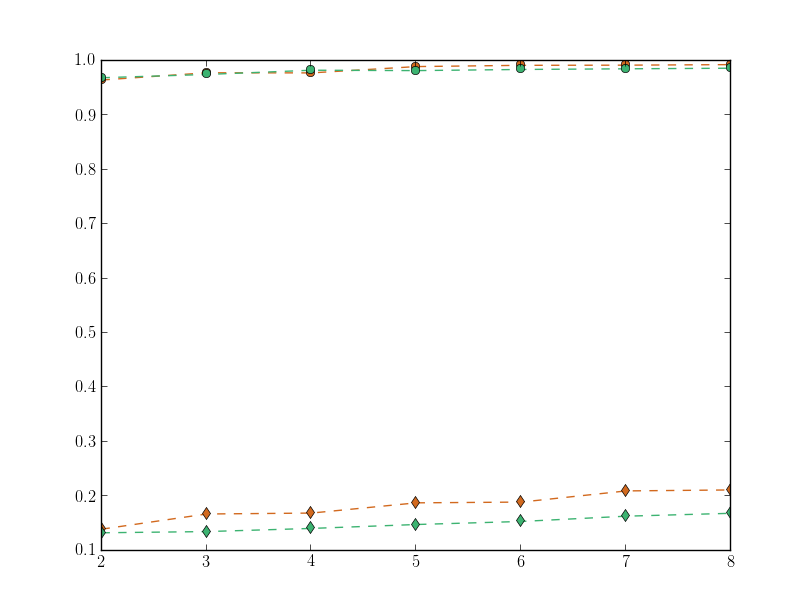
\includegraphics[width=0.50\textwidth, trim=15mm 10mm 9mm 0mm ,clip]{./img/clusteval1.png}&\begin{turn}{90}\scriptsize\hspace{1.5cm} score CCM \end{turn}&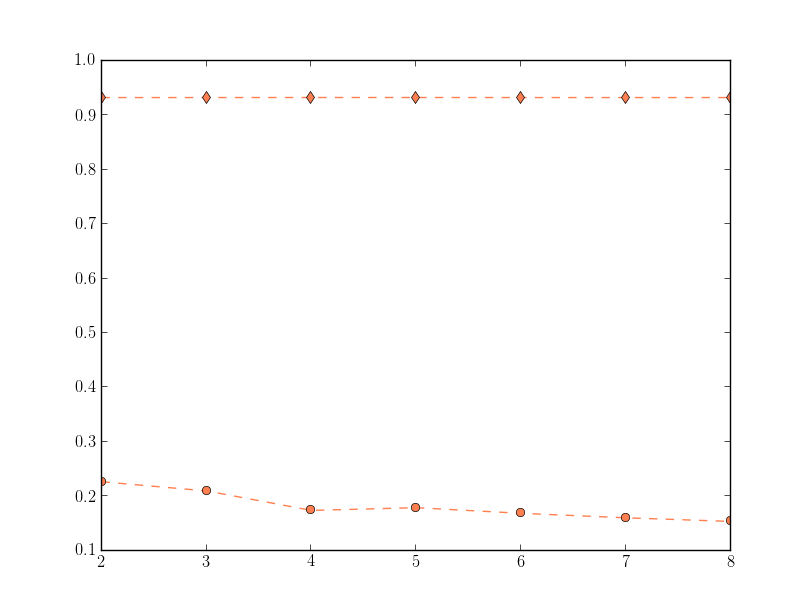
\includegraphics[width=0.50\textwidth, trim=15mm 10mm 9mm 0mm ,clip]{./img/clusteval2.png} \\
	&\scriptsize (A) Granularité&&\scriptsize (B) Granularité\\
	\end{tabular}
	\begin{tabular}{ccc}
	\begin{turn}{90}\scriptsize\color{blue}Nombre de clusters avec plus d'une protéines \end{turn}&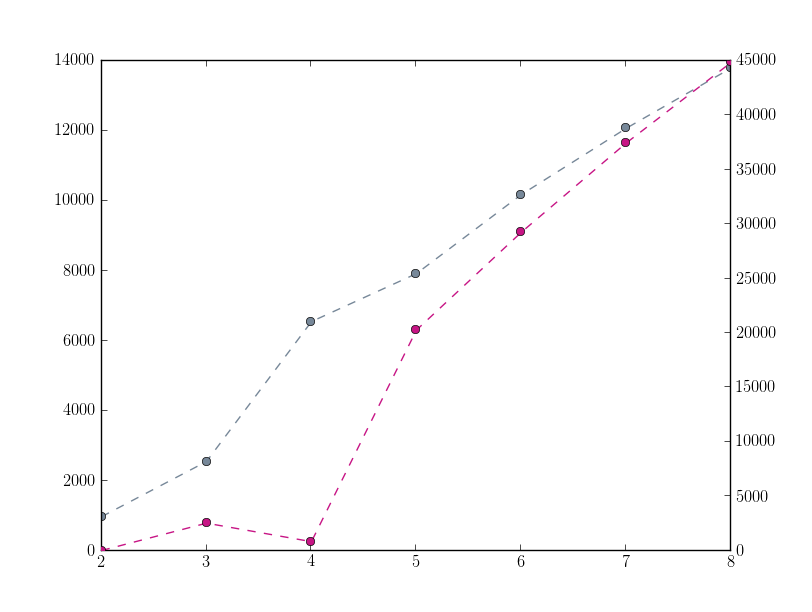
\includegraphics[width=0.50\textwidth, trim=15mm 10mm 9mm 0mm ,clip]{./img/clusteval3.png}&\begin{turn}{90}\scriptsize \color{magenta}\hspace{0.3cm}Nombre de clusters avec une protéine \end{turn}\\
	&\scriptsize (C) Granularité\\
	\end{tabular}
	\end{center}
	\caption[Influence de la granularité sur le clustering]{Influence de la granularité ($gr$) sur le clustering des protéines homologues des STIG. A: valeurs de BHI (orange), BHIw (vert). B: CCM (orange). C: Nombre de clusters de taille $>1$ (gris) et de taille $=1$ (rose). Losanges : résultats pour les clusterings engendrés aléatoirement.}\label{figclusteval}
	\end{figure}
    
Une augmentation de $gr$ semble accroître la performance de l'algorithme. Cependant, un $gr$ trop important ($gr\geq 3$) amplifie drastiquement le nombre total de clusters ainsi que le nombre de clusters ne contenant qu'une seule protéine. Une inflation trop importante semble ainsi avoir pour effet d'empêcher la détection de l'homologie entre protéines ou groupes de protéines, si elle est trop faible. Majorer $gr$ a donc pour effet de faire perdre de l'information entre protéines et entre réplicons, tout en renforçant la pertinence biologique des clusters (dans l'objectif d'avoir des clusters de protéines homologues au niveau fonctionnel). En imaginant des cas extrêmes, nous pouvons faire l'hypothèse qu'un $gr$ très important ne conservera l'homologie qu'entre des protéines très proches, appartenant vraisemblablement à des individus de la même espèce, et donc n'apportera pas d'information pertinente quant à la comparaison des différents réplicons. À l'inverse, un $gr$ trop faible aura pour tendance: i) de créer de fausses homologies entre certaines protéines et de produire des liens erronés entre réplicons, et ii) de créer des clusters de protéines non pertinents d'un point de vue biologique. \textbf{Un \textit{gr} de 4 apparaît ainsi être une valeur de travail pertinente}, pour laquelle les valeurs de CCM et BHIw sont améliorées (Figure \ref{figclusteval}).
\\
Un nombre raisonnable de clusters est produit tout en étant assez restrictif pour espérer séparer les groupes de protéines issues de familles multigéniques (Figure \ref{figclustersize}). La distribution en tailles $k$ des clusters (Figure \ref{figclustersize}) ne semble pas suivre de lois de probabilité classique.

\begin{figure}[H]
	\begin{center}
     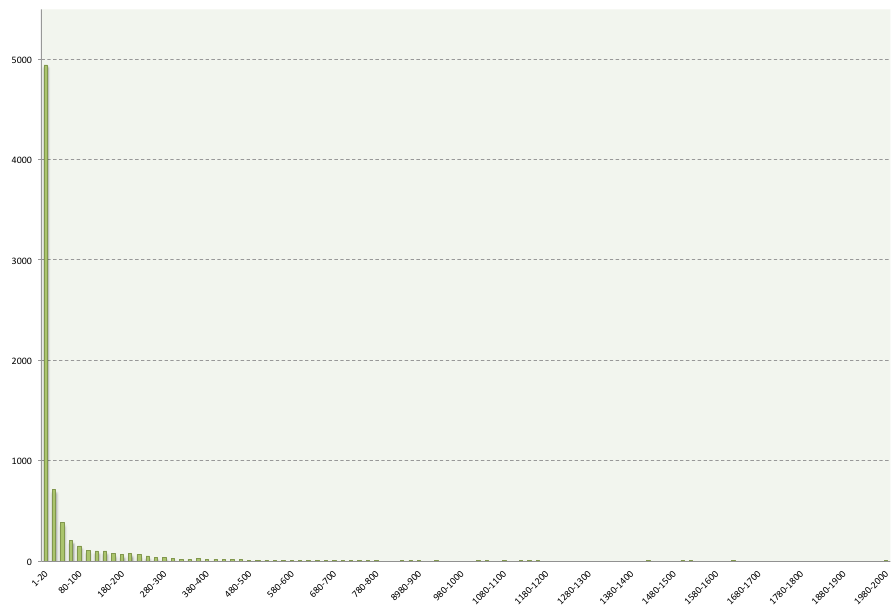
\includegraphics[width=0.8\textwidth]{./img/cluster_size.png}
    	\caption[Distribution de la taille des clusters de protéines pour $gr$ = 4]{Distribution de la taille des clusters de protéines pour un $gr$ de 4. \\ Abscisse : nombre de protéines par cluster. Ordonnée : nombre d'occurrence.}\label{figclustersize}
	\end{center}
\end{figure}
 
Malgré une très grande majorité de clusters homogènes obtenus pour un $Cl$ avec un $gr$ de 4 (Figure \ref{figannotdistib}), un faible pourcentage de clusters sont non-homogènes et regroupent des protéines ayant des annotations de fonctions proches (Table \ref{tabcausehetero}). Ce “bruit” semble être principalement lié à des familles multigéniques.
 \\

\begin{table}[H]
	\begin{center}
	\caption[Principales annotations multiples identifiées parmi les clusters]{Principales annotations multiples  identifiées parmi les clusters de protéines des STIG et pourcentage de ces annotations sur l'ensemble des clusters hétérogènes.}\label{tabcausehetero}
	\begin{tabular}{cc}
	\textbf{Annotations multiples} & \% \\
	\hline
	Ambiguïté XerC/XerD/Autres Xer & 38 \\
	Chromosomiques \textit{vs.} plasmidiques ParA & 11 \\
     Chromosomiques \textit{vs.} plasmidiques ParB & 6 \\
	Protéines DnaAB ambiguës & 5 \\
	Protéines Fts ambigües & 5 \\
     \end{tabular}
 \\ 
    
     \end{center}
\end{table}
     
\begin{figure}
      \begin{minipage}{0.5\textwidth}
      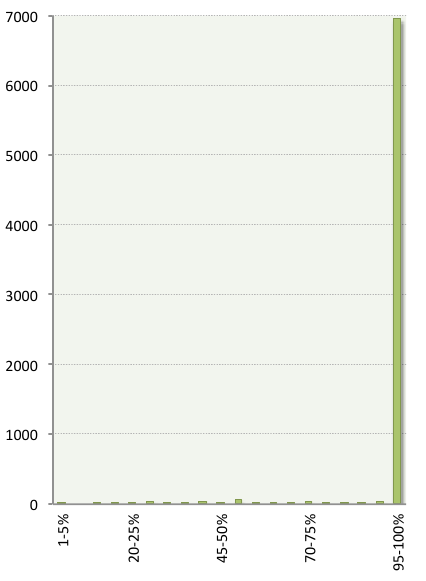
\includegraphics[width=\textwidth]{./img/protein_annot_distibA.png}
      \subcaption{}\label{figannotdistibA}
      \end{minipage}
      \begin{minipage}{0.5\textwidth}
      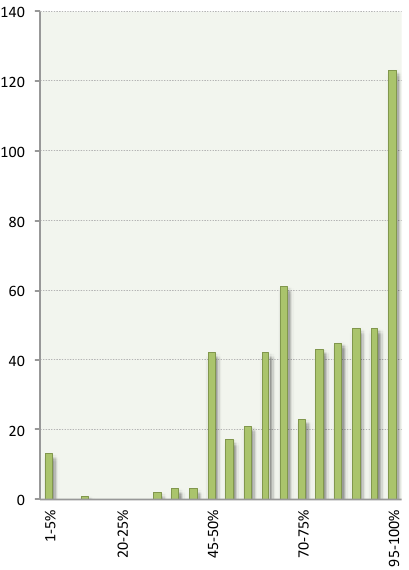
\includegraphics[width=\textwidth]{./img/protein_annot_distibB.png}            		\subcaption{}\label{figannotdistibB}
      \end{minipage}
      \caption[Pourcentage de l'annotation la plus fréquente par cluster]{Pourcentage de l'annotation la plus fréquente par cluster, parmi l'ensemble des clusters (\ref{figannotdistibA}) et parmi les clusters ayant des annotations multiples (\ref{figannotdistibB}). Les pourcentages sont calculés d'après l'éq. \ref{eqpourc}}\label{figannotdistib}.
\end{figure}    

\subsection{“Nettoyage” des clusters protéiques}\label{parcleaning}
	En raison de la présence de protéines avec des domaines fonctionnels multiples, un seuil de $10^{-5}$ pour l'analyse \textit{blastp} n'est pas suffisamment stringent pour garantir que la relation \ref{eqannot} est vérifiée dans tous les cas. Deux protéines partageant un même domaine fonctionnel peuvent être identifiées comme des homologues par une analyse de type \textit{blastp} bien que ne dérivant pas forcément d'une même protéine ancestrale \citep{Song2007}. Même si la question ici n'est pas de savoir si deux protéines ont une origine commune mais plutôt la même fonction, le problème reste identique: deux protéines peuvent posséder un domaine similaire (typiquement de type “transporteur ATP \textit{binding cassette}”, identifiant Pfam: ABC\_tran, par exemple) en addition d'un autre domaine, et cependant avoir des fonctions totalement différentes. Concrètement, on retrouve ce problème dans $P_{homo}$ avec, par exemple, l'obtention d'un cluster de protéines possèdant majoritairement un unique domaine de type “Sigma 54 modulation protein” (identifiant Pfam: Ribosomal\_S30AE). Ces protéines sont toutes liées à une protéine annotées XerC de \textit{Porphyromonas} (GI:332299940) qui comporte en plus d'un domaine de type intégrase, un domaine de type \textit{ABC\_tran}. Les protéines de ce cluster n'ont donc vraisemblablement pas le rôle d'intégrase et leur annotation XerC n'est donc pas pertinente.



\subsubsection{Procédure de nettoyage}
     Pour un cluster $C$, on définit son annotation $Ann(C)$ par:
	\begin{equation}
		Ann(C)=Ann(p) \iff N_{Ann(p)}^{C} = max\{N_{Ann(p_{i})}^{C}|\; p_{i} \in C \}
      \end{equation}
où $N_{Ann(p_{i})}^{C}$ désigne le nombre de fois que $Ann(p_{i})$ est trouvé pour les protéines de $C$.
Soit une protéine $p \in P$ avec $P=P_{ref} \cup P_{homo}$ et $D_{\{p\}}$ son ensemble de domaines fonctionnels. Le vecteur des domaines de $p$,  $v^{D_{P}}_{p}$, est alors introduit et est défini par: 
      \begin{equation}
		v^{D_{P}}_{p}=(N_{d_{1}}^{D_{\{p\}}},...,N_{d_{|D_{P}|}}^{D_{\{p\}}}),\;  d \in D_{P}
      \end{equation}
où $N_{d_{i}}^{D_{\{p\}}}$ est le nombre d'occurrences de $d_{i}$ dans $D_{\{p\}}$. Pour un cluster de protéines $C$, on peut définir son vecteur de domaines $v_{C}^{D_{P}}$ par:
      \begin{equation}
      	v_{C}^{D_{P}}=(\bar{N}_{d_{1}}^{C},...,\bar{N}_{d_{|D_{P}|}}^{C})
      \end{equation}
où $\bar{N}_{d_{i}}^{C}$ est défini par:
	\begin{equation}
       	\bar{N}_{d_{i}}^{C}=\frac{1}{|C|}\sum_{p \in C}N_{d_{i}}^{D_{\{p\}}}
	\end{equation}
Soit le clustering $Cl_{ref}$ formé des différentes groupes d'orthologues KEGG et familles ACLAME tel que $Cl_{ref}= Cl_{KEGG} \cup Cl_{ACLAME}$. Pour un clustering $Cl$ et pour tout $C_{i},C_{k} \in Cl$, on considère alors la distance:
      \begin{equation}\label{cleaningcosine}
      	d_{eval}(C_{i},C_{k})=d_{cosine}(v_{C_{i}}^{D_{P}},v_{C_{j}}^{D_{P}}) \textrm{ avec } \; C_{j} \in Cl_{ref} \textrm{ et } Ann(C_{k})=Ann(C_{j}) 
	\end{equation}       
avec $d_{cosine}$, la distance \textit{cosine}. Cette distance a une valeur unique pour chaque $C_{i}$ car il n'existe qu'un seul $C_{j} \in Cl_{ref}$ tel que $ Ann(C_{k})=Ann(C_{j})$. Soient un cluster $C_{i} \in Cl$ et un cluster aléatoire $C_{r}$ tels que $|C_{i}|=|C_{r}|$. Soit $X_{evalC_{i}}$, la variable aléatoire de $d_{eval}({C_{r},C_{i}})$ prenant ses valeurs dans $[0,+\infty[$. \textbf{On considère alors que $C_{i}$ est un cluster de $Cl$ valide si et seulement si:}
      \begin{equation}\label{eqseuil}
      	\begin{dcases}
      		d_{eval}(C_{r},C_{i})\leqslant x_{seuil_{i}}\\
      		P(x_{seuil_{i}} \leqslant X_{evalC_{i}})=0.90
      	\end{dcases}
      \end{equation}



\subsubsection{Estimation de $x_{seuil_{i}}$}
	Pour un cluster $C_{i} \in Cl$ donné, $n$ tirages avec remise de clusters aléatoires $C_{r_{i}}$ sont effectués avec $|C_{i}|=|C_{r_{i}}|$ en utilisant les estimations de $X_{d}$ et $X_{t}$ (relations \ref{Xd} et \ref{Xt}). Soient $Cl_{r_{i}}$ l'ensemble de ces clusters, $O_{Cr_{i}}=\{d_{eval}(C_{r_{i,1}},C_{i}),...,d_{eval}(C_{r_{i,n}},C_{i})\}$ l'ensemble des scores obtenus, et $Q_{O_{Cr_{i}}}^{10}$ ses déciles. On estime alors que:
     \begin{equation}
     x_{seuil_{i}}=x_{2/10}
	\end{equation}
	où  $x_{2/10}$ correspond à la première valeur du deuxième décile de $Q_{O_{Cr_{i}}}^{10}$.  



\subsubsection{Résultats et discussion}\label{parcleaningres}
	Cette procédure de cleaning consiste à évaluer si, pour un cluster de protéines $C$, les distributions en domaines fonctionnels de ses protéines se rapprochent de celles observées pour la famille de référence ayant la même annotation que $C$ ($Ann(C)=Ann(C_{ref})| \: C_{ref} \in Cl_{ref}$). On évalue avec l'éq.  \ref{cleaningcosine} la distance séparant les deux clusters. Les deux clusters ont des protéines ayant des domaines similaires si la distance observée est inférieure à 90\% des distances observées avec des clusters engendrés aléatoirement (éq. \ref{eqseuil}). \\
Le choix de la méthode de “cleaning”, ses performances, ainsi que de possibles méthodes alternatives sont discutés plus loin. Cependant, un des biais à souligner est celui lié à $D_{P_{homo}}$, qui intervient dans l'estimation de $X_{t}$ (éq. \ref{Xt}). À cause du jeu de protéines utilisé, certains domaines (tels que les domaines Pfam ABC\_tran ou Phage\_integrase) sont sur-représentés en comparaison à des domaines mineurs.  Ainsi, des clusters aléatoires formés avec des protéines comportant ces domaines seront plus probables et la méthode d'évaluation pour, par exemple, un petit cluster de recombinases sera plus restrictive. De plus, des protéines fausses positives $P_{FP}$ identifiées comme homologues à une protéine de référence multidomaines $p_{ref}$ peuvent avoir une partie de leurs domaines en commun avec $p_{ref}$ \citep{Song2007}, la procédure de cleaning ne prenant pas en compte ce biais dans la génération de clusters aléatoires. Enfin, un seuil de 10\% étant assez large, il en résulte que la procédure de cleaning est finalement peu restrictive et n'élimine que les clusters comportant des protéines présentant des distributions de domaines très biaisées par rapport à leurs familles de références $C_{ref}$ (Figure \ref{figannotclust}).\\ 
	En utilisant un $gr$ de 4, \textbf{917} clusters renfermant un total de \textbf{91.127} protéines, dont une large part est annotée “FtsE”, ont été identifiés comme n'étant pas valides (Figure \ref{figannotclust}A). Ces protéines sont vraisemblablement des membres de la superfamille des transporteurs ABC. Une partie importante des clusters valides est aussi annotée FtsE (Figure \ref{figannotclust}B). Ces protéines possèdent généralement un unique domaine ABC\_trans similairement aux “vraies” protéines FtsE. Il est alors probable que seules certaines d'entre elles ont une réelle fonction de type FtsE. On peut donc conclure que la seule utilisation de la distribution en domaines protéiques n'est pas toujours suffisamment discriminante pour l'identification des homologues fonctionnels. En considérant les seuils BLAST appliqués, on peut cependant supposer que ces protéines sont assez proches au niveau de leurs séquences et de leurs fonctions pour être tout de même maintenues dans notre jeu de données. 
	
\begin{figure}[H]
\begin{center}
\begin{subfigure}{0.7\textwidth}
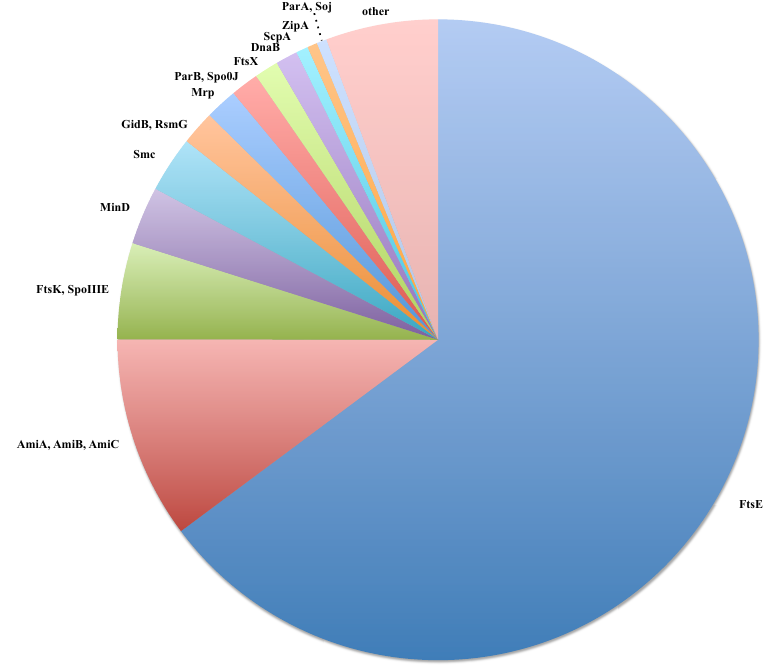
\includegraphics[width=\textwidth]{./img/cluster_noise.png}
\caption{Annotations des 917 clusters considérés comme \textit{incorrects}}
\end{subfigure}
\\
\vspace*{1cm}
\hspace{1cm}
\begin{subfigure}{0.8\textwidth}
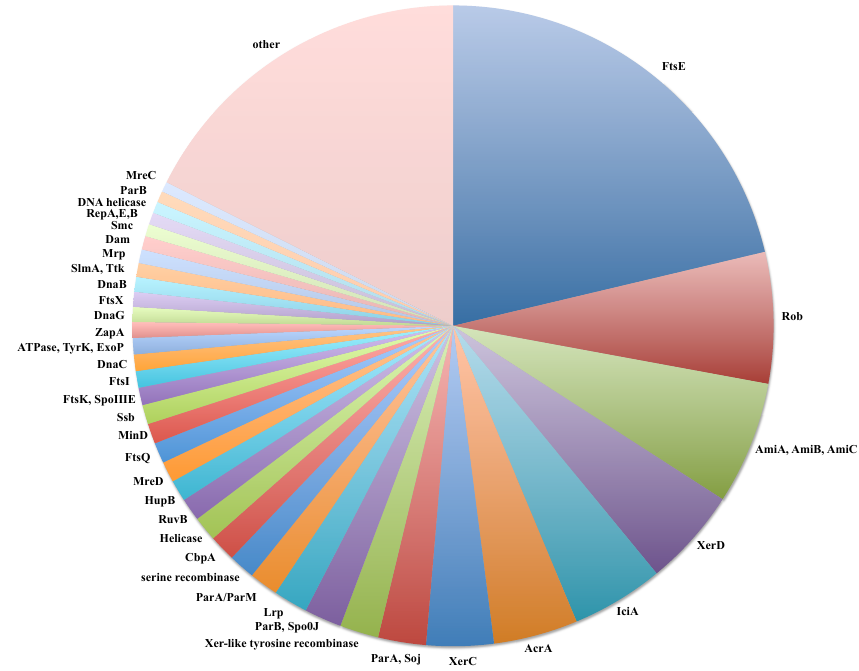
\includegraphics[width=\textwidth]{./img/cluster_annotate.png}
\caption{Annotations des 6465 clusters pertinents}
\end{subfigure}
\caption[Annotation des clusters de protéines]{Annotations des clusters de protéines. \\ Les clusters sont annotés selon l'annotation majoritaire des protéines qu'ils renferment (éq. \ref{eqannot}).}\label{figannotclust}
\end{center}
\end{figure}


\subsubsection{Alternatives à la procédure de cleaning} 
	D'un point de vue méthodologique, la procédure de cleaning utilisée est similaire à une procédure de classification supervisée, effectuée pour chaque cluster de protéines obtenu $C$ avec comme training set $E_{training}=\{E_{True},E_{False}\}$. D'une part, l'ensemble $C_{ref}$ des protéines a la même annotation que $C$ ($E_{True}$) et, d'autre part, des clusters de protéines engendrés aléatoirement $C_{r}$ selon la taille de $C$ correspondent à la distribution du type et du nombre de domaines de l'ensemble des protéines récupérées par l'analyse par \textit{blastp} ($E_{False}$). Différentes alternatives au calcul de la distance de l'éq. \ref{eqseuil} peuvent alors être envisagées:
\begin{description}
	\item[$\bullet$] Utiliser des algorithmes de classification supervisée classiques avec $E_{training}=\{C_{ref},C_{r}\}$. Les protéines, en fonction de leurs domaines, sont alors classées comme étant similaires à $C_{ref}$ ou à $C_{r}$ et, en fonction du nombre de protéines identifiées positives, $C$ est accepté ou refusé. Un des problèmes sous-jacents est de choisir les éventuels paramètres des algorithmes.
	\item[$\bullet$] Trier directement les protéines (et non les clusters) \underline{avant} d'effectuer la procédure de clustering par TRIBE-MCL. Un des inconvénients de cette approche est la possibilité d'éliminer des protéines $TP$ regroupées dans des clusters $TP$ grâce à leur homologie de séquence et étant de vrais positifs bien que n'ayant pas de domaines fonctionnels identifiés. Cela est toutefois peu probable, /\textit{hmmscan} étant beacoup plus sensible que /\textit{blastp}.
	\item[$\bullet$] Modifier $E_{training}$ en incluant, par exemple, un ensemble plus large de protéines témoins $TN$ dans $E_{False}$. Afin de compenser les biais introduits par des clusters $FP$ identifiés par l'analyse à cause de la présence d'un domaine commun avec certaines protéines $TP$,  $E_{False}$ pourrait être constitué de clusters de protéines aléatoires ayant la même annotation que les protéines de $E_{True}$. Il est cependant possible que cette procédure rende l'étape de cleaning beaucoup trop discriminative, en particulier pour les petits clusters. Il aurait été également intéressant de tester $C$ contre l'ensemble des $E_{True}$, et pas seulement contre l'ensemble présentant la même annotation que $C$, afin de  limiter les ambiguïtés pour les annotations proches comme XerC/XerD. 
	\item[$\bullet$] Inclure des données protéiques supplémentaires comme, par exemple, la taille et la synténie des domaines ou les données issues d'autres bases de données (TIGRFAM...).
	\item[$\bullet$] Utiliser une méthode tirée de la littérature pour la discrimination fonctionnelle des protéines par leurs domaines. Song \textit{et. al} \citep{song2008sequence} proposent une méthode similaire reposant sur une classification par régression logistique et des pondérations différentes des domaines et des séquences. Cependant, des problèmes similaires dans la classification de protéines ayant des domaines fréquents (exemple pKinase) sont mis en avant. Enfin, différentes alternatives à MCL peuvent être prometteuses dans l'identification d'homologues \citep{Terrapon2014}.
\end{description}

Trouver la procédure optimisant le nombre de protéine $TP$ présentes, homologues aux protéines de $P_{homo}$, et limitant le nombre de protéines $FP$ demande des études additionnelles qui n'ont pas été la priorité de cette étude. La difficulté, ici, est que les protéines de $P_{homo}$ appartiennent à différentes familles et présentent différents types d'homologies (Figure \ref{figtyrrec}). Ainsi, un cluster peut être constitué de l'aggrégation de différents sous-ensembles de protéines homologues et, inversement, différents clusters peuvent appartenir à un même niveau d'homologie. La structuration des clusters est de plus fortement influencée par le choix des paramètres, ici, $gr$ pour TRIBE-MCL, et dépend aussi des familles de protéines considérées.

\begin{figure}[H]
\Tree[.{tyrosine-recombinase} [ .Xer XerC XerD XerH ] [ .{tyrosine-intégrase} {phage-intégrase} {plasmide-intégrase} ] ]
\caption{Différents niveaux d'homologie chez les tyrosine-recombinases}\label{figtyrrec}
\end{figure}

\newpage
\chapter{Séparation des réplicons}\label{chap4b}

\lhead{\emph{Séparation des réplicons}}\label{parclassifrepl}

Les clusters de protéines obtenus sont ensuite utilisés pour caractériser les réplicons bactériens. L'objectif est de séparer les réplicons sur cette base et de voir si des regroupements spécifiques émergent. Les réplicons sont d'abord visualisés par des techniques de projection ou après transformation en graphe. Ensuite, ils sont clusterisés afin d'explorer plus spécifiquement les groupes formés et le positionnement des RECE par rapport aux autres réplicons.

\section{Jeux de données obtenues et notations}\label{parjeuxdedonnees}
    
\subsection{Classification taxonomique}

Les génomes bactériens sont organisés  selon leur classification taxonomique, la hiérarchie des différents rangs taxonomiques suivant la relation:
	\begin{equation}\label{eqtax}
	\text{Espèce} \subset \text{Genre} \subset \text{Famille} \subset \text{Ordre} \subset{Classe} \subset {Phylum} \subset \text{Domaine}
	\end{equation}
Un individu (souche) d'une espèce bactérienne est caractérisé par son génome $g$, constitué d’un ou plusieurs réplicons. Soit $G=\{g_{1},...,g_{|G|}\}$, l'ensemble des génomes bactériens. On peut définir un génome $g$ donné par l'ensemble des réplicons de différents types $r_{i}$ qui le constituent:
	\begin{equation}\label{eqindiv}
	g= \{r_{1},...,r_{|g|}\}
	\end{equation} 

\subsection{Description des réplicons}

On attribue aux réplicons le descripteur taxonomique de la bactérie qui les héberge. Ils possèdent de plus un type appartenant à l'ensemble $\{ \text{chromosome, plasmide, RECE} \} $ (``\textbf{chr}" est utilisé comme notation abrégée de “chromosome” dans les équations).
Les clusters d’homologues de protéines des STIG permettent de caractériser les réplicons. Soient une solution de clustering des protéines $Cl=\{C_{1},...,C_{|Cl|}\}$, et l'ensemble des réplicons $R=\{r_{1},...,r_{|R|}\}$. Un réplicon $r$ peut être décrit par l'ensemble des gènes codant des protéines qu'il porte et est  \textit{de facto} défini par un ensemble de protéines:
	\begin{equation}
	r=\{p_{1},...,p_{n}\}
	 \end{equation}
 Un clustering de $R$, tel que $f_{clustering}(R)=\Big\{\{r_{k_{1}1},...,r_{k_{1}i}\},...,\{r_{k_{x}1},...,r_{k_{x}j}\}\Big\}$, est noté $Kl$.\\
 Un réplicon $r$ est caractérisé par le vecteur $v^{r}$ défini par:
  	\begin{equation}\label{eqvr}
  	v^{r}=(N^{r}_{C_{1}},...,N^{r}_{C_{|Cl|}})
	\end{equation}
	où  $N^{r}_{C_{i}}=|r \cap C_{i}|$ est le nombre de protéines de $r$ dans $C_{i}$, un cluster de protéines homologues.\\	
L'ensemble $V^{R}$ des vecteurs $v^{r}$ pour les réplicons $r$ de $R$  alors défini par:
	\begin{equation}\label{eqV}
	V^{R}=\{v^{r_{1}},...,v^{r_{|R|}}\}
        \end{equation}		

\subsection{Groupes structuraux et taxonomiques}

Soit une classe $K$ de réplicons. On  définit le vecteur pondéré des réplicons de $K$ par:
	\begin{equation}
	\bar{v}^{K}=(\bar{N}^{K}_{C_{1}},...,\bar{N}^{K}_{C_{|Cl|}})
	\end{equation}
où $\bar{N}^{K}_{C_{i}}$ est défini par:
	\begin{equation}
	\bar{N}^{K}_{C_{i}}=\frac{1}{|K|}\sum_{r \in K}N^{r}_{C_{i}}
	\end{equation}
$\bar{v}^{K}$ est alors le centre de gravité de la classe $K$.\\
Les réplicons étant organisés par type et par groupe taxonomique, les notations suivantes sont introduites:
\begin{description} 
\item[$\bullet$] $R_{taxon}$ désigne l'ensemble des réplicons de $R$ dont l'hôte appartient au groupe taxonomique $taxon$. $V^{R_{taxon}}$ désigne, par extension, l'ensemble des vecteurs $v^{r}$ des réplicons $r$ de $R_{taxon}$. 
\item[$\bullet$] $R^{\{type\}}$ désigne l'ensemble des réplicons, $r \in R$, où $Type(r) \in \{type\}$ et où $Type(r)$ est la fonction renvoyant le type de $r$.
\item[$\bullet$]  Pour un réplicon $r$ donné, la fonction $Tax_{n\_tax}(r)$ renvoie la valeur du rang taxonomique considéré de $r$ avec \textit{n\_tax} appartenant à la relation \ref{eqtax}. Par exemple, $Tax_{phylum}(r)=\text{\textit{Protéobactéries}}$ ou $Tax_{class}(r)=\text{\textit{Beta-protéobactéries}}$.
\item[$\bullet$] $Kl_{n\_tax}^{R}=\{K_{1},...,K_{|Kl|}\}$ est  l'ensemble des classes $K_{i}$ de réplicons où $K_{i} \subset  R$  tel que:
	 $$\begin{dcases}
	   Tax_{n\_tax}(r_{x})=Tax_{n\_tax}(r_{y}) &  r_{x},r_{y} \in K_{i}\\
	   Tax_{n\_tax}(r_{x})\neq Tax_{n\_tax}(r_{z}) &  r_{z} \in K_{j,\; j\neq i}\\
	  \end{dcases}
	   $$ 
Par exemple, $Kl_{phylum}^{R}$ sera l'ensemble des réplicons de $R$ organisés en classes selon le phylum d'appartenance de leur hôte.
\end{description}
	    
L'ensemble $\bar{V}^{Kl_{n\_tax}^{R}}$ des $\bar{v}^{K_{i}}$  où $K_{i} \in Kl_{n\_tax}^{R}$ est alors défini par:
	    \begin{equation}
	    \bar{V}^{Kl_{n\_tax}^{R}}=\{\bar{v}^{K_{1}},...,\bar{v}^{K_{|Kl_{n\_tax}^{R}|}} \}
	    \end{equation}
On définit $\bar{V}^{R}_{n\_tax}$ comme l'ensemble des vecteurs de réplicons de $R$ normés selon \textit{n\_tax} et regroupés par $type$ tel que:
	     \begin{equation}\label{eqVnorm}
	     \bar{V}^{R}_{n\_tax}= \bar{V}^{Kl_{n\_tax}^{R^{ \{chr\} }}} \cup \bar{V}^{Kl_{n\_tax}^{R^{ \{plasmide\} }}} \cup \bar{V}^{Kl_{n\_tax}^{R^{ \{RECE\} }}}
	     \end{equation}
Par extension $\bar{V}^{R_{taxon}}_{n\_tax}$ désigne l'ensemble des vecteurs de réplicons de $R_{taxon}$ normés selon $n\_tax$ et regroupés par type.\\

Pour un ensemble $Kl_{n\_tax}^{R_{i}}$ donné avec $R_{i} \subset R$, et pour $K \in Kl_{n\_tax}^{R_{i}} $, si tous les réplicons de $K$ sont du même type, on peut annoter $K$ selon les valeurs de $Tax_{n\_tax}(r)$ et de $Type(r)$ où $r \in K$. De même que pour un réplicon, on peut alors définir $Tax_{n\_tax}(K)$ et $Type(K)$ tels que $Tax_{n\_tax}(K)=Tax_{n\_tax}(r)$ et $Type(K)=Type(r)$ pour $r \in K$. On définit $\bar{Kl}_{n\_tax}^{R_{i}}$, l'ensemble des couples (\textit{Type}, $Tax_{n\_tax}$) existant dans $R_{i}$ par:
	\begin{equation}
	\bar{Kl}_{n\_tax}^{R_{i}} =\Big\{ \{Type(K) , Tax_{n\_tax}(K)\} |\;K \in  Kl_{n\_tax}^{R_{i}}\Big\}
	\end{equation}
$\bar{Kl}_{n\_tax}$, l'ensemble des couples (\textit{Type}, $Tax_{n\_tax}$) existant dans R est alors défini par:
	\begin{equation}
	\bar{Kl}_{n\_tax}=\bar{Kl}_{n\_tax}^{R^{ \{chr\} }} \cup \bar{Kl}_{n\_tax}^{R^{ \{plasmide\} }} \cup \bar{Kl}_{n\_tax}^{R^{ \{RECE\} }} 
	\end{equation}
	
  \subsection{Dimension des données}    
Sur l'ensemble des 5125 réplicons considérés et sur les \textbf{267.497} homologues identifiés (358.624 homologues présumés diminués des 91.127 faux positifs) pour une granularité $gr$ de 4 pour TRIBE-MCL, \textbf{4928} réplicons codent au moins une protéine parmi les homologues. \textbf{6096} clusters de protéines sont formés et sont considérés comme authentiques (ils ne correspondent pas à de faux positifs).

\begin{table}[H]
 	\caption[Dimension des données utilisées]{Dimension des données utilisées.\\ $R$ est l'ensemble des réplicons ayant au moins une protéine homologue. $Cl$ est la solution de clustering obtenue pour un $gr$ de 4 après la procédure de \textit{cleaning}.} 
	\begin{center}
 	\begin{tabular}{c|c|c}
 	\textbf{Données} & \textbf{Matrice} & \textbf{Taille}\\
	\hline
	$R$ & - & 4928\\
	$Cl$ & - & 6096\\
	$V^{R}$ & $M^{V^{R}}$ & (4928,6096)\\
	$\bar{V}^{R}_{genre}$ & $M^{\bar{V}^{R}_{genre}}$ & (851,6096)\\
	$\bar{V}^{R}_{classe}$ & $M^{\bar{V}^{R}_{classe}}$ & (91,6096)\\
	$\bar{V}^{R}_{phylum}$ & $M^{\bar{V}^{R}_{phylum}}$ & (60,6096)\\
	\end{tabular}
	\end{center}
\end{table}
    
    
\section{Méthodes d'évaluation de la séparation des réplicons}
    
    L'évaluation des méthodes de clustering est fondée sur des critères internes et/ou externes. Dans le cas de critères externes, la difficulté est de choisir les classes de référence auxquelles les clusters obtenus seront comparés. Ici, les clusters de réplicons obtenus sont analysés des points de vue structural (selon le type de réplicons) et taxonomique. L'efficacité des différentes méthodes de visualisation des données peut être estimée visuellement en inspectant la capacité des méthodes à séparer les données selon les critères utilisés pour le clustering: taxonomie et type, ainsi qu'en utilisant une procédure de clustering sur les données projetées suivie de la mesure de critères externes.
   
\subsection{Critères de validation externe utilisés}		    
   La structure génomique des STIG chromosomiques et plasmidiques différant (Chapitre \ref{chap1a}), une étude des réplicons bactériens selon leurs STIG doit mener à une discrimination nette des chromosomes et plasmides en des catégories distinctes. On peut postuler que les gènes liés aux STIG font, dans leur ensemble, partie du \textbf{\textit{génome-cœur}} des chromosomes. Il en ressort deux prédictions quant à la classification des réplicons par leurs STIG: i) les génomes stables (\textit{i.e.}, chromosomes) des individus de la même espèce auront des STIG très proches, et ii) l'homologie inter-espèces des STIG chromosomiques est retrouvée pour des représentants d'espèces proches phylogéniquement. Au final, deux critères externes sont mesurés:
    \begin{description}
    \item[\textbullet] la séparation et l'homogénéité des clusters de réplicons selon leur type,
    \item[\textbullet] l'homogénéité des clusters de réplicons selon la classification taxonomique de leur hôte.
    \end{description}
La comparaison externe de deux clusterings s'effectuera sur la base des scores obtenus pour ces deux critères. Un clustering pertinent, décrivant les réalités génomiques, aura une grande probabilité de respecter ces deux critères. L'hypothèse sur le second critère ne concernera que les réplicons chromosomiques et aucune supposition n'est faite quant aux scores obtenus pour des clusters de plasmides.  
 \\
 Les données utilisés sont $V^{R}$ avec $R$, l'ensemble des 5125 réplicons. À cause de la disparité de représentation de certains genres bactériens (par exemple, \textit{Escherichia, Vibrio, Burkholderia...} sont représentés par de nombreuses espèces et/ou souches, alors qu'un seul génome d'une seule espèce de \textit{Paracoccus}, \textit{Asticaccaulis}, \textit{Sphaerobacter} n'est présente dans $V^{R}$), l'ensemble $\bar{V}^{R}_{genre}$ est utilisé au lieu de $V^{R}$ dans certains cas. $\bar{V}^{R}_{genre}$ permet d'étudier non plus les individus mais les genres bactériens. Pour chaque couple \{\textit{genre,type}\}, un \textbf{vecteur normé} est construit avec comme valeur de chaque variable la moyenne des valeurs pour les variables des réplicons identifiés par ce couple (éq. \ref{eqVnorm}). Pour un clustering de réplicons $Kl$ formé, différents ensembles de réplicons de référence  $Kl_{ref}$ sont alors formés selon le type des réplicons, la taxonomie des espèces hôtes des réplicons, et selon que les données sont normées ou pas (Table \ref{tabklref}). L'évaluation des solutions de clustering des réplicons se fera par comparaison avec cinq ensembles de référence (Table \ref{tabklref}). 

 \begin{table}[h]
	\caption{Ensembles des classes de référence $Kl_{ref}$ selon la séparation étudiée.} \label{tabklref}	
	\begin{center}
 	\begin{tabular}{c|c|c}
	\textbf{Séparation étudiée} & \textbf{Ensembles non normés} & \textbf{Ensembles normés}\\
	\hline
	&\\[-0.2cm]
	type des réplicons & $\{R^{\{plasmide\}}, R^{\{chr\}}\}$ & $\{\bar{Kl}^{R^{\{plasmide\}}}_{genre}, \bar{Kl}_{genre}^{R^{\{chr\}}}\}$\\
	phylum des chromosomes & $Kl_{phylum}^{chr}$ & $\{\bar{Kl}^{K}_{genre}|\;  K \in Kl_{phylum}^{chr}\}$\\
	phylum des plasmides & $Kl_{phylum}^{plasmide}$ & $\{\bar{Kl}^{K}_{genre}|\;  K \in Kl_{phylum}^{plasmide}\}$\\
	classe des chromosomes & $Kl_{classe}^{chr}$ & $\{\bar{Kl}^{K}_{genre}|\;  K \in Kl_{classe}^{chr}\}$\\
	classe des plasmides & $Kl_{classe}^{plasmide}$ & $\{\bar{Kl}^{K}_{genre}|\;  K \in Kl_{classe}^{plasmide}\}$\\
	\end{tabular}
	\end{center}
\end{table}   

    
\subsubsection{V-measure}     
	  La \textit{V-measure} \citep{Rosenberg2007} est la moyenne harmonique des deux indices \textit{homogeneity} et \textit{completeness}, qui traduisent, respectivement, les degrés d'homogénéité et d'exhaustivité des clusters (Chapitre \ref{chap2}).
	 Soient un ensemble d'observations $E=\{e_{1},...,e_{|E|}\}$, $Kl$ un clustering de $E$, et $Kl_{ref}$ un ensemble de classes de référence des observations de $E$. La \textit{V-measure} est définie par:
	 \begin{subequations}\label{eqvm}
	 \begin{align}
	 V-measure= 2. \frac{homogeneity.completeness}{homogeneity+completeness}
	 \end{align}	 	  
	  où les indices \textit{homogeneity} et \textit{completeness} sont définis par:
	  \begin{align}
	  homogeneity= 
	  \begin{dcases}
	  1 & \text{si } H(Kl|Kl_{ref})=0\\
	  1 - \frac{H(Kl|Kl_{ref})}{H(Kl)} &\text{sinon}\\
	  \end{dcases}\\
	   completeness= 
	  \begin{dcases}
	  1 & \text{si } H(Kl_{ref}|Kl)=0\\
	  1 - \frac{H(Kl_{ref}|Kl)}{H(Kl_{ref})} &\text{sinon}\\
	  \end{dcases}
	  \end{align}
	  avec $H(Kl)$, l'entropie de $Kl$, définie par:
	  \begin{align}\label{eqentrop}
	  H(Kl) = - \sum_{C \in Kl}\frac{|C|}{|E|}.log(\frac{|C|}{|E|})
	  \end{align}\label{condentrop}
	  et $H(Kl|Kl_{ref})$, l'entropie conditionnelle de $Kl$ sachant $Kl_{ref}$, telle que:
	  \begin{align}
	  H(Kl|Kl_{ref}) = - \sum_{C \in Kl}\sum_{K \in Kl_{ref}}\frac{|C \cap K|}{|E|}.log(\frac{|C \cap K|}{|K|})
	  \end{align}
	  \end{subequations}
	 Les indices \textit{homogeneity}, \textit{completeness} et \textit{V-measure} sont, respectivement, des analogues des indices de \textit{précision}, \textit{sensibilité} et \textit{F-measure} (éq. \ref{eqsensitive}). Cependant, de par leurs définitions et contrairement aux indices de la \textit{F-measure}, ils prennent en compte de façon plus cohérente la taille et l'hétérogénéité des clusters et présentent des meilleures performances dans l'évaluation de plusieurs clusterings \citep{Rosenberg2007}.  \textit{Homogeneity} et \textit{completeness} prennent leurs valeurs dans l'intervalle $[0,1]$, une valeur de 1 indiquant de parfaites homogénéité et exhaustivité de $Kl$ par rapport à $Kl_{ref}$.\\
	  %L'entropie des équations \ref{eqentrop} et \ref{eqentrop} est similaire au critère introduit par Zhao \textit{et. al} \citep{zhao2001criterion}.
Dans les évaluations des clusters des réplicons, seule l'\textit{homogeneity} est vraiment discriminante. La \textit{completeness} est un indicateur du niveau auquel des classes différentes sont réparties dans des clusters distincts.
    
\subsection{Critères de validation interne}
\subsubsection{Coefficient silhouette}
	Dans un premier temps, nous avons mesuré les qualités intrinsèques des clusterings obtenus par des critères de performance classiques comparant les distances des observations intra-clusters et inter-clusters. Le \textbf{coefficient silhouette} (éq. \ref{eqsilhouette}) a d'abord été utilisé afin de mesurer l'enchevêtrement des clusters obtenus, notre objectif étant qu'il soit minimisé. Les mesures obtenues par ce critère semblent cependant peu pertinentes compte tenu de la très grande dimensionalité des données, et en comparaison des critères externes utilisés qui permettent d'évaluer le pouvoir de séparation d'un clustering en se référant à des concepts biologiques plus “concrets” que les distances mesurées par ce coefficient.\\
	 
	
\subsubsection{Critère de stabilité} 
Nous avons ensuite utilisé un critère de robustesse, estimant la stabilité des clusters. Un cluster stable témoignera soit d'une réalité analytique par rapport aux données utilisées, soit de l'inflexibilité d'une méthode particulière de clustering envers un jeu de données particulier \citep{hennig2007cluster}. Le caractère instable d'un cluster reflètera toujours une probabilité d'existence faible de celui-ci qui alors ne devra pas être interprété \citep{hennig2007cluster}.
L'approche utilisée, inspirée de Hennig \citep{hennig2007cluster}, consiste, pour un clustering donné $Kl$, à effectuer des ré-échantillonages $Ech_{Kl}=\{Kl_{1},...,Kl_{n}\} $ pour évaluer la conservation des clusters $C$ de $Kl$ dans les différents $Kl_{i}$ de $Ech_{Kl}$.
\\
Soit un ensemble $E=\{e_{1},...,e_{|E|}\}$ d'observations, une procédure de clustering $f_{clustering}$, et un clustering $Kl$ de E tel que $f_{clustering}(E)=Kl$. On applique la procédure suivante:
	\\\\
	%\begin{subequation}
\begin{longtable}{@{\hspace{-0.2cm}}p{0.1\textwidth}@{\hspace{-0.1cm}}p{0.9\textwidth}}
	(1) & \textrm{Un Bootstrap sur $E$ de $n$ échantillons, $Ech_{E}=\{E_{1},...,E_{n}\}$, est réalisé à partir de tirages aléatoires avec remise sur $E$}\\
	(2) & Pour chaque échantillon $E_{i}$ de $Ech_{E}$, on calcule $f_{Cl}(E_{i})$. \textrm{On note $Ech_{Kl}=\{f_{Cl}(E_{i})|\;  E_{i} \in Ech_{E}\}$}\\
	(3) & Soient un cluster $C$ tel que $C \in Kl$, un clustering $Kl_{i}$ tel que $Kl_{i} \in Ech_{Kl}$, et un ensemble d'observations $E_{i}$ tel que $E_{i} \in Ech_{E}$. On définit $\bigtriangleup_{i}^{C}$, comme la valeur:
	     	\begin{equation}
	     	\bigtriangleup_{i}^{C}=
				\begin{dcases}
			 	max\{d_{Jaccard}(C,C_{i}^{ech})|\; C_{i}^{ech} \in Kl_{i} \} & \textrm{si } C \cap E_{i} \neq\emptyset\\
			 	-1 & \textrm{sinon}
	 			\end{dcases}
	     	\end{equation}\\
	(4) & Soit $V_{\bigtriangleup_{i}^{C}}$, les valeurs prises par $\bigtriangleup_{i}^{C}$. L'\textbf{estimateur de stabilité du cluster} $C$, $\bigtriangleup^{C}$, est défini par:
	     	\begin{equation}
			\label{eqestimstabC}
			\bigtriangleup^{C}=\frac{1}{|B_{C}|}\sum_{E_{i} \in Ech_{E},\;\bigtriangleup_{i}^{C}\neq-1 }\bigtriangleup_{i}^{C}
	     	\end{equation}\\
	    & avec:
	     $$
		B_{C}=\{ \bigtriangleup_{i}^{C}|\; \bigtriangleup_{i}^{C}\in V_{\bigtriangleup_{i}^{C}} \textrm{ et }  \bigtriangleup_{i}^{C}\neq -1 \}
		$$\\
	(5) & $\bigtriangleup^{Kl}$, l'\textbf{estimateur de stabilité du clustering} $Kl$, est alors défini par:\\
	     &	\begin{equation}\label{eqestimstaball}
				\begin{split}
				\bigtriangleup^{Kl}=\frac{|C|}{|E|}\sum_{C \in Kl}\bigtriangleup^{C}
				\end{split}
	     	\end{equation}\\
	(6) & Soit $Cm^{Kl_{i}}_{C}$, un cluster de $Kl_{i}$ tel que $\bigtriangleup_{i}^{C}\neq-1$ et que $d_{Jaccard}(C,Cm^{Kl_{i}}_{C})$ est minimale pour l'ensemble des clusters de $Kl_{i}$. Un \textbf{estimateur de stabilité d'une observation} $e$ pour $e \in C$, $\bigtriangleup^{e}$, est défini par:
	     	\begin{equation}\label{eqestimstabr}
				\bigtriangleup^{e}=\frac{|B^{e}_{C}|}{|B_{C}|}
	     	\end{equation}\\
	     & avec:
		$$
		B^{e}_{C}=\{e \in Cm^{Kl_{i}}_{C}|\; Kl_{i} \in Ref_{Kl}\}
		$$\\
\end{longtable}

L'indice $\bigtriangleup^{Kl}$ est la moyenne des $\bigtriangleup^{C}$ pondérée selon la taille des clusters de $Kl$, ce qui diffère de la procédure originale de Hennig. $\bigtriangleup^{Kl}$ permet de comparer des solutions de clustering en donnant plus de poids aux clusters de grande taille. Pour un cluster $C$ de $Kl$ et une observation $e$ de $C$, $\bigtriangleup^{e}$ permet d'évaluer la stabilité de $e$ dans $C$ en évaluant le nombre de fois que $e$ est retrouvé dans les clusters $Cm^{Kl_{i}}_{C}$ des $Kl_{i}$ de $Ech_{Kl}$.\\
$\bigtriangleup^{e}$, $\bigtriangleup^{C}$ et  $\bigtriangleup^{Kl}$  prennent leurs valeurs dans l'intervalle $[0,1]$. Une valeur de $\bigtriangleup^{C}$ inférieure à 0.5 indique un cluster “dissous“ et non interprétable, alors qu'une valeur supérieure à 0.75 indique un cluster stable.\citep{hennig2007cluster,Hennig2008}.\\
La méthode de Fang et Wang \citep{Fang2010}, produisant un indice de stabilité similaire, a aussi été employée pour la selection du choix du nombre de clusters à utiliser en \textit{input} de l'algorithme WARD (voir ci-après).

\subsection{Sélection de modèle}\label{modelselec}\label{modelselect}
\subsubsection{Critères}
\begin{description}
	\item[$\blacktriangleright$] Les choix des algorithmes de clustering, des méthodes de projections et des paramètres sont guidés par les scores d'\textit{homogeneity} obtenus pour la séparation de l'ensemble des réplicons selon leur type, et pour la séparation des chromosomes selon leur taxonomie (phylum et classe). De façon complémentaire, l'indice de stabilité $\bigtriangleup^{Kl}$ des clusterings obtenus est également pris en compte. 
	\item[$\blacktriangleright$] Pour estimer la capacité des algorithmes à produire des clusters uniques pour chaque unité taxonomique, l'indice de \textit{completeness} est aussi considéré pour les séparations des chromosomes en fonction de leur appartenance à un phylum et à une classe taxonomique. Idéalement, une partition des données produit des clusters stables séparant plasmides et chromosomes et où, pour les clusters de chromosomes, la taxonomie des espèces-hôte des réplicons est retrouvrée.
	\item[$\blacktriangleright$] Pour un algorithme donné, la sélection des paramètres est principalement effectuée en fonction des scores de stabilité $\bigtriangleup^{Kl}$ et de l'indice de stabilité de Fang et Wang \citep{Fang2010}. En particulier, lorsque le nombre de clusters $k$ doit être entré, la valeur de $k$ est fixée lorsque une augmentation de $k$ n'entraîne pas d'accroissement significatif des scores des indices de stabilité des clusterings obtenus. 
	\item[$\blacktriangleright$] Les indices $\bigtriangleup^{C}$ et $\bigtriangleup^{e}$ permettent d'évaluer la pertinence d'un cluster ou d'une observation à l'intérieur d'un cluster donné.
\end{description}

\subsubsection{Sélection de modèle pour les méthodes de projection}
	Dans un premier temps, les différentes représentations des données sont comparées visuellement en estimant leur efficacité à structurer les données selon le type de réplicon ou la taxonomie de l'espèce-hôte. Afin de calculer des indicateurs, les données obtenues par les projections, $f_{P}^{2}(V^{R})$, sont soumises à une même procédure de clustering WARD utilisant un nombre de clusters fixé à 50. Les scores d'\textit{homogeneity}, \textit{completeness}, \textit{V-measure} et de stabilité $\bigtriangleup^{Kl}$ sont ensuite calculés à partir de ces clusters et permettent d'obtenir des mesures chiffrées pour les différentes projections de données. Cependant, si les projections ne produisent pas les mêmes types de partition, l'identification des partitions nécessitera des procédures spécifiques à chaque projection, ce qui risque d'apporter des biais à l'analyse. Nous estimons néanmoins que cette méthodologie ``maison" permet de proposer une première classification de l'efficacité des différentes projections du jeu de données.

     
\section{Visualisation des données}\label{visualis}
    Cette étape vise à représenter spatialement l'organisation des réplicons selon leur contenu en gènes des STIG de façon interprétable et pertinente, et d'identifier le positionnement des RECE par rapport aux autres réplicons. Les études traditionnelles de génomique comparative ont souvent recours à des structures de type arbre pour représenter les liens entre différents éléments génétiques, les liens recherchés étant classiquement des liens phylogéniques et évolutifs. Ces approches ne sont pas appropriées pour représenter les relations entre réplicons pour plusieurs raisons. i) Compte tenu des diversités des réplicons et de leurs STIG, la comparaison de deux réplicons peut difficilement être transformée en distance évolutive. ii) Un modèle de descendance linéaire entre les réplicons est simpliste et ne prend pas en compte les phénomènes d'échanges latéraux à l’œuvre dans les génomes bactériens \citep{Bapteste2009,Doolittle2007}. iii) Des mosaïques de STIG caractérisent les réplicons bactériens (\textit{c.f.} Chapitre \ref{chap1a}). Étudier une famille donnée de gènes ou de protéines, par exemple, les ParA/ParB, n’est pas suffisant pour décrire la diversité des STIG existant au sein des réplicons, l'objectif sous-jacent étant précisément de rendre compte de cette diversité.\\
L'exploration des données a donc reposé sur deux approches méthodologiques de visualisation:
	  \begin{description}
	  \item[\textbullet] La projection des données dans un espace de dimension réduite, 2D ou 3D, interprétable visuellement.
	  \item[\textbullet] La transformation des données en graphe (bipartite) et sa visualisation par ``spatialisation".
	  \end{description}
	  

\subsection{Réduction de dimension des données par projection}
\subsubsection{Méthodes utilisées}
	   Quatre types de projection ont été étudiés pour réaliser la projection des ensembles $V^{R}$ et $\bar{V}^{R}_{genre}$ dans des espaces à deux dimensions (\ref{tabprojec}).
   	   
      \begin{longtable}{ @{\hspace{-2.2cm}} >{\bfseries}p{0.05\textwidth}|>{\small}p{1.0\textwidth} }
      \caption[Méthodes de projection utilisées]{Méthodes de projection utilisées dans l'analyse des données.}\\ \label{tabprojec}
      \textbf{ACP} & L'\textbf{A}nalyse en \textbf{C}omposantes \textbf{P}rincipales \citep{hotelling1933analysis} est une méthode statistique permettant d'exprimer les valeurs de $p$ variables corrélées tirées de $n$ observations en $q$ variables non-corrélées, de manière à ce que les $q$ variables soient des combinaisons linéaires des $p$ variables et qu'elles soient orthogonales entre elles selon une distance $d$. Les $q$ variables, ou \textit{composantes}, définissent un espace en $q$ dimensions ($q < p$) dans lequel sont projetées les observations. Les $q$ variables sont choisies pour que la variance entre observations soit maximisée (et donc que l'\textit{inertie} des observations par rapport aux $q$ composantes soit minimale \citep{duby2006analyse}). Le seul paramètre à choisir est  $q$, le nombre de dimensions, $d$ étant la distance Euclidienne.
\\[0.4cm]
      \textbf{MDS} & L'ensemble de procédures \textit{\textbf{M}ulti\textbf{D}imensional \textbf{S}caling} permet de positionner des observations dans un espace de dimension réduite \citep{izenman2008modern}. Un exemple classique de procédure MDS métrique, $f_{MDS}^{q}$, pour un ensemble d'observations dont les vecteurs associés sont rassemblés dans $V$, consiste à minimiser la quantité: 
      \begin{equation} 
      Stress=\sum_{i<j}  \Big(d_{euclidienne}(v_{i},v_{j}) - d(f_{MDS}^{q}(v_{i}),f_{MDS}^{q}(v_{j}))\Big)^{2}
      \end{equation}
      pour tout $v_{i}$ et tout $v_{j}$ de $V$, et où $d_{euclidienne}$ est la distance euclidienne. Cette quantité peut servir à valider la projection des données (typiquement $Stress<0.20$ \citep{izenman2008modern}). Les paramètres à choisir sont la distance $d$ utilisée pour comparer les observations et des paramètres propres à la méthode de convergence de $Stress$ vers un minimum (nombre d'itérations, d'instantiation...)
\\[0.4cm]
     \textbf{ISOMAP} & Cette procédure est une méthode de réduction non-linéaire ne conservant que localement les distances entre une observation et les autres \citep{tenenbaum1998mapping,tenenbaum2000global}. Pour une observation $o$ et une distance $d$ donnée, l'algorithme cherche les $k$ voisins $o_{k_{i}}$ de $o$ tels que les $d(o,o_{k_{i}})$ soient minimales. Ces distances sont alors conservées. Pour calculer la distance séparant $r$ d'une observation n'appartenant pas à ses $k$ plus proches voisins, la distance \textit{géodésique} correspondant au chemin le plus court dans le graphe formé par les $k$ plus proches voisins est alors utilisée. Ces distances estimées sont ensuite utilisées dans une procédure de type MDS. Les paramètres de l'algorithme ISOMAP sont la distance $d$ initialement utilisée (généralement la distance Euclidienne), le nombre de voisins $k$, et les paramètres liés à la procédure MDS.
\\[0.4cm]
      \textbf{SOM} & L'algorithme de \textit{\textbf{S}elf-\textbf{O}rganizing \textbf{M}ap} \citep{Kohonen1982} consiste à assimiler chaque observation $o$ et son vecteur associé $v_{o}$ à l'une des cellules d'un ensemble de cellules $D$ organisées en $q$ dimensions. Plus précisément, une cellule $c$ est représentée par un vecteur $v_{c}$ de même dimension que $v_{o}$ et est assimilée à $o$ si et seulement si $d(v_{o},v_{c})=min\{d(v_{o},v_{c})|\; c \in D\}$. Ce processus est itératif et les valeurs de $v_{c}$ sont modifiées à chaque itération pour tendre vers celles de $v_{o}$. Les coordonnées de $c$, $\{x_{1},...,x_{q}\}$ dans $D$, correspondent alors à $f_{SOM}^{q}(v_{o})$ si $o$ est assimilée à $c$ à la dernière itération \citep{izenman2008modern}. Les paramètres à choisir sont le nombre d'itérations, les dimensions de $D$ et la distance $d$ utilisée.
      \end{longtable}
      
      La projection par ACP a d'abord été utilisée mais n’a pas permis d’obtenir une structuration pertinente des réplicons (voir ci-après). D’autres méthodes ont alors été employées. La procédure MDS a été testée avec la distance \textit{cosine} (éq. \ref{eqcosine}) ainsi qu’avec la distance Euclidienne modifiée (éq. \ref{eqeuclidmodif}). L'algorithme SOM, utilisé dans des domaines d’étude variés, constitue une alternative originale aux méthodes de visualisation classiques. Nous avons également eu recours à l'algorithme ISOMAP qui a été créé spécialement pour prendre en compte la non-linéarité de certains jeux de données, ce qui justifie son choix dans l'analyse.

\subsubsection{Logiciels utilisés}
 \begin{description}
 \item[Scikit-learn] librairie de Machine learning de Python a été utilisée pour le calcul des projections par ACP, MDS et ISOMAP, et celui des indices de V-measure (\textit{homogeneity}, \textit{completeness} et \textit{V-measure}) et des clusters WARD.
 \item[Python] a été utilisé pour réaliser les nombreux workflows, préparer les données, et calculer les distances inter-observations. 
 \end{description}
           
\subsubsection{Paramètres des analyses}
     % \begin{small}
 \begin{description}
\item[$\blacktriangleright$] Les choix du nombre d'itérations et des dimensions des cellules de SOM ont suivi les recommandations pour cette méthode \citep{wendel2010formalizing}.
\item[$\blacktriangleright$] Pour l’algorithme MDS, le choix de la distance s’est porté sur la distance \textit{cosine} (éq. \ref{eqcosine}), qui produit des résultats significativement meilleurs que les distances euclidiennes. Les paramètres additionnels sont les paramètres par défaut. 
\item[$\blacktriangleright$] Le nombre de voisins d'ISOMAP ($k$ = 5) a été choisi en fonction des valeurs des indices d'\textit{homogeneity}.
\item[$\blacktriangleright$] Le nombre de clusters $k$ utilisés par l'algorithme WARD sur les projections $M^{V^{R}}_{P}$ et $M^{\bar{V}_{genre}^{R}}_{P}$ de, respectivement, $V^{R}$ et $\bar{V}_{genre}^{R}$ a été choisi sur la base des scores de l'indice de stabilité de Fang et Wang obtenus. Un unique $k$ est choisi pour des différentes projections $M^{V^{R}}_{P}$ pour une raison d'homogénéité.
 \end{description}
 
 \subsubsection{Projection de $V^{R}$ et de $\bar{V}_{genre}^{R}$}
   Les méthodes de projection par ACP et ISOMAP se sont révélées inefficaces pour la représentation des réplicons. On peut noter des scores particulièrement faibles des indices d'\textit{homogeneity} obtenus pour la structuration des chromosomes selon la classe ou le phylum de leur hôte par ces méthodes (Table \ref{tabscorevisu}). Ces méthodes sont globalement moins performantes, et très peu performantes à séparer les chromosomes selon l'appartenance de leur hôte à un groupe taxonomique.

\begin{table}[H]
     \caption[Évaluation des procédures de visualisation de l'ensemble des réplicons]{Évaluation des procédures de visualisation de l'ensemble $V^{R}$ des réplicons.}\label{tabscorevisu} 
      \begin{tabular}{@{\hspace{-1cm}\hspace{1cm}} p{0.3\textwidth}|l|c|c|c|c}
       & \textbf{Indice$^{a}$}  & \textbf{SOM}  & \textbf{MDS} &\textbf{PCA$^{d}$}  & \textbf{ISOMAP}\\
      \hline
      Paramètres$^{b}$ &  & $it$:60000 & $d$: \textit{cosine} &  & $k$:5 \\
      Nombre de clusters$^{c}$ & & 50 & 50 & 50 & 50 \\
      \hline
      \multirow{3}{*}{Type de réplicons} & \textit{homogeneity} & 0.84 & 0.85 & 0.79 & 0.71\\
      &\textit{completeness} & 0.18 & 0.18 & 0.25 & 0.19\\
      &\textit{V-measure} & 0.29 & 0.29 & 0.38 & 0.30\\
      \hline
      \multirow{3}{*}{Phylum des chromosomes} & \textit{homogeneity} & 0.83 & 0.78 & 0.66 & 0.70 \\
      &\textit{completeness} & 0.50 & 0.46 & 0.33 & 0.35\\
      &\textit{V-measure} & 0.62 & 0.58 & 0.44 & 0.47\\
      \hline
      \multirow{3}{*}{Classes des chromosomes} & \textit{homogeneity} & 0.85 & 0.78 & 0.68 & 0.73 \\
      &\textit{completeness} & 0.75 & 0.68 & 0.49 & 0.54\\
      &\textit{V-measure} & 0.80 & 0.72 & 0.57 & 0.62\\
      \hline
      \multirow{3}{*}{Phylum des plasmides} & \textit{homogeneity} & 0.65 & 0.41 & 0.05 & 0.20 \\
      &\textit{completeness} & 0.31 & 0.26 & 0.12 & 0.17\\
      &\textit{V-measure} & 0.42 & 0.36 & 0.07& 0.18\\
      \hline
      \multirow{3}{*}{Classes des plasmides} & \textit{homogeneity} & 0.62  & 0.41& 0.06 & 0.17\\
      &\textit{completeness} & 0.41 & 0.27 & 0.22 & 0.21\\
      &\textit{V-measure} & 0.50 & 0.33 & 0.10 & 0.19\\
      \hline
      \end{tabular}
      \vspace{0.5cm}
      \captionsetup{labelsep=space,justification=justified,singlelinecheck=off}
     \caption*{$^{a}$ \textit{V-measure} calculées selon l'éq. \ref{eqvm}. \\ $^{b}$ $it$, nombre d'itérations utilisées par SOM, $d$ distance utilisée par l'algorithme MDS et $k$, nombre de voisins considérés par l'algorithme ISOMAP \\ $^{c}$ nombre de clusters donnés en \textit{input} pour l'algorithme WARD. \\$^{d}$ variance expliquée par les 2 principales composantes: 16\% }
	\captionsetup{}	
	\end{table}
      		%\begin{adjustwidth}{-3cm}{-3cm}
 
La difficulté qu'a l'ACP à séparer chromosomes et plasmides peut provenir du fait qu’ils ne sont pas linéairement séparables. La non-linéarité résulte en partie de la très grande dimension des données. La distance euclidienne entre deux chromosomes proches (à un certain degré) peut être plus élevée que celle séparant deux plasmides n'ayant rien en commun (\textit{c.f.} Chapitre \ref{chap2} \S \ref{parclustperf}). De nombreux réplicons, dont l'ensemble des plasmides, sont agrégés en un unique groupe (Figures \ref{figPCA} et \ref{figISOMAP}), témoignant de la difficulté des méthodes ACP et ISOMAP à structurer des observations qui ne possèdent que quelques attributs non nuls.
	  
\begin{figure}[H]
	\begin{minipage}{0.50\textwidth}
	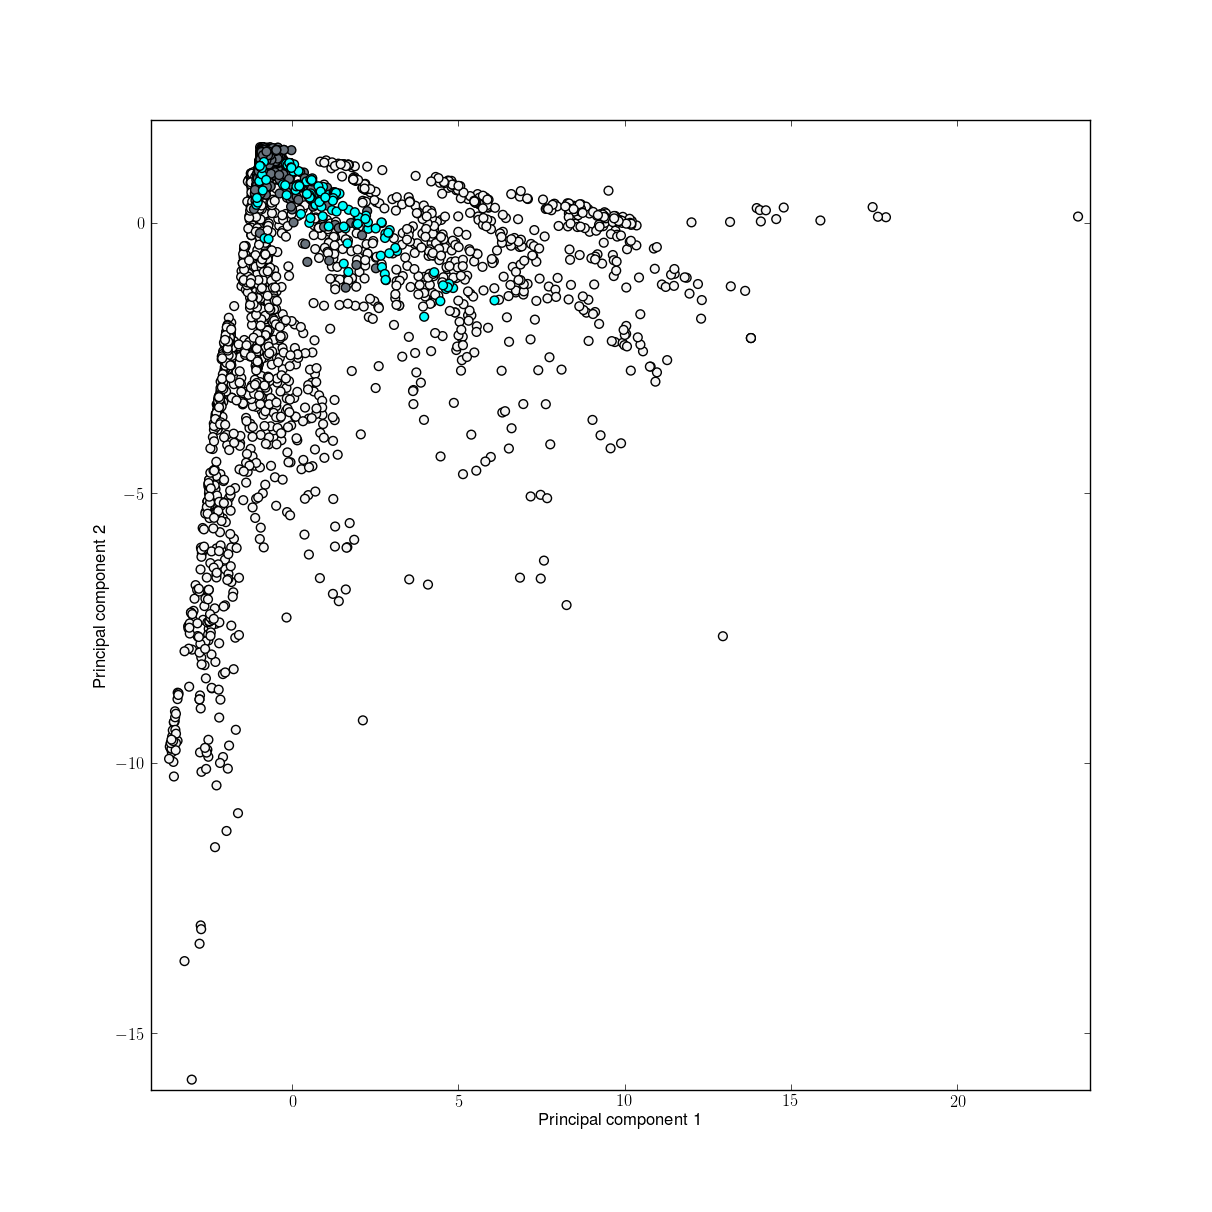
\includegraphics[trim=3cm 3cm 2cm 2cm,clip, width=\textwidth]{./img/pca_visu.png}
	\subcaption{$ACP$}\label{figPCA}
	\end{minipage}
	\begin{minipage}{0.50\textwidth}
	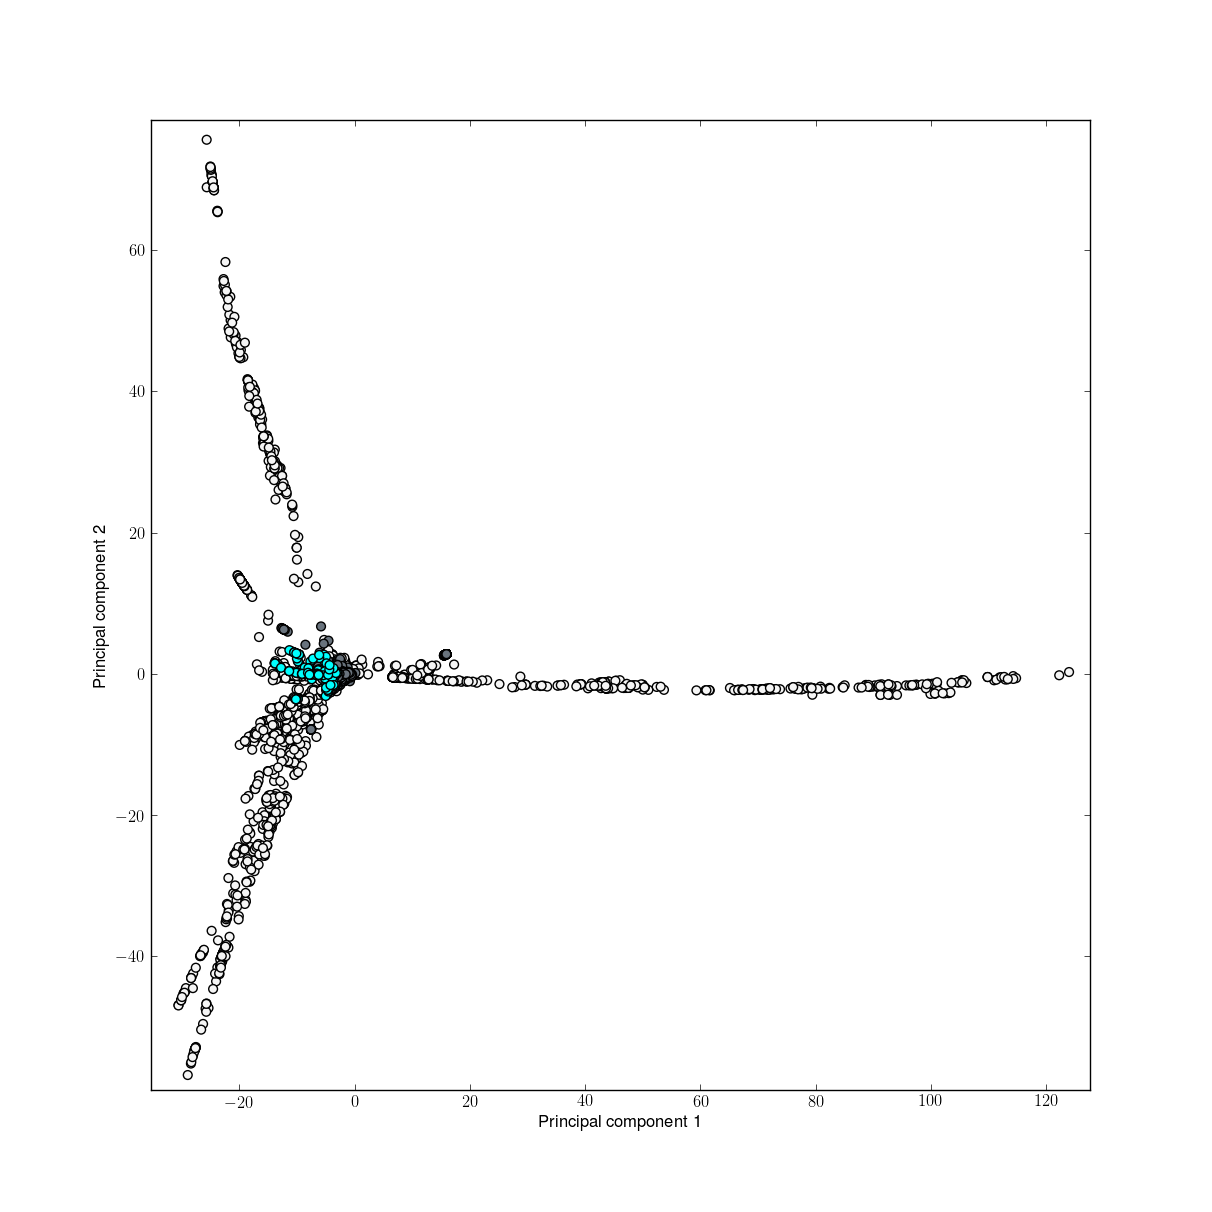
\includegraphics[trim=3cm 3cm 2cm 2cm,clip, width=\textwidth]{./img/ISOMAP.png}
	\subcaption{$ISOMAP$}\label{figISOMAP}
	\end{minipage}
	\\
	\begin{minipage}{0.50\textwidth}
	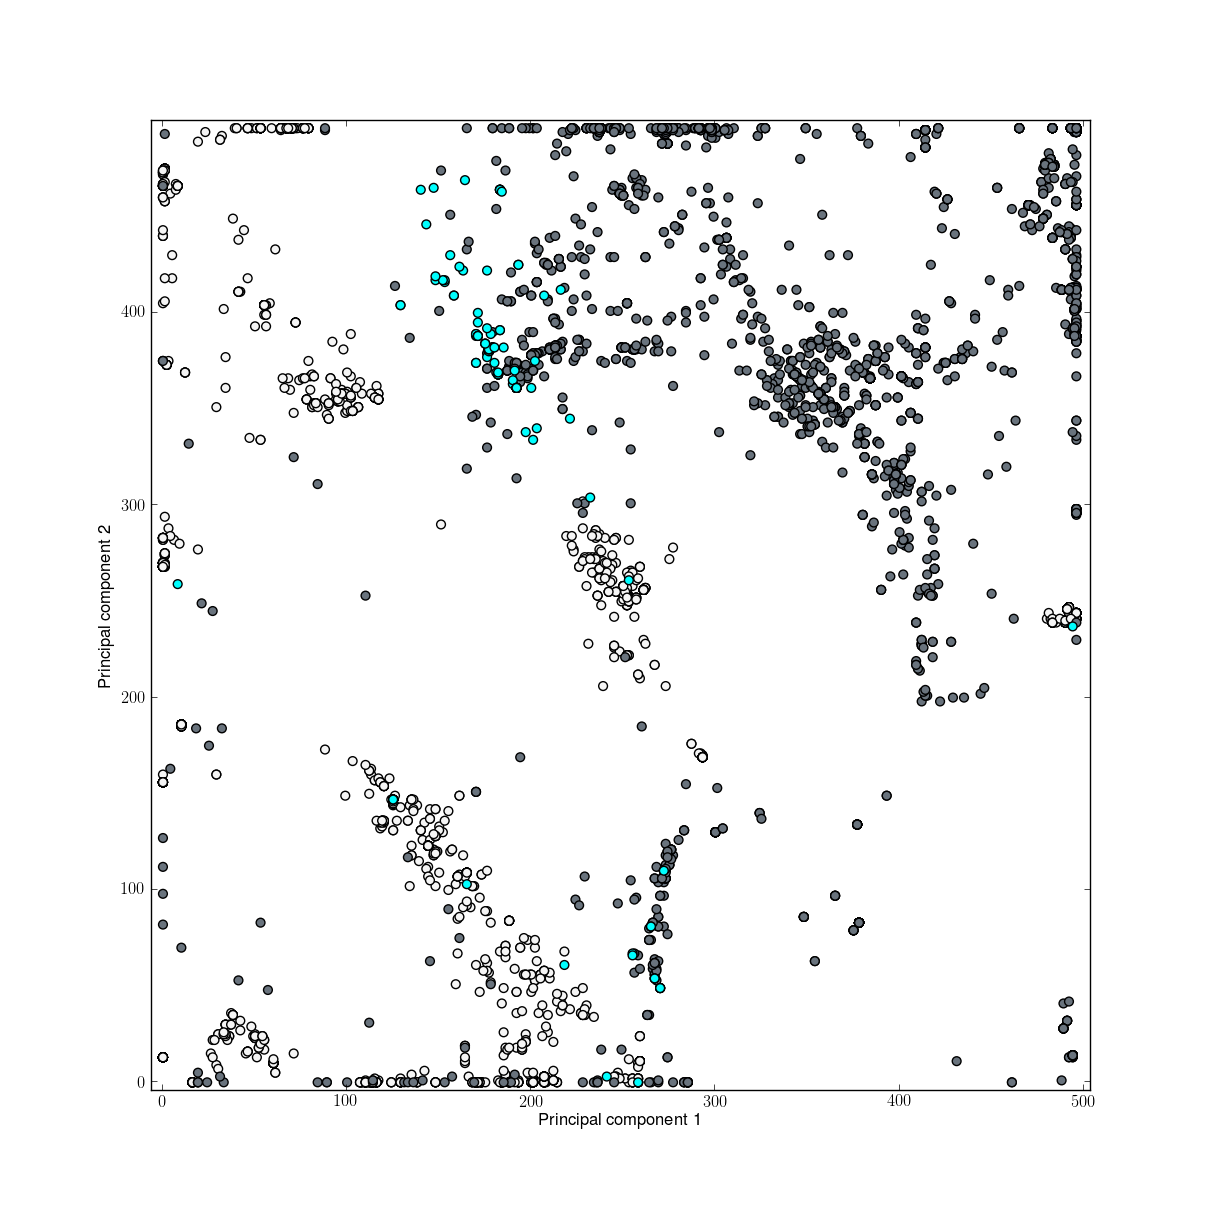
\includegraphics[trim=3cm 3cm 2cm 2cm,clip, width=\textwidth]{./img/SOM2.png}
	\subcaption{$SOM$}\label{figSOM}
	\end{minipage}
	\begin{minipage}{0.50\textwidth}
	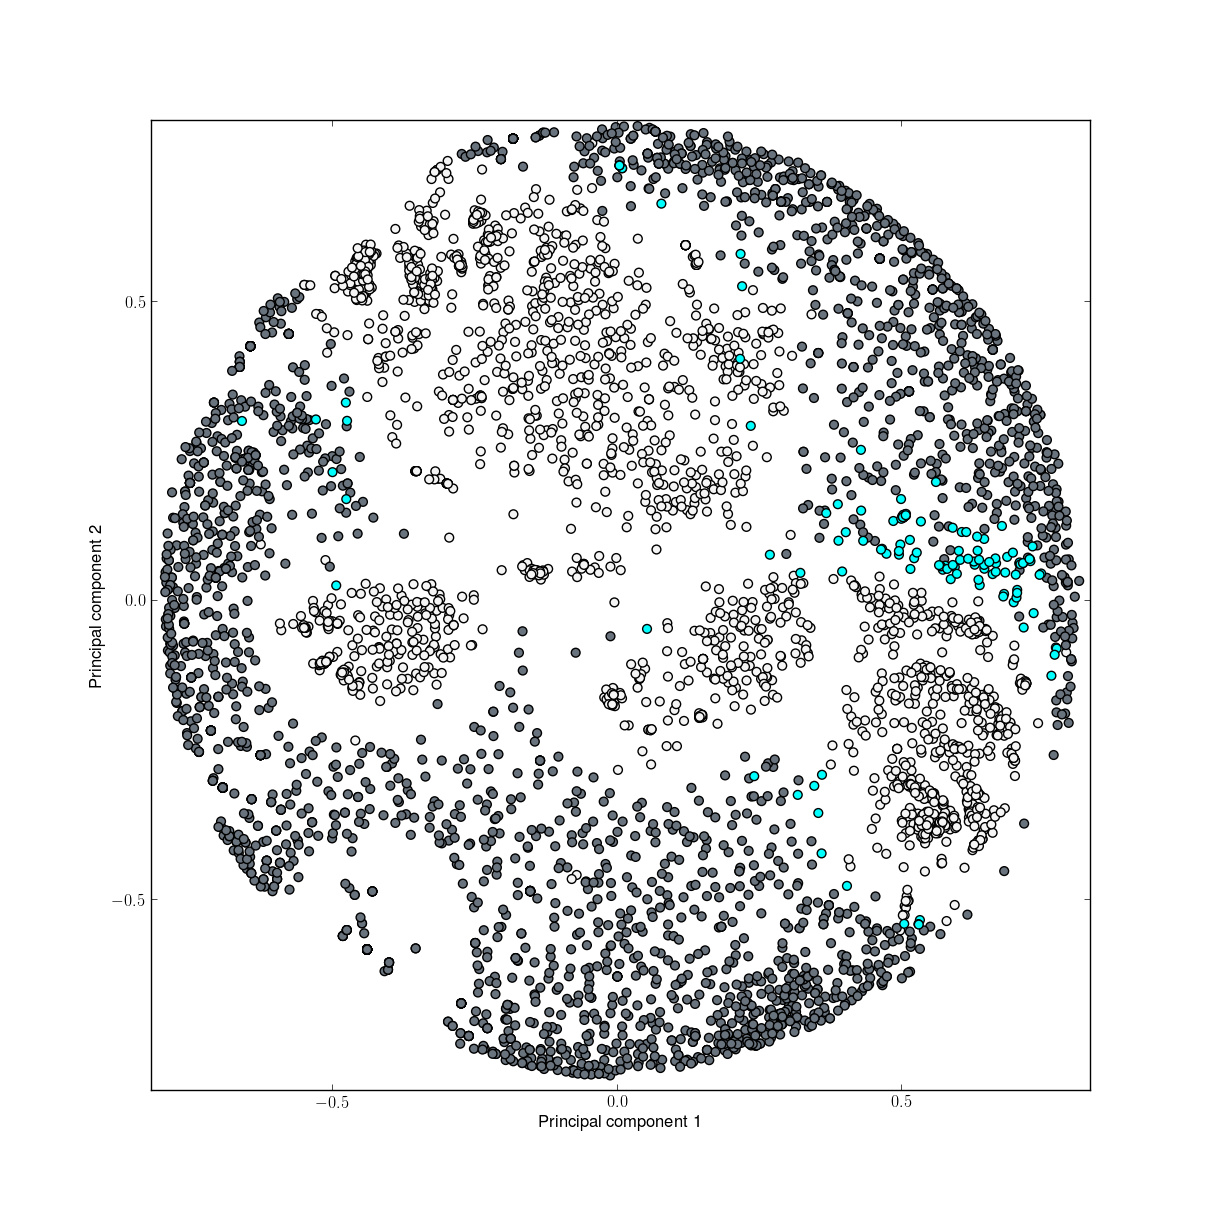
\includegraphics[trim=3cm 3cm 2cm 2cm, clip, width=\textwidth]{./img/MDS_cosine.png}
	\subcaption{$MDS$}\label{figMDS}
	\end{minipage}	

	\caption[Projection de l’ensemble des réplicons]{Projection de l’ensemble des réplicons $V^{R}$\\ \medskip Coloration selon le type de réplicon: chromosome (gris clair), plasmide (gris foncé), RECE (bleu).} 
\end{figure}  

Les algorithmes SOM et MDS produisent une organisation cohérente des réplicons bactériens (Table \ref{tabscorevisu}; Figures \ref{figSOM} et \ref{figMDS}). Ils fournissent une meilleure organisation taxonomique des chromosomes que les ACP et ISOMAP, et réussissent à structurer les réplicons plasmidiques (Table \ref{tabscorevisu}). La distance \textit{cosine}, utilisée par les deux méthodes SOM et MDS, ne tient compte que des attributs non-nuls des observations, et produit des distances pertinentes entre plasmides et chromosomes ainsi qu’entre plasmides. Cette structuration n'est de plus pas influencée par le biais d’échantillonnage des données car elle est également observée sur $\bar{V}^{R}_{genre}$ Figures \ref{figSOMnorm} et \ref{figMDSnorm}). 
 
\begin{figure}[H]
	\begin{minipage}{0.50\textwidth}
	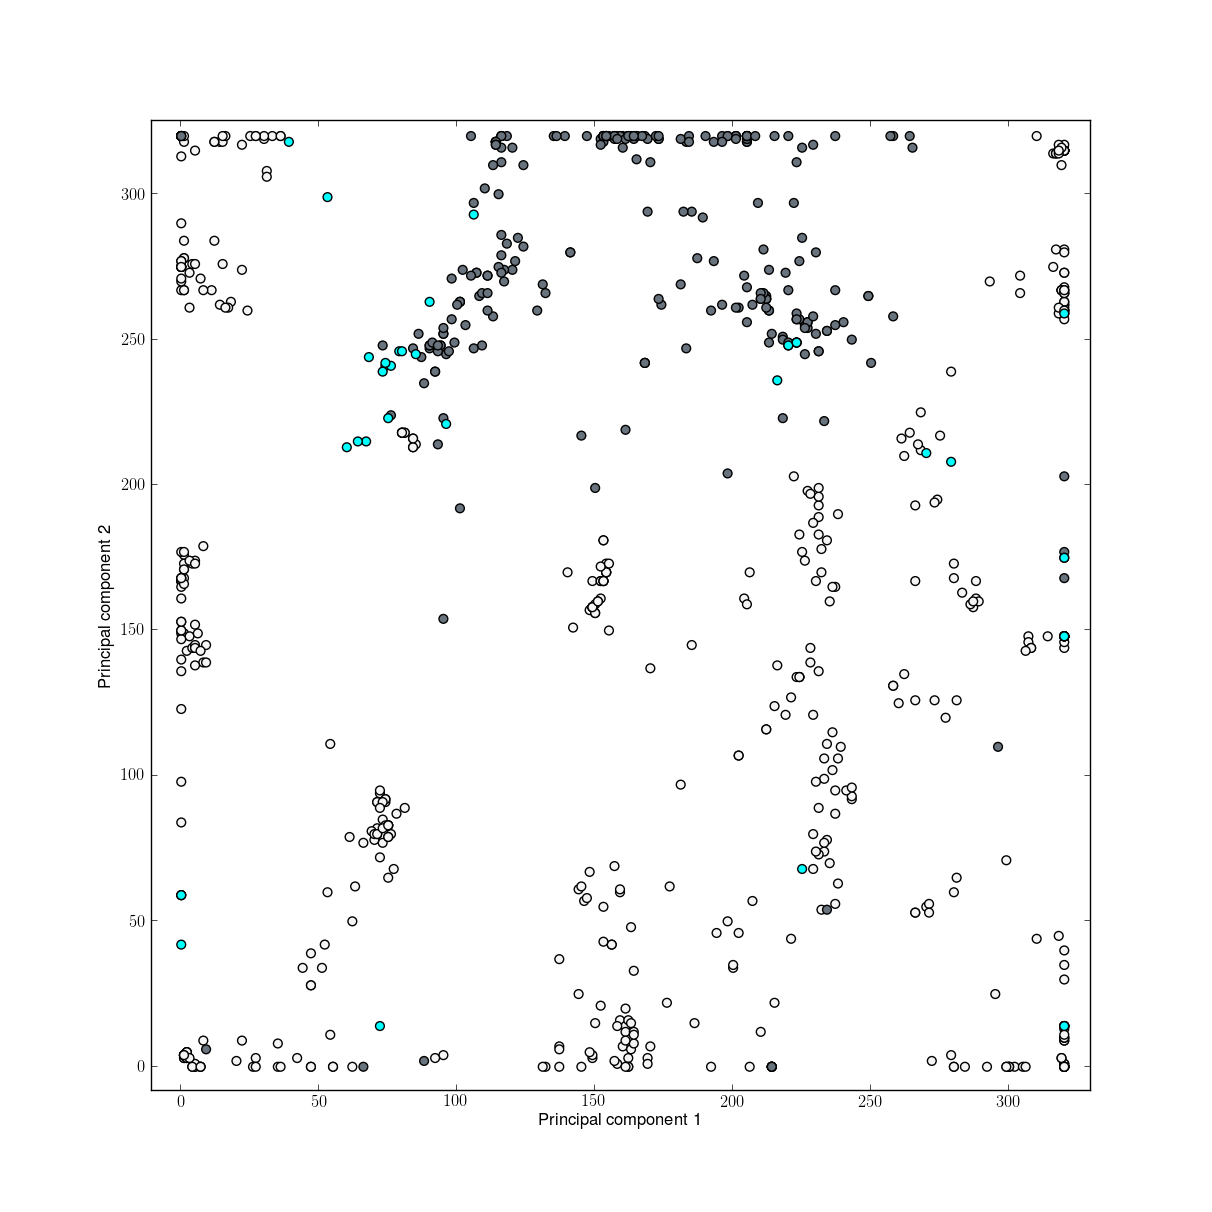
\includegraphics[trim=3cm 3cm 2cm 2cm,clip,width=\textwidth]{./img/SOM_norm.png}
	\subcaption{$SOM$ sur $\bar{V}^{R}_{genre}$}\label{figSOMnorm}
	\end{minipage}
	\begin{minipage}{0.50\textwidth}
	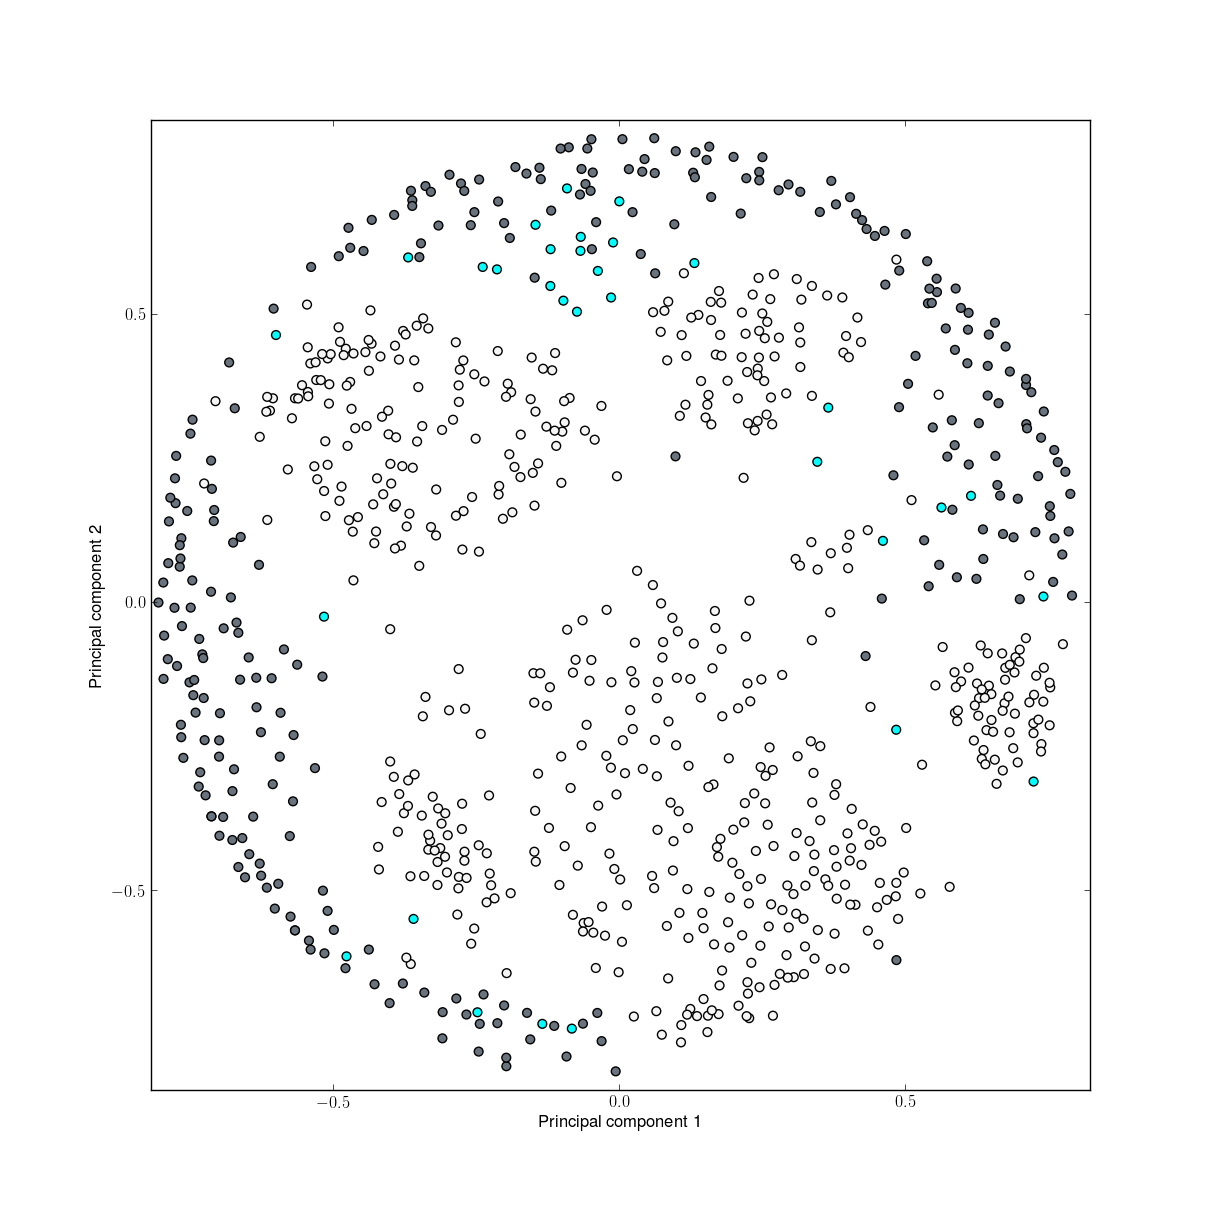
\includegraphics[trim=3cm 3cm 2cm 2cm,clip, width=\textwidth]{./img/MDS_cosine_norm.png}
	\subcaption{$MDS$ sur $\bar{V}^{R}_{genre}$}\label{figMDSnorm}
	\end{minipage}
	\caption[Projection des réplicons normés par genre bactérien]{Projection des réplicons normés par genre bactérien $\bar{V}^{R}_{genre}$\\\medskip Coloration selon le type de réplicon : chromosome (gris clair), plasmide (gris foncé), RECE (bleu).}
\end{figure}  

En prenant un ensemble de cellules $D$ assez large, la SOM parvient à discriminer les plasmides entre eux. Cependant un désavantage non négligeable de la SOM par rapport au MDS est le nombre d'itérations nécessaire (60.000), donc un temps de calcul conséquent, pour produire des résultats robustes.
\\
Concernant les RECE, on peut observer que:
\begin{description}
\item[$\blacktriangleright$] \textbf{\color{orange}Les RECE se placent généralement au niveau de l'interface entre chromosomes et plasmides} et semblent donc posséder des caractéristiques spécifiques les distinguant des plasmides (Figures \ref{figSOM}, \ref{figMDS}, \ref{figSOMnorm} et \ref{figMDSnorm}).
\item[$\blacktriangleright$] \textbf{\color{orange} Quelques RECE montrent une proximité singulière avec les chromosomes.}
\item[$\blacktriangleright$] Même si la séparation plasmide/chromosome est nette, il semble exister une proximité entre les plasmides et les chromosomes dont les hôtes appartiennent au même groupe taxonomique, par exemple, pour des groupes tel que les alpha-, bêta- ou gamma-protéobactéries (Figures \ref{figSOM2} et \ref{figMDS2}).

\begin{figure}[H]		
	\begin{minipage}{0.50\textwidth}		 	
	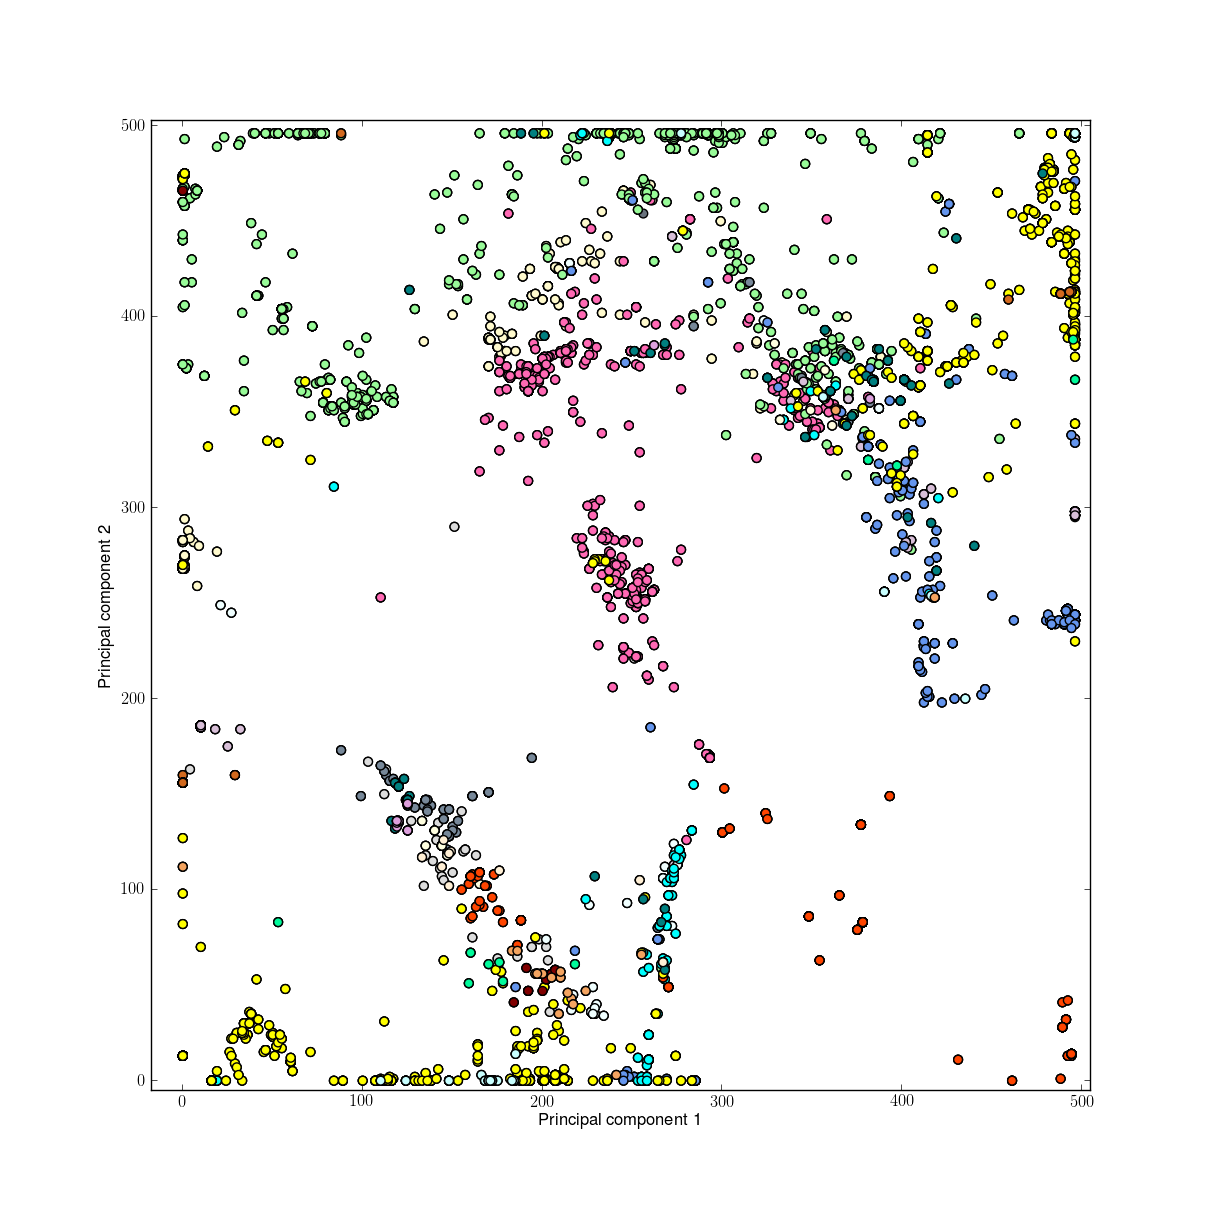
\includegraphics[trim=4cm 3cm 2cm 2cm,clip, width=\textwidth]{./img/SOM2_taxa.png}
	\subcaption{$SOM (2)$}\label{figSOM2}
	\end{minipage}
	\begin{minipage}{0.50\textwidth}
	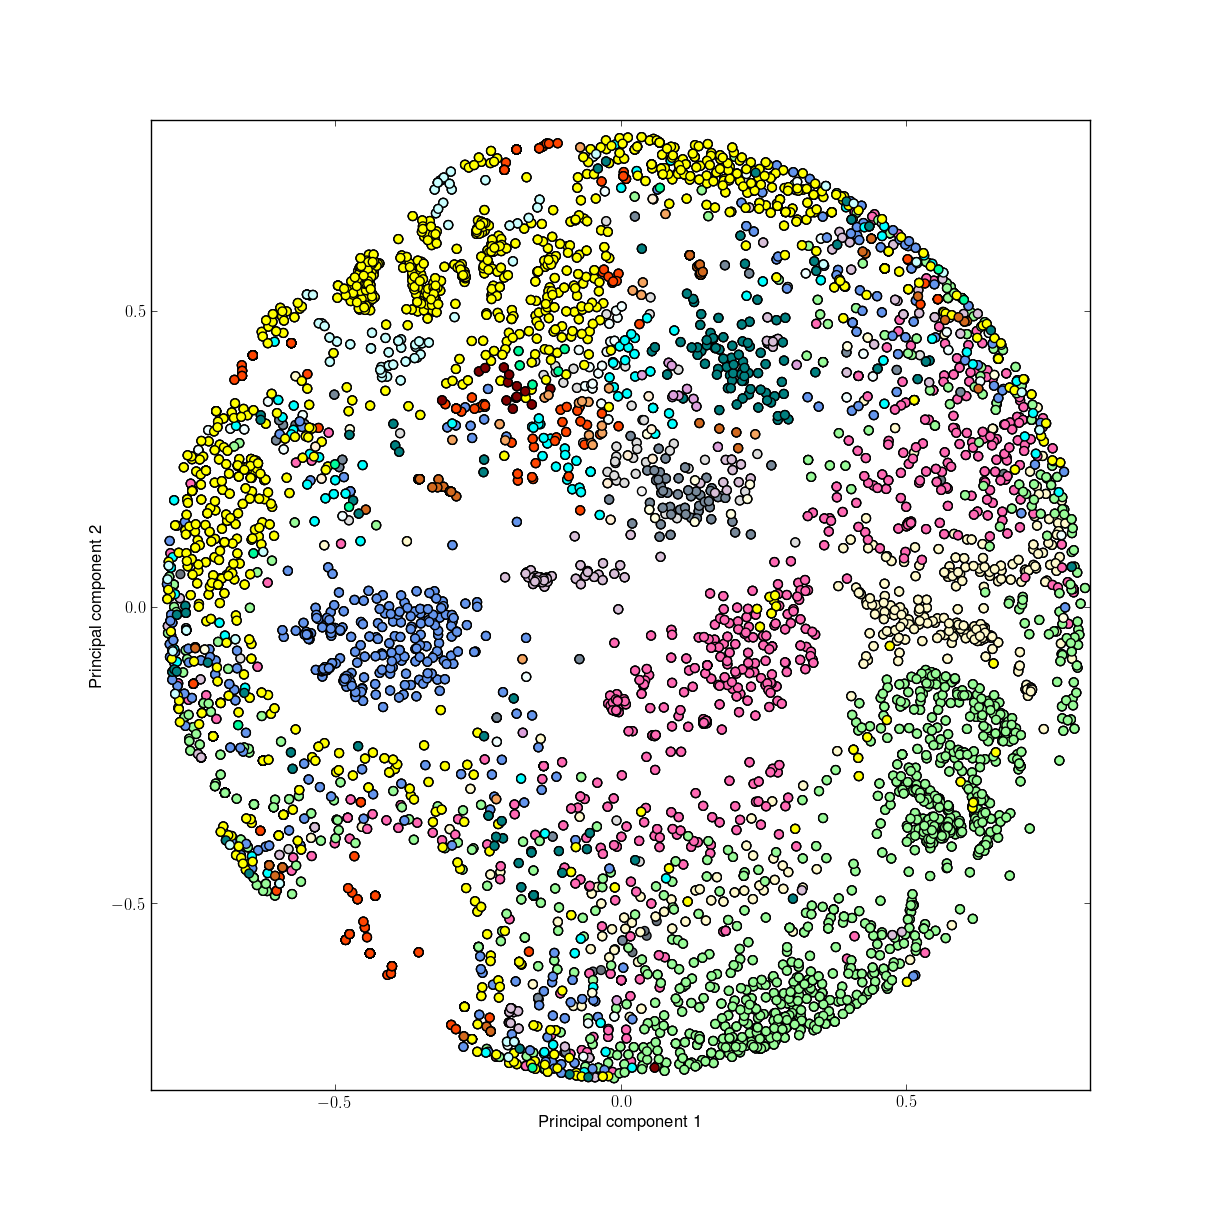
\includegraphics[trim=4cm 3cm 2cm 2cm,clip, width=\textwidth]{./img/MDS_taxa.png}
	\subcaption{$MDS (2)$}\label{figMDS2}
	\end{minipage}
	\caption[Identification des lignées bactériennes sur la projection des réplicons]{Représentation des lignées bactériennes sur les projections de l’ensemble des réplicons $V^{R}$ \\\medskip  Coloration selon la taxonomie de la bactérie-hôte : Acidobactéries (jaune transparent), Actinobactéries (bleu), Bacteroidetes (vert émeraude), Chlamydiae (orange foncé), Chlorobi (rose pâle), Chloroflexi (orange pâle), Cyanobactéries (cyan), Deinococcus-Thermus (bleu transparent), Firmicutes (jaune), Fusobactéries (vert), Planctomycètes (beige clair), Protéobacteries: Alpha (rose), Bêta (jaune pâle), Delta (gris foncé), Epsilon (violet pâle), et Gamma (vert clair), Spirochètes (rouge), Ténéricutes (bleu pâle), Thermotogae (marron foncé), Autres (gris pâle).}
\end{figure}  

\item[$\blacktriangleright$] \textbf{Cette proximité entre chromosomes et plasmides d'un même groupe taxonomique témoigne du flux intra-génomique de gènes liés aux STIG entre plasmides et chromosomes.}
\end{description}   

 \subsection{Graphes}
	En utilisant l'éq. \ref{eqbipartite}, $V^{R}$ et $\bar{V}_{genre}^{R}$ sont transformés en graphes bipartites, qui sont ensuite visualisés par des techniques dédiées de visualisation des graphes. Elles consistent à représenter les nœuds et arcs/arêtes des graphes par des points et flèches/traits entre les points dans un espace à deux ou trois dimensions. L’épaisseur des traits peut être une fonction de la pondération. Des algorithmes de topologie ou \textit{layout} organisent la  disposition des nœuds dans l'espace selon différentes stratégies. L’une d’entre elles est le \textit{force-directed layout} où un système de forces est appliqué à chaque nœud en fonction de ses arêtes. Le graphe est alors mis en mouvement jusqu'à ce qu'il atteigne un état stable. Ce  dernier dépend de la connectivité inter-nœud et peut être assimilé, par analogie, à l'action d'un champ de force (gravité, interaction électrostatique,...) sur une molécule, lui faisant adopter sa configuration la plus stable. L'algorithme que nous avons employé pour visualiser nos graphes est \textit{ForceAtlas2} \citep{jacomy2011forceatlas2}.
	%Dans un deuxième temps, $V^{R}$ et $\bar{V}_{genre}^{R}$ sont transformé en graphes bipartites en utilisant l'éq. \ref{eqbipartite}. Les graphes obtenus sont ensuite visualisées en utilisant les techniques de visualisation des graphes. Ces techniques consiste à représenter les nœuds et arcs/arêtes des graphes généralement par des points et flèches/traits entre les points dans un espace en 2 ou 3 dimensions, leur épaisseur pouvant être une fonction de leur pondération. La visualisation des graphes consiste à utiliser des algorithme de topologie ou \textit{layout}   organisant disposition des nœuds  dans l'espace selon différentes stratégies. Une de ces stratégies sont les \textit{force-directed layout} où un système de forces est appliqué à chaque noeud en fonctions de ses arêtes. Le graphe est alors mis en mouvement jusqu'à ce qu'il atteigne un état stable. Cet état stable dépend de la \textit{connectivité} inter-noeud et peut être assimilé, par analogie, à l'action d'un champ de force (gravité, interaction électrostatique,...) sur une molécule lui faisant adopter la configuration dans laquelle celle-ci est la plus stable. L'algorithme utilisée dans la visualisation des graphes est \textit{ForceAtlas2} \citep{jacomy2011forceatlas2}.  
		
\subsubsection{Graphes: résultats}\label{graphres}
	L'analyse des graphes formés pour $V^{R}$ (Figure \ref{figgrapherepl}) et des sous-graphes des différents groupes taxonomiques contenant des espèces multipartites (Figure \ref{figgprahe2}) apporte un autre point de vue que les projections en permettant d'analyser plus précisément les différentes interconnections de chaque réplicon par rapport aux clusters de protéines. L'utilisation du logiciel de visualisation Gephi, par ses nombreuses fonctionnalités, a apporté une contribution non négligeable dans la fouille de données des graphes.\\

 La quasi-majorité des réplicons sont interconnectés, témoignant de l'hérédité partagée des gènes des STIG présents dans les génomes bactériens. Plasmides et chromosomes semblent cependant clairement appartenir à des communautés différentes. Il existe néanmoins pour certains phyla une interconnection forte entre chromosomes et plasmides. Est passé en revue ci-dessous les observations tirées de l'analyse des graphes pour les génomes multipartites. À cause de la grande complexité des données, seulement les observations les plus marquantes visuellement sont rapportées. 
 
 \begin{description}
 \item[Protéobactéries] Différents niveaux de connections des RECE avec les plasmides et chromosomes existent chez les protéobactéries (détaillés ci-dessous). Les RECE des Protéobactéries sont interconnectés \textit{via} certains clusters remarquables, notamment les clusters annotés IciA, Lrp, FtsE, AcrA ou HN-S (Figure \ref{figconnectiv}). De manière générale, les RECE fortement interconnectés avec les plasmides le sont \textit{via} les clusters annotés ParA/ParB, Rep et en lien avec les systèmes PSK.

 	\begin{itemize}
 	\item[\textbf{Alpha}] Les RECE sont liés pour part à de nombeux clusters plasmidiques dont ceux annotés ParA, ParB et RepC, témoignant de la proximité avec les plasmides de type RepABC présents chez les Alphaprotéobactéries. Cependant, ilsi sont liés à des clusters typiquement chromosomiques, FtsK (pour les RECE de \textit{Brucella} et d'\textit{Agrobacterium}) et ParE (pour les RECE de \textit{Brucella}) notamment. Il existe des clusters spécifiques des RECE, annotés TyrK, FtsE ou AcrA particulièrement. Enfin, l'interconnection des RECE de \textit{Paracoccus} et de \textit{Asticcacaulis} avec des réplicons chromosomiques est surprenante (Figure \ref{figalpha}). Les RECE des \textit{Brucella} forment un groupe distinct alors que ceux de \textit{Sphingobium} semblent plus interconnectés avec des plasmides.
 	% Les gènes des STI suggérés comme étant transférés entre le chromosome et les plasmides ancestrales des Rhizobiales \citep{Slater2009} sont retrouvés sur les RECE correspondant. 
 	\item[\textbf{Bêta}] Les RECE se distinguent clairement des chromosomes et des plasmides en formant un groupe homogène distinct (Figure \ref{figbeta}). Ils partagent différents clusters avec les plasmides tels que ceux annotés parA ou Xer, entre autres. Les RECE sont interconnectés aux chromosomes \textit{via} de nombreux clusters tels que FtsI, IciA ou Rob. Il existe des différences entre les RECE I et les RECE II des \textit{Burkholderia}, ces derniers semblant plus interconnectés aux plasmides.Il est à noter que les RECE I des \textit{Burkholderia} sont liés à des clusters annotés DnaG connectés aux chromosomes (sauf ceux des \textit{Burkholderia}), témoignant d'un probable transfert ancestral du chromosome vers le RECE I. 
 	\item[\textbf{Gamma}] Les RECE sont connectés à l'interface des chromosomes et plasmides (Figure \ref{figgamma}). Ceux de \textit{Pseudoalteromonas} sont moins interconnectés avec les RECE des \textit{Vibrio/Aliivibrio} et \textit{Photobacterium} soulignant leur origine distincte.
 	\end{itemize}
\item[Acidobactéries] Le RECE de \textit{Candidatus} Chloroacidobacterium thermophilum est interconnecté aux chromosomes par ParA/ParB, DnaB, AcrA, ScpB principalement, et n'est pas interconnecté avec les plasmides des Acidobactéries. Il est cependant connecté à des plasmides d'autres phylum \textit{via} des clusters Rep, Helicase ou PSK principalement.
 \item[Actinobactéries] Le RECE de \textit{Nocardiopsis dassonvillei} est interconnecté aux chromosomes \textit{via} de nombreux clusters annotés principalement FtsE, FtsK, FtsW, FtsI, MinD et ParA.
 \item[Bacteroidetes] Les RECE de \textit{Prevotella} sont interconnectés aux chromosomes \textit{via} de très nombreux clusters et ont peu d'interconnections avec les plasmides.
 \item[Chloroflexi] Les RECE de \textit{Sphaerobacter thermophilus} et \textit{Thermobaculum terrenum} sont interconnectés aux chromosomes et aux plasmides \textit{via} de nombreux clusters. En particulier, le RECE de \textit{S. thermophilus} est lié aux clusters DnaA (GI: 269929006), DnaG et FtsI. 
 \item[Cyanobactéries] Deux configurations distinctes sont trouvées chez les RECE de \textit{Anabaena} et \textit{Cyanothece}: le RECE de \textit{Anabaena} est assez interconnecté aux chromosomes \textit{via} des clusters annotés FstI, DnaG, FtsE, CpbA, MreB, ParA entre autre. Inversement le RECE de\textit{Cyaothece} interconnecté aux plasmides \textit{via} des clusters de type Xer, ParA et helicase notamment.
\item[Deinococcus-Thermus] Le RECE de \textit{Deinococcus} est lié à huit clusters annotés ParA, ParB, FtsE, Helicase, XerC et HupB. Par le nombre de clusters et par son interconnection, Il est beaucoup plus proche des autres plasmides de \textit{Deinococcus}. Il est cependant interconnecté aux chromosomes \textit{via} les clusters FtsE et HupB notamment et est lié à un nombre (trois) relativement élevé de cluster FtsE. 
 \item[Firmicutes] Le RECE de \textit{Butyrivibrio proteoclasticus} est connecté aux plasmides \textit{via} des clusters annotés Rep et PSK principalement et est connecté aux chromosomes \textit{via} ceux annotés DnaB, Rob, FtsE, Xer. pCY186, un plasmide de \textit{B. proteoclasticus} est attaché au même cluster DnaB, ainsi qu'à deux clusters annotés DnaA (GI: 302668636 et 302668625).
 \item[Spirochètes] Les RECE de \textit{Leptospira} sont liés chacun à trois ou qutre clusters de protéines pour un total de six clusters différents. Les clusters en commun sont annotés ParA et ParB et ceux n'étant pas présents sur tous les RECE sont annotés XerD et HupB. Le cluster annoté ParA est lié exclusivement aux chromosomes des spirochètes, avec une exception: un plasmide de \textit{Turneriella}. Aucun des six clusters n'est lié à un autre plasmide des Spirochètes. Les RECE possèdent de plus deux gènes appartenant à ce cluster. 
\end{description}  
 
\begin{landscape}
\thispagestyle{plain}
\begin{figure}
\vspace{-2cm}
\hspace{-2cm}
\begin{minipage}[t]{0.5\linewidth}
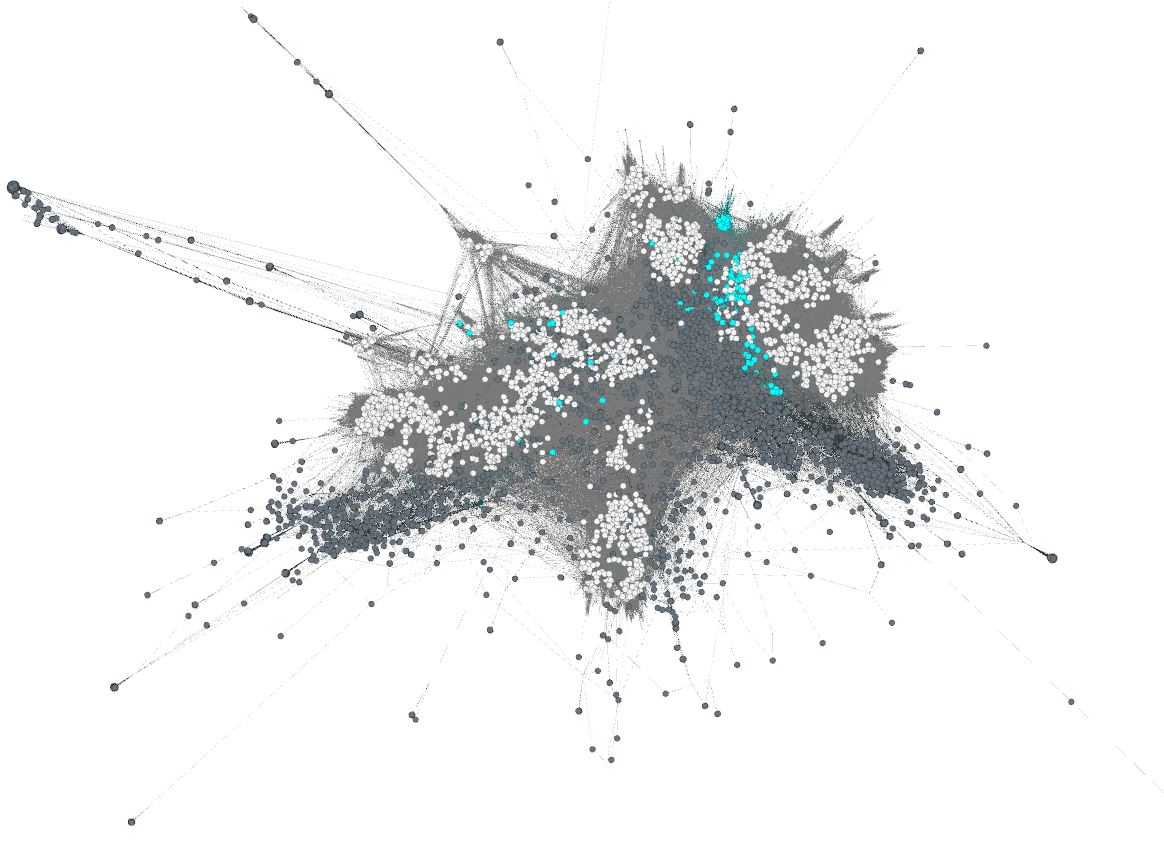
\includegraphics[width=1.13\textwidth ]{./img/graph_all_grey_white_cyan.png}
\subcaption{Type de réplicons}\label{figrepltype}
\end{minipage}
\hspace{1.5cm}
\begin{minipage}[t]{0.5\linewidth}
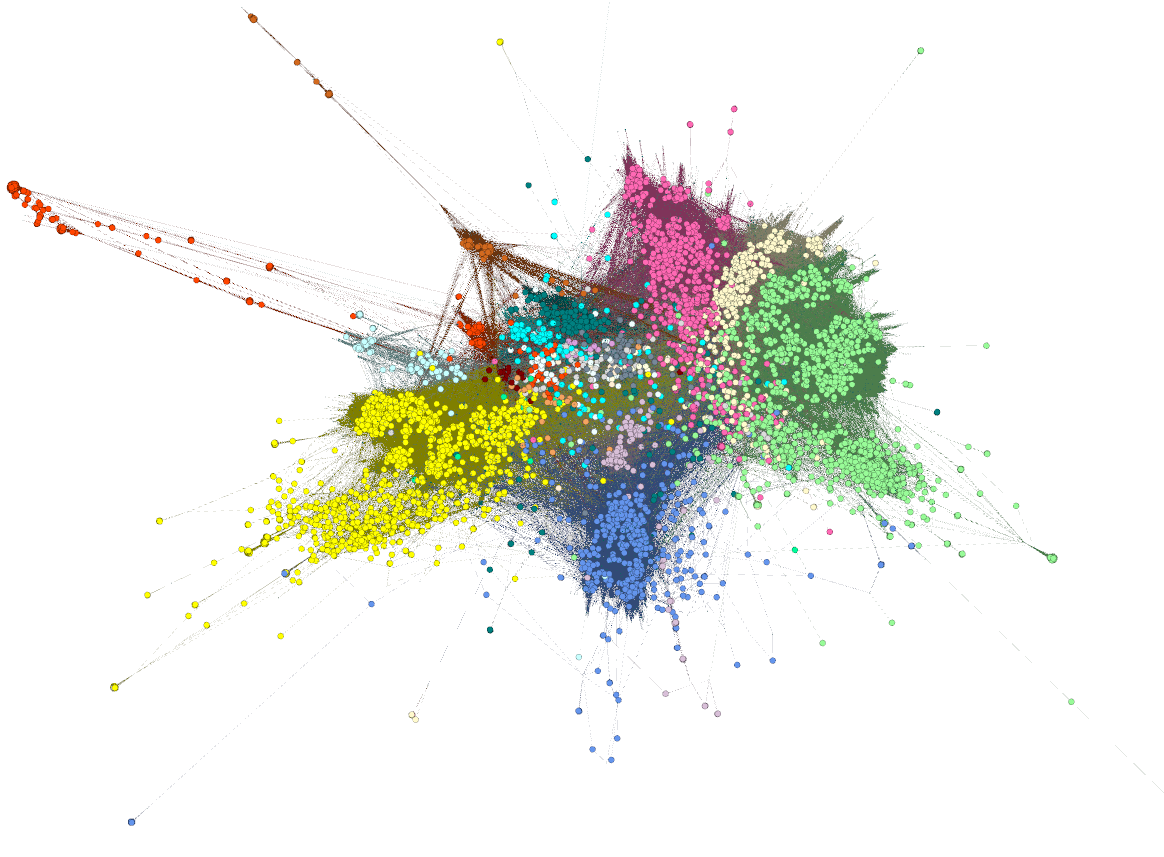
\includegraphics[width=1.13\textwidth ]{./img/graph_all_taxa_color_whitefont.png}
\subcaption{Phylum/Classe des bactéries-hôtes}\label{figreplphyl}
\end{minipage}
\caption[Visualisation des réplicons par graphe bipartite]{Visualisation des réplicons par graphes bipartites.\\\medskip \ref{figrepltype}. Selon le type de réplicon : chromosome (gris clair), plasmide (gris foncé), RECE (bleu). \ref{figreplphyl}. Selon la taxonomie de la bactérie-hôte : Acidobactéries (jaune transparent), Actinobactéries (bleu), Bacteroidetes (vert émeraude), Chlamydiae (orange foncé), Chlorobi (rose pâle), Chloroflexi (orange pâle), Cyanobactéries (cyan), Deinococcus-Thermus (bleu transparent), Firmicutes (jaune), Fusobactéries (vert), Planctomycètes (beige clair), Protéobacteries: Alpha (rose), Bêta (jaune pâle), Delta (gris foncé), Epsilon (violet pâle), et Gamma (vert clair), Spirochètes (rouge), Ténéricutes (bleu pâle), Thermotogae (marron foncé), Autres (gris pâle).}\label{figgrapherepl}
\end{figure}
\end{landscape}


\begin{landscape}
\thispagestyle{empty}
\begin{figure}
\vspace{-3cm}
\begin{center}
\begin{minipage}[t]{0.40\textwidth}
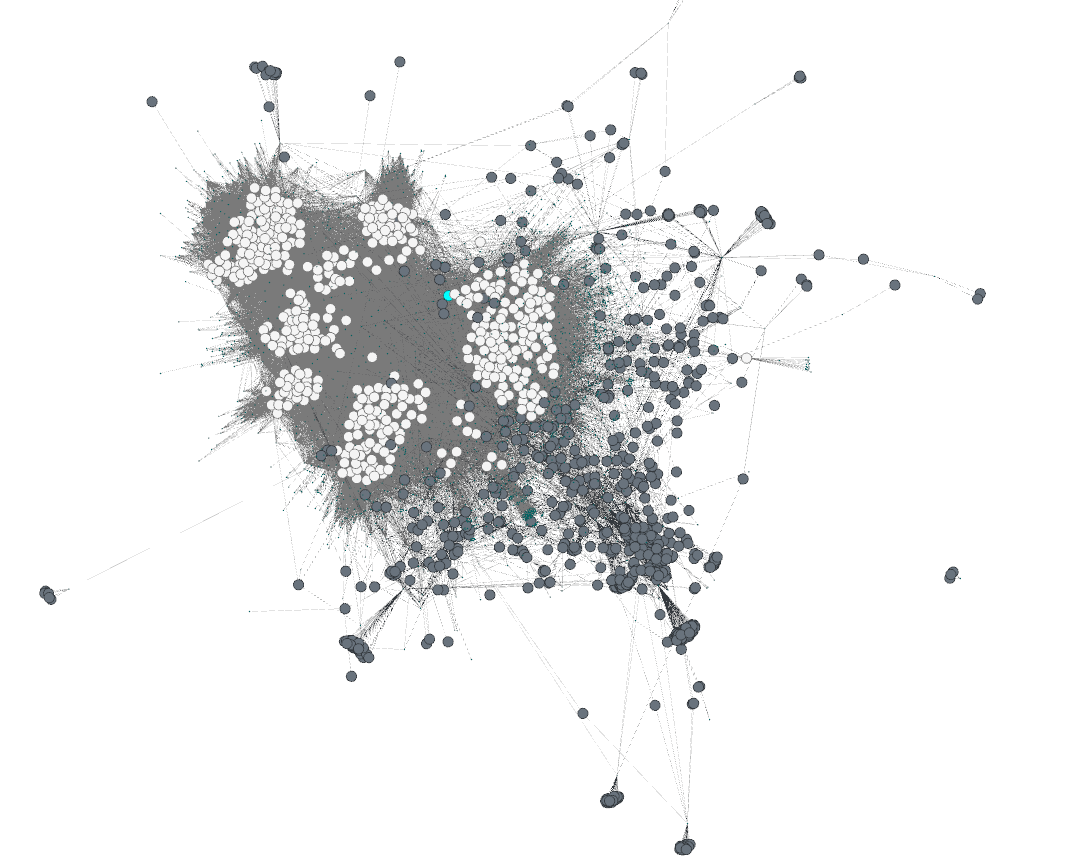
\includegraphics[width=\textwidth]{./img/clostrid.png}
\subcaption{Firmicutes}\label{figclost}
\end{minipage}
\begin{minipage}[t]{0.40\textwidth}
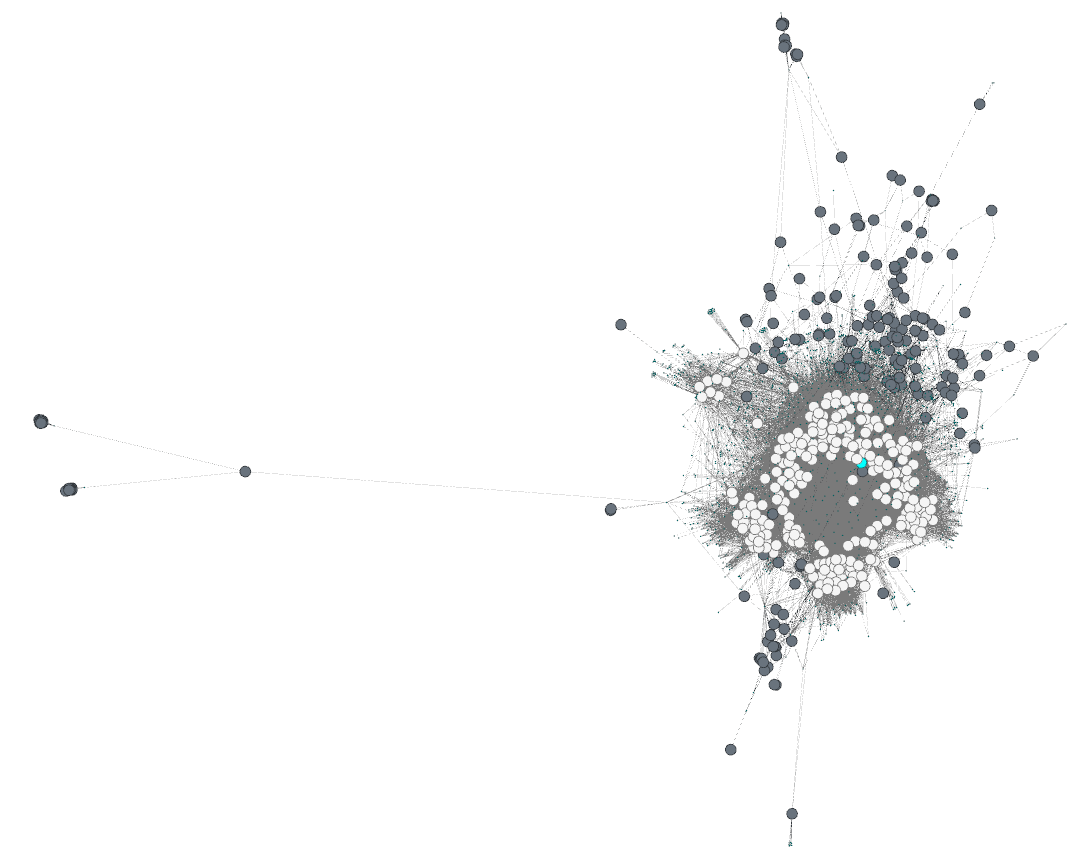
\includegraphics[width=\textwidth]{./img/actinobacter.png}
\subcaption{Actinobactéries}\label{figactino}
\end{minipage}
\begin{minipage}[t]{0.40\textwidth}
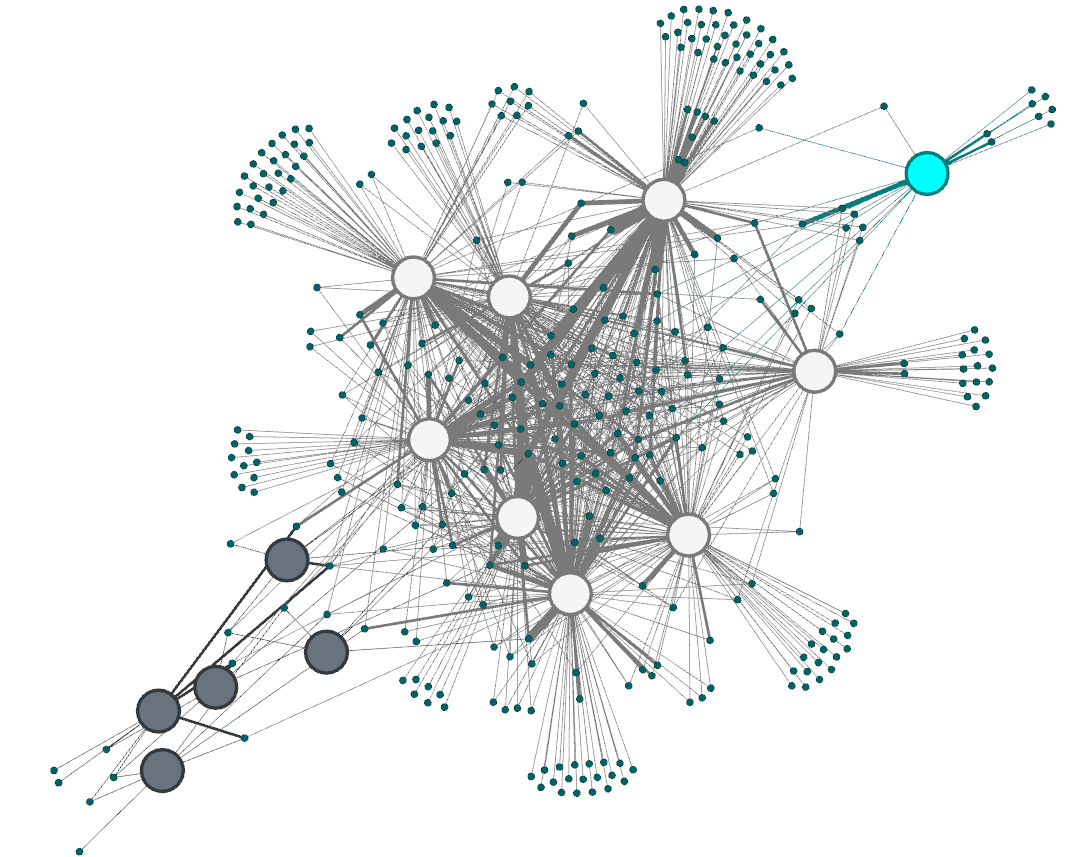
\includegraphics[width=\textwidth]{./img/acido.png}
\subcaption{Acidobactéries}\label{figacido}
\end{minipage}
\begin{minipage}[t]{0.40\textwidth}
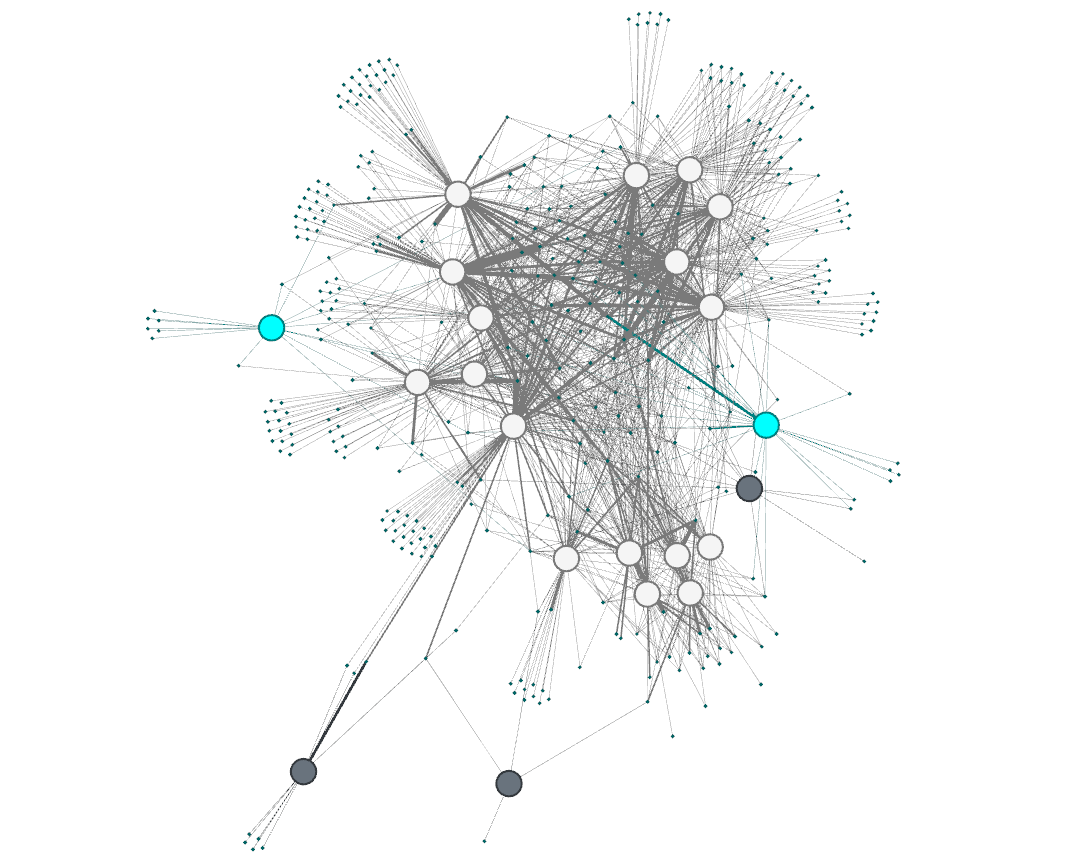
\includegraphics[width=\textwidth]{./img/chloroflex.png}
\subcaption{Chloroflexi}\label{chloro}
\end{minipage}
\\
\vspace{0.2cm}
\begin{minipage}[t]{0.40\textwidth}
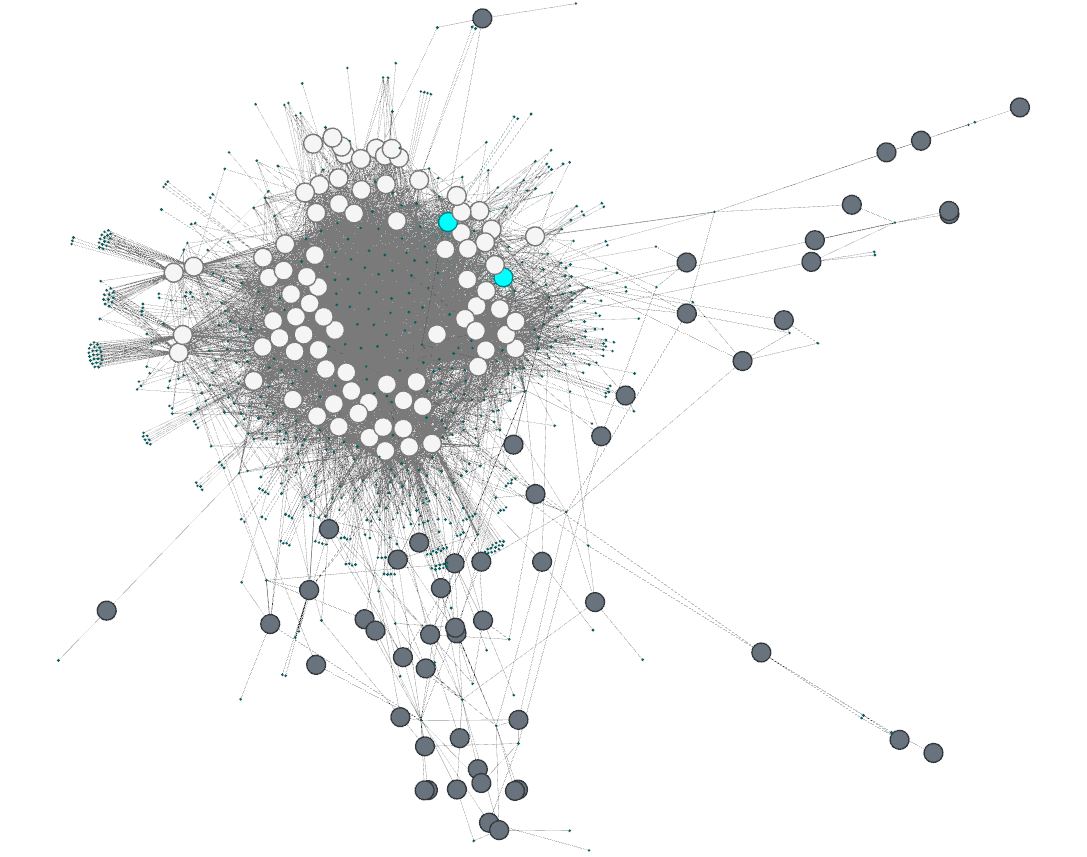
\includegraphics[width=\textwidth]{./img/BCF.png}
\subcaption{Bacteroidetes}\label{figbact}
\end{minipage}
\begin{minipage}[t]{0.40\textwidth}
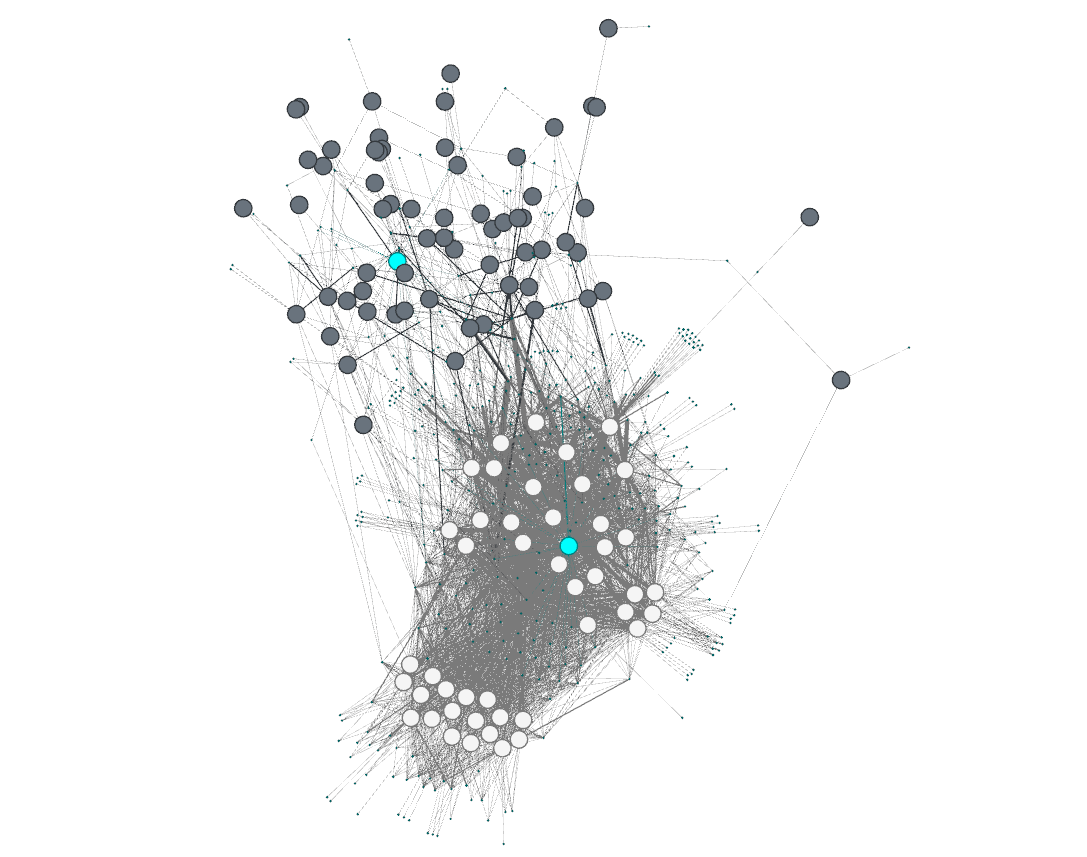
\includegraphics[width=\textwidth]{./img/cyano.png}
\subcaption{Cyanobactéries}\label{figcyano}
\end{minipage}
\begin{minipage}[t]{0.40\textwidth}
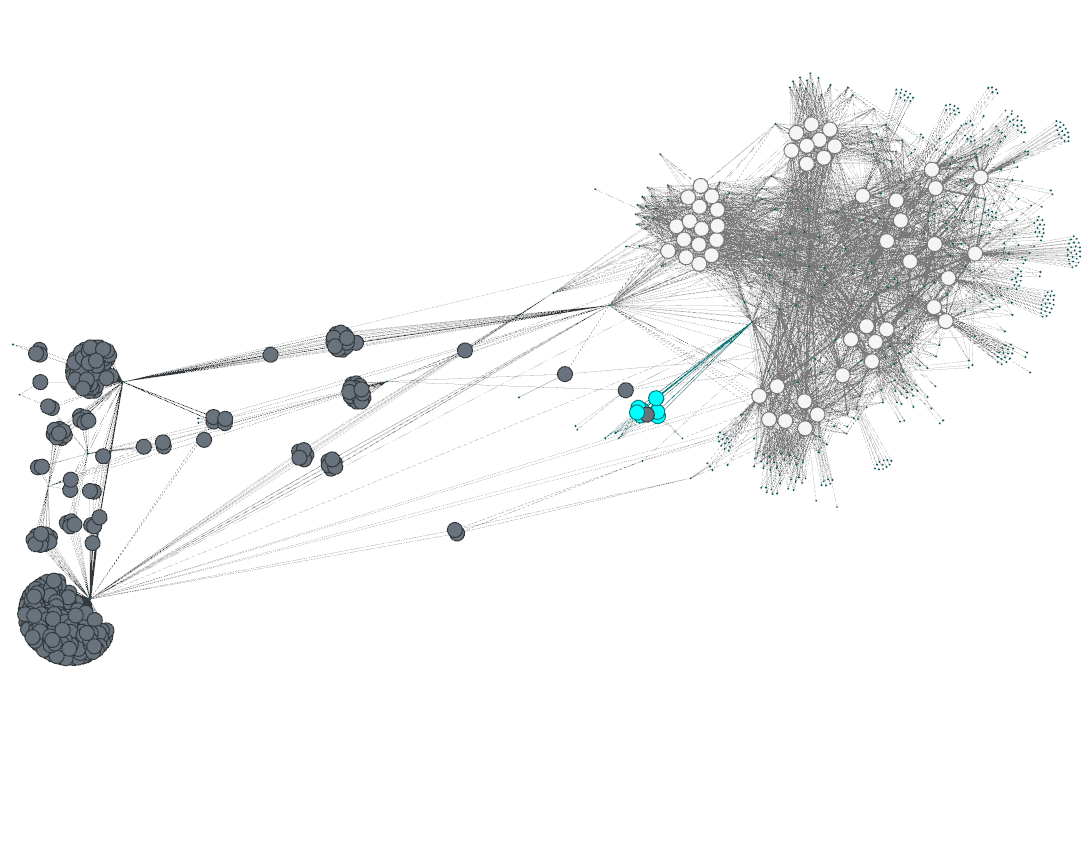
\includegraphics[width=\textwidth]{./img/leptospir.png}
\subcaption{Spirochètes}\label{figspiro}
\end{minipage}
\begin{minipage}[t]{0.40\textwidth}
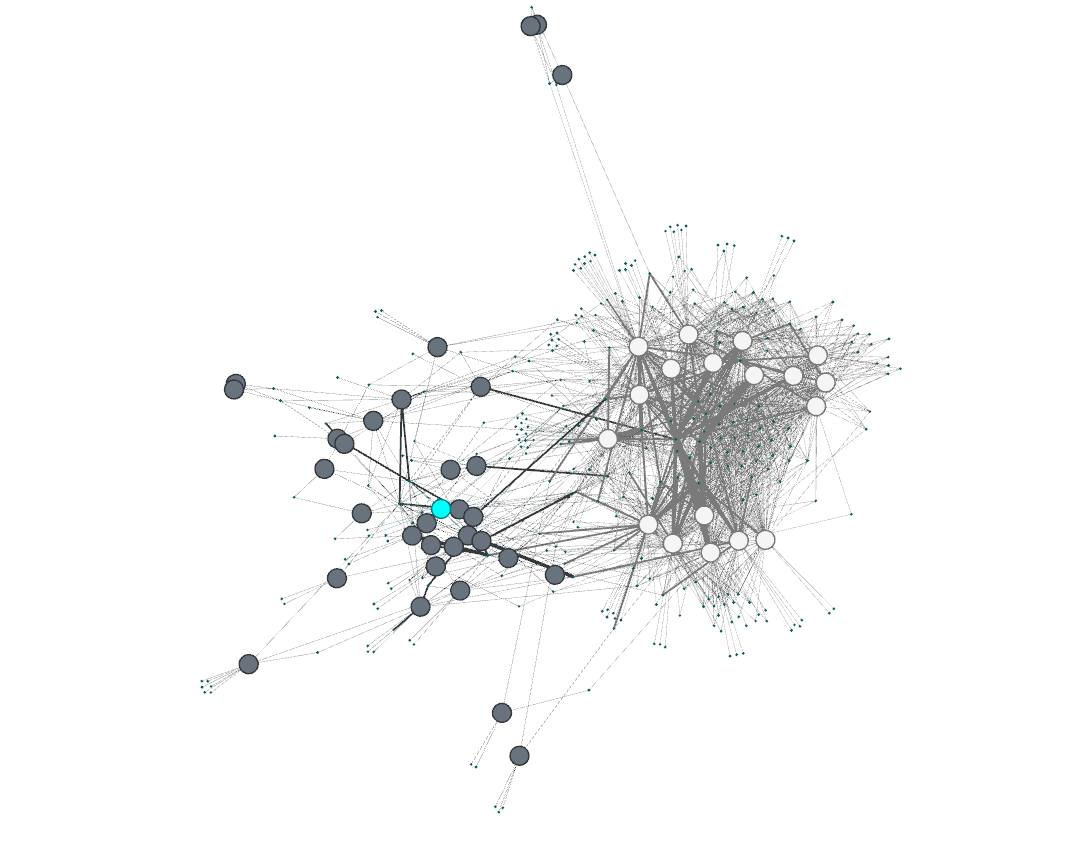
\includegraphics[width=\textwidth]{./img/deinococcus.png}
\subcaption{Deinococcus-Thermus}\label{figdeino}
\end{minipage}
\\
\vspace{0.2cm}
\begin{minipage}[t]{0.40\textwidth}
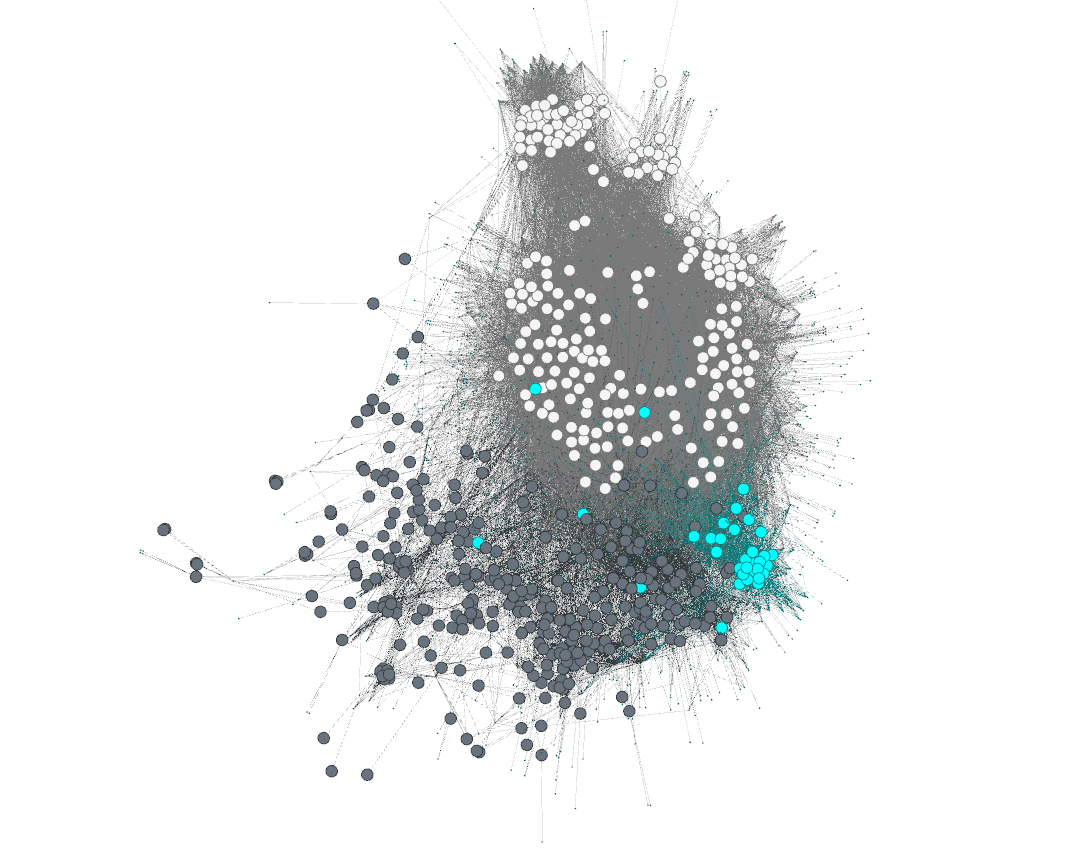
\includegraphics[width=\textwidth]{./img/alpha.png}
\subcaption{Alphaprotéobactéries}\label{figalpha}
\end{minipage}
\begin{minipage}[t]{0.40\textwidth}
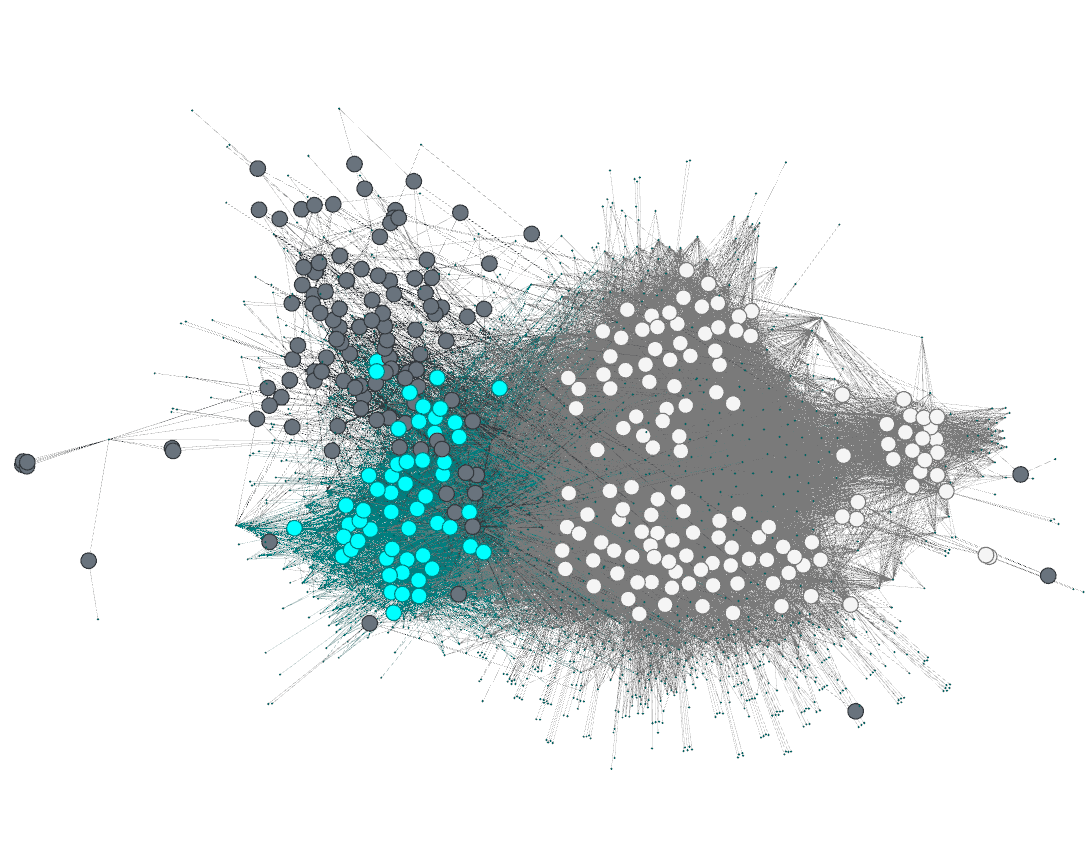
\includegraphics[width=\textwidth]{./img/beta.png}
\subcaption{Bêtaprotéobactéries}\label{figbeta}
\end{minipage}
\begin{minipage}[t]{0.40\textwidth}
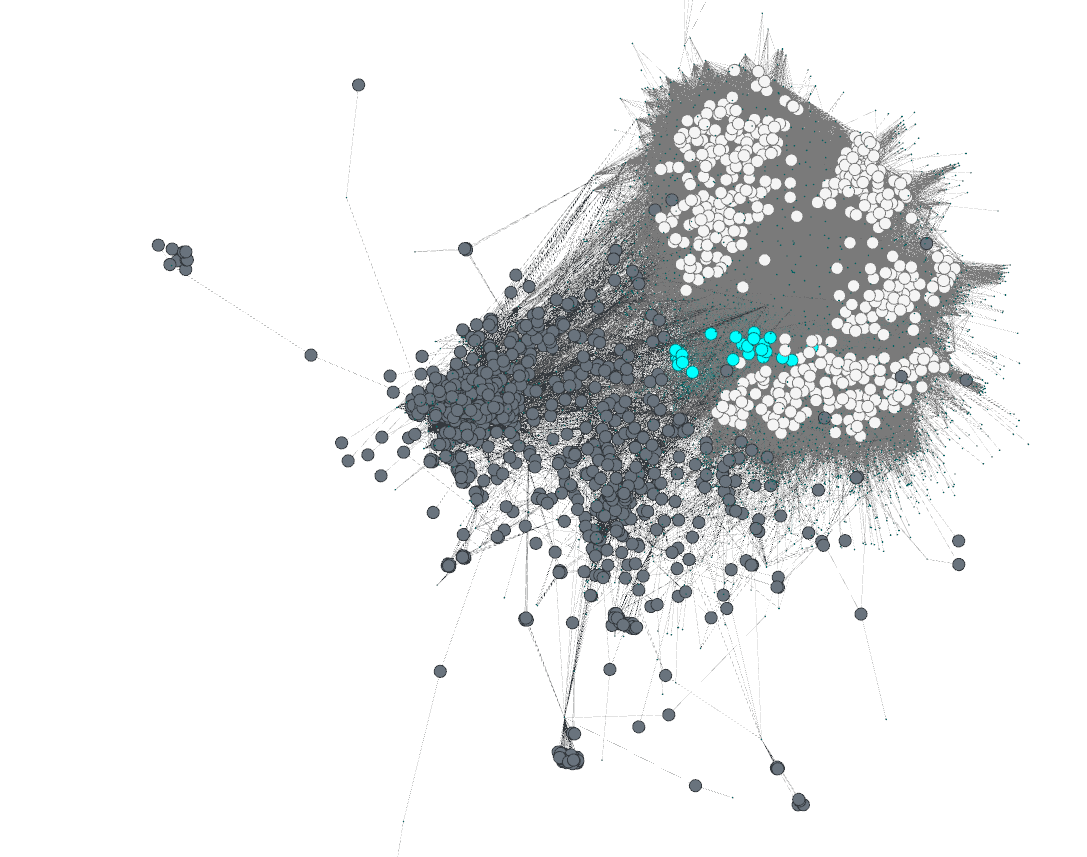
\includegraphics[width=\textwidth]{./img/gamma.png}
\subcaption{Gammaprotéobactéries}\label{figgamma}
\end{minipage}
\caption[Visualisation par graphe des réplicons par lignée bactérienne]{Visualisation par graphe bipartite des réplicons $V^{R_{taxon}}$ selon la taxonomie de leur hôte (phylum ou classe pour les Protéobactéries).\\\medskip Coloration selon le type de réplicon : chromosome (gris clair), plasmide (gris foncé), RECE (bleu). Les clusters de protéines (vert foncé) sont visibles pour certaines résolutions.} \label{figgprahe2}
\end{center}
\end{figure}
\end{landscape}


\begin{figure}[H]
\hspace{-2cm}
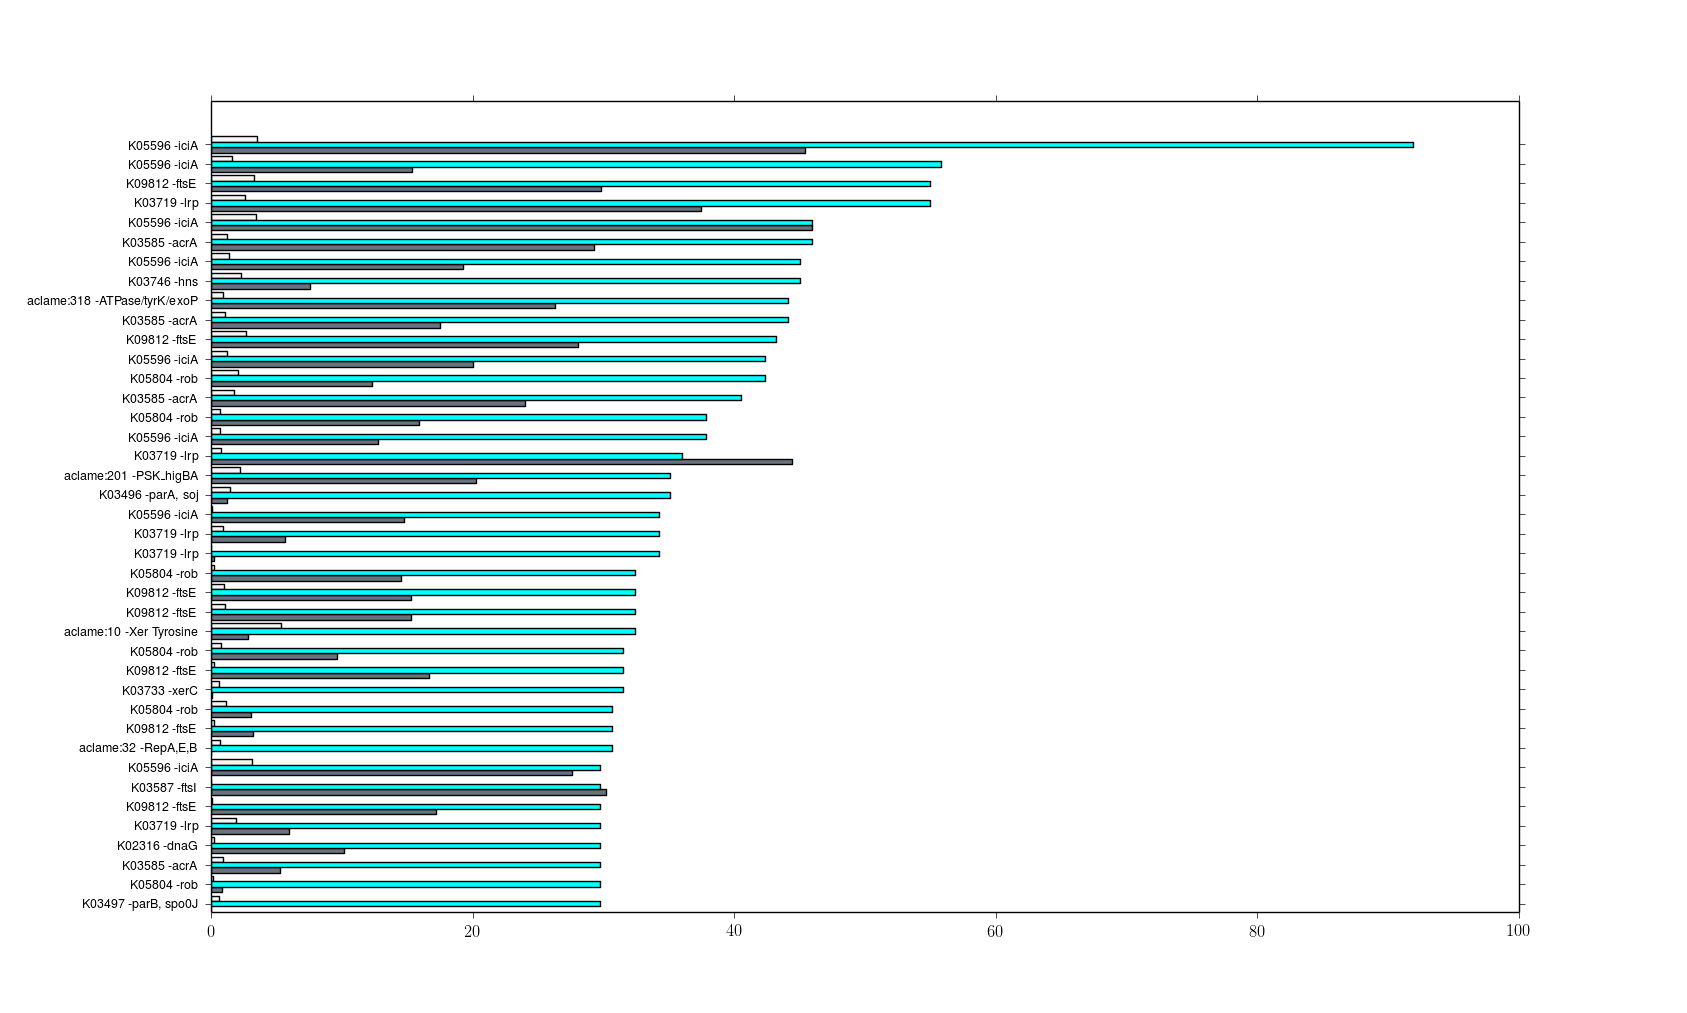
\includegraphics[trim=0cm 1cm 0cm 0cm,clip,width=1.2\textwidth, height=0.7\textheight]{./img/cluster_connectivity2.png}
%\mbox{\footnotesize\hspace{4cm} Pourcentages d'observations connectées aux clusters (par type)}
\caption[Pourcentages de connexion aux clusters de protéines par type de réplicon]{Pourcentages, par type de réplicon, de connexion aux 40 clusters de protéines les plus connectés aux observations annotées en tant que RECE de $\bar{V}^{R_{\textrm{Protéobactéries}}}_{genre}$. Pour chaque cluster (ordonnée), sont représentés les pourcentages de connexion (abcisse) pour les observations annotées en tant que RECE (bleu), chromosome (gris foncé) et plasmide (gris clair).}\label{figconnectiv}
\end{figure} 

   Dans l'interprétation visuelle des graphes obtenus par ForceAtlas2, un des biais vient du positionnement de certains plasmides faiblement connectés dans certains groupes de chromosomes hautement connectés s'ils sont liés à des clusters de protéines communs. Il est de plus difficile de comparer la pertinence visuelle des graphes bipartites spatialisés avec les visualisations obtenues par projection. 

\subsubsection{Logiciels utilisés}
 \begin{description}
 \item[Gephi] \citep{Bastian2009} logiciel ``open source" de graphes, a été utilisé pour spatialiser (en utilisant ForceAtlas 2) et visualiser les graphes.
 \item[Python] a été utilisé pour réaliser les nombreux workflows, préparer les données, préparer les fichiers \textit{graphml} utilisés par Gephi. 
 \end{description}
 
 
 
\subsection{Visualisation: discussion}

  La projection des réplicons selon leurs STIG par MDS et SOM et la visualisation par graphe montrent que \textbf{\color{orange}les réplicons s'organisent par groupe taxonomique et selon leur type}. Même si les chromosomes et plasmides forment des groupes et communautés distinctes, ils partagent tout de même de nombreux gènes des STIG, témoignant de phénomènes d'échange génétique inter-réplicons dans les génomes bactériens. Les RECE semblent de plus posséder une distribution des gènes des STIG les distinguant des chromosomes et plasmides, et se positionnent à l'interface entre chromosomes et plasmides. Il existe différents degrés d'interconnection des RECE avec les chromosomes et les plasmides selon les RECE. \textbf{Cependant, compte tenu de la grande complexité des données, ces premiers résultats ne permettent pas d'identifier avec certitude des caractéristiques spécifiques des RECE. }
  
  
  
\section{Classification non-supervisée}\label{parclassifnonsupervis}
      L'analyse de clustering des réplicons bactériens a pour objectif principal d'étudier le comportement des RECE par rapport aux autres réplicons. Le positionnement de manière stable d'un RECE dans un groupe de chromosomes ou un groupe de plasmides indiquerait une proximité avec les membres de ce groupe. À l'inverse un cluster homogène de RECE peut être le témoin de leur spécificité et les différencier en tant qu'espèce moléculaire distincte des autres réplicons. 
      
 \subsection{Algorithmes de clustering}\label{paralgoclust}
      
      Différents algorithmes de clustering ont été testés, les critères retenus étant le temps d'exécution, l'implémentation ou l'implémentabilité, les performances mesurées et la stabilité. Pour prendre en compte la très haute dimensionalité des données, différentes approches ont été suivies:
      
      \begin{description}
       \item[i)] Algorithmes de clustering spécifiques pour des données en grandes dimensions 
       \item[ii)] Réduction de dimension initiale par projection des données puis clustering dans ce nouvel espace
	  \item[iii)] Clustering des graphes bipartites de $V^{R}$ et $\bar{V}^{R}_{genre}$.
       \end{description}

        Les méthodes de réduction de dimensions testées sont les mêmes que précédemment (Table \ref{tabprojec}) avec $q$, le nombre de dimensions, variable. Soient $Cl$ un clustering de $C$ clusters, $V$ un ensemble d'observations et $d$ une distance. La Table \ref{tabalgoclust} introduit brièvement les principaux algorithmes de clustering utilisés
.

\begin{longtable}{ @{\hspace{-2cm}} >{\bfseries}p{0.15\textwidth}@{\hspace{1cm}}|>{\small}p{\textwidth}}
      \caption[Algorithmes de clustering utilisés]{Principaux algorithmes de clustering utilisés dans l'analyse des données.}\\ \label{tabalgoclust}
      K-Means & \citep{hartigan1975clustering,hartigan1979algorithm} Algorithme de clustering des plus populaires. Le principe original consiste à minimiser l'erreur $E=\sum_{C \in Cl}\sum_{r \in C} d(v_{r},\bar{v}^{C})$. Les paramètres de l'algorithme étant la distance $d$, le nombre de clusters $k$, le nombre d'itérations et d'exécutions de l'algorithme et son mode de convergence. De nombreuses variantes de l'algorithme existent \citep{gan2007data}.
	\\[0.4cm]
     Classifieurs \mbox{Hiérarchiques} \mbox{Agglomératifs} (CHA)
      & Algorithmes partant d'un état initial où chaque observation est considérée comme une feuille (ou nœud terminal) d'un arbre, puis formant des clusters d'observations en fusionnant de façon itérative les feuilles de cet arbre \citep{gan2007data}. Différents critères peuvent être utilisés pour choisir la fusion optimale entre deux nœuds, comme par exemple la distance minimale, maximale ou moyenne entre les observations de deux nœuds, la distance entre les centroïdes des nœuds, ou la méthode WARD (\textit{cf.} ci-dessous). 
	\\[0.4cm]
     WARD & \citep{ward1963hierarchical,ward1963application} Algorithme de la famille des classifieurs hiérarchiques agglomératifs. À partir d'un ensemble de clusters intermédiaires, le principe de cette famille d'algorithmes est de fusionner deux clusters si et seulement si un certain critère objectif est minimal \citep{gan2007data}. La méthode de Ward consiste à regrouper deux clusters intermédiaires d'un clustering $Cl_{i}$ de façon à ce que l'inertie intra-cluster $I=\frac{1}{|Cl_{i}|}\sum_{C \in Cl}\sum_{r \in C}d^{2}(v_{r},\bar{v}^{C}) $ soit minimisée.
	\\[0.4cm]
     DBSCAN & \citep{ester1996density} Algorithme de clustering par densité. D'une manière itérative, une observation $r$ est ajoutée à un cluster existant $C$ si ceux-ci sont joignables par densité selon $d$, c'est-à-dire s'il existe une observation $r_{i} \in C$ telle que $d(v_{r},v_{r_{i}})\leqslant v_{seuil}$. Les paramètres de l'algorithme étant $d$, $v_{seuil}$ et le nombre de points minimum d'un cluster. Cet algorithme s'applique cependant difficilement aux données de dimensionalité élevée car elles sont alors éparpillées dans l'espace de représentation \citep{gan2007data} (voir aussi \ref{parfleau}).
	\\[0.4cm]
     SUBCLU & \citep{Vista2004} Algorithme de clustering des données de dimensionalité élevée. Le principe est d'exécuter une procédure DBSCAN dans les différents sous-espaces où les données sont joignables par densité. Les différents sous-espaces sont sélectionnés de façon similaire à l'algorithme \textit{a priori} \citep{agrawal1994fast}. Les paramètres de SUBCLU sont les mêmes que ceux de DBSCAN.
	\\[0.4cm]
     INFOMAP & \citep{rosvall2008maps} Algorithme de détection de communautés d'un graphe $G$. Les données étant transformées en graphe bipartite par la relation \ref{eqbipartite}. Dans l'algorithme INFOMAP, une communauté est définie de façon assez similaire à celles de l'algorithme MCL: un trajet aléatoire dans un graphe aura plus tendance à rester au sein d'une communauté que d'en sortir, chaque étape du trajet étant décrit par une séquencesd'étapes représentant les différents nœuds déjà traversés et par différentes probabilités d'occurence de la prochaine étape. INFOMAP semble de plus être un des algorithmes les plus précis quand à la découverte de communautés au sein d'un graphe \citep{lancichinetti2009community}, les paramètres de l'algorithme étant le nombre de trajets aléatoires. Il est intéressant de constater qu'en utilisant un graphe bipartite comme structure, les observations ainsi que les variables sont \textit{clusterisées}.
\end{longtable}
    
La stratégie finalement retenue a été: i) d'utiliser une procédure de réduction de dimensions par ACP sur $V^{R}$ et $\bar{V}^{R}_{genre}$ puis un clustering des données projetées par l'algorithme de WARD, ii) d'exprimer $V^{R}$ et $\bar{V}^{R}_{genre}$ sous forme de graphes bipartites par l'éq. \ref{eqbipartite} puis d'utiliser l'algorithme INFOMAP. Ces deux procédures donnent les meilleurs résultats en terme de performance et présentent les meilleurs compromis en terme de temps d'exécution et d'implémentation. \\
En effet, l'algorithme du K-Means nécessite de nombreux \textit{runs} pour présenter des résultats performants et, d'un point de vue pratique, est plus lent que WARD. Par ailleurs, une méthode de classification hiérarchique comme WARD peut mieux correspondre à l'organisation taxonomique sous-jacente des données. 
Additionnellement, une procédure de CHA est effectuée en utilisant la distance \textit{cosine}, choix motivé par l'obtention de projections pertinentes par MDS en utilisant cette distance. Les résultats obtenus témoignent d'une structuration des plasmides selon la taxonomie mais se révèlent incapable de structurer les chromosomes (Table \ref{tabresvmstab}). 
L'approche de SUBCLU, bien qu'intéressante, était infaisable en pratique car elle requiert un nombre considérable de procédures DBSCAN pour les données utilisées et donc un temps de calcul (de l'ordre de la semaine) qu'il n'était pas possible d'envisager.
De par la nature des données, une représentation en graphe bipartite semblait être une approche judicieuse: l'interconnection des réplicons \textit{via} les clusters protéiques est un critère plus intuitif que la mesure d'une distance inter-réplicons. En comparaison avec d'autres algorithmes de détection de communautés (MCL, WalkTrap, Edges Betweenness, Méthode de Newman, Multilevel) \citep{Coscia2011}, INFOMAP semble produire de meilleurs résultats (résultats non montrés).
La projection par ACP a été favorisée pour sa rapidité, sa popularité, l'absence de paramètres nécessaires et sa capacité à décorréler les variables \citep{duby2006analyse}. L'utilisation de MDS et de la distance \textit{cosine} produit, avec WARD, des clusters pour lesquels une structuration des réplicons d'un point de vue taxonomique et selon leurs types est retrouvée, mais avec des scores de stabilité très bas ($\bigtriangleup^{Kl}<0.5$) rendant les clusters non interprétables en pratique.
Bien qu'INFOMAP semble présenter des sérieux avantages, la procédure ACP+WARD a été conservée pour deux raisons: i) elle présente des résultats performants en particulier pour la classification de réplicons qui sont liés à de nombreux clusters de protéines. ii) L'organisation des réplicons est fondée sur des critères de distance entre réplicons. Il est alors important de confronter les résultats de ACP+WARD avec ceux obtenus avec INFOMAP. \\
 L'objectif de cette approche est d'estimer l'organisation générale des réplicons selon leurs distributions en protéines similaires, liées aux STIG. D'un point de vue méthodologique, différentes approches complémentaires auraient pu être des choix judicieux:
 
\begin{description} 
\item[\textbullet] Tester les algorithmes de clustering dans des sous-espaces \citep{gan2007data}, de type SUBCLU, comme par exemple CLIQUE, MAFIA, PROCLUS \citep{gan2007data,han2012data}
\item[\textbullet] Tester des approches de discrétisation d'attributs \citep{witten2013data}
\item[\textbullet] Faire une étude comparative plus exhaustive sur les méthodes de projection couplées à des algorihmes de clustering classiques
\item[\textbullet] Tester des approches expérimentales et/ou novatrices de détection de communautés 
\end{description}

\begin{table}
\caption[Évaluation des procédures de clustering de $V^{R}$ et $\bar{V}_{genre}^{R}$]{Évaluation des procédures de clustering de $V^{R}$ et $\bar{V}_{genre}^{R}$.}\label{tabresvmstab}
\hspace{-2cm}
%\begin{center}
	  \begin{tabular}{l|l|cc|cc|cc}
        & \textbf{Indice$^{a}$} & \multicolumn{2}{l|}{\textbf{ACP+WARD}} & \multicolumn{2}{l|}{\textbf{INFOMAP}} & \multicolumn{2}{|c}{\textbf{CHA}} \\
      \hline
      &&&&&&\\[-0.2cm]
      Données & & $V^{R}$  & $\bar{V}^{R}_{genre}$  & $V^{R}$  & $\bar{V}^{R}_{genre}$ & $V^{R}$  & $\bar{V}^{R}_{genre}$  \\
      \multirow{2}{*}{Paramètres$^{b}$} & & k: 200  &  k: 100 & \multicolumn{2}{l|}{itération: 500}& k: 200  &  k: 100  \\
      & & cp: 30 & cp: 15 & & \\
      Nombre de clusters$^{c}$ &  &175 & 75 & 223 & 77 & 174 & 67\\
      Variance expliquée (ACP) & & 0.57\% & 0.58\% & & \\
      \hline
      &&&&&&\\[-0.2cm]
     \textbf{Critère de stabilité$^{d}$:} $\bigtriangleup^{Kl}$ & & 0.85 & 0.74 & 0.82 & 0.76 & 0.79 & 0.70 \\
      \hline
      \multirow{3}{*}{\textbf{Type de réplicons}} & \textit{homogeneity} &0.93 & 0.83 & 0.80 & 0.63 & 0.90 & 0.83 \\
       & \textit{completeness} & 0.25 & 0.20 & 0.15 & 0.15 & 0.18 & 0.21\\
       & \textit{V-measure} & 0.43 & 0.32 & 0.25 & 0.24 & 0.31 & 0.34\\
      \hline
      \multirow{3}{*}{\textbf{Phylum des chromosomes}} & \textit{homogeneity} & 0.93 & 0.80 & 0.93 & 0.69 & 0.62 & 0.59 \\
       &\textit{completeness} & 0.35 & 0.40 & 0.60 & 0.61 & 0.65 & 0.65\\
       &\textit{V-measure} & 0.51 & 0.53 & 0.73 & 0.65 & 0.64 & 0.62\\
      \hline
      \multirow{3}{*}{\textbf{Classes des chromosomes}} & \textit{homogeneity} & 0.93 & 0.80 & 0.85 & 0.64 & 0.60 & 0.55 \\
       &\textit{completeness} & 0.16 & 0.58 & 0.80 & 0.82 & 0.93 & 0.89\\
       &\textit{V-measure} & 0.66 & 0.67 & 0.82 & 0.72 & 0.73 & 0.68\\
      \hline
      \multirow{3}{*}{\textbf{Phylum des plasmides}} & \textit{homogeneity} & 0.06 & 0.01 & 0.88 & 0.78 & 0.85 & 0.68 \\
       &\textit{completeness} & 0.16 & 0.14 & 0.33 & 0.35 & 0.30 & 0.32\\
       &\textit{V-measure} & 0.08 & 0.02 & 0.48 & 0.48 & 0.45 & 0.43\\
      \hline
      \multirow{3}{*}{\textbf{Classes des plasmides}} & \textit{homogeneity} & 0.07 & 0.02 & 0.84 & 0.74 & 0.81 & 0.68 \\
       &\textit{completeness} & 0.28 & 0.36 & 0.43 & 0.51& 0.41& 0.49\\
       &\textit{V-measure} & 0.12 & 0.03 & 0.57 & 0.60 & 0.54 & 0.57\\
      \hline
      \end{tabular}
      \captionsetup{labelsep=space,justification=justified,singlelinecheck=off}
      \vspace{0.5cm}
\caption*{$^{a}$ \textit{V-measure} calculées selon l'éq. \ref{eqvm}. \\ $^{b}$ $k$, nombre de clusters en \textit{input} et  $cp$, nombre de composantes principales retenues pour la classification par WARD. \\ $^{c}$ Nombre de clusters obtenus par les algorithmes.\\ $^{d}$ Critère de stabilité $\bigtriangleup^{Kl}$ calculé par l'éq. \ref{eqestimstaball}}
\captionsetup{}
%\end{center}
\end{table}

\subsubsection{Logiciels utilisés}
 \begin{description}
 \item[Scikit-learn] librairie de Machine learning de Python utilisée pour le calcul des projections par ACP, MDS, pour les procédures de clustering par les algorithmes DBSCAN, CHA, et WARD, ainsi que pour le calcul des indices de V-measure (\textit{homogeneity}, \textit{completeness}).
 \item[Pycluster] \citep{de2004open}  utilisé pour les procédures de clustering par K-Means, notamment.
 \item[igraph] \citep{csardi2006igraph} a été utilisé \textit{via} Python pour l'utilisation des algorithmes de détection de communautés: INFOMAP notamment.
 \item[Python]  utilisé pour réaliser les workflows, préparer les données, calculer les distances inter-observations, ainsi que pour réaliser une implémentation de l'algorithme SUBCLU.
 \item[C++] a été utilisé en parallèle avec Python pour coder certaines parties de divers algorithmes. 
 \end{description}

      \subsection{Résultats du clustering}\label{parresultatclustering}
      
	  Les résultats de l'étude de stabilité et de la séparation des différents ensembles étudiés sont présentés Table \ref{tabresvmstab}. L'organisation et les spécificités des différents clusters contenant des RECE sont de plus présentées Table \ref{tabrececluster}. Pour la procédure ACP+WARD, différentes valeurs de $k$ et de nombre de composantes principales $cp$ ont été testées. $cp$ a été choisi en fonction de l'évolution de la variance expliquée par les composantes et de la stabilité des clusters obtenus et $k$ a été choisi en fonction des indices de stabilité. De même, le choix de $k$ pour la procédure CHA s'est effectué \textit{via} les scores de stabilité.\\
	   Les trois méthodes produisent des clusters stables et exploitables dans leur ensemble. Ces procédures parviennent à séparer clairement les plasmides des chromosomes, comme attendu. Cependant, seul ACP+WARD et INFOMAP arrivent à séparer de façon efficace les chromosomes selon leur phylum ou classe taxonomique, ce qui indique une cohérence biologique des résultats. L’échec de CHA à structurer les chromosomes est probablement dû au fait qu'il existe des différences trop importantes de densité entre les groupes de chromosomes et de plasmides et qu'ainsi, les chromosomes sont considérés comme un groupe homogène par rapport aux clusters de plasmides et sont donc difficilement divisés par l'algorithme. Il est intéressant de constater qu'INFOMAP arrive à identifier des clusters ayant une correspondance assez forte avec des groupes taxonomiques (indice de \textit{completeness} élevé). L'ensemble des clusters de réplicons obtenus par $f_{INFOMAP}(V^{R})$ sont présentés en Appendice \ref{AppendixD}.\\ L'utilisation de données normées selon le genre taxonomique et le type des réplicons $\bar{V}^{R}_{genre}$  tend à produire des clusters moins stables et à faire baisser les valeurs des indices d'\textit{homogeneity}. Cependant les résultats pour $V^{R}$ et $\bar{V}^{R}_{genre}$ sont globalement similaires.\\
	  La procédure ACP+WARD a tendance à grouper les plasmides au sein de clusters larges et stables, ce qui s'explique par le fait que la distance calculée $d(v_{r_{1}},v_{r_{2}})$ entre deux plasmides $r_{1}$ et $r_{2}$ par WARD est davantage sensible au phénomène du \textit{fléau de la dimensionalité} (\S \ref{parfleau}) que dans le cas des chromosomes en général. À l'inverse, INFOMAP et CHA sont capables de détecter des groupes de plasmides fortement liés à un faible nombre de clusters de protéines communs et corrélés à la taxonomie (Table \ref{tabresvmstab}). Un des bruits rencontrés dans les clusters d'INFOMAP est qu'un plasmide ou groupe de plasmides isolé(s) peut être intégré à l'intérieur de communautés de chromosomes s'ils sont fortement reliés à des clusters de protéines caractéristiques de ces communautés (ce qui explique les meilleurs scores de ACP+WARD pour la séparation des réplicons). Tout dépend alors de ce qui est considéré comme distance pertinente dans la comparaison des réplicons.
 
Le principal résultat de cette analyse est cependant la structuration des RECE dans les clusters (Table \ref{tabrececluster}). Dans l'ensemble, {\color{orange}\bf les RECE se distinguent nettement des autres réplicons en présentant des caractéristiques singulières}, ce qui produit des  clusters spécifiques de RECE. Ceci est très net chez \textit{Vibrio, Leptospira, Brucella} ou pour les Burkhoderiales (avec CHA) par exemple. Les RECE de \textit{Vibrio/Aliivibrio}  sont présents dans un unique cluster. Enfin, ceux de \textit{Sinorhizobium} sont associés avec des plasmides d'espèces de Rhizobiales. Pour les RECE des Burkholderiales et d'\textit{Agrobacterium}, les clusters obtenus contenant ces RECE sont instables et les scores individuels $\bigtriangleup^{e}$ sont faibles, rendant les résultats peu interprétables. Des clusters des RECE des Burkholderiales stables et homogènes peuvent être cependant obtenus en utilisant uniquement $V^{R_{\textrm{Betaproteobactéries}}}$, témoignant de la spécificité de ces RECE. Certains mégaplasmides des Burkholderiales appartiennent cependant à ces mêmes clusters. Les RECE II des Burkholderiales, plus interconnectés aux plasmides, ont plus tendance à être dans des clusters avec d'autres plasmides. Ces éléments sont en faveur d'une transition mégaplasmide $\Rightarrow$ RECE de type RECE II $\Rightarrow$ RECE I chez les Burkholderiales.\\
 INFOMAP tend à grouper une majorité de RECE dans des communautés de chromosomes, indiquant que chromosomes et RECE possèdent des caractéristiques communes. À l'inverse, ACP+WARD et CHA ont plus tendance à placer les RECE dans des clusters de plasmides, témoignant d'une différence significative, dans l'ensemble, entre le nombre de clusters de protéines liés aux RECE et aux chromosomes. {\color{orange}\bf Cependant on constate que certains RECE sont plus proches des chromosomes alors que d'autres sont liés de manière forte à des plasmides}.  Pour les trois méthodes, les RECE de \textit{Anabaena, Asticaccaulis, Paracoccus} et \textit{Prevotella} sont groupés de manière stable avec les chromosomes (Table \ref{tabrececluster}). Cette structuration indique clairement que ces RECE possèdent des caractéristiques propres les distinguant des plasmides. À l'inverse, certains RECE, \textit{i.e.}, chez \textit{Deinococcus, Rhodobacter, Leptospira} et \textit{Butyrivibrio}, sont classés de manière stable avec les plasmides indiquant le partage de caractéristiques communes. Enfin, un autre résultat intéressant est l'organisation (inattendue) par INFOMAP et par CHA des plasmides selon leur groupe taxonomique révélant un lien entre organisation des  STIG plasmidiques et taxonomie des bactéries les hébergeant. Pour un niveau taxonomique donné (phylum ou classe), les plasmides sont organisés en différents groupes (indice de \textit{completeness} faible), \textbf{\color{orange} indiquant que ces réplicons peuvent être caractérisés par une structuration taxonomique et fonctionnelle}. \\
 Les visualisations et les clusterings de $V^{R}$ et $V_{genre}^{R}$ montrent que la structuration des réplicons bactériens en fonction de leurs STIG dépend de la taxonomie et du type des réplicons. Il est de plus clair qu'une partie des RECE se distingue, par leurs STIG, nettement des chromosomes et des plasmides. L'ensemble des RECE semble de plus posséder un ou plusieurs gènes liés aux STIG inhabituels pour les plasmides. 

\begin{landscape}


%Agrobacterium&3&0.55&0.27&0.38&0.35&0.88&0.4\\
%Aliivibrio&1&1.0&0.0&0.0&1.0&0.95&0.95\\
%\rowcolor{Cchr}Anabaena **&1&0.96&0.96&0.02&0.02&1.0&0.9\\
%\rowcolor{Cchr}Asticcacaulis **&1&1.0&0.96&0.03&0.01&1.0&0.97\\
%Brucella&1&1.0&0.0&0.05&0.95&0.94&0.87\\
%Burkholderia&2&0.99&0.64&0.19&0.17&0.99&0.73\\
%\rowcolor{Cpl}Butyrivibrio *&1&1.0&0.0&0.5&0.5&1.0&0.83\\
%Chloracidobacterium&1&0.82&0.91&0.08&0.01&0.42&0.86\\
%Cupriavidus&1&0.99&0.73&0.09&0.18&0.98&0.72\\
%\rowcolor{Cpl}Cyanothece *&1&0.89&0.0&0.94&0.06&0.33&0.61\\
%\rowcolor{Cpl}Deinococcus **&1&0.74&0.0&0.96&0.04&1.0&0.61\\
%Ilyobacter&1&0.82&0.91&0.08&0.01&0.42&0.86\\
%\rowcolor{Cpl}Leptospira *&1&1.0&0.0&0.13&0.88&1.0&1.0\\
%Nocardiopsis&1&0.97&0.91&0.09&0.0&1.0&0.97\\
%Ochrobactrum&1&1.0&0.0&0.05&0.95&0.94&0.87\\
%\rowcolor{Cchr}Paracoccus **&1&1.0&0.96&0.03&0.01&1.0&0.97\\
%Photobacterium&1&1.0&0.96&0.03&0.01&0.72&0.79\\
%\rowcolor{Cchr}Prevotella ***&1&0.95&0.95&0.02&0.02&1.0&0.92\\
%Pseudoalteromonas&1&1.0&0.96&0.03&0.01&0.72&0.79\\
%Ralstonia&1&0.99&0.73&0.09&0.18&0.98&0.72\\
%\rowcolor{Cpl}Rhodobacter *&1&1.0&0.0&0.6&0.4&1.0&0.71\\
%\rowcolor{Cpl}Sinorhizobium **&2&1.0&0.0&0.87&0.13&0.98&0.87\\
%Sphaerobacter&1&1.0&0.0&0.5&0.5&1.0&1.0\\
%Sphingobium&2&0.98&0.7&0.29&0.01&0.75&0.94\\
%Thermobaculum&1&0.82&0.91&0.08&0.01&0.42&0.86\\
%Variovorax&1&0.99&0.73&0.09&0.18&0.98&0.72\\
%Vibrio&1&1.0&0.0&0.0&1.0&0.95&0.95\\
 
\definecolor{Cchr}{RGB}{255,228,181}
\definecolor{Cpl}{RGB}{220,220,250}
\thispagestyle{empty}
\begin{small}
		\begin{table}[h]
		\vspace{-1.5cm}
		 \hspace{-2cm}
	  \begin{minipage}[t]{0.45\linewidth}
	  \begin{tabular}{>{\bfseries}l|c|c|ccc|c|c}
	\textbf{Genre}&\textbf{C}&\textbf{\footnotesize BHIw}& \textbf{\footnotesize\%chr}&\textbf{\footnotesize\%pl}&\textbf{\scriptsize\%RECE}&$E(\bigtriangleup^{r}) $&$\bar{E}(\bigtriangleup^{C})$\\
	\hline
 Agrobacterium&3&0.9&67&16&17&0.45&0.55\\
Aliivibrio&1&1.0&0&0&100&0.97&0.94\\
\rowcolor{Cchr}Anabaena **&1&1.0&98&0&2&1.0&0.99\\
\rowcolor{Cchr}Asticcacaulis **&1&1.0&96&3&1&0.8&0.96\\
Brucella&1&1.0&0.0&5&95&1.0&0.84\\
Burkholderia&2&0.99&63&2&17&0.46&0.61\\
\rowcolor{Cpl}Butyrivibrio *&1&1.0&0&50&50&1.0&0.87\\
Chloracidobacterium&1&0.82&92&8&1&1.0&0.95\\
Cupriavidus&1&0.99&71&11&18&0.45&0.59\\
\rowcolor{Cpl}Cyanothece *&1&0.89&0&94&6&0.5&0.64\\
\rowcolor{Cpl}Deinococcus **&1&0.71&0&96&4&1.0&0.76\\
Ilyobacter&1&0.82&0.92&8&1&1.0&0.95\\
\rowcolor{Cpl}Leptospira *&1&1.0&0&13&88&1.0&0.94\\
Nocardiopsis&1&0.97&90&9&0&1.0&0.96\\
Ochrobactrum&1&1.0&0&5&95&1.0&0.84\\
\rowcolor{Cchr}Paracoccus **&1&1.0&96&3&1&0.8&0.96\\
Photobacterium&1&0.99&0.71&11&18&0.45&0.59\\
\rowcolor{Cchr}Prevotella ***&1&0.95&95&2&2&1.0&0.96\\
Pseudoalteromonas&1&0.99&97&3&1&0.98&0.82\\
Ralstonia&1&0.99&71&11&18&0.45&0.59\\
\rowcolor{Cpl}Rhodobacter *&1&1.0&0&60&40&1.0&0.9\\
\rowcolor{Cpl}Sinorhizobium **&2&0.96&0&98&2&0.67&0.65\\
Sphaerobacter&1&1.0&0.0&50&50&1.0&0.74\\
Sphingobium&2&0.95&78&20&1&0.65&0.93\\
Thermobaculum&1&0.82&92&8&1&1.0&0.95\\
Variovorax&1&0.99&71&11&18&0.45&0.59\\
Vibrio&1&1.0&0&0&100&0.97&0.94\\
	  \end{tabular}
	  \subcaption{INFOMAP}\label{subtabinfores}
	  \end{minipage}
	  \hspace{3.5cm}
	  \begin{minipage}[t]{0.45\linewidth}
	  \begin{tabular}{>{\bfseries}l|c|c|ccc|c|c}
	  \textbf{Genre}&\textbf{C}&\textbf{\footnotesize BHIw}& \textbf{\footnotesize\%chr}&\textbf{\footnotesize\%pl}&\textbf{\scriptsize\%RECE}&$E(\bigtriangleup^{r}) $&$\bar{E}(\bigtriangleup^{C}) $\\
	\hline
	Agrobacterium&2&0.94&0&71&29&0.85&0.58\\
Aliivibrio&1&1.0&0&61&39&0.95&0.66\\
\rowcolor{Cchr}Anabaena&1&0.97&98&0&2&0.0&0.84\\
\rowcolor{Cchr}Asticcacaulis **&1&1.0&88&4&8&1.0&0.88\\
Brucella &2&0.96&0&57&43&0.93&0.53\\
Burkholderia&7&0.97&0&29&71&0.8&0.68\\
\rowcolor{Cpl}Butyrivibrio *&1&0.27&0&99&1&0.96&0.98\\
Chloracidobacterium&1&0.27&0&99&1&0.96&0.98\\
Cupriavidus&1&1.0&0&25&75&0.89&0.63\\
\rowcolor{Cpl}Cyanothece *&1&0.27&0&99&1&0.96&0.98\\
\rowcolor{Cpl}Deinococcus *&1&0.27&0&99&1&0.96&0.98\\
Ilyobacter&1&0.27&0&99&1&0.96&0.98\\
\rowcolor{Cpl}Leptospira *&1&27&0&99&1&0.96&0.98\\
Nocardiopsis&1&0.58&0&98&2&0.67&0.4\\
Ochrobactrum&1&1.0&0&0&100&1.0&1.0\\
\rowcolor{Cchr}Paracoccus **&1&1.0&88&4&8&1.0&0.88\\
Photobacterium&1&1.0&0&0&100&0.51&0.54\\
\rowcolor{Cchr}Prevotella **&2&1.0&95&0&5&0.5&0.71\\
Pseudoalteromonas&2&0.28&0&98&1&0.96&0.98\\
Ralstonia&3&1.0&0&23&77&0.87&0.77\\
\rowcolor{Cpl}Rhodobacter *&2&0.65&0&94&6&0.72&0.43\\
\rowcolor{Cpl}Sinorhizobium **&2&0.94&0&79&21&0.64&0.51\\
Sphaerobacter&1&0.93&0&8&20&0.75&0.52\\
Sphingobium&1&1.0&0&61&39&0.95&0.66\\
Thermobaculum&1&0.27&0&99&1&0.96&0.98\\
Variovorax&1&1.0&0&33&67&0.5&0.48\\
Vibrio&2&1.0&0&44&56&0.74&0.63\\
	  \end{tabular}
	  \subcaption{PCA+WARD}\label{subtabpcawa}
	  \end{minipage}
	  \caption[Classification non-supervisée des RECE]{Résultats de la classification non-supervisée des RECE par INFOMAP \ref{subtabinfores} et ACP+WARD \ref{subtabpcawa} sur $V^{R}$. \\
 \textbf{C}: nombre de clusters regroupant les RECE d'un \textbf{genre} bactérien donné. \textbf{BHIw}: valeur de l'indice BHIw (éq. \ref{bhiw}) concernant le phylum de l'ensemble des réplicons de ces clusters. \textbf{\%chr}, \textbf{\%pl} et \textbf{\%RECE}: pourcentage de représentation du type des réplicons présents dans ces clusters. $E(\bigtriangleup^{r})$: valeur moyenne de l'estimateur $\bigtriangleup^{r}$ (relation \ref{eqestimstabr}) des différents RECE. $\bar{E}(\bigtriangleup^{C})$: valeur moyenne de l'estimateur $\bigtriangleup^{C}$ (relation \ref{eqestimstabC}) des différents clusters, pondérée par la taille des clusters (similaire à la relation \ref{eqestimstaball}). Surlignage : genres taxonomiques où les réplicons apparaissent clairement proches des \textbf{chromosomes} (orange) ou des \textbf{plasmides} (magenta) pour les deux procédures. Le nombre d'étoiles est un indice \underline{subjectif} de la confiance accordée à ces résultats.}\label{tabrececluster}
	  \end{table}
	  \end{small}
	 \end{landscape}
	  
	     
\newpage
\chapter{Analyse fonctionnelle des réplicons}\label{chap6true}
\lhead{\emph{Analyse fonctionnelle des réplicons}}\label{paranalysefunc}
	
	Pour caractériser les bases biologiques de la différentiation des types de réplicon, nous avons procédé à des analyses complémentaires en ne considérant plus comme variables les clusters d'homologues de protéines mais leurs annotations fonctionnelles. Chaque réplicon est ainsi décrit par une distribution de fonctions des STIG, qui sert de base à la comparaison/discrimination des réplicons. Un avantage de cette modalité de représentation est de réduire la dimensionalité des données. L'inconvénient, cependant, est que l'information liée aux homologies de séquence des protéines est perdue. Nous avons effectué trois types d'analyses fonctionnelles: i) la visualisation des réplicons et des génomes par les fonctions des clusters, ii) des analyses de régression de la distribution des fonctions selon le type de réplicon et de génome, et iii) des analyses de classification des réplicons et génomes.
	
\section{Jeux de données et notation}\label{pardonnee2}

\subsection{Notations}
Soient une protéine $p$ et son annotation $Ann(p)$ définie par la relation \ref{eqannot}, et un groupe de protéines $C$. On définit $Ann(C)$, l'annotation de $C$ par:
	 \begin{equation}
		Ann(C)=Ann(p) \iff N^{C}_{Ann(p)}=max\{N^{C}_{Ann(p_{i})}|\; p_{i} \in C\}
	\end{equation}
	où $N^{C}_{Ann(p)}$ est le nombre de fois que $Ann(p)$ apparaît dans $C$, tel que:
		 \begin{equation}
			N^{C}_{Ann(p)}=|\{Ann(p_{i})|\; p_{i} \in C \textrm{ et } Ann(p)=Ann(p_{i}) \}|
		\end{equation}

Soit un cluster de protéines $Cl$. On définit par $F$, son ensemble fonctionnel, tel que:
	\begin{equation}
		F^{Cl} = \{Ann(C)|\; C \in Cl \textrm{ et } Ann(C) \textrm{ unique} \}
	\end{equation}   

Soient $r$ un réplicon et $v_{r}$ son vecteur associé pour un clustering de protéines $Cl$ donné, défini par l'éq. \ref{eqvr}. On définit alors $v^{f}_{r}$, son vecteur fonctionnel tel que:
	\begin{equation}
		v^{f}_{r}=(N^{r}_{f_{1}},...,N^{r}_{f_{|F|}}),\; f \in F^{Cl}
	\end{equation}
où $N^{r}_{f}$ est défini par:
	\begin{equation}
		N^{r}_{f}=\sum_{\substack{{C \in Cl} \\{Ann(C)=f}}}N^{r}_{C}
	\end{equation}
avec $N^{r}_{C}$ défini par l'éq. \ref{eqvr}. \\

Pour un génome $g=\{r_{1},...,r_{|g|}\}$ (relation \ref{eqindiv}), on définit $v_{f}^{g}$ par:
	\begin{equation}
		v^{g}_{f}=(N^{g}_{f_{1}},...,N^{g}_{f_{|F|}}),\; f \in F
	\end{equation}
où $N^{g}_{f}$ est défini par:
	\begin{equation}
		N^{g}_{f}=\sum_{r \in g}N^{r}_{f}
	\end{equation}

Pour des ensembles de réplicons $R$ et de génomes $G$, on définit $V^{R}_{f}=\{v^{r}_{f}|r \in R\}$ et $V^{G}_{f}=\{v^{g}_{f}|g \in G\}$ similairement à l'éq. \ref{eqV}, ainsi que $\bar{V}^{R}_{f,n\_tax}$ similairement à l'éq. \ref{eqVnorm}. $\bar{V}^{G}_{f,n\_tax}$ est de plus défini par:
	\begin{equation}
		\bar{V}^{G}_{f,n\_tax}=\bar{V}^{Kl_{n\_tax}^{G^{\{monopartite\}}}}\cup\bar{V}^{Kl_{n\_tax}^{G^{\{multipartite\}}}}
	\end{equation}
où $G^{\{monopartite\}}$ est l'ensemble des génomes ne contenant pas de RECE et $G^{\{multipartite\}}$ est l'ensemble des génomes contenant au moins un réplicon annoté comme RECE. \\

Les annotations utilisées pour les protéines de $P_{ref}$ correspondent aux annotations de KEGG (Appendice \ref{AppendiceB}) et à nos annotations des groupes ACLAME (Appendice \ref{AppendiceC}).


\subsection{Dimension des données}
	Les 6096 clusters de protéines ($Cl$) obtenus par TRIBE-MCL avec une granularité $gr = 4$ ont été annotés par \textbf{117} fonctions (71 de KEGG et 46 de ACLAME). \textbf{2720} génomes bactériens ont de plus été formé à partir des données. Similairement aux analyses précédentes, l'indice taxonomique \textit{n\_tax} de normalisation des données choisi est le \textit{genre}. Les caractéristiques des données sont présentées Table \ref{tabdim2}.
	
\begin{table}[H]
	\caption[Dimension des données fonctionnelles]{Dimension des données.}\label{tabdim2}
	\begin{center}
	\begin{tabular}{c|c|c}
	\textbf{Ensemble de données} & \textbf{Matrice} & \textbf{Taille} \\
	\hline
	$Cl$ & - & 6096 \\
	$F^{Cl}$ & - & 117 \\
	$V^{R}_{f} $ & $M^{V^{R}_{f}}$ & (4928,117)  \\
	$\bar{V}^{R}_{f,genre} $ & $M^{\bar{V}^{R}_{f,genre}}$ & (851,117)  \\
	$V^{G}_{f} $ & $M^{V^{G}_{f}}$ & (2720,117)  \\
	$\bar{V}^{G}_{f,genre}$ & $M^{\bar{V}^{G}_{f,genre}}$ & (584,117)  \\
	\end{tabular}
	\end{center}
\end{table}	

	 
\section{Discrimination fonctionnelle des réplicons} \label{pardiscriminfuncrepl}  
	Une ségrégation fonctionnelle d'un certain groupe de réplicons est potentiellement le témoin de la spécificité fonctionnelle de ce groupe par rapport aux autres réplicons. L'objectif sous-jacent est alors d'identifier des groupes de RECE, \textbf{témoins de l'adaptation fonctionnelle de ces éléments}. La discrimination des réplicons selon leur type à partir de $V^{G}_{f}$ et $V^{R}_{f}$ a donc été recherchée. \\
	 Les composantes principales des ACP sur $V^{R}_{f}$ et $\bar{V}^{R}_{f,genre}$ permettent d'expliquer la majorité de la variance des données (Figure \ref{figpcavarianceexpl}). \\

\begin{figure}[H]
	\begin{center}
	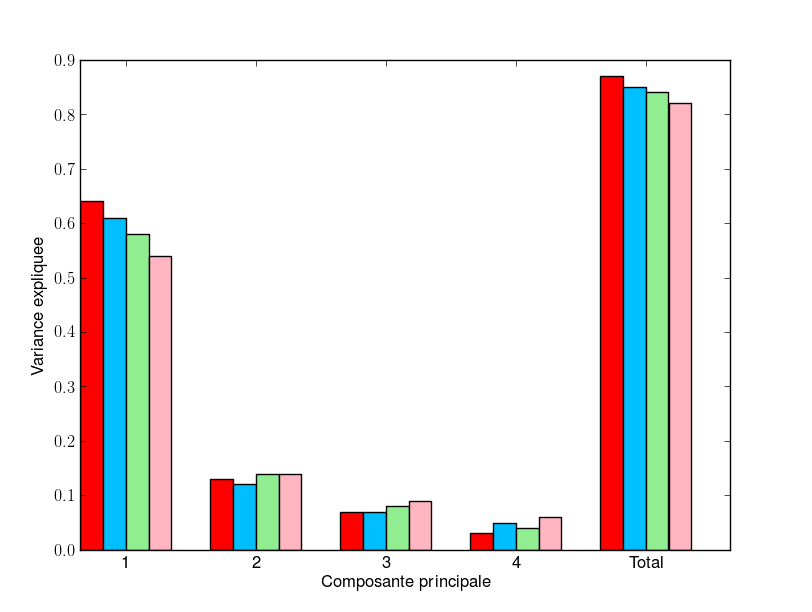
\includegraphics[scale=0.5]{./img/PCA_variance.png}
	\caption[Variance expliquée par les quatre composantes principales]{Variance expliquée par les quatre composantes principales des ACP sur $V^{R}_{f}$ (rouge), $\bar{V}^{R}_{f,genre}$ (bleu), $V^{G}_{f,genre}$ (vert) et $\bar{V}^{G}_{f,genre}$ (rose).}\label{figpcavarianceexpl}
	\end{center}	
\end{figure}	
	
	Les projections des réplicons sur les deux premières composantes sont alors utilisées pour visualiser les données. Une procédure de clustering par WARD est conduite sur les quatre premières composantes des projections de $V^{R}_{f}$ et $\bar{V}^{R}_{f,genre}$. Le choix de $k$, nombre de clusters \textit{input} de l'algorithme, est effectué en fonction du critère de stabilité $\bigtriangleup^{Kl}$ (éq. \ref{eqestimstaball}) pour $k \in \{3,10,20,50,70,100,150\}$. Les clusters obtenus sont globalement stables ($\bigtriangleup^{Kl} \thickapprox 0,75$) et sont donc interprétables (Table \ref{tabresclusterrecefunc}). 

\begin{table}[H]
	\begin{center}
	\caption[Évaluation des procédures de clustering fonctionnel des réplicons]{Évaluation des procédures de clustering de $V_{f}^{R}$ et $\bar{V}_{f,genre}^{R}$.}	\label{tabresclusterrecefunc}
	\begin{tabular}{l|c|cccc}
		 & \textbf{Indice$^{a}$}  & \multicolumn{2}{l}{\textbf{ACP+WARD}}   \\
		\hline
		 &  &  &  &   \\[-0.2cm]
		Données &  & $V_{f}^{R}$  & $\bar{V}_{f,genre}^{R}$   \\
		\multirow{2}{*}{Paramètres de WARD$^{b}$} &  & \textit{k}: 50  &  \textit{k}: 20  \\
		 &  & \textit{cp}: 4 & \textit{cp}: 4  \\
		Nombre de clusters (ACP) &  & 49 & 19  \\
		Variance expliquée (ACP) &  & 87\% & 85\%  \\
		\hline
		 &  &  &  &  \\ [-0.2cm]
		\textbf{Critère de stabilité}$^{c}$ $\bigtriangleup^{Kl}$ &  & 0.80 & 0.71  \\
		\hline
		\multirow{3}{*}{\textbf{Type de réplicon}} & \textit{homogeneity} & 0.85 & 0.68  \\
	 	& \textit{completeness} & 0.30 & 0.23 \\
		& \textit{V-measure} & 0.44 & 0.35 \\
		\hline
		\multirow{3}{*}{\textbf{Phylum des chromosomes}} & \textit{homogeneity} & 0.50 & 0.44  \\
		& \textit{completeness} & 0.27 & 0.33 \\
		& \textit{V-measure} & 0.35 & 0.38 \\
		\hline
		\multirow{3}{*}{\textbf{Classe des chromosomes}} & \textit{homogeneity} & 0.47 & 0.37  \\
		& \textit{completeness} & 0.36 & 0.41  \\
		& \textit{V-measure} & 0.41 & 0.39  \\
		\hline
		\multirow{3}{*}{\textbf{Phylum des plasmides}} & \textit{homogeneity} & 0.02 & 0.02  \\
		& \textit{completeness} & 0.10 & 0.3  \\
		& \textit{V-measure} & 0.03 & 0.03  \\
		\hline
		\multirow{3}{*}{\textbf{Classe des plasmides}} & \textit{homogeneity} & 0.03 & 0.02  \\
		& \textit{completeness} & 0.25 & 0.28  \\
		& \textit{V-measure} & 0.05 & 0.03  \\	
	\end{tabular}
	\medskip
	\captionsetup{justification=justified}
	\caption*{$^{a}$ \textit{V-measure} calculée selon l'éq. \ref{eqvm}. \\ $^{b}$ $k$, nombre de clusters en \textit{input} et $cp$ nombre de composantes principales retenues pour la classification par WARD. \\$^{c}$ Critère de stabilité $\bigtriangleup^{Kl}$ calculé par l'éq. \ref{eqestimstaball}}
	\captionsetup{}	
	\end{center}
\end{table}
		

\begin{description}
\item[\textbullet] \textbf{Chromosomes, plasmides et RECE sont discriminés fonctionnellement selon les annotations de leurs protéines des STIG.} Les chromosomes et plasmides forment deux ensembles distincts (Table \ref{tabresclusterrecefunc}; Figures \ref{figpcascatterplot} et \ref{tabrecespecificfunc}), confirmant les spécificités fonctionnelles respectives de leurs STIG. 
\end{description}
\iffalse
\begin{landscape} 
	\thispagestyle{empty}
	\begin{figure}
	\vspace{-3.5cm}
	\begin{flushleft}
	\hspace{-2cm}
	\begin{subfigure}[t]{0.42\textwidth}
	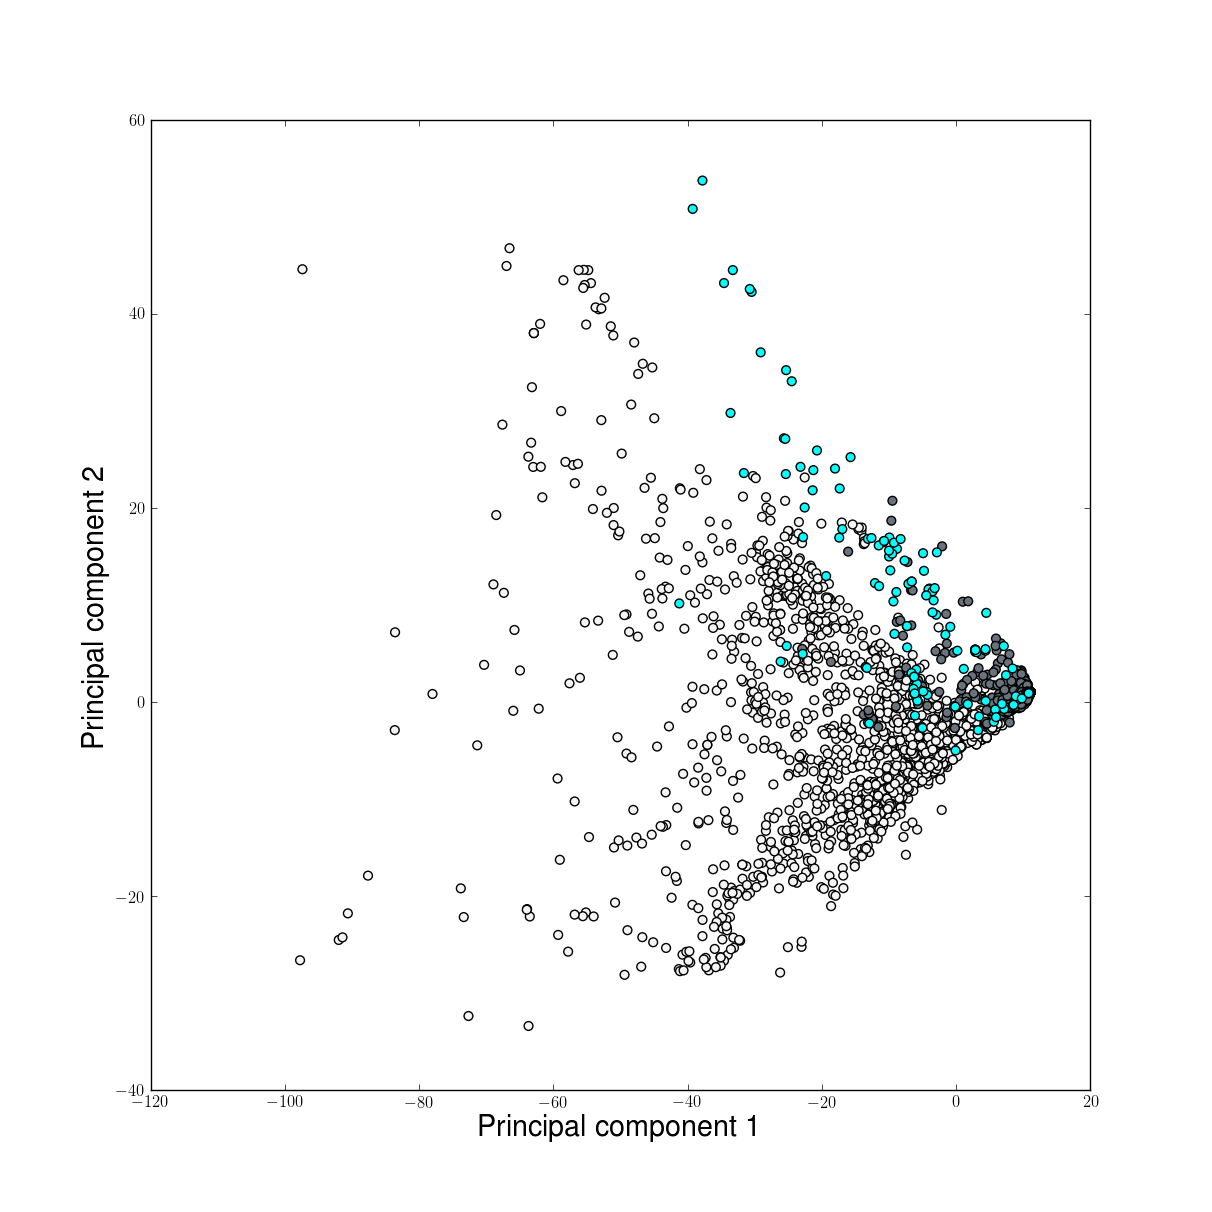
\includegraphics[width=1\textwidth]{./img/PCAcoor01.png}
	\end{subfigure}
	\begin{subfigure}[t]{0.42\textwidth}
	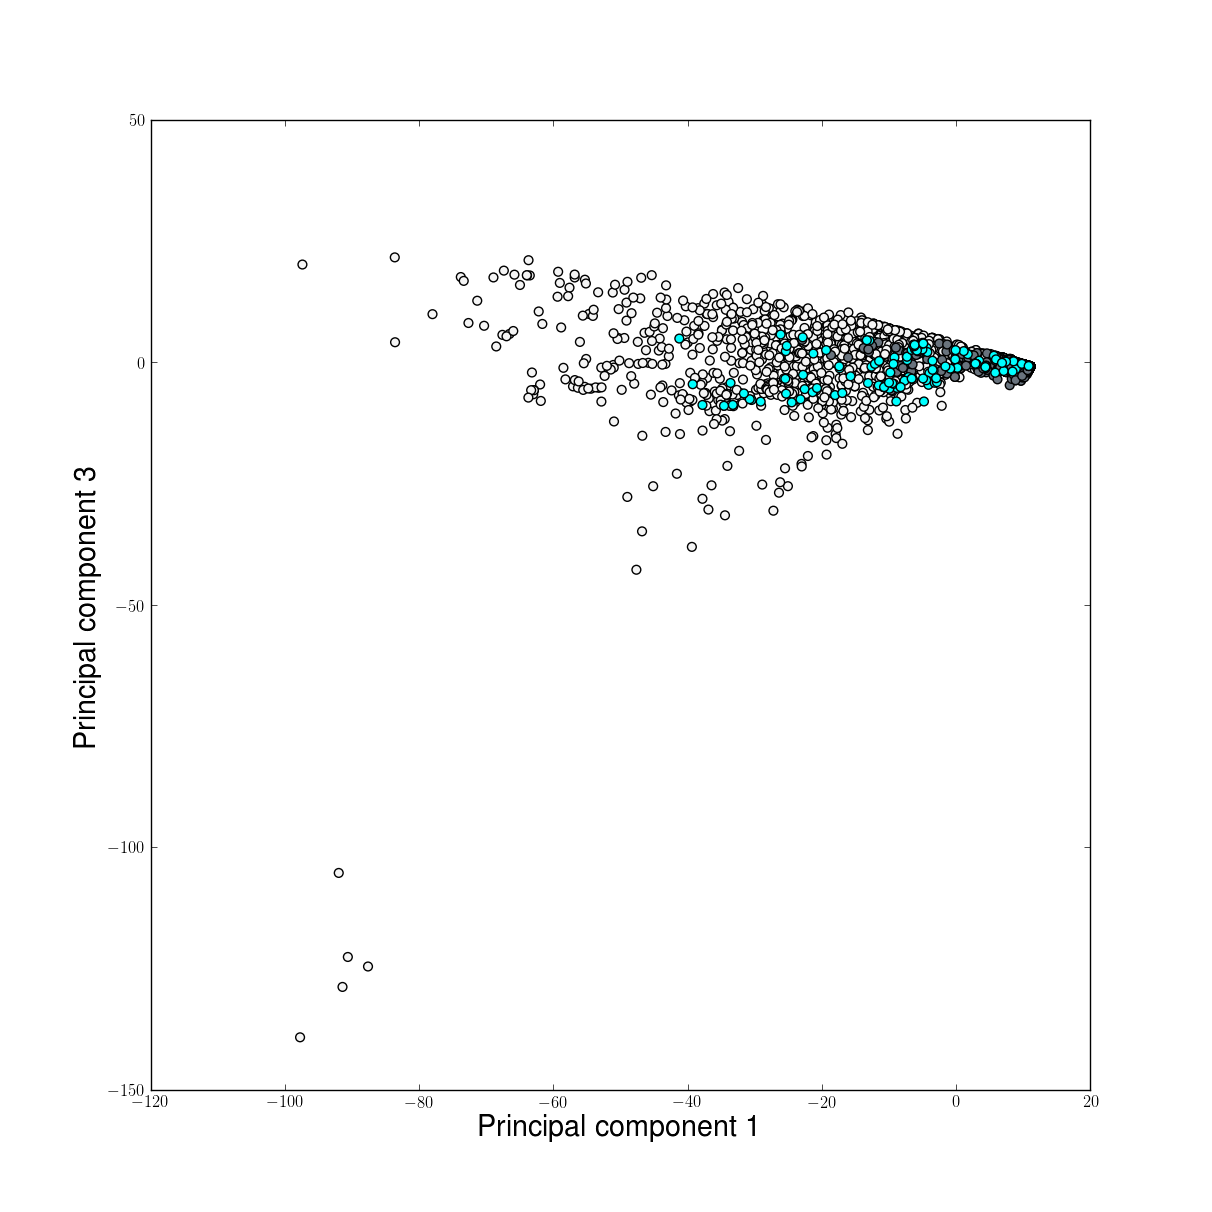
\includegraphics[width=1\textwidth]{./img/PCAcoor02.png}
	\end{subfigure}
	\begin{subfigure}[t]{0.42\textwidth}
	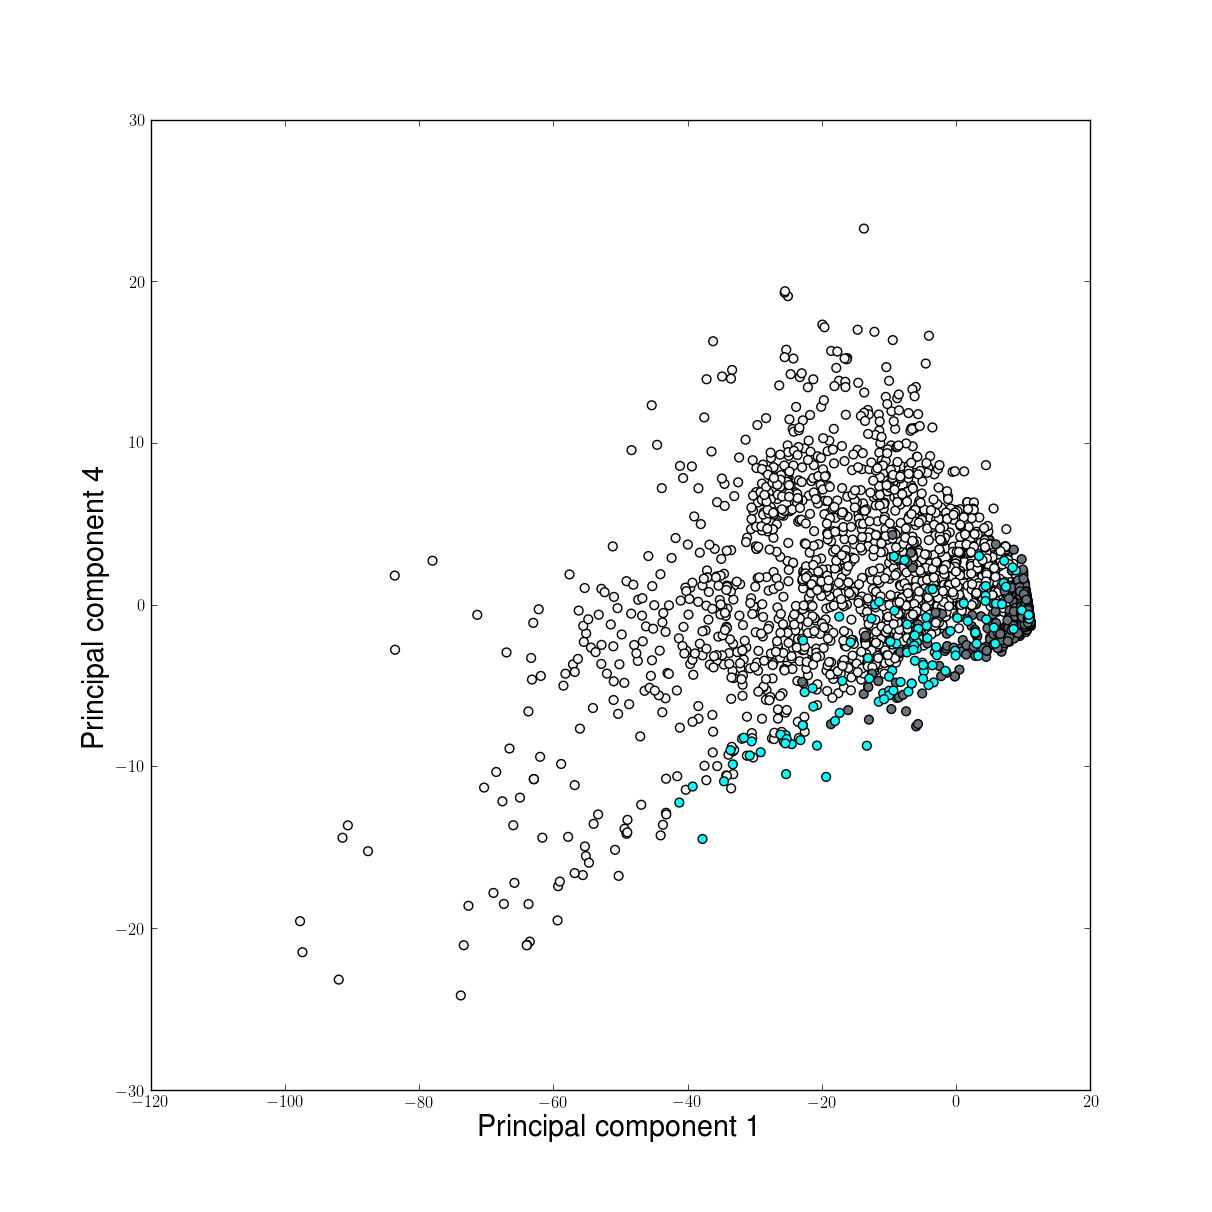
\includegraphics[width=1\textwidth]{./img/PCAcoor03.png}
	\end{subfigure}
	%\hspace{0.8cm}
	\begin{subfigure}[t]{0.42\textwidth}
	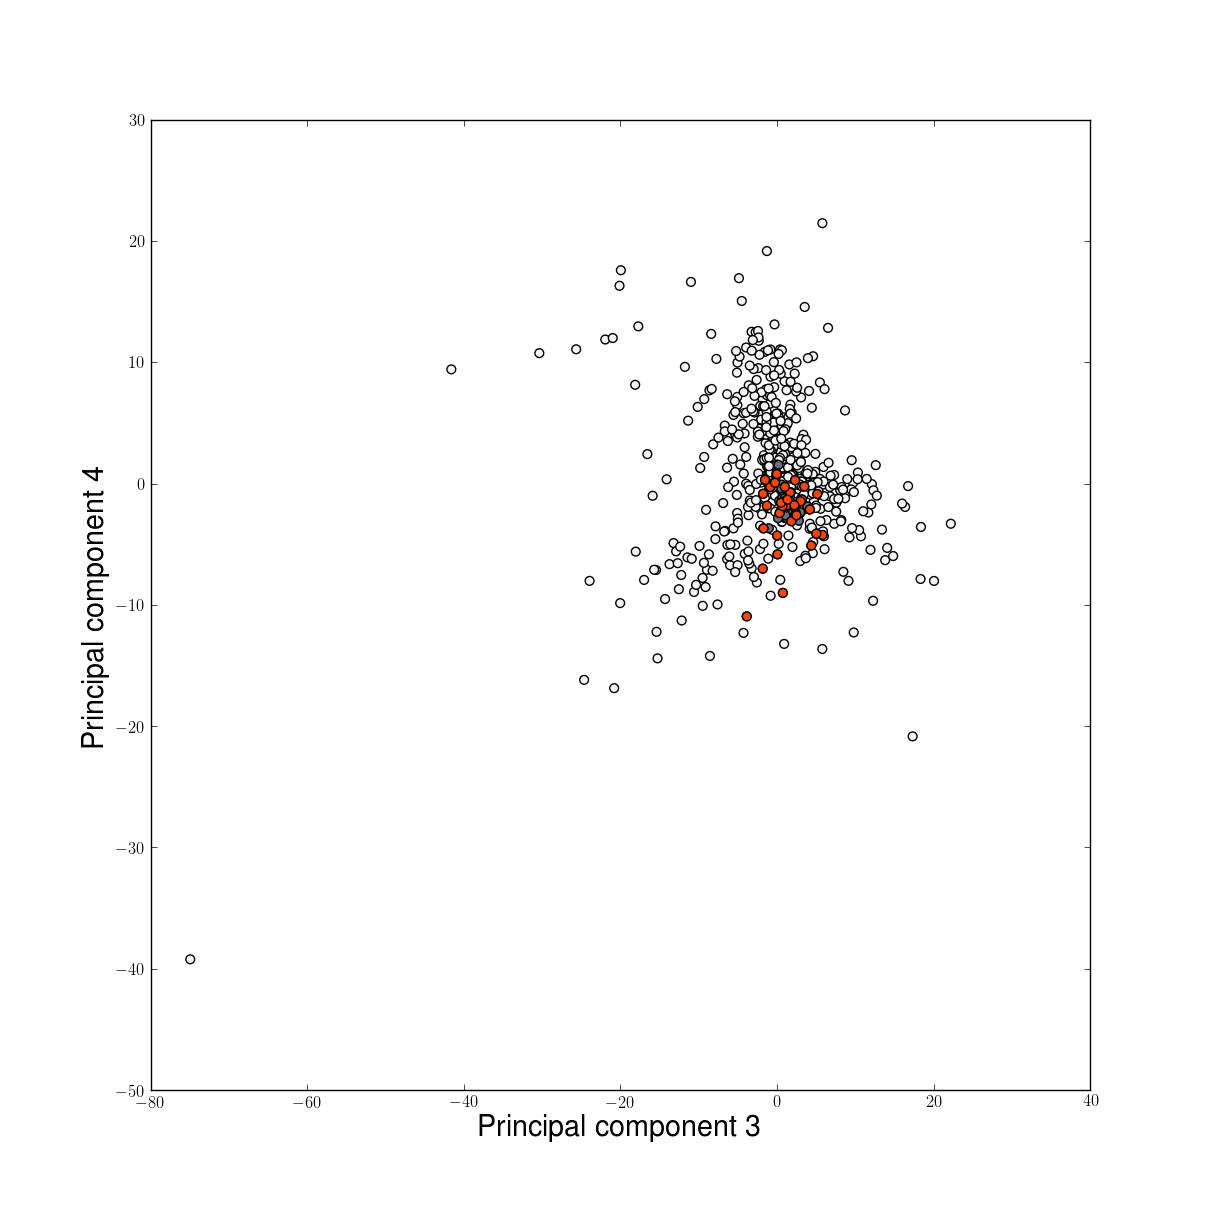
\includegraphics[width=1\textwidth]{./img/PCAncoor23.png}
	%\line(0,1){0.9\textwidth}
	\end{subfigure}
	\\
	%\vspace{-0.5cm}
	\hspace{-2cm}
	\begin{subfigure}[t]{0.42\textwidth}
	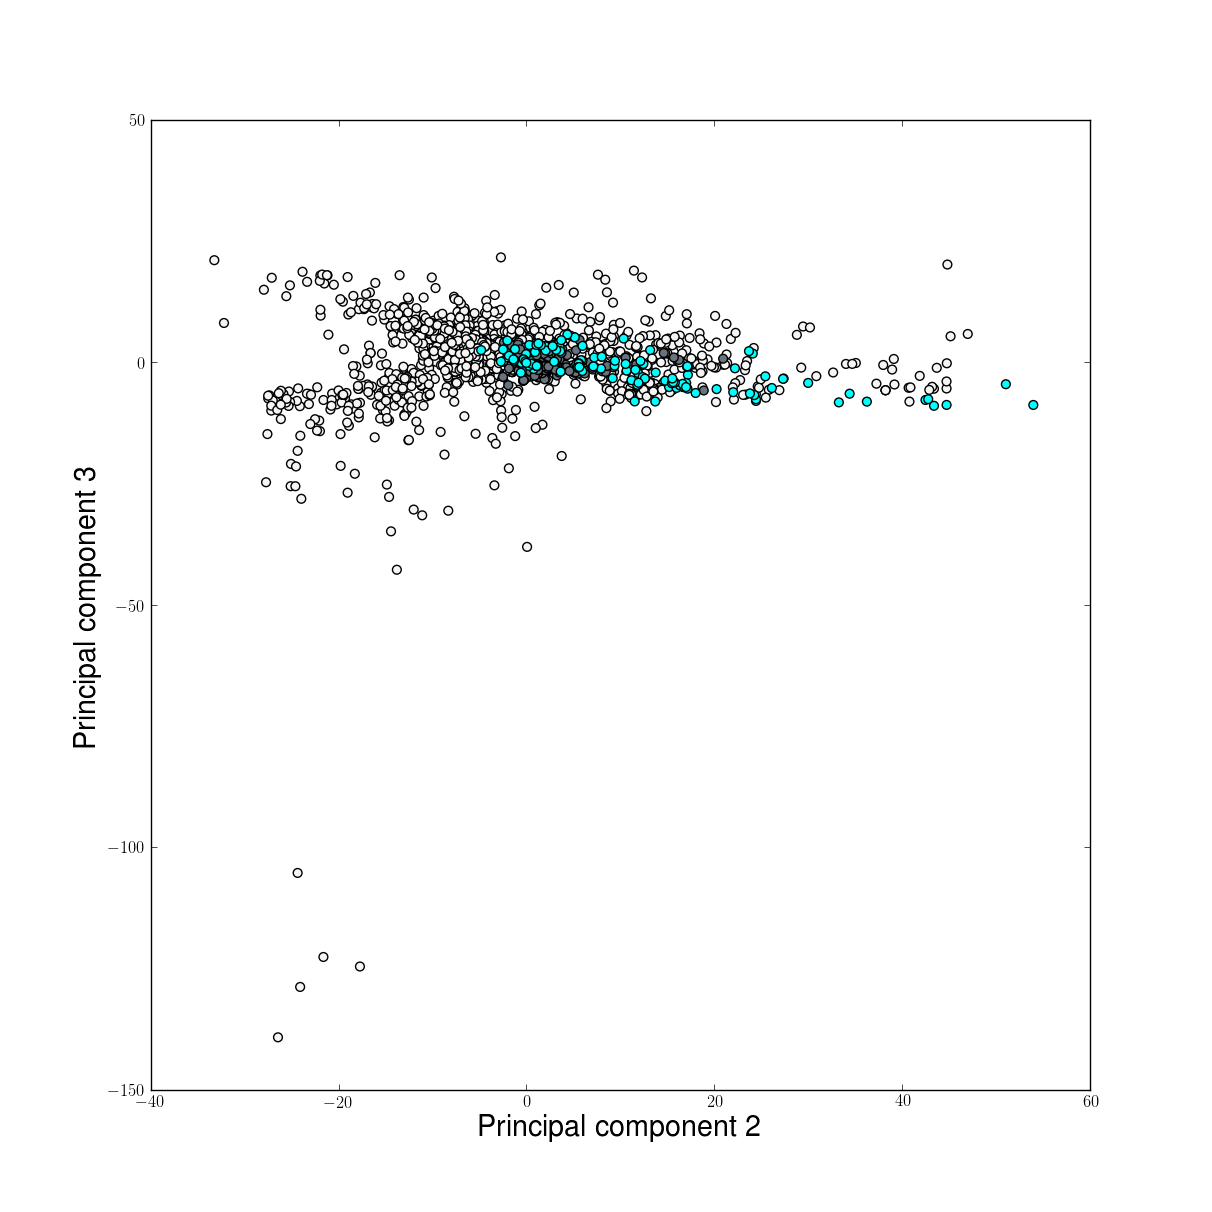
\includegraphics[width=1\textwidth]{./img/PCAcoor12.png}
	\end{subfigure}
	\begin{subfigure}[t]{0.42\textwidth}
	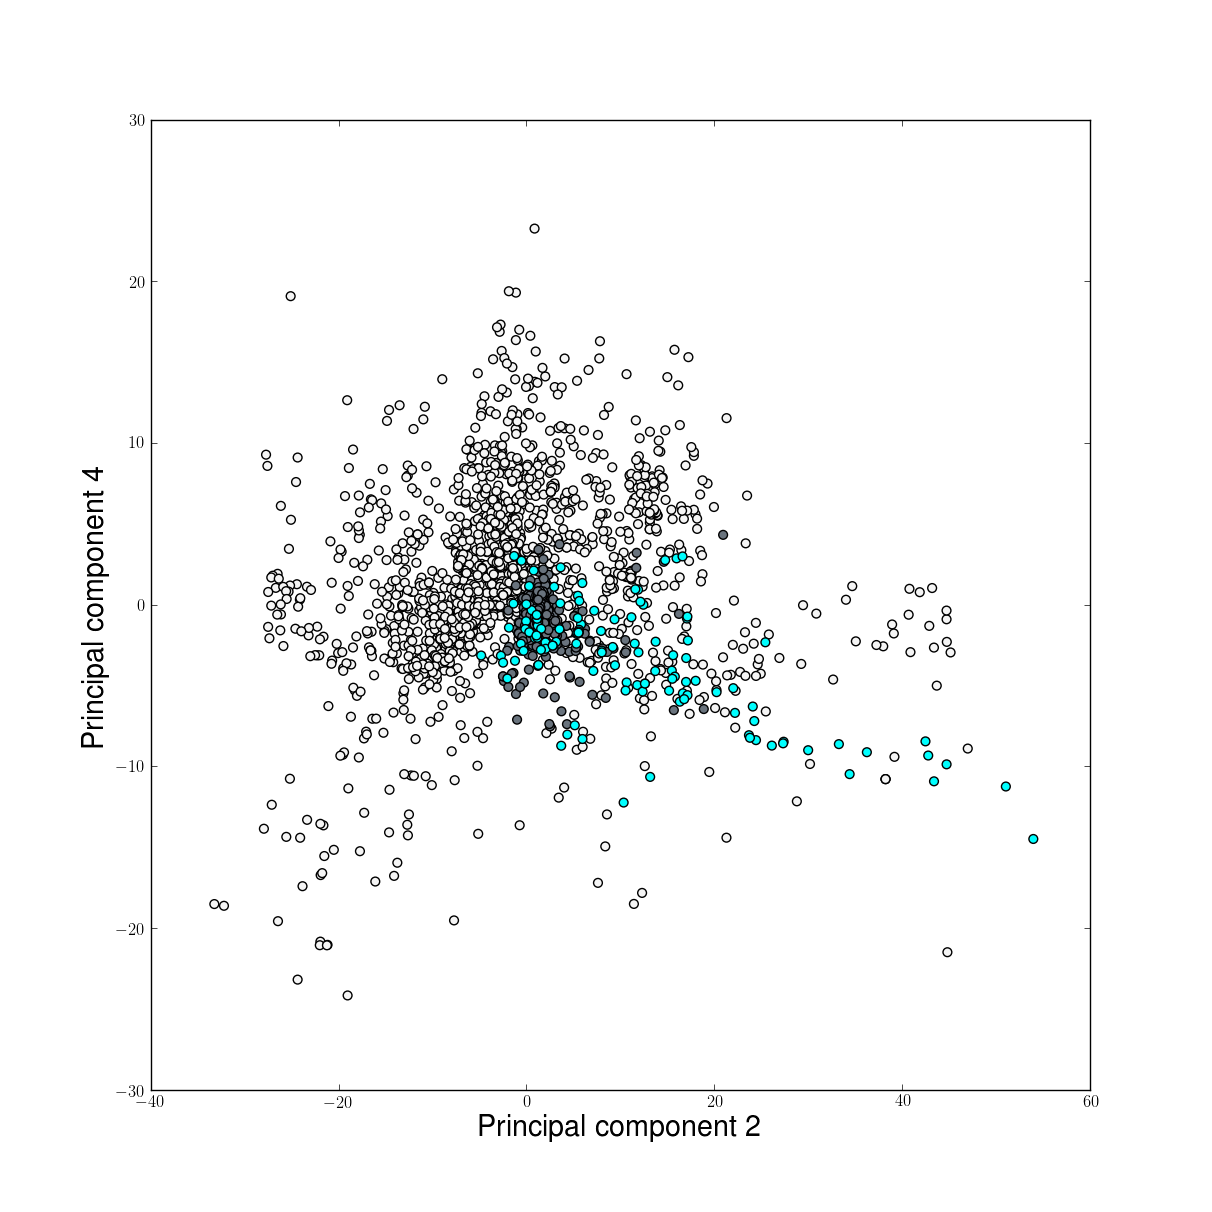
\includegraphics[width=1\textwidth]{./img/PCAcoor13.png}
	\end{subfigure}
	%\hspace{0.8cm}
	\begin{subfigure}[t]{0.42\textwidth}
	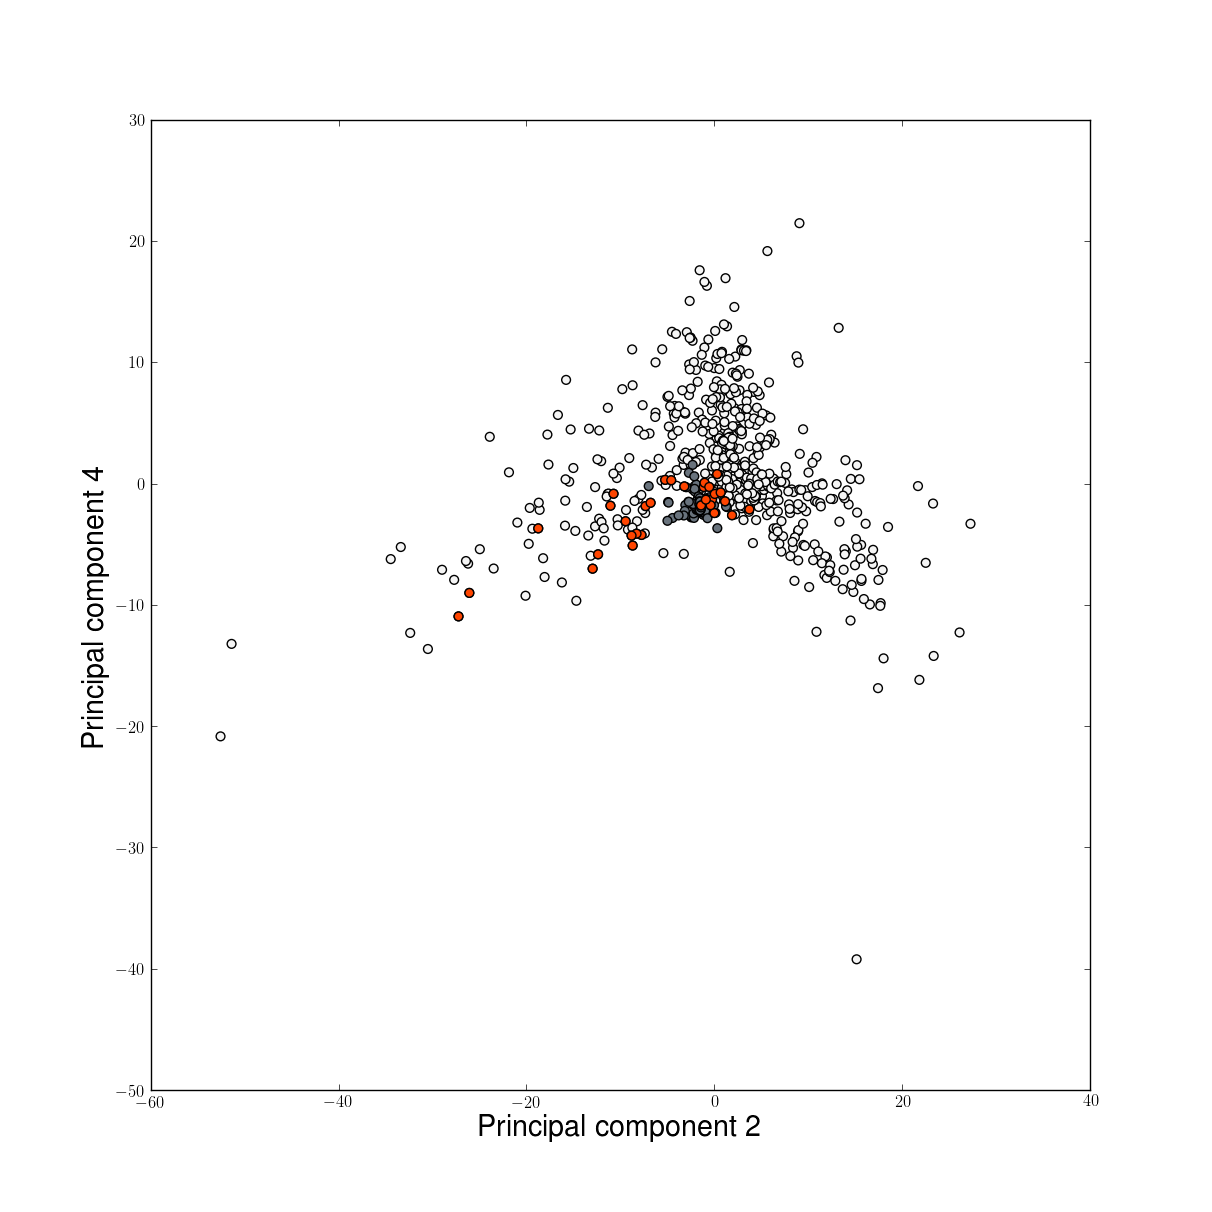
\includegraphics[width=1\textwidth]{./img/PCAncoor13.png}
	\end{subfigure}
	\begin{subfigure}[t]{0.42\textwidth}
	\includegraphics[width=1\textwidth]{./img/PCAncoor12.png}
	\end{subfigure}
	\\
	%\vspace{-0.5cm}
	\hspace{-2cm}
	\begin{subfigure}[t]{0.42\textwidth}
	\includegraphics[width=1\textwidth]{./img/PCAcoor23.png}
	\end{subfigure}
	%\hspace{0.8cm}
	\begin{subfigure}[t]{0.42\textwidth}
	\includegraphics[width=1\textwidth]{./img/PCAncoor01.png}
	\end{subfigure}
	\begin{subfigure}[t]{0.42\textwidth}
	\includegraphics[width=1\textwidth]{./img/PCAncoor02.png}
	\end{subfigure}
	\begin{subfigure}[t]{0.42\textwidth}
	\includegraphics[width=1\textwidth]{./img/PCAncoor03.png}
	\end{subfigure}
	%\vspace{-0.5cm}
	\caption[Projection fonctionnelle des réplicons selon les quatres composantes principales de l'ACP]{Projection fonctionnelle des réplicons selon les quatre premières composantes de l'ACP sur $V^{R}_{f}$ ou $V^{R}_{f}$.\\
	Chromosome : gris clair. Plasmide : gris foncé. RECE : bleu ($V^{R}_{f}$) ou rouge ($\bar{V}^{R}_{f}$).}
	\end{flushleft}
	\end{figure}
\end{landscape}
  
\fi

\newpage
\thispagestyle{empty}
\begin{figure}[H]
\vspace{-1cm}
\hspace{-2.8cm}
	\begin{minipage}{\textwidth}
	\includegraphics[trim= 0cm 2cm 0cm 0cm,clip, width=1.3\textwidth]{./img/PCA_4comp.pdf}
	\end{minipage}
\caption[Projections des réplicons selon les quatres composantes principales d'une ACP]{Projection des réplicons selon les quatre premières composantes de l'ACP sur $V^{R}_{f}$ ou $V^{R}_{f}$.\\
Chromosome : gris clair. Plasmide : gris foncé. RECE : bleu ($V^{R}_{f}$) ou rouge ($\bar{V}^{R}_{f}$).}\label{figpcascatterplot}
\end{figure}

\newpage
\begin{description}
\item[\textbullet] Les plasmides s'organisent en un groupe compact alors que différents sous-ensembles de chromosomes peuvent être identifiés (Figure \ref{figpcaproj}). Le regroupement des plasmides peut s'expliquer comme précédemment (Chapitre \ref{chap4b}), où les distances inter-plasmides sont faibles à cause du petit nombre de fonctions présentes chez eux.
\end{description}

\begin{figure}[H]
	\begin{minipage}{0.55\textwidth}
		\includegraphics[trim=2cm 7cm 2cm 6cm,clip, width=\textwidth]{./img/pca_func.png}
		\subcaption{$V^{R}_{f}$}\label{figpcavr}
	\end{minipage}
	\begin{minipage}{0.55\textwidth}
		\includegraphics[trim=2cm 7cm 2cm 6cm,clip,width=\textwidth]{./img/pca_func_ZOOM.png}
		\subcaption{ZOOM}\label{figpcavrzoom}
	\end{minipage}
	\begin{minipage}{0.55\textwidth}
		\includegraphics[trim=2cm 7cm 2cm 6cm,clip, width=\textwidth]{./img/pca_norm_func.png}
		\subcaption{$\bar{V}^{R}_{f,genre}$}\label{figpcavrnorm}
	\end{minipage}
	\begin{minipage}{0.55\textwidth}
		\includegraphics[trim=2cm 7cm 2cm 6cm,clip,width=\textwidth]{./img/pca_norm_func_ZOOM.png}
		\subcaption{ZOOM}\label{figpcavrnormzoom}
	\end{minipage}
	\begin{center}
	\caption[Visualisation des lignées bactériennes sur la projection des réplicons selon les deux composantes principales d'une ACP]{Visualisation des lignées bactériennes sur la projection des réplicons selon les deux composantes principales d'une ACP sur $V^{R}_{f}$ (\ref{figpcavr} et \ref{figpcavrzoom}) et, après normalisation taxinomique, sur $\bar{V}^{R}_{f}$ (\ref{figpcavrnorm} et \ref{figpcavrnormzoom}). \ref{figpcavrzoom} et \ref{figpcavrnormzoom}: zooms (rectangle) des figures \ref{figpcavr} et \ref{figpcavrnorm}, respectivement. Chromosome : gris clair. Plasmide : gris foncé. RECE : bleu ($V^{R}_{f}$) ou rouge ($\bar{V}^{R}_{f}$).} 
	\label{figpcaproj}
	\end{center}
\end{figure}	

\begin{description}
\item[\textbullet] Le nombre de variables positives dans un vecteur de réplicon n'est pas le seul facteur expliquant la discrimination des réplicons. En particulier, des RECE liés à peu de fonctions (tels que ceux d'\textit{Anabaena}, \textit{Butyrivibrio} ou \textit{Ilyobacter}) sont très nettement séparés des plasmides présentant un nombre de fonctions similaires (Figure \ref{figpcavrnormzoom}). Plus généralement, les RECE se différencient des plasmides et se placent de façon caractéristique par rapport aux chromosomes (Figure \ref{tabresclusterrecefunc}), à l'exception des RECE des Spirochètes (\textit{Leptospira}; Figure \ref{figpcavrnormzoom}). \textbf{\color{orange} Les RECE possèdent ainsi des spécificités fonctionnelles des STIG caractéristiques, les différenciant d'une part des chromosomes et d'autre part des plasmides}. 

\item[\textbullet]Les génomes de \textit{Prevotella} présentent un cas singulier où les chromosomes des espèces à génome multipartite \textit{(P. intermedia} et \textit{P. melaninogenica}) se distinguent de ceux des espèces à génome monopartite (\textit{P. ruminicola} et \textit{P. denticola}) en se rapprochant du groupement compact des plasmides (Figure \ref{figpcavrzoom}).

\item[\textbullet] \textbf{Sur la base de leur distribution de protéines des STIG, plusieurs types de RECE peuvent être caractérisés.} Différents niveaux de spécificité semblent exister chez les RECE, les rapprochant soit des chromosomes, soit des plasmides (Table \ref{tabresclusterrecefunc} et Figure \ref{tabrecespecificfunc}). Par exemple, les RECE des Alpha-protéobactéries semblent plus proches des chromosomes que ceux de la cyanobactérie \textit{Cyanothece} et de \textit{Candidatus} Chloroacidobacterium thermophilum (Chlorobi) qui se localisent à proximité des plasmides. Plus généralement, les résultats de ces analyses sont globalement cohérents avec les conclusions de l'étude de la totalité des réplicons (Table \ref{tabrececluster}). Les RECE ``proches" des chromosomes se retrouvent dans des clusters de chromosomes et, de même, les RECE avoisinant des plasmides (celui de \textit{Butyrivibrio} excepté) sont retrouvés dans les clusters de plasmides (Table \ref{tabrecespecificfunc}).

\item[\textbullet] \textbf{Le mode de vie des organismes bactériens influe sur les STIG de leurs réplicons génomiques.} Outre les spécificités observables de certains groupes de chromosomes de Protéobactéries, Firmicutes, Actinobactéries...(Figure \ref{figpcavr}), certains chromosomes présentent un biais de positionnement par rapport à la majorité des chromosomes et se placent à proximité des plasmides en se regroupant à leur voisinage ou avec ces derniers dans des clusters communs. Ces chromosomes appartiennent à des lignées diverses d'espèces endosymbiotiques ou de parasites/pathogènes d'eucaryotes (\textit{Rickettsia, Wolbachia, Helicobacter, Chlamydia, Mycoplasma, Borrelia, ...}). La plupart ont des tailles relativement réduites ($ \backsimeq 1 Mb$: \textit{Chlamydia}, \textit{Borrelia}...), voire très réduites ($<0.5 Mb$: \textit{Candidatus} Carsonella, \textit{Candidatus} Tremblaya...). {\bfseries \color{orange}Les génomes réduits, en adoptant une taille restreinte afin d'optimiser leur développement au sein de l'organisme hébergeant la bactérie et en relation avec la dynamique de population de la bactérie-hôte (diminution de $N_e$), développent des STIG spécifiques}. La taille n'est toutefois pas le seul facteur expliquant cette proximité. Par exemple, les génomes d'\textit{Helicobacter} (epsilon-protéobactéries) possèdent une taille relativement importante dans le contexte des génomes réduits ($\backsimeq 1.6 Mb$) mais sont fortement discriminés en comparaison à des génomes de taille similaire tels que \textit{Taylorella} (gamma-protéobactéries) ou \textit{Prochlorococcus} (Cyanobactéries).
\end{description} 

\begin{table}[H]
	\begin{center}
	\caption[Résultats de la classification non-supervisée des RECE]{Résultats de la classification non-supervisée des RECE par ACP+WARD sur $V^{R}_{f}$. Indices identiques à ceux de la Table \ref{tabrececluster}. Paramètres de l'analyse ACP+WARD décrits Table \ref{tabresclusterrecefunc}.} \label{tabrecespecificfunc} 
	\small
	\definecolor{Cchr}{RGB}{255,228,181}
	\definecolor{Cpl}{RGB}{220,220,250}
	\begin{tabular}{>{\bfseries\itshape}l|ccccccc}
		\textbf{\textnormal{Genre}} & \textbf{C} & \textbf{\footnotesize BHIw} & \textbf{\footnotesize\%chr} & \textbf{\footnotesize\%pl} & \textbf{\scriptsize\%RECE} & $E(\bigtriangleup^{r}) $ & $\bar{E}(\bigtriangleup^{C}) $ \\
		\hline
		\textit{Agrobacterium} & 3 & 0.86 & 65 & 15 & 21 & 0.95 & 0.60 \\
		\textit{Aliivibrio} & 1 & 1.00 & 0 & 30 & 70 & 0.80 & 0.70 \\
		\rowcolor{Cchr} \textit{Anabaena} & 1 & 0.21 & 77 & 19 & 4 & 0.68 & 0.64 \\
		\rowcolor{Cchr} \textit{Asticcacaulis} & 1 & 0.51 & 99 & 0 & 1 & 1.00 & 0.60 \\
		\textit{Brucella} & 1 & 0.75 & 43 & 25 & 32 & 0.98 & 0.80 \\
		\textit{Burkholderia} & 6 & 0.92 & 31 & 27 & 42 & 0.85 & 0.68 \\
		\rowcolor{Cpl} \textit{Butyrivibrio} & 1 & 0.21 & 77 & 19 & 04 & 0.68 & 0.64 \\
		\textit{Chloroacidobacterium} & 1 & 0.29 & 1 & 99 & 0 & 0.90 & 0.98 \\
		\textit{Cupriavidus} & 1 & 1.00 & 5 & 0 & 95 & 0.71 & 0.66 \\
		\rowcolor{Cpl} \textit{Cyanothece} & 1 & 0.29 & 1 & 99 & 0 & 0.90 & 0.98 \\
		\rowcolor{Cpl} \textit{Deinococcus} & 1 & 0.29 & 1 & 99 & 0 & 0.90 & 0.98 \\
		\textit{Ilyobacter} & 1 & 0.21 & 77 & 19 & 4 & 0.68 & 0.64 \\
		\rowcolor{Cpl} \textit{Leptospira} & 1 & 0.29 & 1 & 99 & 0 & 0.90 & 0.98 \\
		\textit{Nocardiopsis} & 1 & 0.21 & 77 & 19 & 4 & 0.68 & 0.64 \\
		\textit{Ochrobactrum} & 1 & 1.0 & 90 & 3 & 7 & 0.75 & 0.39 \\
		\rowcolor{Cchr} \textit{Paracoccus} & 1 & 0.89 & 92 & 3 & 5 & 0.53 & 0.32 \\
		\textit{Photobacterium} & 1 & 1.00 & 0 & 30 & 70 & 0.80 & 0.70 \\
		\rowcolor{Cchr} \textit{Prevotella} & 2 & 0.34 & 87 & 11 & 3 & 0.74 & 0.62 \\
		\textit{Pseudoalteromonas} & 1 & 0.21 & 77 & 19 & 4 & 0.68 & 0.64 \\
		\textit{Ralstonia} & 2 & 1.00 & 11 & 22 & 77 & 0.77 & 0.69 \\
		\rowcolor{Cpl} \textit{Rhodobacter} & 2 & 0.84 & 27 & 41 & 32 & 0.97 & 0.73 \\
		\rowcolor{Cpl} \textit{Sinorhizobium} & 2 & 0.86 & 25 & 27 & 48 & 0.87 & 0.76 \\
		\textit{Sphaerobacter} & 1 & 0.35 & 100 & 0 & 0 & 1.00 & 0.60 \\
		\rowcolor{Cpl} \textit{Sphingobium} & 2 & 34 & 64 & 27 & 9 & 0.84 & 0.64 \\
		\textit{Thermobaculum} & 1 & 0.21 & 77 & 19 & 4 & 0.68 & 0.64 \\
		\textit{Variovorax} & 1 & 1.00 & 0 & 30 & 70 & 0.80 & 0.70 \\
		\textit{Vibrio} & 4 & 0.97 & 31 & 32 & 37 & 0.83 & 0.57 \\
	\end{tabular}
	\end{center}
\end{table}	

\section{Discrimination fonctionnelle des génomes} 

	La même analyse a été appliquée aux génomes ($V_{f}^{G}$ et $\bar{V}_{f,genre}^{G}$). L'ACP a été utilisée pour projeter les données dans un espace de dimension réduite afin de les visualiser et les clusteriser. Les quatre principales composantes ont de plus été utilisées pour la classification par WARD. Le choix de $k$ pour l'analyse de clustering est fondé sur le critère de stabilité $\bigtriangleup^{Kl}$ (éq. \ref{eqestimstaball}) pour $k \in \{3,10,20,50,70,100,150\}$. 
	 
\begin{table}[H]
	\begin{center}
	\caption[Évaluation du clustering fonctionnel des génomes.]{Évaluation du clustering fonctionnel des génomes.} 	\label{tabresclustergenomefunc}
	\begin{tabular}{l|l|cccc}
		& \textbf{Indices$^{a}$}  & \multicolumn{2}{c}{\textbf{ACP+WARD}}   \\
		\hline
		& & & &  \\[-0.2cm]
		Données &  & $V_{f}^{G}$ & $\bar{V}_{f,genre}^{G}$  \\
		\multirow{2}{*}{Paramètres de WARD $^{b}$} &  & \textit{k}: 150  & \textit{k}: 70  \\
		&  & \textit{cp}: 4 & \textit{cp}: 4 \\
		Nombre de clusters ACP &  & 142 & 60 \\
		Variance expliquée ACP & & 82\% & 81\% \\
		\hline
		 & & & &  \\[-0.2cm]
		\textbf{Critère de stabilité$^{c}$} $\bigtriangleup^{Kl}$ &  & 0.68 & 0.58  \\
		\hline
		\multirow{3}{*}{\textbf{Type de génome}} & \textit{homogeneity} & 0.60 & 0.39  \\
		& \textit{completeness} & 0.03 & 0.02 \\
		& \textit{V-measure} & 0.05 & 0.04 \\
		\hline
		\multirow{3}{*}{\textbf{Phylum des génomes}} & \textit{homogeneity} & 0.51 & 0.55 \\
		& \textit{completeness} & 0.22 & 0.29 \\
		& \textit{V-measure} & 0.31 & 0.38 \\
		\hline
		\multirow{3}{*}{\textbf{Classe des génomes}} & \textit{homogeneity} & 0.51 & 0.51 \\
		& \textit{completeness} & 0.32 & 0.39 \\
		& \textit{V-measure} & 0.39 & 0.44 \\
	\end{tabular}
	\medskip
	\captionsetup{justification=justified}
	\caption*{\footnotesize {$^{a}$ \textit{V-measure} calculée selon l'éq. \ref{eqvm}. \\ $^{b}$ $k$, nombre de clusters en \textit{input} et $cp$, nombre de composantes principales retenues pour la classification par WARD. \\ $^{c}$ Critère de stabilité $\bigtriangleup^{Kl}$ calculé par l'éq. \ref{eqestimstaball}}}.
	\captionsetup{}
	\end{center}
 \end{table}

	 Les clusters de génomes obtenus par ACP+WARD sont plus instables que ceux obtenus pour les réplicons (Table \ref{tabresclustergenomefunc}) et sont donc difficilement interprétables et potentiellement fortement bruités. Les critères d'\textit{homogeneity} indiquent de plus qu'il n'y a \textit{a priori} pas de séparation nette détectable entre génomes mono- et multipartites. Cependant, les projections des données selon les quatre composantes principales de l'ACP sont pertinentes compte-tenu de la variabilité expliquée ($>80\%$, Table \ref{tabresclustergenomefunc}). De plus, les projections de $\bar{V}_{f,genre}^{G}$ montrent des tendances similaires à celles de $V_{f}^{G}$ (Figure \ref{figpcagenome}). \\
 		

\begin{figure}
	\begin{minipage}{0.55\textwidth}
		\includegraphics[trim=2cm 7cm 2cm 6cm,clip, width=\textwidth]{./img/pca_genome.png}
		\subcaption{$V^{G}_{f}$}\label{figpcavg}
	\end{minipage}
	\begin{minipage}{0.55\textwidth}
		\includegraphics[trim=2cm 7cm 2cm 6cm,clip,width=\textwidth]{./img/pca_genome_II.png}
		\subcaption{$V^{G}_{f}$}\label{figpcavg2}
	\end{minipage}
	\begin{center}
	\begin{minipage}{0.55\textwidth}
		\includegraphics[trim=2cm 7cm 2cm 6cm,clip,width=\textwidth]{./img/pca_genome_norm.png}
		\subcaption{$\bar{V}^{G}_{f,genre}$}\label{figpcavg3}
	\end{minipage}
	\caption[Projection fonctionnelle des génomes selon les deux composantes principales d'une ACP ]{Projection fonctionnelle des génomes selon les deux composantes principales d'une ACP sur $V^{G}_{f}$ (A,B) ou  $\bar{V}^{G}_{f,genre}$ (C). \\ Génomes monopartites : gris foncé; génomes multipartites: magenta. Bêtaprotéobactéries: kaki, Alphaprotéobactéries: vert.\\
A: Visualisation de la tendance de répartition des Bêta-protéobactéries (rose) et de groupes majoritairement formés de génomes monopartites (jaune). B: Visualisation des localisations des génomes monopartites des Bêtaprotéobactéries et des Alphaprotéobactéries (Rhizobiales indiquées par des marqueurs carré). Rectangle rouge à droite de la figure: génomes uniquement composés de plasmides. C: Visualisation des génomes multipartites les plus différenciés parmi les Bêtaprotéobactéries (kaki) et les Alphaprotéobactéries (vert) selon une projection de $\bar{V}^{G}_{f,genre}$ sur les deux composantes principales.} \label{figpcagenome}
	\end{center}
\end{figure}
	  	

\begin{description}
	\item[\textbullet] \textbf{Aucune tendance générale ne caractérise les génomes multipartites dans leur globalité}. Les variables utilisées ne permettent pas de mettre en avant une discrimination significative des génomes multipartites par rapport aux génomes monopartites (Table \ref{tabresclustergenomefunc}). D'éventuelles spécificités des génomes qui, à l'échelle des réplicons étaient clairement visibles, sont peut-être “noyées” dans la masse des données génomiques. Alternativement, il est possible que l'on ne dispose de pas suffisamment de variables pour qu’émerge une tendance caractéristique des génomes multipartites.
	
	\item[\textbullet] \textbf{Certains génomes, dont une part importante de génomes multipartites, sont cependant clairement discriminés.} Les projections indiquent que certains génomes s'écartent de l'ensemble des génomes (Figure \ref{figpcagenome}). Ils englobent les génomes multipartites des Bêtaprotéobactéries ainsi qu'une part importante des génomes des Rhizobiales (Alphaprotéobactéries). Ces génomes appartiennent majoritairement à des espèces associées à des plantes, parmi lesquelles des pathogènes mais surtout des mutualistes qui sont connus pour échanger des gènes impliqués dans le développement de l'association symbiotique aux plantes. Au-delà des gènes impliqués dans la symbiose avec un hôte eucaryote, \textbf{\color{orange} l'écologie particulière de ces organismes (symbiotes des plantes) est corrélée à une adaptation spécifique des STIG de ces génomes}. Cette corrélation n'étant pas détectable sur les analyses des réplicons (Figure \ref{figpcaproj}), on peut proposer l'hypothèse corollaire que \textbf{\color{orange} cette adaptation des STIG passe par l'adaptation des réplicons extra-chromosomiques}. Ces hypothèses sont toutefois à considérer avec prudence, compte tenu de l'instabilité des données, et seront à confirmer ou infirmer par des analyses complémentaires.
\end{description}
	 
	
\section{Analyses par régression et test d'hypothèses}
 	L'identification des différents biais fonctionnels des groupements de réplicons ou de génomes conduit naturellement à tenter d'identifier les fonctions impliquées dans la discrimination de ces groupes. Pour comparer les groupes d'éléments génomiques, nous avons réalisé une régression logistique sur les distributions des 117 fonctions de notre analyse. Deux critères sont considérés: la \textbf{\textit{$P_{value}$}} mesurant la capacité d'une fonction à être spécifique d'une classe donnée et l'\textbf{\textit{Odd-Ratio}} évaluant, pour une observation donnée, l'influence de la présence d'une fonction sur l'appartenance de cette observation à une classe donnée.

\subsection{Régression logistique: principe}\label{parregresslog}
	Pour un ensemble $E$ d'observations expliquées par $n$ attributs, organisé en deux sous-ensembles tels que $E=E_{True}\cup E_{False}$, $E_{training}=\{E_{True},E_{False}\}$ représente une procédure de régression logistique simple, assimilable à une procédure de classification supervisée binaire $f_{reg}^{E_{training}}$ où:

	\begin{equation}\label{eqlogreg}
		f_{reg}^{E_{training}}(o)=\frac{e^{\beta_{0}+\sum_{1\leq i \leq |v_{o}|}\beta_{i} v_{o}[i]}}{1+e^{\beta_{0}+\sum_{1\leq i \leq |v_{o}|}\beta_{i} v_{o}[i]}}, \: o \in E
	\end{equation}

avec $v_{o}$, le vecteur associé à l'observation $o$ et $\beta_{i}$, les coefficients de la fonction \textit{logit} définie par:

	\begin{equation}
		g(o)=ln\left(\frac{f_{reg}^{E_{training}}(o)}{1-f_{reg}^{E_{training}}(o)}\right)=\beta_{0}+\sum_{1\leq i \leq |v_{o}|}\beta_{i}.v_{o}[i] 
	\end{equation}

Les $\beta_{i}$ sont alors estimés afin de proposer le modèle expliquant au mieux les observations de $E_{training}$, de telle sorte que $f_{reg}^{E_{training}}(o)\approx 1$ pour $o \in E_{True}$ et $f_{reg}^{E_{training}}(o)\approx 0$ pour $o \in E_{False}$ \citep{hosmer2013applied}. $f_{reg}^{E_{training}}(o)$ étant inclus dans l'intervalle $]0,1[$, cette valeur peut être considérée comme la probabilité qu'$o$ appartiennent à $E_{True}$ \citep{Larose2006}. La signifiance du modèle, ou des coefficients $\beta_{i}$, peut alors être estimée \textit{via} des tests statistiques sur la \textit{deviance} du modèle ou en applicant le test de Wald individuellement sur chaque coefficient \citep{Larose2006}. Le test de Wald, en particulier, évalue si un coefficient $\beta_{i}$ est significativement différent de $0$. Dans de cas d'observations ayant un unique attribut dichotomique (deux valeurs possibles), le rapport de chance (ou \textit{\textbf{O}dd \textbf{R}atio} ($OR$)) \citep{Larose2006} est défini par:

	\begin{equation}
		\begin{split}
		OR & =\frac{\frac{f_{reg}^{E_{training}}(1)}{1-f_{reg}^{E_{training}}(1)}}{\frac{f_{reg}^{E_{training}}(0)}{1-f_{reg}^{E_{training}}(0)}}=e^{\beta_{1}} \\
		% & =e^{\beta_{1}}
		\end{split}
	\end{equation}

Un OR de 5,0 pour un modèle de \textit{logit} défini sur un ensemble d'observations univariées prenant leur valeur dans $\{0,1\}$ indiquera que, selon le modèle de régression, les observations prenant la valeur 1 auront 5 fois plus de chances d'être dans la catégorie $E_{True}$ que les observations ayant comme valeur $0$. Pour des observations univariées continues suivant l'hypothèse que $\beta_{1}$ est constant, le rapport de chance $e^{\beta_{1}}$ est alors l'augmentation de chance d'appartenir à $E_{True}$ suivant l'augmentation des valeurs des observations d'une unité \citep{hosmer2013applied}. \\


\subsection{Jeux de données}\label{parregjeuxdedonnee}
Différentes classes de référence $K_{i}$ d'ensembles de réplicons ont été formées (Table \ref{tabclassecaracter}).  Les génomes incomplets, ne contenant pas de chromosomes, ne sont pas pris en considération. D'une manière générale, les données sont systématiquement normées par genre taxonomique afin d'éviter les corrélations dues à la sur-représentation de certains genres bactériens. Bien qu'il semble exister plusieurs types différenciés, les RECE ont été rassemblés dans une unique classe de référence $K_{RECE}$, le nombre d'observations n'étant pas suffisant pour permettre la création de plusieurs classes. La classe de référence $K_{plasmide}$ rassemble l'ensemble des plasmides et la classe $K_{chr}$ regroupe l'ensemble des chromosomes. Les classes $K_{monopartite}$ et $K_{multipartite}$ regroupent, respectivement, l'ensemble des génomes monopartites et celui des génomes multipartites. Soit $G_{alphaproteo}$ et $G_{betaproteo}$ les ensembles des génomes des classes Alphaprotéobactéries et Bêtaprotéobactéries, respectivement. Les classes $K_{alphamono}$, $K_{alphamulti}$, $K_{betamono}$, $K_{betamulti}$ sont alors formées \underline{sans} normer les observations par genre taxonomique, les espèces étant alors l'objet de la comparaison. 

\begin{table}

	\begin{center}
	\caption[Propriétés des classes utilisées pour l'analyse de régression logistique]{Propriétés des classes utilisées pour l'analyse par régression logistique.}\label{tabclassecaracter}
 	\begin{tabular}{ccc}
	\textbf{Classe} & \textbf{Données$^{a}$} & \textbf{Taille$^{b}$} \\
	\hline
	 & &  \\[-0.2cm]
	$K_{RECE}$ & $\bar{V}^{R^{\{RECE\}}}_{f,genre}$ & (31,117) \\
	 & &  \\[-0.2cm]
	$K_{plasmide}$ & $ \bar{V}^{R^{\{plasmide\}}}_{f,genre}$ & (273,117) \\
	 & &  \\[-0.2cm]
	$K_{chr}$ & $\bar{V}^{R^{\{chr\}}}_{f,genre}$ & (546,117) \\
	 & &  \\[-0.2cm]
	$K_{monopartite}$ & $\bar{V}^{G^{\{monopartite\}}}_{f,genre}$ & (530,117) \\
	 & &  \\[-0.2cm]
	$K_{multipartite}$ & $\bar{V}^{G^{\{monopartite\}}}_{f,genre}$ & (29,117) \\
	 & &  \\[-0.2cm]
	$K_{alphamono}$ & $V^{G_{alphaproteo}^{\{monopartite\}}}_{f}$ & (186,117) \\
	 & &  \\[-0.2cm]
	$K_{alphamulti}$ & $V^{G_{alphaproteo}^{\{multipartite\}}}_{f}$ & (32,117) \\
	 & &  \\[-0.2cm]
	$K_{betamono}$ & $V^{G_{betaproteo}^{\{monopartite\}}}_{f}$ & (93,117) \\
	 & &  \\[-0.2cm]
	$K_{betamulti}$ & $V^{G_{betaproteo}^{\{multipartite\}}}_{f}$ & (40,117) \\
	\end{tabular}
	\medskip
	\captionsetup{justification = justified}	
	\caption*{$^{a}$: Les notations utilisées sont celles introduites précédemment (\S \ref{pardonnee2} et \ref{parregjeuxdedonnee}), $R$ représentant l'ensemble des réplicons. \\ $^{b}$: dimensions de la matrice associée aux données.}
	\captionsetup{}
	\end{center}
\end{table}

	Nous avons donc étudié par régression logistique la pertinence des fonctions des STIG pour représenter ces différentes classes de réplicons. Les chromosomes sont comparés aux plasmides puis aux RECE. Les RECE sont ensuite comparés aux plasmides. Enfin, pour approfondir les résultats de discrimination fonctionnelle des réplicons par ACP+WARD (\S \ref{pardiscriminfuncrepl}), les génomes monopartites et multipartites sont comparés à l'intérieur des Bêtaprotéobactéries et des Alphaprotéobactéries, respectivement.
		
\subsection{Résultats et discussion}\label{reglogresult}
Les régressions logistiques ont été réalisées pour des couples d'ensembles d'observations univariées et continues. Les $OR$ sont tous calculés pour des observations ayant des attributs continus et indiquent l'augmentation de probabilité, selon le modèle estimé, qu'une observation appartienne à une classe donnée pour l'augmentation d'une unité de la valeur de l'attribut considéré. Par exemple, pour l'étude de la fonction \textit{ACLAME RepA E B} entre les classes $K_{betamono}$ et $K_{betamulti}$, un $OR$ de 7,7 est estimé avec une $P_{value}$ de $4,1 * 10^{-9}$ (Table \ref{tabreglogis}), ce qui signifie qu'un génome ayant 2 gènes codant pour des protéines annotées \textit{RepA, RepE, RepB} dans ACLAME aura $7,7 * 2=15,4$ fois plus de chances d'être un génome multipartite qu'un génome ne possédant aucun gène codant des protéines \textit{RepAEB}. Pour l'étude entre $K_{chr}$ et $K_{plasmide}$, un ensemble de réplicons normés par genre taxonomique où la moitié des réplicons possèdent des gènes codant des protéines annotées \textit{ParA, ParM} dans ACLAME aura $0,5 * 0,4 = 0,2$ fois plus de chance d'être un ensemble de chromosomes qu'un ensemble où aucun des réplicons ne possède de tels gènes. Ces modèles de régression reposent cependant sur l'hypothèse que les coefficients $\beta_{1}$ sont constants, ce qui peut s'avérer faux dans certains cas. Par exemple, la probabilité pour un réplicon d’acquérir un gène d'une source externe est vraisemblablement différente de celle qu'un gène existant se duplique.

\begin{landscape}
\thispagestyle{empty}
\definecolor{posit}{RGB}{163,239,176}
\definecolor{posit2}{RGB}{225,250,229}
\definecolor{colorpower}{RGB}{255,255,224}
\definecolor{colorpowerx}{RGB}{245,222,179}
\definecolor{colorpowerxx}{RGB}{222,184,135}
\definecolor{colorpowerxxx}{RGB}{244,164,96}
\definecolor{colorpowerxxxx}{RGB}{210,105,30}

\definecolor{colorpowerneg}{RGB}{208,243,246}
\definecolor{colorpowernegx}{RGB}{157,232,238}
\definecolor{colorpowernegxx}{RGB}{97,218,226}
\definecolor{colorpowernegxxx}{RGB}{9,218,223}
\definecolor{colorpowernegxxxx}{RGB}{7,146,252}


\begin{table}
\vspace{-3.5cm}
\hspace{-2cm}
\scalebox{0.45}{\begin{minipage}[t]{0.3\textwidth}
	\vspace{0cm}
	\subcaption*{\huge\hspace{1.5cm} $\:\:K_{chr}$/$K_{plasmide}$}
		\vspace{0.5cm}
	\begin{tabular}{>{\bfseries}p{\textwidth}cc}
\textbf{Fonction}& \textbf{$P_{value}^{a}$} & \textbf{OR}$^{b}$\\
\hline
\\[-0.1cm]
\rowcolor{posit}kegg hupB&1.2e-53&\textbf{\colorbox{colorpowerxxxx}{97.6}}\\
\rowcolor{posit}kegg dnaG&2.1e-50&\textbf{\colorbox{colorpowerxxxx}{1861.5}}\\
\rowcolor{posit}kegg parB spo0J&2.5e-44&\textbf{\colorbox{colorpowerxx}{13.7}}\\
\rowcolor{posit}kegg dnaA&3.0e-44&\textbf{\colorbox{colorpowerxxxx}{2118.9}}\\
\rowcolor{posit}kegg dnaB&1.1e-43&\textbf{\colorbox{colorpowerxxxx}{1992.9}}\\
\rowcolor{posit}kegg xerC&1.7e-43&\textbf{\colorbox{colorpowerxxxx}{55.0}}\\
\rowcolor{posit}kegg ssb&5.9e-41&\textbf{\colorbox{colorpowerxxxx}{298.3}}\\
\rowcolor{posit}kegg xerD&1.3e-38&\textbf{\colorbox{colorpowerxxx}{26.6}}\\
\rowcolor{posit}kegg parA soj&2.7e-38&\textbf{\colorbox{colorpowerxx}{9.9}}\\
\rowcolor{posit}kegg ftsK spoIIIE&2.8e-37&\textbf{\colorbox{colorpowerxxxx}{76.9}}\\
\rowcolor{posit}kegg E3.5.1.28B amiA amiB amiC&6.4e-36&\textbf{\colorbox{colorpowerxxx}{46.4}}\\
\rowcolor{posit}kegg scpB&7.5e-32&\textbf{\colorbox{colorpowerxxxx}{102.5}}\\
\rowcolor{posit}kegg ftsZ&3.1e-31&\textbf{\colorbox{colorpowerxxxx}{2747.0}}\\
\rowcolor{posit}aclame Helicase&1.6e-27&\textbf{\colorbox{colorpowerxxxx}{71.1}}\\
\rowcolor{posit}kegg parC&3.0e-27&\textbf{\colorbox{colorpowerxxxx}{4149.3}}\\
\rowcolor{posit}kegg cbpA&8.2e-27&\textbf{\colorbox{colorpowerxxxx}{2608.4}}\\
\rowcolor{posit}kegg parE&7.3e-26&\textbf{\colorbox{colorpowerxxxx}{5842.4}}\\
\rowcolor{posit}kegg ftsE&4.2e-24&\textbf{\colorbox{colorpower}{2.3}}\\
\rowcolor{posit}kegg mreB&1.3e-21&\textbf{\colorbox{colorpowerxxxx}{1598.2}}\\
\rowcolor{posit}aclame DNAhelicase&5.8e-21&\textbf{\colorbox{colorpowerxxx}{33.6}}\\
\rowcolor{posit}kegg dps&9.1e-21&\textbf{\colorbox{colorpowerxxxx}{65.3}}\\
\rowcolor{posit}aclame ATPase.tyrK.exoP&2.2e-20&\textbf{\colorbox{colorpowerxx}{19.4}}\\
\rowcolor{posit}kegg iciA&7.1e-20&\textbf{\colorbox{colorpowerx}{3.2}}\\
\rowcolor{posit}kegg lrp&1.6e-19&\textbf{\colorbox{colorpowerxx}{8.4}}\\
\rowcolor{posit}kegg minD&3.1e-19&\textbf{\colorbox{colorpowerxxx}{42.8}}\\
\rowcolor{posit}kegg rob&6.3e-19&\textbf{\colorbox{colorpowerx}{5.3}}\\
\rowcolor{posit}kegg acrA&6.6e-19&\textbf{\colorbox{colorpowerx}{2.8}}\\
\rowcolor{posit}kegg mrp&6.6e-17&\textbf{\colorbox{colorpowerxxxx}{2599.3}}\\
\rowcolor{posit}kegg gidB rsmG&6.7e-17&\textbf{\colorbox{colorpowerxxxx}{6059.9}}\\
\rowcolor{posit}aclame RepA E B&1.7e-16&\textbf{\colorbox{colorpowernegxxx}{0.0}}\\
\rowcolor{posit}kegg ftsW spoVE&5.7e-16&\textbf{\colorbox{colorpowerxxxx}{4266.4}}\\
\rowcolor{posit}kegg dam&6.9e-16&\textbf{\colorbox{colorpowerxx}{16.7}}\\
\rowcolor{posit}kegg diaA&1.5e-15&\textbf{\colorbox{colorpowerxxxx}{81.9}}\\
\rowcolor{posit}kegg ftsQ&1.7e-15&\textbf{\colorbox{colorpowerxxxx}{2135.0}}\\
\rowcolor{posit}aclame PSK higBA&3.3e-15&\textbf{\colorbox{colorpowerx}{3.4}}\\
\rowcolor{posit}kegg ihfB himD&1.2e-14&\textbf{\colorbox{colorpowerxxxx}{68.4}}\\
\rowcolor{posit}kegg gidA mnmG MTO1&5.2e-13&\textbf{\colorbox{colorpowerxxxx}{1477.2}}\\
\rowcolor{posit}kegg hfq&1.4e-12&\textbf{\colorbox{colorpowerxxxx}{121.7}}\\
\rowcolor{posit}kegg ihfA himA&1.7e-12&\textbf{\colorbox{colorpowerxxxx}{63.8}}\\
\rowcolor{posit}kegg rodA mrdB&2.8e-12&\textbf{\colorbox{colorpowerxxxx}{1233.1}}\\
\rowcolor{posit}aclame ParB&5.7e-12&\textbf{\colorbox{colorpowernegxx}{0.1}}\\
\rowcolor{posit}kegg dnaC&6.0e-12&\textbf{\colorbox{colorpower}{2.6}}\\
\rowcolor{posit}kegg ftsX&9.3e-12&\textbf{\colorbox{colorpowerxxxx}{972.9}}\\
\rowcolor{posit}kegg ftsA&9.5e-12&\textbf{\colorbox{colorpowerxxxx}{742.7}}\\
\rowcolor{posit}aclame PSK mazEF&1.2e-11&\textbf{\colorbox{colorpowerx}{5.2}}\\
\rowcolor{posit}kegg scpA&1.4e-11&\textbf{\colorbox{colorpowerxxxx}{789.4}}\\
\rowcolor{posit}kegg mreC&2.9e-11&\textbf{\colorbox{colorpowerxxxx}{1311.2}}\\
\rowcolor{posit}aclame XerTyrosine&7.6e-11&\textbf{\colorbox{colorpower}{2.0}}\\
\rowcolor{posit}aclame ParA.ParM&1.5e-10&\textbf{\colorbox{colorpowernegx}{0.4}}\\
\rowcolor{posit}aclame PSK vapBC.vag&1.2e-09&\textbf{\colorbox{colorpowerx}{3.9}}\\
\rowcolor{posit}kegg fic&3.1e-09&\textbf{\colorbox{colorpowerxx}{10.3}}\\
\rowcolor{posit}kegg slmA ttk&3.8e-09&\textbf{\colorbox{colorpowerxxx}{52.3}}\\
\rowcolor{posit}kegg minC&4.4e-09&\textbf{\colorbox{colorpowerxxxx}{172.3}}\\
\rowcolor{posit}kegg zapA&8.2e-09&\textbf{\colorbox{colorpowerxxxx}{602.8}}\\
\rowcolor{posit}kegg minE&9.0e-09&\textbf{\colorbox{colorpowerxxxx}{152.9}}\\
\rowcolor{posit}kegg ftsI&9.8e-09&\textbf{\colorbox{colorpowerxxx}{47.0}}\\
\rowcolor{posit}aclame RuvB&1.2e-08&\textbf{\colorbox{colorpowerxxxx}{433.0}}\\
\rowcolor{posit}kegg smc&1.6e-08&\textbf{\colorbox{colorpowerxxxx}{3090.5}}\\
\rowcolor{posit}kegg mreD&1.8e-08&\textbf{\colorbox{colorpowerxxxx}{459.2}}\\
\rowcolor{posit}aclame PSK relBE&2.7e-08&\textbf{\colorbox{colorpowerx}{3.5}}\\
\rowcolor{posit}aclame PSK parDE&5.5e-08&\textbf{\colorbox{colorpower}{2.3}}\\
\rowcolor{posit}kegg sepF&1.8e-07&\textbf{\colorbox{colorpowerxxxx}{68.8}}\\
\rowcolor{posit}aclame FtsK.SpoIIIE&1.9e-07&\textbf{\colorbox{colorpowerx}{6.0}}\\
\rowcolor{posit}aclame PSK phD.doc&3.2e-07&\textbf{\colorbox{colorpowerxx}{11.9}}\\
\rowcolor{posit}kegg fis&5.8e-07&\textbf{\colorbox{colorpowerxxxx}{180.9}}\\
\rowcolor{posit}kegg hda&7.3e-07&\textbf{\colorbox{colorpowerxxxx}{149.1}}\\
\rowcolor{posit}kegg ftsB&1.1e-06&\textbf{\colorbox{colorpowerxxxx}{167.2}}\\
\rowcolor{posit}kegg trmFO gid&1.5e-06&\textbf{\colorbox{colorpowerxxxx}{182.5}}\\
\rowcolor{posit}aclame serinerecombinase&2.5e-06&\textbf{\colorbox{colorpower}{1.4}}\\
\end{tabular}
	\end{minipage}}
	\hspace{1.7cm}
\scalebox{0.45}{\begin{minipage}[t]{0.3\textwidth}
	\vspace{0cm}
	\subcaption*{\huge\hspace{1cm} (suite) }
		\vspace{0.5cm}
	\begin{tabular}{>{\bfseries}p{\textwidth}cc}
	\textbf{Fonction}& \textbf{$P_{value}$} & \textbf{OR}\\
\hline
\\[-0.1cm]
	\rowcolor{posit}kegg sulA&3.3e-06&\textbf{\colorbox{colorpowerxx}{17.5}}\\
\rowcolor{posit}kegg divIVA&4.1e-06&\textbf{\colorbox{colorpowerxxxx}{128.0}}\\
\rowcolor{posit}kegg hns&1.1e-05&\textbf{\colorbox{colorpowerx}{2.8}}\\
\rowcolor{posit}kegg ftsL&1.2e-05&\textbf{\colorbox{colorpowerxxxx}{91.5}}\\
\rowcolor{posit}aclame PSK HicAB&4.3e-05&\textbf{\colorbox{colorpowerxxx}{25.2}}\\
\rowcolor{posit}kegg divIC divA&4.9e-05&\textbf{\colorbox{colorpowerxxxx}{90.5}}\\
\rowcolor{posit}kegg zipA&7.9e-05&\textbf{\colorbox{colorpowerxxxx}{66.0}}\\
\rowcolor{posit}kegg ftsN&1.6e-04&\textbf{\colorbox{colorpowerxxx}{53.0}}\\
\rowcolor{posit}aclame DNArepair&2.2e-04&\textbf{\colorbox{colorpowerxxx}{34.0}}\\
\rowcolor{posit}kegg hupA&2.7e-04&\textbf{\colorbox{colorpowerxx}{15.1}}\\
\rowcolor{posit}aclame TyrosinerecOrfA&3.4e-04&\textbf{\colorbox{colorpowerx}{3.3}}\\
\rowcolor{posit}kegg seqA&1.6e-03&\textbf{\colorbox{colorpowerxxx}{25.9}}\\
\rowcolor{posit}kegg mukB&2.3e-03&\textbf{\colorbox{colorpowerxxx}{27.4}}\\
\rowcolor{posit}kegg mukE&3.1e-03&\textbf{\colorbox{colorpowerxxx}{21.0}}\\
\rowcolor{posit}kegg mukF&3.7e-03&\textbf{\colorbox{colorpowerxx}{19.6}}\\
\rowcolor{posit}kegg dnaI&5.2e-03&\textbf{\colorbox{colorpowerxx}{18.0}}\\
\rowcolor{posit}aclame RepA&5.9e-03&\textbf{\colorbox{colorpowerneg}{0.7}}\\
\rowcolor{posit}kegg dnaB2 dnaB&6.7e-03&\textbf{\colorbox{colorpowerxx}{12.6}}\\
\\
\rowcolor{posit2}kegg ezrA&1.0e-02&\textbf{\colorbox{colorpowerxx}{13.7}}\\
\rowcolor{posit2}aclame RepR S E&1.3e-02&\textbf{\colorbox{colorpowernegxxx}{0.0}}\\
\rowcolor{posit2}aclame TrfA&1.4e-02&\textbf{\colorbox{colorpowernegx}{0.3}}\\
\rowcolor{posit2}aclame primase LtrC&3.1e-02&\textbf{\colorbox{colorpower}{1.8}}\\
\rowcolor{posit2}aclame Rop&3.2e-02&\textbf{\colorbox{colorpowernegxxxx}{0.0}}\\
\rowcolor{posit2}aclame RNApolymerase&3.2e-02&\textbf{\colorbox{colorpowerx}{6.3}}\\
\rowcolor{posit2}aclame PSK ccd&4.6e-02&\textbf{\colorbox{colorpowerx}{3.9}}\\
	\end{tabular}
	\end{minipage}}
	\hspace{1.7cm}
\scalebox{0.45}{\begin{minipage}[t]{0.3\textwidth}
	\vspace{0cm}
	\subcaption*{\huge\hspace{1.5cm} $\:\:K_{chr}$/$K_{RECE}$}
		\vspace{0.5cm}
	\begin{tabular}{>{\bfseries}p{\textwidth}cc}
	\textbf{Fonction}& \textbf{$P_{value}$} & \textbf{OR}\\
\hline
\\[-0.1cm]
\rowcolor{posit}kegg dnaG&1.9e-21&\textbf{\colorbox{colorpowerxxxx}{205.3}}\\
\rowcolor{posit}kegg dnaA&1.1e-19&\textbf{\colorbox{colorpowerxxxx}{239.6}}\\
\rowcolor{posit}kegg ftsZ&1.2e-19&\textbf{\colorbox{colorpowerxxxx}{101.6}}\\
\rowcolor{posit}kegg dnaB&5.1e-19&\textbf{\colorbox{colorpowerxxxx}{429.4}}\\
\rowcolor{posit}kegg ssb&5.0e-18&\textbf{\colorbox{colorpowerxxxx}{160.6}}\\
\rowcolor{posit}kegg parC&3.0e-16&\textbf{\colorbox{colorpowerxxxx}{134.0}}\\
\rowcolor{posit}kegg ftsW spoVE&4.4e-16&\textbf{\colorbox{colorpowerxxxx}{87.7}}\\
\rowcolor{posit}kegg ftsI&7.0e-16&\textbf{\colorbox{colorpowerx}{3.9}}\\
\rowcolor{posit}kegg gidB rsmG&2.2e-15&\textbf{\colorbox{colorpowerxxxx}{252.5}}\\
\rowcolor{posit}kegg parE&5.7e-15&\textbf{\colorbox{colorpowerxxxx}{350.1}}\\
\rowcolor{posit}kegg mrp&1.3e-14&\textbf{\colorbox{colorpowerxxx}{35.0}}\\
\rowcolor{posit}aclame Helicase&1.9e-13&\textbf{\colorbox{colorpowerxx}{20.0}}\\
\rowcolor{posit}kegg cbpA&9.9e-13&\textbf{\colorbox{colorpowerxxx}{22.8}}\\
\rowcolor{posit}kegg mreB&3.9e-12&\textbf{\colorbox{colorpowerxxx}{40.1}}\\
\rowcolor{posit}kegg ftsQ&1.3e-11&\textbf{\colorbox{colorpowerxxxx}{99.3}}\\
\rowcolor{posit}kegg E3.5.1.28B amiA amiB amiC&2.9e-10&\textbf{\colorbox{colorpowerxx}{8.9}}\\
\rowcolor{posit}kegg rodA mrdB&9.7e-10&\textbf{\colorbox{colorpowerxxx}{33.0}}\\
\rowcolor{posit}kegg ftsX&1.3e-08&\textbf{\colorbox{colorpowerxx}{13.8}}\\
\rowcolor{posit}kegg mreC&1.3e-08&\textbf{\colorbox{colorpowerxxx}{46.3}}\\
\rowcolor{posit}kegg ftsA&2.2e-08&\textbf{\colorbox{colorpowerxxx}{24.6}}\\
\rowcolor{posit}kegg hupB&2.3e-08&\textbf{\colorbox{colorpowerx}{6.7}}\\
\rowcolor{posit}kegg ftsK spoIIIE&2.7e-08&\textbf{\colorbox{colorpowerxx}{15.8}}\\
\rowcolor{posit}kegg gidA mnmG MTO1&2.9e-08&\textbf{\colorbox{colorpowerxxxx}{110.6}}\\
\rowcolor{posit}kegg xerC&3.1e-08&\textbf{\colorbox{colorpowerxx}{8.8}}\\
\rowcolor{posit}kegg xerD&4.1e-08&\textbf{\colorbox{colorpowerx}{3.4}}\\
\rowcolor{posit}aclame RuvB&5.7e-08&\textbf{\colorbox{colorpowerxx}{17.7}}\\
\rowcolor{posit}kegg scpB&1.8e-07&\textbf{\colorbox{colorpowerxxx}{25.8}}\\
\rowcolor{posit}kegg scpA&5.7e-07&\textbf{\colorbox{colorpowerxxx}{42.9}}\\
\rowcolor{posit}kegg ftsE&1.3e-06&\textbf{\colorbox{colorpower}{1.1}}\\
\rowcolor{posit}aclame ParA.ParM&4.0e-06&\textbf{\colorbox{colorpowernegx}{0.3}}\\
\rowcolor{posit}kegg zapA&7.4e-06&\textbf{\colorbox{colorpowerxx}{17.3}}\\
\rowcolor{posit}kegg parA soj&9.0e-06&\textbf{\colorbox{colorpower}{2.6}}\\
\rowcolor{posit}kegg smc&1.4e-05&\textbf{\colorbox{colorpowerxxxx}{131.9}}\\
\rowcolor{posit}aclame ParB&1.4e-05&\textbf{\colorbox{colorpowernegx}{0.2}}\\
\rowcolor{posit}kegg dps&3.5e-05&\textbf{\colorbox{colorpowerxx}{8.4}}\\
\rowcolor{posit}kegg mreD&6.8e-05&\textbf{\colorbox{colorpowerxx}{19.8}}\\
\rowcolor{posit}kegg minD&1.6e-04&\textbf{\colorbox{colorpower}{2.3}}\\
\rowcolor{posit}aclame RepA E B&1.9e-04&\textbf{\colorbox{colorpowernegxx}{0.1}}\\
\rowcolor{posit}aclame DNAhelicase&2.7e-04&\textbf{\colorbox{colorpowerx}{4.1}}\\
\rowcolor{posit}kegg hfq&3.0e-04&\textbf{\colorbox{colorpowerx}{6.9}}\\
\rowcolor{posit}kegg ihfB himD&4.9e-04&\textbf{\colorbox{colorpowerxx}{8.4}}\\
\rowcolor{posit}kegg diaA&1.2e-03&\textbf{\colorbox{colorpowerxxx}{38.4}}\\
\rowcolor{posit}kegg ihfA himA&1.4e-03&\textbf{\colorbox{colorpowerxx}{10.5}}\\
\rowcolor{posit}aclame serinerecombinase&1.5e-03&\textbf{\colorbox{colorpowerx}{2.9}}\\
\rowcolor{posit}kegg parB spo0J&3.0e-03&\textbf{\colorbox{colorpower}{2.1}}\\
\rowcolor{posit}kegg fis&3.3e-03&\textbf{\colorbox{colorpowerxx}{7.9}}\\
\rowcolor{posit}kegg trmFO gid&4.4e-03&\textbf{\colorbox{colorpowerxx}{8.3}}\\
\rowcolor{posit}kegg hda&5.3e-03&\textbf{\colorbox{colorpowerxx}{7.9}}\\
\rowcolor{posit}kegg ftsB&5.4e-03&\textbf{\colorbox{colorpowerxx}{16.1}}\\
\\
\rowcolor{posit2}kegg divIVA&1.1e-02&\textbf{\colorbox{colorpowerxx}{13.4}}\\
\rowcolor{posit2}kegg slmA ttk&1.2e-02&\textbf{\colorbox{colorpowerx}{4.6}}\\
\rowcolor{posit2}kegg minC&1.2e-02&\textbf{\colorbox{colorpowerx}{3.0}}\\
\rowcolor{posit2}kegg sepF&1.4e-02&\textbf{\colorbox{colorpowerxx}{12.3}}\\
\rowcolor{posit2}kegg acrA&1.7e-02&\textbf{\colorbox{colorpower}{1.1}}\\
\rowcolor{posit2}aclame PSK higBA&2.4e-02&\textbf{\colorbox{colorpower}{1.5}}\\
\rowcolor{posit2}kegg ftsL&2.7e-02&\textbf{\colorbox{colorpowerxx}{9.8}}\\
\rowcolor{posit2}aclame CopG&2.7e-02&\textbf{\colorbox{colorpowernegx}{0.2}}\\
\rowcolor{posit2}aclame PSK mazEF&2.9e-02&\textbf{\colorbox{colorpower}{2.6}}\\
\rowcolor{posit2}kegg minE&3.1e-02&\textbf{\colorbox{colorpower}{2.6}}\\
\rowcolor{posit2}kegg dam&3.6e-02&\textbf{\colorbox{colorpower}{2.0}}\\
\rowcolor{posit2}aclame cdc6archee&4.4e-02&\textbf{\colorbox{colorpowernegxx}{0.1}}\\
\rowcolor{posit2}aclame DNAbinding&4.4e-02&\textbf{\colorbox{colorpowernegxx}{0.1}}\\
\rowcolor{posit2}aclame RepH&4.4e-02&\textbf{\colorbox{colorpowernegxx}{0.1}}\\
\rowcolor{posit2}aclame PSK parC&4.4e-02&\textbf{\colorbox{colorpowernegxx}{0.1}}\\
\rowcolor{posit2}aclame RepA BCopB&4.4e-02&\textbf{\colorbox{colorpowernegxx}{0.1}}\\
\rowcolor{posit2}aclame cdsD&4.4e-02&\textbf{\colorbox{colorpowernegxx}{0.1}}\\
\rowcolor{posit2}aclame plasmidmaintenance PSK&4.4e-02&\textbf{\colorbox{colorpowernegxx}{0.1}}\\
\rowcolor{posit2}aclame Rop&4.4e-02&\textbf{\colorbox{colorpowernegxx}{0.1}}\\
\rowcolor{posit2}kegg divIC divA&4.7e-02&\textbf{\colorbox{colorpowerxx}{8.1}}\\
\rowcolor{posit2}aclame RepR S E&4.9e-02&\textbf{\colorbox{colorpowernegxx}{0.1}}\\

\end{tabular}
	\end{minipage}}
	\hspace{1.7cm}
	\scalebox{0.45}{\begin{minipage}[t]{0.3\textwidth}
	\vspace{0cm}
	\subcaption*{\huge\hspace{1cm} $\:\:K_{RECE}$/$K_{plasmide}$ }\label{tabreglogis1}
		\vspace{0.5cm}
	\begin{tabular}{>{\bfseries}p{\textwidth}cc}
	\textbf{Fonction}& \textbf{$P_{value}$} & \textbf{OR}\\
\hline
\\[-0.1cm]
	\rowcolor{posit}kegg ftsE&4.0e-11&\textbf{\colorbox{colorpower}{1.9}}\\
\rowcolor{posit}kegg minD&5.4e-11&\textbf{\colorbox{colorpowerxxxx}{81.5}}\\
\rowcolor{posit}kegg lrp&5.4e-11&\textbf{\colorbox{colorpowerxx}{8.1}}\\
\rowcolor{posit}kegg acrA&5.3e-10&\textbf{\colorbox{colorpowerx}{2.7}}\\
\rowcolor{posit}kegg rob&3.4e-08&\textbf{\colorbox{colorpowerx}{4.2}}\\
\rowcolor{posit}kegg ftsI&2.2e-07&\textbf{\colorbox{colorpowerxxxx}{76.7}}\\
\rowcolor{posit}kegg hupB&2.4e-07&\textbf{\colorbox{colorpowerxx}{11.6}}\\
\rowcolor{posit}kegg iciA&4.5e-07&\textbf{\colorbox{colorpower}{1.8}}\\
\rowcolor{posit}kegg cbpA&5.6e-07&\textbf{\colorbox{colorpowerxxx}{36.1}}\\
\rowcolor{posit}aclame ATPase.tyrK.exoP&8.5e-07&\textbf{\colorbox{colorpowerxx}{9.3}}\\
\rowcolor{posit}kegg parB spo0J&2.3e-06&\textbf{\colorbox{colorpowerx}{4.1}}\\
\rowcolor{posit}kegg xerD&2.5e-06&\textbf{\colorbox{colorpowerx}{6.2}}\\
\rowcolor{posit}kegg parA soj&8.4e-06&\textbf{\colorbox{colorpowerx}{3.8}}\\
\rowcolor{posit}aclame RuvB&1.4e-05&\textbf{\colorbox{colorpowerxxx}{37.8}}\\
\rowcolor{posit}aclame PSK vapBC.vag&1.4e-05&\textbf{\colorbox{colorpowerx}{5.8}}\\
\rowcolor{posit}kegg mreB&1.4e-05&\textbf{\colorbox{colorpowerxxx}{24.1}}\\
\rowcolor{posit}kegg mrp&2.5e-05&\textbf{\colorbox{colorpowerxxxx}{86.2}}\\
\rowcolor{posit}kegg minC&5.8e-05&\textbf{\colorbox{colorpowerxxxx}{76.8}}\\
\rowcolor{posit}kegg minE&5.9e-05&\textbf{\colorbox{colorpowerxxxx}{75.2}}\\
\rowcolor{posit}aclame PSK parDE&7.8e-05&\textbf{\colorbox{colorpowerx}{3.4}}\\
\rowcolor{posit}aclame FtsK.SpoIIIE&9.9e-05&\textbf{\colorbox{colorpowerxx}{9.8}}\\
\rowcolor{posit}aclame Helicase&1.1e-04&\textbf{\colorbox{colorpowerx}{4.6}}\\
\rowcolor{posit}aclame DNAhelicase&1.3e-04&\textbf{\colorbox{colorpowerxx}{9.8}}\\
\rowcolor{posit}kegg xerC&1.8e-04&\textbf{\colorbox{colorpowerx}{6.7}}\\
\rowcolor{posit}kegg parE&2.4e-04&\textbf{\colorbox{colorpowerxx}{15.8}}\\
\rowcolor{posit}kegg hns&3.8e-04&\textbf{\colorbox{colorpowerx}{2.8}}\\
\rowcolor{posit}kegg parC&4.6e-04&\textbf{\colorbox{colorpowerxx}{12.3}}\\
\rowcolor{posit}kegg ftsX&4.8e-04&\textbf{\colorbox{colorpowerxxxx}{146.2}}\\
\rowcolor{posit}aclame DNArepair&5.7e-04&\textbf{\colorbox{colorpowerxxx}{43.6}}\\
\rowcolor{posit}aclame PSK relBE&6.1e-04&\textbf{\colorbox{colorpowerx}{4.2}}\\
\rowcolor{posit}aclame TyrosinerecOrfA&7.4e-04&\textbf{\colorbox{colorpowerxx}{8.7}}\\
\rowcolor{posit}kegg hfq&8.1e-04&\textbf{\colorbox{colorpowerxx}{19.3}}\\
\rowcolor{posit}kegg ftsW spoVE&8.2e-04&\textbf{\colorbox{colorpowerxxxx}{55.0}}\\
\rowcolor{posit}kegg ftsZ&9.7e-04&\textbf{\colorbox{colorpowerxx}{16.5}}\\
\rowcolor{posit}aclame PSK higBA&1.2e-03&\textbf{\colorbox{colorpower}{2.5}}\\
\rowcolor{posit}kegg ftsA&2.5e-03&\textbf{\colorbox{colorpowerxxx}{41.7}}\\
\rowcolor{posit}kegg dnaG&2.5e-03&\textbf{\colorbox{colorpowerx}{4.5}}\\
\rowcolor{posit}kegg rodA mrdB&2.6e-03&\textbf{\colorbox{colorpowerxxxx}{55.3}}\\
\rowcolor{posit}aclame PSK phD.doc&2.9e-03&\textbf{\colorbox{colorpowerxx}{8.8}}\\
\rowcolor{posit}kegg dnaA&3.5e-03&\textbf{\colorbox{colorpowerxx}{8.3}}\\
\rowcolor{posit}aclame CopG&4.6e-03&\textbf{\colorbox{colorpowerxxx}{23.1}}\\
\rowcolor{posit}kegg E3.5.1.28B amiA amiB amiC&4.6e-03&\textbf{\colorbox{colorpowerx}{3.0}}\\
\rowcolor{posit}aclame PSK HicAB&4.8e-03&\textbf{\colorbox{colorpowerxx}{15.1}}\\
\rowcolor{posit}aclame XerTyrosine&6.3e-03&\textbf{\colorbox{colorpower}{1.6}}\\
\rowcolor{posit}kegg zapA&7.3e-03&\textbf{\colorbox{colorpowerxxxx}{56.1}}\\
\rowcolor{posit}kegg dnaB&8.2e-03&\textbf{\colorbox{colorpowerx}{3.7}}\\
\rowcolor{posit}kegg ihfB himD&8.4e-03&\textbf{\colorbox{colorpowerxx}{9.9}}\\
\rowcolor{posit}kegg fic&8.6e-03&\textbf{\colorbox{colorpowerx}{7.2}}\\
\rowcolor{posit}kegg dps&8.7e-03&\textbf{\colorbox{colorpowerx}{6.7}}\\
\rowcolor{posit}kegg mreC&8.9e-03&\textbf{\colorbox{colorpowerxxx}{32.8}}\\
\rowcolor{posit}kegg gidB rsmG&9.0e-03&\textbf{\colorbox{colorpowerxxx}{32.2}}\\
\rowcolor{posit}kegg ftsQ&9.0e-03&\textbf{\colorbox{colorpowerxxx}{28.8}}\\
\rowcolor{posit}aclame RepC&9.6e-03&\textbf{\colorbox{colorpowerx}{2.7}}\\
\\
\rowcolor{posit2}kegg fis&1.4e-02&\textbf{\colorbox{colorpowerxxx}{25.1}}\\
\rowcolor{posit2}kegg ftsK spoIIIE&1.4e-02&\textbf{\colorbox{colorpowerx}{4.2}}\\
\rowcolor{posit2}kegg sulA&1.5e-02&\textbf{\colorbox{colorpowerxx}{10.7}}\\
\rowcolor{posit2}kegg slmA ttk&1.5e-02&\textbf{\colorbox{colorpowerxx}{7.5}}\\
\rowcolor{posit2}aclame serinerecombinase&1.8e-02&\textbf{\colorbox{colorpowerneg}{0.4}}\\
\rowcolor{posit2}kegg mukF&1.9e-02&\textbf{\colorbox{colorpowerxx}{18.2}}\\
\rowcolor{posit2}kegg mukB&1.9e-02&\textbf{\colorbox{colorpowerxx}{18.2}}\\
\rowcolor{posit2}kegg mukE&1.9e-02&\textbf{\colorbox{colorpowerxx}{18.2}}\\
\rowcolor{posit2}kegg mreD&1.9e-02&\textbf{\colorbox{colorpowerxx}{18.2}}\\
\rowcolor{posit2}kegg trmFO gid&1.9e-02&\textbf{\colorbox{colorpowerxx}{18.0}}\\
\rowcolor{posit2}kegg hda&1.9e-02&\textbf{\colorbox{colorpowerxx}{18.0}}\\
\rowcolor{posit2}kegg scpA&2.1e-02&\textbf{\colorbox{colorpowerxx}{16.6}}\\
\rowcolor{posit2}kegg dam&2.4e-02&\textbf{\colorbox{colorpowerx}{4.3}}\\
\rowcolor{posit2}kegg gidA mnmG MTO1&4.3e-02&\textbf{\colorbox{colorpowerxx}{18.2}}\\
\rowcolor{posit2}kegg dnaC&4.6e-02&\textbf{\colorbox{colorpower}{1.5}}\\
\rowcolor{posit2}kegg ihfA himA&4.9e-02&\textbf{\colorbox{colorpowerx}{6.9}}\\
	\end{tabular}
	\end{minipage}}
	\hspace{1.7cm}
\scalebox{0.45}{\begin{minipage}[t]{0.3\textwidth}
	\vspace{0cm}
	\subcaption*{\huge\hspace{0.5cm} $\:\:K_{multipartite}$/$K_{monopartite}$}
		\vspace{0.5cm}
	\begin{tabular}{>{\bfseries}p{\textwidth}cc}
	\textbf{Fonction}& \textbf{$P_{value}$} & \textbf{OR}\\
\hline
\\[-0.1cm]
\rowcolor{posit}aclame ParB&6.8e-07&\textbf{\colorbox{colorpower}{2.0}}\\
\rowcolor{posit}kegg iciA&2.2e-06&\textbf{\colorbox{colorpower}{1.0}}\\
\rowcolor{posit}kegg lrp&4.1e-06&\textbf{\colorbox{colorpower}{1.2}}\\
\rowcolor{posit}aclame ParA.ParM&1.4e-05&\textbf{\colorbox{colorpower}{1.7}}\\
\rowcolor{posit}aclame RepC&7.1e-05&\textbf{\colorbox{colorpower}{1.6}}\\
\rowcolor{posit}kegg parB spo0J&1.2e-04&\textbf{\colorbox{colorpower}{1.4}}\\
\rowcolor{posit}aclame PSK parDE&1.5e-04&\textbf{\colorbox{colorpower}{1.3}}\\
\rowcolor{posit}aclame PLdimerresolution&2.8e-04&\textbf{\colorbox{colorpower}{2.1}}\\
\rowcolor{posit}aclame FtsK.SpoIIIE&3.3e-04&\textbf{\colorbox{colorpower}{2.5}}\\
\rowcolor{posit}kegg hns&3.7e-04&\textbf{\colorbox{colorpower}{1.4}}\\
\rowcolor{posit}aclame PSK vapBC.vag&4.3e-04&\textbf{\colorbox{colorpower}{1.3}}\\
\rowcolor{posit}aclame DnaB&4.5e-04&\textbf{\colorbox{colorpowerxx}{7.6}}\\
\rowcolor{posit}kegg parA soj&5.3e-04&\textbf{\colorbox{colorpower}{1.3}}\\
\rowcolor{posit}kegg minE&1.1e-03&\textbf{\colorbox{colorpowerx}{3.8}}\\
\rowcolor{posit}aclame ATPase.tyrK.exoP&2.0e-03&\textbf{\colorbox{colorpower}{1.3}}\\
\rowcolor{posit}kegg ftsE&2.4e-03&\textbf{\colorbox{colorpower}{1.0}}\\
\rowcolor{posit}aclame RepA E B&2.8e-03&\textbf{\colorbox{colorpower}{1.7}}\\
\rowcolor{posit}aclame CopG&4.8e-03&\textbf{\colorbox{colorpowerx}{4.6}}\\
\rowcolor{posit}kegg minC&8.1e-03&\textbf{\colorbox{colorpower}{2.5}}\\
\rowcolor{posit}kegg hfq&9.1e-03&\textbf{\colorbox{colorpower}{2.2}}\\
\\
\rowcolor{posit2}kegg hupB&1.2e-02&\textbf{\colorbox{colorpower}{1.4}}\\
\rowcolor{posit2}kegg ftsN&1.2e-02&\textbf{\colorbox{colorpower}{2.4}}\\
\rowcolor{posit2}aclame DNArepair&1.3e-02&\textbf{\colorbox{colorpower}{1.9}}\\
\rowcolor{posit2}kegg sulA&1.3e-02&\textbf{\colorbox{colorpower}{2.2}}\\
\rowcolor{posit2}kegg divIVA&1.4e-02&\textbf{\colorbox{colorpowernegx}{0.2}}\\
\rowcolor{posit2}aclame PSK epsilon.zeta&1.6e-02&\textbf{\colorbox{colorpowerx}{3.1}}\\
\rowcolor{posit2}aclame RepA&1.8e-02&\textbf{\colorbox{colorpower}{1.4}}\\
\rowcolor{posit2}aclame helicase&2.1e-02&\textbf{\colorbox{colorpowerx}{3.9}}\\
\rowcolor{posit2}kegg seqA&2.1e-02&\textbf{\colorbox{colorpowerx}{3.1}}\\
\rowcolor{posit2}aclame Helicase&2.8e-02&\textbf{\colorbox{colorpower}{1.3}}\\
\rowcolor{posit2}kegg ftsI&3.1e-02&\textbf{\colorbox{colorpower}{1.2}}\\
\rowcolor{posit2}kegg ftsZ&3.2e-02&\textbf{\colorbox{colorpower}{1.9}}\\
\rowcolor{posit2}kegg acrA&3.3e-02&\textbf{\colorbox{colorpower}{1.1}}\\
\rowcolor{posit2}kegg mukF&3.4e-02&\textbf{\colorbox{colorpowerx}{3.0}}\\
\rowcolor{posit2}aclame cdc6archee&4.2e-02&\textbf{\colorbox{colorpowerxx}{18.3}}\\
\rowcolor{posit2}aclame RepH&4.2e-02&\textbf{\colorbox{colorpowerxx}{18.3}}\\
\rowcolor{posit2}aclame PSK parC&4.2e-02&\textbf{\colorbox{colorpowerxx}{18.3}}\\
\rowcolor{posit2}aclame DNAbinding&4.3e-02&\textbf{\colorbox{colorpowerxx}{18.0}}\\
\rowcolor{posit2}aclame plasmidmaintenance PSK&4.3e-02&\textbf{\colorbox{colorpowerxx}{18.0}}\\
\rowcolor{posit2}kegg mukE&4.3e-02&\textbf{\colorbox{colorpowerx}{2.9}}\\
\rowcolor{posit2}kegg cbpA&4.7e-02&\textbf{\colorbox{colorpower}{1.2}}\\
\rowcolor{posit2}aclame XerD&5.0e-02&\textbf{\colorbox{colorpower}{2.1}}\\
\end{tabular}
	\end{minipage}}
	\hspace{1.7cm}
	\scalebox{0.45}{\begin{minipage}[t]{0.3\textwidth}
	\vspace{0cm}
	\subcaption*{\huge\hspace{0.5cm} $\:\:K_{betamulti}$/$K_{betamono}$}
		\vspace{0.5cm}
	\begin{tabular}{>{\bfseries}p{\textwidth}cc}
	\textbf{Fonction}& \textbf{$P_{value}$} & \textbf{OR}\\
\hline
\\[-0.1cm]
\rowcolor{posit}kegg hfq&2.5e-12&\textbf{\colorbox{colorpowerxxxx}{171.3}}\\
\rowcolor{posit}kegg hns&1.5e-09&\textbf{\colorbox{colorpower}{1.9}}\\
\rowcolor{posit}kegg xerC&2.4e-09&\textbf{\colorbox{colorpowerxxx}{20.3}}\\
\rowcolor{posit}kegg minD&4.5e-09&\textbf{\colorbox{colorpowerx}{4.8}}\\
\rowcolor{posit}kegg iciA&6.5e-09&\textbf{\colorbox{colorpower}{1.1}}\\
\rowcolor{posit}kegg ftsI&8.7e-09&\textbf{\colorbox{colorpowerx}{3.2}}\\
\rowcolor{posit}aclame RepA E B&4.8e-08&\textbf{\colorbox{colorpowerxx}{17.9}}\\
\rowcolor{posit}kegg parA soj&5.0e-08&\textbf{\colorbox{colorpower}{1.9}}\\
\rowcolor{posit}kegg lrp&5.8e-08&\textbf{\colorbox{colorpower}{1.4}}\\
\rowcolor{posit}kegg rob&7.9e-08&\textbf{\colorbox{colorpower}{1.5}}\\
\rowcolor{posit}aclame ATPase.tyrK.exoP&3.3e-07&\textbf{\colorbox{colorpower}{1.9}}\\
\rowcolor{posit}kegg ftsK spoIIIE&4.9e-07&\textbf{\colorbox{colorpowerxx}{14.7}}\\
\rowcolor{posit}kegg acrA&7.0e-07&\textbf{\colorbox{colorpower}{1.2}}\\
\rowcolor{posit}kegg sulA&1.3e-06&\textbf{\colorbox{colorpowerx}{5.6}}\\
\rowcolor{posit}kegg ftsX&1.5e-06&\textbf{\colorbox{colorpowernegxxx}{0.0}}\\
\rowcolor{posit}kegg parB spo0J&3.4e-06&\textbf{\colorbox{colorpower}{1.6}}\\
\rowcolor{posit}kegg ftsN&5.1e-06&\textbf{\colorbox{colorpowerx}{7.3}}\\
\rowcolor{posit}kegg mreB&8.4e-06&\textbf{\colorbox{colorpowerx}{2.8}}\\
\rowcolor{posit}kegg ftsE&8.9e-06&\textbf{\colorbox{colorpower}{1.1}}\\
\rowcolor{posit}kegg E3.5.1.28B amiA amiB amiC&5.4e-04&\textbf{\colorbox{colorpowerneg}{0.4}}\\
\rowcolor{posit}aclame ParA.ParM&8.0e-04&\textbf{\colorbox{colorpower}{1.8}}\\
\rowcolor{posit}kegg dps&1.4e-03&\textbf{\colorbox{colorpowerx}{3.8}}\\
\rowcolor{posit}kegg dnaG&2.0e-03&\textbf{\colorbox{colorpowerx}{4.7}}\\
\rowcolor{posit}kegg fic&2.8e-03&\textbf{\colorbox{colorpowernegx}{0.2}}\\
\rowcolor{posit}kegg hupB&3.2e-03&\textbf{\colorbox{colorpower}{1.7}}\\
\rowcolor{posit}aclame XerTyrosine&4.0e-03&\textbf{\colorbox{colorpower}{1.1}}\\
\rowcolor{posit}aclame PSK higBA&5.4e-03&\textbf{\colorbox{colorpower}{1.2}}\\
\rowcolor{posit}aclame PSK vapBC.vag&6.2e-03&\textbf{\colorbox{colorpower}{1.2}}\\
\rowcolor{posit}aclame Helicase&9.3e-03&\textbf{\colorbox{colorpower}{1.4}}\\
\\
\rowcolor{posit2}kegg diaA&1.1e-02&\textbf{\colorbox{colorpowerx}{2.8}}\\
\rowcolor{posit2}aclame XerD&1.3e-02&\textbf{\colorbox{colorpowerx}{3.4}}\\
\rowcolor{posit2}kegg rodA mrdB&1.5e-02&\textbf{\colorbox{colorpowerxx}{12.4}}\\
\rowcolor{posit2}aclame Fis&1.7e-02&\textbf{\colorbox{colorpower}{2.1}}\\
\rowcolor{posit2}kegg mreD&1.9e-02&\textbf{\colorbox{colorpowerxx}{11.5}}\\
\rowcolor{posit2}kegg slmA ttk&2.0e-02&\textbf{\colorbox{colorpower}{1.8}}\\
\rowcolor{posit2}aclame DNArepair&2.0e-02&\textbf{\colorbox{colorpower}{2.5}}\\
\rowcolor{posit2}kegg cbpA&2.4e-02&\textbf{\colorbox{colorpowerneg}{0.5}}\\
\rowcolor{posit2}kegg parC&3.4e-02&\textbf{\colorbox{colorpowerxx}{9.1}}\\
\rowcolor{posit2}kegg parE&3.4e-02&\textbf{\colorbox{colorpowerxx}{9.1}}\\
\rowcolor{posit2}kegg zipA&3.8e-02&\textbf{\colorbox{colorpowernegxx}{0.1}}\\
	\end{tabular}
	\end{minipage}}
	\hspace{1.7cm}
	\scalebox{0.45}{\begin{minipage}[t]{0.3\textwidth}
	\vspace{0cm}
	\subcaption*{\huge\hspace{0.5cm} $\:\:K_{alphamulti}$/$K_{alphamono}$}
		\vspace{0.5cm}
	\begin{tabular}{>{\bfseries}p{\textwidth}cc}
	\textbf{Fonction}& \textbf{$P_{value}$} & \textbf{OR}\\
\hline
\\[-0.1cm]
\rowcolor{posit}kegg xerC&3.2e-07&\textbf{\colorbox{colorpowerx}{3.2}}\\
\rowcolor{posit}kegg minE&6.6e-06&\textbf{\colorbox{colorpowerx}{6.2}}\\
\rowcolor{posit}aclame FtsK.SpoIIIE&3.8e-05&\textbf{\colorbox{colorpowerx}{4.2}}\\
\rowcolor{posit}kegg lrp&7.4e-05&\textbf{\colorbox{colorpower}{1.1}}\\
\rowcolor{posit}kegg smc&1.6e-04&\textbf{\colorbox{colorpowerx}{6.6}}\\
\rowcolor{posit}kegg mrp&1.7e-04&\textbf{\colorbox{colorpower}{2.4}}\\
\rowcolor{posit}kegg minC&2.7e-04&\textbf{\colorbox{colorpowerx}{3.2}}\\
\rowcolor{posit}kegg rodA mrdB&4.4e-04&\textbf{\colorbox{colorpowernegx}{0.2}}\\
\rowcolor{posit}kegg mreB&5.4e-04&\textbf{\colorbox{colorpowerneg}{0.4}}\\
\rowcolor{posit}aclame ParA.ParM&6.2e-04&\textbf{\colorbox{colorpower}{1.4}}\\
\rowcolor{posit}kegg scpA&7.3e-04&\textbf{\colorbox{colorpowerxx}{7.7}}\\
\rowcolor{posit}kegg mreC&1.2e-03&\textbf{\colorbox{colorpowernegx}{0.3}}\\
\rowcolor{posit}aclame ParB&1.2e-03&\textbf{\colorbox{colorpower}{1.4}}\\
\rowcolor{posit}kegg fis&2.1e-03&\textbf{\colorbox{colorpowerxxx}{23.4}}\\
\rowcolor{posit}kegg hfq&3.8e-03&\textbf{\colorbox{colorpowerxx}{19.7}}\\
\rowcolor{posit}kegg ftsE&3.8e-03&\textbf{\colorbox{colorpower}{1.0}}\\
\rowcolor{posit}kegg ftsX&5.1e-03&\textbf{\colorbox{colorpower}{2.7}}\\
\rowcolor{posit}aclame RepA E B&5.2e-03&\textbf{\colorbox{colorpowerx}{4.0}}\\
\rowcolor{posit}aclame ATPase.tyrK.exoP&6.0e-03&\textbf{\colorbox{colorpower}{1.3}}\\
\rowcolor{posit}kegg scpB&6.9e-03&\textbf{\colorbox{colorpower}{1.8}}\\
\\
\rowcolor{posit2}kegg cbpA&1.2e-02&\textbf{\colorbox{colorpower}{1.4}}\\
\rowcolor{posit2}aclame RepC&1.3e-02&\textbf{\colorbox{colorpower}{1.3}}\\
\rowcolor{posit2}kegg hns&1.4e-02&\textbf{\colorbox{colorpower}{1.7}}\\
\rowcolor{posit2}kegg parA soj&1.6e-02&\textbf{\colorbox{colorpowerneg}{0.7}}\\
\rowcolor{posit2}kegg iciA&1.9e-02&\textbf{\colorbox{colorpower}{1.0}}\\
\rowcolor{posit2}aclame PSK HicAB&3.1e-02&\textbf{\colorbox{colorpowernegx}{0.3}}\\
\rowcolor{posit2}aclame helicase&3.5e-02&\textbf{\colorbox{colorpowerx}{4.2}}\\
\rowcolor{posit2}kegg diaA&4.1e-02&\textbf{\colorbox{colorpowernegxx}{0.1}}\\
\rowcolor{posit2}aclame RuvB&4.5e-02&\textbf{\colorbox{colorpower}{1.9}}\\
	\end{tabular}
	%\caption{biatch}
	\begin{tabular}{@{\hspace{4cm}}>{\huge}c}
	\\[10cm]
	\textbf{\underline{Légende}}\\[0.8cm]
	\colorbox{colorpowerxxxx}{\makebox[5cm]{$e^{4}<OR$}}\\
	\colorbox{colorpowerxxx}{\makebox[5cm]{$e^{3}<OR<e^{4}$}}\\
	\colorbox{colorpowerxx}{\makebox[5cm]{$e^{2}<OR<e^{3}$}}\\
	\colorbox{colorpowerx}{\makebox[5cm]{$e^{1}<OR<e^{2}$}}\\
	\colorbox{colorpower}{\makebox[5cm]{$e^{0}<OR<e^{1}$}}\\
	\colorbox{colorpowerneg}{\makebox[5cm]{$e^{-1}<OR<e^{0}$}}\\
	\colorbox{colorpowernegx}{\makebox[5cm]{$e^{-2}<OR<e^{-1}$}}\\
	\colorbox{colorpowernegxx}{\makebox[5cm]{$e^{-3}<OR<e^{-2}$}}\\
	\colorbox{colorpowernegxxx}{\makebox[5cm]{$e^{-4}<OR<e^{-3}$}}\\
	\colorbox{colorpowernegxxxx}{\makebox[5cm]{$OR<e^{-4}$}}\\
	\end{tabular}
	\end{minipage}}
		\hspace*{-3cm}
	\begin{minipage}{2\textwidth}
	\hspace*{-3cm}
		\captionsetup{justification = raggedright}
	\caption[Résultats des régressions logistiques entre les différentes classes d'éléments génomiques]{ Résultats des régressions logistiques entre les différentes classes d'éléments génomiques (première ligne) définis (Table \ref{tabclassecaracter}) pour chaque fonction des STIG.\\
	\footnotesize\medskip $^{a}$: Signifiance des différents modèles (\textit{i.e.}, la probabilité que $\beta_{1}$ soit différent de 0). Les $P_{value}$ entre 0 et 0.01 indiquent des modèles significatifs (vert foncé), entre 0.01 et 0.05 peu significatifs (vert clair) et supérieures à 0.05 non significatifs (non représentés). \\ $^{b}$: \textit{odd-ratios} des coefficients. Le code couleur indique l'importance de l'$OR$ envers la première classe (tend vers l'orange) ou la seconde classe (tend vers le bleu).}\label{tabreglogis}
	\captionsetup{}
		\end{minipage}
\end{table}

\end{landscape}
			
	Les résultats des différentes études par régression logistique de la pertinence des fonctions des STIG pour les différentes classes de réplicons sont présentées Table \ref{tabreglogis}.

\begin{description}
\item[$\bullet$] \textbf{Les chromosomes se distinguent très nettement des plasmides sur la majorité des fonctions STIG}. Seules les annotations ACLAME: Rep, ParA et ParB, Rop et TrfA sont caractéristiques du type \textit{plasmide}. Certaines annotations comme DnaA, DnaB ou FtsZ semblent être beaucoup plus spécifiques des chromosomes que d'autres, comme par exemple, FtsE, DnaC, H-NS... Ces résultats décrivent la séparation nette entre chromosomes et plasmides du point de vue des STIG observés dans les précédentes analyses. 

\item[$\bullet$] \textbf{Le biais de distribution des gènes des STIG entre chromosomes et RECE différe de celui existant entre chromosomes et plasmides}. De nombreuses fonctions montrant un biais de présence entre chromosomes et plasmides ne sont pas ou peu retrouvées entre chromosomes et RECE. Certaines annotations de type “chromosomique“ ne sont pas exclues des RECE: DnaG, DnaA, FtsZ... Par contre, les RECE se distinguent des chromosomes par des annotations ACLAME propres, témoignant d'un lien fort d'au moins une partie des RECE avec les plasmides.

\item[$\bullet$] \textbf{Les biais observés entre RECE et plasmides indiquent des spécificités fortes des STIG des RECE par rapport aux plasmides classiques}. Une des difficultés est d'identifier des différences RECE/plasmides observées pour un groupe taxonomique donné, témoignant d'un événement génomique ponctuel (THG ou duplication) et de les différencier de biais globaux, observés pour des RECE issus de groupes taxonomiques éloignés. Les protéines annotées ``Hfq" des Bêtaprotéobactéries où un gène \textit{hfq} supplémentaire est présent chez les Burkholdériales à génome multipartite (à l'exception de \textit{Variovorax}) illustre un cas de duplication génique probable, alors que le transfert de l'opéron \textit{minCDE} du chromosome au RECE et à certains mégaplasmides des Rhizobiales représente un cas de THG  \citep{Slater2009}. Ces biais ponctuels, spécifiques à certains groupes taxonomiques de génomes, sont caractérisés par des $OR$ extrêmes (fort ou faible), qui reflètent la non-conformité des réplicons. Parmi les biais trouvés pour les différents groupes taxonomiques, aucun ne semble universel à l'ensemble des RECE. Certaines tendances sont cependant très marquées, comme les présences de gènes codant pour des régulateurs de type AcrA, Lrp, IciA, Rob. Les gènes codant les constituants centraux du système de partition: ParA/ParB, MinD, se retrouvent aussi de façon significative sur les RECE. Ces traits sont confirmés dans la comparaison entre génomes monopartites et multipartites.

\item[$\bullet$] \textbf{Aucun biais global n'est détectable entre génomes mono- et multipartites.} Contrairement à la comparaison chromosome/plasmide (présence de gènes \textit{dnaA}, \textit{ftsZ}, \textit{parC}...), aucune caractéristique forte ne permet d'identifier clairement un génome multipartite. Cependant, \textbf{\color{orange} des tendances caractéristiques des génomes multipartites apparaissent}. La présence accrue de certains gènes apparaît corrélée avec l'architecture ``multipartite" d'un génome :
\begin{itemize}
 \item des gènes régulateurs, annotés \textit{iciA}, \textit{lrp},
 \item des gènes impliqués dans la partition (\textit{parA/parB},\textit{minC}),
 \item des gènes impliqués dans l'initiation de la réplication (\textit{rep}), codant des initiateurs plasmidiques de type DnaB.
 \item des gènes impliqués dans la structure du génome (\textit{hns}).
 \end{itemize} 
Certains gènes tels que \textit{hfq} et \textit{xerC} sont en plus grand nombre dans les génomes multipartites \textit{vs.} monopartites chez les Alpha- et Bêtaprotéobactéries, confirmant l'existance de spécificité taxonomique.
\end{description} 

 
\subsection{Conclusion}\label{reglogconcl}
 Dans l'analyse des biais de présence des gènes des STIG, il est difficile de distinguer les tendances témoignant d'une adaptation locale dans une lignée bactérienne donnée (par exemple les gènes \textit{repC} présents chez les RECE des Rhizobiales et témoins de la présence de l'opéron \textit{repABC}, caractéristique des mégaplasmides de ce groupe \citep{Slater2009}), de caractéristiques globales partagées par l'ensemble des génomes multipartites et diagnostiques de cet état multipartite. De nombreux bruits peuvent perturber l'interprétation des résultats.
 \begin{itemize}
 \item Le problème majeur est le nombre réduit de données actuellement disponibles et la distribution spécifique des génomes multipartites dans certaines lignées (seulement 29 genres taxonomiques représentés pour $K_{multipartite}$), les classes $K_{RECE}$ et $K_{multipartite}$ ne représentant que 5 à 10\% des classes avec lesquelles elles sont comparées. Aucune stratégie particulière n'a été suivie afin de corriger les biais potentiels dus à cette disparité (l'état multipartite peut être qualifié d'“événement rare”) \citep{king2001logistic}. 

\item Un autre problème vient de l'absence potentielle de variables explicatives. Toutes les fonctions des STIG peuvent ne pas être représentées (probablement) ou l'être incorrectement pour tout ou une partie des génomes, ce qui peut conduire à un manque d'information pour des génomes peu représentés et/ou étudiés. Les cyanobactéries en sont un exemple.

\item Il est également possible que les attributs significativement biaisés soient corrélés à des facteurs externes autres que le type de réplicon ou l'état mono/multipartite des génomes (par exemple, l'écologie des espèces). À la question de savoir si le nombre de données est suffisant pour construire un modèle de régression robuste, certains auteurs \citep{hosmer2013applied} recommandent que le nombre de paramètres $p$ à inclure dans le modèle ne soit pas supérieur à:
\begin{equation}
 	p+1\leq \frac{min\{|E_{True}|,|E_{False}|\}}{10}
\end{equation}
 Les différentes régressions conduites dans cette étude étant toujours monovariées ($p=1$), ce critère est toujours respecté. Cependant compte tenu des nombreuses sources potentielles de bruits évoqués, les modèles estimés sont probablement, pour la plupart, des approximations de la réalité. Les $OR$ doivent alors être interprétés avec précaution (surtout pour des $P_{value}$ supérieures à $10^{-3}$).

\item Enfin, des corrélations entre variables ne sont pas prises en compte dans l'analyse: la présence d'un gène \textit{parA} est très souvent couplée à la présence d'un gène \textit{parB}, de même pour \textit{dnaA/dnaB}, \textit{ftsK/ftsZ}, \textit{ftsZ/ftsX}... (existence d'opérons notamment), l'objectif principal de cette étude étant de donner une première estimation des spécificités fonctionnelles des différentes classes d'éléments génomiques.
 \end{itemize} 
\iffalse
\fi  
\newpage
\chapter{Classification supervisée}\label{chap6}\label{classifsupervisee}
\lhead{\emph{Classification supervisée}} 

   
    Les résultats précédents de cette thèse ont montré l'existence de biais de distribution des gènes liés aux STIG selon le type de réplicons: chromosome, plasmide ou RECE. Cependant, pour certains réplicons extrachromosomiques, le statut d'essentialité pour l'hôte n'est pas clair et certains réplicons annotés ``plasmide" ont eu leur statut récemment révisé et sont désormais considérés comme essentiels pour leur hôte \citep{Landeta2011}. En se servant des annotations fonctionnelles comme attributs des réplicons, des analyses par classification supervisée sont donc conduites afin d'identifier des RECE potentiels parmi les plasmides. Ces analyses permettent, de plus, d'identifier des RECE se classant parmi les chromosomes, et inversement. 
     

\section{Jeux de données}
	Plusieurs jeux d'apprentissage (\textit{training sets}) sont formés selon les annotations de RefSeq des réplicons:  ``chromosome", ``plasmide" et ``RECE", et des génomes: mono- ou multipartites. Les données sont de plus normées par genre pour éviter une sur-représentation de certains groupes taxonomiques.
	\\
Soit $E_{chr}$, $E_{plasmide}$, $E_{RECE}$, $E_{monopartite}$ et $E_{multipartite}$ les différents \textit{training sets}, définis par:
\begin{description}
	\item[$\mathbf{E_{chr}}$] L'ensemble des chromosomes normé par le genre de l'hôte. Ainsi $E_{chr}=K_{chr}$, avec $K_{chr}$ défini Table \ref{tabclassecaracter}.
	\item$\mathbf{E_{RECE}}$ L'ensemble des RECE normé par le genre de l'hôte. Ainsi $E_{RECE}=K_{RECE}$, avec $K_{RECE}$ défini Table \ref{tabclassecaracter}.
	 \item[$\mathbf{E_{plasmide}}$] Pour ne pas inclure des plasmides pouvant être de potentiels RECE, les résultats du clustering par INFOMAP (\S \ref{parresultatclustering}) ont été utilisés. Les plasmides au sein des clusters de la procédure $f_{INFOMAP}(V^{R})$ où sont également présents des réplicons de type ``RECE" ou ``chromosome" ne sont pas pris en compte. Soit $Cl_{INFOMAP}=f_{INFOMAP}(V^{R})$, le résultat du clustering par INFOMAP. $E_{plasmide}$ est défini par:
		\begin{equation}
			E_{plasmide}=\bar{V}^{R^{\{plasmide\}}_{classif}}_{f,genre}
		\end{equation}
	où $R^{\{plasmide\}}_{classif}$ est défini par:
		\begin{equation}
			R^{\{plasmide\}}_{classif}=\bigcup_{\substack{C \in Cl_{INFOMAP}\\\\C \cap R^{\{chr,RECE\}}=\emptyset}}C
		\end{equation}
	\item[$\mathbf{E_{monopartite}}$] L'ensemble des génomes monopartites ayant un seul réplicon essentiel (chromosome) normé par le genre de l'hôte. Ainsi $E_{monopartite}=K_{monopartite}$, avec $K_{monopartite}$ défini Table \ref{tabclassecaracter}.
	\item[$\mathbf{E_{multipartite}}$] L'ensemble des génomes multipartites normé par le genre de l'hôte. Ainsi $E_{multipartite}=K_{multipartite}$, avec $K_{multipartite}$ défini Table \ref{tabclassecaracter}.
\end{description} 
\bigskip     

\begin{table}[H]
	\begin{center}
\caption[Taille des ensembles formant les \textit{training sets}]{Taille des ensembles formant les \textit{training sets} utilisés pour les classifications supervisées.}\label{tablearningsize}
	\begin{tabular}{c||c|c|c|c|c|c}
	\textbf{Ensemble}&$E_{chr}$&$E_{RECE}$&$R^{\{plasmide\}}_{classif}$&$E_{plasmide}$&$E_{monopartite}$&$E_{multipartite}$\\
	\hline
	\textbf{Taille}& 548&31&2744&262&530&29\\
	\end{tabular}
\end{center}
\end{table}



\section{Algorithmes de classification}
	Plusieurs approches méthodologiques de classification supervisée sont possibles. Les différents algorithmes utilisés dans notre étude sont ici brièvement présentés:

\begin{longtable}{ @{\hspace{-2.2cm}} >{\bfseries}p{0.2\textwidth}|>{\small}p{\textwidth}}
	\caption[Algorithmes de classification utilisés]{Principaux algorithmes de classification supervisée utilisés.}\label{tabalgoclassif}\\
	Logistic \mbox{regression} & La fonction $f_{reg}^{E_{training}}$ définie dans l'éq. \ref{eqlogreg} peut être utilisée pour classer des observations $o \notin E_{training}$: si  $f_{reg}^{E_{training}}(o)>0.5$ alors $o \in E_{True}$ \citep{hosmer2013applied}.
	\\[0.6cm]
	Support \mbox{Vector} \mbox{Machine} (SVM) & \citep{cortes1995support} Ces ensembles d'algorithmes d'apprentissage supervisé ont pour objectif de définir un ou plusieurs hyperplans au sein d'un espace où sont représentées les observations, de façon à séparer au mieux les différentes classes d'observations. Ces hyperplans sont définis par rapport aux \textbf{vecteurs supports}, représentant les observations les plus proches des limites théoriques entre les classes. Un deuxième aspect important des SVM est que, dans le cas où les observations ne sont pas séparables linéairement dans l'espace de représentation, une fonction ``noyau" $f_{k}$ peut être utilisée afin de projeter les observations dans un espace de plus grande dimension où elles seront potentiellement séparables. Un exemple simple de $f_{k}$ est la fonction polynomiale: $f_{k}(x,y)=(\langle x,y\rangle+c)^{d}$, $x$ et $y$ étant deux vecteurs d'observations.  Le principe général et la méthodologie des SVM sont très bien détaillés dans \citep{hamel2011knowledge}. Les paramètres à définir sont, entre autres, $f_{k}$, les différents paramètres propres à $f_{k}$ ($c$ et $d$...) et le coût $Co$ de la pénalisation des observations incorrectement séparées par l'hyperplan.
	\\[0.6cm]
	Naive Bayes \mbox{classification} & \cite[p.219]{Larose2006} Soit une observation $o$ tirée d'un jeu de données $E=E_{1} \cup ... \cup E_{k}$ organisé en $k$ classes. En supposant que les attributs de $o$ sont indépendants conditionnellement, on peut estimer, à partir du théorème de Bayes, que la probabilité que $o$ appartienne à $E_{j}$ est proportionnelle à: 
	  \begin{equation}      
      	P(o \in E_{j}) \propto \prod_{i=1}^{|v_{o}|}P(v_{o}[i]|o \in E_{j}).P(E_{j}) 
      \end{equation}
      les probabilités $P(E_{j})$ (estimée par le ratio $\frac{|E_{j}|}{|E|}$)  et $P(v_{o}[i]|o \in E_{j})$ (estimée, par exemple, par la proportion du nombre d'observations $o'$ dans $E_{j}$ telles que $v_{o'}[i]=v_{o}[i]$) pouvant être facilement estimées à partir des données. $o$ appartient alors à la classe $E_{j}$ pour laquelle $P(o \in E_{j})$ est maximale. Les paramètres à considérer sont la spécification de potentielles relations de dépendance entre les attributs.
	\\[0.6cm]
	Arbres de \mbox{décision (AD)} & \citep{breiman1984classification} Le principe de ces algorithmes est de bâtir, en fonction d'un jeu de données, un arbre de décision effectuant une série de tests séquentiels pour une observation et aboutissant à l'attribution d'une classe pour cette observation. Succinctement, le principe est, pour la création de chaque nœud (ou embranchement), de choisir le couple Attribut/Valeur-seuil permettant de séparer au mieux le \textit{training set}. Les différentes stratégies permettant la conception d'arbres de décision sont détaillées dans \cite[p.281]{izenman2008modern}. Les paramètres de ces algorithmes sont, entre autres, le nombre maximal d'embranchements successifs de l'arbre, les modalités de création des nœuds de l'arbre (nombre minimum d'observations par embranchement, par coupure...) et les processus de raffinage (\textit{Tree pruning}). 
	\\[0.6cm]
	Random forest (RF) & \citep{Breiman2001} Cette procédure fait partie des \textit{méta}-classifieurs introduits \S \ref{parclassifrobust}. Le principe est de créer une forêt d'arbres dont chacun est réalisé par un échantillon de \textit{bootstrap} effectué sur les observations de $E_{training}$, similairement au principe du \textit{bagging}. Les arbres construits possèdent une part supplémentaire de hasard en choisissant aléatoirement, pour la construction de chaque \textit{noeud}, seulement un sous-ensemble d'attributs \cite[p.537]{izenman2008modern}. Cette procédure a pour effet de réduire la variance ainsi que le biais des résultats obtenus par un arbre de décision seul. Les paramètres sont, en plus de ceux propres aux arbres de décision, le nombre d'arbres de la forêt et la taille des sous-ensembles d'attributs.
	\\[0.6cm]
     Extremely \mbox{randomized} \mbox{trees (ERT)} & \citep{Geurts2006a} Cet algorithme est similaire à celui des \textit{Random Forest} mais utilise une part d'aléatoire encore plus importante. Pour chaque attribut testé lors de la création d'un nœud, la valeur seuil est tirée de façon aléatoire. Cela a pour effet de réduire davantage la variance mais augmente légèrement le biais de classification (ou taux d'erreur, \textit{c.f.} notion de décomposition \textit{biais-variance} \citep[p. 354]{witten2013data}).
\end{longtable}

	Lors de l'utilisation des algorithmes de type \textit{Ensemble} (\textit{Random Forest} et \textit{Extremely randomized trees}), un estimateur de performance, l'\textit{out-of-bag estimate} (ou $\mathbf{OOB_{score}}$), peut être calculé à partir des différents tirages de \textit{bootstrap} de chaque classifieur des procédures: pour chaque tirage de \textit{bootstrap}, une partie des observations (ou \textit{out-of-bag} (OOB)) ne sont pas choisies pour la construction de $E_{training}$. Ces observations peuvent ainsi servir de jeu de données test pour mesurer l'efficacité des classifieurs \cite[p.507]{izenman2008modern}. À partir des observations des OOB,  les importances des variables dans la classification des observations peuvent être calculées, en permutant une à une la valeur des attributs et en comparant le nouveau $OOB_{score}$ à celui obtenu sans permutation \citep{Breiman2001}\cite[p.543]{izenman2008modern}. Enfin, différentes méthodes peuvent servir à calculer la probabilité qu'une observation appartienne à une certaine classe selon, par exemple, la distance à laquelle celle-ci se trouve de l'hyperplan (SVM) \citep{ruping2004simple}. Pour les méthodes de type \textit{Ensemble}, une façon simple d'estimer ces probabilités est de considérer, pour une observation donnée, le rapport: $\frac{\textrm{nombre de classements dans la classe \textit{i}}}{\textrm{nombre total de classifieurs}}$ de la procédure. 



\section{Procédures}\label{parprotocclassif}
\subsection{Classification des plasmides}
	Afin de détecter des réplicons annotés ``plasmide" mais susceptibles d'être des RECE, l'ensemble $V_{f}^{R^{\{plasmide,RECE\}}}$ des réplicons extra-chromosomiques est classé en utilisant $E_{learning}=\{E_{RECE},E_{plasmide}\}$ comme \textit{learning-set}. La différence de taille entre les deux sous-ensembles (Table \ref{tablearningsize}) peut entraîner un déséquilibre pour les résultats apportés par les classifieurs \citep[p.385]{han2012data} et grandement favoriser la classe ``plasmide" lors de la classification d'un réplicon.\\
	Similairement à la démarche proposée par \cite[p.213]{Larose2006}, une seconde procédure de classification incluant une procédure d'échantillonnage aléatoire sans remise sur $R^{\{plasmide\}}_{classif}$ est alors conduite. Les étapes consistent à:
\begin{description}
	\item[1] Tirer un échantillon $R_{ech}$ de même taille que $R^{\{RECE\}}$ avec remise de $R^{\{plasmide\}}$ et le normer par genre: $E_{ech}=\bar{V}_{f,genre}^{R_{ech}}$.
	\item[2] Effectuer la procédure de classification: $f_{classif}^{E_{training}}(V_{f}^{R^{\{plasmide,RECE\}}})$, sur l'ensemble des réplicons plasmidiques et RECE décrits fonctionnellement par: $V_{f}^{R^{\{plasmide,RECE\}}}$, avec $E_{training}=\{E_{chr},E_{ech}\}$.
	\item[3] Effectuer les étapes \textbf{1} et \textbf{2} $n$ fois.
	\item[4] Établir la moyenne des différents indices calculés pour les $n$ classifieurs: probabilités d'appartenir à une classe pour une observation donnée, scores obtenus pour les procédures de \textit{cross-validation}, scores $OOB_{estimate}$ obtenus pour les procédures de \textit{Random Forest} et \textit{Extremely randomized trees}, et scores d'importance pour les attributs. On peut alors estimer qu'une observation appartient à une classe donnée (``plasmide" ou ``RECE") si la majorité des classifieurs l'ont attribuée à cette classe.
	\end{description}
	Le $E_{learning}$ de cette procédure d'échantillonnage aléatoire sans remise est alors désigné par $\{E_{RECE},E_{plasmide}\}^{it}$. En omettant une partie des observations de $E_{plasmide}$ à chaque itération, cette procédure fait baisser la \textit{précision} du classifieur en augmentant le taux, $FP$, de faux-positifs détectés (``vrai" plasmides annotés ``RECE"). Elle augmente aussi vraisemblablement la variance des résultats du classifieur en rajoutant une part d'aléatoire: le tirage dans $E_{plasmide}$. Cependant, \textbf{en incluant un plus grand nombre de probables vrais RECE classés comme $TP$, cette procédure réduit le taux, $FN$, de faux-négatifs de l'analyse et accroît alors la sensibilité du classifieur} (\textit{c.f.} éq. \ref{eqsensitive}).

\subsection{Classification des chromosomes} 
	La classification des chromosomes a pour objectif d'étudier de potentiels chromosomes classés parmi les plasmides, ou plus généralement les réplicons extra-chromosomiques, et inversement s'il existe des réplicons extra-chromosomiques se classant parmi les chromosomes. Pour cela, deux procédures de classification $f_{classif}^{E_{training}}(V_{f}^{R^{\{plasmide,RECE,chr\}}})$ ont été réalisées en utilisant d'une part $E_{training}=\{E_{chr},E_{plasmide}\}$, et d'autre part $E_{training}=\{E_{chr},E_{RECE}\}^{it}$ qui, similairement à la classification des plasmides, désigne une procédure d'échantillonnage aléatoire sans remise, effectuée sur $R^{\{chr\}}$. 

\subsection{Classification des génomes} 
	Malgré les faibles biais détectés entre génomes multi- et monopartites dans l'analyse par régression logistique (Table \ref{tabreglogis}), les génomes de $\bar{V}^{G}_{f,genre}$ sont classés en utilisant $E_{training}=\{E_{multipartite},E_{monopartite}\}^{it}$ qui, similairement à la classification des plasmides désigne une procédure d'échantillonnage aléatoire sans remise effectuée sur $G^{\{monopartite\}}$. L'objectif est alors de détecter de potentiels génomes multipartites considérés comme monopartites  jusqu'à présent.
	  


\section{Sélection des algorithmes et des paramètres} 
	  Afin d'identifier l'approche méthodologique optimale, les différents algorithmes de classification supervisée ont été appliqués à ces jeux de données (\S \ref{tabalgoclassif}).
	  Pour chaque classification, une procédure de \textit{Cross-Validation} (CV) est réalisée par \textit{Stratified 10-folds}, suivant les recommandations de \citep[p.370]{han2012data}. $E_{training}$ est séparé en 10 partitions équilibrées par rapport aux proportions relatives des classes de $E_{training}$. Chaque partition sert ensuite de \textit{test set} par rapport aux neuf autres. Pour une partition $K=\{K_{1},...,K_{k}\}$ par \textit{K-Fold} d'un \textit{training set}, le $CV_{score}$ de la procédure désigne le pourcentage moyen de classification correcte, donnée par la procédure de CV pour chaque partition $K_{i}$ \cite[chap.9]{hamel2011knowledge}:

\begin{equation}
	CV_{score}=1-CV_{erreur}
\end{equation}

avec:

\begin{equation}
	CV_{erreur}=\frac{1}{k}\sum_{i=1}^{k}\frac{1}{|K_{i}|}Err(f_{classif}^{K\setminus K_{i}}(K_{i}))
\end{equation}	   
où $Err(f_{classif}^{K\setminus K_{i}}(K_{i}))$ désigne le nombre d'observations de $K_{i}$ classées incorrectement par $f_{classif}^{K\setminus K_{i}}$ et $K\setminus K_{i}=\{k|\;k \in K \wedge k \notin K_{i}\}$.\\

	Pour les méthodes de type \textit{Ensemble}, l'$OOB_{score}$ est aussi reporté. Pour les procédures de classification incluant des échantillonnages aléatoires, $CV_{score}$ et $OOB_{score}$ désignent la moyenne des $CV_{score}$ et des $OOB_{score}$ obtenus pour chaque itération. Pour ces procédures, les écart-types $\sigma_{CV_{score}}$ et $\sigma_{OOB_{score}}$ sont aussi calculés.\\
Les paramètres de SVM (kernel polynomial d'ordre 2 et $C=10$) sont choisis selon les $CV_{score}$ des classifications plasmide/RECE. De même, les paramètres par défaut des arbres de décision ont été utilisés car ils donnent de meilleurs $CV_{score}$. Le nombre d'arbres dans les procédures RF et ERT est fixé à 1000. Le nombre d'itérations $n$ des procédures d'échantillonnage est fixé à 100.\\
	 
\begin{table}[h]	  
	 \caption[Comparaison des classifieurs pour la classification supervisée des réplicons]{Comparaison des classifieurs pour la classification supervisée des réplicons. \textbf{SVM}, \textit{Naive Bayes classification} (\textbf{Naive}), Arbre de décision (\textbf{AD}) \textit{Random Forest} (\textbf{RF}), \textit{Extra Randomised Trees} (\textbf{ERT}). \textit{Training sets}: $\{E_{RECE},E_{chr}\}^{it}$ et $\{E_{RECE},E_{plasmide}\}^{it}$ désignent les procédures itératives décrites (\textit{c.f.} \S \ref{parprotocclassif}).} \label{tabresclassif}
	  \begin{small}
	  \begin{tabular}{c>{\bfseries}c|c|c|c|c}
	  $\mathbf{E_{training}}$&\textbf{Classifieur}& $CV_{score}$&$\sigma_{CV_{score}}$&$OOB_{score}$&$\sigma_{OOB_{score}}$\\
	  \hline
	  $\{E_{RECE},E_{plasmide}\}$ & SVM & 0.96 & - & - & - \\
	   & Naive & 0.90 & -&- &- \\
	   & AD & 0.96 & - & - & - \\
	   & RF & 0.96 & - & 0.96 & - \\
	   & ERT & 0.96 & - & 0.96 & - \\
	  \hline
	  $\{E_{RECE},E_{plasmide}\}^{it}$ & SVM & 0.90 & 0.03 & - & - \\
	   & Naive & 0.83 & 0.03& - & - \\
	   & AD & 0.85 & 0.04 & - & - \\
	   & RF & 0.93 & 0.02 & 0.93 & 0.02 \\
	   & ERT & 0.92 & 0.02 & 0.93 & 0.02 \\
	  \hline
	  $\{E_{chr},E_{plasmide}\}$ & SVM & 1.0 & - & - & - \\
	   & Naive & 0.98 & - & - & - \\
	   & AD & 1.0 & - & - & - \\
	   & RF & 1.0 & -& 1.0 & - \\
	   & ERT & 1.0 & - & 1.0 & - \\
	  \hline
	  $\{E_{RECE},E_{chr}\}^{it}$ & SVM & 0.93 & 0.02 & - & - \\
	   & Naive & 0.87 & 0.01& - & - \\
	   & AD & 0.95 & 0.02 & - & - \\
	   & RF & 0.98 & 0.01 & 0.98 & 0.01 \\
	   & ERT & 0.98 & 0 & 0.98 & 0.01 \\
	  \hline
	  $\{E_{monopartite},E_{multipartite}\}^{it}$ & SVM & 0.72 & 0.04 & - & - \\
	   & Naive & 0.59 & 0.04 & - & - \\
	   & AD & 0.68 & 0.04 & - & - \\
	   & RF & 0.77 & 0.03 & 0.77 & 0.03 \\
	   & ERT & 0.78 & 0.03 & 0.78 & 0.03 \\
	  \end{tabular}
	  \end{small}
\end{table}
	  
	Les résultats obtenus sont très similaires sur les training set $\{E_{RECE},E_{plasmide}\}$, à l'exception du classifieur \textit{Naive} (Table \ref{tabresclassif}). Ces bonnes performances peuvent s'expliquer par la relative grande taille de $E_{plasmide}$ par rapport à $E_{RECE}$ et la facilité à classer les réplicons de type ``plasmide" parmi les plasmides. Ainsi, les faibles valeurs de $CV_{score}$ sont dues aux faibles valeurs des $Err(f_{classif}^{K\setminus K_{i}}(K_{i}))$ grâce à la large proportion d'observations ``plasmide" présentes dans les $K_{i}$. Les résultats obtenus sur $\{E_{RECE},E_{plasmide}\}^{it}$, bien qu'ayant des proportions comparables d'observations ``plasmide" et ``RECE", témoignent de la plus grande difficulté à classer les réplicons annotés ``RECE" dans la classe des RECE. Les scores obtenus pour les \textit{training sets}  $\{E_{RECE},E_{chr}\}^{it}$ et $\{E_{RECE},E_{plasmide}\}^{it}$ sont ainsi des meilleurs indicateurs de performance pour la classification des RECE. \\
	Sur ces training sets, les classifieurs RF et ERT donnent les résultats les plus performants par comparaison aux résultats de SVM, Naive et AD. Cette constatation est confirmée par le résultat d'un test de Kolmogorov-Smirnov entre les distributions de $CV_{score}$ de SVM et de RF et ERT, respectivement  ($p_{value} << 0.05$). Les résultats de RF et ERT ne sont cependant pas significativement différents ($p_{value} > 0.05$). Enfin, les résultats de la classification de $\{E_{monopartite},E_{multipartite}\}^{it}$ mettent en évidence une faible efficacité des classifieurs dans la séparation  génome multi/monopartite.
	  


\section{Logiciels utilisés}
\begin{description}
	  \item[Scikit-learn] Les classifieurs \textit{SVC}, \textit{GaussianNB}, \textit{DecisionTreeClassifier}, \textit{RandomForestClassifier}, \textit{ExtraTreesClassifier} de la librairie Python, Scikit-learn ont été utilisés. Les probabilités des classes pour les observations, les $OOB_{score}$, et les importances des attributs ont été calculées avec les fonctions \textit{predict\_proba}, \textit{oob\_score\_}, \textit{feature\_importances\_},  pour chaque procédure RF et ERT.
	  \item[Python] a été utilisé pour la réalisation des \textit{pipelines} analytiques, du traitement des données et des procédures CV.
	  \item[R] a été utilisé pour faire les tests d'hypothèses (Kolmogorov-Smirnov).
\end{description}
	  	  


\section{Résultats et discussion}	 
	  Le classifieur ERT a été choisi pour ses performances en comparaison aux classifieurs SVM, Naive et AD, ainsi que pour sa capacité à être plus généralisable que RF \citep{Geurts2006a}. Ce classifieur a été utilisé pour les procédures de classification des plasmides, chromosomes et génomes décrites précédemment.\\
\\
 $\bullet$ \textbf{Les résultats élevés obtenus pour les $CV_{score}$ et les $OOB_{score}$ des différents classifieurs montrent l'efficacité des STIG dans la discrimination des réplicons selon leur type} (Table \ref{tabresclassif}). Les scores très élevés obtenus pour la classification chromosome/plasmide des réplicons souligne les différences fonctionnelles de la répartition des STIG chez ces deux types d'élément. La discrimination RECE/plasmide apparaît plus ambiguë en présentant des scores plus faibles (Table \ref{tabresclassif}). Cependant, de façon générale, \textbf{\color{orange}les probabilités élevées obtenues en moyenne dans la classification des RECE dans leur classe respective atteste de la pertinence d'utiliser les STIG pour la différentiation de ces éléments génomiques}.\\  

$\bullet$ \textbf{Ces analyses ont permis d'identifier de potentiels RECE parmi les plasmides} (Table \ref{tabclassifplasmid}). Le détail de ces RECE est discuté plus loin (\S  \ref{neorece}). Néanmoins, compte tenu des nombreux éléments de la littérature existante suggérant qu'une part importante de ces réplicons présente des caractèristiques de ``RECE" , \textbf{\color{orange} la pertinence de ces procédures de classification est confirmée}.\\

	  
%\scalebox{0.45}{
	  \begin{landscape}
	  \thispagestyle{empty}
	  \begin{table}
	  \begin{minipage}[t]{0.4\textwidth}
	  \vspace{-3.5cm}
	  	 \begin{tiny}
	  	 	  \hspace{-2cm}
	  \begin{tabular}{c>{\itshape}c>{\bfseries}c}
\multicolumn{1}{l}{\textbf{Actinobacteria}}\\
\hline
\multicolumn{1}{l}{\textbf{Actinomycetales}}\\
NC\_016113&S. cattleya NRRL 8057&0.727\\
NC\_017585&S. cattleya NRRL 8057&0.702\\
NC\_011879&A. chlorophenolicus A6&0.648\\
NZ\_CM001019&S. clavuligerus ATCC 27064&0.642\\
NZ\_CM000914&S. clavuligerus ATCC 27064&0.642\\
\multicolumn{1}{l}{\textbf{Alphabacteria}}\\
\hline
\multicolumn{1}{l}{\textbf{Rhizobiales}}\\
NC\_017323&S. meliloti BL225C&0.961\\
NC\_018701&S. meliloti Rm41&0.96\\
NC\_003078&S. meliloti 1021&0.949\\
NC\_017326&S. meliloti SM11&0.947\\
NC\_009620&S. medicae WSM419&0.942\\
NC\_018683&S. meliloti Rm41&0.922\\
NC\_016815&S. fredii HH103&0.915\\
NC\_012586&S. fredii NGR234&0.894\\
NC\_017327&S. meliloti SM11&0.877\\
NC\_017324&S. meliloti BL225C&0.85\\
NC\_009621&S. medicae WSM419&0.836\\
NC\_003037&S. meliloti 1021&0.818\\
NC\_010997&R. etli CIAT 652&0.792\\
NC\_011368&R. leguminosarum bv. trifolii WSM2304&0.777\\
NC\_012858&R. leguminosarum bv. trifolii WSM1325&0.741\\
NC\_008384&R. leguminosarum bv. viciae 3841&0.731\\
NC\_007765&R. etli CFN 42&0.725\\
NC\_008378&R. leguminosarum bv. viciae 3841&0.718\\
NC\_012848&R. leguminosarum bv. trifolii WSM1325&0.711\\
NC\_010998&R. etli CIAT 652&0.701\\
NC\_011366&R. leguminosarum bv. trifolii WSM2304&0.63\\
NC\_015184&A. sp. H13-3&0.565\\
NC\_007766&R. etli CFN 42&0.555\\
NC\_012811&M. extorquens AM1&0.538\\
\multicolumn{1}{l}{\textbf{Rhodospirillales}}\\
NC\_016594&A. brasilense Sp245&0.878\\
NC\_017958&T. mobilis KA081020-065&0.797\\
NC\_013855&A. sp. B510&0.732\\
NC\_016585&A. lipoferum 4B&0.722\\
NC\_016587&A. lipoferum 4B&0.645\\
NC\_016586&A. lipoferum 4B&0.609\\
NC\_016595&A. brasilense Sp245&0.603\\
NC\_016618&A. brasilense Sp245&0.591\\
NC\_017966&T. mobilis KA081020-065&0.578\\
NC\_013857&A. sp. B510&0.545\\
NC\_013858&A. sp. B510&0.53\\
\multicolumn{1}{l}{\textbf{Rhodobacterales}}\\
NC\_008688&P. denitrificans PD1222&0.769\\
NC\_008043&R. sp. TM1040&0.667\\
\multicolumn{1}{l}{\textbf{Sphingomonadales}}\\
NC\_015583&N. sp. PP1Y&0.523\\
\multicolumn{1}{l}{\textbf{Betaproteobacteria}}\\
\hline
\multicolumn{1}{l}{\textbf{Burkholderiales}}\\
NC\_007974&C. metallidurans CH34&0.883\\
NC\_017575&R. solanacearum Po82&0.865\\
NC\_003296&R. solanacearum GMI1000&0.861\\
NC\_016626&B. sp. YI23&0.846\\
NC\_014310&R. solanacearum PSI07&0.827\\
NC\_010625&B. phymatum STM815&0.733\\
NC\_018696&B. phenoliruptrix BR3459a&0.663\\
NC\_015727&C. necator N-1&0.575\\
NC\_007336&R. eutropha JMP134&0.513\\
\multicolumn{1}{l}{\textbf{Clostridia}}\\
\hline
\multicolumn{1}{l}{\textbf{Clostridiales}}\\
NC\_012654&C. botulinum Ba4 str. 657&0.531\\
NC\_010418&C. botulinum A3 str. Loch Maree&0.531\\
\multicolumn{1}{l}{\textbf{Cyanobacteria}}\\
\hline
\multicolumn{1}{l}{\textbf{Chroococcales}}\\
NC\_009927&A. marina MBIC11017&0.582\\
NC\_009926&A. marina MBIC11017&0.578\\
\multicolumn{1}{l}{\textbf{Gammaproteobacteria}}\\
\hline
\multicolumn{1}{l}{\textbf{Enterobacteriales}}\\
NC\_014838&P. sp. At-9b&0.527\\
\multicolumn{1}{l}{\textbf{Hadobacteria}}\\
\hline
\multicolumn{1}{l}{\textbf{Deinococcales}}\\
NC\_017805&D. gobiensis I-0&0.812\\
NC\_008010&D. geothermalis DSM 11300&0.622\\
\multicolumn{1}{l}{\textbf{Thermales}}\\
NC\_017588&T. thermophilus JL-18&0.557\\
NC\_006462&T. thermophilus HB8&0.505\\
\end{tabular}
	  \end{tiny}
	  \subcaption{Classification $\{E_{RECE},E_{plasmide}\}$}\label{tabclassifrece1}
	  \end{minipage}
	  \hspace{2cm}
	 \begin{minipage}[t]{0.5\textwidth}
	 	  \centering
	 	  \vspace{-3.5cm}
	  	 \begin{tiny}
	  	 	  %\hspace{2cm}
	  \begin{tabular}{c>{\itshape}c>{\bfseries}c}
	 \multicolumn{1}{l}{\textbf{Cyanobacteria}}\\
\hline
\multicolumn{1}{l}{\textbf{Chroococcales}}\\
NC\_009927&A. marina MBIC11017&0.906\\
NC\_009926&A. marina MBIC11017&0.854\\
NC\_009928&A. marina MBIC11017&0.742\\
NC\_011737&C. sp. PCC 7424&0.61\\
NC\_010474&S. sp. PCC 7002&0.602\\
NC\_011738&C. sp. PCC 7424&0.55\\
NC\_014534&C. sp. PCC 7822&0.53\\
\multicolumn{1}{l}{\textbf{Nostocales}}\\
NC\_010632&N. punctiforme PCC 73102&0.758\\
NC\_007412&A. variabilis ATCC 29413&0.658\\
\multicolumn{1}{l}{\textbf{Deferribacteres}}\\
\hline
\multicolumn{1}{l}{\textbf{Deferribacterales}}\\
NC\_013940&D. desulfuricans SSM1&0.618\\
\multicolumn{1}{l}{\textbf{Gammaproteobacteria}}\\
\hline
\multicolumn{1}{l}{\textbf{Enterobacteriales}}\\
NC\_015062&R. sp. Y9602&0.688\\
NC\_017060&R. aquatilis HX2&0.631\\
NC\_014838&P. sp. At-9b&0.545\\
\multicolumn{1}{l}{\textbf{Acidithiobacillales}}\\
NC\_015851&A. caldus SM-1&0.655\\
\multicolumn{1}{l}{\textbf{Hadobacteria}}\\
\hline
\multicolumn{1}{l}{\textbf{Deinococcales}}\\
NC\_017805&D. gobiensis I-0&0.901\\
NC\_008010&D. geothermalis DSM 11300&0.853\\
NC\_015169&D. proteolyticus MRP&0.751\\
NC\_012528&D. deserti VCD115&0.703\\
NC\_012529&D. deserti VCD115&0.654\\
NC\_017791&D. gobiensis I-0&0.619\\
NC\_017771&D. gobiensis I-0&0.608\\
NC\_012527&D. deserti VCD115&0.607\\
NC\_000958&D. radiodurans R1&0.589\\
\multicolumn{1}{l}{\textbf{Thermales}}\\
NC\_017588&T. thermophilus JL-18&0.756\\
NC\_017273&T. thermophilus SG0.5JP17-16&0.734\\
NC\_006462&T. thermophilus HB8&0.606\\
NC\_019387&T. oshimai JL-2&0.564\\
\multicolumn{1}{l}{\textbf{Actinobacteria}}\\
\hline
\multicolumn{1}{l}{\textbf{Actinomycetales}}\\
NC\_016113&S. cattleya NRRL 8057&0.827\\
NC\_017585&S. cattleya NRRL 8057&0.811\\
NZ\_CM001019&S. clavuligerus ATCC 27064&0.716\\
NZ\_CM000914&S. clavuligerus ATCC 27064&0.716\\
NC\_011879&A. chlorophenolicus A6&0.671\\
NC\_003903&S. coelicolor A3(2)&0.552\\
NC\_008269&R. jostii RHA1&0.543\\
\multicolumn{1}{l}{\textbf{Thermomicrobia)}}\\
\hline
\multicolumn{1}{l}{\textbf{Thermomicrobiales}}\\
NC\_011961&T. roseum DSM 5159&0.529\\
\multicolumn{1}{l}{\textbf{Bacilli}}\\
\hline
\multicolumn{1}{l}{\textbf{Bacillales}}\\
NC\_011339&B. cereus H3081.97&0.619\\
NC\_010921&B. cereus&0.594\\
NC\_010916&B. cereus&0.594\\
NC\_011777&B. cereus AH820&0.594\\
NC\_010180&B. weihenstephanensis KBAB4&0.58\\
NC\_018689&B. thuringiensis MC28&0.557\\
NC\_018688&B. thuringiensis MC28&0.55\\
NC\_011775&B. cereus G9842&0.512\\
	  \end{tabular}
	  \end{tiny}
	  
	  	 \subcaption{Classification  $\{E_{RECE},E_{plasmide}\}^{it}$}\label{tabclassifrece2}
	  	 
	  \end{minipage}
	  \hspace{2cm}
	  \begin{minipage}[t]{0.5\textwidth}
	  \centering
	 	  \vspace{-3.5cm}
	  	 \begin{tiny}
	  \begin{tabular}{c>{\itshape}c>{\bfseries}c}
	  \multicolumn{1}{l}{\textbf{Alphabacteria}}\\
\hline
\multicolumn{1}{l}{\textbf{Rhizobiales}}\\
NC\_018701&S. meliloti Rm41&0.955\\
NC\_017323&S. meliloti BL225C&0.952\\
NC\_017326&S. meliloti SM11&0.947\\
NC\_009620&S. medicae WSM419&0.946\\
NC\_003078&S. meliloti 1021&0.934\\
NC\_018683&S. meliloti Rm41&0.893\\
NC\_012586&S. fredii NGR234&0.884\\
NC\_016815&S. fredii HH103&0.877\\
NC\_017324&S. meliloti BL225C&0.862\\
NC\_009621&S. medicae WSM419&0.859\\
NC\_017327&S. meliloti SM11&0.833\\
NC\_003037&S. meliloti 1021&0.786\\
NC\_011368&R. leguminosarum bv. trifolii WSM2304&0.745\\
NC\_012811&M. extorquens AM1&0.743\\
NC\_012858&R. leguminosarum bv. trifolii WSM1325&0.715\\
NC\_010997&R. etli CIAT 652&0.711\\
NC\_008384&R. leguminosarum bv. viciae 3841&0.693\\
NC\_007765&R. etli CFN 42&0.692\\
NC\_010998&R. etli CIAT 652&0.678\\
NC\_012848&R. leguminosarum bv. trifolii WSM1325&0.675\\
NC\_008378&R. leguminosarum bv. viciae 3841&0.647\\
NC\_011366&R. leguminosarum bv. trifolii WSM2304&0.634\\
NC\_007766&R. etli CFN 42&0.55\\
\multicolumn{1}{l}{\textbf{Rhodospirillales}}\\
NC\_016594&A. brasilense Sp245&0.91\\
NC\_017958&T. mobilis KA081020-065&0.884\\
NC\_016586&A. lipoferum 4B&0.85\\
NC\_016585&A. lipoferum 4B&0.843\\
NC\_013855&A. sp. B510&0.812\\
NC\_016587&A. lipoferum 4B&0.809\\
NC\_013858&A. sp. B510&0.791\\
NC\_016595&A. brasilense Sp245&0.743\\
NC\_016596&A. brasilense Sp245&0.727\\
NC\_016618&A. brasilense Sp245&0.716\\
NC\_013857&A. sp. B510&0.68\\
NC\_017957&T. mobilis KA081020-065&0.643\\
NC\_017966&T. mobilis KA081020-065&0.63\\
NC\_016623&A. lipoferum 4B&0.591\\
NC\_013856&A. sp. B510&0.582\\
\multicolumn{1}{l}{\textbf{Rhodobacterales}}\\
NC\_008688&P. denitrificans PD1222&0.816\\
NC\_008043&R. sp. TM1040&0.715\\
\multicolumn{1}{l}{\textbf{Sphingomonadales}}\\
NC\_015583&N. sp. PP1Y&0.622\\
NC\_009507&S. wittichii RW1&0.616\\
NC\_014007&S. japonicum UT26S&0.569\\
\multicolumn{1}{l}{\textbf{Caulobacter group}}\\
NC\_010335&C. sp. K31&0.506\\
\multicolumn{1}{l}{\textbf{Clostridia}}\\
\hline
\multicolumn{1}{l}{\textbf{Clostridiales}}\\
NC\_012780&E. eligens ATCC 27750&0.711\\
NC\_014824&R. albus 7&0.625\\
NC\_012654&C. botulinum Ba4 str. 657&0.604\\
NC\_010418&C. botulinum A3 str. Loch Maree&0.59\\
NC\_014390&B. proteoclasticus B316&0.566\\
NC\_012219&C. botulinum&0.515\\
NC\_012946&C. botulinum D str. 1873&0.515\\
\multicolumn{1}{l}{\textbf{Betaproteobacteria}}\\
\hline
\multicolumn{1}{l}{\textbf{Burkholderiales}}\\
NC\_003296&R. solanacearum GMI1000&0.936\\
NC\_014310&R. solanacearum PSI07&0.922\\
NC\_007974&C. metallidurans CH34&0.919\\
NC\_017575&R. solanacearum Po82&0.915\\
NC\_018696&B. phenoliruptrix BR3459a&0.833\\
NC\_016626&B. sp. YI23&0.805\\
NC\_010625&B. phymatum STM815&0.748\\
NC\_015727&C. necator N-1&0.724\\
NC\_010627&B. phymatum STM815&0.661\\
NC\_007336&R. eutropha JMP134&0.584\\
NC\_010529&C. taiwanensis&0.562\\
NC\_014120&B. sp. CCGE1002&0.513\\
	  \end{tabular}
	  \end{tiny}
	  	 \subcaption{Classification  $\{E_{RECE},E_{plasmide}\}^{it}$ (suite)}\label{tabclassifrece3}
	  \end{minipage}
	  \end{table}
\end{landscape}


\begin{table}[H]
\captionof{table}[Plasmides classés comme RECE]{Plasmides classés comme RECE par la procédure de classification $f_{ERT}^{E_{training}}(V_{f}^{R^{\{plasmide,RECE\}}})$ avec $E_{training}=\{E_{RECE},E_{plasmide}\}$ (\ref{tabclassifrece1}) et $E_{training}=\{E_{RECE},E_{plasmide}\}^{it}$ (\ref{tabclassifrece2} et \ref{tabclassifrece3}). \\ Première colonne: numéro d'accession \textit{RefSeq} du réplicon, deuxième colonne: espèce-hôte du réplicon, dernière colonne: probabilité d'appartenance à la classe "RECE". }\label{tabclassifplasmid}
\end{table}

$\bullet$ \textbf{Les STIG ne permettent de discriminer que partiellement certains RECE.} Pour les RECE de certains lignées (\textit{Leptospira} notamment), les STIG utilisés ne permettent pas d'identifier clairement ces réplicons comme des RECE, une partie de ceux-ci pouvant se classer préférentiellement dans la classe ``plasmide" et/ou avoir une faible probabilité d'appartenance à la classe ``RECE" (Table \ref{tabrecemean}). 

\begin{table}[H]
	\caption[Probabilités des RECE d'appartenir à la classe ``RECE"]{Moyenne, par genre bactérien, des probabilités des RECE d'appartenir à la classe ``RECE" obtenues par la procédure de classification: $f_{ERT}^{E_{training}}(V_{f}^{R^{\{RECE\}}})$ avec $E_{training}=\{E_{RECE},E_{plasmide}\}^{it}$}.\label{tabrecemean}
	\begin{minipage}[t]{0.5\textwidth}
		\small
		\vspace{0cm}
		\centering
		\begin{tabular}{>{\itshape}c>{\bfseries}c}
			Paracoccus&0.96\\
			Ochrobactrum&0.96\\
			Ralstonia&0.95\\
			Asticcacaulis&0.95\\
			Photobacterium&0.95\\
			Cupriavidus&0.94\\
			Anabaena&0.94\\
			Prevotella&0.92\\
			Brucella&0.92\\
			Pseudoalteromonas&0.91\\
			Nocardiopsis&0.90\\
			Sinorhizobium&0.90\\
			Agrobacterium&0.90\\
			Burkholderia&0.89\\
		\end{tabular}
	\end{minipage}
	\begin{minipage}[t]{0.5\textwidth}
	\small
	\vspace{0cm}
	\centering
		\begin{tabular}{>{\itshape}c>{\bfseries}c}
			Chloracidobacterium&0.88\\
			Ilyobacter&0.88\\
			Sphaerobacter&0.88\\
			Aliivibrio&0.87\\
			Cyanothece&0.86\\
			Butyrivibrio&0.83\\
			Variovorax&0.83\\
			Deinococcus&0.78\\
			Thermobaculum&0.78\\
			Vibrio&0.76\\
			Sphingobium&0.73\\
			Rhodobacter&0.69\\
			Leptospira&0.54\\
		\end{tabular}
	\end{minipage}
\end{table}

	Il est possible que les gènes liés aux STIG de ces génomes sont présent dans l'analyse en nombre insuffisant, cas des génomes de \textit{Leptospira}, par exemple. On peut néanmoins souligner que, malgré le faible nombre d'attributs (six, \textit{cf.} \S \ref{graphres}) décrivant les RECE de \textit{Leptospira}, certains attributs, annotés ParA et ParB chromosomiques notamment, sont relativement caractéristiques d'un état non-plasmidique. Pour les RECE des \textit{Vibrionaceae}, les protéines RtcB, spécifiques des RECE de cette famille, n'ont pas été prises en compte du fait de leur stricte spécificité envers cette famille bactérienne. Certaines structures spécifiques liées aux STIG non prises en compte (position et caractéristiques structurelles d'\textit{ori} par exemple) pourraient être les clés pour permettre la discrimination de ces réplicons, (\textit{cf.} \S \ref{chrIIori}). \\

$\bullet$ \textbf{Une très faible part (huit) des réplicons extra-chromosomiques se classent comme ``chromosome"} (Table \ref{tabclassifrec}). Parmi eux, se retouvent les RECE de \textbf{\textit{Asticcacaulis, Paracoccus}} et \textbf{\textit{Prevotella}}, confirmant les biais marqués observés pour la distribution des gènes des STIG de ces réplicons.

\begin{table}[H]
	\caption[Réplicons extra-chromosomiques classés comme chromosome]{Réplicons extra-chromosomiques classés comme chromosome par la procédure $f_{ERT}^{E_{training}}(V_{f}^{R^{\{RECE,plasmide\}}})$ avec $E_{training}=\{E_{chr},E_{plasmide}\}$. }\label{tabclassifrec}
	\begin{footnotesize}
	\begin{tabular}{c>{\itshape}cc>{\bfseries}c}
		\multicolumn{1}{l}{\textbf{ACTINOBACTERIES}}\\
		\hline
		\multicolumn{1}{l}{\textbf{Actinomycetales}}\\
		NC\_014211 & N. dassonvillei \textnormal{subsp.} dassonvillei \textnormal{DSM 43111} & RECE & 0.539\\
		\\[0.6cm]
		\multicolumn{1}{l}{\textbf{ALPHAPROTEOBACTERIES}}\\
		\hline
		\multicolumn{1}{l}{\textbf{Caulobacterales}}\\
		NC\_014817 & A. excentricus \textnormal{CB 48} & RECE & 0.637\\
		\multicolumn{1}{l}{\textbf{Rhizobiales}}\\
		NC\_012811 & M extorquens \textnormal{AM1} & plasmide & 0.669\\
		\multicolumn{1}{l}{\textbf{Rhodobacterales}}\\
		NC\_008687 & P. denitrificans \textnormal{PD1222} & RECE & 0.778\\
		\multicolumn{1}{l}{\textbf{Rhodospirillales}}\\
		NC\_016594 & A. brasilense \textnormal{Sp245} & plasmide & 0.774\\
		\\[0.6cm]
		\multicolumn{1}{l}{\textbf{BACTEROIDETES}}\\
		\hline
		\multicolumn{1}{l}{\textbf{Bacteroidales}}\\
		NC\_017861 & P. intermedia \textnormal{17} & RECE & 0.984\\
		NC\_014371 & P. melaninogenica \textnormal{ATCC 25845} & RECE & 0.698\\
		\\[0.6cm]
		\multicolumn{1}{l}{\textbf{CYANOBACTERIES}}\\
		\hline
		\multicolumn{1}{l}{\textbf{Nostocales}}\\
		NC\_019439 & A. \textnormal{sp. 90} & RECE & 0.638\\
	\end{tabular}
	\end{footnotesize}
\end{table}

Néanmoins, seul le RECE de \textit{P. intermedia} présente une probabilité très importante ($P>0.98$) qui peut être expliquée par la structure particulière du génome de \textit{P. intermedia 17} (\textit{cf.} \S \ref{parprev}). La présence du RECE de \textit{N. dassonvillei} dans le groupe ``chromosome" est très peu significative ($P<0.54$). La présence, avec une faible probabilité, de mégaplasmides de \textit{Methylbacterium extorquens} et \textit{Azospirillum} est due au fait qu'ils comportent des gènes codant pour des protéines, annotées DnaG, DnaB, ParC ou ParE entre autres, qui sont très inhabituelles pour des réplicons extrachromosomiques (Table \ref{tabreglogis}). Ces réplicons sont de plus identifiés comme de potentiels ``RECE" avec une forte probabilité pour \textit{Azospirillum} mais une probabilité non significative pour \textit{M. extorquens}.\\
Enfin, à l'exception du chromosome de \textit{P. intermedia 17}, aucun chromosome n'est classé dans la classe ``plasmide" (résultats non montrés). 
	  
 $\bullet$ \textbf{Les attributs les plus discriminants dans la classification RECE/plasmide (Table \ref{tabvarimportance}) sont similaires à ceux identifiés comme ``significatifs" dans l'analyse par régression logistique} (Table \ref{tabreglogis}). Des résultats comparables sont de plus observés pour les classifications obtenues avec les autres training-sets (résultats non montrés). Ces résultats confirment le pouvoir discriminant de certaines fonctions des STIG (\textit{cf.} \S \ref{reglogresult}) dans la séparation des réplicons selon leur type.\\
 
\begin{table}[H]
	\begin{minipage}{\textwidth}
	\caption[Importance des attributs fonctionnels des observations de $E_{training}$ dans la classification RECE/plasmide]{Importance des attributs fonctionnels dans la procédure de classification $f_{ERT}^{E_{training}}$ avec $E_{training}=\{E_{RECE},E_{plasmide}\}^{it}$. }\label{tabvarimportance}
	\end{minipage}
\hspace*{-2cm}
\begin{minipage}[t]{0.3\textwidth}
\vspace{0cm}
\centering
\begin{scriptsize}
\begin{tabular}{c>{\bfseries}c}
Fonction & Score$^{a}$\\
\hline
\\[-0.2cm]
kegg\_ftsE&0.1016\\
kegg\_acrA&0.0733\\
kegg\_parA\_soj&0.0696\\
kegg\_hupB&0.0556\\
kegg\_lrp&0.0529\\
kegg\_rob&0.0492\\
kegg\_minD&0.0478\\
kegg\_iciA&0.0424\\
kegg\_ftsI&0.0392\\
kegg\_xerC&0.0258\\
aclame\_ATPase/tyrK/exoP&0.0243\\
kegg\_cbpA&0.0238\\
kegg\_xerD&0.0227\\
kegg\_mrp&0.0223\\
kegg\_mreB&0.0209\\
kegg\_parB\_spo0J&0.0175\\
aclame\_RuvB&0.0162\\
kegg\_E3.5.1.28B\_amiA\_amiB\_amiC&0.0151\\
aclame\_ParB&0.0145\\
kegg\_minC&0.0139\\
kegg\_minE&0.0137\\
kegg\_ftsX&0.0132\\
aclame\_FtsK/SpoIIIE&0.0105\\
aclame\_XerTyrosine&0.0102\\
aclame\_Helicase&0.0101\\
aclame\_PSK\_HicAB&0.0099\\
kegg\_ftsW\_spoVE&0.0097\\
aclame\_PSK\_parDE&0.0094\\
aclame\_DNArepair&0.0083\\
aclame\_ParA/ParM&0.0083\\
aclame\_serinerecombinase&0.0082\\
kegg\_fic&0.0080\\
aclame\_PLdimerresolution&0.0077\\
kegg\_dnaB&0.0071\\
aclame\_RepC&0.0064\\
aclame\_PSK\_vapBC/vag&0.0058\\
aclame\_TyrosinerecOrfA&0.0052\\
kegg\_scpB&0.0051\\
aclame\_PSK\_higBA&0.0048\\
\end{tabular}
\end{scriptsize}
\end{minipage}
\hspace{2cm}
\begin{minipage}[t]{0.3\textwidth}
\vspace{0cm}
\centering
\begin{scriptsize}
\begin{tabular}{c>{\bfseries}c}
Fonction & Score$^{a}$\\
\hline
\\[-0.2cm]
aclame\_DNAhelicase&0.0048\\
kegg\_dps&0.0046\\
kegg\_ftsA&0.0044\\
kegg\_ssb&0.0042\\
kegg\_parC&0.0038\\
aclame\_XerD&0.0037\\
kegg\_parE&0.0034\\
kegg\_ihfB\_himD&0.0034\\
kegg\_hns&0.0033\\
kegg\_dnaC&0.0032\\
kegg\_dam&0.0032\\
kegg\_ftsK\_spoIIIE&0.0031\\
kegg\_rodA\_mrdB&0.0028\\
aclame\_PSK\_epsilon-zeta&0.0027\\
kegg\_sulA&0.0026\\
aclame\_PSK\_relBE&0.0025\\
aclame\_PSK\_phD-doc&0.0025\\
kegg\_hfq&0.0023\\
aclame\_RepA&0.0023\\
aclame\_RepA\_E\_B&0.0023\\
kegg\_dnaG&0.0019\\
kegg\_slmA\_ttk&0.0019\\
kegg\_ftsZ&0.0019\\
kegg\_scpA&0.0019\\
kegg\_dnaA&0.0017\\
aclame\_CopG&0.0017\\
aclame\_TrfA&0.0016\\
aclame\_PSK\_mazEF&0.0016\\
aclame\_primase\_LtrC&0.0011\\
kegg\_tus\_tau&0.0011\\
aclame\_DnaB&0.0010\\
kegg\_gidB\_rsmG&0.0008\\
kegg\_zapA&0.0007\\
kegg\_fis&0.0007\\
kegg\_mukE&0.0006\\
aclame\_RepA\_BCopB&0.0005\\
kegg\_mukB&0.0005\\
aclame\_RepB&0.0005\\
kegg\_ihfA\_himA&0.0004\\
\end{tabular}
\end{scriptsize}
\end{minipage}
\hspace{1cm}
\begin{minipage}[t]{0.3\textwidth}
\vspace{0cm}
\centering
\begin{scriptsize}
\begin{tabular}{c>{\bfseries}c}
Fonction & Score$^{a}$\\
\hline
\\[-0.2cm]
aclame\_PSK\_ccd&0.0004\\
kegg\_mukF&0.0004\\
kegg\_smc&0.0003\\
aclame\_Fis&0.0003\\
kegg\_ftsQ&0.0002\\
aclame\_PSK\_HOK/SOK&0.0002\\
kegg\_ftsB&0.0002\\
kegg\_mreC&0.0002\\
aclame\_Rop&0.0002\\
kegg\_mreD&0.0001\\
aclame\_DNAbinding&0.0001\\
aclame\_PSK\_yacA&0.0001\\
kegg\_hda&0.0001\\
kegg\_gidA\_mnmG\_MTO1&0.0001\\
kegg\_trmFO\_gid&0.0001\\
aclame\_cdsD&0.0001\\
aclame\_ParR\_ParB&0.0\\
aclame\_Rep&0.0\\
aclame\_helicase&0.0\\
aclame\_RepR\_S\_E&0.0\\
kegg\_divIVA&0.0\\
kegg\_racA&0.0\\
kegg\_dnaI&0.0\\
kegg\_ezrA&0.0\\
kegg\_hupA&0.0\\
kegg\_stpA&0.0\\
aclame\_PSK\_parC&0.0\\
kegg\_ftsN&0.0\\
aclame\_RepC\_J\_E&0.0\\
kegg\_sepF&0.0\\
kegg\_diaA&0.0\\
aclame\_plasmidmaintenance\_PSK&0.0\\
kegg\_dnaB2\_dnaB&0.0\\
kegg\_seqA&0.0\\
kegg\_ftsL&0.0\\
kegg\_divIC\_divA&0.0\\
aclame\_PSK\_vapXD&0.0\\
kegg\_zipA&0.0\\
aclame\_RNApolymerase&0.0\\
\end{tabular}
\end{scriptsize}
\end{minipage}
\caption*{$^{a}$ Score de l'importance des attributs selon les variations de l'$OOB_{score}$ (décrit dans \citep{Breiman2001}).}
\end{table}

$\bullet$ \textbf{Choisies en tant qu'attributs des réplicons, les annotations fonctionnelles des protéines des STIG permettent une meilleure discrimination des types que les clusters des protéines STIG seuls.} Les $OOB_{score}$  (Tables \ref{tabresclassif} et \ref{tabscoreoob}) montrent une plus grande efficacité ($p_{value}<<0.05$ pour les tests de Kolmogorov-Smirnov) des attributs fonctionnels dans les classifications RECE/plasmide et chromosome/RECE, mais pas de différence significative pour la classification plasmide/chromosome. 

\begin{table}[H]
\centering
\caption[$OOB_{score}$ obtenus avec ERT et les clusters protéiques en tant qu'attributs]{$OOB_{score}$ obtenus avec la procédure de classification $f_{ERT}^{E_{training}}$ en utilisant les clusters protéiques comme attributs des réplicons. \\ $\{V^{R^{\{RECE\}}},V^{R^{\{plasmide\}}}\}^{it}$ et $\{V^{R^{\{RECE\}}},V^{R^{\{chr\}}}\}^{it}$ désignent des procédures itératives d'échantillonnage aléatoire similaires à celles décrites \S \ref{parprotocclassif}.} \label{tabscoreoob}

\begin{tabular}{c|cc}
$\mathbf{E_{training}}$& $OOB_{score}$ & $\sigma_{OOB_{score}}$\\
\hline
\\[-0.2cm]
$\{V^{R^{\{RECE\}}},V^{R^{\{plasmide\}}}\}$&0,89 & -\\
$\{V^{R^{\{RECE\}}},V^{R^{\{plasmide\}}}\}^{it}$&0,82 & 0,02\\
$\{V^{R^{\{chr\}}},V^{R^{\{plasmide\}}}\}$&1,0& -\\
$\{V^{R^{\{RECE\}}},V^{R^{\{chr\}}}\}^{it}$&0,95 & 0,02\\
\end{tabular}
\end{table}	  

Ces résultats laissent présager que, par rapport aux STIG, \textbf{\color{orange} les RECE se différencient des chromosomes et des plasmides plus par les spécificités fonctionnelles de leurs STIG, que structurellement, selon les homologies des séquences protéiques des STIG, témoignant des origines plasmidiques et/ou chromosomiques des RECE.} \\	 
	 

$\bullet$  \textbf{Les classifieurs utilisés ainsi que les attributs sélectionnés ne permettent pas de discriminer significativement les génomes multipartites des génomes monopartites} (Tables \ref{tabresclassif} et \ref{tabGmean}), rejoignant ainsi les conclusions présentées \S \ref{reglogresult} où seulement de faibles biais sont detectés entre $K_{monopartite}$ et $K_{multipartite}$. 

	  	  
\begin{table}[H]
\caption[Probabilités des génomes multipartites d'appartenir à la classe "multipartite"]{Moyenne, par genre bactérien, des probabilités des différents génomes multipartites d'appartenir à la classe "multipartite", obtenues par la procédure de classification: $f_{ERT}^{E_{training}}(V_{f}^{G^{\{multipartite\}}})$ avec $E_{training}=\{G_{multipartite},E_{monopartite}\}^{it}$ .}\label{tabGmean}
\begin{minipage}[t]{0.5\textwidth}
\small
\vspace{0cm}
\centering
\begin{tabular}{>{\itshape}c>{\bfseries}c}
Ochrobactrum&0.8690\\
Sinorhizobium&0.8610\\
Paracoccus&0.8550\\
Photobacterium&0.8230\\
Variovorax&0.8110\\
Cyanothece&0.8010\\
Anabaena&0.7970\\
Aliivibrio&0.7960\\
Agrobacterium&0.7818\\
Asticcacaulis&0.7730\\
Ralstonia&0.7540\\
Butyrivibrio&0.7540\\
Cupriavidus&0.74650\\
Sphaerobacter&0.7440\\
\end{tabular}
\end{minipage}
\begin{minipage}[t]{0.5\textwidth}
\small
\vspace{0cm}
\centering
\begin{tabular}{>{\itshape}c>{\bfseries}c}
Sphingobium&0.7355\\
Thermobaculum&0.722\\
Candidatus&0.7130\\
Deinococcus&0.7040\\
Ilyobacter&0.6880\\
Nocardiopsis&0.6650\\
Vibrio&0.6466\\
Brucella&0.6425\\
Rhodobacter&0.6317\\
Burkholderia&0.6271\\
Pseudoalteromonas&0.5925\\
Prevotella&0.5310\\
Leptospira&0.4844\\
\end{tabular}
\end{minipage}
\end{table}

Une majorité de génomes multipartites présente une faible probabilité ($P<0.70$) d'être classée en tant que ``multipartite" (Table \ref{tabGmean}). Cette constatation est encore plus frappante lors de l'utilisation de  $\{E_{monopartite},E_{multipartite}\}$ comme training set (et non de la procédure itérative (résultats non montrés)), où seulement un quart des génomes multipartites sont classés comme ``multipartite". Cependant, à une exception près: \textit{Leptospira}, l'ensemble des génomes multipartites est correctement classé ($P>0.5$, Table \ref{tabGmean}),  avec des probabilités élevées pour certains genres. Si ces observations ne découlent pas d'artefacts, \textit{e.g.}, nombre réduit et faible diversité des génomes multipartites, attributs manquants, corrélations non prises en compte..., (\textit{cf.} \S  \ref{reglogconcl}), alors \textbf{\color{orange}il existe des caractéristiques identifiables chez les STIG des génomes multipartites}. Les attributs fonctionnels pertinents dans la classification sont similaires (résultats non montrés) à ceux précédemment identifiés  (Table \ref{tabreglogis}) et englobent principalement les protéines de partition, de résolution de dimères (XerC, XerD) et certains régulateurs (Lrp, IciA...).
	  

	  
\section{Les nouveaux RECE}\label{neorece}
	Parmi les réplicons nouvellement identifiés comme RECE (Tables \ref{tabclassifrece1} et \ref{tabclassifrece2}), il existe dans la littérature des indices les rapprochant des RECE:
\begin{description} 	  
	\item[$\bullet$] Parmi les réplicons extra-chromosomiques d'\textit{Azospirillum}, il a été suggéré qu'un des plasmides de \textit{A. brasilense} est en fait essentiel \citep{Acosta-Cruz2012}. Ce RECE est identifié par l'analyse ainsi que certains plasmides additionnels de \textit{A. brasilense}, \textit{A. lipoferum} et \textit{A.} sp. B510. On peut faire ainsi les hypothèses que ces réplicons identifiés sont i) les homologues du RECE déjà identifié chez \textit{A. brasilense} ou ii) des RECE ``en devenir" (\textit{cf.} \S \ref{parazos}).
	\item[$\bullet$] Il a été proposé récemment que différents réplicons extra-chromosomiques de \textit{Rhizobium} (p42e, pA, pRL11, pRLG202 et pR132502) soient désignés par le terme de ``chromosome secondaire" \citep{Landeta2011,Villasenor2011}. La nature essentielle de ces réplicons (NC\_007765, NC\_010998, NC\_008384, NC\_011366, NC\_012858, respectivement) est confirmée par notre l'analyse. 
	\item[$\bullet$] pSymA (\textit{Sinorhizobium} spp.), comporte de nombreux gènes importants pour la \textit{fitness} de l'organisme \citep{blanca2010psyma} et, bien que considéré comme non-essentiel, contribue grandement à la \textit{fitness} de l'hôte \citep{galardini2013replicon}. Dans le jeux de données initial, seul le génome de \textit{Sinorhizobium meliloti} AK83 est annnoté comme étant multipartite. Notre analyse permet d'identifier les réplicons extra-chromosomiques similaires aux deux RECE pSymA et pSymB chez les autres souches de \textit{S. meliloti} ainsi que chez \textit{S. fredii} et \textit{S. medicae}.
	\item[$\bullet$] Les trois mégaplasmides, pTM1, pTM2 et pTM3 ($>600 kb$), sur les quatre réplicons extra-chromosomiques que le génome de \textit{Tistrella mobilis} comporte sont identifiés comme des RECE par notre analyse. pTM2 et pTM3 possèdent des opérons ARNt et ARNr, soulignant leur importance dans le génome.
	\item[$\bullet$] Chez \textit{Butyrivibrio proteoclasticus}, le plasmide pCY186 (NC\_014390) est identifié (avec une faible probabilité: $P=0.56$) comme un potentiel RECE. Ce réplicon comporte de nombreuses protéines impliquées dans la réplication chromosomique \citep{Yeoman2011}. L'autre plasmide, pCY360 (NC\_014389), également reconnu comme essentiel par \cite{Yeoman2011}, n'est pas détecté comme un RECE dans notre analyse (mais est légèrement biaisé: $P=0.32$).
	\item[$\bullet$] Les différents plasmides identifiés chez les \textit{Burkholderiales} témoignent de la capacité des réplicons extra-chromosomiques de cette famille à s'échanger du matériel génétique \citep{maida2014origin} et à former des RECE à partir des plasmides \citep{Passot2012}. Les réplicons de \textit{Ralstonia solanacearum} (annoté monopartite dans RefSeq) identifiés comme RECE sont ainsi vraisemblablement les homologues des RECE des espèces multipartites de \textit{Ralstonia} .
	\item[$\bullet$] Chez les Actinobactéries, certains génomes possèdent des mégaplasmides singuliers par leur linéarité et leur taille ($\approx 1.5$ Mb). Le mégaplasmide linéaire de \textit{Streptomyces cattleya} ($1.8$ Mb), identifié comme RECE avec des scores important ($P>0.7$), ainsi que celui de \textit{S. coelicolor}, possèdent des gènes impliqués dans les voies de synthèse de divers antibiotiques et métabolites secondaires \citep{o2009extracellular,barbe2011complete}. Le mégaplasmide linéaire de \textit{S. clavuligerus}, également RECE potentiel, est un vaste réservoir de gènes de voies métaboliques en contenant plus de 20\% des gènes du génome et possèdant de nombreuses régulations croisées avec le chromosome \citep{medema2010sequence}. Le chromosome de \textit{S. clavuligerus} dépend de plus du gène \textit{tap}, impliqué dans la réplication du télomère, codé par le plasmide. Même si aucun gène codé par le mégaplasmide semble appartenir au génome-coeur \citep{medema2010sequence}, il est envisageable que le mégaplasmide contribue très fortement à la \textit{fitness} de l'organisme. 
	\item[$\bullet$] Plusieurs plasmides de \textit{Acaryochloris marina} (2 ou 3 selon l'analyse: pREB1, pREB2 et pREB3, Table \ref{tabclassifplasmid}) ont été identifiés comme des RECE potentiels. Ces mégaplasmides (de taille comprise entre 273 et 354 kb) codent tous pour des protéines clé du métabolisme \citep{swingley2008niche}, ce qui laisse envisager qu'ils contribuent à la \textit{fitness} de l'organisme.
	\item[$\bullet$] pAQ7, le plus grand (186 kb) plasmide de \textit{Synechococcus sp. PCC 7002}, identifié comme RECE par notre analyse, est présent dans le génome en même nombre de copies que le chromosome \citep{xu2010synechococcus}.
	 \item[$\bullet$] pRAHAQ01, le mégaplasmide de \textit{Rahnella}  sp. Y9602, RECE potentiel, a un pourcentage en G+C (52.1\%) très proche de celui du chromosome (52.4\%) \citep{martinez2012complete}. Une constatation similaire est faite pour le plasmide de \textit{R. aquatilis} HX2 aussi identifié comme un RECE.
\item[$\bullet$] Le mégaplasmide (821kb) de \textit{Ruegeria} comporte des opérons ARNr ainsi que des gènes uniques \citep{moran2007ecological}. Il est notable de constater qu'à l'exception de ce mégaplasmide chez \textit{Ruegeria}, aucun plasmide des proches \textit{Roseobacter} n'a été identifié par l'analyse.
	 \item[$\bullet$] Le mégaplasmide (1.2Mb) de \textit{Methylobacterium extorquens} AM1, identifié comme RECE \textbf{et} comme chromosome (Table \ref{tabclassifrec}), possède une région synténique de 130kb avec le chromosome, une ploïdie de 1, ainsi que des opérons ARNt \citep{vuilleumier2009methylobacterium}.  
\end{description}
	Ces différents éléments montrent la pertinence des analyses de classification et leur capacité à identifier des réplicons présentant une composition biaisée en gènes des STIG et potentiellement intégrés dans le cycle cellulaire. Cependant, il est évident que tous les réplicons identifiés ne sont pas forcément catégoriquement essentiels pour leur hôte, et que tous les réplicons de type RECE non annotés jusqu'à présent n'ont pas été identifiés (le plasmide pCY360 de \textit{Butyrivibrio} en témoigne). \\
	Cette analyse fait ressortir les réplicons présentant un biais significatif en gènes des STIG, ce qui laisse supposer \textbf{\color{orange} une prédisposition des réplicons identifiés à exister dans le génome dans un état de stabilité supérieur à celui des ``vrais" plasmides}. Parmi les RECE identifiés, certains d'entre eux présentent une ploïdie similaire à celle du chromosome du génome et différente de celles des plasmides (\textit{c.f.} \textit{Synechococcus, Methylobacterium}...), pouvant suggérer une coordination du RECE et du chromosome. De plus, les différents éléments de la littérature concernant les réplicons identifiés vont dans le sens que ces réplicons, par leur composition particulière en gènes des STIG, présentent un certain degré de stabilisation dans le génome leur offrant un potentiel de futur RECE, même si aucun des gènes de ces réplicons ne semble être strictement essentiel pour l'hôte.
	
\newpage
\chapter{Analyses de synténie des génomes mono- et multipartites}\label{chapsynt}
\lhead{\emph{Analyses de synténie des génomes mono- et multipartites}}

Les résultats des Chapitres \ref{chap3b}, \ref{chap4b} et \ref{chap2} mettent en évidence une spécificité marquée des STIG des RECE par comparaison à ceux des chromosomes et plasmides, des tendances caractéristiques des STIG des génomes multipartites par rapport aux génomes monopartites ainsi que des particularités de certains éléments génomiques (génomes réduits et génomes de bactéries associés aux plantes). Il semble de plus que diverses tendances existent au sein des RECE: certains d'entre eux sont significativement plus proches des chromosomes que des plasmides, et inversement, d'autres montrent une plus grande proximité des plasmides. Pour mieux comprendre l'organisation génomique, les mécanismes d'intégration, de régulation et de formation de ces éléments, des études complémentaires de génomique comparative sont conduites. L'organisation générale des génomes multipartites est analysée par l'analyse des synténies et l'étude descriptive des données génomiques disponibles dans la littérature.

Les différents résultats de la littérature semblent converger fortement vers l'hypothèse \textbf{H2} d'émergence des RECE présentée \S \ref{chrIIori} selon laquelle les RECE sont le résultat d'un enrichissement en gènes ``chromosomiques" d'un plasmide pré-existant. \textbf{\color{orange} Cependant, certains RECE (\textit{Asticcacaulis}, \textit{Paracoccus}, \textit{Prevotella}, \textit{Sphaerobacter}) semblent se distinguer par une proximité surprenante des chromosomes et, de ce fait, contrastent avec les hypothèses établies}. Le modèle de l'hypothèse \textbf{H2} ne s'applique donc pas pour ces réplicons. Alternativement, le processus d'intégration du RECE est tellement avancé qu'une origine plasmidique devient difficile à tracer.


\section{Analyses de synténie des génomes multipartites}
		Pour mieux comprendre l'organisation générale de ces génomes multipartites, des études de synténie ont été conduites et concernent principalement des comparaisons entre RECE et chromosomes. La synténie, dans un contexte biologique, est définie comme la co-localisation de différents loci génétiques au sein d'un même chromosome (ou réplicon, par extension) \citep{renwick1971rhesus}. Une étude de synténie (ou synténie partagée) entre différents réplicons ou génomes fait référence à la co-localisation de loci entre ces réplicons ou génomes. Les loci utilisés sont les emplacements sur les réplicons de gènes orthologues. Les traces de synténie entre réplicons ou génomes témoignent alors d'homologies fortes entre ces éléments et d'origines évolutives communes \citep{Roberts2008,Landeta2011}. Au sein des génomes bactériens, la conservation de l'ordre des gènes, en dehors des opérons, est très bruitée même pour des espèces très proches \citep{wolf2001genome}. Ainsi, le degré de synténie entre deux éléments génomiques bactériens est relié indirectement au degré de divergence évolutive, de THG, et de conservation et aux potentielles relations fonctionnelles entre les loci considérés. \citep{harrison2011bacterial}.
  
\subsection{Protocole analytique et outils utilisés}
		Les études de synténie ont été réalisées en utilisant l'outil \href{http://genomevolution.org/CoGe/SynMap.pl}{SynMap} de la plate-forme web CoGe (\url{http://genomevolution.org/CoGe}). Les algorithmes \textit{blastn} \citep{Camacho2009} ou \href{http://last.cbrc.jp/}{Last} \citep{kielbasa2011adaptive} sont utilisés dans le pipeline analytique de SynMap afin d'effectuer une comparaison \textit{All-vs-All} des différents gènes des deux séquences génomiques de l'analyse. Last est un algorithme similaire à ceux de la suite Blast mais significativement plus rapide et moins précis. Après différentes étapes de pré-processing, SynMap utilise ensuite l'algorithme \href{http://dagchainer.sourceforge.net/}{DAGchainer} \citep{haas2004dagchainer} afin d'identifier les séries de paires de gènes colinéaires. Nous avons utilisé le paramétrage par défaut: un seuil d'$e_{value}$ de $10^{-3}$ pour Last, un nombre minimum de 5 gènes pour qu'une zone soit considérée comme colinéaire, et une distance maximale tolérée de 20 gènes \citep{haas2004dagchainer}.
   
\subsection{Démarche de l'étude}   
		Les analyses de synténie ont été effectuées en comparant les génomes multipartites avec ceux d'espèces bactériennes les plus proches possibles sur le plan évolutif et dont le génome complet est disponible. Typiquement, les génomes multipartites sont comparés au génome monopartite de l'espèce la plus proche taxonomiquement, puis à des espèces plus éloignées d'un point de vue évolutif. Les résultats sont présentés sous forme de \textit{dotplot} où abscisses et ordonnées représentent les génomes mono- et multipartites, et les marqueurs verts figurent les régions de synténie identifiées. La taille du génome étudié, en abscisse du \textit{dotplot}, sert de référence et la longueur de l'ordonnée est proportionnelle à la taille des différents réplicons du génome comparé.
   
\subsection{Indice synténique}
		Pour mesurer le taux de synténie partagée entre réplicons, un indice de comparaison est calculé à partir du nombre relatif de nucléotides inclus dans une région synténique entre chromosome et RECE des génomes multipartites et les réplicons d'un génome monopartite de référence. 
		Soit un génome $G=\{r_{1},...,r_{n}\}$ avec $r_{i}$ ses réplicons et $N(r_{i})$ le nombre de nucléotides de $r_{i}$. L'annotation $r_{chr}$ désigne un chromosome, $r_{plasmide}$ un plasmide et $r_{RECE}$ un RECE. Soit $G_{ref}=\{r^{ref}_{1},...,r^{ref}_{n}\}$ un génome de référence comparé à $G$. Lors de la comparaison de $G$ avec $G_{ref}$, on définit par $S_{nucl}(r_{i},r_{j}^{ref})$ le nombre de nucléotides considérés comme faisant partie d'une région synténique entre $r_{i}$ et $r_{j}^{ref}$ pour $r_{i} \in G$. L'indice synténique $S_{G}(r_{i},r^{ref}_{j})$ de $r_{i} \in G$ par rapport à $r^{ref}_{j}$ est alors défini par:

		\begin{equation}\label{eqsynteny}
			S_{G}(r_{i},r^{ref}_{j})=\frac{\frac{S_{nucl}(r_{i},r_{j}^{ref})}{N(r_{i})}}{\frac{S_{nucl}(r_{chr},r_{j}^{ref})}{N(r_{chr})}} . 100
		\end{equation}
avec $r_{chr}$ le chromosome de $G$. \\

		Cet indice exprime sous forme de pourcentage le rapport entre le nombre de nucléotides des régions synténiques entre $r_{i}$ et $r^{ref}_{j}$ rapporté à la taille de $r_{i}$, et le nombre de nucléotides synténiques entre $r_{chr}$ et $r^{ref}_{j}$ rapporté à la taille de $r_{chr}$. Une valeur de $100\%$ indique que le réplicon $r_{i}$ de $G$ a le même nombre de nucléotides synténiques par unité de taille avec $r^{ref}_{j}$ que le chromosome $r_{chr}$ de $G$. Lorsque $S_{nucl}(r_{chr},r_{j}^{ref})=0$, alors $S_{G}(r_{i},r^{ref}_{j})$  ne peut être calculé ($S_{G}(r_{i},r^{ref}_{j})=n.a.$  pour ``non applicable"), \textbf{l'objectif étant de comparer le taux de synténie du chromosome par rapport à celui de réplicons additionnels}. Ce type de mesure est similaire à celle employée par \cite{Bavishi2010}, qui compare la taille totale des ``Local Colinear Blocks" entre réplicons, obtenus par le logiciel Mauve \citep{darling2004mauve}. 
  
\section{Génomes des Alphaprotéobactéries}
\subsection{Analyse des Rhodobactérales}\label{parpara}\label{parrhod}\label{parrueg}
   Le génome multipartite de \textit{Paracoccus denitrificans} PD1222 est comparé au génome monopartite de \textit{Dinoroseobacter shibae} DFL 12 (Figure \ref{figsyntpara1}; Table \ref{tablesyntpara1}) et au génome multipartite de \textit{Rhodobacter sphaeroides} ATCC 17029 (Figure \ref{figsyntpara2}; Tables \ref{tablesyntpara2} et \ref{tablesyntrhodo2}). Les espèces \textit{P. denitrificans} et \textit{R. sphaeroides} sont plus proches entre elles que chacune de \textit{D. shibae}. \textit{blastn} est utilisé.    

\begin{figure}[H]
		\begin{center}
			\includegraphics[width=0.5\textwidth]{./img/synteny/new/fig8_1.png}
		\caption[Synténie de \textit{Paracoccus} \textit{vs.} \textit{D. shibae}]{Synténie de \textit{Paracoccus denitrificans} PD1222 (ordonnée) \textit{vs.} \textit{Dinoroseobacter shibae} DFL 12 (abscisse).}\label{figsyntpara1}
		\end{center}
\end{figure}

\begin{table}[H]
\begin{center}
\caption[Valeurs de l'indice synténique pour \textit{Paracoccus}]{Valeurs de l'indice synténique $S_{G}$ (éq. \ref{eqsynteny}) des réplicons de \textit{Paracoccus denitrificans} PD1222 par rapport à ceux des génomes de \textit{Dinoroseobacter shibae} DFL 12 (\ref{tablesyntpara1}) et de \textit{Rhodobacter sphaeroides} ATCC 17029 (\ref{tablesyntpara2}).} 
	\subcaption{\textit{P. denitrificans} PD1222 ($G$) \textit{vs.} \textit{D. shibae} DFL 12 ($G_{ref}$).}\label{tablesyntpara1}
	\begin{tabular}{c|cccccc}
		$G\diagdown G_{ref}$ & $r^{ref}_{chr}$ & $r^{ref}_{pDSHI01}$ & $r^{ref}_{pDSHI02}$ & $r^{ref}_{pDSHI03}$ & $r^{ref}_{pDSHI04}$ & $r^{ref}_{pDSHI05}$\\
		\hline
		$r_{chr}$ & 100 & n.a. & 100 & n.a. & n.a. & n.a.\\
		$r_{RECE}$ & 74 & n.a. & n.a. & 0 & n.a. & n.a.\\
		$r_{plasmide}$ & 12 & n.a. & 677 & n.a. & n.a. & n.a.\\ 
	\end{tabular}
\\ \vspace{1cm}
	\subcaption{\textit{P. denitrificans} PD1222 ($G$) \textit{vs.} \textit{R. sphaeroides} ATCC 17029 ($G_{ref}$).} \label{tablesyntpara2}
	\begin{tabular}{c|ccc}
		$G \diagdown G_{ref}$ & $r^{ref}_{chr}$ & $r^{ref}_{RECE}$ & $r^{ref}_{plasmide}$\\
		\hline
		$r_{chr}$ & 100 & 100 & 100\\
		$r_{RECE}$ & 71 & 59 & 133\\
		$r_{plasmide}$ & 20 & 40 & 0\\ 
	\end{tabular}
\end{center}
\end{table} 
   

\begin{figure}[H]
		\begin{center}
			\includegraphics[width=0.5\textwidth]{./img/synteny/new/fig8_2.png}
		\caption[Synténie de \textit{Paracoccus} \textit{vs.}  \textit{R. sphaeroides}]{Synténie de \textit{Paracoccus denitrificans} PD1222 (ordonnée) \textit{vs.}  \textit{Rhodobacter sphaeroides} ATCC 17029 (abscisse).} \label{figsyntpara2}
		\end{center}
\end{figure}

   
Le génome multipartite de \textit{R. sphaeroides} ATCC 17029 est aussi comparé au génome monopartite de \textit{D. shibae} DFL 12 (Figure \ref{figsyntpararhodo}; Table \ref{tablesyntrhodo1})).

\begin{figure}[H]
		\begin{center}
			\includegraphics[width=0.5\textwidth]{./img/synteny/new/fig8_3.png}
			\caption[Synténie de \textit{Rhodobacter} \textit{vs.} \textit{D. shibae} ]{Synténie de \textit{R. sphaeroides}  ATCC 17029 (ordonnée) \textit{vs.} \textit{Dinoroseobacter shibae} DFL 12 (abscisse).}\label{figsyntpararhodo}
			\end{center}
\end{figure}


\begin{table}[H]
		\begin{center}
		\caption[Valeurs de l'indice synténique pour \textit{Rhodobacter}]{Valeurs de l'indice synténique $S_{G}$ (éq. \ref{eqsynteny}) entre les réplicons de \textit{Rhodobacter sphaeroides} ATCC 17029 et ceux des génomes  ($G_{ref}$) de \textit{Dinoroseobacter shibae} DFL 12 (\ref{tablesyntrhodo1}) et de \textit{Paracoccus denitrificans} PD1222 (\ref{tablesyntrhodo2}).} \label{tablesyntrhodo}
				\subcaption{\textit{R. sphaeroides}  ATCC 17029 ($G$) \textit{vs.} \textit{D. shibae} DFL 12 ($G_{ref}$).}\label{tablesyntrhodo1}
				\begin{tabular}{c|cccccc}
					$G \diagdown G_{ref}$ & $r^{ref}_{chr}$ & $r^{ref}_{pDSHI01}$ & $r^{ref}_{pDSHI02}$ & $r^{ref}_{pDSHI03}$ & $r^{ref}_{pDSHI04}$ & $r^{ref}_{pDSHI05}$\\
					\hline
					$r_{chr}$ & 100 & n.a. & 100 & n.a. & n.a. & n.a.\\
					$r_{RECE}$ & 17 & n.a. & 0 & n.a. & n.a. & n.a.\\
					$r_{plasmide}$ & 0 & n.a. & 0 & n.a. & n.a. & n.a.\\ 
				\end{tabular}
				\\\vspace{0.5cm}
				\subcaption{\textit{R. sphaeroides} ATCC 17029 ($G$) \textit{vs.} \textit{P. denitrificans} PD1222 ($G_{ref}$).}\label{tablesyntrhodo2}
				\begin{tabular}{c|ccc}
					$G \diagdown G_{ref}$ & $r^{ref}_{chr}$ & $r^{ref}_{RECE}$ & $r^{ref}_{plasmide}$\\
					\hline
					$r_{chr}$ & 100 & 100 & 100\\
					$r_{RECE}$ & 50 & 42 & 110\\
					$r_{plasmide}$ & 26 & 49 & 0\\ 
				\end{tabular}
		\end{center}
\end{table} 
    
	Il existe une synténie plus importante entre le RECE de \textit{P. denitrificans} PD1222 et les chromosomes de \textit{D. shibae} DFL 12 (Table \ref{tablesyntpara1}) et de \textit{R. sphaeroides} ATCC 17029 (Table \ref{tablesyntpara2}) qu'entre le RECE de \textit{R. sphaeroides} ATCC 17029 et les chromosomes de \textit{P. denitrificans} PD1222 (Table \ref{tablesyntrhodo2}) et de \textit{D. shibae} DFL 12 (Table \ref{tablesyntrhodo1}). Une faible synténie est de plus présente entre les RECE des deux espèces à génome multipartite \textit{P. denitrificans} PD1222 et \textit{R. sphaeroides} ATCC 17029 (Tables \ref{tablesyntpara2} et \ref{tablesyntrhodo2}). On peut donc supposer que \textbf{les deux RECE sont issus d'événements évolutifs distincts ou évoluent plus vite} (Figure \ref{figsyntpara2}). En comparant le génome de \textit{P. denitrificans} PD1222 avec des génomes phylogéniquement plus distants: \textit{Maricaulis mari} MCS10 (Rhodobactérales) et \textit{Caulobacter crescentus}  CB15 (Caulobactérales), des valeurs similaires sont observées malgré des signaux synténiques beaucoup plus faibles (résultats non montrés).\\
	Il a été suggéré que certains plasmides des Rhodobactérales, dont deux de \textit{D. shibae} DFL 12, sont en fait des ``chromids" en raison de leur origine de réplication atypique \citep{Petersen2013}. Nos précédentes analyses n'ont pas identifié de spécificités caractéristiques des RECE parmi la majorité des réplicons des genres des \textit{Roseobacter/Dinoroseobacter} et ces analyses synténiques n'indiquent pas davantage de possibles transferts entre ces réplicons et les chromosomes (Tables \ref{tablesyntpara1} et \ref{tablesyntrhodo1}).
\\ \\
	 Les bactéries du genre \textit{Ruegeria}, appartenant également à la famille des Rhodobacteraceae, sont des espèces marines. Les espèces \textit{R. pomeyori} et \textit{R.} sp. TM1040 possèdent chacune un mégaplasmide. Parmi les plasmides des \textit{Rhodobacteraceae}, seul le mégaplasmide de \textit{R.} sp. TM1040, avec celui de \textit{Paracoccus}, présente des spécificités de RECE (\textit{cf.} Chapitre \ref{classifsupervisee}). Le génome de \textit{Ruegeria} sp. TM1040 a donc été comparé à celui de \textit{D. shibae DFL 12} (Figure \ref{figsyntruegdino}; Table \ref{tablesyntrug}). \textit{blastn} est utilisé.

\begin{figure}[H]
   \begin{center}
   \includegraphics[width=0.5\textwidth]{./img/synteny/new/fig8_4.png}
   \caption[Synténie de \textit{Ruegeria} \textit{vs.} \textit{D. shibae} ]{Synténie de \textit{Ruegeria} sp. TM1040 (ordonnée) \textit{vs.} \textit{Dinoroseobacter shibae}  DFL 12 (abscisse).}\label{figsyntruegdino}
   \end{center}
\end{figure}     
  
\begin{table}[H]
	\begin{center}
	\caption[Valeurs de l'indice synténique pour \textit{Ruegeria}]{Valeur de l'indice synténique $S_{G}$ (éq. \ref{eqsynteny}) entre les réplicons de \textit{Ruegeria} sp. TM1040 ($G$) et ceux du génome de \textit{Dinoroseobacter shibae} DFL 12 ($G_{ref}$).}\label{tablesyntrug}
		\begin{tabular}{c|cccccc}
		$G \diagdown G_{ref}$ & $r^{ref}_{chr}$ & $r^{ref}_{pDSHI01}$ & $r^{ref}_{pDSHI02}$ & $r^{ref}_{pDSHI03}$ & $r^{ref}_{pDSHI04}$ & $r^{ref}_{pDSHI05}$\\
		\hline
		$r_{chr}$ & 100 & n.a. & 100 & n.a. & n.a. & n.a.\\
   		$ r_{megaplasmide}$ & 62 & n.a. & 0 & n.a. & n.a. & n.a.\\
  		$r_{plasmide}$ & 23 & n.a. & 126 & n.a. & n.a. & n.a.\\ 
		\end{tabular}
	\end{center}
\end{table}
   
   Le mégaplasmide de \textit{Ruegeria} sp. TM1040 possède de larges zones synténiques avec le chromosome de \textit{D. shibae DFL 12}. La synténie est largement plus importante que dans le cas du RECE de \textit{R. sphaeroides} avec le même chromosome de \textit{D. shibae} relativement à la synténie partagée avec les chromosomes de \textit{Ruegeria} sp. TM1040 et de \textit{R. sphaeroides} (résultats non montrés). Cette caractéristique est de plus retrouvée en comparant le génome de \textit{Ruegeria} sp. TM1040 à celui de \textit{P. denitrificans} PD1222 (résultats non montrés). Le mégaplasmide de \textit{Ruegeria} sp. TM1040 a donc une très forte probabilité d'être un RECE. Par contre, aucune région de synténie n'est detectée avec le RECE de \textit{P. denitrificans} PD1222, ce qui suggère que le mégaplasmide/RECE de \textit{Ruegeria} sp. TM1040 et le RECE de \textit{P. denitrificans} PD1222 ont des origines différentes.


\subsection{Analyse des Caulobactérales et des Sphingomonadales}
\subsubsection{Caulobactérales}\label{parasti}
   Le génome d'\textit{Asticcacaulis excentricus} CB 48 a été comparé à ceux de \textit{Caulobacter crescentus} CB15, d'\textit{Erythrobacter litoralis} HTCC2594 et de \textit{Zymomonas mobilis} subsp. \textit{mobilis} NCIMB 11163 (Figure \ref{figsyntasticca}). Les genres \textit{Asticaccaulis} et \textit{Caulobacter} appartiennent à la famille des Caulobacteraceae alors que \textit{Erythrobacter} et \textit{Zymomonas} sont des Sphingomonadaceae.  \textit{blastn} est utilisé. 

\begin{figure}[H]
	\begin{center}
	\begin{minipage}{0.5\textwidth}
	\centering
	\includegraphics[width=0.8\textwidth]{./img/synteny/new/fig8_5a.png}
   	\subcaption{\textit{A. excentricus} CB 48 (ordonnée) \textit{vs.}  \textit{Caulobacter crescentus} CB15 (abscisse).}\label{figsyntasticca1}
	\end{minipage}
	\end{center} 

	\begin{center}
	\begin{minipage}{0.5\textwidth}
	\centering
	\includegraphics[width=0.8\textwidth]{./img/synteny/new/fig8_5b.png}
	\subcaption{\textit{A. excentricus} CB 48 (ordonnée) \textit{vs.}  \textit{Zymomonas mobilis} subsp. \textit{mobilis} NCIMB 11163 (abscisse).}\label{figsyntasticca2}
	\end{minipage}
	\end{center} 

	\begin{center}
	\begin{minipage}{0.5\textwidth}
	\centering
	\includegraphics[width=0.8\textwidth]{./img/synteny/new/fig8_5c.png}
	\subcaption{\textit{A. excentricus} CB 48 (ordonnée) \textit{vs.}  \textit{Erythrobacter litoralis} HTCC2594 (abscisse).}\label{figsyntasticca3}
	\end{minipage}
	\end{center} 
\caption[Synténie d'\textit{Asticcacaulis} \textit{vs.} autre Caulobacteraceae et Sphingomonaceae]{Synténie entre \textit{Asticcacaulis excentricus} CB 48 (abscisse) et \textit{Caulobacter crescentus} CB15 (ordonnée; \ref{figsyntasticca1}), \textit{Zymomonas mobilis} subsp. \textit{mobilis} NCIMB 11163 (ordonnée; \ref{figsyntasticca2}), et \textit{Erythrobacter litoralis }HTCC2594 (ordonnée; \ref{figsyntasticca2}).} \label{figsyntasticca}
\end{figure}

\begin{table}[H]
	\begin{center}   
	\caption[Valeurs de l'indice synténique pour \textit{Asticcacaulis}]{Valeurs de l'indice synténique $S_{G}$ (éq. \ref{eqsynteny}) entre les réplicons du génome d'\textit{Asticcacaulis excentricus} CB 48 et ceux des génomes de \textit{Caulobacter crescentus} CB15 (\ref{tablesyntsphing1}), \textit{Erythrobacter litoralis} HTCC2594 (\ref{tablesyntsphing2}), et \textit{Zymomonas mobilis} subsp. \textit{mobilis} NCIMB 11163 (\ref{tablesyntsphing3}).}\label{tablesyntasticca}
	\begin{minipage}[t]{0.45\textwidth}
	\centering
	\subcaption{\textit{A. excentricus} CB 48 ($G$) \textit{vs.} \textit{C. crescentus} CB15 ($G_{ref}$).}\label{tablesyntAstic1}
		\begin{tabular}{c|c}
		$G \diagdown G_{ref}$ & $r^{ref}_{chr}$\\
		\hline
		$r_{chr}$ & 100\\
		$ r_{RECE}$ & 170\\
		$r_{pASTEX01}$ & 40\\ 
		$r_{pASTEX02}$ & 0\\
		\end{tabular} 
	\end{minipage}
	\hspace{1cm}
	\begin{minipage}[t]{0.45\textwidth}
	\centering
	\subcaption{\textit{A. excentricus} CB 48 ($G$) \textit{vs.} \textit{E. litoralis }HTCC2594 ($G_{ref}$).}\label{tablesyntAstic2}
  		\begin{tabular}{c|cccc}
		$G \diagdown G_{ref}$ & $r^{ref}_{chr}$\\
		\hline
		$r_{chr}$ & 100\\
		$ r_{RECE}$ & 194\\
		$r_{pASTEX01}$ & 0\\ 
		$r_{pASTEX02}$ & 0\\
		\end{tabular}
	\end{minipage}
	\end{center} 

\begin{center}   
	\begin{minipage}[t]{0.45\textwidth}
	\centering
	\subcaption{\textit{A. excentricus} CB 48 ($G$) \textit{vs.}\textit{Z. mobilis} NCIMB 11163 ($G_{ref}$).}\label{tablesyntAstic3}
	\hspace*{-1.5cm}
		\begin{tabular}{c|cccc}
		$G \diagdown G_{ref}$ & $r^{ref}_{Mpl}$ & $r^{ref}_{pZA1001}$ & $r^{ref}_{pZA1002}$ & $r^{ref}_{pZA1003}$\\
		\hline
		$r_{chr}$ & 100 & n.a. & n.a. & n.a. \\
		$ r_{RECE}$ & 470 & n.a. & n.a. & n.a. \\
		$r_{pASTEX01}$ & 0 & n.a. & n.a. & n.a. \\ 
		$r_{pASTEX02}$ & 0 & n.a. & n.a. &  n.a. \\
		\end{tabular}
	\end{minipage} 
\end{center} 
\end{table}   

   De façon surprenante, les valeurs de l'indice $S_{G}$ sont presque deux fois supérieures pour le RECE que pour le chromosome d'\textit{Asticcacaulis excentricus} CB 48 (\ref{figsyntasticca}) indiquant que la co-linéarité est quasiment deux fois plus conservée sur le RECE. \textbf{\color{orange}La zone de synténie du RECE d'\textit{A. excentricus} CB 48 avec le chromosome de \textit{C. crescentus} CB15 semble se superposer à une zone sur le chromosome d'\textit{A. excentricus} CB 48 où il y a une absence de synténie avec le chromosome de \textit{C. crescentus} CB15} (Figure \ref{figsyntasticca1}). Plus étonnant, on observe, comparativement au chromosome d'\textit{Asticcacaulis}, un niveau de synténie similaire du RECE avec le chromosome d'\textit{Erythrobacter litoralis} HTCC2594 (Table \ref{tablesyntsphing2}) et une synténie 5 fois supérieure avec le chromosome de \textit{Zymomonas mobilis} subsp. \textit{mobilis} NCIMB 11163 (Table \ref{tablesyntAstic3}). Cependant, compte-tenu des signaux synténiques très atténués pour les comparaisons des chromosomes avec \textit{Zymomonas} et \textit{Erythrobacter}, ces derniers résultats sont à interpréter avec prudence (\textit{cf.} comparaison \textit{Caulobacter/Sphingobium} ci-dessous). 
 
 
\subsubsection{Sphingomonadales}\label{parsphi}
	 Le génome de \textit{Sphingobium japonicum} NBRC 101211 est comparé à ceux de \textit{Caulobacter crescentus} NA1000, \textit{Novosphingobium} sp. PP1Y et \textit{Zymomonas mobilis} subsp. \textit{pomaceae} ATCC 29192. \textit{Sphingobium}, \textit{Novosphingobium} et \textit{Zymomonas} appartiennent aux Sphingomonadaceae, \textit{Novosphingobium} étant plus proche phylogéniquement de \textit{Sphingobium} que \textit{Zymomonas}. \textit{Caulobacter} appartenant aux Caulobacteraceae est le plus distant de \textit{Sphingobium}.

\begin{figure}[H]
\begin{center}
	\begin{minipage}{0.49\textwidth}
	\includegraphics[width=\textwidth]{./img/synteny/new/fig8_6a.png}
	\subcaption{\textit{Sphingobium japonicum} NBRC 101211 (ordonnée) \textit{vs.} \textit{Caulobacter crescentus} NA1000 (abscisse).}\label{figsyntsphing1}
	\end{minipage}
	\begin{minipage}{0.49\textwidth}
	\includegraphics[width=1.1\textwidth]{./img/synteny/new/fig8_6b.png}
	\subcaption{\textit{Sphingobium japonicum} NBRC 101211 (ordonnée) \textit{vs.} \textit{Novosphingobium} sp. PP1Y (abscisse).}\label{figsyntsphing2}
	\end{minipage}

	\begin{minipage}{0.7\textwidth}
	\includegraphics[width=\textwidth]{./img/synteny/new/fig8_6c.png}
	\subcaption{\textit{Sphingobium japonicum} NBRC 101211 (ordonnée) \textit{vs.} \textit{Zymomonas mobilis} subsp. \textit{pomaceae} ATCC 29192 (abscisse).}\label{figsyntsphing3}
	\end{minipage}

\caption[Synténie de \textit{Sphingobium} \textit{vs.}  Caulobacteraceae et autres Sphingomonadaceae]{Synténie entre \textit{Sphingobium japonicum} NBRC 101211 (ordonnée) et \textit{Caulobacter crescentus} NA1000 (abcisse; \ref{figsyntsphing1}), \textit{Novosphingobium} sp. PP1Y (abcisse; \ref{figsyntsphing2}) et \textit{Zymomonas mobilis} subsp. \textit{pomaceae} ATCC 29192 (abcisse; \ref{figsyntsphing3}).}\label{figsyntsphing}
\end{center}
\end{figure} 

\begin{table}[H]
\begin{center}
\caption[Valeurs de l'indice synténique pour \textit{Sphingobium}]{Valeurs de l'indice synténique $S_{G}$ (éq. \ref{eqsynteny}) entre les réplicons du génome de \textit{Sphingobium japonicum} NBRC 101211 et ceux des génomes de \textit{Caulobacter crescentus} NA1000 (\ref{tablesyntsphing1}), \textit{Novosphingobium} sp. PP1Y (\ref{tablesyntsphing2}), et \textit{Zymomonas mobilis} subsp. \textit{pomaceae} ATCC 29192 (\ref{tablesyntsphing3}).}\label{tablesyntsphing}
	\begin{minipage}[t]{0.45\textwidth}
	\subcaption{\textit{S. japonicum} NBRC 101211 ($G$) \textit{vs.} \textit{Caulobacter crescentus} NA1000 ($G_{ref}$).}\label{tablesyntsphing1}
		\begin{tabular}{c|c}
		$G \diagdown G_{ref}$ & $r^{ref}_{chr} $\\
		\hline
		$r_{chr}$ & 100\\
		$ r_{RECE}$ & 96\\
		$r_{pUT1}$ & 0\\ 
		$r_{pUT2}$ & 0\\ 
		$r_{pCHQ1}$ & 0\\ 
		\end{tabular}
	\end{minipage}
\hspace{1cm}
	\begin{minipage}[t]{0.45\textwidth}
	\subcaption{\textit{S. japonicum} NBRC 101211 ($G$) \textit{vs.} \textit{Novosphingobium} sp. PP1Y ($G_{ref}$).}\label{tablesyntsphing2}
		\begin{tabular}{c|cccc}
		$G \diagdown G_{ref}$ & $r^{ref}_{chr}$ & $r^{ref}_{Mpl}$ & $r^{ref}_{Lpl}$ & $r^{ref}_{Spl}$\\
		\hline
		$r_{chr}$ & 100 & 100 & 100 & 100\\
		$ r_{RECE}$ & 70 & 0 & 980 & 0\\
		$r_{pUT1}$ & 0 & 0 & 0 & 0\\ 
		$r_{pUT2}$ & 0 & 0 & 0 & 0\\ 
		$r_{pCHQ1}$ & 249 & 1041 & 0 & 0\\ 
		\end{tabular}
	\end{minipage}
\end{center}
\vspace*{0.5cm}
\centering
\hspace*{-1cm}
	\begin{minipage}[t]{0.45\textwidth}
		\begin{tabular}{c|ccc}
		$G \diagdown G_{ref}$ & $r^{ref}_{Mpl}$ & $r^{ref}_{pZYMOP01}$ & $r^{ref}_{pZYMOP02}$ \\
		\hline
		$r_{chr}$ & 100 & n.a. & n.a.\\
		$ r_{RECE}$ & 17 & n.a. & n.a. \\
		$r_{pUT1}$ & 0 & n.a. & n.a.\\ 
		$r_{pUT2}$ & 0 & n.a. & n.a.\\ 
		$r_{pCHQ1}$ & 0 & n.a. & n.a.\\ 
		\end{tabular}
	 \subcaption{\textit{S. japonicum} NBRC 101211 ($G$) \textit{vs.} \textit{Z. mobilis } ATCC 29192 ($G_{ref}$).}\label{tablesyntsphing3}
	\end{minipage}
\end{table}

   La synténie du RECE de \textit{Sphingobium}, relativement importante avec le chromosome de \textit{Novosphingobium}, devient faible avec le chromosome \textit{Zymomonas} et disparaît complètement avec celui d'\textit{Erythrobacter litoralis} HTCC2594, une autre Sphingomonadaceae (résultats non montrés). Elle reste cependant relativement importante avec le chromosome de \textit{Caulobacter}, représentant d'une autre famille (Caulobacteraceae). Il apparaît clair qu'il existe une zone nucléotidique commune entre le RECE et le plasmide de \textit{Novosphingobium} (Figure \ref{figsyntsphing2}), témoignant de l'origine plasmidique du RECE. De nombreuses zones synténiques sont de plus trouvées entre le chromosome de \textit{Novosphingobium} et le plasmide pCHQ1 de \textit{Sphingobium}, suggérant l'intégration d'un certain nombre de gènes plasmidiques dans le chromosome de \textit{Novosphingobium}. Le plasmide pCHQ1 est de plus identifié, avec un faible indice de confiance, comme potentiel RECE (\textit{cf.} Chapitre \ref{classifsupervisee}) indiquant une éventuelle transition plasmide/RECE pour ce réplicon.\\
    Il est assez intriguant de retrouver un indice synténique relativement fort entre le chromosome de \textit{Caulobacter} et le RECE de \textit{Sphingobium}. Cette synténie est due, entre autres, à l'identification de gènes d'ARN ribosomiques. Compte-tenu de la faible synténie entre les chromosomes de \textit{Sphingobium} et \textit{Caulobacter}, on peut considérer que cette valeur de l'indice synténique n'est pas forcément représentative d'une conservation de région synténique chez le RECE car aucune synténie n'est retrouvée avec les réplicons, RECE et chromosome, de \textit{Zymomonas} et le chromosome de \textit{Erythrobacter}, mais reflète plutôt la faible synténie entre les deux chromosomes. 
        

\subsection{Analyse des Rhizobiales}\label{parbruc} 
   Le génome de \textit{Brucella melitensis} biovar Abortus 2308 est comparé aux génomes de \textit{Bartonella australis} Aust/NH1, \textit{Mesorhizobium loti} MAFF303099, \textit{Sinorhizobium meliloti} 1021, \textit{Rhizobium etli}CFN 42, \textit{Agrobacterium vitis} S4, \textit{Agrobacterium tumefaciens} C58 et \textit{Bradyrhizobium japonicum} USDA 110, bactéries qui font toutes partie des Rhizobiales (Figure \ref{figphylrhizo}). Last est utilisé en raison de la grande taille de certains génomes (Figure \ref{figsyntbruc} et Table \ref{tablesyntbruc}).
      
	La plupart de ces espèces sont connues pour leur capacité à fixer le di-azote atmosphérique et à s'associer symbiotiquement avec les plantes de la famille des Légumineuses au niveau de leurs racines et parfois de leur tiges. Ces espèces sont de plus les hôtes de RECE, plasmides et mégaplasmides caractéristiques \citep{Pinto2012}, ayant une origine de réplication spécifique, comprenant un opéron \textit{repABC}. L'histoire évolutive de leur génome apparaît étroitement liée à celle de leurs mégaplasmides. En particulier, il a été suggéré que les RECE des Rhizobiales dérivent d'un mégaplasmide \textit{repABC} ancestral (``plasmide ITR" pour \textit{\textbf{I}ntragenomic \textbf{T}ranslocation \textbf{R}ecipient}) ayant capturé certains gènes du chromosome \citep{Slater2009} (Figure \ref{figphylrhizo}).     

\begin{figure}[h]
	\begin{center}
		\includegraphics[width=0.8\textwidth]{./img/figphylrhizo_3.png}
	\end{center}
	\caption[Hypothèse d'évolution du plasmide ITR chez les Rhizobiales]{Hypothèse d'évolution du plasmide ITR chez les Rhizobiales.\\ Plasmide ITR : transformé en RECE (bleu), intégré dans le chromosome (rouge), ou perdu (vert). Adaptée de \citep{Slater2009}.} \label{figphylrhizo}
\end{figure}

Les plasmides/mégaplasmides \textit{repABC} ne suivent cependant pas une évolution verticale et sont soumis à de nombreux réarrangements et échanges inter- et intragénomiques \citep{Slater2009,Castillo-Ramirez2009}. De plus, de nombreuses études ont montré la plus grande variabilité des RECE des Rhizobiales par rapport aux chromosomes \citep{Slater2009,Bavishi2010}. \textit{Brucella melitensis} est un endosymbiote facultatif ayant un génome relativement petit (3.1 Mb), cette taille réduite pouvant être le résultat de leur état endosymbiotique \citep{Wattam2009}. Les transferts des gènes chromosomiques sur le plasmide ITR semblent avoir eu lieu indépendamment chez les Brucellaceae: 25 clusters de gènes transférés du chromosome au RECE identifiés en comparaison, chez les Rhizobiaceae, d'un seul cluster commun identifié sur pSymB de \textit{S. meliloti} et d'au moins deux clusters communs chez \textit{Rhizobium} \citep{Slater2009}. \textit{Rhizobium} et \textit{Agrobacterium} ont des plasmides ITR relativement proches, mais le RECE d'\textit{A. tumefaciens} est linéaire contrairement à celui d'\textit{A. vitis} \citep{lassalle2013genomes}. Enfin, chez \textit{Bradyrhizobium} et \textit{Mesorhizobium}, le plasmide ITR serait intégré dans le chromosome, alors que pour d'autres espèces (dont \textit{Bartonella}) le plasmide ITR aurait été perdu \citep{Slater2009}. \textbf{Les Rhizobiales représentent donc un jeu de données essentiel dans la comparaison des taux de synténie entre génomes multi- et monopartites.}

   
\begin{figure}[H]
\begin{center}
\hspace*{-3cm}
	\begin{minipage}{0.5\textwidth}
		\includegraphics[width=\textwidth]{./img/synteny/new/fig8_8d.png}
		\subcaption{\mbox{\textit{B. melitensis}} 2308 (ordonnée) \textit{vs.} \textit{B. japonicum} USDA 110 (abscisse).}\label{figsyntbruc4}
	\end{minipage}
	\begin{minipage}{0.5\textwidth}
		\includegraphics[width=1.1\textwidth]{./img/synteny/new/fig8_8b.png}
		\subcaption{\textit{B. melitensis} 2308 (ordonnée) \textit{vs.} \textit{M. loti} MAFF303099 (abscisse).}\label{figsyntbruc2}
	\end{minipage}
	\end{center}
\end{figure}

\begin{figure}[H]
\begin{center}
\hspace*{-3cm}
	\begin{minipage}{0.5\textwidth}
		\includegraphics[width=\textwidth]{./img/synteny/new/fig8_8c.png}
		\subcaption{\textit{B. melitensis} 2308 (ordonnée) \textit{vs.} \textit{S. meliloti} 1021 (abscisse).}\label{figsyntbruc3}
	\end{minipage}
	\begin{minipage}{0.5\textwidth}
		\includegraphics[width=\textwidth]{./img/synteny/new/fig8_8e.png}
		\subcaption{\textit{B. melitensis} 2308 (ordonnée) \textit{vs.} \textit{R. etli} CFN 42 (abscisse).}\label{figsyntbruc5}
	\end{minipage}
\\
\centering
	\begin{minipage}{0.5\textwidth}
		\includegraphics[width=\textwidth]{./img/synteny/new/fig8_8a.png}
		\subcaption{\textit{B. melitensis} 2308 (ordonnée) \textit{vs.} \textit{B. australis} Aust/NH1 (abscisse).}\label{figsyntbruc1}
	\end{minipage}
\end{center}
\end{figure}

\begin{figure}[H]
\begin{center}
	\begin{minipage}{0.5\textwidth}
		%\centering
		\includegraphics[width=\textwidth]{./img/synteny/new/fig8_8g.png}
		\subcaption{\textit{B. melitensis} 2308 (ordonnée) \textit{vs.} \textit{A. tumefaciens} (abscisse).}\label{figsyntbruc7}
	\end{minipage}
	\begin{minipage}{0.5\textwidth}
		\includegraphics[width=\textwidth]{./img/synteny/new/fig8_8f.png}
		\subcaption{\textit{B. melitensis} 2308 (ordonnée) \textit{vs.} \textit{A. vitis} S4 (abscisse).}\label{figsyntbruc6}
	\end{minipage}
\end{center}
\hspace{-3cm}
\end{figure}  

\captionof{figure}[Synténie de \textit{Brucella} \textit{vs.} autres Rhizobiales]{Synténie de \textit{Brucella melitensis} bv. Abortus 2308 avec les génomes monopartites de \textit{Bartonella australis} Aust/NH1 (\ref{figsyntbruc1}), \textit{Bradyrhizobium japonicum} USDA 110 (\ref{figsyntbruc4}), \textit{Mesorhizobium loti} MAFF303099 (\ref{figsyntbruc2}), \textit{Sinorhizobium meliloti} 1021 (\ref{figsyntbruc3}) et \textit{Rhizobium etli} CFN 42 (\ref{figsyntbruc5}), et les génomes multipartites \textit{Agrobacterium vitis} S4 (\ref{figsyntbruc6}) et \textit{Agrobacterium tumefaciens} C58 (\ref{figsyntbruc7}).} \label{figsyntbruc}

\begin{table}[H]
\begin{center}
\caption[Valeurs de l'indice synténique pour \textit{Brucella}]{Valeurs de l'indice synténique $S_{G}$ (éq. \ref{eqsynteny}) pour les réplicons du génome $G$ de \textit{Brucella melitensis} bv. Abortus 2308 comparés aux génomes $G_{ref}$ de \textit{Bartonella australis} Aust/NH1 (\ref{tablesyntbruc1}), \textit{Mesorhizobium loti} MAFF303099 (\ref{tablesyntbruc2}), \textit{Sinorhizobium meliloti} 1021 (\ref{tablesyntbruc3}), \textit{Bradyrhizobium japonicum} USDA 110 (\ref{tablesyntbruc4}), \textit{Rhizobium etli} CFN 42 (\ref{tablesyntbruc5}), \textit{Agrobacterium vitis}  S4 (\ref{tablesyntbruc6}) et \textit{Agrobacterium tumefaciens} C58 (\ref{tablesyntbruc7}).} \label{tablesyntbruc}
%\hspace{-2cm}
	\begin{minipage}[t]{0.45\textwidth}
	\subcaption{\textit{B. melitensis} 2308 \textit{vs.} \textit{B. australis} Aust/NH1} \label{tablesyntbruc1}
	\centering
		\begin{tabular}{c|c}
			$G \diagdown G_{ref}$ & $r^{ref}_{chr}$\\
			\hline
			$r_{chr}$ & 100\\
			$r_{RECE}$ & 21\\
		\end{tabular}
	\end{minipage}
\hspace{1cm}
	\begin{minipage}[t]{0.45\textwidth}
	\subcaption{\textit{B. melitensis} 2308 \textit{vs.} \textit{M. loti} MAFF303099}\label{tablesyntbruc2}
	\centering
		\begin{tabular}{c|ccc}
			$G \diagdown G_{ref}$ & $r^{ref}_{chr}$ & $r^{ref}_{pMLa}$ & $r^{ref}_{pMLb}$\\
			\hline
			$r_{chr}$ & 100 & n.a. & n.a.\\
			$ r_{RECE}$ & 44 & n.a. & n.a.\\
		\end{tabular}
	\end{minipage}
\\
\vspace{0.5cm}
	\begin{minipage}[t]{0.45\textwidth}
	\subcaption{\textit{B. melitensis} 2308 \textit{vs.} \\textit{S. meliloti} 1021}\label{tablesyntbruc3}
	\centering
		\begin{tabular}{c|ccc}
			$G \diagdown G_{ref}$ & $r^{ref}_{chr}$ & $r^{ref}_{pSymA}$ & $r^{ref}_{pSymB}$\\
			\hline
			$r_{chr}$ & 100 & 100 & 100\\
			$ r_{RECE}$ & 44 & 173 & 161\\
			\end{tabular}
	\end{minipage}
	\begin{minipage}[t]{0.45\textwidth}
	\subcaption{\textit{B. melitensis} 2308 \textit{vs.} \\textit{B. japonicum} USDA 110}\label{tablesyntbruc4}
	\centering
		\begin{tabular}{c|c}
			$G \diagdown G_{ref}$ & $r^{ref}_{chr}$\\
			\hline
			$r_{chr}$ & 100\\
			$r_{RECE}$ & 42\\
		\end{tabular}
	\end{minipage}
\\
\vspace{0.5cm}
	\begin{minipage}[t]{\textwidth}
	\subcaption{\textit{B. melitensis} 2308 \textit{vs.} \\textit{R. etli} CFN 42}\label{tablesyntbruc5}
	\centering
		\begin{tabular}{c|ccccccc}
			$G \diagdown G_{ref}$ & $r^{ref}_{chr}$ & $r^{ref}_{p42a}$ & $r^{ref}_{p42b}$ & $r^{ref}_{p42c}$ & $r^{ref}_{p42d}$ & $r^{ref}_{p42e}$ & $r^{ref}_{p42f}$\\
			\hline
			$r_{chr}$ & 100 & n.a. & 100 & n.a. & 100 & 100 & 100\\
			$r_{RECE}$ & 40 & n.a. & 0 & n.a. & 0 & 788 & 238\\
		\end{tabular}
	\end{minipage}
\\
\vspace{0.5cm}
	\begin{minipage}[t]{\textwidth}
	\hspace{-1cm}
	\subcaption{\textit{B. melitensis} 2308 \textit{vs.} \\textit{A. vitis} S4}\label{tablesyntbruc6}
	\centering
		\begin{tabular}{c|ccccccc}
			$G \diagdown G_{ref}$ & $r^{ref}_{chr}$ & $r^{ref}_{RECE}$ & $r^{ref}_{pTiS4}$ & $r^{ref}_{pAtS4a}$ & $r^{ref}_{pAtS4b}$ & $r^{ref}_{pAtS4c}$ & $r^{ref}_{pAtS4e}$\\
			\hline
			$r_{chr}$ & 100 & 100 & n.a. & n.a. & n.a. & n.a. & n.a.\\
			$r_{RECE}$ & 38 & 465 & n.a. & n.a. & n.a. & n.a. & n.a.\\
		\end{tabular}
	\end{minipage}
\\
\vspace{0.5cm}
	\begin{minipage}[t]{\textwidth}
	\subcaption{\textit{B. melitensis} 2308 \textit{vs.} \\textit{A. tumefaciens} C58}\label{tablesyntbruc7}
	\centering
		\begin{tabular}{c|cc}
			$G \diagdown G_{ref}$ & $r^{ref}_{chr}$ & $r^{ref}_{RECE}$\\
			\hline
			$r_{chr}$ & 100 & 100\\
			$r_{RECE}$ & 36 & 164\\
		\end{tabular}
	\end{minipage}
\end{center}
\end{table}
 	       	       
  Les valeurs de l'indice synténique entre \textit{Brucella} et \textit{Bartonella} (Table \ref{tablesyntbruc1}) sont proches de celles obtenues pour les RECE de \textit{Rhodobacter} (Table \ref{tablesyntrhodo}) et des Burkholderiales (\textit{cf.} Tables \ref{tablesyntburk} et \ref{tablesyntrals} ci-après), mais aussi pour les plasmides de \textit{Paracoccus} (Table \ref{tablesyntpara2}) et de \textit{Ruegeria} (Table \ref{tablesyntrug}). Si \textit{Bartonella} a ``perdu" le plasmide ITR, on peut considérer que \textbf{la valeur de l'indice synténique obtenue entre le chromosome de \textit{Bartonella} et le RECE de \textit{Brucella} (Table \ref{tablesyntbruc}) reflète un nombre d'échanges intragénomiques ``classiques" entre chromosomes et réplicons extrachromosomiques (plasmides ou RECE)}. \\Dans le cas de \textit{Brucella}, ces échanges correspondent alors probablement aux gènes transférés sur le RECE et identifiés par Slater \textit{et al.}. \\
Sous l'hypothèse que le plasmide ITR a été intégré dans les génomes ancestraux de \textit{Bradyrhizobium} et \textit{Mesorhizobium}, on peut s'attendre à trouver des valeurs d'indice synténique plus élevées pour la comparaison du RECE de \textit{Brucella} avec ces génomes. La confirmation de cette hypothèse pour les génomes de \textit{M. loti} MAFF303099 (Table \ref{tablesyntbruc2}) et \textit{B. japonicum} USDA 110 (Table \ref{tablesyntbruc4}), génomes phylogéniquement plus éloignés de \textit{Brucella} que \textit{Bartonella}, laisse penser que \textbf{des valeurs élevées de l'indice synténique témoignent de l'histoire évolutive commune de ces génomes avec le RECE de \textit{Brucella} (dérivant du plasmide ITR)}. 
\\Ces tendances semblent se confirmer pour des génomes phylogéniquement plus ou moins distants (Figure \ref{figphylrhizo}). Les études synténiques entre \textit{. melitensis} et \textit{Sinorhizobium} (Figure \ref{figsyntbruc3} et Table \ref{tablesyntbruc3}) montrent que les courtes régions synténiques partagées entre le RECE de \textit{Brucella} et les plasmides pSymA et pSymB de \textit{Sinorhizobium} sont deux fois plus importantes que l'étendue des synténies entre le chromosome de \textit{Brucella} et les plasmides de \textit{Sinorhizobium}, ce qui montre l'héritage nucléotidique commun entre RECE de  \textit{B. melitensis} et les plasmides pSymA et pSymB de \textit{S. meliloti}. Une des explications possibles à la valeur élevée de l'indice synténique entre RECE de \textit{Brucella} et chromosome de \textit{Sinorhizobium} est que les gènes transférés sur le plasmides ITR des \textit{Brucella} sont différents de ceux transférés sur \textit{pSymB} \citep{Slater2009}. \\
La comparaison avec les génomes de \textit{Rhizobium} et \textit{Agrobacterium} renforce cette tendance: les réplicons extrachromosomiques de ces espèces ont une valeur d'indice synténique avec le RECE de \textit{Brucella} très supérieure à celles des comparaisons avec les chromosomes, témoignant ainsi de l'origine commune de ces réplicons extrachromosomiques à partir d'un plasmide ITR ancestral. 

\subsection{Analyse des Rhodospirillales}\label{parazos}
L'ordre des Rhodospirillales contient plusieurs espèces d'\textit{Azospirillum} et de \textit{Tistrella} qui hébergent des mégaplasmides de type RECE selon notre analyse (Chapitre \ref{chap6}, Table \ref{tabclassifplasmid}). Le génome d'\textit{Azospirillum brasilense} Sp245 est comparé au génome de \textit{Rhodospirillum centenum} ATCC 51521 (Figure \ref{figsyntazo}). Tout comme de nombreuses Alphaprotéobactéries, \textit{Azospirillum brasilense} fixe l'azote atmosphérique $N_{2}$ et est présent au niveau de la rhizosphère de certaines plantes. \textit{Rhodospirillum} est également membre des Rhodospirillales. Les génomes des espèces du genre \textit{Azospirillum} sont connus pour être multi-réplicons et, récemment, un des plasmides de \textit{Azospirillum brasilense} a été classé parmi les ``chromid" \citep{Acosta-Cruz2012}. 
 
 
\begin{figure}[H]
\begin{center}
	\includegraphics[width=0.7\textwidth]{./img/synteny/new/fig8_9.png}
	\caption[Synténie de \textit{Azospirillum} \textit{vs.} \textit{Rhodospirillum}]{Synténie d'\textit{Azospirillum brasilense} Sp245 (abscisse) \textit{vs.} \textit{Rhodospirillum centenum}  ATCC 51521 (ordonnée).}\label{figsyntazo}
\end{center}
\end{figure}   


\begin{table}[H]
\caption[Valeurs de l'indice synténique pour \textit{Azospirillum}]{Valeurs de l'indice synténique $S_{G}$ (éq. \ref{eqsynteny}) pour les réplicons du génome $G$ d'\textit{Azospirillum brasilense} Sp245 par rapport au génome $G_{ref}$ de \textit{Rhodospirillum centenum} ATCC 51521.}\label{tablesyntazo}
\begin{center}
	\begin{tabular}{c|c}
		$G \diagdown G_{ref}$ & $r^{ref}_{chr}$\\
		\hline
		$r_{chr}$ & 100\\
		$r_{AZOBRp1}$ & 63\\
		$r_{AZOBRp2}$ & 23\\
		$r_{AZOBRp3}$ & 9\\
		$r_{AZOBRp4}$ & 19\\
		 $r_{AZOBRp5}$ & 0\\
		$r_{AZOBRp6}$ & 0\\ 
	\end{tabular}
\end{center}
\end{table}  

Une synténie importante existe entre le chromosome de \textit{R. centenum} et le plus large plasmide d'\textit{A. brasilense}, renforçant le caractère de RECE d'AZOBRp1 (NC\_016594). Des synténies moins marquées existent aussi entre les plasmides additionnels et le chromosome indiquant de probables transferts latéraux. Ces résultats renforcent ceux présentés par Acosta-Cruz \textit{et al.} soutenant fortement la présence de RECE d'origine plasmidique dans le genre \textit{Azospirillum} \citep{Acosta-Cruz2012}. On peut supposer que, comme pour les Burkholdériales \citep{Passot2012}, les divers réplicons extra-chromosomiques d'\textit{Azospirillum} présentent des stades variables d'intégration dans le génome stable, observables par leur degré de synténie avec le génome de \textit{Rhodospirillum centenum} ATCC 51521.
    


\section{Génomes des Bétaprotéobactéries}\label{parburk}\label{parrals}
    La majorité des génomes multipartites référencés se trouve au sein des Burkholderiales, parmi les genres \textit{Burkholderia}, \textit{Ralstonia} et \textit{Cupriavidus}. Les génomes de \textit{B. multivorans} ATCC 17616 et de \textit{B. pseudomallei} sont comparés aux génomes de \textit{Bordetella bronchiseptica} 253, \textit{Ralstonia eutropha} H16 et de \textit{Polynucleobacter necessarius} STIR1 (Figure \ref{figsyntburk}). De même, le génome de \textit{Ralstonia eutropha} H16 est comparé à ceux de \textit{Bordetella bronchiseptica 253} et  \textit{Polynucleobacter necessarius} STIR1, ainsi qu'à celui de \textit{Janthinobacterium} sp. Marseille, une espèce appartenant à l'ordre des Burkholdériales et à la famille des Oxalobacteraceae \citep{hornung2013janthinobacterium}. Last est utilisé à cause de la grande taille des génomes comparés. \\
    Les \textit{Polynucleobacter} ont des génomes monopartites et sont membres, avec \textit{Burkholderia}, des Burkholderiaceae. \textit{Polynucleobacter necessarius} STIR1 est un endosymbiote d'\textit{Euplotes aediculatus} et possède un génome de petite taille (1.5 Mb) \citep{hahn2009emended}. Les autres espèces à génomes multipartites parmi les Burkholdériales sont des \textit{Ralstonia/Cupriavidus} de la famille des Ralstoniaceae, proche des Burkholderiaceae, et \textit{Variovorax}, membre des Comamonadaceae. Les Ralstoniaceae comportent plusieurs espèces à génome multipartite ou dont le genome comprend des mégaplasmides structurellement proches des RECE \citep{Passot2012}. \textit{Variovorax} est actuellement le seul exemple de génome multipartite chez les Comamonadaceae. Les espèces du genre \textit{Bordetella}, quant à elles, ont des génomes monopartites et font partie de la famille des Alcaligenaceae dans l'ordre des Burkholdériales. 


\begin{figure}[H]
\begin{center}
\hspace{-3cm}
	\begin{minipage}{0.5\textwidth}
		\includegraphics[width=1.1\textwidth]{./img/synteny/new/fig8_10a.png}
		\subcaption{\textit{B. multivorans} ATCC 17616 (abscisse) \textit{vs.} \textit{B. bronchiseptica} 253 (ordonnée).}\label{figsyntburk1}
	\end{minipage}
	\begin{minipage}{0.5\textwidth}
		\hspace{1cm}
		\includegraphics[width=1.1\textwidth]{./img/synteny/new/fig8_10b.png}
		\subcaption{\textit{B. pseudomallei} 668 (abscisse) \textit{vs.} \textit{B. bronchiseptica} 253 (ordonnée).}\label{figsyntburk2}
	\end{minipage}
\\
\vspace{0.5cm}
	\begin{minipage}{0.5\textwidth}
		\includegraphics[width=1.1\textwidth]{./img/synteny/new/fig8_10c.png}
		\subcaption{\textit{B. multivorans} ATCC 17616 (abscisse) \textit{vs.} \textit{P. necessarius} STIR1 (ordonnée).}\label{figsyntburk3}
	\end{minipage}
\\
\vspace{0.5cm}
	\begin{minipage}{0.5\textwidth}
		\includegraphics[width=1.1\textwidth]{./img/synteny/new/fig8_10d.png}
		\subcaption{\textit{B. multivorans} ATCC 17616 (abscisse) \textit{vs.} \textit{R. eutropha} H16 (ordonnée).}\label{figsyntburk4}
	\end{minipage}
\caption[Synténie de \textit{Burkholderia} \textit{vs.} autres Burkholderiales]{Synténie entre \textit{Burkholderia multivorans} ATCC 17616 et \textit{Burkholderia pseudomallei} 668 et \textit{Bordetella bronchiseptica} 253 (\ref{figsyntburk1} et \ref{figsyntburk2}, respectivement), et entre \textit{Burkholderia multivorans} ATCC 17616 et \textit{Polynucleobacter necessarius}  STIR1 (\ref{figsyntburk3}) et \textit{Ralstonia eutropha H16} (\ref{figsyntburk4}).} \label{figsyntburk}
\end{center}  
\end{figure}  

\begin{table}[H]
\caption[Valeurs de l'indice synténique pour \textit{Burkholderia}]{Valeurs de l'indice synténique $S_{G}$ (éq. \ref{eqsynteny}) pour les réplicons du génome $G$ de \textit{Burkholderia multivorans} ATCC 17616 par rapport aux génomes $G_{ref}$ de \textit{Bordetella bronchiseptica} 253 (\ref{tablesyntburk1}), \textit{Polynucleobacter necessarius} STIR1 (\ref{tablesyntburk3}) et \textit{Ralstonia eutropha} H16 (\ref{tablesyntburk3}), et pour les réplicons du génome $G$ de \textit{B. pseudomallei} 668 par rapport au génome $G_{ref}$ de \textit{B. bronchiseptica} 253 (\ref{tablesyntburk2}).}\label{tablesyntburk}
\begin{center}
	\begin{minipage}[t]{0.3\textwidth}
		\begin{tabular}{c|c}
			$G \diagdown G_{ref}$ & $r^{ref}_{chr}$\\
			\hline
			$r_{chr}$ & 100\\
			$ r_{RECE 1}$ & 21\\
			$r_{RECE 2}$ & 23\\
			$r_{pTGL1}$ & 0\\
			$r_{pBMUL01}$ & 0\\
		\end{tabular}
	\subcaption{\textit{B. multivorans} ATCC 17616 \textit{vs.} \textit{B. bronchiseptica} 253.}\label{tablesyntburk1}
	\end{minipage}
\hspace{1cm}
	\begin{minipage}[t]{0.3\textwidth}
		\begin{tabular}{c|c}
			$G \diagdown G_{ref}$ & $r^{ref}_{chr}$\\
			\hline
			$r_{chr}$ & 100\\
			$ r_{RECE}$ & 19\\
		\end{tabular}
	\subcaption{\textit{B. pseudomallei} 668 \textit{vs.} \textit{B. bronchiseptica} 253.}\label{tablesyntburk2}
	\end{minipage}
	\begin{minipage}[t]{0.3\textwidth}
		\begin{tabular}{c|c}
			$G \diagdown G_{ref}$ & $r^{ref}_{chr}$\\
			\hline
			$r_{chr}$ & 100\\
			$ r_{RECE 1}$ & 9\\
			$r_{RECE 2}$ & 3\\
			$r_{pTGL1}$ & 0\\
			$r_{pBMUL01}$ & 0\\
	\end{tabular}
	\subcaption{\textit{B. multivorans} ATCC 17616 \textit{vs.} \textit{P. necessarius} STIR1}\label{tablesyntburk3}
	\end{minipage}
	\begin{minipage}[t]{0.6\textwidth}
		\begin{tabular}{c|ccc}
			$G \diagdown G_{ref}$ & $r^{ref}_{chr}$ & $r^{ref}_{RECE}$ & $r^{ref}_{pGH1}$\\
			\hline
			$r_{chr}$ & 100 & 100 & n.a.\\
			$ r_{RECE 1}$ & 15 & 122 & n.a.\\
			$r_{RECE 2}$ & 9 & 167 & n.a.\\
			$r_{pTGL1}$ & 21 & 0 & n.a.\\
			$r_{pBMUL01}$ & 0 & 0 & n.a.\\
	\end{tabular}
	\subcaption{\textit{B. multivorans} ATCC 17616 \textit{vs.} \textit{R. eutropha} H16}\label{tablesyntburk4}
	\end{minipage}
\end{center}
\end{table}

Les espèces du genre \textit{Burkholderia} ont quasiment toutes des génomes multipartites. Il existe à ce jour une unique exception: le génome de \textit{B. rhizoxinica}. Selon les espèces de \textit{Burkholderia}, un ou deux RECE ont été identifiés. Ces réplicons sont généralement considérés comme étant issus de l'adaptation de mégaplasmides originels (\textit{cf.} Chapitre 2, \S \ref{chrIIess} et \S \ref{chrIIori}). Les réplicons des génomes de \textit{Burkholderia} possèdent un haut taux d'échange de gènes par TGH \citep{maida2014origin}. Les duplications géniques en résultant interviennent non seulement aux niveaux inter-chromosomique ou inter-plasmidique mais aussi entre chromosome et plasmide \citep{Passot2012}. Ces réarrangements sont proposés comme constituant un mécanisme fondamental dans l'évolution des génomes \citep{maida2014origin}. Enfin, il semble que des échanges inter-génomes ont lieu avec des espèces proches phylogéniquement \citep{maida2014origin}.\\	 
   Il est intéressant de constater que, malgré la nature hautement plastique des réplicons de \textit{Burkholderia}, seulement \textbf{\color{orange} une faible synténie existe entre les RECE de \textit{Burkholderia} et les chromosomes d'espèces proches phylogéniquement} en comparaison de la synténie existant entre chromosomes (Table \ref{tablesyntburk}). L'absence de ressemblance RECE/chromosome est confirmée par la comparaison avec le génome de \textit{Polynucleobacter necessarius} STIR1 (Figure \ref{figsyntburk3} et Table \ref{tablesyntburk3}). \textit{P. necessarius} possède un génome réduit de par son écologie endosymbiotique et son chromosome a donc tendance à n'abriter que des gènes de type chromosomique et essentiels. \\
Enfin, la comparaison de \textit{B. multivorans ATCC 17616} avec \textit{Ralstonia eutropha H16}  (Figure \ref{figsyntburk4} et Table \ref{tablesyntburk4}) montre une forte synténie entre les différents RECE, témoignant ainsi de leur origine commune. Les résultats mettent en évidence différents transferts entre RECE et chromosome spécifiques à \textit{Ralstonia} ou à \textit{Burkholderia}. \\
\\
De façon surprenante, \textbf{le RECE de \textit{R. eutropha} H16 possède de larges zones synténiques avec le chromosome de \textit{Bordetella bronchiseptica} 253} (Figure \ref{figsyntrals1} et Table \ref{tablesyntrals1}), et par contre, très peu avec les génomes de \textit{Janthinobacterium} sp. Marseille (Figure \ref{figsyntrals2} et Table \ref{tablesyntrals2}) et \textit{Polynucleobacter necessarius} STIR1 (Figure \ref{figsyntrals3} et Table \ref{figsyntrals3}), qui sont phylogéniquement plus proches de \textit{Ralstonia}. 


\begin{figure}[H]
\begin{center}
\hspace{-3cm}
	\begin{minipage}{0.5\textwidth}
		\includegraphics[width=\textwidth]{./img/synteny/new/fig8_11a.png}
		\subcaption{\textit{R. eutropha} H16 (abscisse) \textit{vs.} \textit{B. bronchiseptica} 253 (ordonnée).}\label{figsyntrals1}
	\end{minipage}
	\begin{minipage}{0.5\textwidth}
	\hspace{1cm}
		\includegraphics[width=1.1\textwidth]{./img/synteny/new/fig8_11b.png}
		\subcaption{\textit{R. eutropha} H16 (abscisse) \textit{vs.} \textit{Janthinobacterium} sp. Marseille (ordonnée).}\label{figsyntrals2}
	\end{minipage}
	\\   
	\begin{minipage}{0.5\textwidth}
		\includegraphics[width=\textwidth]{./img/synteny/new/fig8_11c.png}
		\subcaption{\textit{R. eutropha} H16 (abscisse) \textit{vs.} \textit{P. necessarius} STIR1 (ordonnée).}\label{figsyntrals3}
	\end{minipage}
\caption[Synténie de \textit{Ralstonia} \textit{vs.} autres Burkholderiales]{Synténie du génome de \textit{Ralstonia eutropha H16} avec les génomes monopartites de \textit{Bordetella bronchiseptica 253} (\ref{figsyntrals1}), \textit{Janthinobacterium} sp. strain Marseille (\ref{figsyntrals2}), et \textit{Polynucleobacter necessarius} STIR1 (\ref{figsyntrals3}).}\label{figsyntrals}
\end{center} 
\end{figure}  

\begin{table}[H]
   \caption[Valeurs de l'indice synténique pour \textit{Ralstonia}]{Valeurs de l'indice synténique $S_{G}$ (éq. \ref{eqsynteny}) pour les différents réplicons du génome $G$ de \textit{Ralstonia eutropha} H16 par rapport aux génomes $G_{ref}$ de \textit{Bordetella bronchiseptica} 253 (\ref{tablesyntrals1}), \textit{Janthinobacterium} sp. Marseille (\ref{tablesyntrals2}) et \textit{Polynucleobacter necessarius} STIR1 (\ref{tablesyntrals3}).}\label{tablesyntrals}
   \begin{center}
   \begin{minipage}[t]{0.3\textwidth}
   \begin{tabular}{c|c}
   $G \diagdown G_{ref}$ & $r^{ref}_{chr}$\\
   \hline
    $r_{chr}$ & 100\\
   $ r_{RECE}$ & 71\\
   $r_{pHG1}$ & 9\\
   \end{tabular}
   \subcaption{\textit{R. eutropha} H16 \textit{vs.} \textit{B. bronchiseptica} 253.}\label{tablesyntrals1}
   \end{minipage}
   \hspace{1cm}
   \begin{minipage}[t]{0.3\textwidth}
   \begin{tabular}{c|c}
   $G \diagdown G_{ref}$ & $r^{ref}_{chr}$\\
   \hline
   $r_{chr}$ & 100\\
   $ r_{RECE}$ & 17\\
   $r_{pHG1}$ & 0\\
   \end{tabular}
   \subcaption{\textit{R. eutropha} H16 \textit{vs.} \textit{Janthinobacterium} sp. Marseille.}\label{tablesyntrals2}
   \end{minipage}
   \begin{minipage}[t]{0.3\textwidth}
   \begin{tabular}{c|c}
   $G \diagdown G_{ref}$ & $r^{ref}_{chr}$\\
   \hline
   $r_{chr}$ & 100\\
   $ r_{RECE}$ & 4\\
   $r_{pHG1}$ & 6\\
   \end{tabular}
   \subcaption{\textit{R. eutropha} H16 \textit{vs.} \textit{P. necessarius} STIR1.}\label{tablesyntrals3}
   \end{minipage}
   \end{center}
\end{table}

Des résultats similaires sont obtenus en comparant les génomes d'espèces additionnelles de \textit{Bordetella} et de \textit{Ralstonia/Cupriavidus} (résultats non montrés). Le fait cependant qu'une faible synténie est partagée entre le RECE de \textit{R. eutropha} H16 et les génomes monopartites de \textit{Janthinobacterium} et \textit{Polynucleobacter} indiquerait un événement génomique spécifique au genre \textit{Bordetella}. \textbf{\color{orange} En rapprochant la valeur de l'indice de synténie obtenue entre le RECE de \textit{R. eutropha strain} H16 et le chromosome de \textit{B. bronchiseptica} 253 à celles obtenues pour le génome de \textit{Mesorhizobium}, on peut penser que le génome ancestral des \textit{Bordetella} a intégré une partie des gènes du réplicon ancestral des RECE de \textit{Ralstonia/Cupriavidus}.} Cette hypothèse est à confirmer par une étude plus fine des génomes des \textit{Bordetella}.  
     

\section{Génomes des Gamma-protéobactéries}\label{parvibr}
   Les génomes multipartites des Gammaprotéobactéries sont trouvés chez tous les membres (décrits à ce jour) des Vibrionales et chez deux \textit{Pseudoalteromonas}, parmi les Alteromonadales: \textit{Pseudoalteromonas haloplanktis} TAC125 et \textit{Pseudoalteromonas} sp. SM9913. Le génome d'\textit{Aliivibrio fisheri} ES114 (Vibrionaceae, Vibrionales) est comparé aux génomes de \textit{Vibrio cholerae} O1 biovar El Tor N16961  (Vibrionaceae, Vibrionales), \textit{Photobacterium profundum} SS9 (Photobacteriaceae,Vibrionales), \textit{Shewanella amazonensis} SB2B (Shewanellaceae), et \textit{Pseudoalteromonas haloplanktis} TAC125 (Alteromonadaceae). En raison de la taille des génomes, Last est utilisé.
    
\begin{table}[H]
\begin{center}
\caption[Valeurs de l'indice synténique pour \textit{Aliivibrio}]{Valeurs de l'indice synténique $S_{G}$ (éq. \ref{eqsynteny}) pour les réplicons du génome $G$ d'\textit{Aliivibrio fischeri} ES114 par rapport aux génomes $G_{ref}$ de \textit{Vibrio cholerae} O1 biovar El Tor N16961 (\ref{tablesyntvib1}), \textit{Shewanella amazonensis} SB2B (\ref{tablesyntvib2}, génome monopartite), \textit{Pseudoalteromonas haloplanktis} TAC125 (\ref{tablesyntvib3}) et \textit{Photobacterium profundum} SS9 (\ref{tablesyntvib4}), et pour les réplicons de \textit{Vibrio cholerae} O1 biovar El Tor N16961 par rapport au génome de \textit{Photobacterium profundum} SS9 (\ref{tablesyntvib5}).} \label{tablesyntsphing}
   \begin{minipage}[t]{0.3\textwidth}
   \subcaption{\textit{A. fischeri} ES114 \textit{vs.} \textit{V. cholerae} N16961.}\label{tablesyntvib1}
   	\begin{tabular}{c|cc}
    		$G \diagdown G_{ref}$ & $r^{ref}_{chr}$ & $r^{ref}_{RECE} $\\
   		\hline
   		$r_{chr}$ & 100 & 100\\
  		 $ r_{RECE}$ & 10 & 544\\
   	\end{tabular}
   \end{minipage}
   \hspace{1cm}
   \begin{minipage}[t]{0.3\textwidth}
   \subcaption{\textit{A. fischeri} ES114 \textit{vs.} \textit{Shewanella amazonensis} SB2B.}\label{tablesyntvib2}
   	\begin{tabular}{c|c}
   		$G \diagdown G_{ref}$ & $r^{ref}_{chr}$\\
   		\hline
    		$r_{chr}$ & 100\\
   		$ r_{RECE}$ & 1\\
   	\end{tabular}
   \end{minipage}
   \\
   \begin{minipage}[t]{0.3\textwidth}
   \hspace{-1cm}
   \subcaption{\textit{A. fischeri} ES114 \textit{vs.} \textit{P. haloplanktis} TAC125.}\label{tablesyntvib3}
   	\begin{tabular}{c|cc}
   		$G \diagdown G_{ref}$ & $r^{ref}_{chr}$ & $r^{ref}_{RECE} $\\
   		\hline
    		$r_{chr}$ & 100 & 100\\
   		$ r_{RECE}$ & 6 & 42\\
   	\end{tabular}
   \end{minipage}
   \begin{minipage}[t]{0.3\textwidth}
   \subcaption{\textit{A. fischeri} ES114 \textit{vs.} \textit{P. profundum} SS9.}\label{tablesyntvib4}
   	\begin{tabular}{c|ccc}
   		$G \diagdown G_{ref}$ & $r^{ref}_{chr}$ & $r^{ref}_{RECE}$ & $r^{ref}_{pPBPR1}$\\
   		\hline
    		$r_{chr}$ & 100 & 100 & n.a.\\
   		$r_{RECE}$ & 11 & 226 & n.a.\\
   		\end{tabular}
   \end{minipage}
   \\
 	\begin{minipage}[t]{0.4\textwidth}
   \subcaption{\textit{V. cholerae} N16961 \textit{vs.} \textit{P. profundum} SS9.}\label{tablesyntvib5}
   	\begin{tabular}{c|ccc}
   		$G \diagdown G_{ref}$ & $r^{ref}_{chr}$ & $r^{ref}_{RECE}$ & $r^{ref}_{pPBPR1}$\\
   		\hline
    		$r_{chr}$ & 100 & 100 & n.a.\\
   		$r_{RECE}$ & 6 & 311 & n.a.\\
   	\end{tabular}
	\end{minipage}  
   \end{center}
\end{table}     

  Les résultats pour les génomes de \textit{Vibrionales} (Figures \ref{figsyntvib1}, \ref{figsyntvib4} et \ref{figsyntvib5}) sont similaires au cas des génomes des \textit{Burkholderia} (Figure \ref{figsyntburk4}). Un signal synténique fort témoigne de l'origine commune de leurs RECE (Tables \ref{tablesyntvib1}, \ref{tablesyntvib4} et \ref{tablesyntvib5}), mais avec des transferts RECE/chromosome propres à chaque lignée. L'étude de \textit{Vibrio} avec \textit{Shewanella}, dont le génome est monopartite, montre une synténie quasiment nulle entre le RECE et le chromosome (Figure \ref{figsyntvib2} et Table \ref{tablesyntvib2}). Enfin, l'étude de \textit{Vibrio} avec \textit{Pseudoalteromonas} (Figure \ref{figsyntvib3} et Table \ref{tablesyntvib3}) ne détecte aucune synténie entre les deux RECE suggérant que ceux-ci sont issus d'événements évolutifs distincts.
  
\begin{figure}[H]
\begin{center}
\hspace{-3cm}
	\begin{minipage}{0.5\textwidth}
   		\includegraphics[width=\textwidth]{./img/synteny/new/fig8_12a.png}
   		\subcaption{\textit{A. fischeri} ES114 (abscisse) \textit{vs.} \textit{V. cholerae} N16961 (ordonnée).}\label{figsyntvib1}
	\end{minipage}
  	\begin{minipage}{0.5\textwidth}
  		\hspace{1cm}
   		\includegraphics[width=1.1\textwidth]{./img/synteny/new/fig8_12b.png}
   		\subcaption{\textit{A. fischeri} ES114 (abscisse) \textit{vs.} \textit{Shewanella amazonensis} SB2B (ordonnée).}\label{figsyntvib2}
	\end{minipage}
\\
\hspace{-3cm}
	\begin{minipage}{0.5\textwidth}
   		\includegraphics[width=\textwidth]{./img/synteny/new/fig8_12c.png}
   		\subcaption{\textit{A. fischeri} ES114 (abscisse) \textit{vs.} \textit{P. haloplanktis} TAC125 (ordonnée).}\label{figsyntvib3}
	\end{minipage}
	\begin{minipage}{0.5\textwidth}
   		\includegraphics[width=\textwidth]{./img/synteny/new/fig8_12d.png}
   		\subcaption{\textit{A. fischeri} ES114 (abscisse) \textit{vs.} \textit{P. profundum} SS9 (ordonnée).}\label{figsyntvib4}
	\end{minipage}
\end{center}
\end{figure} 

%\iffalse
\begin{figure}[H]
\centering
	\begin{minipage}{0.5\textwidth}
   		\includegraphics[width=\textwidth]{./img/synteny/new/fig8_12d.png}
   		\subcaption{\textit{V. cholerae} N16961 (abscisse) \textit{vs.} \textit{P. profundum} SS9 (ordonnée).}\label{figsyntvib5}
    \end{minipage} 
\end{figure}      
      
\captionof{figure}[Synténie de \textit{Aliivibrio} \textit{vs.} gammaprotéobactéries proches]{Synténie entre \textit{Allivibrio fischeri} ES114 et \textit{Vibrio cholerae} O1 biovar El Tor N16961 (\ref{figsyntvib1}), \textit{Shewanella amazonensis} SB2B (\ref{figsyntvib2}), \textit{Pseudoalteromonas haloplanktis} TAC125 (\ref{figsyntvib3}) et \textit{Photobacterium profundum} SS9 (\ref{figsyntvib4}), et  \textit{Vibrio cholerae} O1 biovar El Tor N16961 et \textit{Photobacterium profundum} SS9 (\ref{figsyntvib5}).}\label{figsyntvib}
\vspace{1cm}
Curieusement, \textbf{Il existe une synténie relativement plus forte entre les chromosomes et les RECE de \textit{A. fisherii} et \textit{P. profundum} par comparaison à \textit{V. cholerae}} (Figures \ref{figsyntvib4} et \ref{figsyntvib5}), bien qu'ils soient phylogéniquement moins proches qu'\textit{A. fisherii} et \textit{V. cholerae}. Il semble donc que des phénomènes de transfert entre les chromosomes et les RECE des \textit{Aliivibrio} et \textit{Photobacterium} ont eu lieu récemment.

\newpage
\section{Génomes des Cyanobactéries}
	Deux génomes multipartites sont actuellement référencés chez les Cyanobactéries et appartiennent à deux ordres différents.     

\subsection{Analyse des Nostocales}\label{paranab}
   Le génome multipartite d'\textit{Anabaena} sp. 90 est comparé au génome monopartite de \textit{Anabaena} sp. PCC 7120 (Figure \ref{figsyntcyanothece} et Table \ref{tablesyntanabaena}). \textit{blastn} est utilisé. 

\begin{figure}[H]
   \begin{center}
   	\includegraphics[width=0.8\textwidth]{./img/synteny/new/fig8_13.png}
   	\caption[Synténie entre espèces multi-/monopartite d'\textit{Anabaena}]{Synténie d'\textit{Anabaena} sp. 90 (ordonnée) \textit{vs.} \textit{Anabaena} sp. PCC 7120 (abscisse).}\label{figsyntanabaena}
   \end{center}
\end{figure}   

\begin{table}[H]
	\hspace{-1cm}
	\begin{minipage}{\textwidth}
   \begin{center}
			\caption[Valeurs de l'indice synténique pour \textit{Anabaena}]{Valeurs de l'indice synténique de synténie $S_{G}$ (éq. \ref{eqsynteny}) pour les réplicons du génome $G$ d'\textit{Anabaena} sp. 90 par rapport au génome $G_{ref}$ d'\textit{Anabaena} sp. PCC 7120}\label{tablesyntanabaena}
   		\begin{tabular}{c|cccccccc}
   			$G \diagdown G_{ref}$ & $r^{ref}_{chr}$ & $r^{ref}_{pCC7120\alpha}$ & $r^{ref}_{pCC7120\alpha}$ & $r^{ref}_{pCC7120\beta}$ & 
   $r^{ref}_{pCC7120\gamma}$ & $r^{ref}_{pCC7120\delta}$ & $r^{ref}_{pCC7120\epsilon}$
    & $r^{ref}_{pCC7120\zeta}$\\
   			\hline
   			$r_{chr}$ & 100 & n.a. & n.a. & n.a. & n.a. & n.a. & n.a. & n.a.\\
   			$ r_{RECE}$ & 120 & n.a. & n.a. & n.a. & n.a. & n.a. & n.a. & n.a.\\
   		\end{tabular}
   \end{center}
   \end{minipage}
\end{table}

Comme pour le génome multipartite d'\textit{Asticcacaulis}, les zones de synténie entre le RECE d'\textit{Anabaena} sp. 90 et le chromosome d'\textit{Anabaena} sp. PCC 7120 sont relativement plus grandes qu'entre les chromosomes de ces deux espèces. Par ailleurs, le RECE d'\textit{Anabaena} sp. 90 ne possède aucune région de synténie avec les plasmides d'\textit{Anabaena sp. PCC 7120}. Enfin, malgré un signal synténique plus faible, \textbf{des résultats similaires ont été obtenus en comparant \textit{Anabanea} avec des génomes monopartites de cyanobactéries plus distantes phylogéniquement: \textit{Trichodesmium erythraeum} IMS101 et \textit{Synechococcus elongatus} PCC 7942} (résultats non montrés).
 

\subsection{Analyse des Chroococcales}\label{parcyan}
	 Le génome multipartite de \textit{Cyanothece} sp. ATCC 51142 est comparé au génome monopartite de \textit{Cyanothece} sp. PCC 8801 (Figure \ref{figsyntcyanothece} et Table \ref{tablesyntcyanothece}). \textit{blastn} est utilisé. 	

\begin{figure}[H]
   \begin{center}
   \includegraphics[width=0.6\textwidth]{./img/synteny/new/fig8_14.png}
   \caption[Synténie entre espèces multi-/monopartite de \textit{Cyanothece}]{Synténie entre \textit{Cyanothece} sp. ATCC 51142 (ordonnée) et \textit{Cyanothece} sp. PCC 8801 (abscisse).}\label{figsyntcyanothece}
   \end{center}
\end{figure}   

\begin{table}[H]
	\hspace{-1cm}
	\begin{minipage}{\textwidth}
	\begin{center}
	\caption[Valeurs de l'indice synténique pour \textit{Cyanothece}]{Valeurs de l'indice synténique de synténie $S_{G}$ (éq. \ref{eqsynteny}) pour les réplicons du génome $G$ de \textit{Cyanothece} sp. ATCC 51142 par rapport au génome $G_{ref}$ de \textit{Cyanothece} sp. PCC 8801.}\label{tablesyntcyanothece}
   \begin{tabular}{c|cccc}
    $G \diagdown G_{ref}$ & $r^{ref}_{chr}$ & $r^{ref}_{pP880101}$ & $r^{ref}_{pP880102}$ & $r^{ref}_{pP880103}$\\
   \hline
   $r_{chr}$ & 100 & n.a. & n.a. & n.a. \\
   $ r_{RECE}$ & 0 & n.a. & n.a. & n.a. \\
   $r_{plasmide A}$&0 & n.a. & n.a. & n.a. \\
   $r_{plasmide B}$&0 & n.a. & n.a. & n.a.\\
   $r^{ref}_{plasmide C}$&0 & n.a. & n.a. & n.a.\\
   $r^{ref}_{plasmide D}$&0 & n.a. & n.a. & n.a.\\
   \end{tabular}
   \end{center}
   \end{minipage}
   \end{table}	
   
Aucune synténie n'est detectée entre le RECE de \textit{Cyanothece} sp. ATCC 51142 et le chromosome de \textit{Cyanothece} sp. PCC 8801 ou ses plasmides. La synténie partagée entre les deux chromosomes est relativement faible pour des génomes de bactéries du même genre. Des résultats similaires ont été obtenus en utilisant d'autres génomes de \textit{Cyanothece} sp. et \textit{Acaryochloris marina} MBIC11017 (résultats non montrés). Les signaux synténiques étant très faibles, il est difficile de comparer les génomes de \textit{Cyanothece} avec des génomes monopartites d'espèces plus distantes.



\section{Génomes des Bacteroidetes}\label{parprev}
	Deux génomes multipartites ont été identifiés parmi les \textit{Prevotella}, espèces appartenant aux Bacteroidia, un des ordres de Bacteroidetes. Le génome multipartite de \textit{P. intermedia} 17 a été comparé aux génomes monopartites de \textit{P. ruminicola} 23, de \textit{P. denticola} F0289 et de \textit{Bacteroides fragilis} YCH46 (Figure \ref{figsyntprev} et Table \ref{tablesyntprev}). \textit{blastn} a été utilisé. \textbf{Étrangement, le chromosome (présence de \textit{dnaA}) de \textit{P. intermedia} 17 est le plus petit des réplicons essentiels du génome}. 

\begin{table}[H]
   \begin{center}
   \hspace{-1.5cm}
   \caption[Valeurs de l'indice synténique pour \textit{Prevotella}]{Valeurs de l'indice synténique $S_{G}$ (éq. \ref{eqsynteny}) pour les réplicons du génome $G$ de \textit{Prevotella intermedia} 17 par rapport aux génomes $G_{ref}$ de \textit{P. ruminicola} 23 (\ref{tablesyntprev1}), \textit{P. denticola} F0289 (\ref{tablesyntprev2}) et \textit{Bacteroides fragilis} YCH46 (\ref{tablesyntprev3}).}\label{tablesyntprev}
   \begin{minipage}[t]{0.3\textwidth}
   \subcaption{\textit{P. intermedia} 17 \textit{vs.} \textit{P. ruminicola} 23.}\label{tablesyntprev1}
   	\begin{tabular}{c|c}
   		$G \diagdown G_{ref}$ & $r^{ref}_{chr}$\\
   		\hline
   		$r_{chr}$ & 100\\
   		$ r_{RECE}$ & 153\\
   	\end{tabular}
   \end{minipage}
   \hspace{0.5cm}
   \begin{minipage}[t]{0.3\textwidth}
   \subcaption{\textit{P. intermedia} 17 \textit{vs.} \textit{P. denticola} F0289.}\label{tablesyntprev2}
   	\begin{tabular}{c|c}
   		$G \diagdown G_{ref}$ & $r^{ref}_{chr}$\\
   		\hline
   		$r_{chr}$ & 100\\
   		$ r_{RECE}$ & 178\\
	   \end{tabular}
   \end{minipage}
   \hspace{0.3cm}
   \begin{minipage}[t]{0.3\textwidth}
   \subcaption{\textit{P. intermedia} 17 \textit{vs.} \textit{B. fragilis} YCH46.}\label{tablesyntprev3}
   	\begin{tabular}{c|cc}
   		$G \diagdown G_{ref}$ & $r^{ref}_{chr}$ & $r^{ref}_{pBFY46}$\\
   		\hline
   		$r_{chr}$ & 100 & n.a.\\
   		$ r_{RECE}$ & 158 & n.a.\\
   		\end{tabular}
   		\end{minipage}
   \end{center}
   \end{table}
   
	Dans cette configuration, le RECE de \textit{P. intermedia} 17 présente la plus forte synténie avec les chromosomes des génomes monopartites comparés. Au contraire, le réplicon annoté dans RefSeq comme chromosome chez \textit{P. intermedia} 17 se rapproche davantage des RECE décrits précédemment que des chromosomes authentiques (\textit{i.e.}, ressemblant plus aux chromosomes). La  synténie de ce ``chromosome-RECE" de \textit{P. intermedia} 17 s'avère cependant relativement importante en comparaison aux chromosomes et, de plus, \textbf{est conservée pour des génomes plus éloignés appartenant aux Bacteroidetes}. Toutefois, une interprétation définitive n'est pas possible compte tenu du peu de zones de synténie conservées entre génomes du même genre (\textit{Prevotella}). 
     
\begin{figure}[H]
   \begin{center}
   \vspace{-0.5cm}
   \hspace{-2cm}
   \begin{minipage}{0.5\textwidth}
   \includegraphics[width=1.1\textwidth]{./img/synteny/new/fig8_15a.png}
   \subcaption{\mbox{\textit{P. intermedia} 17 (abscisse) \textit{vs.} \textit{P. ruminicola} 23 (ordonnée).}}\label{figsyntprev1}
    \end{minipage}
  \begin{minipage}{0.5\textwidth}
  \hspace{1cm}
   \includegraphics[width=1.1\textwidth]{./img/synteny/new/fig8_15b.png}
   \hspace{2cm}
   \subcaption{\textit{P. intermedia} 17 (abscisse) \textit{vs.} \textit{P. denticola} F0289 (ordonnée).}\label{figsyntprev2}
    \end{minipage}
    \\
    \begin{minipage}{0.5\textwidth}
   \includegraphics[width=1.1\textwidth]{./img/synteny/new/fig8_15c.png}
   \subcaption{\textit{P. intermedia} 17 (abscisse) \textit{vs.} \textit{B. fragilis} YCH46 (ordonnée).}\label{figsyntprev3}
    \end{minipage}
    \end{center}
    \hspace*{-2cm}
    \begin{minipage}{1.2\textwidth}
    \vspace*{-0.5cm}
   \caption[Synténie de \textit{Prevotella} \textit{vs.} autres Bacteroidetes]{Synténie entre \textit{Prevotella intermedia} 17 et \textit{P. ruminicola} 23 (\ref{figsyntprev1}), \textit{P. denticola} F0289 (\ref{figsyntprev2}), \textit{Bacteroides fragilis} YCH46 (\ref{figsyntprev3}).}\label{figsyntprev}
       \end{minipage}
\end{figure}  

\section{Discussion}
	Cette étude des synténies des génomes multipartites souligne les différences entre RECE et plasmides. \textbf{\color{orange} Les RECE des génomes multipartites possèdent, avec les chromosomes des espèces phylogéniquement proches, des taux de synténie plus importants que les plasmides} (\textit{cf.} résultats pour les plasmides d'\textit{\hyperref[parasti]{Asticcacaulis}, \hyperref[paranab]{Anabaena}, \hyperref[parsphi]{Sphingobium}, \hyperref[parpara]{Dinoroseobacter}} et \textit{\hyperref[paraburk]{Burkholderia}}). Cette constatation est compatible avec soit une formation des RECE à partir de plasmides ``enrichis" en gènes du chromosome par transfert(s) intra-génomique(s), soit une stabilisation sous forme de réplicon d'un fragment de chromosome (\textit{cf.} Chapitre 2, \S \ref{chrIIori}). Cette observation a aussi été retrouvée dans le cas de certains plasmides que nous avons identifiés comme de potentiels RECE (notamment ceux de \hyperref[pararueg]{\textit{Ruegeria} sp. TM1040} et d'\hyperref[parazos]{\textit{Azospirillum brasilense} Sp245}) parmi les plasmides (\textit{cf.} Chapitre \ref{classifsupervisee}), ce qui renforce l'hypothèse d'essentialité de ces réplicons. \\
	Cependant, la structure génomique des RECE diverge plus rapidement que celle des chromosomes \citep{Bavishi2010}. Les taux de synténie entre RECE et chromosomes ont donc été comparés pour des espèces ayant divergé à différents âges (sur la base de leurs relations phylogéniques). Pour de nombreux génomes multipartites, le degré de synténie relatif des RECE par rapport à celui des chromosomes s'atténue lorsque les génomes multipartites sont comparés aux génomes de plus en plus éloignés phylogéniquement. Les génomes multipartites des \hyperref[parvibr]{Vibrionales} et des \hyperref[parburk]{Burkholdériales} en sont des exemples typiques. La structure génomique de ces espèces étant bien documentée (\textit{cf.} Chapitre 2, Table \ref{taborigin}), nos résultats confirment l'origine plasmidique des RECE présents dans ces groupes de bactéries. \\
	L'étude des RECE des \hyperref[parbruce]{Rhizobiales}, lignée également très étudiée, permet de rapprocher les synténies observées entre réplicons à différents événements génétiques: intégration du plasmide ancestral aux RECE, divergences évolutives entre les différents RECE et perte du plasmide ITR originel (ce chapitre, \S \ref{parbruc}). De façon similaire, les résultats obtenus pour les RECE de \textit{\hyperref[parrhod]{Rhodobacter}} et de \textit{\hyperref[parsphi]{Sphingobium}} suggèrent que les deux espèces ont été soumises aux mêmes phénomènes génomiques.\\ 
	Cependant, dans d'autres cas, \textit{\hyperref[parasti]{Asticcacaulis}, \hyperref[paranab]{Anabaena}, \hyperref[parpara]{Paracoccus} et \hyperref[parprev]{Prevotella}}, le signal synténique entre RECE et chromosomes de ces espèces est relativement maintenu et important pour des espèces distantes. Ces RECE semblent de plus posséder une synténie relative (mesurée par l'indice synténique) supérieure à celles des autres RECE étudiés. Pour les RECE d'\textit{Asticcacaulis} et d'\textit{Anabaena}, on constate que la taille relative des régions synténiques des RECE avec les chromosomes d'espèces plus ou moins proches est plus importante que dans le cas de comparaisons entre chromosomes. \textbf{\color{orange} Ces RECE sont donc en contradiction avec les processus génomiques communément utilisés pour caractériser les génomes multipartites:}
\begin{itemize}
	\item Une synténie conservée entre RECE et chromosome contredit l'hypothèse selon laquelle les RECE sont soumis à une évolution plus rapide que les chromosomes, et souligne la conservation et l'importance fonctionnelle de certaines régions de ces RECE. 
	\item Une synténie importante du RECE, voire plus importante relativement que pour le chromosome, avec les chromosomes d'espèces mono- ou multipartites est peu compatible avec l'hypothèse d'``enrichissement" d'un plasmide par transfert(s) intra-génomique(s). Elle est par contre plus cohérente avec celle d'une coupure du chromosome de l'espèce monopartite ancestrale. La structure des régions synténiques des réplicons d'\textit{Asticcacaulis} laisse, de plus, penser que son chromosome et son RECE sont complémentaires, témoignant ainsi d'une scission originelle.
\end{itemize}
	Les taux de variation des régions synténiques entre réplicons sont spécifiques à chaque groupe bactérien. Même si les RECE des Burkholdériales et des Vibrionales découlent vraisemblablement des mêmes processus génomiques, le taux de synténies entre leurs RECE et les chromosomes d'espèces monopartites est plus faible pour les RECE des Vibrionales témoignant de mécanismes génomiques spécifiques à ce groupe bactérien (évolution plus rapide du RECE, transferts intra-génomiques plus rares...).\\
 Les scores de l'indice synténique (éq. \ref{eqsynteny}) peuvent refléter des artefacts génomiques et doivent être interprétés avec prudence. Le score élevé obtenu pour la comparaison du RECE de \textit{Sphingobium} avec le chromosome de \textit{Caulobacter} (Table \ref{tablesyntsphing1}) est fortement influencé par la faible synténie observée entre les deux chromosomes et par la petite taille du RECE comparativement à celle du chromosome, et ne témoigne pas forcément d'une conservation de la synténie chez le RECE.\\
	 Enfin, chez certains groupes d'espèces telles que les cyanobactéries, les signaux de synténie inter-génomes sont trop faibles pour être interprétés. Chez d'autres groupes bactériens, trop peu de génomes sont actuellement disponibles pour permettre une comparaison cohérente. La confirmation des tendances mises en lumière par ces premiers résultats requiert une étude globale approfondie de la synténie inter-génomes avec, pour chaque catégorie de réplicons, un nombre  de génomes.

\iffalse 	  
\fi

\newpage
\chapter{Discussion générale}\label{discussionG}
\lhead{\emph{Discussion générale}}

\section{Méthodologies suivies et principaux résultats}
      %Faire une figure!!! Réplicons =>biais
      Les analyses des chapitres \ref{chap4b}, \ref{chap2} et \ref{chap6} ont permis de mettre en évidence et de caractériser des biais entre les réplicons, selon leur type (chromosome, plasmide ou RECE), ou entre génomes mono- et multipartites, par rapport à leurs STIG (Figure \ref{figresschema}). 
   
\begin{figure}[H]
	\includegraphics[width=0.9\textwidth ]{./img/schema_discussion.png}
	\caption{Synthèse des résultats.}\label{figresschema}
\end{figure}
      
      Ces biais ont été établis sur la base d'unités structurales, les clusters de protéines homologues, et fonctionnelles, par le choix des protéines selon leurs liens avec les STIG. Bien que la discrimination entre RECE, chromosomes et plasmides soit nette, celle entre génomes mono- et multipartites est plus floue. Parmi les RECE, différents types de biais sont observés: un biais fort caractérisé par la présence de nombreux gènes de type chromosomique, notamment détectable pour les RECE de \textit{Prevotella, Anabaena, Asticcacaulis} et \textit{Paracoccus}, et un biais moins marqué en comparaison des distributions des gènes des STIG des plasmides, observable en particulier pour les RECE de \textit{Deinococcus, Leptospira} et \textit{Cyanothece}. Enfin, les critères fonctionnels (\textit{i.e.}, les annotations) semblent permettre une meilleure discrimination que les critères structuraux (\textit{i.e.}, les clusters de protéines homologues), suggérant que \textbf{les RECE sont mieux définis par les fonctionnalités de leurs STIG que par l'histoire évolutive de leurs gènes}. 
  	
		
\subsection{Implications de la discrimination des RECE par les STIG}	
	La présence sur un RECE d'un gène supplémentaire codant une fonction donnée a plusieurs implications possibles quant au rôle et au devenir de ce gène. Par exemple, un gène sur un RECE peut être soumis à de contraintes évolutivess moins fortes que sur le chromosome et ainsi, acquérir une nouvelle fonction plus facilement au sein de l'organisme (\textit{cf.} Chapitre 2 \S  \ref{chrIIfunc}). Un biais en gènes chromosomiques sur un RECE peut alors d'une part, être la conséquence d'échanges génomiques favorisés par la cohabitation durable entre RECE et chromosome et, d'autre part, refléter un mécanisme évolutif spécifique des génomes multipartites bactériens. Un biais en gènes plasmidiques sur les RECE, par rapport aux chromosomes, peut refléter les origines plasmidiques des RECE. Cependant, l'intégration des RECE dans le génome stable requiert le développement de mécanismes génétiques supplémentaires, dont certains ont déjà été caractérisés (\textit{cf.} Chapitre 2 \S \ref{model}). Ainsi, \textbf{on peut légitimement se demander si les biais observés en gènes des STIG présents sur les RECE sont des conséquences des origines évolutives de ces éléments génomiques et de leur cohabitation avec le génome stable, ou bien reflètent l'adaptation des mécanismes des STIG des génomes multipartites permettant l'intégration des RECE dans le cycle cellulaire}. Ci-dessous sont donnés divers arguments en faveur de cette seconde hypothèse:
\begin{description}
		\item[$\blacktriangleright$] Des biais en gènes essentiels sur un ensemble de RECE ont déjà été caractérisés mais, contrairement aux gènes des STIG, aucune  tendance globale n'a été identifiée \citep{Harrison2010,harrison2011bacterial}.
		 \item[$\blacktriangleright$] Il existe des mécanismes d'adaptation fonctionnelle communs à des génomes multipartites provenant de différentes lignées bactériennes, tels que l'adaptation du système \textit{parABS} chez les Burkholdériales et chez \textit{V. cholerae} (\textit{cf.} Chapitre 2 \S \ref{model}) mais aussi chez certains plasmides des Rhizobiales, qui possédent un système \textit{repABC} singulier. Ces systèmes sont présents de facon très majoritaire sur des mégaplasmides à bas taux de copies ayant un rôle important dans la \textit{fitness} des cellules ainsi que sur certains RECE \citep{Cervantes-Rivera2011,Petersen2013}. Il est alors raisonnable de supposer que ces systèmes contribuent à la stabilisation des réplicons accessoires dans le génome. Nos analyses permettent d'identifier un biais significatif en gènes codant des fonctions annotées \textit{parA/parB} (\textit{cf.} Chapitre 6 \S \ref{reglogresult}). Cette caractéristique est par exemple retrouvée sur les RECE des \textit{Leptospira} ou de \textit{Deinococcus} (\textit{cf.} Chapitre 5 \S \ref{graphres}), laissant supposer que l'adaptation des systèmes \textit{parABS}, ou de manière plus générale des systèmes de partition, est une condition \textit{sine qua non} de la stabilisation des réplicons.
		 \item[$\blacktriangleright$] Certains gènes ayant des annotations telles que celles correspondant aux initiateurs de la réplication chromosomique \textit{dnaA}, ou encore à \textit{ftsZ}, sont présents de façon quasi ubiquiste sur les chromosomes. Au contraire, les gènes codant pour les réplicateurs plasmidiques Rep se trouvent de facon très minoritaire sur les chromosomes. Ces biais suggèrent alors que la présence de gènes des STIG sur un réplicon bactérien sont liés à des mécanismes des STIG spécifiques.   
		 \item[$\blacktriangleright$] Les chromosomes peuvent être classés selon la taxonomie de leur hôte en utilisant des marqueurs génétiques de type ARNr reflétant l'évolution verticale de ces réplicons. Un groupe taxonomique de chromosomes (par exemple une espèce) reflète alors les caractéristiques fonctionnelles et structurales communes de ces génomes. Contrairement aux chromosomes, les plasmides représentent des unités génomiques fonctionnelles et structurales qui sont soumises fortement aux THG et pour lesquelles il est plus difficile de trouver des critères génétiques de classification. Il a été suggéré qu'une partie des gènes des STIG, les recombinases, les systèmes de partition des réplicons et d'initiation de la réplication (\textit{cf.} Chapitre \ref{chap1a} et Chapitre 2 \S \ref{parmodelepl}),  présents sur les plasmides pouvaient servir à classer ces réplicons dans différentes classes taxonomiques et fonctionnelles. Ces propositions  se trouvent confirmées par les résultats des analyses de clustering où différents groupes de plasmides, liés à la taxonomie, sont retrouvés (\textit{c.f.} \S \ref{parmodelepl}). 
\end{description}
	
	
\subsection{Études complémentaires}
\begin{description}
\item[$\blacktriangleright$] Les biais des STIG mis en évidence et caractérisés dans cette étude ont révélé certains phénomènes qu'il est nécessaire de caractériser \textit{via} des analyses complémentaires.
    \begin{description}
     \item[$\bullet$] L'inclusion de davantage de fonctions liées directement ou indirectement aux STIG permettrait d'une part de mieux caractériser les génomes de certaines espèces pour lesquelles les modèles des STIG sont encore incompris et incomplets. D'autre part, certaines fonctions indirectes des STIG, telles que les réplicases ou les systèmes de conjugaison, n'ont pas été prises en considération dans notre étude. Les inclure dans un second temps peut apporter des éléments supplémentaires de comparaison. Enfin, l'inclusion des gènes liés au génome-cœur peut aussi permettre de comparer les biais pour ces gènes avec ceux observés pour les seuls STIG.
     \item[$\bullet$] De même que pour à l'analyse des réplicons par la recherche d'homologues des STIG, il semble pertinent d'inclure dans l'analyse les motifs structurels dont le rôle est lié aux STIG (\textit{cf.} Chapitre 1 \S \ref{motifstruc}). Cependant, l'identification et l'annotation de motifs soulèvent des difficultés techniques, et une expertise spécifique dans la détection de motifs est nécessaire du fait de leur taille réduite ($\simeq 50 pb$ généralement) et de leur variabilité. Dans l'objectif de caractériser les sites \textit{dif} des RECE des \textit{Prevotella}, des analyses ont été menées parallèlement sans succès. En utilisant les sites \textit{dif} déjà caractérisés de génomes d'espèces proches, il nous a été impossible d'identifier avec certitude les positions exactes des sites \textit{dif} sur ces réplicons (résultats non montrés).
     \item[$\bullet$] La structure de la séquence \textit{ori} d'origine de réplication des réplicons bactériens organisée en interne en motifs fonctionnels et, sur le réplicon, à proximité de certains gènes refléte le type du réplicon (\textit{cf.} Chapitre 1 \S \ref{oristruct}). Inclure ces données dans l'analyse permettrait d'obtenir des paramètres supplémentaires liés à la stabilisation des réplicons dans le génome.
    \end{description}	
     
L'ensemble de ces études complémentaires peuvent alors servir à construire un modèle mixte, fondé sur des caractéristiques fonctionnelles et structurales, qui permettrait de mieux caractériser les réplicons bactériens. 
\item[$\blacktriangleright$] Par ailleurs, l'analyse de synténie du Chapitre \ref{chapsynt} révèle certaines spécificités de la structure des RECE. Une analyse globale de synténie sur l'ensemble des réplicons bactériens devrait permettre de les affiner et de les caractériser précisément. 
\item[$\blacktriangleright$] Enfin, les analyses des Chapitres \ref{chap2} et \ref{chap6} montrent qu'il existe un biais des STIG présents entre génomes monopartites et génomes multipartites. Ces différences impliquent notamment des gènes liés à la régulation (de type \textit{iciA} et \textit{lrp}). Des études complémentaires, expérimentales ou analytiques, sont donc nécessaires pour confirmer ou infirmer l'importance de ces fonctionnalités et avancer dans la connaissance des processus cellulaires.
\end{description}	
	


\section{Remise en cause des hypothèses sur la nature des chromosomes secondaires}\label{chromidefaux}
 
    Bien que le concept de \textit{chromid} soit intéressant pour décrire une partie des RECE (chez les Protéobactéries), différentes exceptions et contre-exemples existent. \\
    Le critère d'identification du biais nucléotidique n'est pas universellement vrai. Chez \textit{Cyanothece}, le RECE linéaire a un pourcentage en G+C de 38.6\% comparé aux 37.9\% du chromosome et 38.6\%, 41.5\%, 38.1\% et 37.0\% des plasmides additionnels \citep{Welsh2008}. De même, le RECE de \textit{Thermobaculum terrenum} a un pourcentage en G+C de 64\% par opposition aux 48\% du chromosome \citep{Kiss2010}. Dans un dernier temps, le modèle du \textit{chromid} n'autorise pas d'autre hypothèse évolutive que l'hypothèse \textbf{H2}, qui décrit l'apparition des RECE \textit{via} l'enrichissement de plasmides originels (\textit{cf.} Chapitre 2 \S \ref{chrIIori}).\\ 
    Bien que des cas de formation de RECE relevant de l'hypothèse \textbf{H1}, expliquant la formation de RECE par la scission d'un chromosome originel, n'aient pas été formellement montrés, des données expérimentales de réarrangement génomique indiquent que cette modalité ne peut être rejetée. Le génome de \textit{B. cereus} peut exister en un unique et large chromosome ou sous la forme d'un chromosome plus petit et de réplicons additionnels correspondant à des fragments du chromosome principal \citep{carlson1994small}. Inversement, il a été montré que des réplicons accessoires peuvent intégrer le chromosome chez \textit{S. meliloti} \citep{guo2003natural}.
Les résultats concernant l'analyse par les STIG ainsi que les analyses de synténie des génomes d'\textit{Asticcacaulis}, de \textit{Deinococcus}, de \textit{Prevotella} et d'\textit{Anabaena} contrastent fortement avec les résultats obtenus avec les génomes multipartites ``classiques", les plus étudiés et mieux caractérisés tels que ceux des Vibrionales et des Burkholdériales, et laissent envisager qu'ils sont issus d'un mécanisme de formation, autre que \textbf{H2}, compatible avec \textbf{H1}.\\   
     Enfin, étant donné que les génomes présentant des RECE sont disséminés dans l'ensemble du domaine bactérien, {\color{orange}\textbf{il est probable que les apparitions des génomes multipartites dans les différentes lignées bactériennes sont le fruit d'événements évolutifs distincts}}. Il est alors raisonnable de concevoir qu'au moins un organisme bactérien a acquis un second chromosome selon une autre modalité que celle proposée par l'hypothèse \textbf{H2}.   
\\
La formation d'un RECE peut ne pas impliquer les plasmides comme vecteurs de réplicons additionnels. Le modèle du \textit{chromid} développé par Harisson \textit{et al.} n'est pas applicable dans l'ensemble des cas. La terminologie de ``chromosome secondaire" est ainsi plus adaptée car elle ne préjuge pas d'un mode de formation particulier des RECE. Cependant, elle laisse présupposer qu'il existe un chromosome principal formé antérieurement aux RECE. Dans le cas de la formation de RECE selon les modalités de l'hypothèse \textbf{H1}, cette appellation n'est pas applicable car les deux chromosomes ont été formés de facon simultanée, lors de la scission du chromosome originel. La terminologie de \textbf{néo-chromosomes} apparaît alors mieux adaptée pour décrire les RECE et chromosome ainsi formés car elle place sur un pied d'égalité l'ensemble des réplicons essentiels néo-formés du génome.
    
    
   
\section{Origine des biais de distribution des gènes des STIG}
	Plusieurs mécanismes génétiques peuvent être envisagés pour expliquer la singularité des distributions des gènes des STIG sur les RECE. Le résultats présentés dans le Chapitre \ref{chapsynt} permettent de proposer des éléments de réponse.
\begin{description}
	\item[$\bullet$] \textbf{Transfert latéral intra-génomique.} Ces mécanismes impliquent que les RECE ont acquis des gènes des chromosomes ou des plasmides \textit{via} un échange intra-génomique et que le gène transféré du réplicon ``donneur" est présent \textit{uniquement} sur le RECE. Ces phénomènes ont été décrits pour les génomes multipartites des \textit{Burkholderia} et des Rhizobiales notamment (\textit{cf.} Chapitre 8 \S \ref{parbruc} et \S \ref{parburk}).
	\item[$\bullet$] \textbf{Duplication suivie de transfert intra-génomique.} Ce mécanisme est similaire au précédent mais une copie du gène des STIG présent sur le RECE est aussi présent sur le réplicon ``donneur", de façon analogue au mécanisme de paralogie. La présence d'une copie supplémentaire de gène annoté \textit{hfq} sur les RECE des \textit{Burkholderia} a été rapportée (\textit{cf.} Chapitre 6 \S \ref{reglogresult}).
	\item[$\bullet$] \textbf{Coupure du réplicon.} Ce mécanisme implique la coupure d'un réplicon originel donnant naissance à deux réplicons fonctionnels. L'acquisition de STIG fonctionnels pour chacun des deux nouveaux réplicons passe par l'intégration de modules génétiques externes, par exemple plasmidiques. Il n'existe pas actuellement de recensement et de description précise de ce type de formation de réplicon chez les bactéries. Néanmoins, un tel mécanisme a été suggéré par divers auteurs (\textit{cf.} Chapitre 2 \S \ref{chrIIori}), et \textit{in vitro} chez \textit{B. cereus}, le chromosome a été expérimentalement scindé en deux réplicons stables \citep{itaya1997experimental}. Le fort biais en gènes des STIG observés sur certains RECE ainsi que les résultats des analyses de synténie (Chapitre \ref{chapsynt}) font supposer que les RECE de \textit{Prevotella, Paracoccus, Asticcacaulis} et \textit{Anabaena} ont été formés selon cette modalité.
	\item[$\bullet$] \textbf{Transfert latéral inter-génomique.} L'acquisition de gènes des STIG étrangers au génome \textit{via} des THG est un mécanisme à l'origine des biais observés sur les RECE. Une partie des gènes présents sur un réplicon extra-chromosomique  d'\textit{Azospirillum brasilense} CBG497 caractérisés comme potentiels RECE,  sont des orthologues de gènes de génomes d'espèces, genres ou phyla différents (xénologues), dont deux codent une transposase \citep{Acosta-Cruz2012}.
	\item[$\bullet$] \textbf{Fusion de deux réplicons.} Dans certains cas, un réplicon peut s'intégrer au sein d'un autre. Ces observations ont été faites \textit{in vitro}, chez \textit{E. coli} \citep{bernander1991coli} par exemple et \textit{in vivo} où il a notamment été reporté que certains RECE pouvaient intégrer de facon stable le chromosome (\citep{guo2003natural}). Récemment, il a été montré \textit{in vitro} que la réplication du RECE de \textit{Vibrio cholerae} sans l'intervention de Dam et RtcB est possible par la fusion du RECE avec le chromosome, la réplication s'effectuant \textit{via} la machinerie moléculaire du chromosome \citep{val2014fuse}.
\end{description}  
	
	
	
\section{Proposition d'un modèle moléculaire d'origine des néo-chromosomes} 
	On peut alors supposer que ces différents mécanismes génétiques sont grandement impliqués dans la diversification des STIG chez les réplicons bactériens. Ils peuvent par exemple contribuer à la \textit{replicon takeover hypothesis}, selon laquelle un réplicon accessoire peut rendre fonctionnelle sa machinerie réplicative par intégration au sein d'un autre réplicon, chromosome ou plasmide \citep{mcgeoch2008extra}. Par exemple, l'intégration \textit{in vitro} d'un plasmide R1 au sein du chromosome d'\textit{E. coli} a pu rendre inutile l'action de DnaA, la réplication se faisant \textit{via} l'origine et les initiateurs du plasmide intégré \citep{bernander1991coli}. On peut aussi rapprocher de cette hypothèse le cas des réplicons contenant de multiples origines de réplication actives (ou plus exactement, des éléments génomiques à multiple réplicons), comme par exemple chez certains plasmides (\textit{cf.} \S \ref{architecture}) qui bénéficient ainsi d'un large spectre d'hôtes \citep{Toukdarian2004}. \\
	Des mécanismes de régulation sont à l'oeuvre entre le chromosome et le mégaplasmide chez \textit{Streptomyces clavuligerus} (Actinobactéries) et font vraisemblablement intervenir des protéines plasmidiques héritées du chromosome \textit{via} des mécanismes de recombinaison ou de transposition \citep{medema2010sequence}. Le taux élevé de gènes de type \textit{recA}, codant pour une protéine impliquée dans la réparation de l'ADN, dans le génome d'\textit{Acaryochloris marina} (Cyanobactéries) a probablement contribué à l'expansion de son génome, ces gènes étant apparus par duplication et/ou THG \citep{swingley2008niche}. Enfin, un dernier exemple intéressant est l'hypothèse selon laquelle certains systèmes de conjugaison seraient d'abord apparus chez les Protéobactéries puis auraient été diffusés horizontalement dans l'ensemble des lignées bactériennes ainsi que chez les Archées \citep{Guglielmini2013}. En particulier, TraB, protéine appartenant aux systèmes de sécrétion de type IV, et FtsK, protéine majeure du fonctionnement cellulaire liant la réplication des réplicons à la division cellulaire, dériveraient d'une protéine ancestrale commune \citep{Vogelmann2011}.\\
	 \textbf{\color{orange} La distribution des gènes des STIG sur les réplicons bactériens forment ainsi un marqueur pertinent de la stabilisation et de l'intégration des réplicons dans le génome bactérien et témoigne des spécificités des réplicons.} Le passage d'une architecture génomique monopartite à une architecture multipartite requiert des STIG spécifiques, que notre étude des caractéristiques discriminantes des RECE a mis en évidence. En considérant l'ensemble des génomes, il semble de plus que le bon fonctionnement des génomes multipartites par rapport aux génomes monopartites réclame le soutien de gènes supplémentaires, impliqués dans la régulation (régulateurs de type \textit{iciA} ou \textit{lrp}) ou intervenant dans la partition.
	 
     %évolution réticulaire: conjugaison: évolution à partir d'un groupe de gènes et se retrouve sur plasmides et transposons \citep{thomas2005mechanisms}. Voir aussi \citep{mochizuki2006genetic}
     %Évolution des génomes associés aux plantes, trouver un peu de biblio.
     
\section{Continuité du matériel génomique}\label{continuite}
     L'exemple de la propagation de systèmes de conjugaison à travers l'ensemble des lignées bactériennes à partir d'un système originel limité initialement à un seul groupe d'espèce illustre bien la notion de continuité du matériel génomique. Certains indices génomiques montrent que des protéines similaires liées aux STIG, vraisemblablement héritées de protéines ancestrales communes, existent chez les Archées, Eucaryotes et Bactéries \citep{mcgeoch2008extra}. \textbf{\color{orange} Parallèlement à l'évolution des systèmes génétiques, l'étude des réplicons bactériens permet de mettre en avant la continuité du matériel génomique.} Chez les réplicons de \textit{B. subtilis} ainsi que dans d'autres génomes bactériens, des mégaplasmides ont été formés à partir de la fusion de petits plasmides, ce mécanisme pouvant être une cause majeure de formation de mégaplasmide chez les bactéries \citep{zheng2013evolution}. Il existe alors non seulement une plasticité génétique des réplicons mais aussi de leur degré de stabilisation dans le génome. Tout comme plasmides et chromosomes, les RECE et néo-chromosomes sont des espèces génomiques marqueurs de processus spécifiques d'intégration et de complexification (ou \textit{dés}intégration et réduction) des génomes bactériens.  
     
     
  
     
 %\section{Implication pour la définition d'une espèce bactérienne}
 % \emph{Peut-être enlever ce paragraphe car finalement pas grand chose à dire de pertinent}\\
 %   Sachant qu'un individu bactérien est défini par son génome, composé de réplicons stables et instables, soumis à des échanges intra et inter génomiques avec d'autres individus plus ou moins proches génétiquement, comment peut-on définir une espèce bactérienne? Définition de la littérature \cite{Lawrence2009,Doolittle2007}, réflexions personnels dessus.
    
    
  

%----------------------------------------------------------------------------------------
%	BIBLIOGRAPHY
%----------------------------------------------------------------------------------------

\label{Bibliography}

\lhead{\emph{Bibliographie et annexes}} % Change the page header to say "Bibliography"

\bibliographystyle{chicago} % Use the "unsrtnat" BibTeX style for formatting the Bibliography
\addtotoc{Biliographie}
 \bibliography{publicollection23012014} % The references (bibliography) information are stored in the file named "Bibliography.bib"

%----------------------------------------------------------------------------------------
%	THESIS CONTENT - APPENDICES
%----------------------------------------------------------------------------------------

\addtocontents{toc}{\vspace{2em}} % Add a gap in the Contents, for aesthetics

\appendix % Cue to tell LaTeX that the following 'chapters' are Appendices

% Include the appendices of the thesis as separate files from the Appendices folder
% Uncomment the lines as you write the Appendices



% Appendix A
 \begin{landscape}
\chapter{Diversité des réplicons secondaires accessoires} 
\makeatletter
\def\hlinewd#1{%
  \noalign{\ifnum0=`}\fi\hrule \@height #1 \futurelet
   \reserved@a\@xhline}
\makeatother
\label{AppendiceA} 
\thispagestyle{empty}
\lhead{Appendice A. \emph{Diversité des réplicons secondaires essentiels}} 

\begin{longtable}{  >{\itshape\small}p{0.60\textwidth} | >{\small}p{0.14\textwidth}    >{\small}p{0.09\textwidth}  >{\small}p{0.05\textwidth} >{\small}p{0.1\textwidth} |  >{\small}p{0.14\textwidth}  >{\small}p{0.09\textwidth}  >{\small}p{0.05\textwidth}  >{\small}p{0.1\textwidth}  }
   \caption[Diversité des réplicons secondaires essentiels]{Diversité des réplicons secondaires essentiels. \\
   \textbf{\textit{ND}}: \textbf{N}on-\textbf{D}isponible. \textit{\textbf{RefSeq}}: numéros d'accession RefSeq (NCBI) des réplicons essentiels. \textbf{\textit{taille}}, \textbf{\textit{ng}} et \textbf{\textit{forme}}: taille (en paires de bases), nombres de gènes et configuration (circulaire, linéaire ou ND) des réplicons, respectivement.}\\
   \multicolumn{1}{@{\hspace{-3cm}}p{0.3\textwidth}}{}\\
    \multicolumn{1}{@{\hspace{-3cm}}p{0.3\textwidth}}{} & \multicolumn{4}{c}{\textbf{Réplicon essentiel principal}} &\multicolumn{4}{c}{\textbf{Réplicon essentiel secondaire}}\\
   \cline{2-9}
   \textnormal{ \normalsize\textbf{Espèce bactérienne}} & \textbf{RefSeq} & \textbf{taille} & \textbf{ng} & \textbf{forme} & \textbf{RefSeq} & \textbf{taille} & \textbf{ng} & \multicolumn{1}{l|}{\small\textbf{forme}}\\
    \cline{2-9}
	\hline
\\
\multicolumn{3}{@{\hspace{-1cm}}p{0.3\textwidth}}{\textbf{Acidobacteria}}\\
\hlinewd{1pt}
\multicolumn{3}{@{\hspace{-0.5cm}}p{0.3\textwidth}}{\textbf{Acidobacteria}}\\
Candidatus \textnormal{Chloracidobacterium thermophilum} B & NC\_016024 & 2683362 & 2227 & circulaire & NC\_016025& 1012010 & 826 &circulaire\\
\hline
\\    
\multicolumn{3}{@{\hspace{-1cm}}p{0.3\textwidth}}{\textbf{Actinobacteria}}\\
\hlinewd{1pt}
\multicolumn{3}{@{\hspace{-0.5cm}}p{0.3\textwidth}}{\textbf{Actinobacteridae}}\\
Nocardiopsis dassonvillei \textnormal{subsp.} dassonvillei \textnormal{DSM 43111} & NC\_014210 & 5767958 & 4798 & circulaire & NC\_014211& 775354 & 699 & circulaire\\
\hline
\\
\multicolumn{3}{@{\hspace{-1cm}}p{0.3\textwidth}}{\textbf{Bacteroidetes}}\\
\hlinewd{1pt}
\multicolumn{3}{@{\hspace{-0.5cm}}p{0.3\textwidth}}{\textbf{Bacteroidia}}\\
Prevotella dentalis \textnormal{DSM 3688} & NC\_019960 & 1890695 & 1412 & circulaire & NC\_019968 & 1450390 & 1121 & circulaire\\
\hline
Prevotella intermedia \textnormal{17} & NC\_017860 & 579647 & 470 & circulaire & NC\_017861& 2119790 & 1796 & circulaire\\
\hline
Prevotella melaninogenica \textnormal{ATCC 25845} & NC\_014370 & 1796408 & 1338 & circulaire & NC\_014371 & 1371874 & 958 & circulaire\\
\hline
\\
\multicolumn{3}{@{\hspace{-1cm}}p{0.3\textwidth}}{\textbf{Chloroflexi}}\\
\hlinewd{1pt}
\multicolumn{3}{@{\hspace{-0.5cm}}p{0.4\textwidth}}{\textbf{Chloroflexi non classée}}\\
Thermobaculum terrenum \textnormal{ATCC BAA-798} & NC\_013525 & 2026947 & 1859 & circulaire & NC\_013526 & 1074634 & 973 & circulaire\\
\hline
\multicolumn{3}{@{\hspace{-0.5cm}}p{0.3\textwidth}}{\textbf{Thermomicrobia}}\\
Sphaerobacter thermophilus \textnormal{DSM 20745} & NC\_013523 & 2741033 & 2439 & circulaire & NC\_013524 & 1252731 & 1046 & circulaire\\
\hline
\\
\multicolumn{3}{@{\hspace{-1cm}}p{0.3\textwidth}}{\textbf{Cyanobacteria}}\\
\hlinewd{1pt}
\multicolumn{3}{@{\hspace{-0.5cm}}p{0.3\textwidth}}{\textbf{Hormogoneae}}\\
Anabaena \textnormal{sp. 90} & NC\_019427 & 4329264 & 3648 & circulaire & NC\_019439 & 819965 & 706 & circulaire\\
\hline
\multicolumn{3}{@{\hspace{-0.5cm}}p{0.3\textwidth}}{\textbf{Chroobacteria}}\\
Cyanothece \textnormal{sp. ATCC 51142} & NC\_010546 & 4934271 & 4761 & circulaire & NC\_010547 & 429701 & 449 & linéaire\\
\hline
\\
\multicolumn{3}{@{\hspace{-1cm}}p{0.3\textwidth}}{\textbf{Deinococcus-Thermus}}\\
\hlinewd{1pt}
\multicolumn{3}{@{\hspace{-0.5cm}}p{0.3\textwidth}}{\textbf{Deinococci}}\\
Deinococcus radiodurans \textnormal{R1} & NC\_001263 & 2648638 & 2629 & circulaire & NC\_001264 & 412348 & 368 & circulaire\\
\hline
\\
\multicolumn{3}{@{\hspace{-1cm}}p{0.4\textwidth}}{\textbf{Firmicutes}}\\
\hlinewd{1pt}
\multicolumn{3}{@{\hspace{-0.5cm}}p{0.3\textwidth}}{\textbf{Clostridia}}\\
Butyrivibrio proteoclasticus \textnormal{B316} & NC\_014387 & 3554804 & 2939 & circulaire & NC\_014388 & 302358 & 250 & circulaire\\
\hline
Clostridium difficile \textnormal{BI1} & NC\_017179 & 4118573 & 3591 & circulaire & NC\_017177 & 300869 & 279 & circulaire\\
\hline
\\
\multicolumn{3}{@{\hspace{-1cm}}p{0.3\textwidth}}{\textbf{Fusobacteria}}\\
\hlinewd{1pt}
\multicolumn{3}{@{\hspace{-0.5cm}}p{0.3\textwidth}}{\textbf{Fusobacteriia}}\\
Ilyobacter polytropus \textnormal{DSM 2926} & NC\_014632 & 2046464 & 1889 & circulaire & NC\_014633 & 961624 & 882 & circulaire\\
\hline
\\
\multicolumn{3}{@{\hspace{-1cm}}p{0.3\textwidth}}{\textbf{Proteobacteria}}\\
\hlinewd{1pt}
\multicolumn{3}{@{\hspace{-0.5cm}}p{0.3\textwidth}}{\textbf{Alphaproteobacteria}}\\
Agrobacterium fabrum \textnormal{C58} & NC\_003062 & 2841580 & 2765 & circulaire & NC\_003063 & 2075577 & 1851 & linéaire\\
\hline
Agrobacterium radiobacter \textnormal{K84} & NC\_011985 & 4005130 & 3744 & circulaire & NC\_011983 & 2650913 & 2363 & circulaire\\
\hline
Agrobacterium \textnormal{sp. H13-3} & NC\_015183 & 2823930 & 2752 & circulaire & NC\_015508 & 2148289 & 1942 & linéaire\\
\hline
Agrobacterium vitis \textnormal{S4} & NC\_011989 & 3726375 & 3234 & circulaire & NC\_011988 & 1283187 & 1054 & circulaire\\
\hline
Asticcacaulis excentricus \textnormal{CB 48} & NC\_014816 & 2588221 & 2330 & circulaire & NC\_014817 & 1315949 & 1121 & circulaire\\
\hline
Brucella abortus \textnormal{A13334} & NC\_016795 & 2123773 & 2185& circulaire & NC\_016777 & 1162259&1153 &circulaire\\
\hline
Brucella abortus \textnormal{S19} & NC\_010742 & 2122487 & 1967 & circulaire & NC\_010740 & 1161449 & 1033 & irculaire\\
\hline
Brucella abortus \textnormal{bv. 1 str. 9-941} & NC\_006932 & 2124241 & 2029 & circulaire & NC\_006933 & 1162204 & 1055 & circulaire\\
\hline
Brucella canis \textnormal{ATCC 23365} & NC\_010103 & 2105969 & 2100 & circulaire & NC\_010104 & 1206800 & 1149 & circulaire\\
\hline
Brucella canis \textnormal{HSK A52141} & NC\_016778 & 2107023 & 2129 & circulaire & NC\_016796 & 1170489 & 1151 & circulaire\\
\hline
Brucella melitensis \textnormal{ATCC 23457} & NC\_012441 & 2125701 & 2063 & circulaire & NC\_012442 & 1185518 & 1072 & circulaire\\
\hline
Brucella melitensis \textnormal{M28} & NC\_017244 & 2126133 & 2173 & circulaire & NC\_017245 & 1185615 & 1190 & circulaire\\
\hline
Brucella melitensis \textnormal{M5-90} & NC\_017246 & 2126451 & 2170 & circulaire & NC\_017247 & 1185778 & 1187 & circulaire\\
\hline
Brucella melitensis \textnormal{NI} & NC\_017248 & 2117717 & 2081 & circulaire & NC\_017283 & 1176758 & 1148 & circulaire\\
\hline
Brucella melitensis \textnormal{bv. Abortus 2308} & NC\_007618 & 2121359 & 2000 & circulaire & NC\_007624 & 1156948 & 1034 & circulaire\\
\hline
Brucella melitensis \textnormal{bv. 1 str. 16M} & NC\_003317 & 2117144 & 2059 & circulaire & NC\_003318 & 1177787 & 1139 & circulaire\\
\hline
Brucella microti \textnormal{CCM 4915} & NC\_013119 & 2117050 & 2115 & circulaire & NC\_013118 & 1220319 & 1167 & circulaire\\
\hline
Brucella ovis \textnormal{ATCC 25840} & NC\_009505 & 2111370 & 1928 & circulaire & NC\_009504 & 1164220 & 961 & circulaire\\
\hline
Brucella pinnipedialis \textnormal{B2/94} & NC\_015857 & 2138342 & 2136 & circulaire & NC\_015858 & 1260926 & 1188 & circulaire\\
\hline
Brucella suis \textnormal{1330} & NC\_004310 & 2107794 & 2122 & circulaire & NC\_004311 & 1207381 & 1149 & circulaire\\
\hline
Brucella suis \textnormal{1330} & NC\_017251 & 2107783 & 2122 & circulaire & NC\_017250& 1207380 & 1144 & circulaire\\
\hline
Brucella suis \textnormal{ATCC 23445} & NC\_010169 & 1923763 & 1920 & circulaire & NC\_010167 & 1400844 & 1320 & circulaire\\
\hline
Brucella suis \textnormal{VBI22} & NC\_016797 & 2108637 & 2124 & circulaire & NC\_016775 & 1207451 & 1146 & circulaire\\
\hline
Ochrobactrum anthropi \textnormal{ATCC 49188} & NC\_009667 & 2887297 & 2731 & circulaire & NC\_009668 & 1895911 & 1693 & circulaire\\
\hline
Paracoccus denitrificans \textnormal{PD1222} & NC\_008686 & 2852282 & 2799 & circulaire & NC\_008687 & 1730097 & 1662 & circulaire\\
\hline
Rhizobium \textnormal{sp. IRBG74} & NC\_022535 & 2844565 & 2882 & circulaire & NC\_022545 & 2035452 & 1921 & linéaire\\
\hline
Rhodobacter sphaeroides \textnormal{2.4.1} & NC\_007493 & 3188524 & 3021 & circulaire & NC\_007494 & 943018 & 835 & circulaire\\
\hline
Rhodobacter sphaeroides \textnormal{ATCC 17025} & NC\_009428 & 3217726 & 3111 & circulaire & NC\_009429 & 877879 & 802 & circulaire\\
\hline
Rhodobacter sphaeroides \textnormal{ATCC 17029} & NC\_009049 & 3147721 & 2972 & circulaire & NC\_009050 & 1219053 &1052 & circulaire\\
\hline
Rhodobacter sphaeroides \textnormal{KD131} & NC\_011963 & 3152792 & 3100 & circulaire & NC\_011958 & 1297647 & 1224 & circulaire\\
\hline
Rhodobacter sphaeroides \textnormal{WS8N} & NZ\_CM001161 & ND & ND & ND & NZ\_CM001162 & ND & ND & ND\\
\hline
Sinorhizobium meliloti \textnormal{AK83} & NC\_015590 & 3820344 & 3626 & circulaire & NC\_015591 & 1312480 & 1136 & circulaire\\
&  &  & & & NC\_015596& 1680879&1491 &circulaire\\
\hline
Sphingobium chlorophenolicum \textnormal{L-1} & NC\_015593 & 3080818 & 2846 & circulaire & NC\_015594 & 1368670 & 1104 & circulaire\\
\hline
Sphingobium japonicum \textnormal{UT26S} & NC\_014006 & 3514822 & 3529 & circulaire & NC\_014013 & 681892 & 589 & circulaire\\
\hline
\\
\multicolumn{3}{@{\hspace{-0.5cm}}p{0.3\textwidth}}{\textbf{Betaproteobacteria}}\\
Burkholderia ambifaria \textnormal{AMMD} & NC\_008390 & 3556545 & 3206 & circulaire & NC\_008391 & 2646969 & 2346 & circulaire\\
&  &  & & & NC\_008392& 1281472&1013 &circulaire\\
\hline
Burkholderia ambifaria \textnormal{MC40-6} & NC\_010551 & 3443583 & 3074 & circulaire & NC\_010552 & 2769414 & 2382 & circulaire\\
&  &  & & & NC\_010557 & 1127947 & 967 & circulaire\\
\hline
Burkholderia cenocepacia \textnormal{AU 1054} & NC\_008060 & 3294563 & 2965 & circulaire & NC\_008061 & 2788459 & 2472 & circulaire\\
&  &  & & & NC\_008062 & 1196094 & 1040 & circulaire\\
\hline
Burkholderia cenocepacia \textnormal{HI2424} & NC\_008542 & 3483902 & 3159 & circulaire & NC\_008543 & 2998664 & 2686 & circulaire\\
&  &  & & & NC\_008544 & 1055417 & 918 & circulaire\\
\hline
Burkholderia cenocepacia \textnormal{J2315} & NC\_011000 & 3870082 & 3464 & circulaire & NC\_011001& 3217062 & 2807 & circulaire\\
&  &  & & & NC\_011002 & 875977 & 752 & circulaire\\
\hline
Burkholderia cenocepacia \textnormal{MC0-3} & NC\_010508 & 3532883 & 3160 & circulaire & NC\_010512 & 1224595 & 1053 & circulaire\\
&  &  & & & NC\_010515 & 3213911 & 2795 & circulaire\\
\hline
Burkholderia cepacia \textnormal{GG4} & NC\_018513 & 3463655 & 3120 & circulaire & NC\_018514 & 3003666 & 2705 & circulaire\\
\hline
Burkholderia gladioli \textnormal{BSR3} & NC\_015381 & 4413616 & 3779 & circulaire & NC\_015376 & 3700833 & 2926 & circulaire\\
\hline
Burkholderia glumae \textnormal{BGR1} & NC\_012724 & 3906507 & 3287 & circulaire & NC\_012721 & 2827333 & 2079 & circulaire\\
\hline
Burkholderia lata & NC\_007510 & 3694126 & 3334 & circulaire & NC\_007509 & 1395069 & 1209 & circulaire\\
&  &  & & & NC\_007511 & 3587082 & 3173 & circulaire\\
\hline
Burkholderia mallei \textnormal{ATCC 23344} & NC\_006348 & 3510148 & 2995 & circulaire & NC\_006349 & 2325379 & 2027 & circulaire\\
\hline
Burkholderia mallei \textnormal{NCTC 10229} & NC\_008836 & 3458208 & 3332 & circulaire & NC\_008835 & 2284095 & 2177 & circulaire\\
\hline
Burkholderia mallei \textnormal{NCTC 10247} & NC\_009080 & 3495687 & 3274 & circulaire & NC\_009079 & 2352693 & 2141 & circulaire\\
\hline
Burkholderia mallei \textnormal{SAVP1} & NC\_008785 & 3497479 & 3454 & circulaire & NC\_008784 & 1734922 & 1730 & circulaire\\
\hline
Burkholderia multivorans \textnormal{ATCC 17616} & NC\_010804 & 3448421 & 3084 & circulaire & NC\_010801 & 919805 & 767 & circulaire\\
&  &  & & & NC\_010805 & 2473162 & 2129 & circulaire\\
\hline
Burkholderia multivorans \textnormal{ATCC 17616} & NC\_010084 & 3448466 & 3146 & circulaire & NC\_010086 & 2472928 & 2151 & circulaire\\
&  &  & & & NC\_010087 & 919806 & 823 & circulaire\\
\hline
Burkholderia phenoliruptrix \textnormal{BR3459a} & NC\_018695 & 4152217 & 3491 & circulaire & NC\_018672 & 2713495 & 2289 & circulaire\\
\hline
Burkholderia phymatum \textnormal{STM815} & NC\_010622 & 3479187 & 3072 & circulaire & NC\_010623 & 2697374 & 2349 & circulaire\\
\hline
Burkholderia phytofirmans \textnormal{PsJN} & NC\_010681 & 4467537 & 3922 & circulaire & NC\_010676 & 3625999 & 3152 & circulaire\\
\hline
Burkholderia pseudomallei \textnormal{1026b} & NC\_017831 & 4092668 & 3608 & circulaire & NC\_017832 & 3138747 & 2462 & circulaire\\
\hline
Burkholderia pseudomallei \textnormal{1106a} & NC\_009076 & 3988455 & 4015 & circulaire & NC\_009078 & 3100794 & 3159 & circulaire\\
\hline
Burkholderia pseudomallei \textnormal{1106b} & NZ\_CM000774 & ND & ND & ND & NZ\_CM000775 & ND & ND & ND\\
\hline
Burkholderia pseudomallei \textnormal{1710a} & NZ\_CM000832 & ND & ND & ND & NZ\_CM000833 & ND & ND & ND\\
\hline
Burkholderia pseudomallei \textnormal{1710b} & NC\_007434 & 4126292 & 3733 & circulaire & NC\_007435 & 3181762 & 2611 & circulaire\\
\hline
Burkholderia pseudomallei \textnormal{668} & NC\_009074 & 3912947 & 3939 & circulaire & NC\_009075 & 3127456 & 3177 & circulaire\\
\hline
Burkholderia pseudomallei \textnormal{BPC006} & NC\_018527 & 4001777 & 4050 & circulaire & NC\_018529 & 3153284 & 3108 & circulaire\\
\hline
Burkholderia pseudomallei \textnormal{K96243} & NC\_006350 & 4074542 & 3399 & circulaire & NC\_006351 & 3173005 & 2329 & circulaire\\
\hline
Burkholderia pseudomallei \textnormal{MSHR305} & NC\_021884 & 4054155 & 3461 & circulaire & NC\_021877 & 3373917 & 2644 & circulaire\\
\hline
Burkholderia sp. CCGE1001 & NC\_015136 & 4063449 & 3545 & circulaire & NC\_015137 & 2770302 & 2420 & circulaire\\
\hline
Burkholderia sp. CCGE1002 & NC\_014117 & 3518940 & 3116 & circulaire & NC\_014118 & 2593966 & 2258 & circulaire\\
&  &  & & & NC\_014119 & 1282816 & 1109 & circulaire\\
\hline
Burkholderia \textnormal{sp. CCGE1003} & NC\_014539 & 4077097 & 3463 & circulaire & NC\_014540 & 2966498 & 2525 & circulaire\\
\hline
Burkholderia \textnormal{sp. KJ006} & NC\_017920 & 3145156 & 2917 & circulaire & NC\_017921 & 2356985 & 2132 & circulaire\\
&  &  & & & NC\_017922 & 1082410 & 930 & circulaire\\
\hline
Burkholderia \textnormal{sp. RPE64} & NC\_021287 & 3013410 & 2907 & circulaire & NC\_021288 & 900830 & 853 & circulaire\\
&  &  & & & NC\_021294 & 1465356 &1422 & circulaire\\
\hline
Burkholderia \textnormal{sp. YI23} & NC\_016589 & 3131280 & 2769 & circulaire & NC\_016590 & 1569570 & 1364 & circulaire\\
&  &  & & & NC\_016625 & 1773019 & 1539 & circulaire\\
\hline
Burkholderia thailandensis \textnormal{E264} & NC\_007651 & 3809201 & 3276 & circulaire & NC\_007650 & 2914771 & 2356 & circulaire\\
\hline
Burkholderia thailandensis \textnormal{E264} & NZ\_CM000438 & ND & ND & ND & NZ\_CM000439 & ND & ND & ND\\
\hline
Burkholderia thailandensis \textnormal{MSMB121} & NC\_021173 & 3967794 & 3527 & circulaire & NC\_021174 & 2763585 & 2231 & circulaire\\
\hline
Burkholderia vietnamiensis \textnormal{G4} & NC\_009256 & 3652814 & 3274 & circulaire & NC\_009254 & 1241007 & 1114 & circulaire\\
&  &  & & & NC\_009255 & 2411759 & 2096 & circulaire\\
\hline
Burkholderia xenovorans \textnormal{LB400} & NC\_007951 & 4895836 & 4430 & circulaire & NC\_007952 & 3363523 & 2960 & circulaire\\
&  &  & & & NC\_007953 & 1471779 & 1312 & circulaire\\
\hline
Cupriavidus necator \textnormal{N-1} & NC\_015726 & 3872936 & 3622 & circulaire & NC\_015723 & 2684606 & 2443 & circulaire\\
\hline
Cupriavidus taiwanensis \textnormal{LMG 19424} & NC\_010528 & 3416911 & 3135 & circulaire & NC\_010530 & 2502411 & 2242 & circulaire\\
\hline
Ralstonia eutropha \textnormal{H16} & NC\_008313 & 4052032 & 3651 & circulaire & NC\_008314 & 2912490 & 2555 & circulaire\\
\hline
Ralstonia eutropha \textnormal{JMP134} & NC\_007347 & 3806533 & 3439 & circulaire & NC\_007348 & 2726152 & 2407 & circulaire\\
\hline
Ralstonia pickettii \textnormal{12D} & NC\_012856 & 3647724 & 3411 & circulaire & NC\_012857 & 1323321 & 1180 & circulaire\\
\hline
Ralstonia pickettii \textnormal{12J} & NC\_010682 & 3942557 & 3709 & circulaire & NC\_010678 & 1302238 & 1153 & circulaire\\
\hline
Variovorax paradoxus \textnormal{B4} & NC\_022247 & 5795261 & 5434 & circulaire & NC\_022234 & 1353255 & 1319 & circulaire\\
\hline
Variovorax paradoxus \textnormal{S110} & NC\_012791 & 5626353 & 5241 & circulaire & NC\_012792 & 1128644 & 1038 & circulaire\\
\hline
\\
\multicolumn{3}{@{\hspace{-0.5cm}}p{0.3\textwidth}}{\textbf{Gammaproteobacteria}}\\
Aliivibrio salmonicida \textnormal{LFI1238} & NC\_011312 & 3325165 & 2820 & circulaire & NC\_011313 & 1206461 & 984 & circulaire\\
\hline
Listonella anguillarum \textnormal{M3} & NC\_022223 & 3063587 & 2719 & circulaire & NC\_022224 & 988134 & 900 & circulaire\\
\hline
Photobacterium profundum \textnormal{SS9} & NC\_006370 & 4085304 & 3416 & circulaire & NC\_006371 & 2237943 & 2006 & circulaire\\
\hline
Pseudoalteromonas haloplanktis \textnormal{TAC125} & NC\_007481 & 3214944 & 2939 & circulaire & NC\_007482 & 635328 & 545 & circulaire\\
\hline
Pseudoalteromonas \textnormal{sp. SM9913} & NC\_014803 & 3332787 & 3078 & circulaire & NC\_014800 & 704884 & 634 & circulaire\\
\hline
Vibrio alginolyticus \textnormal{NBRC 15630 = ATCC 17749} & NC\_022349 & 3334467 & 3054 & circulaire & NC\_022359 & 1812170 & 1644 & circulaire\\
\hline
Vibrio anguillarum \textnormal{775} & NC\_015633 & 3063912 & 2812 & circulaire & NC\_015637 & 988135 & 920 & circulaire\\
\hline
Vibrio campbellii \textnormal{ATCC BAA-1116} & NC\_009783 & 3765351 & 3548 & circulaire & NC\_009784 & 2204018 & 2373 & circulaire\\
\hline
Vibrio campbellii \textnormal{ATCC BAA-1116} & NC\_022269 & 3746887 & 3327 & circulaire & NC\_022270 & 2195939 & 2001 & circulaire\\
\hline
Vibrio cholerae \textnormal{IEC224} & NC\_016944 & 3007450 & 2635 & circulaire & NC\_016945 & 1072136 & 1029 & circulaire\\
\hline
Vibrio cholerae \textnormal{LMA3984-4} & NC\_017270 & 2791729 & 2328 & circulaire & NC\_017269 & 946986 & 825 & circulaire\\
\hline
Vibrio cholerae \textnormal{M66-2} & NC\_012578 & 2892523 & 2650 & circulaire & NC\_012580 & 1046382 & 964 & circulaire\\
\hline
Vibrio cholerae \textnormal{MJ-1236} & NC\_012668 & 3149584 & 2768 & circulaire & NC\_012667 & 1086784 & 1004 & circulaire\\
\hline
Vibrio cholerae \textnormal{O1 biovar El Tor str. N16961} & NC\_002505 & 2961149 & 2534 & circulaire & NC\_002506 & 1072315 & 970 & circulaire\\
\hline
Vibrio cholerae \textnormal{O1 str. 2010EL-1786} & NC\_016445 & 3031375 & 2805 & circulaire & NC\_016446 & 1046365 & 1040 & circulaire\\
\hline
Vibrio cholerae \textnormal{O1 str. Inaba G4222} & NZ\_CM001785 & ND & ND & ND & NZ\_CM001786 & ND & ND & ND\\
\hline
Vibrio cholerae \textnormal{O395} & NC\_009457 & 3024069 & 2742 & circulaire & NC\_009456 & 1108250 & 1133 & circulaire\\
\hline
Vibrio cholerae \textnormal{O395} & NC\_012582 & 3024078 & 2817 & circulaire & NC\_012583 & 1111222 & 1117 & circulaire\\
\hline
Vibrio fischeri \textnormal{ES114} & NC\_006840 & 2897536 & 2584 & circulaire & NC\_006841 & 1330333 & 1174 & circulaire\\
\hline
Vibrio fischeri \textnormal{MJ11} & NC\_011184 & 2905029 & 2590 & circulaire & NC\_011186 & 1418848 & 1254 & circulaire\\
\hline
Vibrio fischeri \textnormal{SR5} & NZ\_CM001400 & ND & ND & ND & NZ\_CM001401 & ND & ND & ND\\
\hline
Vibrio furnissii \textnormal{NCTC 11218} & NC\_016602 & 3294546 & 3006 & circulaire & NC\_016628 & 1621862 & 1449 & circulaire\\
\hline
Vibrio nigripulchritudo \textnormal{SnF1} & NC\_022528 & 4109740 & 3570 & circulaire & NC\_022543 & 2212415 & 2004 & circulaire\\
\hline
Vibrio parahaemolyticus \textnormal{BB22OP} & NC\_019955 & 3297305 & 2847 & circulaire & NC\_019971 & 1806219 & 1600 & circulaire\\
\hline
Vibrio parahaemolyticus \textnormal{RIMD 2210633} & NC\_004603 & 3288558 & 3079 & circulaire & NC\_004605 & 1877212 & 1752 & circulaire\\
\hline
Vibrio \textnormal{sp. EJY3} & NC\_016613 & 3478307 & 3075 & circulaire & NC\_016614 & 1974339 & 1711 & circulaire\\
\hline
Vibrio \textnormal{sp. Ex25} & NC\_013456 & 3259580 & 2915 & circulaire & NC\_013457 & 1829445 & 1603 & circulaire\\
\hline
Vibrio splendidus \textnormal{LGP32} & NC\_011753 & 3299303 & 2947 & circulaire & NC\_011744 & 1675515 & 1485 & circulaire\\
\hline
Vibrio vulnificus \textnormal{CMCP6} & NC\_004459 & 3281866 & 2896 & circulaire & NC\_004460 & 1844830 & 1537 & circulaire\\
\hline
Vibrio vulnificus \textnormal{MO6-24/O} & NC\_014965 & 3194232 & 2980 & circulaire & NC\_014966 & 1813536 & 1582 & circulaire\\
\hline
Vibrio vulnificus \textnormal{VVyb1(BT3)} & NZ\_CM001799 & ND & ND & ND & NZ\_CM001800 & ND & ND & ND\\
\hline
Vibrio vulnificus \textnormal{YJ016} & NC\_005139 & 3354505 & 3259 & circulaire & NC\_005140 & 1857073 & 1695 & circulaire\\
\hline
\\
\multicolumn{3}{@{\hspace{-1cm}}p{0.3\textwidth}}{\textbf{Spirochaetae}}\\
\hlinewd{1pt}
\multicolumn{3}{@{\hspace{-0.5cm}}p{0.3\textwidth}}{\textbf{Spirochaetes}}\\
Leptospira biflexa \textnormal{serovar Patoc strain 'Patoc 1 (Ames)'} & NC\_010842 & 3603977 & 3277 & circulaire & NC\_010845 & 277995 & 266 & circulaire\\
\hline
Leptospira biflexa \textnormal{serovar Patoc strain 'Patoc 1 (Paris)'} & NC\_010602 & 3599677 & 3390 & circulaire & NC\_010843 & 277655 & 276 & circulaire\\
\hline
Leptospira borgpetersenii \textnormal{serovar Hardjo-bovis str. JB197} & NC\_008510 & 3576473 & 2645 & circulaire & NC\_008511 & 299762 & 235 & circulaire\\
\hline
Leptospira borgpetersenii \textnormal{serovar Hardjo-bovis str. L550} & NC\_008508 & 3614446 & 2703 & circulaire & NC\_008509 & 317336 & 242 & circulaire\\
\hline
Leptospira interrogans \textnormal{serovar Copenhageni str. Fiocruz L1-130} & NC\_005823 & 4277185 & 3399 & circulaire & NC\_005824 & 350181 & 268 & circulaire\\
\hline
Leptospira interrogans \textnormal{serovar Lai str. 56601} & NC\_004342 & 4338762 & 3409 & circulaire & NC\_004343 & 359372 & 293 & circulaire\\
\hline
Leptospira interrogans \textnormal{serovar Lai str. IPAV} & NC\_017551 & 4349158 & 3418 & circulaire & NC\_017552 & 359372 & 293 & circulaire\\
\hline
      \end{longtable}
\end{landscape}
\chapter{Groupes d'orthologie sélectionnés dans hiérarchie KEGG BRITE} 

\label{AppendiceB} 

\lhead{Appendice B. \emph{Groupes d'orthologie sélectionnés dans la hiérarchie KEGG BRITE}} 

% \begin{longtable}{@{\hspace{-2cm}} >{\bfserie}p{0.2\textwidth} >{\itshape}p{0.4\textwidth}  p{0.2\textwidth}}

\begin{longtable}{ >{\bfseries\small}p{0.1\textwidth}| >{\itshape\small}p{0.2\textwidth}  >{\small}p{0.7\textwidth}}
\caption[Groupes d'orthologie de KEGG sélectionnés]{Groupes d'orthologie de KEGG sélectionnés. \\
Colonne 1: identifiant KEGG de la famille d'orthologie, Colonne 2: gène(s) représentatif(s) (\textit{cf.} Chapitre \ref{chap1a}, Colonne 3: description succincte de la fonction.}\\
\\
\multicolumn{3}{l}{\textbf{HNS (histone-like nucleoid structuring protein)}}\\
K03746 & hns & DNA-binding protein H-NS\\
K11685 &  stpA & DNA-binding protein StpA\\
\\
\multicolumn{3}{l}{\textbf{HU (heat unstable protein)}}\\
K05787 & hupA & DNA-binding protein HU-alpha\\
K03530 & hupB & DNA-binding protein HU-beta\\
\\
\multicolumn{3}{l}{\textbf{IHF (integration host factor)}}\\
K04764 & ihfA, himA & integration host factor subunit alpha\\
K05788 & ihfB, himD & integration host factor subunit beta\\
\\
\multicolumn{3}{l}{\textbf{Other nucleoid associated proteins}}\\
K05516 & cbpA & curved DNA-binding protein\\
K05804 & rob & right origin-binding protein\\
K02313 & dnaA & chromosomal replication initiator protein\\
K12961 & diaA & DnaA initiator-associating protein\\
K04047 & dps & starvation-inducible DNA-binding protein\\
K03557 & fis & Fis family transcriptional regulator, factor for inversion stimulation protein\\
K03666 & hfq & host factor-I protein\\
K05596 & iciA & LysR family transcriptional regulator, chromosome initiation inhibitor\\
K03719 & lrp & Lrp/AsnC family transcriptional regulator, leucine-responsive regulatory protein\\
\\
\multicolumn{3}{l}{\textbf{Chromosome partitioning proteins}}\\
\multicolumn{3}{l}{\textbf{MukBEF complex}}\\
K03632 & mukB & chromosome partition protein MukB\\
K03804 & mukE & chromosome partition protein MukE\\
K03633 & mukF & chromosome partition protein MukF\\
\\
\multicolumn{3}{l}{\textbf{Condensin-like complex}}\\
K03529 & smc & chromosome segregation protein\\
K05896 & scpA & segregation and condensation protein A\\
K06024 & scpB & segregation and condensation protein B\\
\\
\multicolumn{3}{l}{\textbf{Divisome proteins}}\\
K03590 & ftsA & cell division protein FtsA\\
K05589 & ftsB & cell division protein FtsB\\
K13052 & divIC, divA & cell division protein DivIC\\
K09812 & ftsE & cell division transport system ATP-binding protein\\
K03587 & ftsI & cell division protein FtsI (penicillin-binding protein 3) [EC:2.4.1.129]\\
K03466 & ftsK, spoIIIE & DNA segregation ATPase FtsK/SpoIIIE, S-DNA-T family\\
K03586 & ftsL & cell division protein FtsL\\
K03591 & ftsN & cell division protein FtsN\\
K03589 & ftsQ & cell division protein FtsQ\\
K03588 & ftsW, spoVE & cell division protein FtsW\\
K09811 & ftsX & cell division transport system permease protein\\
K03531 & ftsZ & cell division protein FtsZ\\
K03528 & zipA & cell division protein ZipA\\
K09888 & zapA & cell division protein ZapA\\
K01448 &  amiA, amiB, amiC & N-acetylmuramoyl-L-alanine amidase [EC:3.5.1.28]\\
K03585 & acrA & membrane fusion protein\\
\\
\multicolumn{3}{l}{\textbf{Inhibitors of FtsZ assembly}}\\
K06286 & ezrA & septation ring formation regulator\\
K03610 & minC & septum site-determining protein MinC\\
K03609 & minD & septum site-determining protein MinD\\
K03608 & minE & cell division topological specificity factor\\
K04074 & divIVA & cell division initiation protein\\
K13053 & sulA & cell division inhibitor SulA\\
K09772 & sepF & cell division inhibitor SepF\\
K05501 & slmA, ttk & TetR/AcrR family transcriptional regulator\\
\\
\multicolumn{3}{l}{\textbf{Other chromosome partitioning proteins}}\\
K03645 & seqA & negative modulator of initiation of replication\\
K03569 & mreB & rod shape-determining protein MreB and related proteins\\
K03570 & mreC & rod shape-determining protein MreC\\
K03571 & mreD & rod shape-determining protein MreD\\
K05837 & rodA, mrdB & rod shape determining protein RodA\\
K03496 & parA, soj & chromosome partitioning protein\\
K03497 & parB, spo0J & chromosome partitioning protein, ParB family\\
K02621 & parC & topoisomerase IV subunit A [EC:5.99.1.-]\\
K02622 & parE & topoisomerase IV subunit B [EC:5.99.1.-]\\
K03495 & gidA, mnmG, MTO1 & tRNA uridine 5-carboxymethylaminomethyl modification enzyme\\
K03501 & gidB, rsmG & 16S rRNA (guanine527-N7)-methyltransferase [EC:2.1.1.170]\\
K04094 & trmFO, gid & methylenetetrahydrofolate--tRNA-(uracil-5-)-methyltransferase [EC:2.1.1.74]\\
K03733 & xerC & integrase/recombinase XerC\\
K04763 & xerD & integrase/recombinase XerD\\
K11686 & racA & chromosome-anchoring protein RacA\\
K03593 & mrp & ATP-binding protein involved in chromosome partitioning\\
K04095 & fic & cell filamentation protein\\
\\
\multicolumn{3}{l}{\textbf{Initiation factors (bacterial)}}\\
K05787 & hupA & DNA-binding protein HU-alpha\\
K03530 & hupB & DNA-binding protein HU-beta\\
K04764 & ihfA, himA & integration host factor subunit alpha\\
K05788 & ihfB, himD & integration host factor subunit beta\\
K02313 & dnaA & chromosomal replication initiator protein\\
K02314 & dnaB & replicative DNA helicase [EC:3.6.4.12]\\
K02315 & dnaC & DNA replication protein DnaC\\
K02316 & dnaG & DNA primase [EC:2.7.7.-]\\
K03346 & dnaB2, dnaB & replication initiation and membrane attachment protein\\
K11144 & dnaI & primosomal protein DnaI\\
K03111 & ssb & single-strand DNA-binding protein\\
\\
\multicolumn{3}{l}{\textbf{Terminus site-binding protein}}\\
K10748 & tus, tau & DNA replication terminus site-binding protein\\
\\
\multicolumn{3}{l}{\textbf{DNA methylation enzyme}}\\
K06223 & dam & DNA adenine methylase [EC:2.1.1.72]\\
\\
\multicolumn{3}{l}{\textbf{Prevention of re-replication factors}}\\
K03645 & seqA & negative modulator of initiation of replication\\
K10763 & hda & DnaA-homolog protein\\
\end{longtable}


\chapter{Familles protéiques ACLAME sélectionnées} 

\label{AppendiceC} 

\lhead{Appendice C. \emph{Familles de protéines ACLAME sélectionnées}} 
Présentation des familles de protéines sélectionnées dans ACLAME (v0.4) pour les analyses du Chapitre \ref{chap2}.\\
\\
\begin{longtable}{ >{\bfseries\small}p{0.15\textwidth}| >{\itshape\small}p{0.15\textwidth} >{\small}p{0.5\textwidth} | >{\small}p{0.2\textwidth}}
 \caption{Familles ACLAME liées à la réplication.}\\
{\normalsize\bf Famille} & {\normalsize\bf Nombre} & {\normalsize\bf Description} & {\normalsize\bf Annotation}\\
\endfirsthead
{\normalsize\bf Famille} & {\normalsize\bf Nombre} & {\normalsize\bf Description} & {\normalsize\bf Annotation}\\
\endhead
32 & 185 & RepB, pi, initiator protein, RepE, RepA & RepA,E,B\\
76 & 89 & Rep, RepB, Rep of rolling circle initiator, RepA, RepU, OrfB, Rep2 & RepB\\
107 & 61 & RepC, RepCa1, RepCa2, RepCd & RepC\\
114 & 59 & Helicase, UrvD rep helicase, helicase superfamily1, Yga2F, helicase II & Helicase\\
118 & 59 & CdsE, CdsJ & Cds (\textit{Borrelia})\\
133 & 51 & RepA, W0005, RepA1/A2 & RepA\\
171 & 44 & RepA, RepB, putative theta replicative protein & RepA\\
207 & 39 & replicative DNA helicase, DnaB, pGP1 & DnaB\\
208 & 39 & RepA, W0013, W0041, RepFIB & RepA\\
224 & 37 & long form TrfA, TrfA1, TrfA2, S-TrfA & TrfA\\
237 & 36 & RepA, putative RepA, truncated RepA & RepA\\
244 & 34 & RepA, RepB, CopB, repA1/A2, w0004 & RepA,B CopB\\
294 & 29 & plasmid copy number control, Rop protein, RNAI modulator, RNA modulator & Rop\\
297 & 29 & primase activity/DNA initiation, LtrC/LtrC-like hypothetical protein, PcfD & primase, LtrC\\
330 & 26 & DNA repair/ DNA helicase, type III restriction enzyme, res subunit, DEAD/DEAH box helicase & DNA helicase\\
377 & 23 & replicase, replication initiation, RepC, RepJ, RepE, RepL & RepC,J,E\\
383 & 23 & RepA, Rb100 & RepA\\
404 & 22 & RepA,RepB,RepW & RepA\\
412 & 22 & Rep, RepA & Rep\\
423 & 21 & truncated RCR replication, RepRC, RepB, OrfA & Rep\\
426 & 21 & cell division control protein 6 homolog & cdc6 archee\\
440 & 20 & Rep 14-4, rm protein, RepA hypothetical protein & RepA\\
451 & 20 & RepA, host type: \textit{Corynebacterium} & RepA\\
477 & 19 & Rep, RepS, RepE, host type: \textit{Bacillus}, RepS, RepR & RepR,S,E\\
612 & 15 & RepL, replication initiation & RepA\\
775 & 12 & DNA helicase activity, RepA, putative helicase & RepC\\
854 & 11 & DNA helicase activity, RepC, putative initiator protein & RepC\\
921 & 11 & RepA & RepA\\
931 & 11 & DNA replication initiation, putative protein, CdsD & cdsD\\
1005 & 10 & helicase activity, putative protein, hypothetical helicase & helicase\\
1055 & 10 & RNA polymerase sigma factor, sigma 70 family, bacteriocin uviA, sigF/V/G, tetR transcriptional activator, host type: \textit{Clostridium} & RNA polymerase\\
1095 & 9 & DNA repair/ helicase, holliday junction helicase RuvB, DNA pol III gamma and tau subunits, DNA pol delta subunit & RuvB\\
1099 & 9 & putative theta replicase, RepB, Rep2 & RepB\\
1187 & 9 & DNA replication, RepH, RepI & RepH\\
1288 & 8 & RepA & RepA\\
1345 & 8 & DNA primase activity, DNA primase, primase CHC2 family & DNA primase\\
1398 & 7 & helicase activity, GcrE, GcrC & helicase\\
1652 & 7 & DNA repair/exonuclease activity, DNA exonuclease protein, SbcCD related protein & DNA repair\\
1837 & 5 & putative replication protein & Rep\\
2881 & & RepC-like, Pif & RepC\\
\end{longtable}

\begin{longtable}{ >{\bfseries\small}p{0.15\textwidth}| >{\itshape\small}p{0.15\textwidth} >{\small}p{0.5\textwidth} | >{\small}p{0.2\textwidth}}
 \caption{Familles ACLAME liées à la ségrégation.}\\
{\normalsize\bf Famille} & {\normalsize\bf Nombre} & {\normalsize\bf Description} & {\normalsize\bf Annotation}\\
\endfirsthead
{\normalsize\bf Famille} & {\normalsize\bf Nombre} & {\normalsize\bf Description} & {\normalsize\bf Annotation}\\
\endhead
4 & 585 & plasmid partition protein, ParA, ParA IncC protein, ParA InC1/ IncC2, SopA, virC1 & ParA/ParM\\
14 & 265 & RepB, RepB partitionning, KorB repressor and partitionning, ParB-like domain, YefA, YdeB, ParB, ParB-like & ParB\\
102 & 64 & DNA binding, partitionning protein, control protein, ParB, VirB, patrition protein B & ParB\\
128 & 54 & DNA segregation/DNA translocase activity, cell division FtsK/ SpoIIIE, SpoI, TraB & FtsK/SpoIIIE\\
289 & 29 & ParM family, go: translocase, hypothetical protein, rode shape protein, putative ATPase of class HSP70 & ParA/ParM\\
316 & 27 & microfilament motor activity, ParM family, StbA protein, stable inheritance protein, ParA & ParA/ParM\\
318 & 27 & ATPase/regulation of cell division, ATPase involved in chromosome partition, GumC, ExoP related protein, EpsB, MPA1 family & ATPase/tyrK/exoP\\
427 & 21 & ATPase family, ParR family, ParB, StbB, mediator of plasmid stability & ParR,ParB\\
875 & 11 & DNA binding, partitionning protein family ParB/Spo0J, YPMT1.28c & ParB\\
876 & 11 & DNA binding, partitionning protein family ParB/Spo0J, YPMT1.29c & ParB\\
983 & 10 & DNA binding, ParB, CopG & ParB\\
1227 & 8 & DNA plasmid copy number control, CopG & CopG\\
2158 & 5 & RepC & RepC\\
2894 & 4 & DNA binding protein & DNA binding\\
\end{longtable}

\begin{longtable}{ >{\bfseries\small}p{0.15\textwidth}| >{\itshape\small}p{0.15\textwidth} >{\small}p{0.5\textwidth} | >{\small}p{0.2\textwidth}}
 \caption{Familles ACLAME liées à la résolution de dimères.}\\
{\normalsize\bf Famille} & {\normalsize\bf Nombre} & {\normalsize\bf Description} & {\normalsize\bf Annotation}\\
\endfirsthead
{\normalsize\bf Famille} & {\normalsize\bf Nombre} & {\normalsize\bf Description} & {\normalsize\bf Annotation}\\
\endhead
5 & 493 & serine based recombinase activity, ylb, resolvase, second invertase, TniR, ParA & serine recombinase\\
10 & 355 & tyrosine-based recombinase, integrase, putative integrase, Xer, recombinase-like SAM & Xer Tyrosine\\
101 & 64 & plasmid dimer resolution, tyrosine-based recombinase, yld, SAM|-like protein & PL dimer resolution\\
170 & 45 & tyrosine-based recombinase, OrfA & Tyrosine rec OrfA\\
589 & 15 & tyrosine based protein, Fis protein & Fis\\
688 & 15 & tyrosine based protein, SAM like protein, XerD & XerD\\
\end{longtable}

\begin{longtable}{ >{\bfseries\small}p{0.15\textwidth}| >{\itshape\small}p{0.15\textwidth} >{\small}p{0.5\textwidth} | >{\small}p{0.2\textwidth}}
 \caption{Familles ACLAME liés à la maintenance.}\\
{\normalsize\bf Famille} & {\normalsize\bf Nombre} & {\normalsize\bf Description} & {\normalsize\bf Annotation}\\
\endfirsthead
{\normalsize\bf Famille} & {\normalsize\bf Nombre} & {\normalsize\bf Description} & {\normalsize\bf Annotation}\\
\endhead
100 & 64 & Postsegregational killing system vapBC/vag & PSK\_vapBC/vag\\
136 & 50 & Postsegregational killing system parDE & PSK\_parDE\\
156 & 46 & Postsegregational killing system epsilon-zeta & PSK\_epsilon-zeta\\
201 & 39 & Postsegregational killing system higBA & PSK\_higBA\\
212 & 38 & Postsegregational killing system parDE & PSK\_parDE\\
293 & 29 & Postsegregational killing system mazEF & PSK\_mazEF\\
319 & 26 & Postsegregational killing system relBE & PSK\_relBE\\
326 & 26 & Postsegregational killing system mazEF & PSK\_mazEF\\
335 & 26 & Postsegregational killing system HOK/SOK & PSK\_HOK/SOK\\
338 & 25 & Postsegregational killing system parDE & PSK\_parDE\\
356 & 24 & Postsegregational killing system parDE & PSK\_parDE\\
366 & 24 & Postsegregational killing system vapBC/vag & PSK\_vapBC/vag\\
380 & 23 & Postsegregational killing system phD-doc & PSK\_phD-doc\\
428 & 21 & Postsegregational killing system ccd & PSK\_ccd\\
470 & 19 & Postsegregational killing system yacA & PSK\_yacA\\
474 & 19 & Postsegregational killing system relBE & PSK\_relBE\\
515 & 17 & Postsegregational killing system relBE & PSK\_relBE\\
556 & 16 & Postsegregational killing system higBA & PSK\_higBA\\
563 & 16 & Postsegregational killing system ccd & PSK\_ccd\\
588 & 15 & Postsegregational killing system higBA & PSK\_higBA\\
677 & 14 & Postsegregational killing system higBA & PSK\_higBA\\
798 & 12 & Postsegregational killing system mazEF & PSK\_mazEF\\
916 & 11 & Postsegregational killing system relBE & PSK\_relBE\\
1031 & 10 & Postsegregational killing system HOK/SOK & PSK\_HOK/SOK\\
1180 & 9 & Postsegregational killing system vapXD & PSK\_vapXD\\
1308 & 8 & Postsegregational killing system HicAB & PSK\_HicAB\\
1559 & 7 & Postsegregational killing system epsilon-zeta & PSK\_epsilon-zeta\\
1927 & 5 & Postsegregational killing system mazEF & PSK\_mazEF\\
3357 & 3 & plasmid maintenance, Postsegregational killing system & plasmid maintenance, PSK\\
4776 & 2 & Postsegregational killing system, parC & PSK, parC\\
4777 & 2 & Postsegregational killing system parDE, parD & PSK\_parDE\\
16584 & 1 & Postsegregational killing system vapXD & PSK\_vapXD\\
\end{longtable}
%\setlength{\oddsidemargin}{-2cm}
\setlength{\evensidemargin}{4cm}
% Appendix Template

\chapter{Résultats du clustering de $V^{R}$ par INFOMAP} % Main appendix title

\label{AppendixD} % Change X to a consecutive letter; for referencing this appendix elsewhere, use \ref{AppendixX}

Résultats du clustering de $V^{R}$ par l'algorithme INFOMAP avec une granularité $gr$ de 4 et les données décrites dans le Chapitre \ref{chap4b}. \\
Les réplicons sont groupés par clusters. La valeur de l'indice de stabilité, $\bigtriangleup^{C}$ (eq. \ref{eqestimstabC}), est donnée pour chaque cluster. Une valeur de $\bigtriangleup^{C}$ inférieure à 0.5  signale un cluster “dissous” et non interprétable, et une valeur supérieure à 0.75 indique un cluster stable \citep{hennig2007cluster,Hennig2008}. \\
Pour chaque réplicon, le type (plasmide (\textbf{PL}), chromososome (\textbf{CHR}) ou RECE avec \textbf{RECE*} indiquant les RECE secondaires de \textit{Burkholderia} et \textit{Sinorhizsobium}), le numéro d'accession RefSeq, l'espèce et le phylum (classe pour les protéobactéries) de la bactérie, et la valeur de l'indice $\bigtriangleup^{e}$ (eq. \ref{eqestimstabr}), propre à sa stabilité au sein de son cluster. Pour un réplicon donné, une valeur de $\bigtriangleup^{e}$ égale à “nan” (\textit{not a number}) reflète que ce réplicon n'est apparu dans aucun des 30 \textit{bootstraps} de $V^{R}$ utilisés dans la procédure. \\
Les RECE sont surlignés en bleu.\\

\setlength{\columnsep}{5cm}
\begin{adjustwidth}{-3cm}{2cm}
\addtolength{\textheight}{5cm}
\addtolength{\voffset}{-1cm}
%\addtolength{\footskip}{-4cm}
\lhead{Appendice D. \emph{Résultats du clustering de $V^{R}$ par INFOMAP}} 
% Change X to a consecutive letter; this is for the header on each page - perhaps a shortened title

\begingroup
    \fontsize{8pt}{11pt}\selectfont
   { \tiny
%\begin{landscape}
%\begin{multicols}{2}
\twocolumn
\begin{supertabular}{>{\bfseries}l|p{0.1\textwidth}p{0.14\textwidth}l|l}
\multicolumn{5}{l}{\textbf{cluster: 1}  stability measure: 0.947381}\\
\hline\\
CHR & NC\_016024 & \textit{C. }Chloracidobacterium & Acidobacteria & 0.73\\
\rowcolor{rececol}RECE & NC\_016025 & \textit{C.} Chloracidobacterium & Acidobacteria & 1.00\\
CHR & NC\_011567 & \textit{A. flavithermus} & Bacilli & 1.00\\
CHR & NC\_015278 & \textit{A. urinae} & Bacilli & 1.00\\
CHR & NC\_018704 & \textit{A. xylanus} & Bacilli & 1.00\\
CHR & NC\_009725 & \textit{B. amyloliquefaciens} & Bacilli & 1.00\\
CHR & NC\_014551 & \textit{B. amyloliquefaciens} & Bacilli & 1.00\\
CHR & NC\_016784 & \textit{B. amyloliquefaciens} & Bacilli & 1.00\\
CHR & NC\_017061 & \textit{B. amyloliquefaciens} & Bacilli & 1.00\\
CHR & NC\_017188 & \textit{B. amyloliquefaciens} & Bacilli & 1.00\\
CHR & NC\_017190 & \textit{B. amyloliquefaciens} & Bacilli & 1.00\\
CHR & NC\_017191 & \textit{B. amyloliquefaciens} & Bacilli & nan\\
CHR & NC\_017912 & \textit{B. amyloliquefaciens} & Bacilli & 1.00\\
CHR & NC\_003997 & \textit{B. anthracis} & Bacilli & 1.00\\
CHR & NC\_005945 & \textit{B. anthracis} & Bacilli & 1.00\\
CHR & NC\_007530 & \textit{B. anthracis} & Bacilli & 1.00\\
CHR & NC\_012581 & \textit{B. anthracis} & Bacilli & 1.00\\
CHR & NC\_012659 & \textit{B. anthracis} & Bacilli & 1.00\\
CHR & NC\_017729 & \textit{B. anthracis} & Bacilli & 1.00\\
CHR & NC\_014639 & \textit{B. atrophaeus} & Bacilli & 1.00\\
CHR & NC\_012491 & \textit{B. brevis} & Bacilli & 1.00\\
CHR & NC\_014829 & \textit{B. cellulosilyticus} & Bacilli & 1.00\\
CHR & NC\_003909 & \textit{B. cereus} & Bacilli & 1.00\\
CHR & NC\_004722 & \textit{B. cereus} & Bacilli & 1.00\\
CHR & NC\_006274 & \textit{B. cereus} & Bacilli & 1.00\\
PL & NC\_007107 & \textit{B. cereus} & Bacilli & 1.00\\
PL & NC\_011341 & \textit{B. cereus} & Bacilli & 1.00\\
CHR & NC\_011658 & \textit{B. cereus} & Bacilli & 1.00\\
CHR & NC\_011725 & \textit{B. cereus} & Bacilli & 1.00\\
CHR & NC\_011772 & \textit{B. cereus} & Bacilli & 1.00\\
CHR & NC\_011773 & \textit{B. cereus} & Bacilli & 1.00\\
CHR & NC\_011969 & \textit{B. cereus} & Bacilli & 1.00\\
CHR & NC\_012472 & \textit{B. cereus} & Bacilli & 1.00\\
CHR & NC\_014335 & \textit{B. cereus} & Bacilli & 1.00\\
CHR & NC\_016771 & \textit{B. cereus} & Bacilli & 1.00\\
CHR & NC\_016779 & \textit{B. cereus} & Bacilli & 1.00\\
PL & NC\_016794 & \textit{B. cereus} & Bacilli & 0.06\\
CHR & NC\_018491 & \textit{B. cereus} & Bacilli & 1.00\\
CHR & NC\_006582 & \textit{B. clausii} & Bacilli & 1.00\\
CHR & NC\_015634 & \textit{B. coagulans} & Bacilli & 1.00\\
CHR & NC\_016023 & \textit{B. coagulans} & Bacilli & 1.00\\
CHR & NC\_009674 & \textit{B. cytotoxicus} & Bacilli & 1.00\\
CHR & NC\_002570 & \textit{B. halodurans} & Bacilli & 1.00\\
CHR & NC\_006270 & \textit{B. licheniformis} & Bacilli & 1.00\\
CHR & NC\_006322 & \textit{B. licheniformis} & Bacilli & 1.00\\
PL & NC\_010010 & \textit{B. megaterium} & Bacilli & 1.00\\
CHR & NC\_014019 & \textit{B. megaterium} & Bacilli & 1.00\\
CHR & NC\_014103 & \textit{B. megaterium} & Bacilli & 1.00\\
CHR & NC\_017138 & \textit{B. megaterium} & Bacilli & 1.00\\
CHR & NC\_013791 & \textit{B. pseudofirmus} & Bacilli & 1.00\\
PL & NC\_013792 & \textit{B. pseudofirmus} & Bacilli & 1.00\\
CHR & NC\_009848 & \textit{B. pumilus} & Bacilli & 1.00\\
CHR & NC\_014219 & \textit{B. selenitireducens} & Bacilli & 1.00\\
CHR & NC\_000964 & \textit{B. subtilis} & Bacilli & 1.00\\
CHR & NC\_014479 & \textit{B. subtilis} & Bacilli & 1.00\\
CHR & NC\_014976 & \textit{B. subtilis} & Bacilli & 1.00\\
PL & NC\_015149 & \textit{B. subtilis} & Bacilli & 1.00\\
CHR & NC\_016047 & \textit{B. subtilis} & Bacilli & 1.00\\
CHR & NC\_017195 & \textit{B. subtilis} & Bacilli & 1.00\\
CHR & NC\_018520 & \textit{B. subtilis} & Bacilli & 1.00\\
CHR & NC\_005957 & \textit{B. thuringiensis} & Bacilli & 1.00\\
PL & NC\_007203 & \textit{B. thuringiensis} & Bacilli & 1.00\\
CHR & NC\_008600 & \textit{B. thuringiensis} & Bacilli & 1.00\\
PL & NC\_010281 & \textit{B. thuringiensis} & Bacilli & 0.86\\
CHR & NC\_014171 & \textit{B. thuringiensis} & Bacilli & 1.00\\
CHR & NC\_017200 & \textit{B. thuringiensis} & Bacilli & 1.00\\
CHR & NC\_017208 & \textit{B. thuringiensis} & Bacilli & 1.00\\
CHR & NC\_018500 & \textit{B. thuringiensis} & Bacilli & 1.00\\
CHR & NC\_018693 & \textit{B. thuringiensis} & Bacilli & 1.00\\
CHR & NC\_018877 & \textit{B. thuringiensis} & Bacilli & 1.00\\
CHR & NC\_010184 & \textit{B. weihenstephanensis} & Bacilli & 1.00\\
CHR & NC\_017743 & \textit{Bacillus} sp. & Bacilli & 1.00\\
CHR & NC\_019425 & \textit{C. maltaromaticum} & Bacilli & 1.00\\
CHR & NC\_015391 & \textit{Carnobacterium} sp. & Bacilli & 1.00\\
CHR & NC\_018665 & \textit{E. antarcticum} & Bacilli & 1.00\\
CHR & NC\_004668 & \textit{E. faecalis} & Bacilli & 1.00\\
PL & NC\_004671 & \textit{E. faecalis} & Bacilli & 0.86\\
CHR & NC\_017316 & \textit{E. faecalis} & Bacilli & 1.00\\
CHR & NC\_018221 & \textit{E. faecalis} & Bacilli & 1.00\\
CHR & NC\_017022 & \textit{E. faecium} & Bacilli & 1.00\\
CHR & NC\_017960 & \textit{E. faecium} & Bacilli & 1.00\\
CHR & NC\_018081 & \textit{E. hirae} & Bacilli & 1.00\\
CHR & NC\_010556 & \textit{E. sibiricum} & Bacilli & 1.00\\
CHR & NC\_012673 & \textit{Exiguobacterium} sp. & Bacilli & 1.00\\
CHR & NC\_006510 & \textit{G. kaustophilus} & Bacilli & nan\\
PL & NC\_012790 & \textit{Geobacillus} sp. & Bacilli & 1.00\\
CHR & NC\_012793 & \textit{Geobacillus} sp. & Bacilli & 1.00\\
CHR & NC\_013411 & \textit{Geobacillus} sp. & Bacilli & 1.00\\
CHR & NC\_014206 & \textit{Geobacillus} sp. & Bacilli & 1.00\\
CHR & NC\_014650 & \textit{Geobacillus} sp. & Bacilli & 1.00\\
CHR & NC\_014915 & \textit{Geobacillus} sp. & Bacilli & 1.00\\
CHR & NC\_009328 & \textit{G. thermodenitrificans} & Bacilli & 1.00\\
CHR & NC\_015660 & \textit{G. thermoglucosidasius} & Bacilli & 1.00\\
CHR & NC\_016593 & \textit{G. thermoleovorans} & Bacilli & 1.00\\
CHR & NC\_017668 & \textit{H. halophilus} & Bacilli & 1.00\\
PL & NC\_017669 & \textit{H. halophilus} & Bacilli & 0.90\\
CHR & NC\_014098 & \textit{K. tusciae} & Bacilli & 1.00\\
CHR & NC\_006814 & \textit{L. acidophilus} & Bacilli & nan\\
CHR & NC\_015214 & \textit{L. acidophilus} & Bacilli & 1.00\\
CHR & NC\_014724 & \textit{L. amylovorus} & Bacilli & 1.00\\
CHR & NC\_017470 & \textit{L. amylovorus} & Bacilli & 1.00\\
CHR & NC\_008497 & \textit{L. brevis} & Bacilli & 1.00\\
CHR & NC\_015428 & \textit{L. buchneri} & Bacilli & 1.00\\
CHR & NC\_018610 & \textit{L. buchneri} & Bacilli & 1.00\\
CHR & NC\_018673 & \textit{L. carnosum} & Bacilli & 1.00\\
CHR & NC\_008526 & \textit{L. casei} & Bacilli & 1.00\\
CHR & NC\_010999 & \textit{L. casei} & Bacilli & 1.00\\
CHR & NC\_014334 & \textit{L. casei} & Bacilli & 1.00\\
CHR & NC\_017473 & \textit{L. casei} & Bacilli & 1.00\\
CHR & NC\_017474 & \textit{L. casei} & Bacilli & 1.00\\
CHR & NC\_018641 & \textit{L. casei} & Bacilli & 1.00\\
CHR & NC\_010471 & \textit{L. citreum} & Bacilli & 1.00\\
CHR & NC\_014106 & \textit{L. crispatus} & Bacilli & 1.00\\
CHR & NC\_008054 & \textit{L. delbrueckii} & Bacilli & 1.00\\
CHR & NC\_008529 & \textit{L. delbrueckii} & Bacilli & 1.00\\
CHR & NC\_014727 & \textit{L. delbrueckii} & Bacilli & 1.00\\
CHR & NC\_017469 & \textit{L. delbrueckii} & Bacilli & 1.00\\
CHR & NC\_010610 & \textit{L. fermentum} & Bacilli & 1.00\\
CHR & NC\_017465 & \textit{L. fermentum} & Bacilli & 1.00\\
CHR & NC\_015930 & \textit{L. garvieae} & Bacilli & 1.00\\
CHR & NC\_017490 & \textit{L. garvieae} & Bacilli & 1.00\\
CHR & NC\_014319 & \textit{L. gasicomitatum} & Bacilli & 1.00\\
CHR & NC\_008530 & \textit{L. gasseri} & Bacilli & 1.00\\
CHR & NC\_018631 & \textit{L. gelidum} & Bacilli & 1.00\\
CHR & NC\_010080 & \textit{L. helveticus} & Bacilli & 1.00\\
CHR & NC\_017467 & \textit{L. helveticus} & Bacilli & 1.00\\
CHR & NC\_018528 & \textit{L. helveticus} & Bacilli & 1.00\\
CHR & NC\_003212 & \textit{L. innocua} & Bacilli & 1.00\\
CHR & NC\_016011 & \textit{L. ivanovii} & Bacilli & 1.00\\
CHR & NC\_005362 & \textit{L. johnsonii} & Bacilli & nan\\
CHR & NC\_013504 & \textit{L. johnsonii} & Bacilli & 1.00\\
CHR & NC\_017477 & \textit{L. johnsonii} & Bacilli & 1.00\\
CHR & NC\_015602 & \textit{L. kefiranofaciens} & Bacilli & 1.00\\
CHR & NC\_014136 & \textit{L. kimchii} & Bacilli & 1.00\\
CHR & NC\_002662 & \textit{L. lactis} & Bacilli & 1.00\\
CHR & NC\_008527 & \textit{L. lactis} & Bacilli & 1.00\\
CHR & NC\_009004 & \textit{L. lactis} & Bacilli & 1.00\\
CHR & NC\_013656 & \textit{L. lactis} & Bacilli & 1.00\\
CHR & NC\_017486 & \textit{L. lactis} & Bacilli & 1.00\\
CHR & NC\_017492 & \textit{L. lactis} & Bacilli & 1.00\\
CHR & NC\_017949 & \textit{L. lactis} & Bacilli & 1.00\\
CHR & NC\_008531 & \textit{L. mesenteroides} & Bacilli & 1.00\\
CHR & NC\_016805 & \textit{L. mesenteroides} & Bacilli & 1.00\\
CHR & NC\_002973 & \textit{L. monocytogenes} & Bacilli & 1.00\\
CHR & NC\_003210 & \textit{L. monocytogenes} & Bacilli & nan\\
CHR & NC\_011660 & \textit{L. monocytogenes} & Bacilli & 1.00\\
CHR & NC\_012488 & \textit{L. monocytogenes} & Bacilli & 1.00\\
CHR & NC\_013766 & \textit{L. monocytogenes} & Bacilli & 1.00\\
CHR & NC\_013768 & \textit{L. monocytogenes} & Bacilli & 1.00\\
CHR & NC\_017529 & \textit{L. monocytogenes} & Bacilli & 1.00\\
CHR & NC\_017537 & \textit{L. monocytogenes} & Bacilli & 1.00\\
CHR & NC\_017544 & \textit{L. monocytogenes} & Bacilli & 1.00\\
CHR & NC\_017545 & \textit{L. monocytogenes} & Bacilli & 1.00\\
CHR & NC\_017546 & \textit{L. monocytogenes} & Bacilli & 1.00\\
CHR & NC\_017547 & \textit{L. monocytogenes} & Bacilli & 1.00\\
CHR & NC\_017728 & \textit{L. monocytogenes} & Bacilli & 1.00\\
CHR & NC\_018584 & \textit{L. monocytogenes} & Bacilli & 1.00\\
CHR & NC\_018585 & \textit{L. monocytogenes} & Bacilli & 1.00\\
CHR & NC\_018586 & \textit{L. monocytogenes} & Bacilli & 1.00\\
CHR & NC\_018587 & \textit{L. monocytogenes} & Bacilli & 1.00\\
CHR & NC\_018588 & \textit{L. monocytogenes} & Bacilli & 1.00\\
CHR & NC\_018589 & \textit{L. monocytogenes} & Bacilli & 1.00\\
CHR & NC\_018590 & \textit{L. monocytogenes} & Bacilli & 1.00\\
CHR & NC\_018591 & \textit{L. monocytogenes} & Bacilli & 1.00\\
CHR & NC\_018592 & \textit{L. monocytogenes} & Bacilli & 1.00\\
CHR & NC\_018593 & \textit{L. monocytogenes} & Bacilli & 1.00\\
CHR & NC\_018642 & \textit{L. monocytogenes} & Bacilli & 1.00\\
CHR & NC\_004567 & \textit{L. plantarum} & Bacilli & 1.00\\
CHR & NC\_012984 & \textit{L. plantarum} & Bacilli & 1.00\\
CHR & NC\_014554 & \textit{L. plantarum} & Bacilli & 1.00\\
CHR & NC\_009513 & \textit{L. reuteri} & Bacilli & 1.00\\
CHR & NC\_010609 & \textit{L. reuteri} & Bacilli & 1.00\\
CHR & NC\_015697 & \textit{L. reuteri} & Bacilli & 1.00\\
CHR & NC\_013198 & \textit{L. rhamnosus} & Bacilli & 1.00\\
CHR & NC\_013199 & \textit{L. rhamnosus} & Bacilli & 1.00\\
CHR & NC\_017482 & \textit{L. rhamnosus} & Bacilli & 1.00\\
CHR & NC\_017491 & \textit{L. rhamnosus} & Bacilli & 1.00\\
CHR & NC\_015975 & \textit{L. ruminis} & Bacilli & 1.00\\
CHR & NC\_007576 & \textit{L. sakei} & Bacilli & 1.00\\
CHR & NC\_007929 & \textit{L. salivarius} & Bacilli & 1.00\\
CHR & NC\_017481 & \textit{L. salivarius} & Bacilli & 1.00\\
CHR & NC\_015978 & \textit{L. sanfranciscensis} & Bacilli & 1.00\\
CHR & NC\_013891 & \textit{L. seeligeri} & Bacilli & 1.00\\
CHR & NC\_015734 & \textit{Leuconostoc sp.} & Bacilli & 1.00\\
CHR & NC\_010382 & \textit{L. sphaericus} & Bacilli & 1.00\\
CHR & NC\_008555 & \textit{L. welshimeri} & Bacilli & 1.00\\
CHR & NC\_011999 & \textit{M. caseolyticus} & Bacilli & 1.00\\
CHR & NC\_015516 & \textit{M. plutonius} & Bacilli & nan\\
CHR & NC\_016938 & \textit{M. plutonius} & Bacilli & 1.00\\
CHR & NC\_004193 & \textit{O. iheyensis} & Bacilli & 1.00\\
CHR & NC\_008528 & \textit{O. oeni} & Bacilli & 1.00\\
CHR & NC\_016605 & \textit{P. claussenii} & Bacilli & 1.00\\
CHR & NC\_008525 & \textit{P. pentosaceus} & Bacilli & 1.00\\
PL & NC\_014628 & \textit{P. polymyxa} & Bacilli & 0.17\\
CHR & NC\_004116 & \textit{S. agalactiae} & Bacilli & nan\\
CHR & NC\_004368 & \textit{S. agalactiae} & Bacilli & nan\\
CHR & NC\_007432 & \textit{S. agalactiae} & Bacilli & 1.00\\
CHR & NC\_018646 & \textit{S. agalactiae} & Bacilli & 1.00\\
CHR & NC\_019048 & \textit{S. agalactiae} & Bacilli & 1.00\\
CHR & NC\_002745 & \textit{S. aureus} & Bacilli & 1.00\\
CHR & NC\_002758 & \textit{S. aureus} & Bacilli & 1.00\\
CHR & NC\_002951 & \textit{S. aureus} & Bacilli & 1.00\\
CHR & NC\_002952 & \textit{S. aureus} & Bacilli & 1.00\\
CHR & NC\_002953 & \textit{S. aureus} & Bacilli & 1.00\\
CHR & NC\_003923 & \textit{S. aureus} & Bacilli & 1.00\\
CHR & NC\_007622 & \textit{S. aureus} & Bacilli & 1.00\\
CHR & NC\_007793 & \textit{S. aureus} & Bacilli & 1.00\\
CHR & NC\_007795 & \textit{S. aureus} & Bacilli & 1.00\\
CHR & NC\_009487 & \textit{S. aureus} & Bacilli & 1.00\\
CHR & NC\_009632 & \textit{S. aureus} & Bacilli & 1.00\\
CHR & NC\_009641 & \textit{S. aureus} & Bacilli & 1.00\\
CHR & NC\_009782 & \textit{S. aureus} & Bacilli & 1.00\\
CHR & NC\_010079 & \textit{S. aureus} & Bacilli & 1.00\\
PL & NC\_013329 & \textit{S. aureus} & Bacilli & 0.73\\
PL & NC\_013341 & \textit{S. aureus} & Bacilli & 0.53\\
CHR & NC\_013450 & \textit{S. aureus} & Bacilli & 1.00\\
CHR & NC\_016912 & \textit{S. aureus} & Bacilli & 1.00\\
CHR & NC\_016928 & \textit{S. aureus} & Bacilli & 1.00\\
CHR & NC\_016941 & \textit{S. aureus} & Bacilli & 1.00\\
CHR & NC\_017331 & \textit{S. aureus} & Bacilli & 1.00\\
CHR & NC\_017333 & \textit{S. aureus} & Bacilli & 1.00\\
CHR & NC\_017337 & \textit{S. aureus} & Bacilli & 1.00\\
CHR & NC\_017338 & \textit{S. aureus} & Bacilli & 1.00\\
CHR & NC\_017340 & \textit{S. aureus} & Bacilli & 1.00\\
CHR & NC\_017341 & \textit{S. aureus} & Bacilli & 1.00\\
CHR & NC\_017342 & \textit{S. aureus} & Bacilli & 1.00\\
CHR & NC\_017343 & \textit{S. aureus} & Bacilli & 1.00\\
CHR & NC\_017347 & \textit{S. aureus} & Bacilli & 1.00\\
CHR & NC\_017349 & \textit{S. aureus} & Bacilli & 1.00\\
CHR & NC\_017351 & \textit{S. aureus} & Bacilli & 1.00\\
CHR & NC\_017673 & \textit{S. aureus} & Bacilli & 1.00\\
CHR & NC\_017763 & \textit{S. aureus} & Bacilli & 1.00\\
CHR & NC\_018608 & \textit{S. aureus} & Bacilli & 1.00\\
CHR & NC\_012121 & \textit{S. carnosus} & Bacilli & 1.00\\
CHR & NC\_012891 & \textit{S. dysgalactiae} & Bacilli & 1.00\\
CHR & NC\_017567 & \textit{S. dysgalactiae} & Bacilli & 1.00\\
CHR & NC\_018712 & \textit{S. dysgalactiae} & Bacilli & 1.00\\
CHR & NC\_019042 & \textit{S. dysgalactiae} & Bacilli & 1.00\\
CHR & NC\_002976 & \textit{S. epidermidis} & Bacilli & 1.00\\
CHR & NC\_004461 & \textit{S. epidermidis} & Bacilli & 1.00\\
CHR & NC\_011134 & \textit{S. equi} & Bacilli & 1.00\\
CHR & NC\_012470 & \textit{S. equi} & Bacilli & 1.00\\
CHR & NC\_012471 & \textit{S. equi} & Bacilli & 1.00\\
CHR & NC\_017582 & \textit{S. equi} & Bacilli & 1.00\\
CHR & NC\_013798 & \textit{S. gallolyticus} & Bacilli & 1.00\\
CHR & NC\_015215 & \textit{S. gallolyticus} & Bacilli & 1.00\\
CHR & NC\_017576 & \textit{S. gallolyticus} & Bacilli & 1.00\\
CHR & NC\_009785 & \textit{S. gordonii} & Bacilli & 1.00\\
CHR & NC\_007168 & \textit{S. haemolyticus} & Bacilli & 1.00\\
CHR & NC\_016826 & \textit{S. infantarius} & Bacilli & 1.00\\
CHR & NC\_018073 & \textit{S. intermedius} & Bacilli & 1.00\\
CHR & NC\_013893 & \textit{S. lugdunensis} & Bacilli & 1.00\\
CHR & NC\_017353 & \textit{S. lugdunensis} & Bacilli & 1.00\\
CHR & NC\_016749 & \textit{S. macedonicus} & Bacilli & 1.00\\
CHR & NC\_013853 & \textit{S. mitis} & Bacilli & 1.00\\
CHR & NC\_004350 & \textit{S. mutans} & Bacilli & 1.00\\
CHR & NC\_013928 & \textit{S. mutans} & Bacilli & 1.00\\
CHR & NC\_017768 & \textit{S. mutans} & Bacilli & 1.00\\
CHR & NC\_018089 & \textit{S. mutans} & Bacilli & 1.00\\
CHR & NC\_015291 & \textit{S. oralis} & Bacilli & 1.00\\
CHR & NC\_015678 & \textit{S. parasanguinis} & Bacilli & 1.00\\
CHR & NC\_017905 & \textit{S. parasanguinis} & Bacilli & 1.00\\
CHR & NC\_015558 & \textit{S. parauberis} & Bacilli & 1.00\\
PL & NC\_007167 & \textit{S. pasteuri} & Bacilli & 1.00\\
CHR & NC\_015600 & \textit{S. pasteurianus} & Bacilli & 1.00\\
CHR & NC\_003028 & \textit{S. pneumoniae} & Bacilli & nan\\
CHR & NC\_003098 & \textit{S. pneumoniae} & Bacilli & 1.00\\
CHR & NC\_008533 & \textit{S. pneumoniae} & Bacilli & 1.00\\
CHR & NC\_010380 & \textit{S. pneumoniae} & Bacilli & 1.00\\
CHR & NC\_010582 & \textit{S. pneumoniae} & Bacilli & 1.00\\
CHR & NC\_011072 & \textit{S. pneumoniae} & Bacilli & 1.00\\
CHR & NC\_011900 & \textit{S. pneumoniae} & Bacilli & 1.00\\
CHR & NC\_012466 & \textit{S. pneumoniae} & Bacilli & 1.00\\
CHR & NC\_012467 & \textit{S. pneumoniae} & Bacilli & 1.00\\
CHR & NC\_012468 & \textit{S. pneumoniae} & Bacilli & 1.00\\
CHR & NC\_012469 & \textit{S. pneumoniae} & Bacilli & 1.00\\
CHR & NC\_014251 & \textit{S. pneumoniae} & Bacilli & 1.00\\
CHR & NC\_014494 & \textit{S. pneumoniae} & Bacilli & 1.00\\
CHR & NC\_014498 & \textit{S. pneumoniae} & Bacilli & 1.00\\
CHR & NC\_017591 & \textit{S. pneumoniae} & Bacilli & 1.00\\
CHR & NC\_017592 & \textit{S. pneumoniae} & Bacilli & 1.00\\
CHR & NC\_017593 & \textit{S. pneumoniae} & Bacilli & 1.00\\
CHR & NC\_017769 & \textit{S. pneumoniae} & Bacilli & 1.00\\
CHR & NC\_018594 & \textit{S. pneumoniae} & Bacilli & 1.00\\
CHR & NC\_018630 & \textit{S. pneumoniae} & Bacilli & 1.00\\
CHR & NC\_014925 & \textit{S. pseudintermedius} & Bacilli & 1.00\\
CHR & NC\_017568 & \textit{S. pseudintermedius} & Bacilli & 1.00\\
CHR & NC\_015875 & \textit{S. pseudopneumoniae} & Bacilli & 1.00\\
CHR & NC\_002737 & \textit{S. pyogenes} & Bacilli & 1.00\\
CHR & NC\_003485 & \textit{S. pyogenes} & Bacilli & 1.00\\
CHR & NC\_004070 & \textit{S. pyogenes} & Bacilli & 1.00\\
CHR & NC\_004606 & \textit{S. pyogenes} & Bacilli & 1.00\\
CHR & NC\_006086 & \textit{S. pyogenes} & Bacilli & 1.00\\
CHR & NC\_007296 & \textit{S. pyogenes} & Bacilli & 1.00\\
CHR & NC\_007297 & \textit{S. pyogenes} & Bacilli & 1.00\\
CHR & NC\_008021 & \textit{S. pyogenes} & Bacilli & nan\\
CHR & NC\_008022 & \textit{S. pyogenes} & Bacilli & 1.00\\
CHR & NC\_008023 & \textit{S. pyogenes} & Bacilli & 1.00\\
CHR & NC\_008024 & \textit{S. pyogenes} & Bacilli & 1.00\\
CHR & NC\_009332 & \textit{S. pyogenes} & Bacilli & 1.00\\
CHR & NC\_011375 & \textit{S. pyogenes} & Bacilli & 1.00\\
CHR & NC\_017040 & \textit{S. pyogenes} & Bacilli & 1.00\\
CHR & NC\_017053 & \textit{S. pyogenes} & Bacilli & 1.00\\
CHR & NC\_017596 & \textit{S. pyogenes} & Bacilli & 1.00\\
CHR & NC\_018936 & \textit{S. pyogenes} & Bacilli & 1.00\\
CHR & NC\_015760 & \textit{S. salivarius} & Bacilli & 1.00\\
CHR & NC\_017595 & \textit{S. salivarius} & Bacilli & 1.00\\
CHR & NC\_009009 & \textit{S. sanguinis} & Bacilli & 1.00\\
CHR & NC\_007350 & \textit{S. saprophyticus} & Bacilli & 1.00\\
CHR & NC\_018065 & \textit{S. silvestris} & Bacilli & 1.00\\
PL & NC\_018069 & \textit{S. silvestris} & Bacilli & 0.86\\
CHR & NC\_009442 & \textit{S. suis} & Bacilli & 1.00\\
CHR & NC\_009443 & \textit{S. suis} & Bacilli & 1.00\\
CHR & NC\_012924 & \textit{S. suis} & Bacilli & 1.00\\
CHR & NC\_012925 & \textit{S. suis} & Bacilli & 1.00\\
CHR & NC\_012926 & \textit{S. suis} & Bacilli & 1.00\\
CHR & NC\_015433 & \textit{S. suis} & Bacilli & 1.00\\
CHR & NC\_017617 & \textit{S. suis} & Bacilli & 1.00\\
CHR & NC\_017618 & \textit{S. suis} & Bacilli & 1.00\\
CHR & NC\_017619 & \textit{S. suis} & Bacilli & 1.00\\
CHR & NC\_017620 & \textit{S. suis} & Bacilli & 1.00\\
CHR & NC\_017621 & \textit{S. suis} & Bacilli & 1.00\\
CHR & NC\_017622 & \textit{S. suis} & Bacilli & 1.00\\
CHR & NC\_017950 & \textit{S. suis} & Bacilli & 1.00\\
CHR & NC\_018526 & \textit{S. suis} & Bacilli & 1.00\\
CHR & NC\_006448 & \textit{S. thermophilus} & Bacilli & 1.00\\
CHR & NC\_006449 & \textit{S. thermophilus} & Bacilli & 1.00\\
CHR & NC\_008532 & \textit{S. thermophilus} & Bacilli & 1.00\\
CHR & NC\_017563 & \textit{S. thermophilus} & Bacilli & 1.00\\
CHR & NC\_017581 & \textit{S. thermophilus} & Bacilli & 1.00\\
CHR & NC\_017927 & \textit{S. thermophilus} & Bacilli & 1.00\\
CHR & NC\_012004 & \textit{S. uberis} & Bacilli & 1.00\\
CHR & NC\_016052 & \textit{T. halophilus} & Bacilli & 1.00\\
CHR & NC\_015759 & \textit{W. koreensis} & Bacilli & 1.00\\
CHR & NC\_014378 & \textit{A. arabaticum} & Clostridia & 1.00\\
CHR & NC\_013385 & \textit{A. degensii} & Clostridia & 1.00\\
PL & NC\_013386 & \textit{A. degensii} & Clostridia & 0.91\\
CHR & NC\_009633 & \textit{A. metalliredigens} & Clostridia & 1.00\\
CHR & NC\_009922 & \textit{A. oremlandii} & Clostridia & 1.00\\
PL & NC\_013164 & \textit{A. prevotii} & Clostridia & 1.00\\
CHR & NC\_013171 & \textit{A. prevotii} & Clostridia & 1.00\\
CHR & NC\_016894 & \textit{A. woodii} & Clostridia & 1.00\\
CHR & NC\_014387 & \textit{B. proteoclasticus} & Clostridia & 1.00\\
CHR & NC\_003030 & \textit{C. acetobutylicum} & Clostridia & 1.00\\
CHR & NC\_015687 & \textit{C. acetobutylicum} & Clostridia & 1.00\\
CHR & NC\_017295 & \textit{C. acetobutylicum} & Clostridia & 1.00\\
CHR & NC\_018664 & \textit{C. acidurici} & Clostridia & 1.00\\
CHR & NC\_015913 & \textit{C. Arthromitus} & Clostridia & 1.00\\
CHR & NC\_016012 & \textit{C. Arthromitus} & Clostridia & 1.00\\
CHR & NC\_017294 & \textit{C. Arthromitus} & Clostridia & 1.00\\
CHR & NC\_009617 & \textit{C. beijerinckii} & Clostridia & 1.00\\
CHR & NC\_009495 & \textit{C. botulinum} & Clostridia & 1.00\\
PL & NC\_009496 & \textit{C. botulinum} & Clostridia & 0.79\\
CHR & NC\_009697 & \textit{C. botulinum} & Clostridia & 1.00\\
CHR & NC\_009698 & \textit{C. botulinum} & Clostridia & 1.00\\
CHR & NC\_009699 & \textit{C. botulinum} & Clostridia & 1.00\\
CHR & NC\_010516 & \textit{C. botulinum} & Clostridia & 1.00\\
CHR & NC\_010520 & \textit{C. botulinum} & Clostridia & 1.00\\
CHR & NC\_010674 & \textit{C. botulinum} & Clostridia & 1.00\\
CHR & NC\_010723 & \textit{C. botulinum} & Clostridia & 1.00\\
CHR & NC\_012563 & \textit{C. botulinum} & Clostridia & 1.00\\
CHR & NC\_012658 & \textit{C. botulinum} & Clostridia & 1.00\\
PL & NC\_012945 & \textit{C. botulinum} & Clostridia & 0.81\\
PL & NC\_015417 & \textit{C. botulinum} & Clostridia & 1.00\\
PL & NC\_015418 & \textit{C. botulinum} & Clostridia & 1.00\\
CHR & NC\_015425 & \textit{C. botulinum} & Clostridia & 1.00\\
PL & NC\_015426 & \textit{C. botulinum} & Clostridia & 0.71\\
CHR & NC\_017297 & \textit{C. botulinum} & Clostridia & 1.00\\
CHR & NC\_017299 & \textit{C. botulinum} & Clostridia & 1.00\\
CHR & NC\_011898 & \textit{C. cellulolyticum} & Clostridia & 1.00\\
CHR & NC\_014393 & \textit{C. cellulovorans} & Clostridia & 1.00\\
CHR & NC\_016627 & \textit{C. clariflavum} & Clostridia & 0.88\\
CHR & NC\_010424 & \textit{C. Desulforudis} & Clostridia & 1.00\\
CHR & NC\_009089 & \textit{C. difficile} & Clostridia & nan\\
CHR & NC\_013315 & \textit{C. difficile} & Clostridia & 0.50\\
CHR & NC\_013316 & \textit{C. difficile} & Clostridia & 0.43\\
CHR & NC\_017179 & \textit{C. difficile} & Clostridia & 0.47\\
CHR & NC\_013895 & Clostridiales sp. & Clostridia & 1.00\\
CHR & NC\_007503 & \textit{C. hydrogenoformans} & Clostridia & 1.00\\
CHR & NC\_009706 & \textit{C. kluyveri} & Clostridia & 1.00\\
CHR & NC\_011837 & \textit{C. kluyveri} & Clostridia & 1.00\\
PL & NC\_014719 & \textit{C. kristjanssonii} & Clostridia & 1.00\\
CHR & NC\_015275 & \textit{C. lentocellum} & Clostridia & 1.00\\
CHR & NC\_014328 & \textit{C. ljungdahlii} & Clostridia & 1.00\\
CHR & NC\_008593 & \textit{C. novyi} & Clostridia & 1.00\\
CHR & NC\_003366 & \textit{C. perfringens} & Clostridia & 1.00\\
CHR & NC\_008261 & \textit{C. perfringens} & Clostridia & 1.00\\
CHR & NC\_008262 & \textit{C. perfringens} & Clostridia & 1.00\\
CHR & NC\_010001 & \textit{C. phytofermentans} & Clostridia & 1.00\\
CHR & NC\_014376 & \textit{C. saccharolyticum} & Clostridia & 1.00\\
CHR & NC\_015737 & \textit{Clostridium} sp. & Clostridia & 1.00\\
CHR & NC\_016791 & \textit{Clostridium} sp. & Clostridia & 0.00\\
CHR & NC\_014614 & \textit{C. sticklandii} & Clostridia & 1.00\\
CHR & NC\_004557 & \textit{C. tetani} & Clostridia & 1.00\\
PL & NC\_004565 & \textit{C. tetani} & Clostridia & 0.00\\
CHR & NC\_013216 & \textit{D. acetoxidans} & Clostridia & 1.00\\
CHR & NC\_018068 & \textit{D. acidiphilus} & Clostridia & 1.00\\
CHR & NC\_015565 & \textit{D. carboxydivorans} & Clostridia & 1.00\\
CHR & NC\_018017 & \textit{D. dehalogenans} & Clostridia & 1.00\\
CHR & NC\_007907 & \textit{D. hafniense} & Clostridia & 0.73\\
CHR & NC\_011830 & \textit{D. hafniense} & Clostridia & 1.00\\
CHR & NC\_015573 & \textit{D. kuznetsovii} & Clostridia & nan\\
CHR & NC\_018515 & \textit{D. meridiei} & Clostridia & 1.00\\
CHR & NC\_016584 & \textit{D. orientis} & Clostridia & 1.00\\
CHR & NC\_009253 & \textit{D. reducens} & Clostridia & 1.00\\
CHR & NC\_015589 & \textit{D. ruminis} & Clostridia & 1.00\\
CHR & NC\_018866 & \textit{Dehalobacter} sp. & Clostridia & 1.00\\
CHR & NC\_018867 & \textit{Dehalobacter} sp. & Clostridia & 1.00\\
CHR & NC\_012778 & \textit{E. eligens} & Clostridia & 1.00\\
PL & NC\_012780 & \textit{E. eligens} & Clostridia & 1.00\\
PL & NC\_012782 & \textit{E. eligens} & Clostridia & 0.58\\
CHR & NC\_014828 & \textit{E. harbinense} & Clostridia & 1.00\\
CHR & NC\_014624 & \textit{E. limosum} & Clostridia & nan\\
CHR & NC\_012781 & \textit{E. rectale} & Clostridia & 1.00\\
CHR & NC\_016630 & \textit{F. alocis} & Clostridia & 1.00\\
PL & NC\_010371 & \textit{F. magna} & Clostridia & 1.00\\
CHR & NC\_010376 & \textit{F. magna} & Clostridia & 1.00\\
CHR & NC\_014654 & \textit{H. hydrogeniformans} & Clostridia & 1.00\\
CHR & NC\_010337 & \textit{H. modesticaldum} & Clostridia & 1.00\\
CHR & NC\_011899 & \textit{H. orenii} & Clostridia & 1.00\\
CHR & NC\_017455 & \textit{H. praevalens} & Clostridia & 1.00\\
CHR & NC\_015520 & \textit{M. australiensis} & Clostridia & 1.00\\
CHR & NC\_007644 & \textit{M. thermoacetica} & Clostridia & 1.00\\
CHR & NC\_010718 & \textit{N. thermophilus} & Clostridia & 1.00\\
PL & NC\_010724 & \textit{N. thermophilus} & Clostridia & 0.86\\
PL & NC\_016046 & \textit{O. valericigenes} & Clostridia & 0.62\\
CHR & NC\_016048 & \textit{O. valericigenes} & Clostridia & 1.00\\
CHR & NC\_009454 & \textit{P. thermopropionicum} & Clostridia & 1.00\\
CHR & NC\_014833 & \textit{R. albus} & Clostridia & 1.00\\
CHR & NC\_015977 & \textit{R. hominis} & Clostridia & 1.00\\
CHR & NC\_015172 & \textit{S. glycolicus} & Clostridia & 1.00\\
CHR & NC\_014220 & \textit{S. lipocalidus} & Clostridia & 1.00\\
PL & NC\_016040 & \textit{S. thermotolerans} & Clostridia & 0.21\\
CHR & NC\_008346 & \textit{S. wolfei} & Clostridia & 1.00\\
CHR & NC\_015519 & \textit{T. acetatoxydans} & Clostridia & 1.00\\
CHR & NC\_014964 & \textit{T. brockii} & Clostridia & 1.00\\
CHR & NC\_013921 & \textit{T. italicus} & Clostridia & 1.00\\
CHR & NC\_014831 & \textit{T. marianensis} & Clostridia & 1.00\\
CHR & NC\_014209 & \textit{T. mathranii} & Clostridia & 1.00\\
CHR & NC\_015499 & \textit{T. narugense} & Clostridia & 1.00\\
CHR & NC\_014377 & \textit{T. oceani} & Clostridia & 1.00\\
CHR & NC\_018870 & \textit{T. phaeum} & Clostridia & 1.00\\
CHR & NC\_017992 & \textit{T. phage} & Clostridia & 1.00\\
CHR & NC\_014152 & \textit{T. potens} & Clostridia & 1.00\\
CHR & NC\_010321 & \textit{T. pseudethanolicus} & Clostridia & 1.00\\
CHR & NC\_010320 & \textit{Thermoanaerobacter} sp. & Clostridia & 1.00\\
CHR & NC\_014538 & \textit{Thermoanaerobacter} sp. & Clostridia & 1.00\\
CHR & NC\_003869 & \textit{T. tengcongensis} & Clostridia & 1.00\\
CHR & NC\_014410 & \textit{T. thermosaccharolyticum} & Clostridia & 0.86\\
CHR & NC\_015958 & \textit{T. wiegelii} & Clostridia & 1.00\\
CHR & NC\_015555 & \textit{T. xylanolyticum} & Clostridia & 1.00\\
CHR & NC\_013740 & \textit{A. fermentans} & Negativicutes & 1.00\\
CHR & NC\_016077 & \textit{A. intestini} & Negativicutes & 1.00\\
CHR & NC\_015873 & \textit{M. elsdenii} & Negativicutes & 1.00\\
CHR & NC\_017068 & \textit{S. ruminantium} & Negativicutes & 1.00\\
PL & NC\_017069 & \textit{S. ruminantium} & Negativicutes & 0.50\\
PL & NC\_017073 & \textit{S. ruminantium} & Negativicutes & 0.88\\
CHR & NC\_015437 & \textit{S. sputigena} & Negativicutes & 1.00\\
CHR & NC\_013520 & \textit{V. parvula} & Negativicutes & 1.00\\
CHR & NC\_013525 & \textit{T. terrenum} & Chloroflexi & 1.00\\
\rowcolor{rececol}RECE & NC\_013526 & \textit{T. terrenum} & Chloroflexi & 1.00\\
PL & NC\_010477 & \textit{Synechococcus} sp. & Chroobacteria & 1.00\\
CHR & NC\_014836 & \textit{D. indicum} & Chrysiogenes & 1.00\\
CHR & NC\_013203 & \textit{A. parvulum} & Coriobacteridae & 0.67\\
CHR & NC\_013170 & \textit{C. curtum} & Coriobacteridae & 1.00\\
CHR & NC\_015389 & \textit{C. glomerans} & Coriobacteridae & 1.00\\
CHR & NC\_013204 & \textit{E. lenta} & Coriobacteridae & 1.00\\
CHR & NC\_015738 & \textit{Eggerthella} sp. & Coriobacteridae & 1.00\\
CHR & NC\_014363 & \textit{O. uli} & Coriobacteridae & 1.00\\
CHR & NC\_013165 & \textit{S. heliotrinireducens} & Coriobacteridae & 1.00\\
PL & NC\_013940 & \textit{D. desulfuricans} & Deferribacteres & 0.50\\
CHR & NS\_000195 & \textit{C. Cloacamonas} & Division WWE1 & 1.00\\
CHR & NC\_010644 & \textit{E. minutum} & Elusimicrobia & 1.00\\
CHR & NS\_000191 &  Termite  group 1  & Elusimicrobia & 0.68\\
CHR & NC\_015601 & \textit{E. rhusiopathiae} & Erysipelotrichia & 1.00\\
CHR & NC\_003454 & \textit{F. nucleatum} & Fusobacteriia & 1.00\\
CHR & NC\_014632 & \textit{I. polytropus} & Fusobacteriia & 1.00\\
\rowcolor{rececol}RECE & NC\_014633 & \textit{I. polytropus} & Fusobacteriia & 1.00\\
CHR & NC\_013192 & \textit{L. buccalis} & Fusobacteriia & 1.00\\
CHR & NC\_013515 & \textit{S. moniliformis} & Fusobacteriia & 0.86\\
CHR & NC\_013517 & \textit{S. termitidis} & Fusobacteriia & 0.67\\
CHR & NC\_010163 & \textit{A. laidlawii} & Mollicutes & 1.00\\
CHR & NC\_011047 & \textit{C. Phytoplasma} & Mollicutes & 1.00\\
CHR & NC\_011025 & \textit{M. arthritidis} & Mollicutes & 1.00\\
CHR & NC\_014014 & \textit{M. crocodyli} & Mollicutes & 1.00\\
CHR & NC\_006055 & \textit{M. florum} & Mollicutes & 1.00\\
CHR & NC\_013511 & \textit{M. hominis} & Mollicutes & 1.00\\
CHR & NC\_006908 & \textit{M. mobile} & Mollicutes & 1.00\\
CHR & NC\_002771 & \textit{M. pulmonis} & Mollicutes & 1.00\\
CHR & NC\_007294 & \textit{M. synoviae} & Mollicutes & 1.00\\
CHR & NC\_017080 & \textit{P. mikurensis} & Phycisphaerae & 0.96\\
PL & NC\_014149 & \textit{P. limnophilus} & Planctomycetacia & 1.00\\
CHR & NC\_014962 & \textit{I. pallida} & Planctomycetacia & 0.14\\
PL & NZ\_CM000773 & \textit{R. endosymbiont} & Alpha-Proteobacteria & 0.86\\
CHR & NC\_016620 & \textit{B. marinus} & Delta-Proteobacteria & nan\\
CHR & NC\_009943 & \textit{D. oleovorans} & Delta-Proteobacteria & 0.71\\
PL & NC\_012797 & \textit{D. magneticus} & Delta-Proteobacteria & 0.64\\
PL & NC\_008014 & \textit{L. intracellularis} & Delta-Proteobacteria & 0.79\\
PL & NC\_005915 & \textit{C. taeniospiralis} & Gamma-Proteobacteria & 0.77\\
CHR & NC\_002967 & \textit{T. denticola} & Spirochaetes & 0.12\\
CHR & NC\_014011 & \textit{A. colombiense} & Synergistia & 1.00\\
CHR & NC\_018024 & \textit{A. mobile} & Synergistia & 1.00\\
CHR & NC\_013522 & \textit{T. acidaminovorans} & Synergistia & 1.00\\
CHR & NC\_016148 & \textit{T. lienii} & Synergistia & 1.00\\
CHR & NC\_012785 & \textit{K. olearia} & Thermotogae & 0.23\\
CHR & NC\_017934 & \textit{M. prima} & Thermotogae & 1.00\\
\multicolumn{5}{l}{}\\
\multicolumn{5}{l}{\textbf{cluster: 2}  stability measure: 0.817155}\\
\hline\\
CHR & NC\_016513 & \textit{A. actinomycetemcomitans} & Gamma-Proteobacteria & 1.00\\
CHR & NC\_017846 & \textit{A. actinomycetemcomitans} & Gamma-Proteobacteria & 1.00\\
CHR & NC\_009053 & \textit{A. pleuropneumoniae} & Gamma-Proteobacteria & 1.00\\
CHR & NC\_010278 & \textit{A. pleuropneumoniae} & Gamma-Proteobacteria & 1.00\\
CHR & NC\_010939 & \textit{A. pleuropneumoniae} & Gamma-Proteobacteria & 1.00\\
CHR & NC\_009655 & \textit{A. succinogenes} & Gamma-Proteobacteria & 1.00\\
CHR & NC\_008570 & \textit{A. hydrophila} & Gamma-Proteobacteria & 1.00\\
CHR & NC\_009348 & \textit{A. salmonicida} & Gamma-Proteobacteria & 1.00\\
CHR & NC\_011312 & \textit{A. salmonicida} & Gamma-Proteobacteria & 1.00\\
CHR & NC\_018690 & \textit{A. suis} & Gamma-Proteobacteria & 1.00\\
CHR & NC\_015424 & \textit{A. veronii} & Gamma-Proteobacteria & 1.00\\
CHR & NC\_012913 & \textit{A. aphrophilus} & Gamma-Proteobacteria & 1.00\\
PL & NC\_016853 & \textit{A. fischeri} & Gamma-Proteobacteria & 1.00\\
CHR & NC\_011138 & \textit{A. macleodii} & Gamma-Proteobacteria & 1.00\\
CHR & NC\_018632 & \textit{A. macleodii} & Gamma-Proteobacteria & 1.00\\
CHR & NC\_018678 & \textit{A. macleodii} & Gamma-Proteobacteria & 1.00\\
CHR & NC\_018679 & \textit{A. macleodii} & Gamma-Proteobacteria & 1.00\\
CHR & NC\_018692 & \textit{A. macleodii} & Gamma-Proteobacteria & 1.00\\
CHR & NC\_019393 & \textit{A. macleodii} & Gamma-Proteobacteria & 1.00\\
CHR & NC\_015554 & \textit{Alteromonas} sp. & Gamma-Proteobacteria & 1.00\\
CHR & NC\_002528 & \textit{B. aphidicola} & Gamma-Proteobacteria & 1.00\\
CHR & NC\_004061 & \textit{B. aphidicola} & Gamma-Proteobacteria & 1.00\\
CHR & NC\_004545 & \textit{B. aphidicola} & Gamma-Proteobacteria & 1.00\\
CHR & NC\_008513 & \textit{B. aphidicola} & Gamma-Proteobacteria & 1.00\\
CHR & NC\_011833 & \textit{B. aphidicola} & Gamma-Proteobacteria & 1.00\\
CHR & NC\_011834 & \textit{B. aphidicola} & Gamma-Proteobacteria & 1.00\\
CHR & NC\_015662 & \textit{B. aphidicola} & Gamma-Proteobacteria & 1.00\\
CHR & NC\_017252 & \textit{B. aphidicola} & Gamma-Proteobacteria & 1.00\\
CHR & NC\_017253 & \textit{B. aphidicola} & Gamma-Proteobacteria & 1.00\\
CHR & NC\_017254 & \textit{B. aphidicola} & Gamma-Proteobacteria & 1.00\\
CHR & NC\_017255 & \textit{B. aphidicola} & Gamma-Proteobacteria & 1.00\\
CHR & NC\_017256 & \textit{B. aphidicola} & Gamma-Proteobacteria & 1.00\\
CHR & NC\_017259 & \textit{B. aphidicola} & Gamma-Proteobacteria & 1.00\\
CHR & NC\_007984 & \textit{B. cicadellinicola} & Gamma-Proteobacteria & 1.00\\
CHR & NC\_005061 & \textit{C. Blochmannia} & Gamma-Proteobacteria & 1.00\\
CHR & NC\_007292 & \textit{C. Blochmannia} & Gamma-Proteobacteria & 1.00\\
CHR & NC\_014909 & \textit{C. Blochmannia} & Gamma-Proteobacteria & 1.00\\
CHR & NC\_008512 & \textit{C. Carsonella} & Gamma-Proteobacteria & 1.00\\
CHR & NC\_012751 & \textit{C. Hamiltonella} & Gamma-Proteobacteria & 1.00\\
CHR & NC\_009792 & \textit{C. koseri} & Gamma-Proteobacteria & 1.00\\
CHR & NC\_015735 & \textit{C. Moranella} & Gamma-Proteobacteria & 1.00\\
CHR & NC\_003910 & \textit{C. psychrerythraea} & Gamma-Proteobacteria & 1.00\\
CHR & NC\_014109 & \textit{C. Riesia} & Gamma-Proteobacteria & 1.00\\
CHR & NC\_013716 & \textit{C. rodentium} & Gamma-Proteobacteria & 1.00\\
CHR & NC\_009778 & \textit{C. sakazakii} & Gamma-Proteobacteria & 1.00\\
CHR & NC\_017933 & \textit{C. sakazakii} & Gamma-Proteobacteria & 1.00\\
CHR & NC\_013282 & \textit{C. turicensis} & Gamma-Proteobacteria & 1.00\\
CHR & NC\_014497 & \textit{C. Zinderia} & Beta-Proteobacteria & 1.00\\
CHR & NC\_012880 & \textit{D. dadantii} & Gamma-Proteobacteria & 1.00\\
CHR & NC\_013592 & \textit{D. dadantii} & Gamma-Proteobacteria & 1.00\\
CHR & NC\_014500 & \textit{D. dadantii} & Gamma-Proteobacteria & 1.00\\
CHR & NC\_009446 & \textit{D. nodosus} & Gamma-Proteobacteria & 1.00\\
CHR & NC\_012912 & \textit{D. zeae} & Gamma-Proteobacteria & 1.00\\
CHR & NC\_015663 & \textit{E. aerogenes} & Gamma-Proteobacteria & 1.00\\
PL & NC\_005247 & \textit{E. amylovora} & Gamma-Proteobacteria & 0.73\\
CHR & NC\_013961 & \textit{E. amylovora} & Gamma-Proteobacteria & 1.00\\
CHR & NC\_013971 & \textit{E. amylovora} & Gamma-Proteobacteria & 1.00\\
CHR & NC\_015968 & \textit{E. asburiae} & Gamma-Proteobacteria & 1.00\\
PL & NC\_015969 & \textit{E. asburiae} & Gamma-Proteobacteria & 1.00\\
CHR & NC\_014306 & \textit{E. billingiae} & Gamma-Proteobacteria & nan\\
CHR & NC\_017910 & \textit{E. blattae} & Gamma-Proteobacteria & 1.00\\
CHR & NC\_014121 & \textit{E. cloacae} & Gamma-Proteobacteria & 1.00\\
CHR & NC\_014618 & \textit{E. cloacae} & Gamma-Proteobacteria & 1.00\\
CHR & NC\_016514 & \textit{E. cloacae} & Gamma-Proteobacteria & 1.00\\
CHR & NC\_018079 & \textit{E. cloacae} & Gamma-Proteobacteria & 1.00\\
CHR & NC\_018405 & \textit{E. cloacae} & Gamma-Proteobacteria & 1.00\\
CHR & NC\_000913 & \textit{E. coli} & Gamma-Proteobacteria & 1.00\\
CHR & NC\_002655 & \textit{E. coli} & Gamma-Proteobacteria & 1.00\\
CHR & NC\_002695 & \textit{E. coli} & Gamma-Proteobacteria & 1.00\\
CHR & NC\_004431 & \textit{E. coli} & Gamma-Proteobacteria & 1.00\\
CHR & NC\_007779 & \textit{E. coli} & Gamma-Proteobacteria & 1.00\\
CHR & NC\_007946 & \textit{E. coli} & Gamma-Proteobacteria & 1.00\\
CHR & NC\_008253 & \textit{E. coli} & Gamma-Proteobacteria & 1.00\\
CHR & NC\_008563 & \textit{E. coli} & Gamma-Proteobacteria & 1.00\\
CHR & NC\_009800 & \textit{E. coli} & Gamma-Proteobacteria & 1.00\\
CHR & NC\_009801 & \textit{E. coli} & Gamma-Proteobacteria & 1.00\\
CHR & NC\_010468 & \textit{E. coli} & Gamma-Proteobacteria & 1.00\\
CHR & NC\_010473 & \textit{E. coli} & Gamma-Proteobacteria & 1.00\\
CHR & NC\_010498 & \textit{E. coli} & Gamma-Proteobacteria & 1.00\\
CHR & NC\_011353 & \textit{E. coli} & Gamma-Proteobacteria & 1.00\\
CHR & NC\_011415 & \textit{E. coli} & Gamma-Proteobacteria & 1.00\\
CHR & NC\_011601 & \textit{E. coli} & Gamma-Proteobacteria & 1.00\\
CHR & NC\_011741 & \textit{E. coli} & Gamma-Proteobacteria & 1.00\\
CHR & NC\_011742 & \textit{E. coli} & Gamma-Proteobacteria & 1.00\\
CHR & NC\_011745 & \textit{E. coli} & Gamma-Proteobacteria & 1.00\\
CHR & NC\_011748 & \textit{E. coli} & Gamma-Proteobacteria & 1.00\\
CHR & NC\_011750 & \textit{E. coli} & Gamma-Proteobacteria & 1.00\\
CHR & NC\_011751 & \textit{E. coli} & Gamma-Proteobacteria & 1.00\\
CHR & NC\_011993 & \textit{E. coli} & Gamma-Proteobacteria & 1.00\\
CHR & NC\_012759 & \textit{E. coli} & Gamma-Proteobacteria & 1.00\\
CHR & NC\_012892 & \textit{E. coli} & Gamma-Proteobacteria & 1.00\\
CHR & NC\_012947 & \textit{E. coli} & Gamma-Proteobacteria & 1.00\\
CHR & NC\_012967 & \textit{E. coli} & Gamma-Proteobacteria & 1.00\\
CHR & NC\_012971 & \textit{E. coli} & Gamma-Proteobacteria & 1.00\\
CHR & NC\_013008 & \textit{E. coli} & Gamma-Proteobacteria & 1.00\\
CHR & NC\_013353 & \textit{E. coli} & Gamma-Proteobacteria & 1.00\\
CHR & NC\_013361 & \textit{E. coli} & Gamma-Proteobacteria & 1.00\\
CHR & NC\_013364 & \textit{E. coli} & Gamma-Proteobacteria & 1.00\\
CHR & NC\_013654 & \textit{E. coli} & Gamma-Proteobacteria & 1.00\\
CHR & NC\_013941 & \textit{E. coli} & Gamma-Proteobacteria & 1.00\\
CHR & NC\_016902 & \textit{E. coli} & Gamma-Proteobacteria & 1.00\\
CHR & NC\_017625 & \textit{E. coli} & Gamma-Proteobacteria & 1.00\\
CHR & NC\_017626 & \textit{E. coli} & Gamma-Proteobacteria & 1.00\\
CHR & NC\_017628 & \textit{E. coli} & Gamma-Proteobacteria & 1.00\\
CHR & NC\_017631 & \textit{E. coli} & Gamma-Proteobacteria & 1.00\\
CHR & NC\_017632 & \textit{E. coli} & Gamma-Proteobacteria & 1.00\\
CHR & NC\_017633 & \textit{E. coli} & Gamma-Proteobacteria & 1.00\\
CHR & NC\_017634 & \textit{E. coli} & Gamma-Proteobacteria & 1.00\\
CHR & NC\_017635 & \textit{E. coli} & Gamma-Proteobacteria & 1.00\\
CHR & NC\_017638 & \textit{E. coli} & Gamma-Proteobacteria & 1.00\\
CHR & NC\_017641 & \textit{E. coli} & Gamma-Proteobacteria & 1.00\\
CHR & NC\_017644 & \textit{E. coli} & Gamma-Proteobacteria & 1.00\\
CHR & NC\_017646 & \textit{E. coli} & Gamma-Proteobacteria & 1.00\\
CHR & NC\_017651 & \textit{E. coli} & Gamma-Proteobacteria & 1.00\\
CHR & NC\_017652 & \textit{E. coli} & Gamma-Proteobacteria & 1.00\\
CHR & NC\_017656 & \textit{E. coli} & Gamma-Proteobacteria & 1.00\\
CHR & NC\_017660 & \textit{E. coli} & Gamma-Proteobacteria & 1.00\\
CHR & NC\_017663 & \textit{E. coli} & Gamma-Proteobacteria & 1.00\\
CHR & NC\_017664 & \textit{E. coli} & Gamma-Proteobacteria & 1.00\\
CHR & NC\_017906 & \textit{E. coli} & Gamma-Proteobacteria & 1.00\\
CHR & NC\_018650 & \textit{E. coli} & Gamma-Proteobacteria & 1.00\\
CHR & NC\_018658 & \textit{E. coli} & Gamma-Proteobacteria & 1.00\\
CHR & NC\_018661 & \textit{E. coli} & Gamma-Proteobacteria & 1.00\\
CHR & NC\_011740 & \textit{E. fergusonii} & Gamma-Proteobacteria & 1.00\\
CHR & NC\_012779 & \textit{E. ictaluri} & Gamma-Proteobacteria & 1.00\\
CHR & NC\_012214 & \textit{E. pyrifoliae} & Gamma-Proteobacteria & 1.00\\
CHR & NC\_017390 & \textit{E. pyrifoliae} & Gamma-Proteobacteria & 1.00\\
CHR & NC\_009436 & \textit{Enterobacter} sp. & Gamma-Proteobacteria & 1.00\\
CHR & NC\_017445 & \textit{Erwinia}sp. & Gamma-Proteobacteria & 1.00\\
CHR & NC\_013508 & \textit{E. tarda} & Gamma-Proteobacteria & 1.00\\
CHR & NC\_017309 & \textit{E. tarda} & Gamma-Proteobacteria & 1.00\\
CHR & NC\_010694 & \textit{E. tasmaniensis} & Gamma-Proteobacteria & 1.00\\
CHR & NC\_014541 & \textit{F. balearica} & Gamma-Proteobacteria & 1.00\\
CHR & NC\_015460 & \textit{G. anatis} & Gamma-Proteobacteria & 1.00\\
CHR & NC\_016041 & \textit{G. nitratireducens} & Gamma-Proteobacteria & 1.00\\
CHR & NC\_015497 & \textit{Glacieola} sp. & Gamma-Proteobacteria & 1.00\\
CHR & NC\_002940 & \textit{H. ducreyi} & Gamma-Proteobacteria & 1.00\\
CHR & NC\_000907 & \textit{H. influenzae} & Gamma-Proteobacteria & 1.00\\
CHR & NC\_007146 & \textit{H. influenzae} & Gamma-Proteobacteria & 1.00\\
CHR & NC\_009566 & \textit{H. influenzae} & Gamma-Proteobacteria & 1.00\\
CHR & NC\_009567 & \textit{H. influenzae} & Gamma-Proteobacteria & 1.00\\
PL & NC\_011409 & \textit{H. influenzae} & Gamma-Proteobacteria & 1.00\\
CHR & NC\_014920 & \textit{H. influenzae} & Gamma-Proteobacteria & 1.00\\
CHR & NC\_014922 & \textit{H. influenzae} & Gamma-Proteobacteria & 1.00\\
CHR & NC\_016809 & \textit{H. influenzae} & Gamma-Proteobacteria & 1.00\\
CHR & NC\_017451 & \textit{H. influenzae} & Gamma-Proteobacteria & 1.00\\
CHR & NC\_017452 & \textit{H. influenzae} & Gamma-Proteobacteria & 1.00\\
CHR & NC\_015964 & \textit{H. parainfluenzae} & Gamma-Proteobacteria & 1.00\\
CHR & NC\_011852 & \textit{H. parasuis} & Gamma-Proteobacteria & 1.00\\
CHR & NC\_008309 & \textit{H. somnus} & Gamma-Proteobacteria & 1.00\\
CHR & NC\_010519 & \textit{H. somnus} & Gamma-Proteobacteria & 1.00\\
CHR & NC\_006512 & \textit{I. loihiensis} & Gamma-Proteobacteria & 1.00\\
CHR & NC\_013166 & \textit{K. koreensis} & Gamma-Proteobacteria & 1.00\\
CHR & NC\_016612 & \textit{K. oxytoca} & Gamma-Proteobacteria & 1.00\\
CHR & NC\_018106 & \textit{K. oxytoca} & Gamma-Proteobacteria & 1.00\\
CHR & NC\_009648 & \textit{K. pneumoniae} & Gamma-Proteobacteria & 1.00\\
CHR & NC\_011283 & \textit{K. pneumoniae} & Gamma-Proteobacteria & 1.00\\
CHR & NC\_012731 & \textit{K. pneumoniae} & Gamma-Proteobacteria & 1.00\\
CHR & NC\_016845 & \textit{K. pneumoniae} & Gamma-Proteobacteria & 1.00\\
CHR & NC\_017540 & \textit{K. pneumoniae} & Gamma-Proteobacteria & 1.00\\
CHR & NC\_018522 & \textit{K. pneumoniae} & Gamma-Proteobacteria & 1.00\\
CHR & NC\_013850 & \textit{K. variicola} & Gamma-Proteobacteria & 1.00\\
CHR & NC\_014147 & \textit{M. catarrhalis} & Gamma-Proteobacteria & 1.00\\
PL & NC\_009341 & \textit{M. gilvum} & Actinobacteridae & 0.12\\
CHR & NC\_017856 & \textit{Methylophaga} sp. & Gamma-Proteobacteria & 0.97\\
CHR & NC\_006300 & \textit{M. succiniciproducens} & Gamma-Proteobacteria & 1.00\\
CHR & NC\_016745 & \textit{Oceanimonas} sp. & Gamma-Proteobacteria & 1.00\\
CHR & NC\_002663 & \textit{P. multocida} & Gamma-Proteobacteria & 1.00\\
CHR & NC\_016808 & \textit{P. multocida} & Gamma-Proteobacteria & nan\\
CHR & NC\_017027 & \textit{P. multocida} & Gamma-Proteobacteria & 1.00\\
CHR & NC\_017764 & \textit{P. multocida} & Gamma-Proteobacteria & 1.00\\
CHR & NC\_013956 & \textit{P. ananatis} & Gamma-Proteobacteria & 1.00\\
CHR & NC\_016816 & \textit{P. ananatis} & Gamma-Proteobacteria & 1.00\\
CHR & NC\_017531 & \textit{P. ananatis} & Gamma-Proteobacteria & 1.00\\
CHR & NC\_017554 & \textit{P. ananatis} & Gamma-Proteobacteria & 1.00\\
CHR & NC\_014837 & \textit{Pantoea} sp. & Gamma-Proteobacteria & 1.00\\
CHR & NC\_004547 & \textit{P. atrosepticum} & Gamma-Proteobacteria & 1.00\\
CHR & NC\_012917 & \textit{P. carotovorum} & Gamma-Proteobacteria & 1.00\\
CHR & NC\_018525 & \textit{P. carotovorum} & Gamma-Proteobacteria & 1.00\\
CHR & NC\_006370 & \textit{P. profundum} & Gamma-Proteobacteria & 1.00\\
CHR & NC\_012962 & \textit{P. asymbiotica} & Gamma-Proteobacteria & 1.00\\
CHR & NC\_005126 & \textit{P. luminescens} & Gamma-Proteobacteria & 1.00\\
CHR & NC\_010554 & \textit{P. mirabilis} & Gamma-Proteobacteria & 1.00\\
CHR & NC\_008228 & \textit{P. atlantica} & Gamma-Proteobacteria & 1.00\\
CHR & NC\_007969 & \textit{P. cryohalolentis} & Gamma-Proteobacteria & 1.00\\
CHR & NC\_007481 & \textit{P. haloplanktis} & Gamma-Proteobacteria & 1.00\\
\rowcolor{rececol}RECE & NC\_007482 & \textit{P. haloplanktis} & Gamma-Proteobacteria & 0.95\\
\rowcolor{rececol}RECE & NC\_014800 & \textit{Pseudoalteromonas} sp. & Gamma-Proteobacteria & 1.00\\
CHR & NC\_014803 & \textit{Pseudoalteromonas} sp. & Gamma-Proteobacteria & 1.00\\
CHR & NC\_007204 & \textit{P. arcticus} & Gamma-Proteobacteria & 1.00\\
CHR & NC\_009524 & \textit{Psychrobacter} sp. & Gamma-Proteobacteria & 1.00\\
CHR & NC\_008709 & \textit{P. ingrahamii} & Gamma-Proteobacteria & 1.00\\
CHR & NC\_017731 & \textit{P. stuartii} & Gamma-Proteobacteria & 1.00\\
CHR & NC\_014562 & \textit{P. vagans} & Gamma-Proteobacteria & 1.00\\
CHR & NC\_013421 & \textit{P. wasabiae} & Gamma-Proteobacteria & 1.00\\
CHR & NC\_016818 & \textit{R. aquatilis} & Gamma-Proteobacteria & 1.00\\
CHR & NC\_017047 & \textit{R. aquatilis} & Gamma-Proteobacteria & 1.00\\
CHR & NC\_015061 & \textit{Rahnella} sp. & Gamma-Proteobacteria & 1.00\\
CHR & NC\_008700 & \textit{S. amazonensis} & Gamma-Proteobacteria & 1.00\\
CHR & NC\_009665 & \textit{S. baltica} & Gamma-Proteobacteria & 1.00\\
CHR & NC\_009997 & \textit{S. baltica} & Gamma-Proteobacteria & 1.00\\
CHR & NC\_011663 & \textit{S. baltica} & Gamma-Proteobacteria & 1.00\\
CHR & NC\_016901 & \textit{S. baltica} & Gamma-Proteobacteria & 1.00\\
CHR & NC\_017571 & \textit{S. baltica} & Gamma-Proteobacteria & 1.00\\
CHR & NC\_015761 & \textit{S. bongori} & Gamma-Proteobacteria & nan\\
CHR & NC\_007613 & \textit{S. boydii} & Gamma-Proteobacteria & 1.00\\
CHR & NC\_010658 & \textit{S. boydii} & Gamma-Proteobacteria & 1.00\\
CHR & NC\_007954 & \textit{S. denitrificans} & Gamma-Proteobacteria & 1.00\\
CHR & NC\_007606 & \textit{S. dysenteriae} & Gamma-Proteobacteria & 1.00\\
CHR & NC\_018419 & \textit{s. endosymbiont} & Gamma-Proteobacteria & 1.00\\
CHR & NC\_018420 & \textit{s. endosymbiont} & Gamma-Proteobacteria & 1.00\\
CHR & NC\_003197 & \textit{S. enterica} & Gamma-Proteobacteria & 1.00\\
CHR & NC\_003198 & \textit{S. enterica} & Gamma-Proteobacteria & 1.00\\
CHR & NC\_004631 & \textit{S. enterica} & Gamma-Proteobacteria & 1.00\\
CHR & NC\_006511 & \textit{S. enterica} & Gamma-Proteobacteria & 1.00\\
CHR & NC\_006905 & \textit{S. enterica} & Gamma-Proteobacteria & 1.00\\
CHR & NC\_010067 & \textit{S. enterica} & Gamma-Proteobacteria & 1.00\\
CHR & NC\_010102 & \textit{S. enterica} & Gamma-Proteobacteria & 1.00\\
CHR & NC\_011080 & \textit{S. enterica} & Gamma-Proteobacteria & 1.00\\
CHR & NC\_011083 & \textit{S. enterica} & Gamma-Proteobacteria & 1.00\\
CHR & NC\_011094 & \textit{S. enterica} & Gamma-Proteobacteria & 1.00\\
CHR & NC\_011147 & \textit{S. enterica} & Gamma-Proteobacteria & 1.00\\
CHR & NC\_011149 & \textit{S. enterica} & Gamma-Proteobacteria & 1.00\\
CHR & NC\_011205 & \textit{S. enterica} & Gamma-Proteobacteria & nan\\
CHR & NC\_011274 & \textit{S. enterica} & Gamma-Proteobacteria & 1.00\\
CHR & NC\_011294 & \textit{S. enterica} & Gamma-Proteobacteria & 1.00\\
CHR & NC\_012125 & \textit{S. enterica} & Gamma-Proteobacteria & 1.00\\
CHR & NC\_016810 & \textit{S. enterica} & Gamma-Proteobacteria & 1.00\\
CHR & NC\_016831 & \textit{S. enterica} & Gamma-Proteobacteria & 1.00\\
CHR & NC\_016832 & \textit{S. enterica} & Gamma-Proteobacteria & 1.00\\
CHR & NC\_016854 & \textit{S. enterica} & Gamma-Proteobacteria & 1.00\\
CHR & NC\_016856 & \textit{S. enterica} & Gamma-Proteobacteria & 1.00\\
CHR & NC\_016857 & \textit{S. enterica} & Gamma-Proteobacteria & 1.00\\
CHR & NC\_016860 & \textit{S. enterica} & Gamma-Proteobacteria & 1.00\\
CHR & NC\_016863 & \textit{S. enterica} & Gamma-Proteobacteria & 1.00\\
CHR & NC\_017046 & \textit{S. enterica} & Gamma-Proteobacteria & 1.00\\
CHR & NC\_017623 & \textit{S. enterica} & Gamma-Proteobacteria & 1.00\\
CHR & NC\_004337 & \textit{S. flexneri} & Gamma-Proteobacteria & 1.00\\
CHR & NC\_004741 & \textit{S. flexneri} & Gamma-Proteobacteria & 1.00\\
CHR & NC\_008258 & \textit{S. flexneri} & Gamma-Proteobacteria & 1.00\\
CHR & NC\_017328 & \textit{S. flexneri} & Gamma-Proteobacteria & 1.00\\
CHR & NC\_016632 & \textit{S. symbiotica} & Gamma-Proteobacteria & 1.00\\
CHR & NC\_015566 & \textit{Serratia} sp. & Gamma-Proteobacteria & 1.00\\
CHR & NC\_017573 & \textit{Serratia} sp. & Gamma-Proteobacteria & 1.00\\
CHR & NC\_007384 & \textit{S. sonnei} & Gamma-Proteobacteria & 1.00\\
CHR & NC\_016822 & \textit{S. sonnei} & Gamma-Proteobacteria & 1.00\\
CHR & NC\_008345 & \textit{S. frigidimarina} & Gamma-Proteobacteria & 1.00\\
CHR & NC\_007712 & \textit{S. glossinidius} & Gamma-Proteobacteria & 1.00\\
CHR & NC\_010334 & \textit{S. halifaxensis} & Gamma-Proteobacteria & 1.00\\
CHR & NC\_009092 & \textit{S. loihica} & Gamma-Proteobacteria & 1.00\\
CHR & NC\_004347 & \textit{S. oneidensis} & Gamma-Proteobacteria & 1.00\\
CHR & NC\_009901 & \textit{S. pealeana} & Gamma-Proteobacteria & 1.00\\
CHR & NC\_011566 & \textit{S. piezotolerans} & Gamma-Proteobacteria & 1.00\\
CHR & NC\_015567 & \textit{S. plymuthica} & Gamma-Proteobacteria & 1.00\\
CHR & NC\_009832 & \textit{S. proteamaculans} & Gamma-Proteobacteria & 1.00\\
CHR & NC\_009438 & \textit{S. putrefaciens} & Gamma-Proteobacteria & 1.00\\
CHR & NC\_017566 & \textit{S. putrefaciens} & Gamma-Proteobacteria & 1.00\\
CHR & NC\_009831 & \textit{S. sediminis} & Gamma-Proteobacteria & 1.00\\
CHR & NC\_008321 & \textit{Shewanella} sp. & Gamma-Proteobacteria & 1.00\\
CHR & NC\_008322 & \textit{Shewanella} sp. & Gamma-Proteobacteria & 1.00\\
CHR & NC\_008577 & \textit{Shewanella} sp. & Gamma-Proteobacteria & 1.00\\
CHR & NC\_008750 & \textit{Shewanella} sp. & Gamma-Proteobacteria & 1.00\\
CHR & NC\_014012 & \textit{S. violacea} & Gamma-Proteobacteria & 1.00\\
CHR & NC\_010506 & \textit{S. woodyi} & Gamma-Proteobacteria & 1.00\\
CHR & NC\_012691 & \textit{T. auensis} & Gamma-Proteobacteria & 1.00\\
CHR & NC\_007520 & \textit{T. crunogena} & Gamma-Proteobacteria & 0.69\\
CHR & NC\_015581 & \textit{T. cyclicum} & Gamma-Proteobacteria & nan\\
CHR & NC\_015633 & \textit{V. anguillarum} & Gamma-Proteobacteria & 1.00\\
CHR & NC\_002505 & \textit{V. cholerae} & Gamma-Proteobacteria & 1.00\\
CHR & NC\_009457 & \textit{V. cholerae} & Gamma-Proteobacteria & 1.00\\
CHR & NC\_012578 & \textit{V. cholerae} & Gamma-Proteobacteria & 1.00\\
CHR & NC\_012582 & \textit{V. cholerae} & Gamma-Proteobacteria & 1.00\\
CHR & NC\_012668 & \textit{V. cholerae} & Gamma-Proteobacteria & 1.00\\
CHR & NC\_016445 & \textit{V. cholerae} & Gamma-Proteobacteria & 1.00\\
CHR & NC\_016944 & \textit{V. cholerae} & Gamma-Proteobacteria & 1.00\\
CHR & NC\_017270 & \textit{V. cholerae} & Gamma-Proteobacteria & 1.00\\
CHR & NC\_006840 & \textit{V. fischeri} & Gamma-Proteobacteria & 1.00\\
CHR & NC\_011184 & \textit{V. fischeri} & Gamma-Proteobacteria & 1.00\\
CHR & NC\_016602 & \textit{V. furnissii} & Gamma-Proteobacteria & 1.00\\
CHR & NC\_009783 & \textit{V. harveyi} & Gamma-Proteobacteria & 1.00\\
CHR & NC\_004603 & \textit{V. parahaemolyticus} & Gamma-Proteobacteria & 1.00\\
CHR & NC\_013456 & \textit{Vibrio} sp. & Gamma-Proteobacteria & 1.00\\
CHR & NC\_016613 & \textit{Vibrio} sp. & Gamma-Proteobacteria & 1.00\\
CHR & NC\_011753 & \textit{V. splendidus} & Gamma-Proteobacteria & 1.00\\
CHR & NC\_004459 & \textit{V. vulnificus} & Gamma-Proteobacteria & 1.00\\
CHR & NC\_005139 & \textit{V. vulnificus} & Gamma-Proteobacteria & 1.00\\
CHR & NC\_014965 & \textit{V. vulnificus} & Gamma-Proteobacteria & 1.00\\
CHR & NC\_004344 & \textit{W. glossinidia} & Gamma-Proteobacteria & 1.00\\
CHR & NC\_016893 & \textit{W. glossinidia} & Gamma-Proteobacteria & 1.00\\
CHR & NC\_013892 & \textit{X. bovienii} & Gamma-Proteobacteria & 1.00\\
CHR & NC\_014228 & \textit{X. nematophila} & Gamma-Proteobacteria & 1.00\\
CHR & NC\_008800 & \textit{Y. enterocolitica} & Gamma-Proteobacteria & 1.00\\
CHR & NC\_015224 & \textit{Y. enterocolitica} & Gamma-Proteobacteria & 1.00\\
CHR & NC\_017564 & \textit{Y. enterocolitica} & Gamma-Proteobacteria & 1.00\\
CHR & NC\_003143 & \textit{Y. pestis} & Gamma-Proteobacteria & 1.00\\
CHR & NC\_004088 & \textit{Y. pestis} & Gamma-Proteobacteria & 1.00\\
CHR & NC\_005810 & \textit{Y. pestis} & Gamma-Proteobacteria & 1.00\\
CHR & NC\_008149 & \textit{Y. pestis} & Gamma-Proteobacteria & 1.00\\
CHR & NC\_008150 & \textit{Y. pestis} & Gamma-Proteobacteria & 1.00\\
CHR & NC\_009381 & \textit{Y. pestis} & Gamma-Proteobacteria & 1.00\\
CHR & NC\_010159 & \textit{Y. pestis} & Gamma-Proteobacteria & 1.00\\
CHR & NC\_014029 & \textit{Y. pestis} & Gamma-Proteobacteria & 1.00\\
CHR & NC\_017154 & \textit{Y. pestis} & Gamma-Proteobacteria & 1.00\\
PL & NC\_017156 & \textit{Y. pestis} & Gamma-Proteobacteria & 1.00\\
PL & NC\_017159 & \textit{Y. pestis} & Gamma-Proteobacteria & 1.00\\
CHR & NC\_017160 & \textit{Y. pestis} & Gamma-Proteobacteria & 1.00\\
CHR & NC\_017168 & \textit{Y. pestis} & Gamma-Proteobacteria & 1.00\\
PL & NC\_017170 & \textit{Y. pestis} & Gamma-Proteobacteria & 1.00\\
CHR & NC\_017265 & \textit{Y. pestis} & Gamma-Proteobacteria & 1.00\\
CHR & NC\_006155 & \textit{Y. pseudotuberculosis} & Gamma-Proteobacteria & 1.00\\
CHR & NC\_009708 & \textit{Y. pseudotuberculosis} & Gamma-Proteobacteria & 1.00\\
CHR & NC\_010465 & \textit{Y. pseudotuberculosis} & Gamma-Proteobacteria & 1.00\\
CHR & NC\_010634 & \textit{Y. pseudotuberculosis} & Gamma-Proteobacteria & 1.00\\
\multicolumn{5}{l}{}\\
\multicolumn{5}{l}{\textbf{cluster: 3}  stability measure: 0.594261}\\
\hline\\
PL & NC\_007927 & \textit{Streptomyces} sp. & Actinobacteridae & 0.43\\
PL & NC\_016595 & \textit{A. brasilense} & Alpha-proteobacteria & 0.00\\
PL & NC\_014818 & \textit{A. excentricus} & Alpha-proteobacteria & 0.00\\
PL & NC\_016585 & \textit{A. lipoferum} & Alpha-proteobacteria & 0.00\\
\rowcolor{rececol}RECE & NC\_011983 & \textit{A. radiobacter} & Alpha-proteobacteria & 0.00\\
PL & NC\_011887 & \textit{M. nodulans} & Alpha-proteobacteria & 0.03\\
PL & NC\_010510 & \textit{M. radiotolerans} & Alpha-proteobacteria & 0.36\\
PL & NC\_011368 & \textit{R. leguminosarum} & Alpha-proteobacteria & 0.00\\
PL & NC\_006569 & \textit{R. pomeroyi} & Alpha-proteobacteria & 0.17\\
PL & NC\_012586 & \textit{S. fredii} & Alpha-proteobacteria & 0.00\\
PL & NC\_016815 & \textit{S. fredii} & Alpha-proteobacteria & 0.00\\
PL & NC\_017957 & \textit{T. mobilis} & Alpha-proteobacteria & 0.00\\
PL & NC\_017958 & \textit{T. mobilis} & Alpha-proteobacteria & 0.00\\
PL & NC\_017966 & \textit{T. mobilis} & Alpha-proteobacteria & 0.57\\
CHR & NC\_006513 & \textit{A. aromaticum} & Beta-proteobacteria & 1.00\\
CHR & NC\_015138 & \textit{A. avenae} & Beta-proteobacteria & 1.00\\
CHR & NC\_008752 & \textit{A. citrulli} & Beta-proteobacteria & 1.00\\
PL & NC\_014908 & \textit{A. denitrificans} & Beta-proteobacteria & 0.00\\
CHR & NC\_014910 & \textit{A. denitrificans} & Beta-proteobacteria & 1.00\\
CHR & NC\_015422 & \textit{A. denitrificans} & Beta-proteobacteria & 1.00\\
CHR & NC\_011992 & \textit{A. ebreus} & Beta-proteobacteria & 1.00\\
CHR & NC\_017964 & \textit{A. kashmirensis} & Beta-proteobacteria & 1.00\\
CHR & NC\_008702 & \textit{Azoarcus} sp. & Beta-proteobacteria & 1.00\\
CHR & NC\_008782 & \textit{Acidovorax} sp. & Beta-proteobacteria & 1.00\\
CHR & NC\_018708 & \textit{Acidovorax} sp. & Beta-proteobacteria & 1.00\\
CHR & NC\_014640 & \textit{A. xylosoxidans} & Beta-proteobacteria & 1.00\\
PL & NC\_014642 & \textit{A. xylosoxidans} & Beta-proteobacteria & 0.47\\
CHR & NC\_008390 & \textit{B. ambifaria} & Beta-proteobacteria & 1.00\\
\rowcolor{rececol}RECE & NC\_008391 & \textit{B. ambifaria} & Beta-proteobacteria & 0.64\\
\rowcolor{rececol}RECE* & NC\_008392 & \textit{B. ambifaria} & Beta-proteobacteria & 0.27\\
CHR & NC\_010551 & \textit{B. ambifaria} & Beta-proteobacteria & 1.00\\
\rowcolor{rececol}RECE & NC\_010552 & \textit{B. ambifaria} & Beta-proteobacteria & 0.47\\
\rowcolor{rececol}RECE* & NC\_010557 & \textit{B. ambifaria} & Beta-proteobacteria & 0.47\\
CHR & NC\_010645 & \textit{B. avium} & Beta-proteobacteria & 1.00\\
CHR & NC\_002927 & \textit{B. bronchiseptica} & Beta-proteobacteria & 1.00\\
CHR & NC\_018829 & \textit{B. bronchiseptica} & Beta-proteobacteria & 1.00\\
CHR & NC\_019382 & \textit{B. bronchiseptica} & Beta-proteobacteria & 1.00\\
CHR & NC\_008060 & \textit{B. cenocepacia} & Beta-proteobacteria & 1.00\\
\rowcolor{rececol}RECE & NC\_008061 & \textit{B. cenocepacia} & Beta-proteobacteria & 0.47\\
\rowcolor{rececol}RECE* & NC\_008062 & \textit{B. cenocepacia} & Beta-proteobacteria & 0.43\\
CHR & NC\_008542 & \textit{B. cenocepacia} & Beta-proteobacteria & nan\\
\rowcolor{rececol}RECE & NC\_008543 & \textit{B. cenocepacia} & Beta-proteobacteria & 0.64\\
\rowcolor{rececol}RECE* & NC\_008544 & \textit{B. cenocepacia} & Beta-proteobacteria & 0.00\\
CHR & NC\_010508 & \textit{B. cenocepacia} & Beta-proteobacteria & 1.00\\
\rowcolor{rececol}RECE* & NC\_010512 & \textit{B. cenocepacia} & Beta-proteobacteria & 0.00\\
\rowcolor{rececol}RECE & NC\_010515 & \textit{B. cenocepacia} & Beta-proteobacteria & 0.33\\
CHR & NC\_011000 & \textit{B. cenocepacia} & Beta-proteobacteria & nan\\
\rowcolor{rececol}RECE & NC\_011001 & \textit{B. cenocepacia} & Beta-proteobacteria & 0.43\\
\rowcolor{rececol}RECE* & NC\_011002 & \textit{B. cenocepacia} & Beta-proteobacteria & 0.47\\
CHR & NC\_018513 & \textit{B. cepacia} & Beta-proteobacteria & 1.00\\
\rowcolor{rececol}RECE & NC\_018514 & \textit{B. cepacia} & Beta-proteobacteria & 0.47\\
\rowcolor{rececol}RECE & NC\_015376 & \textit{B. gladioli} & Beta-proteobacteria & 0.64\\
CHR & NC\_015381 & \textit{B. gladioli} & Beta-proteobacteria & 1.00\\
PL & NC\_015382 & \textit{B. gladioli} & Beta-proteobacteria & 0.00\\
\rowcolor{rececol}RECE & NC\_012721 & \textit{B. glumae} & Beta-proteobacteria & 0.27\\
CHR & NC\_012724 & \textit{B. glumae} & Beta-proteobacteria & 1.00\\
CHR & NC\_006348 & \textit{B. mallei} & Beta-proteobacteria & 1.00\\
\rowcolor{rececol}RECE & NC\_006349 & \textit{B. mallei} & Beta-proteobacteria & 0.47\\
\rowcolor{rececol}RECE & NC\_008784 & \textit{B. mallei} & Beta-proteobacteria & 0.27\\
CHR & NC\_008785 & \textit{B. mallei} & Beta-proteobacteria & nan\\
\rowcolor{rececol}RECE & NC\_008835 & \textit{B. mallei} & Beta-proteobacteria & 0.00\\
CHR & NC\_008836 & \textit{B. mallei} & Beta-proteobacteria & 1.00\\
\rowcolor{rececol}RECE & NC\_009079 & \textit{B. mallei} & Beta-proteobacteria & 0.47\\
CHR & NC\_009080 & \textit{B. mallei} & Beta-proteobacteria & 1.00\\
CHR & NC\_010084 & \textit{B. multivorans} & Beta-proteobacteria & 1.00\\
\rowcolor{rececol}RECE & NC\_010086 & \textit{B. multivorans} & Beta-proteobacteria & 0.50\\
CHR & NC\_010804 & \textit{B. multivorans} & Beta-proteobacteria & 1.00\\
\rowcolor{rececol}RECE & NC\_010805 & \textit{B. multivorans} & Beta-proteobacteria & 0.43\\
CHR & NC\_002928 & \textit{B. parapertussis} & Beta-proteobacteria & 1.00\\
CHR & NC\_018518 & \textit{B. parapertussis} & Beta-proteobacteria & 1.00\\
CHR & NC\_018828 & \textit{B. parapertussis} & Beta-proteobacteria & 1.00\\
CHR & NC\_002929 & \textit{B. pertussis} & Beta-proteobacteria & 1.00\\
CHR & NC\_017223 & \textit{B. pertussis} & Beta-proteobacteria & 1.00\\
CHR & NC\_010170 & \textit{B. petrii} & Beta-proteobacteria & 1.00\\
\rowcolor{rececol}RECE & NC\_018672 & \textit{B. phenoliruptrix} & Beta-proteobacteria & 0.00\\
CHR & NC\_018695 & \textit{B. phenoliruptrix} & Beta-proteobacteria & 1.00\\
PL & NC\_018696 & \textit{B. phenoliruptrix} & Beta-proteobacteria & 0.00\\
CHR & NC\_010622 & \textit{B. phymatum} & Beta-proteobacteria & 1.00\\
\rowcolor{rececol}RECE & NC\_010623 & \textit{B. phymatum} & Beta-proteobacteria & 0.47\\
PL & NC\_010625 & \textit{B. phymatum} & Beta-proteobacteria & 0.43\\
\rowcolor{rececol}RECE & NC\_010676 & \textit{B. phytofirmans} & Beta-proteobacteria & 0.50\\
PL & NC\_010679 & \textit{B. phytofirmans} & Beta-proteobacteria & 0.00\\
CHR & NC\_010681 & \textit{B. phytofirmans} & Beta-proteobacteria & 1.00\\
CHR & NC\_006350 & \textit{B. pseudomallei} & Beta-proteobacteria & 1.00\\
\rowcolor{rececol}RECE & NC\_006351 & \textit{B. pseudomallei} & Beta-proteobacteria & 1.00\\
CHR & NC\_007434 & \textit{B. pseudomallei} & Beta-proteobacteria & 1.00\\
\rowcolor{rececol}RECE & NC\_007435 & \textit{B. pseudomallei} & Beta-proteobacteria & 1.00\\
CHR & NC\_009074 & \textit{B. pseudomallei} & Beta-proteobacteria & 1.00\\
\rowcolor{rececol}RECE & NC\_009075 & \textit{B. pseudomallei} & Beta-proteobacteria & 0.00\\
CHR & NC\_009076 & \textit{B. pseudomallei} & Beta-proteobacteria & 1.00\\
\rowcolor{rececol}RECE & NC\_009078 & \textit{B. pseudomallei} & Beta-proteobacteria & 0.00\\
CHR & NC\_012695 & \textit{B. pseudomallei} & Beta-proteobacteria & 1.00\\
CHR & NC\_017831 & \textit{B. pseudomallei} & Beta-proteobacteria & 1.00\\
\rowcolor{rececol}RECE & NC\_017832 & \textit{B. pseudomallei} & Beta-proteobacteria & 0.47\\
CHR & NC\_018527 & \textit{B. pseudomallei} & Beta-proteobacteria & 1.00\\
\rowcolor{rececol}RECE & NC\_018529 & \textit{B. pseudomallei} & Beta-proteobacteria & 0.64\\
CHR & NC\_014722 & \textit{B. rhizoxinica} & Beta-proteobacteria & 1.00\\
\rowcolor{rececol}RECE* & NC\_007509 & \textit{Burkholderia} sp. & Beta-proteobacteria & 0.27\\
CHR & NC\_007510 & \textit{B.} sp. & Beta-proteobacteria & 1.00\\
\rowcolor{rececol}RECE & NC\_007511 & \textit{Burkholderia} sp. & Beta-proteobacteria & 0.43\\
CHR & NC\_014117 & \textit{B.} sp. & Beta-proteobacteria & 1.00\\
\rowcolor{rececol}RECE & NC\_014118 & \textit{Burkholderia} sp. & Beta-proteobacteria & 0.27\\
\rowcolor{rececol}RECE* & NC\_014119 & \textit{Burkholderia} sp. & Beta-proteobacteria & 0.55\\
CHR & NC\_014539 & \textit{Burkholderia}  sp.& Beta-proteobacteria & 1.00\\
\rowcolor{rececol}RECE & NC\_014540 & \textit{Burkholderia} sp. & Beta-proteobacteria & 0.47\\
CHR & NC\_015136 & \textit{Burkholderia} sp. & Beta-proteobacteria & 1.00\\
\rowcolor{rececol}RECE & NC\_015137 & \textit{Burkholderia} sp. & Beta-proteobacteria & 0.47\\
CHR & NC\_016589 & \textit{Burkholderia} sp. & Beta-proteobacteria & 1.00\\
\rowcolor{rececol}RECE* & NC\_016590 & \textit{Burkholderia} sp. & Beta-proteobacteria & 1.00\\
\rowcolor{rececol}RECE & NC\_016625 & \textit{Burkholderia} sp. & Beta-proteobacteria & 0.27\\
PL & NC\_016626 & \textit{Burkholderia} sp. & Beta-proteobacteria & 0.00\\
CHR & NC\_017920 & \textit{Burkholderia} sp. & Beta-proteobacteria & 1.00\\
\rowcolor{rececol}RECE & NC\_017921 & \textit{Burkholderia }sp. & Beta-proteobacteria & 0.64\\
\rowcolor{rececol}RECE* & NC\_017922 & \textit{Burkholderia} sp. & Beta-proteobacteria & 0.43\\
\rowcolor{rececol}RECE & NC\_007650 & \textit{B. thailandensis} & Beta-proteobacteria & 0.43\\
CHR & NC\_007651 & \textit{B. thailandensis} & Beta-proteobacteria & 1.00\\
\rowcolor{rececol}RECE* & NC\_009254 & \textit{B. vietnamiensis} & Beta-proteobacteria & 0.88\\
\rowcolor{rececol}RECE & NC\_009255 & \textit{B. vietnamiensis} & Beta-proteobacteria & 1.00\\
CHR & NC\_009256 & \textit{B. vietnamiensis} & Beta-proteobacteria & 1.00\\
CHR & NC\_007951 & \textit{B. xenovorans} & Beta-proteobacteria & 1.00\\
\rowcolor{rececol}RECE & NC\_007952 & \textit{B. xenovorans} & Beta-proteobacteria & 0.64\\
\rowcolor{rececol}RECE* & NC\_007953 & \textit{B. xenovorans} & Beta-proteobacteria & 0.36\\
CHR & NC\_013194 & \textit{C. Accumulibacter} & Beta-proteobacteria & 1.00\\
CHR & NC\_015856 & \textit{C. fungivorans} & Beta-proteobacteria & 1.00\\
CHR & NC\_007973 & \textit{C. metallidurans} & Beta-proteobacteria & 1.00\\
PL & NC\_007974 & \textit{C. metallidurans} & Beta-proteobacteria & 0.64\\
\rowcolor{rececol}RECE & NC\_015723 & \textit{C. necator} & Beta-proteobacteria & 0.64\\
CHR & NC\_015726 & \textit{C. necator} & Beta-proteobacteria & 1.00\\
CHR & NC\_010528 & \textit{C. taiwanensis} & Beta-proteobacteria & 1.00\\
\rowcolor{rececol}RECE & NC\_010530 & \textit{C. taiwanensis} & Beta-proteobacteria & 0.64\\
CHR & NC\_013446 & \textit{C. testosteroni} & Beta-proteobacteria & nan\\
CHR & NC\_005085 & \textit{C. violaceum} & Beta-proteobacteria & 0.95\\
CHR & NC\_010002 & \textit{D. acidovorans} & Beta-proteobacteria & 1.00\\
CHR & NC\_007298 & \textit{D. aromatica} & Beta-proteobacteria & 1.00\\
CHR & NC\_015563 & \textit{Deftia} sp. & Beta-proteobacteria & 1.00\\
CHR & NC\_016616 & \textit{D. suillum} & Beta-proteobacteria & 1.00\\
CHR & NC\_014394 & \textit{G. capsiferriformans} & Beta-proteobacteria & 1.00\\
CHR & NC\_009138 & \textit{H. arsenicoxydans} & Beta-proteobacteria & 1.00\\
CHR & NC\_014323 & \textit{H. seropedicae} & Beta-proteobacteria & 1.00\\
CHR & NC\_009659 & \textit{Janthinobacterium} sp. & Beta-proteobacteria & 1.00\\
CHR & NC\_010524 & \textit{L. cholodnii} & Beta-proteobacteria & 1.00\\
CHR & NC\_012559 & \textit{L. hongkongensis} & Beta-proteobacteria & 1.00\\
CHR & NC\_007947 & \textit{M. flagellatus} & Beta-proteobacteria & 1.00\\
CHR & NC\_012969 & \textit{M. glucosetrophus} & Beta-proteobacteria & 1.00\\
CHR & NC\_012968 & \textit{M. mobilis} & Beta-proteobacteria & 1.00\\
CHR & NC\_008825 & \textit{M. petroleiphilum} & Beta-proteobacteria & 1.00\\
PL & NC\_008826 & \textit{M. petroleiphilum} & Beta-proteobacteria & 0.73\\
CHR & NC\_014733 & \textit{Methylovorus} sp. & Beta-proteobacteria & 1.00\\
CHR & NC\_014207 & \textit{M. versatilis} & Beta-proteobacteria & 1.00\\
CHR & NC\_004757 & \textit{N. europaea} & Beta-proteobacteria & 1.00\\
CHR & NC\_008344 & \textit{N. eutropha} & Beta-proteobacteria & 1.00\\
CHR & NC\_007614 & \textit{N. multiformis} & Beta-proteobacteria & 1.00\\
CHR & NC\_015222 & \textit{Nitrosomonas} sp. & Beta-proteobacteria & 1.00\\
CHR & NC\_015731 & \textit{Nitrosomonas} sp. & Beta-proteobacteria & 1.00\\
CHR & NC\_008781 & \textit{P. naphthalenivorans} & Beta-proteobacteria & nan\\
CHR & NC\_009379 & \textit{P. necessarius} & Beta-proteobacteria & 1.00\\
CHR & NC\_010531 & \textit{P. necessarius} & Beta-proteobacteria & 1.00\\
CHR & NC\_007948 & \textit{Polaromonas} sp. & Beta-proteobacteria & 1.00\\
CHR & NC\_015458 & \textit{Pusillomonas} sp. & Beta-proteobacteria & 1.00\\
PL & NC\_015459 & \textit{Pusillomonas} sp. & Beta-proteobacteria & 1.00\\
CHR & NC\_016002 & \textit{Pseudogulbenkiania} sp. & Beta-proteobacteria & 1.00\\
CHR & NC\_007347 & \textit{R. eutropha} & Beta-proteobacteria & 1.00\\
\rowcolor{rececol}RECE & NC\_007348 & \textit{R. eutropha} & Beta-proteobacteria & 0.47\\
CHR & NC\_008313 & \textit{R. eutropha} & Beta-proteobacteria & 1.00\\
\rowcolor{rececol}RECE & NC\_008314 & \textit{R. eutropha} & Beta-proteobacteria & 0.43\\
CHR & NC\_007908 & \textit{R. ferrireducens} & Beta-proteobacteria & nan\\
CHR & NC\_017075 & \textit{R. gelatinosus} & Beta-proteobacteria & 1.00\\
\rowcolor{rececol}RECE & NC\_010678 & \textit{R. pickettii} & Beta-proteobacteria & 0.64\\
CHR & NC\_010682 & \textit{R. pickettii} & Beta-proteobacteria & 1.00\\
CHR & NC\_012856 & \textit{R. pickettii} & Beta-proteobacteria & 1.00\\
\rowcolor{rececol}RECE & NC\_012857 & \textit{R. pickettii} & Beta-proteobacteria & 0.64\\
CHR & NC\_003295 & \textit{R. solanacearum} & Beta-proteobacteria & 1.00\\
PL & NC\_003296 & \textit{R. solanacearum} & Beta-proteobacteria & 0.43\\
CHR & NC\_014307 & \textit{R. solanacearum} & Beta-proteobacteria & 1.00\\
PL & NC\_014310 & \textit{R. solanacearum} & Beta-proteobacteria & 0.50\\
CHR & NC\_014311 & \textit{R. solanacearum} & Beta-proteobacteria & 1.00\\
CHR & NC\_017574 & \textit{R. solanacearum} & Beta-proteobacteria & 1.00\\
PL & NC\_017575 & \textit{R. solanacearum} & Beta-proteobacteria & 0.33\\
CHR & NC\_015677 & \textit{R. tataouinensis} & Beta-proteobacteria & 1.00\\
CHR & NC\_013959 & \textit{S. lithotrophicus} & Beta-proteobacteria & 1.00\\
CHR & NC\_016043 & \textit{T. asinigenitalis} & Beta-proteobacteria & 1.00\\
CHR & NC\_007404 & \textit{T. denitrificans} & Beta-proteobacteria & 1.00\\
CHR & NC\_014914 & \textit{T. equigenitalis} & Beta-proteobacteria & 1.00\\
CHR & NC\_018108 & \textit{T. equigenitalis} & Beta-proteobacteria & 1.00\\
CHR & NC\_014153 & \textit{T. intermedia} & Beta-proteobacteria & 1.00\\
CHR & NC\_011662 & \textit{T. }sp. & Beta-proteobacteria & 1.00\\
CHR & NC\_014145 & \textit{T. }sp. & Beta-proteobacteria & 1.00\\
CHR & NC\_008786 & \textit{V. eiseniae} & Beta-proteobacteria & 1.00\\
CHR & NC\_012791 & \textit{V. paradoxus} & Beta-proteobacteria & 1.00\\
\rowcolor{rececol}RECE & NC\_012792 & \textit{V. paradoxus} & Beta-proteobacteria & 0.27\\
CHR & NC\_014931 & \textit{V. paradoxus} & Beta-proteobacteria & 1.00\\
CHR & NC\_008260 & \textit{A. borkumensis} & Gamma-proteobacteria & 0.33\\
CHR & NC\_015850 & \textit{A. caldus} & Gamma-proteobacteria & 0.86\\
PL & NC\_015851 & \textit{A. caldus} & Gamma-proteobacteria & 0.00\\
CHR & NC\_018691 & \textit{A. dieselolei} & Gamma-proteobacteria & 0.93\\
CHR & NC\_008340 & \textit{A. ehrlichii} & Gamma-proteobacteria & 0.44\\
CHR & NC\_015942 & \textit{A. ferrivorans} & Gamma-proteobacteria & 0.50\\
CHR & NC\_012560 & \textit{A. vinelandii} & Gamma-proteobacteria & 0.27\\
CHR & NC\_013851 & \textit{A. vinosum} & Gamma-proteobacteria & 0.29\\
CHR & NC\_002971 & \textit{C. burnetii} & Gamma-proteobacteria & 0.00\\
CHR & NC\_009727 & \textit{C. burnetii} & Gamma-proteobacteria & 0.36\\
CHR & NC\_010117 & \textit{C. burnetii} & Gamma-proteobacteria & 0.50\\
CHR & NC\_011527 & \textit{C. burnetii} & Gamma-proteobacteria & 1.00\\
CHR & NC\_011528 & \textit{C. burnetii} & Gamma-proteobacteria & 0.50\\
CHR & NC\_010995 & \textit{C. japonicus} & Gamma-proteobacteria & 0.14\\
CHR & NC\_007963 & \textit{C. salexigens} & Gamma-proteobacteria & 0.00\\
CHR & NC\_018697 & \textit{Cycloclasticus} sp. & Gamma-proteobacteria & 0.18\\
PL & NC\_018985 & \textit{E. amylovora} & Gamma-proteobacteria & 0.00\\
PL & NC\_019081 & \textit{E. coli} & Gamma-proteobacteria & 0.00\\
CHR & NC\_017033 & \textit{F. aurantia} & Gamma-proteobacteria & 0.33\\
CHR & NC\_014366 & gammaproteobacterium & Gamma-proteobacteria & 0.10\\
CHR & NC\_007645 & \textit{H. chejuensis} & Gamma-proteobacteria & 0.23\\
CHR & NC\_014532 & \textit{H. elongata} & Gamma-proteobacteria & 0.50\\
CHR & NC\_008789 & \textit{H. halophila} & Gamma-proteobacteria & 0.45\\
CHR & NC\_013422 & \textit{H. neapolitanus} & Gamma-proteobacteria & 0.18\\
CHR & NC\_017506 & \textit{M. adhaerens} & Gamma-proteobacteria & 0.33\\
CHR & NC\_016112 & \textit{M. alcaliphilum} & Gamma-proteobacteria & 0.00\\
CHR & NC\_008740 & \textit{M. aquaeolei} & Gamma-proteobacteria & 0.20\\
CHR & NC\_002977 & \textit{M. capsulatus} & Gamma-proteobacteria & 0.64\\
CHR & NC\_017067 & \textit{M. hydrocarbonoclasticus} & Gamma-proteobacteria & 0.50\\
CHR & NC\_015276 & \textit{M. mediterranea} & Gamma-proteobacteria & 0.12\\
CHR & NC\_015572 & \textit{M. methanica} & Gamma-proteobacteria & 0.33\\
CHR & NC\_015559 & \textit{M. posidonica} & Gamma-proteobacteria & 0.07\\
CHR & NC\_018268 & \textit{Marinobacter} sp. & Gamma-proteobacteria & 0.50\\
CHR & NC\_009654 & \textit{Marinomonas} sp. & Gamma-proteobacteria & 0.05\\
CHR & NC\_017857 & \textit{Methylophaga} sp. & Gamma-proteobacteria & 0.00\\
CHR & NC\_013960 & \textit{N. halophilus} & Gamma-proteobacteria & 0.50\\
CHR & NC\_007484 & \textit{N. oceani} & Gamma-proteobacteria & 0.40\\
CHR & NC\_014315 & \textit{N. watsonii} & Gamma-proteobacteria & 0.18\\
CHR & NC\_002516 & \textit{P. aeruginosa} & Gamma-proteobacteria & 0.47\\
CHR & NC\_008463 & \textit{P. aeruginosa} & Gamma-proteobacteria & 0.64\\
CHR & NC\_009656 & \textit{P. aeruginosa} & Gamma-proteobacteria & 0.33\\
CHR & NC\_011770 & \textit{P. aeruginosa} & Gamma-proteobacteria & 0.64\\
CHR & NC\_017548 & \textit{P. aeruginosa} & Gamma-proteobacteria & 0.50\\
CHR & NC\_017549 & \textit{P. aeruginosa} & Gamma-proteobacteria & 0.43\\
CHR & NC\_018080 & \textit{P. aeruginosa} & Gamma-proteobacteria & 0.64\\
CHR & NC\_015379 & \textit{P. brassicacearum} & Gamma-proteobacteria & 0.00\\
CHR & NC\_008027 & \textit{P. entomophila} & Gamma-proteobacteria & 0.47\\
CHR & NC\_007492 & \textit{P. fluorescens} & Gamma-proteobacteria & 0.00\\
CHR & NC\_012660 & \textit{P. fluorescens} & Gamma-proteobacteria & 0.27\\
CHR & NC\_016830 & \textit{P. fluorescens} & Gamma-proteobacteria & 0.64\\
CHR & NC\_017911 & \textit{P. fluorescens} & Gamma-proteobacteria & 0.64\\
CHR & NC\_015556 & \textit{P. fulva} & Gamma-proteobacteria & 0.27\\
CHR & NC\_009439 & \textit{P. mendocina} & Gamma-proteobacteria & 0.64\\
CHR & NC\_015410 & \textit{P. mendocina} & Gamma-proteobacteria & 0.50\\
\rowcolor{rececol}RECE & NC\_006371 & \textit{P. profundum} & Gamma-proteobacteria & 0.04\\
CHR & NC\_004129 & \textit{P. protegens} & Gamma-proteobacteria & 0.47\\
CHR & NC\_002947 & \textit{P. putida} & Gamma-proteobacteria & 0.50\\
CHR & NC\_009512 & \textit{P. putida} & Gamma-proteobacteria & 0.64\\
CHR & NC\_010322 & \textit{P. putida} & Gamma-proteobacteria & 1.00\\
CHR & NC\_010501 & \textit{P. putida} & Gamma-proteobacteria & 0.64\\
CHR & NC\_015733 & \textit{P. putida} & Gamma-proteobacteria & 0.27\\
CHR & NC\_017530 & \textit{P. putida} & Gamma-proteobacteria & 1.00\\
CHR & NC\_017986 & \textit{P. putida} & Gamma-proteobacteria & 0.64\\
CHR & NC\_018220 & \textit{P. putida} & Gamma-proteobacteria & 0.27\\
PL & NC\_003892 & \textit{P. }sp. & Gamma-proteobacteria & 1.00\\
CHR & NC\_016147 & \textit{P. spadix} & Gamma-proteobacteria & 0.55\\
CHR & NC\_009434 & \textit{P. stutzeri} & Gamma-proteobacteria & 0.50\\
CHR & NC\_015740 & \textit{P. stutzeri} & Gamma-proteobacteria & 0.50\\
CHR & NC\_017532 & \textit{P. stutzeri} & Gamma-proteobacteria & 0.00\\
CHR & NC\_018028 & \textit{P. stutzeri} & Gamma-proteobacteria & 0.64\\
CHR & NC\_018177 & \textit{P. stutzeri} & Gamma-proteobacteria & 1.00\\
CHR & NC\_014924 & \textit{P. suwonensis} & Gamma-proteobacteria & 0.40\\
CHR & NC\_004578 & \textit{P. syringae} & Gamma-proteobacteria & 0.47\\
CHR & NC\_005773 & \textit{P. syringae} & Gamma-proteobacteria & 0.00\\
CHR & NC\_007005 & \textit{P. syringae} & Gamma-proteobacteria & 0.00\\
PL & NC\_014258 & \textit{P. vagans} & Gamma-proteobacteria & 0.00\\
CHR & NC\_018868 & \textit{S. agarivorans} & Gamma-proteobacteria & 0.38\\
CHR & NC\_007912 & \textit{S. degradans} & Gamma-proteobacteria & 0.50\\
PL & NC\_010500 & \textit{S. enterica} & Gamma-proteobacteria & 0.00\\
CHR & NC\_010943 & \textit{S. maltophilia} & Gamma-proteobacteria & 0.40\\
CHR & NC\_011071 & \textit{S. maltophilia} & Gamma-proteobacteria & 0.67\\
CHR & NC\_015947 & \textit{S. maltophilia} & Gamma-proteobacteria & 0.55\\
CHR & NC\_017671 & \textit{S. maltophilia} & Gamma-proteobacteria & 0.40\\
CHR & NC\_013889 & \textit{T. }sp. & Gamma-proteobacteria & 0.21\\
CHR & NC\_011901 & \textit{T. sulfidophilus} & Gamma-proteobacteria & 0.40\\
CHR & NC\_012997 & \textit{T. turnerae} & Gamma-proteobacteria & 0.44\\
CHR & NC\_013722 & \textit{X. albilineans} & Gamma-proteobacteria & 0.86\\
CHR & NC\_003919 & \textit{X. axonopodis} & Gamma-proteobacteria & 1.00\\
CHR & NC\_016010 & \textit{X. axonopodis} & Gamma-proteobacteria & 0.40\\
CHR & NC\_003902 & \textit{X. campestris} & Gamma-proteobacteria & nan\\
CHR & NC\_007086 & \textit{X. campestris} & Gamma-proteobacteria & 0.55\\
CHR & NC\_007508 & \textit{X. campestris} & Gamma-proteobacteria & 1.00\\
CHR & NC\_010688 & \textit{X. campestris} & Gamma-proteobacteria & 0.40\\
CHR & NC\_017271 & \textit{X. campestris} & Gamma-proteobacteria & 0.55\\
CHR & NC\_002488 & \textit{X. fastidiosa} & Gamma-proteobacteria & 0.18\\
CHR & NC\_004556 & \textit{X. fastidiosa} & Gamma-proteobacteria & 0.50\\
CHR & NC\_010513 & \textit{X. fastidiosa} & Gamma-proteobacteria & 0.33\\
CHR & NC\_010577 & \textit{X. fastidiosa} & Gamma-proteobacteria & 0.40\\
CHR & NC\_017562 & \textit{X. fastidiosa} & Gamma-proteobacteria & 0.29\\
CHR & NC\_006834 & \textit{X. oryzae} & Gamma-proteobacteria & 0.55\\
CHR & NC\_007705 & \textit{X. oryzae} & Gamma-proteobacteria & 0.18\\
CHR & NC\_010717 & \textit{X. oryzae} & Gamma-proteobacteria & 0.55\\
CHR & NC\_017267 & \textit{X. oryzae} & Gamma-proteobacteria & 0.18\\
PL & NC\_017074 & \textit{S. ruminantium} & Negativicutes & 0.95\\
\multicolumn{5}{l}{}\\
\multicolumn{5}{l}{\textbf{cluster: 4}  stability measure: 0.959958}\\
\hline\\
CHR & NC\_013124 & \textit{A. ferrooxidans} & Acidimicrobidae & 0.73\\
CHR & NC\_014550 & \textit{A. arilaitensis} & Actinobacteridae & 1.00\\
CHR & NC\_008711 & \textit{A. aurescens} & Actinobacteridae & 1.00\\
PL & NC\_008713 & \textit{A. aurescens} & Actinobacteridae & 0.50\\
CHR & NC\_008578 & \textit{A. cellulolyticus} & Actinobacteridae & 1.00\\
CHR & NC\_011886 & \textit{A. chlorophenolicus} & Actinobacteridae & 1.00\\
CHR & NC\_014218 & \textit{A. haemolyticum} & Actinobacteridae & 1.00\\
PL & NC\_010852 & \textit{A. mediterranei} & Actinobacteridae & 1.00\\
CHR & NC\_014318 & \textit{A. mediterranei} & Actinobacteridae & 1.00\\
CHR & NC\_017186 & \textit{A. mediterranei} & Actinobacteridae & 1.00\\
CHR & NC\_018266 & \textit{A. mediterranei} & Actinobacteridae & 1.00\\
CHR & NC\_013093 & \textit{A. mirum} & Actinobacteridae & 1.00\\
CHR & NC\_017093 & \textit{A. missouriensis} & Actinobacteridae & 1.00\\
CHR & NC\_015145 & \textit{A. phenanthrenivorans} & Actinobacteridae & 1.00\\
PL & NC\_015146 & \textit{A. phenanthrenivorans} & Actinobacteridae & 0.00\\
CHR & NC\_017803 & \textit{Actinoplanes} sp. & Actinobacteridae & 1.00\\
PL & NC\_008539 & \textit{Arthrobacter} sp. & Actinobacteridae & 0.57\\
CHR & NC\_008541 & \textit{Arthrobacter} sp. & Actinobacteridae & 1.00\\
CHR & NC\_018531 & \textit{Arthrobacter} sp. & Actinobacteridae & 1.00\\
CHR & NC\_015564 & \textit{A. subflavus} & Actinobacteridae & 1.00\\
CHR & NC\_008618 & \textit{B. adolescentis} & Actinobacteridae & 1.00\\
CHR & NC\_011835 & \textit{B. animalis} & Actinobacteridae & 1.00\\
CHR & NC\_012814 & \textit{B. animalis} & Actinobacteridae & 1.00\\
CHR & NC\_012815 & \textit{B. animalis} & Actinobacteridae & 1.00\\
CHR & NC\_017214 & \textit{B. animalis} & Actinobacteridae & 1.00\\
CHR & NC\_017215 & \textit{B. animalis} & Actinobacteridae & 1.00\\
CHR & NC\_017216 & \textit{B. animalis} & Actinobacteridae & 1.00\\
CHR & NC\_017217 & \textit{B. animalis} & Actinobacteridae & 1.00\\
CHR & NC\_017834 & \textit{B. animalis} & Actinobacteridae & 1.00\\
CHR & NC\_017866 & \textit{B. animalis} & Actinobacteridae & 1.00\\
CHR & NC\_017867 & \textit{B. animalis} & Actinobacteridae & 1.00\\
CHR & NC\_018720 & \textit{B. asteroides} & Actinobacteridae & 1.00\\
CHR & NC\_014616 & \textit{B. bifidum} & Actinobacteridae & 1.00\\
CHR & NC\_014638 & \textit{B. bifidum} & Actinobacteridae & 1.00\\
CHR & NC\_017999 & \textit{B. bifidum} & Actinobacteridae & 1.00\\
CHR & NC\_017218 & \textit{B. breve} & Actinobacteridae & 1.00\\
CHR & NC\_012669 & \textit{B. cavernae} & Actinobacteridae & 1.00\\
CHR & NC\_013714 & \textit{B. dentium} & Actinobacteridae & 1.00\\
CHR & NC\_013172 & \textit{B. faecium} & Actinobacteridae & 1.00\\
CHR & NC\_004307 & \textit{B. longum} & Actinobacteridae & 1.00\\
CHR & NC\_010816 & \textit{B. longum} & Actinobacteridae & 1.00\\
CHR & NC\_011593 & \textit{B. longum} & Actinobacteridae & 1.00\\
CHR & NC\_014169 & \textit{B. longum} & Actinobacteridae & 1.00\\
CHR & NC\_014656 & \textit{B. longum} & Actinobacteridae & 1.00\\
CHR & NC\_015052 & \textit{B. longum} & Actinobacteridae & 1.00\\
CHR & NC\_015067 & \textit{B. longum} & Actinobacteridae & 1.00\\
CHR & NC\_017219 & \textit{B. longum} & Actinobacteridae & 1.00\\
CHR & NC\_017221 & \textit{B. longum} & Actinobacteridae & 1.00\\
PL & NC\_003527 & \textit{B. pseudocatenulatum} & Actinobacteridae & 1.00\\
CHR & NC\_016943 & \textit{B. saxobsidens} & Actinobacteridae & 1.00\\
CHR & NC\_013131 & \textit{C. acidiphila} & Actinobacteridae & 1.00\\
CHR & NC\_012590 & \textit{C. aurimucosum} & Actinobacteridae & 1.00\\
CHR & NC\_002935 & \textit{C. diphtheriae} & Actinobacteridae & 1.00\\
CHR & NC\_016782 & \textit{C. diphtheriae} & Actinobacteridae & 1.00\\
CHR & NC\_016783 & \textit{C. diphtheriae} & Actinobacteridae & 1.00\\
CHR & NC\_016785 & \textit{C. diphtheriae} & Actinobacteridae & 1.00\\
CHR & NC\_016786 & \textit{C. diphtheriae} & Actinobacteridae & 1.00\\
CHR & NC\_016787 & \textit{C. diphtheriae} & Actinobacteridae & 1.00\\
CHR & NC\_016788 & \textit{C. diphtheriae} & Actinobacteridae & 1.00\\
CHR & NC\_016789 & \textit{C. diphtheriae} & Actinobacteridae & 1.00\\
CHR & NC\_016790 & \textit{C. diphtheriae} & Actinobacteridae & 1.00\\
CHR & NC\_016799 & \textit{C. diphtheriae} & Actinobacteridae & 1.00\\
CHR & NC\_016800 & \textit{C. diphtheriae} & Actinobacteridae & 1.00\\
CHR & NC\_016801 & \textit{C. diphtheriae} & Actinobacteridae & 1.00\\
CHR & NC\_016802 & \textit{C. diphtheriae} & Actinobacteridae & 1.00\\
CHR & NC\_004369 & \textit{C. efficiens} & Actinobacteridae & 1.00\\
CHR & NC\_015514 & \textit{C. fimi} & Actinobacteridae & 1.00\\
CHR & NC\_014151 & \textit{C. flavigena} & Actinobacteridae & 1.00\\
CHR & NC\_015671 & \textit{C. gilvus} & Actinobacteridae & 1.00\\
CHR & NC\_003450 & \textit{C. glutamicum} & Actinobacteridae & 1.00\\
CHR & NC\_006958 & \textit{C. glutamicum} & Actinobacteridae & nan\\
CHR & NC\_009342 & \textit{C. glutamicum} & Actinobacteridae & 1.00\\
PL & NC\_009343 & \textit{C. glutamicum} & Actinobacteridae & 1.00\\
CHR & NC\_007164 & \textit{C. jeikeium} & Actinobacteridae & 1.00\\
CHR & NC\_012704 & \textit{C. kroppenstedtii} & Actinobacteridae & 1.00\\
CHR & NC\_009480 & \textit{C. michiganensis} & Actinobacteridae & 1.00\\
CHR & NC\_010407 & \textit{C. michiganensis} & Actinobacteridae & 1.00\\
CHR & NC\_014329 & \textit{C. pseudotuberculosis} & Actinobacteridae & 1.00\\
CHR & NC\_016781 & \textit{C. pseudotuberculosis} & Actinobacteridae & 1.00\\
CHR & NC\_016932 & \textit{C. pseudotuberculosis} & Actinobacteridae & nan\\
CHR & NC\_017031 & \textit{C. pseudotuberculosis} & Actinobacteridae & 1.00\\
CHR & NC\_017300 & \textit{C. pseudotuberculosis} & Actinobacteridae & 1.00\\
CHR & NC\_017301 & \textit{C. pseudotuberculosis} & Actinobacteridae & 1.00\\
CHR & NC\_017303 & \textit{C. pseudotuberculosis} & Actinobacteridae & 1.00\\
CHR & NC\_017305 & \textit{C. pseudotuberculosis} & Actinobacteridae & 1.00\\
CHR & NC\_017306 & \textit{C. pseudotuberculosis} & Actinobacteridae & 1.00\\
CHR & NC\_017307 & \textit{C. pseudotuberculosis} & Actinobacteridae & 1.00\\
CHR & NC\_017308 & \textit{C. pseudotuberculosis} & Actinobacteridae & 1.00\\
CHR & NC\_017462 & \textit{C. pseudotuberculosis} & Actinobacteridae & 1.00\\
CHR & NC\_017730 & \textit{C. pseudotuberculosis} & Actinobacteridae & 1.00\\
CHR & NC\_017945 & \textit{C. pseudotuberculosis} & Actinobacteridae & 1.00\\
CHR & NC\_018019 & \textit{C. pseudotuberculosis} & Actinobacteridae & 1.00\\
CHR & NC\_015673 & \textit{C. resistens} & Actinobacteridae & 1.00\\
CHR & NC\_015683 & \textit{C. ulcerans} & Actinobacteridae & 1.00\\
CHR & NC\_017317 & \textit{C. ulcerans} & Actinobacteridae & 1.00\\
CHR & NC\_018101 & \textit{C. ulcerans} & Actinobacteridae & 1.00\\
CHR & NC\_010545 & \textit{C. urealyticum} & Actinobacteridae & 1.00\\
CHR & NC\_015859 & \textit{C. variabile} & Actinobacteridae & 1.00\\
CHR & NC\_008278 & \textit{F. alni} & Actinobacteridae & 1.00\\
CHR & NC\_007777 & \textit{Frankia }sp. & Actinobacteridae & 1.00\\
CHR & NC\_009921 & \textit{Frankia }sp. & Actinobacteridae & 1.00\\
CHR & NC\_014666 & \textit{Frankia }sp. & Actinobacteridae & 1.00\\
CHR & NC\_015656 & \textit{Frankia }symbiont & Actinobacteridae & 1.00\\
CHR & NC\_013441 & \textit{G. bronchialis} & Actinobacteridae & 1.00\\
PL & NC\_013442 & \textit{G. bronchialis} & Actinobacteridae & 1.00\\
CHR & NC\_013757 & \textit{G. obscurus} & Actinobacteridae & 1.00\\
CHR & NC\_016906 & \textit{G. polyisoprenivorans} & Actinobacteridae & 1.00\\
CHR & NC\_018581 & \textit{Gordonia} sp. & Actinobacteridae & 1.00\\
CHR & NC\_013721 & \textit{G. vaginalis} & Actinobacteridae & 1.00\\
CHR & NC\_014644 & \textit{G. vaginalis} & Actinobacteridae & 1.00\\
CHR & NC\_017456 & \textit{G. vaginalis} & Actinobacteridae & 1.00\\
CHR & NC\_014830 & \textit{I. calvum} & Actinobacteridae & 1.00\\
PL & NC\_014957 & \textit{I. pallida} & Planctomycetacia & 0.90\\
CHR & NC\_015588 & \textit{I. variabilis} & Actinobacteridae & 1.00\\
CHR & NC\_013174 & \textit{J. denitrificans} & Actinobacteridae & 1.00\\
CHR & NC\_013729 & \textit{K. flavida} & Actinobacteridae & 1.00\\
CHR & NC\_009664 & \textit{K. radiotolerans} & Actinobacteridae & 1.00\\
CHR & NC\_010617 & \textit{K. rhizophila} & Actinobacteridae & 1.00\\
CHR & NC\_013169 & \textit{K. sedentarius} & Actinobacteridae & 1.00\\
CHR & NC\_016109 & \textit{K. setae} & Actinobacteridae & 1.00\\
CHR & NC\_006087 & \textit{L. xyli} & Actinobacteridae & 1.00\\
CHR & NC\_014391 & \textit{M. aurantiaca} & Actinobacteridae & 1.00\\
PL & NC\_006910 & \textit{M. rosaria} & Actinobacteridae & 1.00\\
CHR & NC\_014815 & \textit{Micromonospora} sp. & Actinobacteridae & 1.00\\
CHR & NC\_010397 & \textit{M. abscessus} & Actinobacteridae & 1.00\\
CHR & NC\_015758 & \textit{M. africanum} & Actinobacteridae & 1.00\\
CHR & NC\_002944 & \textit{M. avium} & Actinobacteridae & 1.00\\
CHR & NC\_008595 & \textit{M. avium} & Actinobacteridae & 1.00\\
CHR & NC\_002945 & \textit{M. bovis} & Actinobacteridae & nan\\
CHR & NC\_008769 & \textit{M. bovis} & Actinobacteridae & 1.00\\
CHR & NC\_012207 & \textit{M. bovis} & Actinobacteridae & 1.00\\
CHR & NC\_016804 & \textit{M. bovis} & Actinobacteridae & 1.00\\
CHR & NC\_015848 & \textit{M. canettii} & Actinobacteridae & 1.00\\
CHR & NC\_018027 & \textit{M. chubuense} & Actinobacteridae & 1.00\\
CHR & NC\_014246 & \textit{M. curtisii} & Actinobacteridae & 1.00\\
CHR & NC\_009338 & \textit{M. gilvum} & Actinobacteridae & 1.00\\
PL & NC\_014811 & \textit{M. gilvum} & Actinobacteridae & 0.05\\
CHR & NC\_014814 & \textit{M. gilvum} & Actinobacteridae & 1.00\\
CHR & NC\_018612 & \textit{M. indicus} & Actinobacteridae & 1.00\\
CHR & NC\_016946 & \textit{M. intracellulare} & Actinobacteridae & 1.00\\
CHR & NC\_016947 & \textit{M. intracellulare} & Actinobacteridae & 1.00\\
CHR & NC\_016948 & \textit{M. intracellulare} & Actinobacteridae & 1.00\\
PL & NC\_002569 & \textit{M. leachii} & Mollicutes & 0.27\\
CHR & NC\_002677 & \textit{M. leprae} & Actinobacteridae & 1.00\\
CHR & NC\_011896 & \textit{M. leprae} & Actinobacteridae & 1.00\\
CHR & NC\_012803 & \textit{M. luteus} & Actinobacteridae & 1.00\\
CHR & NC\_010612 & \textit{M. marinum} & Actinobacteridae & 1.00\\
CHR & NC\_017955 & \textit{M. marinus} & Actinobacteridae & 1.00\\
CHR & NC\_018150 & \textit{M. massiliense} & Actinobacteridae & 1.00\\
CHR & NC\_015635 & \textit{M. phosphovorus} & Actinobacteridae & 1.00\\
CHR & NC\_016604 & \textit{M. rhodesiae} & Actinobacteridae & 1.00\\
CHR & NC\_008596 & \textit{M. smegmatis} & Actinobacteridae & 1.00\\
CHR & NC\_018289 & \textit{M. smegmatis} & Actinobacteridae & 1.00\\
CHR & NC\_015125 & \textit{M. testaceum} & Actinobacteridae & 1.00\\
CHR & NC\_000962 & \textit{M. tuberculosis} & Actinobacteridae & 1.00\\
CHR & NC\_002755 & \textit{M. tuberculosis} & Actinobacteridae & 1.00\\
CHR & NC\_009525 & \textit{M. tuberculosis} & Actinobacteridae & 1.00\\
CHR & NC\_009565 & \textit{M. tuberculosis} & Actinobacteridae & 1.00\\
CHR & NC\_012943 & \textit{M. tuberculosis} & Actinobacteridae & 1.00\\
CHR & NC\_016768 & \textit{M. tuberculosis} & Actinobacteridae & 1.00\\
CHR & NC\_016934 & \textit{M. tuberculosis} & Actinobacteridae & 1.00\\
CHR & NC\_017026 & \textit{M. tuberculosis} & Actinobacteridae & 1.00\\
CHR & NC\_017522 & \textit{M. tuberculosis} & Actinobacteridae & 1.00\\
CHR & NC\_017523 & \textit{M. tuberculosis} & Actinobacteridae & 1.00\\
CHR & NC\_017524 & \textit{M. tuberculosis} & Actinobacteridae & 1.00\\
CHR & NC\_017528 & \textit{M. tuberculosis} & Actinobacteridae & 1.00\\
CHR & NC\_018078 & \textit{M. tuberculosis} & Actinobacteridae & 1.00\\
CHR & NC\_018143 & \textit{M. tuberculosis} & Actinobacteridae & 1.00\\
CHR & NC\_008611 & \textit{M. ulcerans} & Actinobacteridae & 1.00\\
CHR & NC\_008726 & \textit{M. vanbaalenii} & Actinobacteridae & 1.00\\
CHR & NC\_008146 & \textit{Mycobacterium} sp. & Actinobacteridae & 1.00\\
CHR & NC\_008705 & \textit{Mycobacterium} sp. & Actinobacteridae & 1.00\\
CHR & NC\_009077 & \textit{Mycobacterium} sp. & Actinobacteridae & 1.00\\
CHR & NC\_015576 & \textit{Mycobacterium} sp. & Actinobacteridae & 1.00\\
CHR & NC\_017904 & \textit{Mycobacterium} sp. & Actinobacteridae & 1.00\\
CHR & NC\_018524 & \textit{N. alba} & Actinobacteridae & 1.00\\
CHR & NC\_018681 & \textit{N. brasiliensis} & Actinobacteridae & 1.00\\
CHR & NC\_016887 & \textit{N. cyriacigeorgica} & Actinobacteridae & 1.00\\
CHR & NC\_014210 & \textit{N. dassonvillei} & Actinobacteridae & 1.00\\
\rowcolor{rececol}RECE & NC\_014211 & \textit{N. dassonvillei} & Actinobacteridae & 1.00\\
CHR & NC\_006361 & \textit{N. farcinica} & Actinobacteridae & 1.00\\
CHR & NC\_013235 & \textit{N. multipartita} & Actinobacteridae & nan\\
PL & NC\_008697 & \textit{Nocardioides} sp. & Actinobacteridae & 0.53\\
CHR & NC\_008699 & \textit{Nocardioides} sp. & Actinobacteridae & 1.00\\
CHR & NC\_019395 & \textit{P. acidipropionici} & Actinobacteridae & 1.00\\
CHR & NC\_006085 & \textit{P. acnes} & Actinobacteridae & 1.00\\
CHR & NC\_014039 & \textit{P. acnes} & Actinobacteridae & 1.00\\
CHR & NC\_016511 & \textit{P. acnes} & Actinobacteridae & 1.00\\
CHR & NC\_016512 & \textit{P. acnes} & Actinobacteridae & 1.00\\
CHR & NC\_016516 & \textit{P. acnes} & Actinobacteridae & 1.00\\
CHR & NC\_017534 & \textit{P. acnes} & Actinobacteridae & 1.00\\
CHR & NC\_017535 & \textit{P. acnes} & Actinobacteridae & 1.00\\
CHR & NC\_017550 & \textit{P. acnes} & Actinobacteridae & 1.00\\
CHR & NC\_018707 & \textit{P. acnes} & Actinobacteridae & 1.00\\
CHR & NC\_015312 & \textit{P. dioxanivorans} & Actinobacteridae & 1.00\\
CHR & NC\_014215 & \textit{P. freudenreichii} & Actinobacteridae & 1.00\\
CHR & NC\_018142 & \textit{P. propionicum} & Actinobacteridae & 1.00\\
CHR & NC\_014643 & \textit{R. dentocariosa} & Actinobacteridae & 1.00\\
CHR & NC\_014659 & \textit{R. equi} & Actinobacteridae & 1.00\\
PL & NC\_005073 & \textit{R. erythropolis} & Actinobacteridae & 0.14\\
PL & NC\_007491 & \textit{R. erythropolis} & Actinobacteridae & 0.71\\
CHR & NC\_012490 & \textit{R. erythropolis} & Actinobacteridae & 1.00\\
CHR & NC\_008268 & \textit{R. jostii} & Actinobacteridae & 1.00\\
CHR & NC\_013715 & \textit{R. mucilaginosa} & Actinobacteridae & 1.00\\
CHR & NC\_012522 & \textit{R. opacus} & Actinobacteridae & 1.00\\
CHR & NC\_010168 & \textit{R. salmoninarum} & Actinobacteridae & 1.00\\
PL & NC\_006571 & \textit{S. albulus} & Actinobacteridae & 1.00\\
CHR & NC\_009953 & \textit{S. arenicola} & Actinobacteridae & 1.00\\
CHR & NC\_003155 & \textit{S. avermitilis} & Actinobacteridae & 1.00\\
CHR & NC\_016582 & \textit{S. bingchenggensis} & Actinobacteridae & 1.00\\
CHR & NC\_016111 & \textit{S. cattleya} & Actinobacteridae & 1.00\\
PL & NC\_016113 & \textit{S. cattleya} & Actinobacteridae & 1.00\\
PL & NC\_017585 & \textit{S. cattleya} & Actinobacteridae & 1.00\\
CHR & NC\_017586 & \textit{S. cattleya} & Actinobacteridae & 1.00\\
PL & NC\_007392 & \textit{S. citri} & Mollicutes & 1.00\\
PL & NZ\_CM001018 & \textit{S. clavuligerus} & Actinobacteridae & 0.27\\
CHR & NC\_003888 & \textit{S. coelicolor} & Actinobacteridae & 1.00\\
PL & NC\_002112 & \textit{S. cyaneus} & Actinobacteridae & 1.00\\
CHR & NC\_009142 & \textit{S. erythraea} & Actinobacteridae & 1.00\\
CHR & NC\_016114 & \textit{S. flavogriseus} & Actinobacteridae & 1.00\\
PL & NZ\_CM001485 & \textit{S. glauca} & Actinobacteridae & 1.00\\
CHR & NC\_010572 & \textit{S. griseus} & Actinobacteridae & 1.00\\
CHR & NC\_017765 & \textit{S. hygroscopicus} & Actinobacteridae & 1.00\\
CHR & NC\_013521 & \textit{S. keddieii} & Actinobacteridae & 1.00\\
PL & NC\_006400 & \textit{S. kunkelii} & Mollicutes & 1.00\\
CHR & NC\_013947 & \textit{S. nassauensis} & Actinobacteridae & 1.00\\
CHR & NC\_013595 & \textit{S. roseum} & Actinobacteridae & 1.00\\
CHR & NC\_014168 & \textit{S. rotundus} & Actinobacteridae & 1.00\\
CHR & NC\_013929 & \textit{S. scabiei} & Actinobacteridae & 1.00\\
PL & NC\_006911 & \textit{Streptomyces} sp. & Actinobacteridae & 0.14\\
CHR & NC\_015953 & \textit{Streptomyces} sp. & Actinobacteridae & 1.00\\
CHR & NC\_009380 & \textit{S. tropica} & Actinobacteridae & 1.00\\
CHR & NC\_018750 & \textit{S. venezuelae} & Actinobacteridae & 1.00\\
CHR & NC\_015957 & \textit{S. violaceusniger} & Actinobacteridae & 1.00\\
CHR & NC\_013159 & \textit{S. viridis} & Actinobacteridae & 1.00\\
CHR & NC\_014165 & \textit{T. bispora} & Actinobacteridae & 1.00\\
CHR & NC\_013510 & \textit{T. curvata} & Actinobacteridae & 1.00\\
CHR & NC\_007333 & \textit{T. fusca} & Actinobacteridae & 1.00\\
CHR & NC\_014158 & \textit{T. paurometabola} & Actinobacteridae & 1.00\\
CHR & NC\_004551 & \textit{T. whipplei} & Actinobacteridae & 1.00\\
CHR & NC\_004572 & \textit{T. whipplei} & Actinobacteridae & 1.00\\
CHR & NC\_015434 & \textit{V. maris} & Actinobacteridae & 1.00\\
CHR & NC\_013530 & \textit{X. cellulosilytica} & Actinobacteridae & 1.00\\
CHR & NC\_013739 & \textit{C. woesei} & Rubrobacridae & 1.00\\
\multicolumn{5}{l}{}\\
\multicolumn{5}{l}{\textbf{cluster: 5}  stability measure: 0.960160}\\
\hline\\
CHR & NC\_013209 & \textit{A. pasteurianus} & Alpha-Proteobacteria & 1.00\\
CHR & NC\_017100 & \textit{A. pasteurianus} & Alpha-Proteobacteria & 1.00\\
CHR & NC\_017108 & \textit{A. pasteurianus} & Alpha-Proteobacteria & 1.00\\
CHR & NC\_017111 & \textit{A. pasteurianus} & Alpha-Proteobacteria & 1.00\\
CHR & NC\_017121 & \textit{A. pasteurianus} & Alpha-Proteobacteria & 1.00\\
CHR & NC\_017125 & \textit{A. pasteurianus} & Alpha-Proteobacteria & 1.00\\
CHR & NC\_017146 & \textit{A. pasteurianus} & Alpha-Proteobacteria & 1.00\\
CHR & NC\_017150 & \textit{A. pasteurianus} & Alpha-Proteobacteria & 1.00\\
CHR & NC\_009484 & \textit{A. cryptum} & Alpha-Proteobacteria & 1.00\\
CHR & NC\_015186 & \textit{A. multivorum} & Alpha-Proteobacteria & 1.00\\
CHR & NC\_013532 & \textit{A. centrale} & Alpha-Proteobacteria & 1.00\\
CHR & NC\_004842 & \textit{A. marginale} & Alpha-Proteobacteria & 1.00\\
CHR & NC\_012026 & \textit{A. marginale} & Alpha-Proteobacteria & 1.00\\
CHR & NC\_007797 & \textit{A. phagocytophilum} & Alpha-Proteobacteria & 1.00\\
CHR & NC\_009937 & \textit{A. caulinodans} & Alpha-Proteobacteria & 1.00\\
CHR & NC\_003062 & \textit{A. fabrum} & Alpha-Proteobacteria & 1.00\\
CHR & NC\_011985 & \textit{A. radiobacter} & Alpha-Proteobacteria & 1.00\\
CHR & NC\_011989 & \textit{A. vitis} & Alpha-Proteobacteria & 1.00\\
CHR & NC\_015183 & \textit{Agrobacterium} sp. & Alpha-Proteobacteria & 1.00\\
CHR & NC\_014816 & \textit{A. excentricus} & Alpha-Proteobacteria & 1.00\\
\rowcolor{rececol}RECE & NC\_014817 & \textit{A. excentricus} & Alpha-Proteobacteria & 1.00\\
PL & NC\_016594 & \textit{A. brasilense} & Alpha-Proteobacteria & 1.00\\
CHR & NC\_016617 & \textit{A. brasilense} & Alpha-Proteobacteria & 1.00\\
PL & NC\_016587 & \textit{A. lipoferum} & Alpha-Proteobacteria & 1.00\\
CHR & NC\_016622 & \textit{A. lipoferum} & Alpha-Proteobacteria & 1.00\\
CHR & NC\_013854 & \textit{Azospirillum} sp. & Alpha-Proteobacteria & 1.00\\
PL & NC\_013858 & \textit{Azospirillum} sp. & Alpha-Proteobacteria & 1.00\\
CHR & NC\_018643 & \textit{a. proteobacterium} & Alpha-Proteobacteria & 1.00\\
CHR & NC\_018644 & \textit{a. proteobacterium} & Alpha-Proteobacteria & 1.00\\
CHR & NC\_009445 & \textit{Bradyrhizobium} sp. & Alpha-Proteobacteria & 1.00\\
CHR & NC\_009485 & \textit{Bradyrhizobium} sp. & Alpha-Proteobacteria & 1.00\\
CHR & NC\_017082 & \textit{Bradyrhizobium} sp. & Alpha-Proteobacteria & 1.00\\
CHR & NC\_006932 & \textit{B. abortus} & Alpha-Proteobacteria & 1.00\\
CHR & NC\_010742 & \textit{B. abortus} & Alpha-Proteobacteria & 1.00\\
CHR & NC\_016795 & \textit{B. abortus} & Alpha-Proteobacteria & 1.00\\
CHR & NC\_008783 & \textit{B. bacilliformis} & Alpha-Proteobacteria & 1.00\\
CHR & NC\_010103 & \textit{B. canis} & Alpha-Proteobacteria & 1.00\\
CHR & NC\_016778 & \textit{B. canis} & Alpha-Proteobacteria & 1.00\\
CHR & NC\_014932 & \textit{B. clarridgeiae} & Alpha-Proteobacteria & 1.00\\
CHR & NC\_012846 & \textit{B. grahamii} & Alpha-Proteobacteria & 1.00\\
CHR & NC\_005956 & \textit{B. henselae} & Alpha-Proteobacteria & 1.00\\
CHR & NC\_010581 & \textit{B. indica} & Alpha-Proteobacteria & 1.00\\
CHR & NC\_004463 & \textit{B. japonicum} & Alpha-Proteobacteria & 1.00\\
CHR & NC\_017249 & \textit{B. japonicum} & Alpha-Proteobacteria & 1.00\\
CHR & NC\_003317 & \textit{B. melitensis} & Alpha-Proteobacteria & 1.00\\
CHR & NC\_007618 & \textit{B. melitensis} & Alpha-Proteobacteria & 1.00\\
CHR & NC\_012441 & \textit{B. melitensis} & Alpha-Proteobacteria & 1.00\\
CHR & NC\_017244 & \textit{B. melitensis} & Alpha-Proteobacteria & 1.00\\
CHR & NC\_017246 & \textit{B. melitensis} & Alpha-Proteobacteria & 1.00\\
CHR & NC\_017248 & \textit{B. melitensis} & Alpha-Proteobacteria & 1.00\\
CHR & NC\_013119 & \textit{B. microti} & Alpha-Proteobacteria & 1.00\\
CHR & NC\_009505 & \textit{B. ovis} & Alpha-Proteobacteria & 1.00\\
CHR & NC\_015857 & \textit{B. pinnipedialis} & Alpha-Proteobacteria & 1.00\\
CHR & NC\_005955 & \textit{B. quintana} & Alpha-Proteobacteria & 1.00\\
CHR & NC\_018533 & \textit{B. quintana} & Alpha-Proteobacteria & 1.00\\
CHR & NC\_014375 & \textit{B. subvibrioides} & Alpha-Proteobacteria & 1.00\\
CHR & NC\_004310 & \textit{B. suis} & Alpha-Proteobacteria & 1.00\\
CHR & NC\_010169 & \textit{B. suis} & Alpha-Proteobacteria & 1.00\\
CHR & NC\_016797 & \textit{B. suis} & Alpha-Proteobacteria & 1.00\\
CHR & NC\_017251 & \textit{B. suis} & Alpha-Proteobacteria & 1.00\\
CHR & NC\_010161 & \textit{B. tribocorum} & Alpha-Proteobacteria & 1.00\\
CHR & NC\_002696 & \textit{C. crescentus} & Alpha-Proteobacteria & 1.00\\
CHR & NC\_011916 & \textit{C. crescentus} & Alpha-Proteobacteria & 1.00\\
CHR & NC\_010338 & \textit{Caulobacter} sp. & Alpha-Proteobacteria & 1.00\\
CHR & NC\_008254 & \textit{Chelativorans} sp. & Alpha-Proteobacteria & 1.00\\
CHR & NC\_012985 & \textit{C.} Liberibacter & Alpha-Proteobacteria & 1.00\\
CHR & NC\_014774 & \textit{C.} Liberibacter & Alpha-Proteobacteria & 1.00\\
CHR & NC\_015722 & \textit{C.} Midichloria & Alpha-Proteobacteria & 1.00\\
CHR & NC\_007205 & \textit{C.} Pelagibacter & Alpha-Proteobacteria & 1.00\\
CHR & NC\_015380 & \textit{C.} Pelagibacter & Alpha-Proteobacteria & 1.00\\
CHR & NC\_014010 & \textit{C.} Puniceispirillum & Alpha-Proteobacteria & 1.00\\
CHR & NC\_014100 & \textit{C. segnis} & Alpha-Proteobacteria & 1.00\\
CHR & NC\_009952 & \textit{D. shibae} & Alpha-Proteobacteria & 1.00\\
CHR & NC\_007354 & \textit{E. canis} & Alpha-Proteobacteria & 1.00\\
CHR & NC\_007799 & \textit{E. chaffeensis} & Alpha-Proteobacteria & 1.00\\
CHR & NC\_007722 & \textit{E. litoralis} & Alpha-Proteobacteria & 1.00\\
CHR & NC\_005295 & \textit{E. ruminantium} & Alpha-Proteobacteria & 1.00\\
CHR & NC\_006831 & \textit{E. ruminantium} & Alpha-Proteobacteria & 1.00\\
CHR & NC\_006832 & \textit{E. ruminantium} & Alpha-Proteobacteria & nan\\
CHR & NC\_008343 & \textit{G. bethesdensis} & Alpha-Proteobacteria & 1.00\\
CHR & NC\_010125 & \textit{G. diazotrophicus} & Alpha-Proteobacteria & 1.00\\
CHR & NC\_011365 & \textit{G. diazotrophicus} & Alpha-Proteobacteria & 1.00\\
CHR & NC\_006677 & \textit{G. oxydans} & Alpha-Proteobacteria & 1.00\\
CHR & NC\_019396 & \textit{G. oxydans} & Alpha-Proteobacteria & 1.00\\
CHR & NC\_016027 & \textit{G. xylinus} & Alpha-Proteobacteria & 1.00\\
CHR & NC\_015717 & \textit{Hyphomicrobium} sp. & Alpha-Proteobacteria & 1.00\\
CHR & NC\_012982 & \textit{H. baltica} & Alpha-Proteobacteria & 1.00\\
CHR & NC\_014313 & \textit{H. denitrificans} & Alpha-Proteobacteria & 1.00\\
CHR & NC\_008358 & \textit{H. neptunium} & Alpha-Proteobacteria & 1.00\\
CHR & NC\_007802 & \textit{Jannaschia} sp. & Alpha-Proteobacteria & 1.00\\
CHR & NC\_014625 & \textit{K. vulgare} & Alpha-Proteobacteria & 1.00\\
CHR & NC\_017384 & \textit{K. vulgare} & Alpha-Proteobacteria & 1.00\\
CHR & NC\_010511 & \textit{Methylobacterium} sp. & Alpha-Proteobacteria & 1.00\\
CHR & NC\_018485 & \textit{Methylocystis} sp. & Alpha-Proteobacteria & 1.00\\
CHR & NC\_016026 & \textit{M. aeruginosavorus} & Alpha-Proteobacteria & 1.00\\
CHR & NC\_011757 & \textit{M. chloromethanicum} & Alpha-Proteobacteria & 1.00\\
CHR & NC\_014923 & \textit{M. ciceri} & Alpha-Proteobacteria & 1.00\\
CHR & NC\_010172 & \textit{M. extorquens} & Alpha-Proteobacteria & 1.00\\
CHR & NC\_012808 & \textit{M. extorquens} & Alpha-Proteobacteria & 1.00\\
PL & NC\_012809 & \textit{M. extorquens} & Alpha-Proteobacteria & nan\\
PL & NC\_012811 & \textit{M. extorquens} & Alpha-Proteobacteria & 0.50\\
CHR & NC\_012988 & \textit{M. extorquens} & Alpha-Proteobacteria & 1.00\\
CHR & NC\_002678 & \textit{M. loti} & Alpha-Proteobacteria & 1.00\\
CHR & NC\_007626 & \textit{M. magneticum} & Alpha-Proteobacteria & 1.00\\
CHR & NC\_008347 & \textit{M. maris} & Alpha-Proteobacteria & 1.00\\
CHR & NC\_011894 & \textit{M. nodulans} & Alpha-Proteobacteria & 1.00\\
CHR & NC\_015675 & \textit{M. opportunistum} & Alpha-Proteobacteria & 1.00\\
CHR & NC\_010725 & \textit{M. populi} & Alpha-Proteobacteria & 1.00\\
CHR & NC\_010505 & \textit{M. radiotolerans} & Alpha-Proteobacteria & 1.00\\
CHR & NC\_011666 & \textit{M. silvestris} & Alpha-Proteobacteria & 1.00\\
CHR & NC\_015580 & \textit{Novosphingobium} sp. & Alpha-Proteobacteria & 1.00\\
CHR & NC\_007794 & \textit{N. aromaticivorans} & Alpha-Proteobacteria & 1.00\\
CHR & NC\_007964 & \textit{N. hamburgensis} & Alpha-Proteobacteria & nan\\
CHR & NC\_007406 & \textit{N. winogradskyi} & Alpha-Proteobacteria & 1.00\\
CHR & NC\_009667 & \textit{O. anthropi} & Alpha-Proteobacteria & 1.00\\
CHR & NC\_011386 & \textit{O. carboxidovorans} & Alpha-Proteobacteria & 1.00\\
CHR & NC\_015684 & \textit{O. carboxidovorans} & Alpha-Proteobacteria & 1.00\\
CHR & NC\_017538 & \textit{O. carboxidovorans} & Alpha-Proteobacteria & 1.00\\
CHR & NC\_016642 & \textit{Pseudovibrio} sp. & Alpha-Proteobacteria & 1.00\\
CHR & NC\_014414 & \textit{P. bermudensis} & Alpha-Proteobacteria & 1.00\\
CHR & NC\_008686 & \textit{P. denitrificans} & Alpha-Proteobacteria & 1.00\\
\rowcolor{rececol}RECE & NC\_008687 & \textit{P. denitrificans} & Alpha-Proteobacteria & 1.00\\
CHR & NC\_018286 & \textit{P. gallaeciensis} & Alpha-Proteobacteria & 1.00\\
CHR & NC\_018290 & \textit{P. gallaeciensis} & Alpha-Proteobacteria & 1.00\\
CHR & NC\_015259 & \textit{P. gilvum} & Alpha-Proteobacteria & 1.00\\
CHR & NC\_016078 & \textit{P. halotolerans} & Alpha-Proteobacteria & 1.00\\
CHR & NC\_009719 & \textit{P. lavamentivorans} & Alpha-Proteobacteria & 1.00\\
CHR & NC\_011144 & \textit{P. zucineum} & Alpha-Proteobacteria & 1.00\\
CHR & NC\_008044 & \textit{Ruegeria} sp. & Alpha-Proteobacteria & 1.00\\
CHR & NC\_012633 & \textit{R. africae} & Alpha-Proteobacteria & 0.93\\
CHR & NC\_009881 & \textit{R. akari} & Alpha-Proteobacteria & 0.67\\
CHR & NC\_017058 & \textit{R. australis} & Alpha-Proteobacteria & 0.91\\
CHR & NC\_007940 & \textit{R. bellii} & Alpha-Proteobacteria & 1.00\\
CHR & NC\_009883 & \textit{R. bellii} & Alpha-Proteobacteria & 1.00\\
CHR & NC\_009879 & \textit{R. canadensis} & Alpha-Proteobacteria & 1.00\\
CHR & NC\_016929 & \textit{R. canadensis} & Alpha-Proteobacteria & 1.00\\
CHR & NC\_014034 & \textit{R. capsulatus} & Alpha-Proteobacteria & 1.00\\
CHR & NC\_011420 & \textit{R. centenum} & Alpha-Proteobacteria & 1.00\\
CHR & NC\_003103 & \textit{R. conorii} & Alpha-Proteobacteria & 0.86\\
CHR & NC\_008209 & \textit{R. denitrificans} & Alpha-Proteobacteria & 1.00\\
CHR & NC\_007761 & \textit{R. etli} & Alpha-Proteobacteria & 1.00\\
CHR & NC\_010994 & \textit{R. etli} & Alpha-Proteobacteria & 1.00\\
CHR & NC\_007109 & \textit{R. felis} & Alpha-Proteobacteria & 0.93\\
CHR & NC\_015866 & \textit{R. heilongjiangensis} & Alpha-Proteobacteria & 0.93\\
CHR & NC\_016050 & \textit{R. japonica} & Alpha-Proteobacteria & 0.91\\
CHR & NC\_008380 & \textit{R. leguminosarum} & Alpha-Proteobacteria & nan\\
CHR & NC\_011369 & \textit{R. leguminosarum} & Alpha-Proteobacteria & 1.00\\
CHR & NC\_012850 & \textit{R. leguminosarum} & Alpha-Proteobacteria & 1.00\\
CHR & NC\_015730 & \textit{R. litoralis} & Alpha-Proteobacteria & 1.00\\
CHR & NC\_009900 & \textit{R. massiliae} & Alpha-Proteobacteria & 1.00\\
CHR & NC\_016931 & \textit{R. massiliae} & Alpha-Proteobacteria & 1.00\\
CHR & NC\_017043 & \textit{R. montanensis} & Alpha-Proteobacteria & 1.00\\
CHR & NC\_005296 & \textit{R. palustris} & Alpha-Proteobacteria & 1.00\\
CHR & NC\_007778 & \textit{R. palustris} & Alpha-Proteobacteria & 1.00\\
CHR & NC\_007925 & \textit{R. palustris} & Alpha-Proteobacteria & 1.00\\
CHR & NC\_007958 & \textit{R. palustris} & Alpha-Proteobacteria & 1.00\\
CHR & NC\_008435 & \textit{R. palustris} & Alpha-Proteobacteria & 1.00\\
CHR & NC\_011004 & \textit{R. palustris} & Alpha-Proteobacteria & 1.00\\
CHR & NC\_014834 & \textit{R. palustris} & Alpha-Proteobacteria & 1.00\\
CHR & NC\_017044 & \textit{R. parkeri} & Alpha-Proteobacteria & 1.00\\
CHR & NC\_012730 & \textit{R. peacockii} & Alpha-Proteobacteria & 0.93\\
CHR & NC\_016930 & \textit{R. philipii} & Alpha-Proteobacteria & 0.91\\
CHR & NC\_017059 & \textit{R. photometricum} & Alpha-Proteobacteria & 1.00\\
CHR & NC\_003911 & \textit{R. pomeroyi} & Alpha-Proteobacteria & 1.00\\
CHR & NC\_000963 & \textit{R. prowazekii} & Alpha-Proteobacteria & 1.00\\
CHR & NC\_017048 & \textit{R. prowazekii} & Alpha-Proteobacteria & 0.91\\
CHR & NC\_017049 & \textit{R. prowazekii} & Alpha-Proteobacteria & 0.93\\
CHR & NC\_017050 & \textit{R. prowazekii} & Alpha-Proteobacteria & 0.86\\
CHR & NC\_017051 & \textit{R. prowazekii} & Alpha-Proteobacteria & 1.00\\
CHR & NC\_017056 & \textit{R. prowazekii} & Alpha-Proteobacteria & 0.91\\
CHR & NC\_017057 & \textit{R. prowazekii} & Alpha-Proteobacteria & 1.00\\
CHR & NC\_017560 & \textit{R. prowazekii} & Alpha-Proteobacteria & 0.91\\
CHR & NC\_017042 & \textit{R. rhipicephali} & Alpha-Proteobacteria & 0.91\\
CHR & NC\_009882 & \textit{R. rickettsii} & Alpha-Proteobacteria & 1.00\\
CHR & NC\_010263 & \textit{R. rickettsii} & Alpha-Proteobacteria & 0.91\\
CHR & NC\_016908 & \textit{R. rickettsii} & Alpha-Proteobacteria & 0.93\\
CHR & NC\_016909 & \textit{R. rickettsii} & Alpha-Proteobacteria & 0.67\\
CHR & NC\_016911 & \textit{R. rickettsii} & Alpha-Proteobacteria & 0.86\\
CHR & NC\_016913 & \textit{R. rickettsii} & Alpha-Proteobacteria & 0.86\\
CHR & NC\_016914 & \textit{R. rickettsii} & Alpha-Proteobacteria & 0.93\\
CHR & NC\_016915 & \textit{R. rickettsii} & Alpha-Proteobacteria & 0.93\\
CHR & NC\_007643 & \textit{R. rubrum} & Alpha-Proteobacteria & 1.00\\
CHR & NC\_017584 & \textit{R. rubrum} & Alpha-Proteobacteria & 1.00\\
CHR & NC\_016639 & \textit{R. slovaca} & Alpha-Proteobacteria & 0.91\\
CHR & NC\_017065 & \textit{R. slovaca} & Alpha-Proteobacteria & 1.00\\
CHR & NC\_007493 & \textit{R. sphaeroides} & Alpha-Proteobacteria & 1.00\\
CHR & NC\_009049 & \textit{R. sphaeroides} & Alpha-Proteobacteria & 1.00\\
CHR & NC\_009428 & \textit{R. sphaeroides} & Alpha-Proteobacteria & 1.00\\
CHR & NC\_011963 & \textit{R. sphaeroides} & Alpha-Proteobacteria & 1.00\\
CHR & NC\_006142 & \textit{R. typhi} & Alpha-Proteobacteria & 0.91\\
CHR & NC\_017062 & \textit{R. typhi} & Alpha-Proteobacteria & 0.86\\
CHR & NC\_017066 & \textit{R. typhi} & Alpha-Proteobacteria & 0.91\\
CHR & NC\_014664 & \textit{R. vannielii} & Alpha-Proteobacteria & 1.00\\
CHR & NC\_015976 & \textit{Sphingobium} sp. & Alpha-Proteobacteria & 1.00\\
CHR & NC\_008048 & \textit{S. alaskensis} & Alpha-Proteobacteria & 1.00\\
CHR & NC\_015593 & \textit{S. chlorophenolicum} & Alpha-Proteobacteria & 1.00\\
\rowcolor{rececol}RECE & NC\_015594 & \textit{S. chlorophenolicum} & Alpha-Proteobacteria & 0.41\\
CHR & NC\_012587 & \textit{S. fredii} & Alpha-Proteobacteria & 1.00\\
CHR & NC\_016812 & \textit{S. fredii} & Alpha-Proteobacteria & 1.00\\
CHR & NC\_018000 & \textit{S. fredii} & Alpha-Proteobacteria & 1.00\\
CHR & NC\_014006 & \textit{S. japonicum} & Alpha-Proteobacteria & 1.00\\
CHR & NC\_009636 & \textit{S. medicae} & Alpha-Proteobacteria & 1.00\\
CHR & NC\_003047 & \textit{S. meliloti} & Alpha-Proteobacteria & 1.00\\
CHR & NC\_015590 & \textit{S. meliloti} & Alpha-Proteobacteria & 1.00\\
CHR & NC\_017322 & \textit{S. meliloti} & Alpha-Proteobacteria & 1.00\\
CHR & NC\_017325 & \textit{S. meliloti} & Alpha-Proteobacteria & 1.00\\
CHR & NC\_018700 & \textit{S. meliloti} & Alpha-Proteobacteria & 1.00\\
CHR & NC\_014217 & \textit{S. novella} & Alpha-Proteobacteria & 1.00\\
CHR & NC\_009511 & \textit{S. wittichii} & Alpha-Proteobacteria & 1.00\\
CHR & NC\_017956 & \textit{T. mobilis} & Alpha-Proteobacteria & 1.00\\
CHR & NC\_012416 & \textit{Wolbachia} sp. & Alpha-Proteobacteria & 1.00\\
CHR & NC\_002978 & \textit{W. endosymbiont} & Alpha-Proteobacteria & 1.00\\
CHR & NC\_006833 & \textit{W. endosymbiont} & Alpha-Proteobacteria & 1.00\\
CHR & NC\_010981 & \textit{W. endosymbiont} & Alpha-Proteobacteria & 1.00\\
CHR & NC\_018267 & \textit{W. endosymbiont} & Alpha-Proteobacteria & 1.00\\
PL & NC\_003425 & \textit{W. glossinidia} & Alpha-Proteobacteria & 1.00\\
CHR & NC\_009720 & \textit{X. autotrophicus} & Alpha-Proteobacteria & 1.00\\
CHR & NC\_006526 & \textit{Z. mobilis} & Alpha-Proteobacteria & 1.00\\
CHR & NC\_013355 & \textit{Z. mobilis} & Alpha-Proteobacteria & 1.00\\
CHR & NC\_015709 & \textit{Z. mobilis} & Alpha-Proteobacteria & 1.00\\
CHR & NC\_017262 & \textit{Z. mobilis} & Alpha-Proteobacteria & 1.00\\
CHR & NC\_018145 & \textit{Z. mobilis} & Alpha-Proteobacteria & 1.00\\
\multicolumn{5}{l}{}\\
\multicolumn{5}{l}{\textbf{cluster: 6}  stability measure: 0.962091}\\
\hline\\
CHR & NC\_018011 & \textit{A. finegoldii} & Bacteroidia & 1.00\\
CHR & NC\_003228 & \textit{B. fragilis} & Bacteroidia & 1.00\\
CHR & NC\_006347 & \textit{B. fragilis} & Bacteroidia & 1.00\\
CHR & NC\_016776 & \textit{B. fragilis} & Bacteroidia & 1.00\\
CHR & NC\_014933 & \textit{B. helcogenes} & Bacteroidia & 1.00\\
CHR & NC\_015164 & \textit{B. salanitronis} & Bacteroidia & 1.00\\
CHR & NC\_004663 & \textit{B. thetaiotaomicron} & Bacteroidia & 1.00\\
PL & NC\_004703 & \textit{B. thetaiotaomicron} & Bacteroidia & 0.53\\
CHR & NC\_009614 & \textit{B. vulgatus} & Bacteroidia & 1.00\\
CHR & NC\_011565 & \textit{C. Azobacteroides} & Bacteroidia & 1.00\\
CHR & NC\_015160 & \textit{O. splanchnicus} & Bacteroidia & 1.00\\
CHR & NC\_015501 & \textit{P. asaccharolytica} & Bacteroidia & 1.00\\
CHR & NC\_015311 & \textit{P. denticola} & Bacteroidia & 1.00\\
CHR & NC\_009615 & \textit{P. distasonis} & Bacteroidia & 1.00\\
CHR & NC\_002950 & \textit{P. gingivalis} & Bacteroidia & 1.00\\
CHR & NC\_010729 & \textit{P. gingivalis} & Bacteroidia & 1.00\\
CHR & NC\_015571 & \textit{P. gingivalis} & Bacteroidia & 1.00\\
CHR & NC\_017860 & \textit{P. intermedia} & Bacteroidia & 1.00\\
\rowcolor{rececol}RECE & NC\_017861 & \textit{P. intermedia} & Bacteroidia & 1.00\\
CHR & NC\_014370 & \textit{P. melaninogenica} & Bacteroidia & 1.00\\
\rowcolor{rececol}RECE & NC\_014371 & \textit{P. melaninogenica} & Bacteroidia & 1.00\\
CHR & NC\_014734 & \textit{P. propionicigenes} & Bacteroidia & 1.00\\
CHR & NC\_014033 & \textit{P. ruminicola} & Bacteroidia & 1.00\\
CHR & NC\_016610 & \textit{T. forsythia} & Bacteroidia & 1.00\\
CHR & NC\_011026 & \textit{C. thalassium} & Chlorobia & 1.00\\
CHR & NC\_018010 & \textit{B. baltica} & Cytophagia & 1.00\\
CHR & NC\_008255 & \textit{C. hutchinsonii} & Cytophagia & 1.00\\
CHR & NC\_015914 & \textit{C. marinum} & Cytophagia & 1.00\\
CHR & NC\_013037 & \textit{D. fermentans} & Cytophagia & 1.00\\
CHR & NC\_018748 & \textit{E. oligotrophica} & Cytophagia & 1.00\\
CHR & NC\_018018 & \textit{F. litoralis} & Cytophagia & 1.00\\
CHR & NC\_014655 & \textit{L. byssophila} & Cytophagia & 1.00\\
CHR & NC\_014759 & \textit{M. tractuosa} & Cytophagia & 1.00\\
CHR & NC\_015703 & \textit{R. slithyformis} & Cytophagia & 1.00\\
PL & NC\_015704 & \textit{R. slithyformis} & Cytophagia & 1.00\\
CHR & NC\_013730 & \textit{S. linguale} & Cytophagia & 1.00\\
CHR & NC\_018013 & \textit{A. sublithincola} & Flavobacteriia & 1.00\\
CHR & NC\_013418 & \textit{Blattabacterium} sp. & Flavobacteriia & 1.00\\
CHR & NC\_013454 & \textit{Blattabacterium} sp. & Flavobacteriia & 1.00\\
CHR & NC\_016146 & \textit{Blattabacterium} sp. & Flavobacteriia & 1.00\\
CHR & NC\_016621 & \textit{Blattabacterium} sp. & Flavobacteriia & 1.00\\
CHR & NC\_017924 & \textit{Blattabacterium} sp. & Flavobacteriia & 1.00\\
CHR & NC\_014934 & \textit{C. algicola} & Flavobacteriia & 1.00\\
CHR & NC\_014230 & \textit{C. atlanticus} & Flavobacteriia & 1.00\\
CHR & NC\_015846 & \textit{C. canimorsus} & Flavobacteriia & 1.00\\
CHR & NC\_015167 & \textit{C. lytica} & Flavobacteriia & 1.00\\
CHR & NC\_013162 & \textit{C. ochracea} & Flavobacteriia & 1.00\\
CHR & NC\_010118 & \textit{C. Sulcia} & Flavobacteriia & 1.00\\
CHR & NC\_013123 & \textit{C. Sulcia} & Flavobacteriia & 1.00\\
CHR & NC\_014004 & \textit{C. Sulcia} & Flavobacteriia & 1.00\\
CHR & NC\_014499 & \textit{C. Sulcia} & Flavobacteriia & 1.00\\
CHR & NC\_013062 & Flavobacteriaceae sp.  & Flavobacteriia & 1.00\\
CHR & NC\_016001 & \textit{F. branchiophilum} & Flavobacteriia & 1.00\\
CHR & NC\_016510 & \textit{F. columnare} & Flavobacteriia & 1.00\\
CHR & NC\_017025 & \textit{F. indicum} & Flavobacteriia & 1.00\\
CHR & NC\_009441 & \textit{F. johnsoniae} & Flavobacteriia & 1.00\\
CHR & NC\_009613 & \textit{F. psychrophilum} & Flavobacteriia & 1.00\\
CHR & NC\_015321 & \textit{F. taffensis} & Flavobacteriia & 1.00\\
CHR & NC\_008571 & \textit{G. forsetii} & Flavobacteriia & 1.00\\
CHR & NC\_015496 & \textit{Krokinobacter} sp. & Flavobacteriia & 1.00\\
CHR & NC\_015638 & \textit{Lacinutrix} sp. & Flavobacteriia & 1.00\\
CHR & NC\_014472 & \textit{Maribacter} sp. & Flavobacteriia & 1.00\\
CHR & NC\_015945 & \textit{M. ruestringensis} & Flavobacteriia & 1.00\\
CHR & NC\_016599 & \textit{O. hongkongensis} & Flavobacteriia & 1.00\\
CHR & NC\_018016 & \textit{O. rhinotracheale} & Flavobacteriia & 1.00\\
CHR & NC\_018721 & \textit{P. torquis} & Flavobacteriia & 1.00\\
CHR & NC\_014738 & \textit{R. anatipestifer} & Flavobacteriia & 1.00\\
CHR & NC\_017045 & \textit{R. anatipestifer} & Flavobacteriia & 1.00\\
CHR & NC\_017569 & \textit{R. anatipestifer} & Flavobacteriia & 1.00\\
CHR & NC\_018609 & \textit{R. anatipestifer} & Flavobacteriia & 1.00\\
CHR & NC\_013222 & \textit{R. biformata} & Flavobacteriia & 1.00\\
CHR & NC\_015144 & \textit{W. virosa} & Flavobacteriia & 1.00\\
CHR & NC\_015844 & \textit{Z. galactanivorans} & Flavobacteriia & nan\\
CHR & NC\_014041 & \textit{Z. profunda} & Flavobacteriia & 1.00\\
CHR & NC\_017464 & \textit{I. album} & Ignavibacteria & 1.00\\
CHR & NC\_013132 & \textit{C. pinensis} & Sphingobacteria & 1.00\\
CHR & NC\_015510 & \textit{H. hydrossis} & Sphingobacteria & 1.00\\
CHR & NC\_016609 & \textit{N. koreensis} & Sphingobacteria & 1.00\\
CHR & NC\_013061 & \textit{P. heparinus} & Sphingobacteria & 1.00\\
CHR & NC\_015177 & \textit{P. saltans} & Sphingobacteria & 1.00\\
CHR & NC\_017770 & \textit{S. canadensis} & Sphingobacteria & 1.00\\
CHR & NC\_015277 & \textit{Sphingobacterium} sp. & Sphingobacteria & 1.00\\
CHR & NC\_016940 & \textit{S. grandis} & Sphingobacteria & 1.00\\
CHR & NC\_010830 & \textit{C. Amoebophilus} & Bacteroidetes I.S. & 1.00\\
CHR & NC\_018605 & \textit{Cardinium} endosymbiont & Bacteroidetes I.S. & 1.00\\
\multicolumn{5}{l}{}\\
\multicolumn{5}{l}{\textbf{cluster: 7}  stability measure: 0.960840}\\
\hline\\
PL & NC\_004963 & \textit{M. celatum} & Actinobacteridae & 0.91\\
PL & NC\_016900 & \textit{G. xylinus} & Alpha-Proteobacteria & 0.96\\
PL & NC\_010374 & \textit{Methylobacterium} sp. & Alpha-Proteobacteria & nan\\
PL & NC\_012109 & \textit{D. autotrophicum} & Delta-Proteobacteria & 0.77\\
PL & NC\_004843 & \textit{B. aphidicola} & Gamma-Proteobacteria & 1.00\\
PL & NC\_004464 & \textit{C. freundii} & Gamma-Proteobacteria & 1.00\\
PL & NC\_013717 & \textit{C. rodentium} & Gamma-Proteobacteria & 1.00\\
PL & NC\_009780 & \textit{C. sakazakii} & Gamma-Proteobacteria & 1.00\\
PL & NC\_013285 & \textit{C. turicensis} & Gamma-Proteobacteria & 1.00\\
PL & NC\_013283 & \textit{C. turicensis} & Gamma-Proteobacteria & 1.00\\
PL & NC\_013973 & \textit{E. amylovora} & Gamma-Proteobacteria & 1.00\\
PL & NC\_005246 & \textit{E. amylovora} & Gamma-Proteobacteria & 1.00\\
PL & NC\_015963 & \textit{E. asburiae} & Gamma-Proteobacteria & 1.00\\
PL & NC\_014305 & \textit{E. billingiae} & Gamma-Proteobacteria & 1.00\\
PL & NC\_014108 & \textit{E. cloacae} & Gamma-Proteobacteria & 0.12\\
PL & NC\_014107 & \textit{E. cloacae} & Gamma-Proteobacteria & 1.00\\
PL & NC\_016515 & \textit{E. cloacae} & Gamma-Proteobacteria & 1.00\\
PL & NC\_009788 & \textit{E. coli} & Gamma-Proteobacteria & 1.00\\
PL & NC\_009787 & \textit{E. coli} & Gamma-Proteobacteria & 1.00\\
PL & NC\_009786 & \textit{E. coli} & Gamma-Proteobacteria & 1.00\\
PL & NC\_019061 & \textit{E. coli} & Gamma-Proteobacteria & 1.00\\
PL & NC\_019063 & \textit{E. coli} & Gamma-Proteobacteria & 1.00\\
PL & NC\_013120 & \textit{E. coli} & Gamma-Proteobacteria & 1.00\\
PL & NC\_017630 & \textit{E. coli} & Gamma-Proteobacteria & 1.00\\
PL & NC\_002128 & \textit{E. coli} & Gamma-Proteobacteria & 1.00\\
PL & NC\_012944 & \textit{E. coli} & Gamma-Proteobacteria & 1.00\\
PL & NC\_009790 & \textit{E. coli} & Gamma-Proteobacteria & 1.00\\
PL & NC\_019094 & \textit{E. coli} & Gamma-Proteobacteria & 1.00\\
PL & NC\_019095 & \textit{E. coli} & Gamma-Proteobacteria & 1.00\\
PL & NC\_019097 & \textit{E. coli} & Gamma-Proteobacteria & 1.00\\
PL & NC\_019090 & \textit{E. coli} & Gamma-Proteobacteria & 1.00\\
PL & NC\_019071 & \textit{E. coli} & Gamma-Proteobacteria & 1.00\\
PL & NC\_010720 & \textit{E. coli} & Gamma-Proteobacteria & 1.00\\
PL & NC\_017627 & \textit{E. coli} & Gamma-Proteobacteria & 1.00\\
PL & NZ\_DS999999 & \textit{E. coli} & Gamma-Proteobacteria & 1.00\\
PL & NC\_013010 & \textit{E. coli} & Gamma-Proteobacteria & 1.00\\
PL & NC\_011419 & \textit{E. coli} & Gamma-Proteobacteria & 1.00\\
PL & NC\_011413 & \textit{E. coli} & Gamma-Proteobacteria & 1.00\\
PL & NC\_011416 & \textit{E. coli} & Gamma-Proteobacteria & 1.00\\
PL & NC\_014385 & \textit{E. coli} & Gamma-Proteobacteria & 1.00\\
PL & NC\_019089 & \textit{E. coli} & Gamma-Proteobacteria & 1.00\\
PL & NC\_014615 & \textit{E. coli} & Gamma-Proteobacteria & 1.00\\
PL & NC\_019044 & \textit{E. coli} & Gamma-Proteobacteria & 1.00\\
PL & NC\_019043 & \textit{E. coli} & Gamma-Proteobacteria & 1.00\\
PL & NC\_011514 & \textit{E. coli} & Gamma-Proteobacteria & 1.00\\
PL & NC\_017637 & \textit{E. coli} & Gamma-Proteobacteria & 1.00\\
PL & NC\_017639 & \textit{E. coli} & Gamma-Proteobacteria & 1.00\\
PL & NC\_012487 & \textit{E. coli} & Gamma-Proteobacteria & 1.00\\
PL & NC\_008460 & \textit{E. coli} & Gamma-Proteobacteria & 1.00\\
PL & NC\_004998 & \textit{E. coli} & Gamma-Proteobacteria & 1.00\\
PL & NC\_011603 & \textit{E. coli} & Gamma-Proteobacteria & 1.00\\
PL & NC\_013366 & \textit{E. coli} & Gamma-Proteobacteria & 1.00\\
PL & NC\_014383 & \textit{E. coli} & Gamma-Proteobacteria & 1.00\\
PL & NC\_009602 & \textit{E. coli} & Gamma-Proteobacteria & 1.00\\
PL & NC\_018659 & \textit{E. coli} & Gamma-Proteobacteria & 1.00\\
PL & NC\_018654 & \textit{E. coli} & Gamma-Proteobacteria & 1.00\\
PL & NC\_010409 & \textit{E. coli} & Gamma-Proteobacteria & 1.00\\
PL & NC\_010719 & \textit{E. coli} & Gamma-Proteobacteria & 1.00\\
PL & NC\_014843 & \textit{E. coli} & Gamma-Proteobacteria & 1.00\\
PL & NC\_017724 & \textit{E. coli} & Gamma-Proteobacteria & 1.00\\
PL & NC\_017722 & \textit{E. coli} & Gamma-Proteobacteria & 1.00\\
PL & NC\_007675 & \textit{E. coli} & Gamma-Proteobacteria & 1.00\\
PL & NC\_016904 & \textit{E. coli} & Gamma-Proteobacteria & 1.00\\
PL & NC\_006671 & \textit{E. coli} & Gamma-Proteobacteria & 1.00\\
PL & NC\_013370 & \textit{E. coli} & Gamma-Proteobacteria & 1.00\\
PL & NC\_005327 & \textit{E. coli} & Gamma-Proteobacteria & 1.00\\
PL & NC\_019037 & \textit{E. coli} & Gamma-Proteobacteria & 1.00\\
PL & NC\_013121 & \textit{E. coli} & Gamma-Proteobacteria & 1.00\\
PL & NC\_017665 & \textit{E. coli} & Gamma-Proteobacteria & 1.00\\
PL & NC\_018998 & \textit{E. coli} & Gamma-Proteobacteria & 1.00\\
PL & NC\_013362 & \textit{E. coli} & Gamma-Proteobacteria & 1.00\\
PL & NC\_010862 & \textit{E. coli} & Gamma-Proteobacteria & 1.00\\
PL & NC\_018995 & \textit{E. coli} & Gamma-Proteobacteria & 1.00\\
PL & NC\_007365 & \textit{E. coli} & Gamma-Proteobacteria & 1.00\\
PL & NC\_019093 & \textit{E. coli} & Gamma-Proteobacteria & 1.00\\
PL & NC\_014232 & \textit{E. coli} & Gamma-Proteobacteria & 1.00\\
PL & NC\_013354 & \textit{E. coli} & Gamma-Proteobacteria & 1.00\\
PL & NC\_019072 & \textit{E. coli} & Gamma-Proteobacteria & 1.00\\
PL & NC\_019073 & \textit{E. coli} & Gamma-Proteobacteria & 1.00\\
PL & NC\_005248 & \textit{E. coli} & Gamma-Proteobacteria & 1.00\\
PL & NC\_018666 & \textit{E. coli} & Gamma-Proteobacteria & 1.00\\
PL & NC\_018662 & \textit{E. coli} & Gamma-Proteobacteria & 1.00\\
PL & NC\_013369 & \textit{E. coli} & Gamma-Proteobacteria & 1.00\\
PL & NC\_002142 & \textit{E. coli} & Gamma-Proteobacteria & 1.00\\
PL & NC\_009133 & \textit{E. coli} & Gamma-Proteobacteria & 1.00\\
PL & NC\_017643 & \textit{E. coli} & Gamma-Proteobacteria & 1.00\\
PL & NC\_017642 & \textit{E. coli} & Gamma-Proteobacteria & 1.00\\
PL & NC\_017640 & \textit{E. coli} & Gamma-Proteobacteria & 1.00\\
PL & NC\_017647 & \textit{E. coli} & Gamma-Proteobacteria & 1.00\\
PL & NC\_011752 & \textit{E. coli} & Gamma-Proteobacteria & 1.00\\
PL & NC\_019000 & \textit{E. coli} & Gamma-Proteobacteria & 1.00\\
PL & NC\_013942 & \textit{E. coli} & Gamma-Proteobacteria & 1.00\\
PL & NC\_007635 & \textit{E. coli} & Gamma-Proteobacteria & 1.00\\
PL & NC\_017659 & \textit{E. coli} & Gamma-Proteobacteria & 1.00\\
PL & NC\_013728 & \textit{E. coli} & Gamma-Proteobacteria & 1.00\\
PL & NC\_013507 & \textit{E. coli} & Gamma-Proteobacteria & 1.00\\
PL & NC\_017657 & \textit{E. coli} & Gamma-Proteobacteria & 1.00\\
PL & NC\_017653 & \textit{E. coli} & Gamma-Proteobacteria & 1.00\\
PL & NC\_014234 & \textit{E. coli} & Gamma-Proteobacteria & 1.00\\
PL & NC\_011812 & \textit{E. coli} & Gamma-Proteobacteria & 1.00\\
PL & NC\_009837 & \textit{E. coli} & Gamma-Proteobacteria & 1.00\\
PL & NC\_014233 & \textit{E. coli} & Gamma-Proteobacteria & 1.00\\
PL & NC\_010558 & \textit{E. coli} & Gamma-Proteobacteria & 1.00\\
PL & NC\_007941 & \textit{E. coli} & Gamma-Proteobacteria & 1.00\\
PL & NC\_010488 & \textit{E. coli} & Gamma-Proteobacteria & 1.00\\
PL & NC\_013175 & \textit{E. coli} & Gamma-Proteobacteria & 1.00\\
PL & NC\_017907 & \textit{E. coli} & Gamma-Proteobacteria & 1.00\\
PL & NC\_011754 & \textit{E. coli} & Gamma-Proteobacteria & 1.00\\
PL & NC\_011964 & \textit{E. coli} & Gamma-Proteobacteria & 1.00\\
PL & NC\_014382 & \textit{E. coli} & Gamma-Proteobacteria & 1.00\\
PL & NC\_011980 & \textit{E. coli} & Gamma-Proteobacteria & 1.00\\
PL & NC\_013122 & \textit{E. coli} & Gamma-Proteobacteria & 1.00\\
PL & NC\_016039 & \textit{E. coli} & Gamma-Proteobacteria & 1.00\\
PL & NC\_014477 & \textit{E. coli} & Gamma-Proteobacteria & 1.00\\
PL & NC\_011747 & \textit{E. coli} & Gamma-Proteobacteria & 1.00\\
PL & NC\_011749 & \textit{E. coli} & Gamma-Proteobacteria & 1.00\\
PL & NC\_007414 & \textit{E. coli} & Gamma-Proteobacteria & 1.00\\
PL & NC\_011350 & \textit{E. coli} & Gamma-Proteobacteria & 1.00\\
PL & NC\_019057 & \textit{E. coli} & Gamma-Proteobacteria & 1.00\\
PL & NC\_014384 & \textit{E. coli} & Gamma-Proteobacteria & 1.00\\
PL & NC\_013655 & \textit{E. coli} & Gamma-Proteobacteria & 1.00\\
PL & NC\_011743 & \textit{E. fergusonii} & Gamma-Proteobacteria & 1.00\\
PL & NC\_009425 & \textit{Enterobacter} sp. & Gamma-Proteobacteria & 1.00\\
PL & NC\_014725 & \textit{E. tarda} & Gamma-Proteobacteria & 1.00\\
PL & NC\_010699 & \textit{E. tasmaniensis} & Gamma-Proteobacteria & 1.00\\
PL & NC\_010693 & \textit{E. tasmaniensis} & Gamma-Proteobacteria & nan\\
PL & NC\_018107 & \textit{K. oxytoca} & Gamma-Proteobacteria & 0.12\\
PL & NC\_017541 & \textit{K. pneumoniae} & Gamma-Proteobacteria & 1.00\\
PL & NC\_019390 & \textit{K. pneumoniae} & Gamma-Proteobacteria & 1.00\\
PL & NC\_015154 & \textit{K. pneumoniae} & Gamma-Proteobacteria & 1.00\\
PL & NC\_019165 & \textit{K. pneumoniae} & Gamma-Proteobacteria & 1.00\\
PL & NC\_013950 & \textit{K. pneumoniae} & Gamma-Proteobacteria & 1.00\\
PL & NC\_011281 & \textit{K. pneumoniae} & Gamma-Proteobacteria & 1.00\\
PL & NC\_011282 & \textit{K. pneumoniae} & Gamma-Proteobacteria & 1.00\\
PL & NC\_019154 & \textit{K. pneumoniae} & Gamma-Proteobacteria & 1.00\\
PL & NC\_010886 & \textit{K. pneumoniae} & Gamma-Proteobacteria & 1.00\\
PL & NC\_009650 & \textit{K. pneumoniae} & Gamma-Proteobacteria & 1.00\\
PL & NC\_016966 & \textit{K. pneumoniae} & Gamma-Proteobacteria & 1.00\\
PL & NC\_010726 & \textit{K. pneumoniae} & Gamma-Proteobacteria & 0.41\\
PL & NC\_019389 & \textit{K. pneumoniae} & Gamma-Proteobacteria & 1.00\\
PL & NC\_005249 & \textit{K. pneumoniae} & Gamma-Proteobacteria & 1.00\\
PL & NC\_013951 & \textit{K. pneumoniae} & Gamma-Proteobacteria & 1.00\\
PL & NC\_016846 & \textit{K. pneumoniae} & Gamma-Proteobacteria & 1.00\\
PL & NC\_013542 & \textit{K. pneumoniae} & Gamma-Proteobacteria & 1.00\\
PL & NC\_009649 & \textit{K. pneumoniae} & Gamma-Proteobacteria & 1.00\\
PL & NC\_014016 & \textit{K. pneumoniae} & Gamma-Proteobacteria & 1.00\\
PL & NC\_019155 & \textit{K. pneumoniae} & Gamma-Proteobacteria & 1.00\\
PL & NC\_014312 & \textit{K. pneumoniae} & Gamma-Proteobacteria & 1.00\\
PL & NC\_003486 & \textit{K. pneumoniae} & Gamma-Proteobacteria & 1.00\\
PL & NC\_011641 & \textit{K. pneumoniae} & Gamma-Proteobacteria & 1.00\\
PL & NC\_009651 & \textit{K. pneumoniae} & Gamma-Proteobacteria & nan\\
PL & NC\_006625 & \textit{K. pneumoniae} & Gamma-Proteobacteria & 0.67\\
PL & NC\_017533 & \textit{P. ananatis} & Gamma-Proteobacteria & 1.00\\
PL & NC\_016817 & \textit{P. ananatis} & Gamma-Proteobacteria & 0.95\\
PL & NC\_017553 & \textit{P. ananatis} & Gamma-Proteobacteria & 0.92\\
PL & NC\_014842 & \textit{Pantoea} sp. & Gamma-Proteobacteria & 1.00\\
PL & NC\_014839 & \textit{Pantoea} sp. & Gamma-Proteobacteria & 1.00\\
PL & NC\_014563 & \textit{P. vagans} & Gamma-Proteobacteria & 1.00\\
PL & NC\_014561 & \textit{P. vagans} & Gamma-Proteobacteria & 1.00\\
PL & NC\_015063 & \textit{Rahnella} sp. & Gamma-Proteobacteria & 1.00\\
PL & NC\_017577 & \textit{S. baltica} & Gamma-Proteobacteria & 0.73\\
PL & NC\_010660 & \textit{S. boydii} & Gamma-Proteobacteria & 1.00\\
PL & NC\_007608 & \textit{S. boydii} & Gamma-Proteobacteria & 1.00\\
PL & NC\_007607 & \textit{S. dysenteriae} & Gamma-Proteobacteria & 1.00\\
PL & NC\_003277 & \textit{S. enterica} & Gamma-Proteobacteria & 1.00\\
PL & NC\_011081 & \textit{S. enterica} & Gamma-Proteobacteria & 1.00\\
PL & NC\_014476 & \textit{S. enterica} & Gamma-Proteobacteria & 1.00\\
PL & NC\_006816 & \textit{S. enterica} & Gamma-Proteobacteria & 1.00\\
PL & NC\_011092 & \textit{S. enterica} & Gamma-Proteobacteria & 1.00\\
PL & NC\_007208 & \textit{S. enterica} & Gamma-Proteobacteria & 1.00\\
PL & NC\_017718 & \textit{S. enterica} & Gamma-Proteobacteria & 1.00\\
PL & NC\_019117 & \textit{S. enterica} & Gamma-Proteobacteria & 1.00\\
PL & NC\_012124 & \textit{S. enterica} & Gamma-Proteobacteria & 1.00\\
PL & NC\_010422 & \textit{S. enterica} & Gamma-Proteobacteria & 1.00\\
PL & NC\_002638 & \textit{S. enterica} & Gamma-Proteobacteria & 1.00\\
PL & NC\_015965 & \textit{S. enterica} & Gamma-Proteobacteria & 1.00\\
PL & NC\_005014 & \textit{S. enterica} & Gamma-Proteobacteria & 1.00\\
PL & NC\_019106 & \textit{S. enterica} & Gamma-Proteobacteria & 1.00\\
PL & NC\_019104 & \textit{S. enterica} & Gamma-Proteobacteria & 1.00\\
PL & NC\_011077 & \textit{S. enterica} & Gamma-Proteobacteria & 1.00\\
PL & NC\_011078 & \textit{S. enterica} & Gamma-Proteobacteria & 1.00\\
PL & NC\_019105 & \textit{S. enterica} & Gamma-Proteobacteria & 1.00\\
PL & NC\_010896 & \textit{S. enterica} & Gamma-Proteobacteria & 1.00\\
PL & NC\_019115 & \textit{S. enterica} & Gamma-Proteobacteria & 1.00\\
PL & NC\_017720 & \textit{S. enterica} & Gamma-Proteobacteria & 1.00\\
PL & NC\_017054 & \textit{S. enterica} & Gamma-Proteobacteria & 1.00\\
PL & NC\_019108 & \textit{S. enterica} & Gamma-Proteobacteria & 1.00\\
PL & NC\_019109 & \textit{S. enterica} & Gamma-Proteobacteria & 1.00\\
PL & NC\_006855 & \textit{S. enterica} & Gamma-Proteobacteria & 1.00\\
PL & NC\_019099 & \textit{S. enterica} & Gamma-Proteobacteria & 1.00\\
PL & NC\_019137 & \textit{S. enterica} & Gamma-Proteobacteria & 1.00\\
PL & NC\_019002 & \textit{S. enterica} & Gamma-Proteobacteria & 1.00\\
PL & NC\_019001 & \textit{S. enterica} & Gamma-Proteobacteria & 1.00\\
PL & NC\_017675 & \textit{S. enterica} & Gamma-Proteobacteria & 1.00\\
PL & NC\_016855 & \textit{S. enterica} & Gamma-Proteobacteria & 1.00\\
PL & NC\_019120 & \textit{S. enterica} & Gamma-Proteobacteria & 1.00\\
PL & NC\_019125 & \textit{S. enterica} & Gamma-Proteobacteria & 1.00\\
PL & NC\_019126 & \textit{S. enterica} & Gamma-Proteobacteria & 0.57\\
PL & NC\_019122 & \textit{S. enterica} & Gamma-Proteobacteria & 1.00\\
PL & NC\_019123 & \textit{S. enterica} & Gamma-Proteobacteria & 1.00\\
PL & NC\_019131 & \textit{S. enterica} & Gamma-Proteobacteria & 1.00\\
PL & NC\_010119 & \textit{S. enterica} & Gamma-Proteobacteria & 1.00\\
PL & NC\_016858 & \textit{S. enterica} & Gamma-Proteobacteria & 1.00\\
PL & NC\_013437 & \textit{S. enterica} & Gamma-Proteobacteria & 1.00\\
PL & NC\_016861 & \textit{S. enterica} & Gamma-Proteobacteria & nan\\
PL & NC\_019111 & \textit{S. enterica} & Gamma-Proteobacteria & 1.00\\
PL & NC\_019112 & \textit{S. enterica} & Gamma-Proteobacteria & 1.00\\
PL & NC\_011076 & \textit{S. enterica} & Gamma-Proteobacteria & 1.00\\
PL & NC\_011204 & \textit{S. enterica} & Gamma-Proteobacteria & 1.00\\
PL & NC\_016864 & \textit{S. enterica} & Gamma-Proteobacteria & 1.00\\
PL & NZ\_CM001063 & \textit{S. enterica} & Gamma-Proteobacteria & 1.00\\
PL & NZ\_CM001154 & \textit{S. enterica} & Gamma-Proteobacteria & 1.00\\
PL & NZ\_CM001152 & \textit{S. enterica} & Gamma-Proteobacteria & 1.00\\
PL & NC\_002523 & \textit{S. entomophila} & Gamma-Proteobacteria & 1.00\\
PL & NC\_002698 & \textit{S. flexneri} & Gamma-Proteobacteria & 1.00\\
PL & NC\_017319 & \textit{S. flexneri} & Gamma-Proteobacteria & 1.00\\
PL & NC\_004851 & \textit{S. flexneri} & Gamma-Proteobacteria & 1.00\\
PL & NC\_013727 & \textit{S. sonnei} & Gamma-Proteobacteria & 1.00\\
PL & NC\_016833 & \textit{S. sonnei} & Gamma-Proteobacteria & 1.00\\
PL & NC\_007385 & \textit{S. sonnei} & Gamma-Proteobacteria & 1.00\\
PL & NC\_010733 & \textit{V. nigripulchritudo} & Gamma-Proteobacteria & 1.00\\
PL & NC\_015156 & \textit{V. nigripulchritudo} & Gamma-Proteobacteria & 0.38\\
PL & NC\_010734 & \textit{V. shilonii} & Gamma-Proteobacteria & 1.00\\
PL & NC\_010114 & \textit{Vibrio} sp. & Gamma-Proteobacteria & 0.56\\
PL & NC\_002120 & \textit{Y. enterocolitica} & Gamma-Proteobacteria & 1.00\\
PL & NC\_004564 & \textit{Y. enterocolitica} & Gamma-Proteobacteria & 1.00\\
PL & NC\_005017 & \textit{Y. enterocolitica} & Gamma-Proteobacteria & 1.00\\
PL & NC\_015475 & \textit{Y. enterocolitica} & Gamma-Proteobacteria & 1.00\\
PL & NC\_010377 & \textit{Y. enterocolitica} & Gamma-Proteobacteria & 0.95\\
PL & NC\_017565 & \textit{Y. enterocolitica} & Gamma-Proteobacteria & 1.00\\
PL & NC\_008791 & \textit{Y. enterocolitica} & Gamma-Proteobacteria & 1.00\\
PL & NC\_008122 & \textit{Y. pestis} & Gamma-Proteobacteria & 1.00\\
PL & NC\_017153 & \textit{Y. pestis} & Gamma-Proteobacteria & 1.00\\
PL & NC\_015056 & \textit{Y. pestis} & Gamma-Proteobacteria & 1.00\\
PL & NC\_017263 & \textit{Y. pestis} & Gamma-Proteobacteria & 1.00\\
PL & NC\_014017 & \textit{Y. pestis} & Gamma-Proteobacteria & 1.00\\
PL & NC\_010157 & \textit{Y. pestis} & Gamma-Proteobacteria & 1.00\\
PL & NC\_004836 & \textit{Y. pestis} & Gamma-Proteobacteria & 1.00\\
PL & NC\_004839 & \textit{Y. pestis} & Gamma-Proteobacteria & 1.00\\
PL & NC\_003131 & \textit{Y. pestis} & Gamma-Proteobacteria & 1.00\\
PL & NC\_017157 & \textit{Y. pestis} & Gamma-Proteobacteria & 1.00\\
PL & NC\_005813 & \textit{Y. pestis} & Gamma-Proteobacteria & 1.00\\
PL & NC\_009595 & \textit{Y. pestis} & Gamma-Proteobacteria & 1.00\\
PL & NC\_009377 & \textit{Y. pestis} & Gamma-Proteobacteria & 1.00\\
PL & NC\_010635 & \textit{Y. pseudotuberculosis} & Gamma-Proteobacteria & 1.00\\
PL & NC\_011759 & \textit{Y. pseudotuberculosis} & Gamma-Proteobacteria & 0.00\\
PL & NC\_006153 & \textit{Y. pseudotuberculosis} & Gamma-Proteobacteria & 1.00\\
\multicolumn{5}{l}{}\\
\multicolumn{5}{l}{\textbf{cluster: 8}  stability measure: 0.985116}\\
\hline\\
PL & NC\_008273 & \textit{B. afzelii} & Spirochaetes & 1.00\\
PL & NC\_008274 & \textit{B. afzelii} & Spirochaetes & 1.00\\
PL & NC\_008564 & \textit{B. afzelii} & Spirochaetes & 1.00\\
PL & NC\_011647 & \textit{B. afzelii} & Spirochaetes & 1.00\\
PL & NC\_011648 & \textit{B. afzelii} & Spirochaetes & 1.00\\
PL & NC\_011650 & \textit{B. afzelii} & Spirochaetes & 1.00\\
PL & NC\_011651 & \textit{B. afzelii} & Spirochaetes & 1.00\\
PL & NC\_011786 & \textit{B. afzelii} & Spirochaetes & 1.00\\
PL & NC\_011790 & \textit{B. afzelii} & Spirochaetes & 1.00\\
PL & NC\_011791 & \textit{B. afzelii} & Spirochaetes & 1.00\\
PL & NC\_017224 & \textit{B. afzelii} & Spirochaetes & 1.00\\
PL & NC\_017225 & \textit{B. afzelii} & Spirochaetes & 1.00\\
PL & NC\_017226 & \textit{B. afzelii} & Spirochaetes & 1.00\\
PL & NC\_017227 & \textit{B. afzelii} & Spirochaetes & 1.00\\
PL & NC\_017228 & \textit{B. afzelii} & Spirochaetes & 1.00\\
PL & NC\_017229 & \textit{B. afzelii} & Spirochaetes & 1.00\\
PL & NC\_017230 & \textit{B. afzelii} & Spirochaetes & 1.00\\
PL & NC\_017231 & \textit{B. afzelii} & Spirochaetes & 1.00\\
PL & NC\_017234 & \textit{B. afzelii} & Spirochaetes & 1.00\\
PL & NC\_017236 & \textit{B. afzelii} & Spirochaetes & 1.00\\
PL & NC\_017241 & \textit{B. afzelii} & Spirochaetes & 1.00\\
PL & NC\_015903 & \textit{B. bissettii} & Spirochaetes & 1.00\\
PL & NC\_015905 & \textit{B. bissettii} & Spirochaetes & 1.00\\
PL & NC\_015906 & \textit{B. bissettii} & Spirochaetes & 1.00\\
PL & NC\_015907 & \textit{B. bissettii} & Spirochaetes & 1.00\\
PL & NC\_015908 & \textit{B. bissettii} & Spirochaetes & 1.00\\
PL & NC\_015909 & \textit{B. bissettii} & Spirochaetes & 1.00\\
PL & NC\_015910 & \textit{B. bissettii} & Spirochaetes & 1.00\\
PL & NC\_015911 & \textit{B. bissettii} & Spirochaetes & 1.00\\
PL & NC\_015917 & \textit{B. bissettii} & Spirochaetes & 1.00\\
PL & NC\_015919 & \textit{B. bissettii} & Spirochaetes & 1.00\\
PL & NC\_015922 & \textit{B. bissettii} & Spirochaetes & 1.00\\
PL & NC\_000948 & \textit{B. burgdorferi} & Spirochaetes & 1.00\\
PL & NC\_000949 & \textit{B. burgdorferi} & Spirochaetes & 1.00\\
PL & NC\_000951 & \textit{B. burgdorferi} & Spirochaetes & 1.00\\
PL & NC\_000952 & \textit{B. burgdorferi} & Spirochaetes & 1.00\\
PL & NC\_000953 & \textit{B. burgdorferi} & Spirochaetes & 1.00\\
PL & NC\_000954 & \textit{B. burgdorferi} & Spirochaetes & 1.00\\
PL & NC\_001850 & \textit{B. burgdorferi} & Spirochaetes & 1.00\\
PL & NC\_001854 & \textit{B. burgdorferi} & Spirochaetes & 1.00\\
PL & NC\_001857 & \textit{B. burgdorferi} & Spirochaetes & 1.00\\
PL & NC\_001903 & \textit{B. burgdorferi} & Spirochaetes & 1.00\\
PL & NC\_004971 & \textit{B. burgdorferi} & Spirochaetes & 1.00\\
PL & NC\_011720 & \textit{B. burgdorferi} & Spirochaetes & 1.00\\
PL & NC\_011722 & \textit{B. burgdorferi} & Spirochaetes & 1.00\\
PL & NC\_011724 & \textit{B. burgdorferi} & Spirochaetes & 1.00\\
PL & NC\_011731 & \textit{B. burgdorferi} & Spirochaetes & 1.00\\
PL & NC\_011735 & \textit{B. burgdorferi} & Spirochaetes & 1.00\\
PL & NC\_011783 & \textit{B. burgdorferi} & Spirochaetes & 1.00\\
PL & NC\_011784 & \textit{B. burgdorferi} & Spirochaetes & 1.00\\
PL & NC\_011841 & \textit{B. burgdorferi} & Spirochaetes & 1.00\\
PL & NC\_011843 & \textit{B. burgdorferi} & Spirochaetes & 1.00\\
PL & NC\_011845 & \textit{B. burgdorferi} & Spirochaetes & 1.00\\
PL & NC\_011846 & \textit{B. burgdorferi} & Spirochaetes & 1.00\\
PL & NC\_011847 & \textit{B. burgdorferi} & Spirochaetes & 1.00\\
PL & NC\_011850 & \textit{B. burgdorferi} & Spirochaetes & 1.00\\
PL & NC\_011851 & \textit{B. burgdorferi} & Spirochaetes & 1.00\\
PL & NC\_011853 & \textit{B. burgdorferi} & Spirochaetes & 1.00\\
PL & NC\_011862 & \textit{B. burgdorferi} & Spirochaetes & 1.00\\
PL & NC\_011863 & \textit{B. burgdorferi} & Spirochaetes & nan\\
PL & NC\_011866 & \textit{B. burgdorferi} & Spirochaetes & 1.00\\
PL & NC\_011876 & \textit{B. burgdorferi} & Spirochaetes & 1.00\\
PL & NC\_011966 & \textit{B. burgdorferi} & Spirochaetes & 1.00\\
PL & NC\_011967 & \textit{B. burgdorferi} & Spirochaetes & 1.00\\
PL & NC\_011968 & \textit{B. burgdorferi} & Spirochaetes & 1.00\\
PL & NC\_011970 & \textit{B. burgdorferi} & Spirochaetes & 1.00\\
PL & NC\_011974 & \textit{B. burgdorferi} & Spirochaetes & 1.00\\
PL & NC\_011975 & \textit{B. burgdorferi} & Spirochaetes & 1.00\\
PL & NC\_012104 & \textit{B. burgdorferi} & Spirochaetes & 1.00\\
PL & NC\_012106 & \textit{B. burgdorferi} & Spirochaetes & 1.00\\
PL & NC\_012107 & \textit{B. burgdorferi} & Spirochaetes & 1.00\\
PL & NC\_012110 & \textit{B. burgdorferi} & Spirochaetes & 1.00\\
PL & NC\_012111 & \textit{B. burgdorferi} & Spirochaetes & 1.00\\
PL & NC\_012112 & \textit{B. burgdorferi} & Spirochaetes & 1.00\\
PL & NC\_012113 & \textit{B. burgdorferi} & Spirochaetes & 1.00\\
PL & NC\_012114 & \textit{B. burgdorferi} & Spirochaetes & 1.00\\
PL & NC\_012148 & \textit{B. burgdorferi} & Spirochaetes & 1.00\\
PL & NC\_012149 & \textit{B. burgdorferi} & Spirochaetes & 1.00\\
PL & NC\_012150 & \textit{B. burgdorferi} & Spirochaetes & 1.00\\
PL & NC\_012151 & \textit{B. burgdorferi} & Spirochaetes & 1.00\\
PL & NC\_012152 & \textit{B. burgdorferi} & Spirochaetes & 1.00\\
PL & NC\_012153 & \textit{B. burgdorferi} & Spirochaetes & 1.00\\
PL & NC\_012154 & \textit{B. burgdorferi} & Spirochaetes & 1.00\\
PL & NC\_012157 & \textit{B. burgdorferi} & Spirochaetes & 1.00\\
PL & NC\_012158 & \textit{B. burgdorferi} & Spirochaetes & 1.00\\
PL & NC\_012159 & \textit{B. burgdorferi} & Spirochaetes & 1.00\\
PL & NC\_012160 & \textit{B. burgdorferi} & Spirochaetes & 1.00\\
PL & NC\_012161 & \textit{B. burgdorferi} & Spirochaetes & 1.00\\
PL & NC\_012165 & \textit{B. burgdorferi} & Spirochaetes & 1.00\\
PL & NC\_012172 & \textit{B. burgdorferi} & Spirochaetes & 1.00\\
PL & NC\_012174 & \textit{B. burgdorferi} & Spirochaetes & 1.00\\
PL & NC\_012175 & \textit{B. burgdorferi} & Spirochaetes & 1.00\\
PL & NC\_012178 & \textit{B. burgdorferi} & Spirochaetes & 1.00\\
PL & NC\_012187 & \textit{B. burgdorferi} & Spirochaetes & 1.00\\
PL & NC\_012193 & \textit{B. burgdorferi} & Spirochaetes & 1.00\\
PL & NC\_012194 & \textit{B. burgdorferi} & Spirochaetes & 1.00\\
PL & NC\_012199 & \textit{B. burgdorferi} & Spirochaetes & 1.00\\
PL & NC\_012229 & \textit{B. burgdorferi} & Spirochaetes & 1.00\\
PL & NC\_012235 & \textit{B. burgdorferi} & Spirochaetes & nan\\
PL & NC\_012238 & \textit{B. burgdorferi} & Spirochaetes & 1.00\\
PL & NC\_012240 & \textit{B. burgdorferi} & Spirochaetes & 0.50\\
PL & NC\_012241 & \textit{B. burgdorferi} & Spirochaetes & 1.00\\
PL & NC\_012244 & \textit{B. burgdorferi} & Spirochaetes & 1.00\\
PL & NC\_012248 & \textit{B. burgdorferi} & Spirochaetes & 1.00\\
PL & NC\_012250 & \textit{B. burgdorferi} & Spirochaetes & 1.00\\
PL & NC\_012251 & \textit{B. burgdorferi} & Spirochaetes & 1.00\\
PL & NC\_012253 & \textit{B. burgdorferi} & Spirochaetes & 1.00\\
PL & NC\_012254 & \textit{B. burgdorferi} & Spirochaetes & 1.00\\
PL & NC\_012255 & \textit{B. burgdorferi} & Spirochaetes & 1.00\\
PL & NC\_012257 & \textit{B. burgdorferi} & Spirochaetes & 1.00\\
PL & NC\_012258 & \textit{B. burgdorferi} & Spirochaetes & 1.00\\
PL & NC\_012259 & \textit{B. burgdorferi} & Spirochaetes & 1.00\\
PL & NC\_012261 & \textit{B. burgdorferi} & Spirochaetes & 1.00\\
PL & NC\_012262 & \textit{B. burgdorferi} & Spirochaetes & 1.00\\
PL & NC\_012263 & \textit{B. burgdorferi} & Spirochaetes & 1.00\\
PL & NC\_012266 & \textit{B. burgdorferi} & Spirochaetes & 1.00\\
PL & NC\_012499 & \textit{B. burgdorferi} & Spirochaetes & 0.64\\
PL & NC\_012501 & \textit{B. burgdorferi} & Spirochaetes & 1.00\\
PL & NC\_012503 & \textit{B. burgdorferi} & Spirochaetes & 0.64\\
PL & NC\_012504 & \textit{B. burgdorferi} & Spirochaetes & 1.00\\
PL & NC\_012505 & \textit{B. burgdorferi} & Spirochaetes & 1.00\\
PL & NC\_012509 & \textit{B. burgdorferi} & Spirochaetes & 1.00\\
PL & NC\_012510 & \textit{B. burgdorferi} & Spirochaetes & 1.00\\
PL & NC\_012512 & \textit{B. burgdorferi} & Spirochaetes & 1.00\\
PL & NC\_012513 & \textit{B. burgdorferi} & Spirochaetes & 1.00\\
PL & NC\_012514 & \textit{B. burgdorferi} & Spirochaetes & 1.00\\
PL & NC\_012515 & \textit{B. burgdorferi} & Spirochaetes & 1.00\\
PL & NC\_012516 & \textit{B. burgdorferi} & Spirochaetes & 1.00\\
PL & NC\_012517 & \textit{B. burgdorferi} & Spirochaetes & 1.00\\
PL & NC\_012518 & \textit{B. burgdorferi} & Spirochaetes & 1.00\\
PL & NC\_013128 & \textit{B. burgdorferi} & Spirochaetes & 1.00\\
PL & NC\_013129 & \textit{B. burgdorferi} & Spirochaetes & 1.00\\
PL & NC\_013130 & \textit{B. burgdorferi} & Spirochaetes & 1.00\\
PL & NC\_017393 & \textit{B. burgdorferi} & Spirochaetes & 1.00\\
PL & NC\_017394 & \textit{B. burgdorferi} & Spirochaetes & 1.00\\
PL & NC\_017395 & \textit{B. burgdorferi} & Spirochaetes & 1.00\\
PL & NC\_017396 & \textit{B. burgdorferi} & Spirochaetes & 1.00\\
PL & NC\_017397 & \textit{B. burgdorferi} & Spirochaetes & 1.00\\
PL & NC\_017398 & \textit{B. burgdorferi} & Spirochaetes & 1.00\\
PL & NC\_017401 & \textit{B. burgdorferi} & Spirochaetes & 1.00\\
PL & NC\_017402 & \textit{B. burgdorferi} & Spirochaetes & 1.00\\
PL & NC\_017406 & \textit{B. burgdorferi} & Spirochaetes & 1.00\\
PL & NC\_017407 & \textit{B. burgdorferi} & Spirochaetes & 1.00\\
PL & NC\_017409 & \textit{B. burgdorferi} & Spirochaetes & 1.00\\
PL & NC\_017415 & \textit{B. burgdorferi} & Spirochaetes & 1.00\\
PL & NC\_017416 & \textit{B. burgdorferi} & Spirochaetes & 0.73\\
PL & NC\_017420 & \textit{B. burgdorferi} & Spirochaetes & 1.00\\
PL & NC\_017422 & \textit{B. burgdorferi} & Spirochaetes & 1.00\\
PL & NC\_017423 & \textit{B. burgdorferi} & Spirochaetes & 1.00\\
PL & NC\_017424 & \textit{B. burgdorferi} & Spirochaetes & 1.00\\
PL & NC\_017425 & \textit{B. burgdorferi} & Spirochaetes & 1.00\\
PL & NC\_017426 & \textit{B. burgdorferi} & Spirochaetes & 1.00\\
PL & NC\_017427 & \textit{B. burgdorferi} & Spirochaetes & 1.00\\
PL & NC\_017428 & \textit{B. burgdorferi} & Spirochaetes & 1.00\\
PL & NC\_018979 & \textit{B. burgdorferi} & Spirochaetes & 1.00\\
PL & NC\_018980 & \textit{B. burgdorferi} & Spirochaetes & 1.00\\
PL & NC\_018981 & \textit{B. burgdorferi} & Spirochaetes & 1.00\\
PL & NC\_018982 & \textit{B. burgdorferi} & Spirochaetes & 1.00\\
PL & NC\_018983 & \textit{B. burgdorferi} & Spirochaetes & 1.00\\
PL & NC\_018989 & \textit{B. burgdorferi} & Spirochaetes & 1.00\\
PL & NC\_018993 & \textit{B. burgdorferi} & Spirochaetes & 0.64\\
PL & NC\_019003 & \textit{B. burgdorferi} & Spirochaetes & 1.00\\
PL & NC\_019004 & \textit{B. burgdorferi} & Spirochaetes & 1.00\\
PL & NC\_019005 & \textit{B. burgdorferi} & Spirochaetes & 1.00\\
PL & NC\_019006 & \textit{B. burgdorferi} & Spirochaetes & 1.00\\
PL & NC\_017778 & \textit{B. crocidurae} & Spirochaetes & 1.00\\
PL & NC\_017780 & \textit{B. crocidurae} & Spirochaetes & 1.00\\
PL & NC\_017782 & \textit{B. crocidurae} & Spirochaetes & 1.00\\
PL & NC\_017783 & \textit{B. crocidurae} & Spirochaetes & 1.00\\
PL & NC\_017786 & \textit{B. crocidurae} & Spirochaetes & 1.00\\
PL & NC\_017787 & \textit{B. crocidurae} & Spirochaetes & 1.00\\
PL & NC\_017788 & \textit{B. crocidurae} & Spirochaetes & 1.00\\
PL & NC\_017789 & \textit{B. crocidurae} & Spirochaetes & 1.00\\
PL & NC\_017794 & \textit{B. crocidurae} & Spirochaetes & 1.00\\
PL & NC\_017796 & \textit{B. crocidurae} & Spirochaetes & 1.00\\
PL & NC\_017797 & \textit{B. crocidurae} & Spirochaetes & 1.00\\
PL & NC\_017801 & \textit{B. crocidurae} & Spirochaetes & 1.00\\
PL & NC\_017802 & \textit{B. crocidurae} & Spirochaetes & 1.00\\
PL & NC\_017811 & \textit{B. crocidurae} & Spirochaetes & 1.00\\
PL & NC\_017812 & \textit{B. crocidurae} & Spirochaetes & 1.00\\
PL & NC\_017815 & \textit{B. crocidurae} & Spirochaetes & 1.00\\
PL & NC\_017817 & \textit{B. crocidurae} & Spirochaetes & 1.00\\
PL & NC\_017818 & \textit{B. crocidurae} & Spirochaetes & 1.00\\
PL & NC\_017819 & \textit{B. crocidurae} & Spirochaetes & 1.00\\
PL & NC\_017821 & \textit{B. crocidurae} & Spirochaetes & 1.00\\
PL & NC\_011226 & \textit{B. duttonii} & Spirochaetes & 1.00\\
PL & NC\_011245 & \textit{B. duttonii} & Spirochaetes & 1.00\\
PL & NC\_011247 & \textit{B. duttonii} & Spirochaetes & 1.00\\
PL & NC\_011248 & \textit{B. duttonii} & Spirochaetes & 1.00\\
PL & NC\_011249 & \textit{B. duttonii} & Spirochaetes & 1.00\\
PL & NC\_011250 & \textit{B. duttonii} & Spirochaetes & nan\\
PL & NC\_011251 & \textit{B. duttonii} & Spirochaetes & 1.00\\
PL & NC\_011256 & \textit{B. duttonii} & Spirochaetes & 1.00\\
PL & NC\_011257 & \textit{B. duttonii} & Spirochaetes & 1.00\\
PL & NC\_011259 & \textit{B. duttonii} & Spirochaetes & 1.00\\
PL & NC\_011261 & \textit{B. duttonii} & Spirochaetes & 1.00\\
PL & NC\_011262 & \textit{B. duttonii} & Spirochaetes & 1.00\\
PL & NC\_011264 & \textit{B. duttonii} & Spirochaetes & 1.00\\
PL & NC\_011265 & \textit{B. duttonii} & Spirochaetes & 1.00\\
PL & NC\_006128 & \textit{B. garinii} & Spirochaetes & 1.00\\
PL & NC\_006129 & \textit{B. garinii} & Spirochaetes & 1.00\\
PL & NC\_011840 & \textit{B. garinii} & Spirochaetes & 1.00\\
PL & NC\_011842 & \textit{B. garinii} & Spirochaetes & 1.00\\
PL & NC\_011844 & \textit{B. garinii} & Spirochaetes & 1.00\\
PL & NC\_011848 & \textit{B. garinii} & Spirochaetes & 1.00\\
PL & NC\_011856 & \textit{B. garinii} & Spirochaetes & 1.00\\
PL & NC\_011859 & \textit{B. garinii} & Spirochaetes & 1.00\\
PL & NC\_011860 & \textit{B. garinii} & Spirochaetes & 1.00\\
PL & NC\_011869 & \textit{B. garinii} & Spirochaetes & nan\\
PL & NC\_011875 & \textit{B. garinii} & Spirochaetes & 1.00\\
PL & NC\_011877 & \textit{B. garinii} & Spirochaetes & 1.00\\
PL & NC\_017725 & \textit{B. garinii} & Spirochaetes & 1.00\\
PL & NC\_017804 & \textit{B. garinii} & Spirochaetes & 0.64\\
PL & NC\_011246 & \textit{B. recurrentis} & Spirochaetes & 1.00\\
PL & NC\_011252 & \textit{B. recurrentis} & Spirochaetes & 1.00\\
PL & NC\_011253 & \textit{B. recurrentis} & Spirochaetes & 1.00\\
PL & NC\_011255 & \textit{B. recurrentis} & Spirochaetes & 1.00\\
PL & NC\_011260 & \textit{B. recurrentis} & Spirochaetes & 1.00\\
PL & NC\_012132 & \textit{B. spielmanii} & Spirochaetes & 1.00\\
PL & NC\_012164 & \textit{B. spielmanii} & Spirochaetes & 1.00\\
PL & NC\_012173 & \textit{B. spielmanii} & Spirochaetes & 1.00\\
PL & NC\_012181 & \textit{B. spielmanii} & Spirochaetes & 1.00\\
PL & NC\_012128 & \textit{B. valaisiana} & Spirochaetes & 1.00\\
PL & NC\_012129 & \textit{B. valaisiana} & Spirochaetes & 1.00\\
PL & NC\_012130 & \textit{B. valaisiana} & Spirochaetes & 1.00\\
PL & NC\_012131 & \textit{B. valaisiana} & Spirochaetes & 1.00\\
PL & NC\_012133 & \textit{B. valaisiana} & Spirochaetes & 1.00\\
PL & NC\_012166 & \textit{B. valaisiana} & Spirochaetes & 1.00\\
PL & NC\_012169 & \textit{B. valaisiana} & Spirochaetes & 1.00\\
PL & NC\_012177 & \textit{B. valaisiana} & Spirochaetes & 1.00\\
PL & NC\_012185 & \textit{B. valaisiana} & Spirochaetes & 1.00\\
PL & NC\_012230 & \textit{Borrelia} sp. & Spirochaetes & 1.00\\
PL & NC\_012234 & \textit{Borrelia} sp. & Spirochaetes & 1.00\\
PL & NC\_012252 & \textit{Borrelia} sp. & Spirochaetes & 1.00\\
PL & NC\_012265 & \textit{Borrelia} sp. & Spirochaetes & 1.00\\
PL & NC\_012267 & \textit{Borrelia} sp. & Spirochaetes & 1.00\\
PL & NC\_010844 & \textit{L. biflexa} & Spirochaetes & 1.00\\
PL & NC\_010846 & \textit{L. biflexa} & Spirochaetes & 1.00\\
\multicolumn{5}{l}{}\\
\multicolumn{5}{l}{\textbf{cluster: 9}  stability measure: 0.973547}\\
\hline\\
CHR & NC\_009850 & \textit{A. butzleri} & Epsilon-Proteobacteria & 1.00\\
CHR & NC\_017187 & \textit{A. butzleri} & Epsilon-Proteobacteria & 1.00\\
CHR & NC\_014166 & \textit{A. nitrofigilis} & Epsilon-Proteobacteria & 1.00\\
CHR & NC\_017192 & \textit{Arcobacter} sp. & Epsilon-Proteobacteria & 1.00\\
PL & NC\_009795 & \textit{C. concisus} & Epsilon-Proteobacteria & 1.00\\
CHR & NC\_009802 & \textit{C. concisus} & Epsilon-Proteobacteria & 1.00\\
CHR & NC\_009715 & \textit{C. curvus} & Epsilon-Proteobacteria & 1.00\\
CHR & NC\_008599 & \textit{C. fetus} & Epsilon-Proteobacteria & 1.00\\
CHR & NC\_009714 & \textit{C. hominis} & Epsilon-Proteobacteria & 1.00\\
CHR & NC\_002163 & \textit{C. jejuni} & Epsilon-Proteobacteria & 1.00\\
CHR & NC\_003912 & \textit{C. jejuni} & Epsilon-Proteobacteria & 1.00\\
PL & NC\_005012 & \textit{C. jejuni} & Epsilon-Proteobacteria & 1.00\\
CHR & NC\_008787 & \textit{C. jejuni} & Epsilon-Proteobacteria & 1.00\\
CHR & NC\_009707 & \textit{C. jejuni} & Epsilon-Proteobacteria & 1.00\\
CHR & NC\_009839 & \textit{C. jejuni} & Epsilon-Proteobacteria & 1.00\\
CHR & NC\_014802 & \textit{C. jejuni} & Epsilon-Proteobacteria & 1.00\\
CHR & NC\_017279 & \textit{C. jejuni} & Epsilon-Proteobacteria & 1.00\\
CHR & NC\_017280 & \textit{C. jejuni} & Epsilon-Proteobacteria & 1.00\\
CHR & NC\_017281 & \textit{C. jejuni} & Epsilon-Proteobacteria & 1.00\\
CHR & NC\_018521 & \textit{C. jejuni} & Epsilon-Proteobacteria & 1.00\\
CHR & NC\_018709 & \textit{C. jejuni} & Epsilon-Proteobacteria & nan\\
CHR & NC\_012039 & \textit{C. lari} & Epsilon-Proteobacteria & 1.00\\
CHR & NC\_008229 & \textit{H. acinonychis} & Epsilon-Proteobacteria & 1.00\\
PL & NC\_015670 & \textit{H. bizzozeronii} & Epsilon-Proteobacteria & 0.95\\
CHR & NC\_015674 & \textit{H. bizzozeronii} & Epsilon-Proteobacteria & 1.00\\
CHR & NC\_017735 & \textit{H. cetorum} & Epsilon-Proteobacteria & 1.00\\
CHR & NC\_017737 & \textit{H. cetorum} & Epsilon-Proteobacteria & 1.00\\
CHR & NC\_017761 & \textit{H. cinaedi} & Epsilon-Proteobacteria & 1.00\\
CHR & NC\_014810 & \textit{H. felis} & Epsilon-Proteobacteria & 1.00\\
CHR & NC\_004917 & \textit{H. hepaticus} & Epsilon-Proteobacteria & 1.00\\
CHR & NC\_013949 & \textit{H. mustelae} & Epsilon-Proteobacteria & 1.00\\
CHR & NC\_000915 & \textit{H. pylori} & Epsilon-Proteobacteria & 1.00\\
CHR & NC\_000921 & \textit{H. pylori} & Epsilon-Proteobacteria & 1.00\\
CHR & NC\_008086 & \textit{H. pylori} & Epsilon-Proteobacteria & 1.00\\
CHR & NC\_010698 & \textit{H. pylori} & Epsilon-Proteobacteria & 1.00\\
CHR & NC\_011333 & \textit{H. pylori} & Epsilon-Proteobacteria & 1.00\\
CHR & NC\_011498 & \textit{H. pylori} & Epsilon-Proteobacteria & 1.00\\
CHR & NC\_012973 & \textit{H. pylori} & Epsilon-Proteobacteria & 1.00\\
CHR & NC\_014256 & \textit{H. pylori} & Epsilon-Proteobacteria & 1.00\\
CHR & NC\_014555 & \textit{H. pylori} & Epsilon-Proteobacteria & 1.00\\
CHR & NC\_014560 & \textit{H. pylori} & Epsilon-Proteobacteria & 1.00\\
CHR & NC\_017063 & \textit{H. pylori} & Epsilon-Proteobacteria & 1.00\\
CHR & NC\_017354 & \textit{H. pylori} & Epsilon-Proteobacteria & 1.00\\
CHR & NC\_017355 & \textit{H. pylori} & Epsilon-Proteobacteria & 1.00\\
CHR & NC\_017357 & \textit{H. pylori} & Epsilon-Proteobacteria & 1.00\\
CHR & NC\_017358 & \textit{H. pylori} & Epsilon-Proteobacteria & 1.00\\
CHR & NC\_017359 & \textit{H. pylori} & Epsilon-Proteobacteria & 1.00\\
CHR & NC\_017360 & \textit{H. pylori} & Epsilon-Proteobacteria & 1.00\\
CHR & NC\_017361 & \textit{H. pylori} & Epsilon-Proteobacteria & 1.00\\
CHR & NC\_017362 & \textit{H. pylori} & Epsilon-Proteobacteria & 1.00\\
CHR & NC\_017365 & \textit{H. pylori} & Epsilon-Proteobacteria & 1.00\\
CHR & NC\_017366 & \textit{H. pylori} & Epsilon-Proteobacteria & 1.00\\
CHR & NC\_017367 & \textit{H. pylori} & Epsilon-Proteobacteria & 1.00\\
CHR & NC\_017368 & \textit{H. pylori} & Epsilon-Proteobacteria & 1.00\\
CHR & NC\_017371 & \textit{H. pylori} & Epsilon-Proteobacteria & 1.00\\
CHR & NC\_017372 & \textit{H. pylori} & Epsilon-Proteobacteria & 1.00\\
CHR & NC\_017374 & \textit{H. pylori} & Epsilon-Proteobacteria & 1.00\\
CHR & NC\_017375 & \textit{H. pylori} & Epsilon-Proteobacteria & 1.00\\
CHR & NC\_017376 & \textit{H. pylori} & Epsilon-Proteobacteria & 1.00\\
CHR & NC\_017378 & \textit{H. pylori} & Epsilon-Proteobacteria & 1.00\\
CHR & NC\_017379 & \textit{H. pylori} & Epsilon-Proteobacteria & 1.00\\
CHR & NC\_017381 & \textit{H. pylori} & Epsilon-Proteobacteria & 1.00\\
CHR & NC\_017382 & \textit{H. pylori} & Epsilon-Proteobacteria & 1.00\\
PL & NC\_017383 & \textit{H. pylori} & Epsilon-Proteobacteria & 0.77\\
CHR & NC\_017733 & \textit{H. pylori} & Epsilon-Proteobacteria & 1.00\\
CHR & NC\_017739 & \textit{H. pylori} & Epsilon-Proteobacteria & 1.00\\
CHR & NC\_017740 & \textit{H. pylori} & Epsilon-Proteobacteria & 1.00\\
CHR & NC\_017741 & \textit{H. pylori} & Epsilon-Proteobacteria & 1.00\\
CHR & NC\_017742 & \textit{H. pylori} & Epsilon-Proteobacteria & 1.00\\
PL & NC\_017919 & \textit{H. pylori} & Epsilon-Proteobacteria & 0.68\\
CHR & NC\_017926 & \textit{H. pylori} & Epsilon-Proteobacteria & 1.00\\
CHR & NC\_018937 & \textit{H. pylori} & Epsilon-Proteobacteria & 1.00\\
CHR & NC\_018938 & \textit{H. pylori} & Epsilon-Proteobacteria & 1.00\\
CHR & NC\_018939 & \textit{H. pylori} & Epsilon-Proteobacteria & 1.00\\
CHR & NC\_012115 & \textit{N. profundicola} & Epsilon-Proteobacteria & 1.00\\
CHR & NC\_014935 & \textit{N. salsuginis} & Epsilon-Proteobacteria & 1.00\\
CHR & NC\_009662 & \textit{Nitratiruptor} sp. & Epsilon-Proteobacteria & 1.00\\
CHR & NC\_014506 & \textit{S. autotrophica} & Epsilon-Proteobacteria & 1.00\\
CHR & NC\_018002 & \textit{S. barnesii} & Epsilon-Proteobacteria & 1.00\\
CHR & NC\_013512 & \textit{S. deleyianum} & Epsilon-Proteobacteria & 1.00\\
CHR & NC\_007575 & \textit{S. denitrificans} & Epsilon-Proteobacteria & 1.00\\
CHR & NC\_014762 & \textit{S. kujiense} & Epsilon-Proteobacteria & 1.00\\
CHR & NC\_009663 & \textit{Sulfurovorum} sp. & Epsilon-Proteobacteria & 1.00\\
CHR & NC\_005090 & \textit{W. succinogenes} & Epsilon-Proteobacteria & 1.00\\
PL & NC\_013280 & \textit{Bacterium} sp. & human gut metagenome & 0.12\\
\multicolumn{5}{l}{}\\
\multicolumn{5}{l}{\textbf{cluster: 10}  stability measure: 0.986952}\\
\hline\\
CHR & NC\_009925 & \textit{A. marina} & Chroobacteria & nan\\
CHR & NC\_013771 & \textit{Cyanothece} UCYN-A & Chroobacteria & 1.00\\
CHR & NC\_010546 & \textit{Cyanothece} sp. & Chroobacteria & 1.00\\
CHR & NC\_011726 & \textit{Cyanothece} sp. & Chroobacteria & 1.00\\
CHR & NC\_011729 & \textit{Cyanothece} sp. & Chroobacteria & 1.00\\
CHR & NC\_011884 & \textit{Cyanothece} sp. & Chroobacteria & 1.00\\
CHR & NC\_013161 & \textit{Cyanothece} sp. & Chroobacteria & 1.00\\
CHR & NC\_014501 & \textit{Cyanothece} sp. & Chroobacteria & 1.00\\
CHR & NC\_010296 & \textit{M. aeruginosa} & Chroobacteria & nan\\
CHR & NC\_006576 & \textit{S. elongatus} & Chroobacteria & 1.00\\
CHR & NC\_007604 & \textit{S. elongatus} & Chroobacteria & 1.00\\
CHR & NC\_005070 & \textit{Synechococcus} sp. & Chroobacteria & 1.00\\
CHR & NC\_007513 & \textit{Synechococcus} sp. & Chroobacteria & 1.00\\
CHR & NC\_007516 & \textit{Synechococcus} sp. & Chroobacteria & 1.00\\
CHR & NC\_007775 & \textit{Synechococcus} sp. & Chroobacteria & 1.00\\
CHR & NC\_007776 & \textit{Synechococcus} sp. & Chroobacteria & 1.00\\
CHR & NC\_008319 & \textit{Synechococcus} sp. & Chroobacteria & 1.00\\
CHR & NC\_009481 & \textit{Synechococcus} sp. & Chroobacteria & 1.00\\
CHR & NC\_009482 & \textit{Synechococcus} sp. & Chroobacteria & 1.00\\
CHR & NC\_010475 & \textit{Synechococcus} sp. & Chroobacteria & 1.00\\
CHR & NC\_000911 & \textit{Synechocystis} sp. & Chroobacteria & 1.00\\
CHR & NC\_017038 & \textit{Synechocystis} sp. & Chroobacteria & 1.00\\
CHR & NC\_017039 & \textit{Synechocystis} sp. & Chroobacteria & 1.00\\
CHR & NC\_017052 & \textit{Synechocystis} sp. & Chroobacteria & 1.00\\
CHR & NC\_017277 & \textit{Synechocystis} sp. & Chroobacteria & 1.00\\
CHR & NC\_004113 & \textit{T. elongatus} & Chroobacteria & 1.00\\
CHR & NC\_008312 & \textit{T. erythraeum} & Chroobacteria & 1.00\\
CHR & NC\_005125 & \textit{G. violaceus} & Gloeobacteria & 1.00\\
CHR & NC\_007413 & \textit{A. variabilis} & Homogonae & 1.00\\
CHR & NC\_019427 & \textit{Anabaena} sp. & Homogonae & 1.00\\
\rowcolor{rececol}RECE & NC\_019439 & \textit{Anabaena} sp. & Homogonae & 1.00\\
CHR & NC\_014248 & \textit{N. azollae} & Homogonae & 1.00\\
CHR & NC\_010628 & \textit{N. punctiforme} & Homogonae & 1.00\\
CHR & NC\_014248 & \textit{N. azollae} & Homogonae & 1.00\\
CHR & NC\_003272 & \textit{Nostoc} sp. & Homogonae & 1.00\\
CHR & NC\_005042 & \textit{P. marinus} & Prochlorales & 1.00\\
CHR & NC\_005071 & \textit{P. marinus} & Prochlorales & 1.00\\
CHR & NC\_005072 & \textit{P. marinus} & Prochlorales & 1.00\\
CHR & NC\_007335 & \textit{P. marinus} & Prochlorales & 1.00\\
CHR & NC\_007577 & \textit{P. marinus} & Prochlorales & 1.00\\
CHR & NC\_008816 & \textit{P. marinus} & Prochlorales & 1.00\\
CHR & NC\_008817 & \textit{P. marinus} & Prochlorales & 1.00\\
CHR & NC\_008819 & \textit{P. marinus} & Prochlorales & 1.00\\
CHR & NC\_008820 & \textit{P. marinus} & Prochlorales & 1.00\\
CHR & NC\_009091 & \textit{P. marinus} & Prochlorales & 1.00\\
CHR & NC\_009840 & \textit{P. marinus} & Prochlorales & 1.00\\
CHR & NC\_009976 & \textit{P. marinus} & Prochlorales & 1.00\\
\multicolumn{5}{l}{}\\
\multicolumn{5}{l}{\textbf{cluster: 11}  stability measure: 0.928523}\\
\hline\\
PL & NC\_011332 & \textit{B. bifidum} & Actinobacteridae & 1.00\\
PL & NC\_015053 & \textit{B. longum} & Actinobacteridae & 1.00\\
PL & NC\_010857 & \textit{B. longum} & Actinobacteridae & 1.00\\
PL & NC\_017222 & \textit{B. longum} & Actinobacteridae & 1.00\\
PL & NC\_004978 & \textit{B. longum} & Actinobacteridae & 1.00\\
PL & NC\_004770 & \textit{B. longum} & Actinobacteridae & 1.00\\
PL & NC\_010164 & \textit{Bifidobacterium} sp. & Actinobacteridae & 1.00\\
PL & NC\_010394 & \textit{M. abscessus} & Actinobacteridae & 0.54\\
PL & NC\_010604 & \textit{M. marinum} & Actinobacteridae & 0.63\\
PL & NC\_013793 & \textit{B. pseudofirmus} & Bacilli & 0.79\\
PL & NC\_005013 & \textit{E. faecalis} & Bacilli & 1.00\\
PL & NC\_011642 & \textit{E. faecalis} & Bacilli & 1.00\\
PL & NC\_005000 & \textit{E. faecium} & Bacilli & 1.00\\
PL & NC\_008259 & \textit{E. faecium} & Bacilli & 1.00\\
PL & NC\_010290 & \textit{E. faecium} & Bacilli & 1.00\\
PL & NC\_017962 & \textit{E. faecium} & Bacilli & 1.00\\
PL & NC\_003458 & \textit{L. acidophilus} & Bacilli & 1.00\\
PL & NC\_015213 & \textit{L. acidophilus} & Bacilli & 1.00\\
PL & NC\_014620 & \textit{L. casei} & Bacilli & 1.00\\
PL & NC\_016969 & \textit{L. garvieae} & Bacilli & nan\\
PL & NC\_013505 & \textit{L. johnsonii} & Bacilli & 1.00\\
PL & NC\_012001 & \textit{M. caseolyticus} & Bacilli & 1.00\\
PL & NC\_012002 & \textit{M. caseolyticus} & Bacilli & 1.00\\
PL & NZ\_CM001399 & \textit{O. kitaharae} & Bacilli & 1.00\\
PL & NC\_002517 & \textit{S. aureus} & Bacilli & 1.00\\
PL & NC\_002774 & \textit{S. aureus} & Bacilli & 0.77\\
PL & NC\_003140 & \textit{S. aureus} & Bacilli & 1.00\\
PL & NC\_003265 & \textit{S. aureus} & Bacilli & 1.00\\
PL & NC\_005011 & \textit{S. aureus} & Bacilli & 1.00\\
PL & NC\_005024 & \textit{S. aureus} & Bacilli & 0.06\\
PL & NC\_005054 & \textit{S. aureus} & Bacilli & 0.50\\
PL & NC\_005127 & \textit{S. aureus} & Bacilli & 1.00\\
PL & NC\_005951 & \textit{S. aureus} & Bacilli & 1.00\\
PL & NC\_007792 & \textit{S. aureus} & Bacilli & 0.56\\
PL & NC\_007931 & \textit{S. aureus} & Bacilli & 1.00\\
PL & NC\_009477 & \textit{S. aureus} & Bacilli & 1.00\\
PL & NC\_009619 & \textit{S. aureus} & Bacilli & 1.00\\
PL & NC\_010063 & \textit{S. aureus} & Bacilli & 1.00\\
PL & NC\_010066 & \textit{S. aureus} & Bacilli & 1.00\\
PL & NC\_010077 & \textit{S. aureus} & Bacilli & 1.00\\
PL & NC\_010279 & \textit{S. aureus} & Bacilli & 0.38\\
PL & NC\_010419 & \textit{S. aureus} & Bacilli & 1.00\\
PL & NC\_011522 & \textit{S. aureus} & Bacilli & 1.00\\
PL & NC\_012547 & \textit{S. aureus} & Bacilli & 0.50\\
PL & NC\_013034 & \textit{S. aureus} & Bacilli & 1.00\\
PL & NC\_013289 & \textit{S. aureus} & Bacilli & 1.00\\
PL & NC\_013290 & \textit{S. aureus} & Bacilli & 1.00\\
PL & NC\_013292 & \textit{S. aureus} & Bacilli & 1.00\\
PL & NC\_013293 & \textit{S. aureus} & Bacilli & 1.00\\
PL & NC\_013294 & \textit{S. aureus} & Bacilli & 1.00\\
PL & NC\_013296 & \textit{S. aureus} & Bacilli & 1.00\\
PL & NC\_013298 & \textit{S. aureus} & Bacilli & 1.00\\
PL & NC\_013299 & \textit{S. aureus} & Bacilli & 1.00\\
PL & NC\_013301 & \textit{S. aureus} & Bacilli & 1.00\\
PL & NC\_013303 & \textit{S. aureus} & Bacilli & 1.00\\
PL & NC\_013304 & \textit{S. aureus} & Bacilli & 1.00\\
PL & NC\_013313 & \textit{S. aureus} & Bacilli & 1.00\\
PL & NC\_013318 & \textit{S. aureus} & Bacilli & 1.00\\
PL & NC\_013319 & \textit{S. aureus} & Bacilli & 1.00\\
PL & NC\_013320 & \textit{S. aureus} & Bacilli & 0.68\\
PL & NC\_013321 & \textit{S. aureus} & Bacilli & 1.00\\
PL & NC\_013322 & \textit{S. aureus} & Bacilli & 1.00\\
PL & NC\_013323 & \textit{S. aureus} & Bacilli & 1.00\\
PL & NC\_013324 & \textit{S. aureus} & Bacilli & 1.00\\
PL & NC\_013326 & \textit{S. aureus} & Bacilli & 1.00\\
PL & NC\_013330 & \textit{S. aureus} & Bacilli & 1.00\\
PL & NC\_013331 & \textit{S. aureus} & Bacilli & 1.00\\
PL & NC\_013332 & \textit{S. aureus} & Bacilli & 1.00\\
PL & NC\_013333 & \textit{S. aureus} & Bacilli & 1.00\\
PL & NC\_013334 & \textit{S. aureus} & Bacilli & 1.00\\
PL & NC\_013335 & \textit{S. aureus} & Bacilli & 1.00\\
PL & NC\_013337 & \textit{S. aureus} & Bacilli & 1.00\\
PL & NC\_013338 & \textit{S. aureus} & Bacilli & 0.50\\
PL & NC\_013339 & \textit{S. aureus} & Bacilli & 0.32\\
PL & NC\_013340 & \textit{S. aureus} & Bacilli & 1.00\\
PL & NC\_013342 & \textit{S. aureus} & Bacilli & 0.50\\
PL & NC\_013343 & \textit{S. aureus} & Bacilli & 0.56\\
PL & NC\_013344 & \textit{S. aureus} & Bacilli & 1.00\\
PL & NC\_013347 & \textit{S. aureus} & Bacilli & nan\\
PL & NC\_013348 & \textit{S. aureus} & Bacilli & 1.00\\
PL & NC\_013349 & \textit{S. aureus} & Bacilli & 1.00\\
PL & NC\_013351 & \textit{S. aureus} & Bacilli & 1.00\\
PL & NC\_013352 & \textit{S. aureus} & Bacilli & 1.00\\
PL & NC\_013371 & \textit{S. aureus} & Bacilli & 1.00\\
PL & NC\_013372 & \textit{S. aureus} & Bacilli & 1.00\\
PL & NC\_013374 & \textit{S. aureus} & Bacilli & 1.00\\
PL & NC\_013377 & \textit{S. aureus} & Bacilli & 0.64\\
PL & NC\_013378 & \textit{S. aureus} & Bacilli & 0.43\\
PL & NC\_013379 & \textit{S. aureus} & Bacilli & 1.00\\
PL & NC\_013380 & \textit{S. aureus} & Bacilli & 1.00\\
PL & NC\_013381 & \textit{S. aureus} & Bacilli & 1.00\\
PL & NC\_013382 & \textit{S. aureus} & Bacilli & 1.00\\
PL & NC\_013383 & \textit{S. aureus} & Bacilli & 1.00\\
PL & NC\_013384 & \textit{S. aureus} & Bacilli & 1.00\\
PL & NC\_013387 & \textit{S. aureus} & Bacilli & 1.00\\
PL & NC\_013388 & \textit{S. aureus} & Bacilli & 1.00\\
PL & NC\_013389 & \textit{S. aureus} & Bacilli & 1.00\\
PL & NC\_013390 & \textit{S. aureus} & Bacilli & 1.00\\
PL & NC\_013393 & \textit{S. aureus} & Bacilli & 1.00\\
PL & NC\_013550 & \textit{S. aureus} & Bacilli & 1.00\\
PL & NC\_013653 & \textit{S. aureus} & Bacilli & 1.00\\
PL & NC\_014369 & \textit{S. aureus} & Bacilli & 1.00\\
PL & NC\_016942 & \textit{S. aureus} & Bacilli & 1.00\\
PL & NC\_017339 & \textit{S. aureus} & Bacilli & 1.00\\
PL & NC\_017344 & \textit{S. aureus} & Bacilli & 1.00\\
PL & NC\_017345 & \textit{S. aureus} & Bacilli & 1.00\\
PL & NC\_017350 & \textit{S. aureus} & Bacilli & 1.00\\
PL & NC\_017352 & \textit{S. aureus} & Bacilli & 1.00\\
PL & NC\_018952 & \textit{S. aureus} & Bacilli & 1.00\\
PL & NC\_018956 & \textit{S. aureus} & Bacilli & 1.00\\
PL & NC\_018957 & \textit{S. aureus} & Bacilli & 1.00\\
PL & NC\_018959 & \textit{S. aureus} & Bacilli & 1.00\\
PL & NC\_018961 & \textit{S. aureus} & Bacilli & 1.00\\
PL & NC\_018963 & \textit{S. aureus} & Bacilli & 1.00\\
PL & NC\_018965 & \textit{S. aureus} & Bacilli & 1.00\\
PL & NC\_018967 & \textit{S. aureus} & Bacilli & 0.68\\
PL & NC\_018968 & \textit{S. aureus} & Bacilli & 1.00\\
PL & NC\_018972 & \textit{S. aureus} & Bacilli & 1.00\\
PL & NC\_018974 & \textit{S. aureus} & Bacilli & 1.00\\
PL & NC\_018976 & \textit{S. aureus} & Bacilli & 1.00\\
PL & NC\_019007 & \textit{S. aureus} & Bacilli & 1.00\\
PL & NC\_019008 & \textit{S. aureus} & Bacilli & 1.00\\
PL & NC\_019009 & \textit{S. aureus} & Bacilli & 1.00\\
PL & NC\_019010 & \textit{S. aureus} & Bacilli & 1.00\\
PL & NC\_019148 & \textit{S. aureus} & Bacilli & 1.00\\
PL & NC\_019150 & \textit{S. aureus} & Bacilli & 1.00\\
PL & NC\_005003 & \textit{S. epidermidis} & Bacilli & 1.00\\
PL & NC\_005004 & \textit{S. epidermidis} & Bacilli & 1.00\\
PL & NC\_005005 & \textit{S. epidermidis} & Bacilli & 1.00\\
PL & NC\_005006 & \textit{S. epidermidis} & Bacilli & 1.00\\
PL & NC\_005566 & \textit{S. epidermidis} & Bacilli & 1.00\\
PL & NC\_006663 & \textit{S. epidermidis} & Bacilli & 1.00\\
PL & NC\_015219 & \textit{S. gallolyticus} & Bacilli & 1.00\\
PL & NC\_007171 & \textit{S. haemolyticus} & Bacilli & 1.00\\
PL & NC\_016837 & \textit{S. infantarius} & Bacilli & 1.00\\
PL & NC\_007352 & \textit{S. saprophyticus} & Bacilli & 1.00\\
PL & NC\_015432 & \textit{S. saprophyticus} & Bacilli & 0.50\\
PL & NC\_016643 & \textit{S. saprophyticus} & Bacilli & 0.56\\
PL & NC\_013945 & \textit{S. simulans} & Bacilli & 1.00\\
PL & NC\_005207 & \textit{S. warneri} & Bacilli & 1.00\\
PL & NC\_009130 & \textit{Staphylococcus} sp. & Bacilli & 1.00\\
PL & NC\_010938 & \textit{T. halophilus} & Bacilli & 1.00\\
PL & NC\_002148 & \textit{E. rhusiopathiae} & Erysipelotrichia & 1.00\\
PL & NC\_014634 & \textit{I. polytropus} & Fusobacteriia & 1.00\\
PL & NC\_007142 & \textit{C. coli} & Epsilon-Proteobacteria & 1.00\\
PL & NC\_010858 & \textit{C. fetus} & Epsilon-Proteobacteria & 1.00\\
PL & NC\_009713 & \textit{C. hominis} & Epsilon-Proteobacteria & 1.00\\
\multicolumn{5}{l}{}\\
\multicolumn{5}{l}{\textbf{cluster: 12}  stability measure: 0.961221}\\
\hline\\
PL & NC\_008565 & \textit{B. afzelii} &  Spirochaetes & 1.00\\
PL & NC\_008566 & \textit{B. afzelii} &  Spirochaetes & 1.00\\
PL & NC\_008567 & \textit{B. afzelii} &  Spirochaetes & 0.43\\
PL & NC\_008569 & \textit{B. afzelii} &  Spirochaetes & 1.00\\
PL & NC\_011649 & \textit{B. afzelii} &  Spirochaetes & 1.00\\
PL & NC\_011787 & \textit{B. afzelii} &  Spirochaetes & 1.00\\
PL & NC\_011788 & \textit{B. afzelii} &  Spirochaetes & 1.00\\
PL & NC\_011792 & \textit{B. afzelii} &  Spirochaetes & 1.00\\
PL & NC\_011793 & \textit{B. afzelii} &  Spirochaetes & 1.00\\
PL & NC\_011794 & \textit{B. afzelii} &  Spirochaetes & 1.00\\
PL & NC\_017233 & \textit{B. afzelii} &  Spirochaetes & 1.00\\
PL & NC\_017235 & \textit{B. afzelii} &  Spirochaetes & 1.00\\
PL & NC\_017237 & \textit{B. afzelii} &  Spirochaetes & 1.00\\
PL & NC\_017239 & \textit{B. afzelii} &  Spirochaetes & 1.00\\
PL & NC\_017240 & \textit{B. afzelii} &  Spirochaetes & 1.00\\
PL & NC\_015904 & \textit{B. bissettii} &  Spirochaetes & 1.00\\
PL & NC\_015916 & \textit{B. bissettii} &  Spirochaetes & 1.00\\
PL & NC\_015918 & \textit{B. bissettii} &  Spirochaetes & 1.00\\
PL & NC\_015920 & \textit{B. bissettii} &  Spirochaetes & 1.00\\
PL & NC\_000950 & \textit{B. burgdorferi} &  Spirochaetes & 1.00\\
PL & NC\_000955 & \textit{B. burgdorferi} &  Spirochaetes & 1.00\\
PL & NC\_000956 & \textit{B. burgdorferi} &  Spirochaetes & 0.73\\
PL & NC\_000957 & \textit{B. burgdorferi} &  Spirochaetes & 1.00\\
PL & NC\_001851 & \textit{B. burgdorferi} &  Spirochaetes & 1.00\\
PL & NC\_001852 & \textit{B. burgdorferi} &  Spirochaetes & 1.00\\
PL & NC\_001853 & \textit{B. burgdorferi} &  Spirochaetes & 1.00\\
PL & NC\_001855 & \textit{B. burgdorferi} &  Spirochaetes & 1.00\\
PL & NC\_001856 & \textit{B. burgdorferi} &  Spirochaetes & 1.00\\
PL & NC\_011736 & \textit{B. burgdorferi} &  Spirochaetes & 1.00\\
PL & NC\_011778 & \textit{B. burgdorferi} &  Spirochaetes & 1.00\\
PL & NC\_011779 & \textit{B. burgdorferi} &  Spirochaetes & 1.00\\
PL & NC\_011780 & \textit{B. burgdorferi} &  Spirochaetes & 1.00\\
PL & NC\_011781 & \textit{B. burgdorferi} &  Spirochaetes & 1.00\\
PL & NC\_011782 & \textit{B. burgdorferi} &  Spirochaetes & 0.57\\
PL & NC\_011785 & \textit{B. burgdorferi} &  Spirochaetes & 0.36\\
PL & NC\_011849 & \textit{B. burgdorferi} &  Spirochaetes & 1.00\\
PL & NC\_011864 & \textit{B. burgdorferi} &  Spirochaetes & 1.00\\
PL & NC\_011868 & \textit{B. burgdorferi} &  Spirochaetes & 1.00\\
PL & NC\_011870 & \textit{B. burgdorferi} &  Spirochaetes & 1.00\\
PL & NC\_011872 & \textit{B. burgdorferi} &  Spirochaetes & 1.00\\
PL & NC\_011874 & \textit{B. burgdorferi} &  Spirochaetes & 1.00\\
PL & NC\_011965 & \textit{B. burgdorferi} &  Spirochaetes & 1.00\\
PL & NC\_011972 & \textit{B. burgdorferi} &  Spirochaetes & 1.00\\
PL & NC\_012105 & \textit{B. burgdorferi} &  Spirochaetes & 1.00\\
PL & NC\_012156 & \textit{B. burgdorferi} &  Spirochaetes & nan\\
PL & NC\_012162 & \textit{B. burgdorferi} &  Spirochaetes & 1.00\\
PL & NC\_012163 & \textit{B. burgdorferi} &  Spirochaetes & 1.00\\
PL & NC\_012167 & \textit{B. burgdorferi} &  Spirochaetes & 1.00\\
PL & NC\_012168 & \textit{B. burgdorferi} &  Spirochaetes & 1.00\\
PL & NC\_012170 & \textit{B. burgdorferi} &  Spirochaetes & 1.00\\
PL & NC\_012171 & \textit{B. burgdorferi} &  Spirochaetes & 1.00\\
PL & NC\_012182 & \textit{B. burgdorferi} &  Spirochaetes & 1.00\\
PL & NC\_012184 & \textit{B. burgdorferi} &  Spirochaetes & 0.67\\
PL & NC\_012186 & \textit{B. burgdorferi} &  Spirochaetes & 1.00\\
PL & NC\_012189 & \textit{B. burgdorferi} &  Spirochaetes & 1.00\\
PL & NC\_012192 & \textit{B. burgdorferi} &  Spirochaetes & 1.00\\
PL & NC\_012195 & \textit{B. burgdorferi} &  Spirochaetes & 1.00\\
PL & NC\_012196 & \textit{B. burgdorferi} &  Spirochaetes & 1.00\\
PL & NC\_012197 & \textit{B. burgdorferi} &  Spirochaetes & 1.00\\
PL & NC\_012198 & \textit{B. burgdorferi} &  Spirochaetes & 1.00\\
PL & NC\_012201 & \textit{B. burgdorferi} &  Spirochaetes & 1.00\\
PL & NC\_012202 & \textit{B. burgdorferi} &  Spirochaetes & 1.00\\
PL & NC\_012203 & \textit{B. burgdorferi} &  Spirochaetes & 1.00\\
PL & NC\_012228 & \textit{B. burgdorferi} &  Spirochaetes & 1.00\\
PL & NC\_012231 & \textit{B. burgdorferi} &  Spirochaetes & 1.00\\
PL & NC\_012232 & \textit{B. burgdorferi} &  Spirochaetes & 1.00\\
PL & NC\_012233 & \textit{B. burgdorferi} &  Spirochaetes & 1.00\\
PL & NC\_012236 & \textit{B. burgdorferi} &  Spirochaetes & 1.00\\
PL & NC\_012245 & \textit{B. burgdorferi} &  Spirochaetes & 1.00\\
PL & NC\_012246 & \textit{B. burgdorferi} &  Spirochaetes & 1.00\\
PL & NC\_012249 & \textit{B. burgdorferi} &  Spirochaetes & 1.00\\
PL & NC\_012264 & \textit{B. burgdorferi} &  Spirochaetes & 1.00\\
PL & NC\_012268 & \textit{B. burgdorferi} &  Spirochaetes & 1.00\\
PL & NC\_012494 & \textit{B. burgdorferi} &  Spirochaetes & 1.00\\
PL & NC\_012495 & \textit{B. burgdorferi} &  Spirochaetes & 1.00\\
PL & NC\_012496 & \textit{B. burgdorferi} &  Spirochaetes & 1.00\\
PL & NC\_012497 & \textit{B. burgdorferi} &  Spirochaetes & 1.00\\
PL & NC\_012498 & \textit{B. burgdorferi} &  Spirochaetes & 1.00\\
PL & NC\_012500 & \textit{B. burgdorferi} &  Spirochaetes & 1.00\\
PL & NC\_012502 & \textit{B. burgdorferi} &  Spirochaetes & 1.00\\
PL & NC\_012506 & \textit{B. burgdorferi} &  Spirochaetes & 1.00\\
PL & NC\_012507 & \textit{B. burgdorferi} &  Spirochaetes & 1.00\\
PL & NC\_012508 & \textit{B. burgdorferi} &  Spirochaetes & 1.00\\
PL & NC\_012511 & \textit{B. burgdorferi} &  Spirochaetes & 1.00\\
PL & NC\_017400 & \textit{B. burgdorferi} &  Spirochaetes & 1.00\\
PL & NC\_017404 & \textit{B. burgdorferi} &  Spirochaetes & 1.00\\
PL & NC\_017405 & \textit{B. burgdorferi} &  Spirochaetes & 1.00\\
PL & NC\_017408 & \textit{B. burgdorferi} &  Spirochaetes & 1.00\\
PL & NC\_017411 & \textit{B. burgdorferi} &  Spirochaetes & 1.00\\
PL & NC\_017412 & \textit{B. burgdorferi} &  Spirochaetes & 1.00\\
PL & NC\_017413 & \textit{B. burgdorferi} &  Spirochaetes & 1.00\\
PL & NC\_017414 & \textit{B. burgdorferi} &  Spirochaetes & 1.00\\
PL & NC\_017419 & \textit{B. burgdorferi} &  Spirochaetes & 1.00\\
PL & NC\_017421 & \textit{B. burgdorferi} &  Spirochaetes & 1.00\\
PL & NC\_018984 & \textit{B. burgdorferi} &  Spirochaetes & 1.00\\
PL & NC\_018986 & \textit{B. burgdorferi} &  Spirochaetes & 1.00\\
PL & NC\_018987 & \textit{B. burgdorferi} &  Spirochaetes & 1.00\\
PL & NC\_018988 & \textit{B. burgdorferi} &  Spirochaetes & 1.00\\
PL & NC\_018990 & \textit{B. burgdorferi} &  Spirochaetes & 1.00\\
PL & NC\_018991 & \textit{B. burgdorferi} &  Spirochaetes & 1.00\\
PL & NC\_017775 & \textit{B. crocidurae} &  Spirochaetes & 1.00\\
PL & NC\_017798 & \textit{B. crocidurae} &  Spirochaetes & 1.00\\
PL & NC\_017820 & \textit{B. crocidurae} &  Spirochaetes & 1.00\\
PL & NC\_017822 & \textit{B. crocidurae} &  Spirochaetes & 1.00\\
PL & NC\_011254 & \textit{B. duttonii} &  Spirochaetes & 1.00\\
PL & NC\_011854 & \textit{B. garinii} &  Spirochaetes & 1.00\\
PL & NC\_011855 & \textit{B. garinii} &  Spirochaetes & 1.00\\
PL & NC\_011857 & \textit{B. garinii} &  Spirochaetes & 1.00\\
PL & NC\_011858 & \textit{B. garinii} &  Spirochaetes & 1.00\\
PL & NC\_011867 & \textit{B. garinii} &  Spirochaetes & 1.00\\
PL & NC\_011873 & \textit{B. garinii} &  Spirochaetes & 1.00\\
PL & NC\_011258 & \textit{B. recurrentis} &  Spirochaetes & 1.00\\
PL & NC\_011263 & \textit{B. recurrentis} &  Spirochaetes & 1.00\\
PL & NC\_012239 & \textit{Borrelia} sp. &  Spirochaetes & 1.00\\
PL & NC\_012247 & \textit{Borrelia} sp. &  Spirochaetes & 1.00\\
PL & NC\_012260 & \textit{Borrelia} sp. &  Spirochaetes & 1.00\\
PL & NC\_012176 & \textit{B. spielmanii} &  Spirochaetes & 1.00\\
PL & NC\_012183 & \textit{B. spielmanii} &  Spirochaetes & 1.00\\
PL & NC\_012190 & \textit{B. spielmanii} &  Spirochaetes & 1.00\\
PL & NC\_012204 & \textit{B. valaisiana} &  Spirochaetes & 1.00\\
\multicolumn{5}{l}{}\\
\multicolumn{5}{l}{\textbf{cluster: 13}  stability measure: 0.837212}\\
\hline\\
CHR & NC\_015690 & \textit{P. mucilaginosus} & Bacilli & 1.00\\
CHR & NC\_016935 & \textit{P. mucilaginosus} & Bacilli & 1.00\\
CHR & NC\_017672 & \textit{P. mucilaginosus} & Bacilli & 1.00\\
CHR & NC\_012914 & \textit{Paenibacillus} sp. & Bacilli & 0.77\\
CHR & NC\_013406 & \textit{Paenibacillus} sp. & Bacilli & 1.00\\
\multicolumn{5}{l}{}\\
\multicolumn{5}{l}{\textbf{cluster: 14}  stability measure: 0.668528}\\
\hline\\
PL & NC\_003904 & \textit{S. coelicolor} & Actinobacteridae & 0.87\\
PL & NC\_015952 & \textit{S. violaceusniger} & Actinobacteridae & 1.00\\
PL & NC\_009467 & \textit{A. cryptum} & Alpha-Proteobacteria & 0.37\\
PL & NC\_009469 & \textit{A. cryptum} & Alpha-Proteobacteria & 0.37\\
PL & NC\_015178 & \textit{A. multivorum} & Alpha-Proteobacteria & 0.29\\
PL & NC\_003064 & \textit{A. fabrum} & Alpha-Proteobacteria & 0.81\\
PL & NC\_003065 & \textit{A. fabrum} & Alpha-Proteobacteria & 1.00\\
PL & NC\_011987 & \textit{A. radiobacter} & Alpha-Proteobacteria & 1.00\\
PL & NC\_011990 & \textit{A. radiobacter} & Alpha-Proteobacteria & 1.00\\
PL & NC\_002575 & \textit{A. rhizogenes} & Alpha-Proteobacteria & 1.00\\
PL & NC\_010841 & \textit{A. rhizogenes} & Alpha-Proteobacteria & 1.00\\
PL & NC\_002147 & \textit{A. tumefaciens} & Alpha-Proteobacteria & 1.00\\
PL & NC\_002377 & \textit{A. tumefaciens} & Alpha-Proteobacteria & 1.00\\
PL & NC\_010929 & \textit{A. tumefaciens} & Alpha-Proteobacteria & 1.00\\
PL & NC\_011981 & \textit{A. vitis} & Alpha-Proteobacteria & 1.00\\
PL & NC\_011982 & \textit{A. vitis} & Alpha-Proteobacteria & nan\\
PL & NC\_011984 & \textit{A. vitis} & Alpha-Proteobacteria & 1.00\\
PL & NC\_011986 & \textit{A. vitis} & Alpha-Proteobacteria & 0.00\\
PL & NC\_011991 & \textit{A. vitis} & Alpha-Proteobacteria & 1.00\\
PL & NC\_015184 & \textit{Agrobacterium} sp. & Alpha-Proteobacteria & 1.00\\
PL & NC\_016619 & \textit{A. brasilense} & Alpha-Proteobacteria & 0.95\\
PL & NC\_012847 & \textit{B. grahamii} & Alpha-Proteobacteria & 0.00\\
PL & NC\_010580 & \textit{B. indica} & Alpha-Proteobacteria & 1.00\\
PL & NC\_009475 & \textit{Bradyrhizobium} sp. & Alpha-Proteobacteria & 1.00\\
PL & NC\_010333 & \textit{Caulobacter} sp. & Alpha-Proteobacteria & 0.32\\
PL & NC\_008242 & \textit{Chelativorans} sp. & Alpha-Proteobacteria & 1.00\\
PL & NC\_008243 & \textit{Chelativorans} sp. & Alpha-Proteobacteria & 1.00\\
PL & NC\_008244 & \textit{Chelativorans} sp. & Alpha-Proteobacteria & 1.00\\
PL & NC\_009955 & \textit{D. shibae} & Alpha-Proteobacteria & 0.50\\
PL & NC\_009957 & \textit{D. shibae} & Alpha-Proteobacteria & 1.00\\
PL & NC\_009958 & \textit{D. shibae} & Alpha-Proteobacteria & 1.00\\
PL & NC\_016021 & \textit{G. xylinus} & Alpha-Proteobacteria & 0.00\\
PL & NC\_016029 & \textit{G. xylinus} & Alpha-Proteobacteria & 0.62\\
PL & NC\_014918 & \textit{M. ciceri} & Alpha-Proteobacteria & 1.00\\
PL & NC\_002679 & \textit{M. loti} & Alpha-Proteobacteria & 0.21\\
PL & NC\_002682 & \textit{M. loti} & Alpha-Proteobacteria & 1.00\\
PL & NC\_007959 & \textit{N. hamburgensis} & Alpha-Proteobacteria & 0.73\\
PL & NC\_007960 & \textit{N. hamburgensis} & Alpha-Proteobacteria & 1.00\\
PL & NC\_007961 & \textit{N. hamburgensis} & Alpha-Proteobacteria & 1.00\\
PL & NZ\_AGFM01000122 & \textit{N. pentaromativorans} & Alpha-Proteobacteria & 0.44\\
PL & NC\_009669 & \textit{O. anthropi} & Alpha-Proteobacteria & 0.50\\
PL & NC\_009670 & \textit{O. anthropi} & Alpha-Proteobacteria & 1.00\\
PL & NC\_009671 & \textit{O. anthropi} & Alpha-Proteobacteria & 1.00\\
PL & NC\_015685 & \textit{O. carboxidovorans} & Alpha-Proteobacteria & 1.00\\
PL & NC\_015689 & \textit{O. carboxidovorans} & Alpha-Proteobacteria & 1.00\\
PL & NC\_017536 & \textit{O. carboxidovorans} & Alpha-Proteobacteria & 1.00\\
PL & NC\_017539 & \textit{O. carboxidovorans} & Alpha-Proteobacteria & 1.00\\
PL & NC\_015258 & \textit{P. gilvum} & Alpha-Proteobacteria & 1.00\\
PL & NC\_014035 & \textit{R. capsulatus} & Alpha-Proteobacteria & 1.00\\
PL & NC\_008386 & \textit{R. denitrificans} & Alpha-Proteobacteria & 0.62\\
PL & NC\_004041 & \textit{R. etli} & Alpha-Proteobacteria & 1.00\\
PL & NC\_007762 & \textit{R. etli} & Alpha-Proteobacteria & 1.00\\
PL & NC\_007763 & \textit{R. etli} & Alpha-Proteobacteria & 1.00\\
PL & NC\_007764 & \textit{R. etli} & Alpha-Proteobacteria & nan\\
PL & NC\_007765 & \textit{R. etli} & Alpha-Proteobacteria & 1.00\\
PL & NC\_007766 & \textit{R. etli} & Alpha-Proteobacteria & 1.00\\
PL & NC\_010996 & \textit{R. etli} & Alpha-Proteobacteria & 1.00\\
PL & NC\_010997 & \textit{R. etli} & Alpha-Proteobacteria & 1.00\\
PL & NC\_010998 & \textit{R. etli} & Alpha-Proteobacteria & 1.00\\
PL & NC\_008378 & \textit{R. leguminosarum} & Alpha-Proteobacteria & 0.71\\
PL & NC\_008381 & \textit{R. leguminosarum} & Alpha-Proteobacteria & 0.91\\
PL & NC\_008382 & \textit{R. leguminosarum} & Alpha-Proteobacteria & 1.00\\
PL & NC\_008383 & \textit{R. leguminosarum} & Alpha-Proteobacteria & 1.00\\
PL & NC\_008384 & \textit{R. leguminosarum} & Alpha-Proteobacteria & 1.00\\
PL & NC\_011366 & \textit{R. leguminosarum} & Alpha-Proteobacteria & 1.00\\
PL & NC\_011370 & \textit{R. leguminosarum} & Alpha-Proteobacteria & 1.00\\
PL & NC\_012848 & \textit{R. leguminosarum} & Alpha-Proteobacteria & 0.68\\
PL & NC\_012853 & \textit{R. leguminosarum} & Alpha-Proteobacteria & 0.77\\
PL & NC\_012854 & \textit{R. leguminosarum} & Alpha-Proteobacteria & 1.00\\
PL & NC\_012858 & \textit{R. leguminosarum} & Alpha-Proteobacteria & 0.77\\
PL & NC\_015728 & \textit{R. litoralis} & Alpha-Proteobacteria & 1.00\\
PL & NC\_004574 & \textit{Ruegeria} sp. & Alpha-Proteobacteria & 0.75\\
PL & NC\_007488 & \textit{R. sphaeroides} & Alpha-Proteobacteria & 1.00\\
PL & NC\_011962 & \textit{R. sphaeroides} & Alpha-Proteobacteria & 1.00\\
PL & NZ\_CM001164 & \textit{R. sphaeroides} & Alpha-Proteobacteria & 0.94\\
PL & NC\_000914 & \textit{S. fredii} & Alpha-Proteobacteria & 0.44\\
PL & NC\_015742 & \textit{S. fredii} & Alpha-Proteobacteria & 1.00\\
PL & NC\_016814 & \textit{S. fredii} & Alpha-Proteobacteria & 0.43\\
PL & NC\_009621 & \textit{S. medicae} & Alpha-Proteobacteria & 0.87\\
PL & NC\_009622 & \textit{S. medicae} & Alpha-Proteobacteria & 0.67\\
PL & NC\_003037 & \textit{S. meliloti} & Alpha-Proteobacteria & nan\\
PL & NC\_010865 & \textit{S. meliloti} & Alpha-Proteobacteria & 1.00\\
PL & NC\_013545 & \textit{S. meliloti} & Alpha-Proteobacteria & 0.00\\
\rowcolor{rececol}RECE* & NC\_015591 & \textit{S. meliloti} & Alpha-Proteobacteria & 0.33\\
PL & NC\_015597 & \textit{S. meliloti} & Alpha-Proteobacteria & 1.00\\
PL & NC\_017324 & \textit{S. meliloti} & Alpha-Proteobacteria & 0.36\\
PL & NC\_017327 & \textit{S. meliloti} & Alpha-Proteobacteria & 0.33\\
PL & NC\_018682 & \textit{S. meliloti} & Alpha-Proteobacteria & 1.00\\
PL & NC\_018683 & \textit{S. meliloti} & Alpha-Proteobacteria & 0.00\\
PL & NC\_009717 & \textit{X. autotrophicus} & Alpha-Proteobacteria & 1.00\\
PL & NC\_006824 & \textit{A. aromaticum} & Beta-Proteobacteria & 0.23\\
PL & NC\_008760 & \textit{P. naphthalenivorans} & Beta-Proteobacteria & 0.33\\
PL & NC\_005241 & \textit{R. eutropha} & Beta-Proteobacteria & 0.32\\
PL & NC\_008739 & \textit{M. aquaeolei} & Gamma-Proteobacteria & 0.25\\
\multicolumn{5}{l}{}\\
\multicolumn{5}{l}{\textbf{cluster: 15}  stability measure: 0.754515}\\
\hline\\
PL & NC\_014333 & \textit{B. cereus} & Bacilli & 0.73\\
PL & NC\_010853 & \textit{B. coagulans} & Bacilli & 1.00\\
PL & NC\_005010 & \textit{E. faecalis} & Bacilli & 0.36\\
PL & NC\_013533 & \textit{E. faecalis} & Bacilli & 0.00\\
PL & NC\_014508 & \textit{E. faecalis} & Bacilli & 0.00\\
PL & NC\_015319 & \textit{L. amylovorus} & Bacilli & nan\\
PL & NC\_008498 & \textit{L. brevis} & Bacilli & 0.27\\
PL & NC\_008499 & \textit{L. brevis} & Bacilli & 0.00\\
PL & NC\_012550 & \textit{L. brevis} & Bacilli & 0.57\\
PL & NC\_015421 & \textit{L. buchneri} & Bacilli & nan\\
PL & NC\_015429 & \textit{L. buchneri} & Bacilli & 0.47\\
PL & NC\_018611 & \textit{L. buchneri} & Bacilli & 0.43\\
PL & NC\_018698 & \textit{L. carnosum} & Bacilli & 1.00\\
PL & NC\_018699 & \textit{L. carnosum} & Bacilli & 1.00\\
PL & NC\_011352 & \textit{L. casei} & Bacilli & 0.27\\
PL & NC\_014619 & \textit{L. casei} & Bacilli & 0.36\\
PL & NC\_004528 & \textit{L. citreum} & Bacilli & 1.00\\
PL & NC\_010467 & \textit{L. citreum} & Bacilli & 1.00\\
PL & NC\_010469 & \textit{L. citreum} & Bacilli & 1.00\\
PL & NC\_003320 & \textit{L. curvatus} & Bacilli & 0.00\\
PL & NC\_016970 & \textit{L. garvieae} & Bacilli & 1.00\\
PL & NC\_016971 & \textit{L. garvieae} & Bacilli & 1.00\\
PL & NC\_011839 & \textit{L. gasseri} & Bacilli & 0.64\\
PL & NC\_001379 & \textit{L. helveticus} & Bacilli & 0.27\\
PL & NC\_002102 & \textit{L. helveticus} & Bacilli & 1.00\\
PL & NC\_014386 & \textit{L. helveticus} & Bacilli & 0.64\\
PL & NC\_017468 & \textit{L. helveticus} & Bacilli & 0.43\\
PL & NC\_015603 & \textit{L. kefiranofaciens} & Bacilli & 1.00\\
PL & NC\_014131 & \textit{L. kimchii} & Bacilli & 1.00\\
PL & NC\_014132 & \textit{L. kimchii} & Bacilli & 1.00\\
PL & NC\_014133 & \textit{L. kimchii} & Bacilli & 1.00\\
PL & NC\_014134 & \textit{L. kimchii} & Bacilli & 1.00\\
PL & NC\_000906 & \textit{L. lactis} & Bacilli & 1.00\\
PL & NC\_001949 & \textit{L. lactis} & Bacilli & 1.00\\
PL & NC\_002137 & \textit{L. lactis} & Bacilli & 1.00\\
PL & NC\_002138 & \textit{L. lactis} & Bacilli & 1.00\\
PL & NC\_002150 & \textit{L. lactis} & Bacilli & 1.00\\
PL & NC\_002193 & \textit{L. lactis} & Bacilli & 1.00\\
PL & NC\_002502 & \textit{L. lactis} & Bacilli & nan\\
PL & NC\_002798 & \textit{L. lactis} & Bacilli & 1.00\\
PL & NC\_003101 & \textit{L. lactis} & Bacilli & 1.00\\
PL & NC\_004163 & \textit{L. lactis} & Bacilli & 1.00\\
PL & NC\_004164 & \textit{L. lactis} & Bacilli & 1.00\\
PL & NC\_004652 & \textit{L. lactis} & Bacilli & 1.00\\
PL & NC\_004653 & \textit{L. lactis} & Bacilli & 1.00\\
PL & NC\_004847 & \textit{L. lactis} & Bacilli & 1.00\\
PL & NC\_004955 & \textit{L. lactis} & Bacilli & 1.00\\
PL & NC\_004959 & \textit{L. lactis} & Bacilli & nan\\
PL & NC\_004960 & \textit{L. lactis} & Bacilli & 1.00\\
PL & NC\_004966 & \textit{L. lactis} & Bacilli & 1.00\\
PL & NC\_007191 & \textit{L. lactis} & Bacilli & 1.00\\
PL & NC\_008436 & \textit{L. lactis} & Bacilli & 1.00\\
PL & NC\_008503 & \textit{L. lactis} & Bacilli & 1.00\\
PL & NC\_008504 & \textit{L. lactis} & Bacilli & 1.00\\
PL & NC\_008505 & \textit{L. lactis} & Bacilli & 1.00\\
PL & NC\_008506 & \textit{L. lactis} & Bacilli & 1.00\\
PL & NC\_008507 & \textit{L. lactis} & Bacilli & 1.00\\
PL & NC\_008594 & \textit{L. lactis} & Bacilli & 1.00\\
PL & NC\_009137 & \textit{L. lactis} & Bacilli & 1.00\\
PL & NC\_009751 & \textit{L. lactis} & Bacilli & 1.00\\
PL & NC\_010901 & \textit{L. lactis} & Bacilli & 0.43\\
PL & NC\_015860 & \textit{L. lactis} & Bacilli & 1.00\\
PL & NC\_015861 & \textit{L. lactis} & Bacilli & 1.00\\
PL & NC\_015862 & \textit{L. lactis} & Bacilli & 1.00\\
PL & NC\_015863 & \textit{L. lactis} & Bacilli & 1.00\\
PL & NC\_015900 & \textit{L. lactis} & Bacilli & 1.00\\
PL & NC\_015901 & \textit{L. lactis} & Bacilli & 1.00\\
PL & NC\_015912 & \textit{L. lactis} & Bacilli & 1.00\\
PL & NC\_016042 & \textit{L. lactis} & Bacilli & 1.00\\
PL & NC\_017478 & \textit{L. lactis} & Bacilli & 1.00\\
PL & NC\_017483 & \textit{L. lactis} & Bacilli & 1.00\\
PL & NC\_017484 & \textit{L. lactis} & Bacilli & 1.00\\
PL & NC\_017485 & \textit{L. lactis} & Bacilli & 1.00\\
PL & NC\_017487 & \textit{L. lactis} & Bacilli & 1.00\\
PL & NC\_017489 & \textit{L. lactis} & Bacilli & 1.00\\
PL & NC\_017493 & \textit{L. lactis} & Bacilli & 1.00\\
PL & NC\_017498 & \textit{L. lactis} & Bacilli & 1.00\\
PL & NC\_017500 & \textit{L. lactis} & Bacilli & 1.00\\
PL & NC\_008496 & \textit{L. mesenteroides} & Bacilli & 0.73\\
PL & NC\_016820 & \textit{L. mesenteroides} & Bacilli & 1.00\\
PL & NC\_016821 & \textit{L. mesenteroides} & Bacilli & 0.73\\
PL & NC\_016828 & \textit{L. mesenteroides} & Bacilli & 1.00\\
PL & NC\_003894 & \textit{L. plantarum} & Bacilli & 1.00\\
PL & NC\_004944 & \textit{L. plantarum} & Bacilli & 0.36\\
PL & NC\_006278 & \textit{L. plantarum} & Bacilli & 1.00\\
PL & NC\_006377 & \textit{L. plantarum} & Bacilli & 0.43\\
PL & NC\_011101 & \textit{L. plantarum} & Bacilli & 0.43\\
PL & NC\_014558 & \textit{L. plantarum} & Bacilli & 1.00\\
PL & NC\_010621 & \textit{L. reuteri} & Bacilli & 0.36\\
PL & NC\_015698 & \textit{L. reuteri} & Bacilli & 0.50\\
PL & NC\_015701 & \textit{L. reuteri} & Bacilli & 1.00\\
PL & NC\_013200 & \textit{L. rhamnosus} & Bacilli & 0.33\\
PL & NC\_004942 & \textit{L. sakei} & Bacilli & 0.80\\
PL & NC\_006529 & \textit{L. salivarius} & Bacilli & 0.47\\
PL & NC\_006530 & \textit{L. salivarius} & Bacilli & 0.50\\
PL & NC\_017479 & \textit{L. salivarius} & Bacilli & 1.00\\
PL & NC\_017480 & \textit{L. salivarius} & Bacilli & 1.00\\
PL & NC\_015979 & \textit{L. sanfranciscensis} & Bacilli & 0.00\\
PL & NC\_004832 & \textit{P. acidilactici} & Bacilli & 0.70\\
PL & NC\_016608 & \textit{P. claussenii} & Bacilli & 0.47\\
PL & NC\_016636 & \textit{P. claussenii} & Bacilli & 1.00\\
PL & NC\_017017 & \textit{P. claussenii} & Bacilli & 0.67\\
PL & NC\_017018 & \textit{P. claussenii} & Bacilli & 0.50\\
PL & NC\_001277 & \textit{P. pentosaceus} & Bacilli & 1.00\\
PL & NC\_012031 & \textit{P. pentosaceus} & Bacilli & 0.50\\
PL & NC\_013373 & \textit{S. aureus} & Bacilli & 1.00\\
PL & NC\_016750 & \textit{S. macedonicus} & Bacilli & 1.00\\
PL & NC\_010523 & \textit{T. halophilus} & Bacilli & 0.73\\
PL & NC\_015255 & \textit{T. halophilus} & Bacilli & 0.00\\
PL & NC\_015257 & \textit{T. halophilus} & Bacilli & 0.64\\
PL & NC\_015260 & \textit{T. halophilus} & Bacilli & 0.50\\
PL & NC\_015261 & \textit{T. halophilus} & Bacilli & 0.50\\
PL & NC\_015256 & \textit{T. muriaticus} & Bacilli & 0.50\\
PL & NC\_015756 & \textit{W. koreensis} & Bacilli & 1.00\\
PL & NC\_010404 & \textit{A. baumannii} & Gamma-Proteobacteria & 1.00\\
\multicolumn{5}{l}{}\\
\multicolumn{5}{l}{\textbf{cluster: 16}  stability measure: 0.983268}\\
\hline\\
CHR & NC\_004552 & \textit{C. abortus} & Chlamydiia & 1.00\\
CHR & NC\_003361 & \textit{C. caviae} & Chlamydiia & 1.00\\
CHR & NC\_007899 & \textit{C. felis} & Chlamydiia & 1.00\\
CHR & NC\_002620 & \textit{C. muridarum} & Chlamydiia & 1.00\\
CHR & NC\_015408 & \textit{C. pecorum} & Chlamydiia & 1.00\\
CHR & NC\_000922 & \textit{C. pneumoniae} & Chlamydiia & 1.00\\
CHR & NC\_002179 & \textit{C. pneumoniae} & Chlamydiia & 1.00\\
CHR & NC\_002491 & \textit{C. pneumoniae} & Chlamydiia & 1.00\\
CHR & NC\_005043 & \textit{C. pneumoniae} & Chlamydiia & 1.00\\
CHR & NC\_017285 & \textit{C. pneumoniae} & Chlamydiia & 1.00\\
CHR & NC\_005861 & \textit{C. Protochlamydia} & Chlamydiia & 1.00\\
CHR & NC\_014796 & \textit{C. psittaci} & Chlamydiia & 1.00\\
CHR & NC\_015470 & \textit{C. psittaci} & Chlamydiia & 1.00\\
CHR & NC\_017287 & \textit{C. psittaci} & Chlamydiia & 1.00\\
CHR & NC\_017289 & \textit{C. psittaci} & Chlamydiia & 1.00\\
CHR & NC\_017290 & \textit{C. psittaci} & Chlamydiia & 1.00\\
CHR & NC\_017291 & \textit{C. psittaci} & Chlamydiia & 1.00\\
CHR & NC\_017292 & \textit{C. psittaci} & Chlamydiia & nan\\
CHR & NC\_018619 & \textit{C. psittaci} & Chlamydiia & 1.00\\
CHR & NC\_018620 & \textit{C. psittaci} & Chlamydiia & 1.00\\
CHR & NC\_018621 & \textit{C. psittaci} & Chlamydiia & 1.00\\
CHR & NC\_018622 & \textit{C. psittaci} & Chlamydiia & 1.00\\
CHR & NC\_018623 & \textit{C. psittaci} & Chlamydiia & 1.00\\
CHR & NC\_018624 & \textit{C. psittaci} & Chlamydiia & 1.00\\
CHR & NC\_018625 & \textit{C. psittaci} & Chlamydiia & 1.00\\
CHR & NC\_018626 & \textit{C. psittaci} & Chlamydiia & 1.00\\
CHR & NC\_018627 & \textit{C. psittaci} & Chlamydiia & 1.00\\
CHR & NC\_019391 & \textit{C. psittaci} & Chlamydiia & 1.00\\
CHR & NC\_000117 & \textit{C. trachomatis} & Chlamydiia & 1.00\\
CHR & NC\_007429 & \textit{C. trachomatis} & Chlamydiia & 1.00\\
CHR & NC\_010280 & \textit{C. trachomatis} & Chlamydiia & 1.00\\
CHR & NC\_010287 & \textit{C. trachomatis} & Chlamydiia & 1.00\\
CHR & NC\_012686 & \textit{C. trachomatis} & Chlamydiia & 1.00\\
CHR & NC\_012687 & \textit{C. trachomatis} & Chlamydiia & 1.00\\
CHR & NC\_015744 & \textit{C. trachomatis} & Chlamydiia & 1.00\\
CHR & NC\_016798 & \textit{C. trachomatis} & Chlamydiia & 1.00\\
CHR & NC\_017429 & \textit{C. trachomatis} & Chlamydiia & 1.00\\
CHR & NC\_017430 & \textit{C. trachomatis} & Chlamydiia & 1.00\\
CHR & NC\_017431 & \textit{C. trachomatis} & Chlamydiia & 1.00\\
CHR & NC\_017432 & \textit{C. trachomatis} & Chlamydiia & 1.00\\
CHR & NC\_017434 & \textit{C. trachomatis} & Chlamydiia & 1.00\\
CHR & NC\_017436 & \textit{C. trachomatis} & Chlamydiia & 1.00\\
CHR & NC\_017437 & \textit{C. trachomatis} & Chlamydiia & 1.00\\
CHR & NC\_017439 & \textit{C. trachomatis} & Chlamydiia & 1.00\\
CHR & NC\_017440 & \textit{C. trachomatis} & Chlamydiia & 1.00\\
CHR & NC\_017441 & \textit{C. trachomatis} & Chlamydiia & 1.00\\
CHR & NC\_017951 & \textit{C. trachomatis} & Chlamydiia & 1.00\\
CHR & NC\_017952 & \textit{C. trachomatis} & Chlamydiia & 1.00\\
CHR & NC\_017953 & \textit{C. trachomatis} & Chlamydiia & nan\\
CHR & NC\_015702 & \textit{P. acanthamoebae} & Chlamydiia & 1.00\\
CHR & NC\_015713 & \textit{S. negevensis} & Chlamydiia & 1.00\\
CHR & NC\_014225 & \textit{W. chondrophila} & Chlamydiia & 1.00\\
PL & NC\_014749 & \textit{C. nitroreducens} & Deferribacteres & 0.27\\
\multicolumn{5}{l}{}\\
\multicolumn{5}{l}{\textbf{cluster: 17}  stability measure: 0.778260}\\
\hline\\
CHR & NC\_011146 & \textit{G. bemidjiensis} & Delta-Proteobacteria & 1.00\\
CHR & NC\_011979 & \textit{G. daltonii} & Delta-Proteobacteria & 1.00\\
CHR & NC\_010814 & \textit{G. lovleyi} & Delta-Proteobacteria & 1.00\\
PL & NC\_010815 & \textit{G. lovleyi} & Delta-Proteobacteria & 0.50\\
CHR & NC\_007517 & \textit{G. metallireducens} & Delta-Proteobacteria & 1.00\\
CHR & NC\_002939 & \textit{G. sulfurreducens} & Delta-Proteobacteria & 1.00\\
CHR & NC\_017454 & \textit{G. sulfurreducens} & Delta-Proteobacteria & 1.00\\
CHR & NC\_009483 & \textit{G. uraniireducens} & Delta-Proteobacteria & 1.00\\
CHR & NC\_012918 & \textit{Geobacter} sp. & Delta-Proteobacteria & 1.00\\
CHR & NC\_014973 & \textit{Geobacter} sp. & Delta-Proteobacteria & 1.00\\
CHR & NC\_007498 & \textit{P. carbinolicus} & Delta-Proteobacteria & 1.00\\
PL & NC\_008607 & \textit{P. propionicus} & Delta-Proteobacteria & 0.12\\
PL & NC\_008608 & \textit{P. propionicus} & Delta-Proteobacteria & 1.00\\
CHR & NC\_008609 & \textit{P. propionicus} & Delta-Proteobacteria & 1.00\\
CHR & NC\_007759 & \textit{S. aciditrophicus} & Delta-Proteobacteria & 0.59\\
\multicolumn{5}{l}{}\\
\multicolumn{5}{l}{\textbf{cluster: 18}  stability measure: 0.780123}\\
\hline\\
CHR & NC\_014844 & \textit{D. aespoeensis} & Delta-Proteobacteria & 1.00\\
CHR & NC\_016629 & \textit{D. africanus} & Delta-Proteobacteria & 1.00\\
CHR & NC\_007519 & \textit{D. alaskensis} & Delta-Proteobacteria & 1.00\\
CHR & NC\_013173 & \textit{D. baculatum} & Delta-Proteobacteria & 1.00\\
CHR & NC\_011883 & \textit{D. desulfuricans} & Delta-Proteobacteria & 1.00\\
CHR & NC\_016803 & \textit{D. desulfuricans} & Delta-Proteobacteria & 1.00\\
CHR & NC\_012796 & \textit{D. magneticus} & Delta-Proteobacteria & 1.00\\
CHR & NC\_013223 & \textit{D. retbaense} & Delta-Proteobacteria & 1.00\\
CHR & NC\_002937 & \textit{D. vulgaris} & Delta-Proteobacteria & 1.00\\
CHR & NC\_008751 & \textit{D. vulgaris} & Delta-Proteobacteria & 1.00\\
CHR & NC\_011769 & \textit{D. vulgaris} & Delta-Proteobacteria & 1.00\\
CHR & NC\_017310 & \textit{D. vulgaris} & Delta-Proteobacteria & 1.00\\
CHR & NC\_012881 & \textit{D. salexigens} & Delta-Proteobacteria & 1.00\\
CHR & NC\_008011 & \textit{L. intracellularis} & Delta-Proteobacteria & 1.00\\
PL & NC\_008012 & \textit{L. intracellularis} & Delta-Proteobacteria & 0.62\\
PL & NC\_003241 & \textit{Nostoc} sp. & Homogonae & 1.00\\
\multicolumn{5}{l}{}\\
\multicolumn{5}{l}{\textbf{cluster: 19}  stability measure: 0.832028}\\
\hline\\
CHR & NC\_017098 & \textit{S. africana} & Spirochaetes & 1.00\\
CHR & NC\_015732 & \textit{S. caldaria} & Spirochaetes & 1.00\\
CHR & NC\_015436 & \textit{S. coccoides} & Spirochaetes & 0.00\\
CHR & NC\_015152 & \textit{S. globus} & Spirochaetes & 0.50\\
CHR & NC\_016633 & \textit{S. pleomorpha} & Spirochaetes & 0.00\\
CHR & NC\_014364 & \textit{S. smaragdinae} & Spirochaetes & 0.64\\
CHR & NC\_015577 & \textit{T. azotonutricium} & Spirochaetes & 0.12\\
CHR & NC\_015500 & \textit{T. brennaborense} & Spirochaetes & 0.77\\
CHR & NC\_015714 & \textit{T. paraluiscuniculi} & Spirochaetes & 1.00\\
CHR & NC\_015578 & \textit{T. primitia} & Spirochaetes & 1.00\\
CHR & NC\_015385 & \textit{T. succinifaciens} & Spirochaetes & 1.00\\
CHR & NC\_000919 & \textit{T. pallidum} & Spirochaetes & 1.00\\
CHR & NC\_010741 & \textit{T. pallidum} & Spirochaetes & 1.00\\
CHR & NC\_016844 & \textit{T. pallidum} & Spirochaetes & 1.00\\
CHR & NC\_016842 & \textit{T. pallidum} & Spirochaetes & 1.00\\
CHR & NC\_016843 & \textit{T. pallidum} & Spirochaetes & 1.00\\
CHR & NC\_016848 & \textit{T. pallidum} & Spirochaetes & 1.00\\
CHR & NC\_017268 & \textit{T. pallidum} & Spirochaetes & 1.00\\
CHR & NC\_018722 & \textit{T. pallidum} & Spirochaetes & 1.00\\
\multicolumn{5}{l}{}\\
\multicolumn{5}{l}{\textbf{cluster: 20}  stability measure: 0.806525}\\
\hline\\
PL & NC\_002146 & \textit{B. anthracis} & Bacilli & 1.00\\
PL & NC\_003981 & \textit{B. anthracis} & Bacilli & 1.00\\
PL & NC\_007323 & \textit{B. anthracis} & Bacilli & 1.00\\
PL & NC\_012577 & \textit{B. anthracis} & Bacilli & 1.00\\
PL & NC\_012655 & \textit{B. anthracis} & Bacilli & 1.00\\
PL & NC\_017727 & \textit{B. anthracis} & Bacilli & 1.00\\
PL & NC\_014332 & \textit{B. cereus} & Bacilli & 1.00\\
PL & NC\_018499 & \textit{B. cereus} & Bacilli & 0.86\\
PL & NC\_015148 & \textit{B. subtilis} & Bacilli & 1.00\\
PL & NC\_006578 & \textit{B. thuringiensis} & Bacilli & 1.00\\
PL & NC\_008598 & \textit{B. thuringiensis} & Bacilli & 0.36\\
PL & NC\_010283 & \textit{B. thuringiensis} & Bacilli & 1.00\\
PL & NC\_010599 & \textit{B. thuringiensis} & Bacilli & 1.00\\
PL & NC\_018502 & \textit{B. thuringiensis} & Bacilli & 0.57\\
PL & NC\_018688 & \textit{B. thuringiensis} & Bacilli & 0.53\\
PL & NC\_018686 & \textit{B. thuringiensis} & Bacilli & 1.00\\
PL & NC\_018687 & \textit{B. thuringiensis} & Bacilli & 1.00\\
PL & NC\_010181 & \textit{B. weihenstephanensis} & Bacilli & 1.00\\
PL & NC\_010183 & \textit{B. weihenstephanensis} & Bacilli & 0.00\\
PL & NC\_015390 & \textit{Carnobacterium} sp. & Bacilli & 0.81\\
PL & NC\_010608 & \textit{E. arabatum} & Bacilli & 1.00\\
PL & NC\_002630 & \textit{E. faecalis} & Bacilli & 0.29\\
PL & NC\_004669 & \textit{E. faecalis} & Bacilli & 0.50\\
PL & NC\_004670 & \textit{E. faecalis} & Bacilli & 1.00\\
PL & NC\_006827 & \textit{E. faecalis} & Bacilli & 0.59\\
PL & NC\_008445 & \textit{E. faecalis} & Bacilli & 1.00\\
PL & NC\_013514 & \textit{E. faecalis} & Bacilli & 1.00\\
PL & NC\_014475 & \textit{E. faecalis} & Bacilli & 1.00\\
PL & NC\_014726 & \textit{E. faecalis} & Bacilli & 1.00\\
PL & NC\_018222 & \textit{E. faecalis} & Bacilli & 1.00\\
PL & NC\_018223 & \textit{E. faecalis} & Bacilli & 1.00\\
PL & NC\_007594 & \textit{E. faecium} & Bacilli & 1.00\\
PL & NC\_008768 & \textit{E. faecium} & Bacilli & 1.00\\
PL & NC\_008821 & \textit{E. faecium} & Bacilli & 1.00\\
PL & NC\_016009 & \textit{E. faecium} & Bacilli & 0.97\\
PL & NC\_016967 & \textit{E. faecium} & Bacilli & 1.00\\
PL & NC\_017961 & \textit{E. faecium} & Bacilli & 0.94\\
PL & NC\_017963 & \textit{E. faecium} & Bacilli & 1.00\\
PL & NC\_010880 & \textit{E. faecium} & Bacilli & 0.95\\
PL & NC\_010980 & \textit{E. faecium} & Bacilli & 1.00\\
PL & NC\_011140 & \textit{E. faecium} & Bacilli & 1.00\\
PL & NC\_011364 & \textit{E. faecium} & Bacilli & 1.00\\
PL & NC\_017032 & \textit{E. faecium} & Bacilli & 1.00\\
PL & NC\_015845 & \textit{E. hirae} & Bacilli & 1.00\\
PL & NC\_012551 & \textit{L. brevis} & Bacilli & 1.00\\
PL & NC\_015420 & \textit{L. buchneri} & Bacilli & 1.00\\
PL & NC\_008502 & \textit{L. casei} & Bacilli & 0.43\\
PL & NC\_017475 & \textit{L. casei} & Bacilli & 0.55\\
PL & NC\_017476 & \textit{L. casei} & Bacilli & 0.55\\
PL & NC\_018674 & \textit{L. carnosum} & Bacilli & 0.50\\
PL & NC\_018675 & \textit{L. carnosum} & Bacilli & 0.55\\
PL & NC\_010466 & \textit{L. citreum} & Bacilli & 0.36\\
PL & NC\_010470 & \textit{L. citreum} & Bacilli & 0.50\\
PL & NC\_010540 & \textit{L. garvieae} & Bacilli & 1.00\\
PL & NC\_014496 & \textit{L. grayi} & Bacilli & 1.00\\
PL & NC\_003383 & \textit{L. innocua} & Bacilli & 1.00\\
PL & NC\_016827 & \textit{L. mesenteroides} & Bacilli & 0.67\\
PL & NC\_013767 & \textit{L. monocytogenes} & Bacilli & 1.00\\
PL & NC\_014255 & \textit{L. monocytogenes} & Bacilli & 0.67\\
PL & NC\_014495 & \textit{L. monocytogenes} & Bacilli & 0.50\\
PL & NC\_018888 & \textit{L. monocytogenes} & Bacilli & 1.00\\
PL & NC\_018889 & \textit{L. monocytogenes} & Bacilli & 1.00\\
PL & NC\_011225 & \textit{L. rhamnosus} & Bacilli & 1.00\\
PL & NC\_015980 & \textit{L. sanfranciscensis} & Bacilli & 0.36\\
PL & NC\_011995 & \textit{M. caseolyticus} & Bacilli & 1.00\\
PL & NC\_011996 & \textit{M. caseolyticus} & Bacilli & 1.00\\
PL & NC\_015517 & \textit{M. plutonius} & Bacilli & 0.67\\
PL & NC\_018265 & \textit{M. plutonius} & Bacilli & 1.00\\
PL & NC\_010715 & \textit{N. thermophilus} & Clostridia & 0.14\\
PL & NC\_010864 & \textit{P. acidilactici} & Bacilli & 1.00\\
PL & NC\_016607 & \textit{P. claussenii} & Bacilli & 1.00\\
PL & NC\_017019 & \textit{P. claussenii} & Bacilli & 0.96\\
PL & NC\_002136 & \textit{S. agalactiae} & Bacilli & 1.00\\
PL & NC\_013453 & \textit{S. aureus} & Bacilli & 0.93\\
PL & NC\_006979 & \textit{S. pyogenes} & Bacilli & 1.00\\
PL & NC\_015173 & \textit{S. simulans} & Bacilli & 1.00\\
PL & NC\_013944 & \textit{S. simulans} & Bacilli & 1.00\\
PL & NC\_012923 & \textit{S. suis} & Bacilli & 1.00\\
\multicolumn{5}{l}{}\\
\multicolumn{5}{l}{\textbf{cluster: 21}  stability measure: 0.989927}\\
\hline\\
PL & NC\_013548 & \textit{R. palustris} & Alpha-Proteobacteria & 1.00\\
PL & NC\_009793 & \textit{C. koseri} & Gamma-Proteobacteria & 1.00\\
PL & NC\_003114 & \textit{C. rodentium} & Gamma-Proteobacteria & 1.00\\
PL & NC\_004940 & \textit{E. amylovora} & Gamma-Proteobacteria & 1.00\\
PL & NC\_019079 & \textit{E. coli} & Gamma-Proteobacteria & 1.00\\
PL & NC\_019078 & \textit{E. coli} & Gamma-Proteobacteria & 1.00\\
PL & NC\_019077 & \textit{E. coli} & Gamma-Proteobacteria & 1.00\\
PL & NC\_019076 & \textit{E. coli} & Gamma-Proteobacteria & 1.00\\
PL & NC\_019056 & \textit{E. coli} & Gamma-Proteobacteria & 1.00\\
PL & NC\_018997 & \textit{E. coli} & Gamma-Proteobacteria & 1.00\\
PL & NC\_018996 & \textit{E. coli} & Gamma-Proteobacteria & 1.00\\
PL & NC\_017721 & \textit{E. coli} & Gamma-Proteobacteria & 1.00\\
PL & NC\_017662 & \textit{E. coli} & Gamma-Proteobacteria & 1.00\\
PL & NC\_017661 & \textit{E. coli} & Gamma-Proteobacteria & 1.00\\
PL & NC\_017655 & \textit{E. coli} & Gamma-Proteobacteria & 1.00\\
PL & NC\_017654 & \textit{E. coli} & Gamma-Proteobacteria & 1.00\\
PL & NC\_017636 & \textit{E. coli} & Gamma-Proteobacteria & 1.00\\
PL & NC\_016903 & \textit{E. coli} & Gamma-Proteobacteria & 1.00\\
PL & NC\_014543 & \textit{E. coli} & Gamma-Proteobacteria & 1.00\\
PL & NC\_014235 & \textit{E. coli} & Gamma-Proteobacteria & 1.00\\
PL & NC\_013368 & \textit{E. coli} & Gamma-Proteobacteria & 1.00\\
PL & NC\_013363 & \textit{E. coli} & Gamma-Proteobacteria & 1.00\\
PL & NC\_011799 & \textit{E. coli} & Gamma-Proteobacteria & 1.00\\
PL & NC\_011408 & \textit{E. coli} & Gamma-Proteobacteria & 1.00\\
PL & NC\_011407 & \textit{E. coli} & Gamma-Proteobacteria & 1.00\\
PL & NC\_010485 & \textit{E. coli} & Gamma-Proteobacteria & 1.00\\
PL & NC\_008488 & \textit{E. coli} & Gamma-Proteobacteria & 1.00\\
PL & NC\_005970 & \textit{E. coli} & Gamma-Proteobacteria & 1.00\\
PL & NC\_005019 & \textit{E. coli} & Gamma-Proteobacteria & 1.00\\
PL & NC\_002487 & \textit{E. coli} & Gamma-Proteobacteria & 1.00\\
PL & NC\_001371 & \textit{E. coli} & Gamma-Proteobacteria & 1.00\\
PL & NC\_002497 & \textit{E. ictaluri} & Gamma-Proteobacteria & 1.00\\
PL & NC\_017391 & \textit{E. pyrifoliae} & Gamma-Proteobacteria & 1.00\\
PL & NC\_017388 & \textit{E. pyrifoliae} & Gamma-Proteobacteria & 1.00\\
PL & NC\_013954 & \textit{E. pyrifoliae} & Gamma-Proteobacteria & 1.00\\
PL & NC\_013264 & \textit{E. pyrifoliae} & Gamma-Proteobacteria & 1.00\\
PL & NC\_015515 & \textit{E. sp. } & Gamma-Proteobacteria & 1.00\\
PL & NC\_009716 & \textit{E. sp. } & Gamma-Proteobacteria & 0.88\\
PL & NC\_004936 & \textit{E. sp. } & Gamma-Proteobacteria & 1.00\\
PL & NC\_019159 & \textit{K. pneumoniae} & Gamma-Proteobacteria & 1.00\\
PL & NC\_019156 & \textit{K. pneumoniae} & Gamma-Proteobacteria & 1.00\\
PL & NC\_018953 & \textit{K. pneumoniae} & Gamma-Proteobacteria & nan\\
PL & NC\_016847 & \textit{K. pneumoniae} & Gamma-Proteobacteria & 1.00\\
PL & NC\_011640 & \textit{K. pneumoniae} & Gamma-Proteobacteria & 1.00\\
PL & NC\_011382 & \textit{K. pneumoniae} & Gamma-Proteobacteria & 1.00\\
PL & NC\_009653 & \textit{K. pneumoniae} & Gamma-Proteobacteria & 1.00\\
PL & NC\_009652 & \textit{K. pneumoniae} & Gamma-Proteobacteria & 1.00\\
PL & NC\_005015 & \textit{K. pneumoniae} & Gamma-Proteobacteria & 1.00\\
PL & NC\_002610 & \textit{K. pneumoniae} & Gamma-Proteobacteria & 1.00\\
PL & NC\_011767 & \textit{P. atrosepticum} & Gamma-Proteobacteria & 1.00\\
PL & NC\_002632 & \textit{P. vulgaris} & Gamma-Proteobacteria & 1.00\\
PL & NC\_019136 & \textit{S. enterica} & Gamma-Proteobacteria & 1.00\\
PL & NC\_019102 & \textit{S. enterica} & Gamma-Proteobacteria & 1.00\\
PL & NC\_015575 & \textit{S. enterica} & Gamma-Proteobacteria & 1.00\\
PL & NC\_015570 & \textit{S. enterica} & Gamma-Proteobacteria & 1.00\\
PL & NC\_014003 & \textit{S. enterica} & Gamma-Proteobacteria & 1.00\\
PL & NC\_011214 & \textit{S. enterica} & Gamma-Proteobacteria & 1.00\\
PL & NC\_011082 & \textit{S. enterica} & Gamma-Proteobacteria & 1.00\\
PL & NC\_006815 & \textit{S. enterica} & Gamma-Proteobacteria & 1.00\\
PL & NC\_003457 & \textit{S. enterica} & Gamma-Proteobacteria & 1.00\\
PL & NC\_003079 & \textit{S. enterica} & Gamma-Proteobacteria & 1.00\\
PL & NC\_017330 & \textit{S. flexneri} & Gamma-Proteobacteria & 1.00\\
PL & NC\_002773 & \textit{S. flexneri} & Gamma-Proteobacteria & 1.00\\
PL & NC\_016823 & \textit{S. sonnei} & Gamma-Proteobacteria & 1.00\\
PL & NC\_009346 & \textit{S. sonnei} & Gamma-Proteobacteria & 1.00\\
PL & NC\_017264 & \textit{Y. pestis} & Gamma-Proteobacteria & 1.00\\
PL & NC\_015055 & \textit{Y. pestis} & Gamma-Proteobacteria & 1.00\\
PL & NC\_008121 & \textit{Y. pestis} & Gamma-Proteobacteria & 1.00\\
PL & NC\_008119 & \textit{Y. pestis} & Gamma-Proteobacteria & 1.00\\
PL & NC\_005816 & \textit{Y. pestis} & Gamma-Proteobacteria & 1.00\\
PL & NC\_004837 & \textit{Y. pestis} & Gamma-Proteobacteria & 1.00\\
PL & NC\_003132 & \textit{Y. pestis} & Gamma-Proteobacteria & nan\\
\multicolumn{5}{l}{}\\
\multicolumn{5}{l}{\textbf{cluster: 22}  stability measure: 0.863599}\\
\hline\\
CHR & NC\_009085 & \textit{A. baumannii} & Gamma-Proteobacteria & 1.00\\
CHR & NC\_010400 & \textit{A. baumannii} & Gamma-Proteobacteria & 1.00\\
CHR & NC\_010410 & \textit{A. baumannii }& Gamma-Proteobacteria & 1.00\\
CHR & NC\_010611 & \textit{A. baumannii} & Gamma-Proteobacteria & 1.00\\
CHR & NC\_011586 & \textit{A. baumannii} & Gamma-Proteobacteria & 1.00\\
CHR & NC\_011595 & \textit{A. baumannii} & Gamma-Proteobacteria & 1.00\\
CHR & NC\_017162 & \textit{A. baumannii} & Gamma-Proteobacteria & 1.00\\
CHR & NC\_017171 & \textit{A. baumannii} & Gamma-Proteobacteria & 1.00\\
CHR & NC\_017387 & \textit{A. baumannii} & Gamma-Proteobacteria & nan\\
CHR & NC\_017847 & \textit{A. baumannii} & Gamma-Proteobacteria & 1.00\\
CHR & NC\_018706 & \textit{A. baumannii} & Gamma-Proteobacteria & 1.00\\
CHR & NC\_016603 & \textit{A. calcoaceticus} & Gamma-Proteobacteria & 1.00\\
CHR & NC\_014259 & \textit{A. oleivorans} & Gamma-Proteobacteria & 1.00\\
CHR & NC\_005966 & \textit{Acinetobacter} sp. & Gamma-Proteobacteria & 1.00\\
\multicolumn{5}{l}{}\\
\multicolumn{5}{l}{\textbf{cluster: 23}  stability measure: 0.804747}\\
\hline\\
PL & NC\_017908 & \textit{M. abscessus} & Actinobacteridae & 1.00\\
PL & NC\_016030 & \textit{G. xylinus} & Alpha-Proteobacteria & 0.43\\
PL & NZ\_AGFM01000123 & \textit{N. pentaromativorans} & Alpha-Proteobacteria & 0.13\\
PL & NC\_009432 & \textit{R. sphaeroides} & Alpha-Proteobacteria & 0.38\\
\rowcolor{rececol}RECE & NC\_014013 & \textit{S. japonicum} & Alpha-Proteobacteria & 0.18\\
PL & NC\_007353 & \textit{Sphingomonas} sp. & Alpha-Proteobacteria & 1.00\\
PL & NC\_005793 & \textit{A. denitrificans} & Beta-Proteobacteria & 1.00\\
PL & NC\_014911 & \textit{A. denitrificans} & Beta-Proteobacteria & 1.00\\
PL & NC\_006830 & \textit{A. xylosoxidans} & Beta-Proteobacteria & 1.00\\
PL & NC\_014641 & \textit{A. xylosoxidans} & Beta-Proteobacteria & 1.00\\
PL & NC\_008766 & \textit{Acidovorax sp. } & Beta-Proteobacteria & 1.00\\
PL & NC\_008385 & \textit{B. ambifaria} & Beta-Proteobacteria & 1.00\\
PL & NC\_013666 & \textit{B. cepacia} & Beta-Proteobacteria & 1.00\\
PL & NC\_008459 & \textit{B. pertussis} & Beta-Proteobacteria & 1.00\\
PL & NC\_013191 & \textit{C. Accumulibacter} & Beta-Proteobacteria & 0.57\\
PL & NC\_013193 & \textit{C. Accumulibacter} & Beta-Proteobacteria & 1.00\\
PL & NC\_010935 & \textit{C. testosteroni} & Beta-Proteobacteria & 1.00\\
PL & NC\_016968 & \textit{C. testosteroni} & Beta-Proteobacteria & 1.00\\
PL & NC\_016978 & \textit{C. testosteroni} & Beta-Proteobacteria & 1.00\\
PL & NC\_005088 & \textit{D. acidovorans} & Beta-Proteobacteria & 1.00\\
PL & NC\_012970 & \textit{M. glucosetrophus} & Beta-Proteobacteria & 1.00\\
PL & NC\_014105 & \textit{N. gonorrhoeae} & Beta-Proteobacteria & 1.00\\
PL & NC\_017510 & \textit{N. gonorrhoeae} & Beta-Proteobacteria & nan\\
PL & NC\_005912 & \textit{R. eutropha} & Beta-Proteobacteria & 1.00\\
PL & NC\_007337 & \textit{R. eutropha} & Beta-Proteobacteria & 1.00\\
PL & NC\_010606 & \textit{A. baumannii} & Gamma-Proteobacteria & 0.80\\
PL & NC\_017163 & \textit{A. baumannii} & Gamma-Proteobacteria & 0.75\\
PL & NC\_017166 & \textit{A. baumannii} & Gamma-Proteobacteria & 1.00\\
PL & NC\_017848 & \textit{A. baumannii} & Gamma-Proteobacteria & 0.80\\
PL & NC\_006143 & \textit{A. caviae} & Gamma-Proteobacteria & 1.00\\
PL & NC\_010919 & \textit{A. hydrophila} & Gamma-Proteobacteria & 1.00\\
PL & NC\_001735 & \textit{E. aerogenes} & Gamma-Proteobacteria & 1.00\\
PL & NC\_013509 & \textit{E. tarda} & Gamma-Proteobacteria & 1.00\\
PL & NC\_017508 & \textit{M. adhaerens} & Gamma-Proteobacteria & 1.00\\
PL & NC\_017858 & \textit{Methylophaga} sp. & Gamma-Proteobacteria & 1.00\\
PL & NC\_008357 & \textit{P. aeruginosa} & Gamma-Proteobacteria & 1.00\\
PL & NC\_012919 & \textit{P. damselae} & Gamma-Proteobacteria & 1.00\\
PL & NC\_013176 & \textit{P. putida} & Gamma-Proteobacteria & 0.73\\
PL & NC\_004956 & \textit{Pseudomonas} sp. & Gamma-Proteobacteria & 1.00\\
PL & NC\_017555 & \textit{X. albilineans} & Gamma-Proteobacteria & 1.00\\
PL & NC\_017556 & \textit{X. albilineans} & Gamma-Proteobacteria & 0.71\\
PL & NC\_002490 & \textit{X. fastidiosa} & Gamma-Proteobacteria & 1.00\\
PL & NC\_010579 & \textit{X. fastidiosa} & Gamma-Proteobacteria & 1.00\\
PL & NC\_003430 & \textit{uncultured } & Envronmental sample & 1.00\\
PL & NC\_004840 & \textit{uncultured } & Envronmental sample & 1.00\\
PL & NC\_006352 & \textit{uncultured } & Envronmental sample & 1.00\\
PL & NC\_007680 & \textit{uncultured } & Envronmental sample & 1.00\\
PL & NC\_019020 & \textit{uncultured } & Envronmental sample & 1.00\\
PL & NC\_019021 & \textit{uncultured } & Envronmental sample & 1.00\\
PL & NC\_019022 & \textit{uncultured } & Envronmental sample & 1.00\\
\multicolumn{5}{l}{}\\
\multicolumn{5}{l}{\textbf{cluster: 24}  stability measure: 0.818590}\\
\hline\\
CHR & NC\_004829 & \textit{M. gallisepticum} & Mollicutes & 1.00\\
CHR & NC\_017502 & \textit{M. gallisepticum} & Mollicutes & 1.00\\
CHR & NC\_017503 & \textit{M. gallisepticum} & Mollicutes & 1.00\\
CHR & NC\_018406 & \textit{M. gallisepticum} & Mollicutes & nan\\
CHR & NC\_018407 & \textit{M. gallisepticum} & Mollicutes & 1.00\\
CHR & NC\_018408 & \textit{M. gallisepticum} & Mollicutes & 1.00\\
CHR & NC\_018409 & \textit{M. gallisepticum} & Mollicutes & 1.00\\
CHR & NC\_018413 & \textit{M. gallisepticum} & Mollicutes & 1.00\\
CHR & NC\_018410 & \textit{M. gallisepticum} & Mollicutes & 1.00\\
CHR & NC\_018411 & \textit{M. gallisepticum} & Mollicutes & 1.00\\
CHR & NC\_018412 & \textit{M. gallisepticum} & Mollicutes & 1.00\\
CHR & NC\_000908 & \textit{M. genitalium} & Mollicutes & 1.00\\
CHR & NC\_018497 & \textit{M. genitalium} & Mollicutes & 1.00\\
CHR & NC\_018495 & \textit{M. genitalium} & Mollicutes & 0.64\\
CHR & NC\_018496 & \textit{M. genitalium} & Mollicutes & 1.00\\
CHR & NC\_018498 & \textit{M. genitalium} & Mollicutes & 0.50\\
CHR & NC\_000912 & \textit{M. pneumoniae} & Mollicutes & 1.00\\
CHR & NC\_016807 & \textit{M. pneumoniae} & Mollicutes & 1.00\\
CHR & NC\_017504 & \textit{M. pneumoniae} & Mollicutes & 1.00\\
CHR & NC\_004432 & \textit{M. penetrans} & Mollicutes & 0.73\\
\multicolumn{5}{l}{}\\
\multicolumn{5}{l}{\textbf{cluster: 25}  stability measure: 0.795510}\\
\hline\\
PL & NC\_001496 & \textit{B. anthracis} & Bacilli & 1.00\\
PL & NC\_003980 & \textit{B. anthracis} & Bacilli & 1.00\\
PL & NC\_007322 & \textit{B. anthracis} & Bacilli & 1.00\\
PL & NC\_012656 & \textit{B. anthracis} & Bacilli & 1.00\\
PL & NC\_012579 & \textit{B. anthracis} & Bacilli & 1.00\\
PL & NC\_017726 & \textit{B. anthracis} & Bacilli & 1.00\\
PL & NC\_005707 & \textit{B. cereus} & Bacilli & 1.00\\
PL & NC\_007103 & \textit{B. cereus} & Bacilli & 1.00\\
PL & NC\_007105 & \textit{B. cereus} & Bacilli & 0.36\\
PL & NC\_010916 & \textit{B. cereus} & Bacilli & 1.00\\
PL & NC\_010921 & \textit{B. cereus} & Bacilli & 1.00\\
PL & NC\_010924 & \textit{B. cereus} & Bacilli & 1.00\\
PL & NC\_010933 & \textit{B. cereus} & Bacilli & 0.94\\
PL & NC\_010934 & \textit{B. cereus} & Bacilli & 1.00\\
PL & NC\_011337 & \textit{B. cereus} & Bacilli & 0.94\\
PL & NC\_011342 & \textit{B. cereus} & Bacilli & 0.00\\
PL & NC\_011339 & \textit{B. cereus} & Bacilli & 1.00\\
PL & NC\_011656 & \textit{B. cereus} & Bacilli & 1.00\\
PL & NC\_011655 & \textit{B. cereus} & Bacilli & 1.00\\
PL & NC\_011775 & \textit{B. cereus} & Bacilli & 0.32\\
PL & NC\_011777 & \textit{B. cereus} & Bacilli & 1.00\\
LP & NC\_011973 & \textit{B. cereus} & Bacilli & 1.00\\
PL & NC\_012473 & \textit{B. cereus} & Bacilli & 1.00\\
PL & NC\_014331 & \textit{B. cereus} & Bacilli & 1.00\\
PL & NC\_014757 & \textit{B. cereus} & Bacilli & 1.00\\
PL & NC\_016792 & \textit{B. cereus} & Bacilli & 1.00\\
PL & NC\_018492 & \textit{B. cereus} & Bacilli & 1.00\\
PL & NC\_018493 & \textit{B. cereus} & Bacilli & 1.00\\
PL & NC\_004604 & \textit{B. megaterium} & Bacilli & 0.00\\
PL & NC\_014023 & \textit{B. megaterium} & Bacilli & 0.00\\
PL & NC\_014025 & \textit{B. megaterium} & Bacilli & 0.00\\
PL & NC\_017139 & \textit{B. megaterium} & Bacilli & 0.97\\
PL & NC\_014937 & \textit{B. thuringiensis} & Bacilli & 1.00\\
PL & NC\_009841 & \textit{B. thuringiensis} & Bacilli & 0.63\\
PL & NC\_018879 & \textit{B. thuringiensis} & Bacilli & 0.50\\
PL & NC\_018501 & \textit{B. thuringiensis} & Bacilli & 1.00\\
PL & NC\_014172 & \textit{B. thuringiensis} & Bacilli & 1.00\\
PL & NC\_017199 & \textit{B. thuringiensis} & Bacilli & 0.70\\
PL & NC\_018880 & \textit{B. thuringiensis} & Bacilli & 0.19\\
PL & NC\_010076 & \textit{B. thuringiensis} & Bacilli & 0.95\\
PL & NC\_018685 & \textit{B. thuringiensis} & Bacilli & 0.94\\
PL & NC\_018488 & \textit{B. thuringiensis} & Bacilli & 0.62\\
PL & NC\_018489 & \textit{B. thuringiensis} & Bacilli & 0.46\\
PL & NC\_018486 & \textit{B. thuringiensis} & Bacilli & 1.00\\
PL & NC\_017203 & \textit{B. thuringiensis} & Bacilli & 1.00\\
PL & NC\_017202 & \textit{B. thuringiensis} & Bacilli & nan\\
PL & NC\_017201 & \textit{B. thuringiensis} & Bacilli & 0.36\\
PL & NC\_017206 & \textit{B. thuringiensis} & Bacilli & 0.43\\
PL & NC\_017205 & \textit{B. thuringiensis} & Bacilli & 0.75\\
PL & NC\_017212 & \textit{B. thuringiensis} & Bacilli & 0.62\\
PL & NC\_013963 & \textit{Bacillus} sp. & Bacilli & 1.00\\
PL & NC\_015661 & \textit{G. thermoglucosidasius} & Bacilli & 0.37\\
PL & NC\_013317 & \textit{S. aureus} & Bacilli & 0.83\\
\multicolumn{5}{l}{}\\
\multicolumn{5}{l}{\textbf{cluster: 26}  stability measure: 0.942302}\\
\hline\\
\rowcolor{rececol}RECE & NC\_006841 & \textit{A. fischeri} & Gamma-Proteobacteria & 1.00\\
\rowcolor{rececol}RECE & NC\_011186 & \textit{A. fischeri} & Gamma-Proteobacteria & 1.00\\
\rowcolor{rececol}RECE & NC\_011313 & \textit{A. salmonicida} & Gamma-Proteobacteria & 1.00\\
\rowcolor{rececol}RECE & NC\_015637 & \textit{V. anguillarum} & Gamma-Proteobacteria & 1.00\\
\rowcolor{rececol}RECE & NC\_012667 & \textit{V. cholerae} & Gamma-Proteobacteria & 1.00\\
\rowcolor{rececol}RECE & NC\_016945 & \textit{V. cholerae} & Gamma-Proteobacteria & 1.00\\
\rowcolor{rececol}RECE & NC\_009456 & \textit{V. cholerae} & Gamma-Proteobacteria & 1.00\\
\rowcolor{rececol}RECE & NC\_012580 & \textit{V. cholerae} & Gamma-Proteobacteria & 1.00\\
\rowcolor{rececol}RECE & NC\_017269 & \textit{V. cholerae} & Gamma-Proteobacteria & 1.00\\
\rowcolor{rececol}RECE & NC\_012583 & \textit{V. cholerae} & Gamma-Proteobacteria & 1.00\\
\rowcolor{rececol}RECE & NC\_002506 & \textit{V. cholerae} & Gamma-Proteobacteria & 1.00\\
\rowcolor{rececol}RECE & NC\_016446 & \textit{V. cholerae} & Gamma-Proteobacteria & 1.00\\
\rowcolor{rececol}RECE & NC\_016628 & \textit{V. furnissii} & Gamma-Proteobacteria & 1.00\\
\rowcolor{rececol}RECE & NC\_009784 & \textit{V. harveyi} & Gamma-Proteobacteria & nan\\
\rowcolor{rececol}RECE & NC\_004605 & \textit{V. parahaemolyticus} & Gamma-Proteobacteria & 1.00\\
\rowcolor{rececol}RECE & NC\_011744 & \textit{V. splendidus} & Gamma-Proteobacteria & 1.00\\
\rowcolor{rececol}RECE & NC\_004460 & \textit{V. vulnificus} & Gamma-Proteobacteria & 1.00\\
\rowcolor{rececol}RECE & NC\_005140 & \textit{V. vulnificus} & Gamma-Proteobacteria & 1.00\\
\rowcolor{rececol}RECE & NC\_014966 & \textit{V. vulnificus} & Gamma-Proteobacteria & 1.00\\
\rowcolor{rececol}RECE & NC\_013457 & \textit{Vibrio} sp. & Gamma-Proteobacteria & 1.00\\
\rowcolor{rececol}RECE & NC\_016614 & \textit{Vibrio} sp. & Gamma-Proteobacteria & 0.36\\
\multicolumn{5}{l}{}\\
\multicolumn{5}{l}{\textbf{cluster: 27}  stability measure: 0.769526}\\
\hline\\
PL & NC\_006823 & \textit{A. aromaticum} & Beta-Proteobacteria & 0.57\\
PL & NC\_010553 & \textit{B. ambifaria} & Beta-Proteobacteria & 1.00\\
PL & NC\_008545 & \textit{B. cenocepacia} & Beta-Proteobacteria & 1.00\\
PL & NC\_011003 & \textit{B. cenocepacia} & Beta-Proteobacteria & 0.25\\
PL & NC\_015377 & \textit{B. gladioli} & Beta-Proteobacteria & 1.00\\
PL & NC\_015378 & \textit{B. gladioli} & Beta-Proteobacteria & 1.00\\
PL & NC\_015383 & \textit{B. gladioli} & Beta-Proteobacteria & 1.00\\
PL & NC\_012723 & \textit{B. glumae} & Beta-Proteobacteria & 0.67\\
PL & NC\_012725 & \textit{B. glumae} & Beta-Proteobacteria & 0.67\\
PL & NC\_012718 & \textit{B. glumae} & Beta-Proteobacteria & 1.00\\
PL & NC\_012720 & \textit{B. glumae} & Beta-Proteobacteria & 0.73\\
PL & NC\_010070 & \textit{B. multivorans} & Beta-Proteobacteria & 0.45\\
\rowcolor{rececol}RECE* & NC\_010801 & \textit{B. multivorans} & Beta-Proteobacteria & 1.00\\
PL & NC\_010802 & \textit{B. multivorans} & Beta-Proteobacteria & 1.00\\
\rowcolor{rececol}RECE* & NC\_010087 & \textit{B. multivorans} & Beta-Proteobacteria & 1.00\\
PL & NC\_010627 & \textit{B. phymatum} & Beta-Proteobacteria & 0.27\\
PL & NC\_014718 & \textit{B. rhizoxinica} & Beta-Proteobacteria & 1.00\\
PL & NC\_009227 & \textit{B. vietnamiensis} & Beta-Proteobacteria & 1.00\\
PL & NC\_009230 & \textit{B. vietnamiensis} & Beta-Proteobacteria & 0.64\\
PL & NC\_014120 & \textit{Burkholderia} sp. & Beta-Proteobacteria & 1.00\\
PL & NC\_016591 & \textit{Burkholderia} sp. & Beta-Proteobacteria & 0.12\\
PL & NC\_006525 & \textit{C. metallidurans} & Beta-Proteobacteria & 1.00\\
PL & NC\_007971 & \textit{C. metallidurans} & Beta-Proteobacteria & 0.83\\
PL & NC\_007972 & \textit{C. metallidurans} & Beta-Proteobacteria & 1.00\\
PL & NC\_006466 & \textit{C. metallidurans} & Beta-Proteobacteria & 1.00\\
PL & NC\_007336 & \textit{C. necator} & Beta-Proteobacteria & 1.00\\
PL & NC\_015724 & \textit{C. necator} & Beta-Proteobacteria & 1.00\\
PL & NC\_015727 & \textit{C. necator} & Beta-Proteobacteria & 1.00\\
PL & NC\_010529 & \textit{C. taiwanensis} & Beta-Proteobacteria & 1.00\\
PL & NC\_008757 & \textit{P. naphthalenivorans} & Beta-Proteobacteria & 1.00\\
PL & NC\_008759 & \textit{P. naphthalenivorans} & Beta-Proteobacteria & 1.00\\
PL & NC\_007949 & \textit{Polaromonas} sp. & Beta-Proteobacteria & 0.73\\
PL & NC\_007950 & \textit{Polaromonas} sp. & Beta-Proteobacteria & 1.00\\
PL & NC\_007901 & \textit{R. ferrireducens} & Beta-Proteobacteria & 1.00\\
PL & NC\_012849 & \textit{R. pickettii} & Beta-Proteobacteria & 1.00\\
PL & NC\_012855 & \textit{R. pickettii} & Beta-Proteobacteria & 1.00\\
PL & NC\_019151 & \textit{K. pneumoniae} & Gamma-Proteobacteria & 1.00\\
\multicolumn{5}{l}{}\\
\multicolumn{5}{l}{\textbf{cluster: 28}  stability measure: 0.742857}\\
\hline\\
CHR & NC\_012483 & \textit{A. capsulatum} & Acidobacteria & 1.00\\
CHR & NC\_008536 & \textit{C. Solibacter} & Solibacteres & 0.04\\
CHR & NC\_008009 & \textit{C.} Koribacter & Unidentified & 1.00\\
CHR & NC\_016631 & \textit{G. mallensis} & Acidobacteria & 1.00\\
CHR & NC\_015064 & \textit{G. tundricola} & Acidobacteria & 1.00\\
PL & NC\_015065 & \textit{G. tundricola} & Acidobacteria & 1.00\\
PL & NC\_015057 & \textit{G. tundricola} & Acidobacteria & 0.43\\
CHR & NC\_014963 & \textit{T. saanensis} & Acidobacteria & 1.00\\
CHR & NC\_018014 & \textit{T. roseus} & Acidobacteria & 1.00\\
\multicolumn{5}{l}{}\\
\multicolumn{5}{l}{\textbf{cluster: 29}  stability measure: 0.968056}\\
\hline\\
CHR & NC\_014761 & \textit{O. profundus} & Deinococci & 1.00\\
CHR & NC\_015387 & \textit{M. hydrothermalis} & Deinococci & 1.00\\
CHR & NC\_013946 & \textit{M. ruber} & Deinococci & 1.00\\
CHR & NC\_014212 & \textit{M. silvanus} & Deinococci & 1.00\\
CHR & NC\_019386 & \textit{T. oshimai} & Deinococci & 1.00\\
CHR & NC\_014221 & \textit{T. radiovictrix} & Deinococci & 0.43\\
CHR & NC\_014974 & \textit{T. scotoductus} & Deinococci & 1.00\\
CHR & NC\_005835 & \textit{T. thermophilus} & Deinococci & 1.00\\
CHR & NC\_006461 & \textit{T. thermophilus} & Deinococci & 1.00\\
CHR & NC\_017272 & \textit{T. thermophilus} & Deinococci & 1.00\\
CHR & NC\_017587 & \textit{T. thermophilus} & Deinococci & 1.00\\
CHR & NC\_017278 & \textit{Thermus} sp. & Deinococci & 1.00\\
\multicolumn{5}{l}{}\\
\multicolumn{5}{l}{\textbf{cluster: 30}  stability measure: 0.838174}\\
\hline\\
\rowcolor{rececol}RECE & NC\_006933 & \textit{B. abortus} & Alpha-Proteobacteria & 1.00\\
\rowcolor{rececol}RECE & NC\_010740 & \textit{B. abortus} & Alpha-Proteobacteria & 1.00\\
\rowcolor{rececol}RECE & NC\_016777 & \textit{B. abortus} & Alpha-Proteobacteria & 1.00\\
\rowcolor{rececol}RECE & NC\_010104 & \textit{B. canis} & Alpha-Proteobacteria & 1.00\\
\rowcolor{rececol}RECE & NC\_016796 & \textit{B. canis} & Alpha-Proteobacteria & 1.00\\
\rowcolor{rececol}RECE & NC\_003318 & \textit{B. melitensis} & Alpha-Proteobacteria & 1.00\\
\rowcolor{rececol}RECE & NC\_007624 & \textit{B. melitensis} & Alpha-Proteobacteria & 1.00\\
\rowcolor{rececol}RECE & NC\_012442 & \textit{B. melitensis} & Alpha-Proteobacteria & 1.00\\
\rowcolor{rececol}RECE & NC\_017245 & \textit{B. melitensis} & Alpha-Proteobacteria & 1.00\\
\rowcolor{rececol}RECE & NC\_017247 & \textit{B. melitensis} & Alpha-Proteobacteria & 1.00\\
\rowcolor{rececol}RECE & NC\_017283 & \textit{B. melitensis} & Alpha-Proteobacteria & 1.00\\
\rowcolor{rececol}RECE & NC\_013118 & \textit{B. microti} & Alpha-Proteobacteria & 1.00\\
\rowcolor{rececol}RECE & NC\_009504 & \textit{B. ovis} & Alpha-Proteobacteria & 1.00\\
\rowcolor{rececol}RECE & NC\_015858 & \textit{B. pinnipedialis} & Alpha-Proteobacteria & 1.00\\
\rowcolor{rececol}RECE & NC\_004311 & \textit{B. suis} & Alpha-Proteobacteria & 1.00\\
\rowcolor{rececol}RECE & NC\_010167 & \textit{B. suis} & Alpha-Proteobacteria & 1.00\\
\rowcolor{rececol}RECE & NC\_016775 & \textit{B. suis} & Alpha-Proteobacteria & 1.00\\
\rowcolor{rececol}RECE & NC\_017250 & \textit{B. suis} & Alpha-Proteobacteria & 1.00\\
\rowcolor{rececol}RECE & NC\_009668 & \textit{O. anthropi} & Alpha-Proteobacteria & 0.95\\
PL & NC\_007506 & \textit{X. campestris} & Gamma-Proteobacteria & 0.00\\
\multicolumn{5}{l}{}\\
\multicolumn{5}{l}{\textbf{cluster: 31}  stability measure: 0.869474}\\
\hline\\
CHR & NC\_012034 & \textit{C. bescii} & Clostridia & 0.82\\
CHR & NC\_014652 & \textit{C. hydrothermalis} & Clostridia & 0.82\\
CHR & NC\_015949 & \textit{C. lactoaceticus} & Clostridia & 0.82\\
CHR & NC\_014721 & \textit{C. kristjanssonii} & Clostridia & 1.00\\
CHR & NC\_014720 & \textit{C. kronotskyensis} & Clostridia & 0.83\\
CHR & NC\_014392 & \textit{C. obsidiansis} & Clostridia & 1.00\\
CHR & NC\_014657 & \textit{C. owensensis} & Clostridia & 0.50\\
CHR & NC\_009437 & \textit{C. saccharolyticus} & Clostridia & 0.50\\
phage & NC\_018264 & \textit{Termoanaerobacterium} phage & Clostridia & 1.00\\
\multicolumn{5}{l}{}\\
\multicolumn{5}{l}{\textbf{cluster: 32}  stability measure: 0.824444}\\
\hline\\
CHR & NC\_014622 &  \textit{P. polymyxa} & Bacilli & 1.00\\
CHR & NC\_014483 &  \textit{P. polymyxa} & Bacilli & 1.00\\
CHR & NC\_017542 &  \textit{P. polymyxa} & Bacilli & 1.00\\
PL & NC\_017543 &  \textit{P. polymyxa} & Bacilli & 1.00\\
CHR & NC\_016641 &  \textit{P. terrae} & Bacilli & 1.00\\
PL & NC\_000959 &  \textit{D. radiodurans} & Deinococci & 0.21\\
\multicolumn{5}{l}{}\\
\multicolumn{5}{l}{\textbf{cluster: 33}  stability measure: 0.540825}\\
\hline\\
CHR & NC\_002946 & \textit{N. gonorrhoeae} & Beta-Proteobacteria & 1.00\\
CHR & NC\_011035 & \textit{N. gonorrhoeae} & Beta-Proteobacteria & 1.00\\
CHR & NC\_017511 & \textit{N. gonorrhoeae} & Beta-Proteobacteria & 1.00\\
CHR & NC\_014752 & \textit{N. lactamica} & Beta-Proteobacteria & 1.00\\
CHR & NC\_003112 & \textit{N. meningitidis} & Beta-Proteobacteria & 1.00\\
CHR & NC\_003116 & \textit{N. meningitidis} & Beta-Proteobacteria & 1.00\\
CHR & NC\_008767 & \textit{N. meningitidis} & Beta-Proteobacteria & 1.00\\
CHR & NC\_010120 & \textit{N. meningitidis} & Beta-Proteobacteria & 1.00\\
CHR & NC\_013016 & \textit{N. meningitidis} & Beta-Proteobacteria & 1.00\\
CHR & NC\_017501 & \textit{N. meningitidis} & Beta-Proteobacteria & 1.00\\
CHR & NC\_017505 & \textit{N. meningitidis} & Beta-Proteobacteria & 1.00\\
CHR & NC\_017512 & \textit{N. meningitidis} & Beta-Proteobacteria & 1.00\\
CHR & NC\_017513 & \textit{N. meningitidis} & Beta-Proteobacteria & 1.00\\
CHR & NC\_017514 & \textit{N. meningitidis} & Beta-Proteobacteria & 1.00\\
CHR & NC\_017515 & \textit{N. meningitidis} & Beta-Proteobacteria & 1.00\\
CHR & NC\_017516 & \textit{N. meningitidis} & Beta-Proteobacteria & 1.00\\
CHR & NC\_017517 & \textit{N. meningitidis} & Beta-Proteobacteria & 1.00\\
CHR & NC\_017518 & \textit{N. meningitidis} & Beta-Proteobacteria & 1.00\\
PL & NC\_013518 & \textit{S. termitidis} & Fusobacteriia & 0.27\\
\multicolumn{5}{l}{}\\
\multicolumn{5}{l}{\textbf{cluster: 34}  stability measure: 0.985000}\\
\hline\\
CHR & NC\_012960 & \textit{C.} Hodgkinia & Alpha-Proteobacteria & 0.97\\
CHR & NC\_010842 & \textit{L. biflexa} & Spirochaetes & 1.00\\
CHR & NC\_010602 & \textit{L. biflexa} & Spirochaetes & 1.00\\
CHR & NC\_008508 & \textit{L. borgpetersenii} & Spirochaetes & 1.00\\
CHR & NC\_008510 & \textit{L. borgpetersenii} & Spirochaetes & 1.00\\
CHR & NC\_004342 & \textit{L. interrogans} & Spirochaetes & 1.00\\
CHR & NC\_005823 & \textit{L. interrogans} & Spirochaetes & 1.00\\
CHR & NC\_017551 & \textit{L. interrogans} & Spirochaetes & 1.00\\
CHR & NC\_018020 & \textit{T. parva} & Spirochaetes & 1.00\\
\multicolumn{5}{l}{}\\
\multicolumn{5}{l}{\textbf{cluster: 35}  stability measure: 1.000000}\\
\hline\\
CHR & NC\_008277 & \textit{B. afzelii} & Spirochaetes & 1.00\\
CHR & NC\_017238 & \textit{B. afzelii} & Spirochaetes & 1.00\\
CHR & NC\_018887 & \textit{B. afzelii} & Spirochaetes & 1.00\\
CHR & NC\_015921 & \textit{B. bissettii} & Spirochaetes & 1.00\\
CHR & NC\_001318 & \textit{B. burgdorferi} & Spirochaetes & 1.00\\
CHR & NC\_011728 & \textit{B. burgdorferi} & Spirochaetes & 1.00\\
CHR & NC\_017403 & \textit{B. burgdorferi} & Spirochaetes & 1.00\\
CHR & NC\_017418 & \textit{B. burgdorferi} & Spirochaetes & 1.00\\
CHR & NC\_017808 & \textit{B. crocidurae} & Spirochaetes & 1.00\\
CHR & NC\_011229 & \textit{B. duttonii} & Spirochaetes & 1.00\\
CHR & NC\_006156 & \textit{B. garinii} & Spirochaetes & nan\\
CHR & NC\_017717 & \textit{B. garinii} & Spirochaetes & 1.00\\
CHR & NC\_018747 & \textit{B. garinii} & Spirochaetes & 1.00\\
CHR & NC\_010673 & \textit{B. hermsii} & Spirochaetes & 1.00\\
CHR & NC\_011244 & \textit{B. recurrentis} & Spirochaetes & 1.00\\
CHR & NC\_008710 & \textit{B. turicatae} & Spirochaetes & 1.00\\
\multicolumn{5}{l}{}\\
\multicolumn{5}{l}{\textbf{cluster: 36}  stability measure: 0.859439}\\
\hline\\
PL & NC\_012439 & \textit{P. marina} & Aquificae & 0.50\\
PL & NC\_014031 & \textit{B. megaterium} & Bacilli & 1.00\\
PL & NC\_013540 & \textit{Planococcus sp. } & Bacilli & 1.00\\
PL & NC\_011376 & \textit{B. fibrisolvens} & Clostridia & 1.00\\
PL & NC\_011377 & \textit{B. fibrisolvens} & Clostridia & 1.00\\
PL & NC\_017998 & \textit{Thermoanaerobacterium} phage & Clostridia & 0.00\\
PL & NC\_018745 & \textit{E. oligotrophica} & Cytophagia & 1.00\\
PL & NC\_018744 & \textit{E. oligotrophica} & Cytophagia & 1.00\\
PL & NC\_019017 & \textit{F. limi} & Cytophagia & 0.41\\
PL & NC\_015693 & \textit{R. slithyformis} & Cytophagia & 1.00\\
PL & NC\_015694 & \textit{R. slithyformis} & Cytophagia & 1.00\\
PL & NC\_013732 & \textit{S. linguale} & Cytophagia & 0.83\\
PL & NC\_013734 & \textit{S. linguale} & Cytophagia & 1.00\\
PL & NC\_013735 & \textit{S. linguale} & Cytophagia & 1.00\\
PL & NC\_013736 & \textit{S. linguale} & Cytophagia & 1.00\\
PL & NC\_014157 & \textit{S. ruber} & Cytophagia & 1.00\\
PL & NC\_018751 & \textit{F. branchiophilum} & Flavobacteriia & 1.00\\
PL & NC\_015513 & \textit{H. hydrossis} & Sphingobacteriia & 0.73\\
PL & NC\_012033 & \textit{Pedobacter} sp. & Sphingobacteriia & 1.00\\
PL & NC\_017071 & \textit{S. ruminantium} & Negativicutes & 1.00\\
PL & NC\_017923 & \textit{Burkholderia} sp. & Beta-Proteobacteria & 1.00\\
PL & NC\_010881 & \textit{N. gonorrhoeae} & Beta-Proteobacteria & 1.00\\
PL & NC\_010855 & \textit{N. lactamica} & Beta-Proteobacteria & 1.00\\
PL & NC\_010871 & \textit{N. lactamica} & Beta-Proteobacteria & 1.00\\
PL & NC\_010888 & \textit{N. lactamica} & Beta-Proteobacteria & 1.00\\
PL & NC\_010906 & \textit{N. lactamica} & Beta-Proteobacteria & 1.00\\
PL & NC\_010928 & \textit{N. lactamica} & Beta-Proteobacteria & 1.00\\
PL & NC\_010683 & \textit{R. pickettii} & Beta-Proteobacteria & 1.00\\
PL & NC\_012851 & \textit{R. pickettii} & Beta-Proteobacteria & 1.00\\
PL & NC\_019100 & \textit{B. marinus} & Delta-Proteobacteria & 1.00\\
PL & NC\_009796 & \textit{C. concisus} & Epsilon-Proteobacteria & 0.70\\
PL & NC\_006877 & \textit{A. baumannii} & Gamma-Proteobacteria & 1.00\\
PL & NC\_009083 & \textit{A. baumannii} & Gamma-Proteobacteria & 1.00\\
PL & NC\_009084 & \textit{A. baumannii} & Gamma-Proteobacteria & 1.00\\
PL & NC\_010395 & \textit{A. baumannii} & Gamma-Proteobacteria & 1.00\\
PL & NC\_010396 & \textit{A. baumannii} & Gamma-Proteobacteria & 1.00\\
PL & NC\_010398 & \textit{A. baumannii} & Gamma-Proteobacteria & 1.00\\
PL & NC\_010401 & \textit{A. baumannii} & Gamma-Proteobacteria & 1.00\\
PL & NC\_010402 & \textit{A. baumannii} & Gamma-Proteobacteria & 1.00\\
PL & NC\_010481 & \textit{A. baumannii} & Gamma-Proteobacteria & 1.00\\
PL & NC\_010605 & \textit{A. baumannii} & Gamma-Proteobacteria & 1.00\\
PL & NC\_011585 & \textit{A. baumannii} & Gamma-Proteobacteria & 1.00\\
PL & NC\_012813 & \textit{A. baumannii} & Gamma-Proteobacteria & 1.00\\
PL & NC\_013506 & \textit{A. baumannii} & Gamma-Proteobacteria & 1.00\\
PL & NC\_017165 & \textit{A. baumannii} & Gamma-Proteobacteria & 1.00\\
PL & NC\_017172 & \textit{A. baumannii} & Gamma-Proteobacteria & 1.00\\
PL & NC\_013056 & \textit{A. calcoaceticus} & Gamma-Proteobacteria & 1.00\\
PL & NC\_005245 & \textit{A. paragallinarum} & Gamma-Proteobacteria & 1.00\\
PL & NC\_011316 & \textit{A. salmonicida} & Gamma-Proteobacteria & 1.00\\
PL & NC\_010309 & \textit{A. venetianus} & Gamma-Proteobacteria & 0.79\\
PL & NC\_010310 & \textit{A. venetianus} & Gamma-Proteobacteria & 1.00\\
PL & NC\_008487 & \textit{E. coli} & Gamma-Proteobacteria & 1.00\\
PL & NC\_010486 & \textit{E. coli} & Gamma-Proteobacteria & 1.00\\
PL & NC\_010885 & \textit{E. coli} & Gamma-Proteobacteria & 1.00\\
PL & NC\_011411 & \textit{E. coli} & Gamma-Proteobacteria & 1.00\\
PL & NC\_015461 & \textit{G. anatis} & Gamma-Proteobacteria & 1.00\\
PL & NC\_006298 & \textit{H. somnus} & Gamma-Proteobacteria & 1.00\\
PL & NC\_016108 & \textit{M. alcaliphilum} & Gamma-Proteobacteria & 0.73\\
PL & NC\_010893 & \textit{M. bovis} & Gamma-Proteobacteria & 1.00\\
PL & NC\_010900 & \textit{M. bovis} & Gamma-Proteobacteria & 1.00\\
PL & NC\_013500 & \textit{M. bovis} & Gamma-Proteobacteria & 1.00\\
PL & NC\_011131 & \textit{M. catarrhalis} & Gamma-Proteobacteria & 1.00\\
PL & NC\_003411 & \textit{M. varigena} & Gamma-Proteobacteria & 1.00\\
PL & NC\_004772 & \textit{P. multocida} & Gamma-Proteobacteria & 1.00\\
PL & NC\_005921 & \textit{P. syringae} & Gamma-Proteobacteria & 1.00\\
PL & NC\_019134 & \textit{S. enterica} & Gamma-Proteobacteria & 1.00\\
PL & NC\_008320 & \textit{Shewanella} sp. & Gamma-Proteobacteria & 1.00\\
PL & NC\_002144 & \textit{Y. pestis} & Gamma-Proteobacteria & 0.36\\
\multicolumn{5}{l}{}\\
\multicolumn{5}{l}{\textbf{cluster: 37}  stability measure: 0.734815}\\
\hline\\
CHR & NC\_017030 & \textit{C. coralloides} & Delta-Proteobacteria & 1.00\\
CHR & NC\_013440 & \textit{H. ochraceum} & Delta-Proteobacteria & 0.82\\
CHR & NC\_015711 & \textit{M. fulvus} & Delta-Proteobacteria & 1.00\\
CHR & NC\_008095 & \textit{M. xanthus} & Delta-Proteobacteria & 1.00\\
CHR & NC\_014623 & \textit{S. aurantiaca} & Delta-Proteobacteria & 1.00\\
\multicolumn{5}{l}{}\\
\multicolumn{5}{l}{\textbf{cluster: 38}  stability measure: 0.858104}\\
\hline\\
PL & NC\_011732 & \textit{Cyanothece} sp. & Chroobacteria & 1.00\\
PL & NC\_013163 & \textit{Cyanothece} sp. & Chroobacteria & 0.43\\
PL & NC\_013167 & \textit{Cyanothece} sp. & Chroobacteria & 1.00\\
PL & NC\_019429 & \textit{Anabaena} sp. & Homogoneae & 1.00\\
PL & NC\_012885 & \textit{A. hydrophila} & Gamma-Proteobacteria & 1.00\\
PL & NC\_009349 & \textit{A. salmonicida} & Gamma-Proteobacteria & 1.00\\
PL & NC\_012886 & \textit{E. coli} & Gamma-Proteobacteria & 1.00\\
PL & NC\_012690 & \textit{E. coli} & Gamma-Proteobacteria & nan\\
PL & NC\_012692 & \textit{E. coli} & Gamma-Proteobacteria & 1.00\\
PL & NC\_017645 & \textit{E. coli} & Gamma-Proteobacteria & 1.00\\
PL & NC\_018994 & \textit{E. coli} & Gamma-Proteobacteria & 1.00\\
PL & NC\_019045 & \textit{E. coli} & Gamma-Proteobacteria & 1.00\\
PL & NC\_019065 & \textit{E. coli} & Gamma-Proteobacteria & 1.00\\
PL & NC\_019066 & \textit{E. coli} & Gamma-Proteobacteria & 1.00\\
PL & NC\_019069 & \textit{E. coli} & Gamma-Proteobacteria & 1.00\\
PL & NC\_016839 & \textit{K. pneumoniae} & Gamma-Proteobacteria & 1.00\\
PL & NC\_016976 & \textit{K. pneumoniae} & Gamma-Proteobacteria & 1.00\\
PL & NC\_019153 & \textit{K. pneumoniae} & Gamma-Proteobacteria & 1.00\\
PL & NC\_019158 & \textit{K. pneumoniae} & Gamma-Proteobacteria & 1.00\\
PL & NC\_008612 & \textit{P. damselae} & Gamma-Proteobacteria & 1.00\\
PL & NC\_008613 & \textit{P. damselae} & Gamma-Proteobacteria & 1.00\\
PL & NC\_016983 & \textit{P. damselae} & Gamma-Proteobacteria & 1.00\\
PL & NC\_009444 & \textit{P. fluorescens} & Gamma-Proteobacteria & 1.00\\
PL & NC\_016974 & \textit{P. stuartii} & Gamma-Proteobacteria & 1.00\\
PL & NC\_003905 & \textit{P. vulgaris} & Gamma-Proteobacteria & 1.00\\
PL & NC\_009140 & \textit{S. enterica} & Gamma-Proteobacteria & 1.00\\
PL & NC\_012693 & \textit{S. enterica} & Gamma-Proteobacteria & 1.00\\
PL & NC\_019107 & \textit{S. enterica} & Gamma-Proteobacteria & 1.00\\
PL & NC\_019116 & \textit{S. enterica} & Gamma-Proteobacteria & 1.00\\
PL & NC\_019118 & \textit{S. enterica} & Gamma-Proteobacteria & 1.00\\
PL & NC\_019121 & \textit{S. enterica} & Gamma-Proteobacteria & 1.00\\
PL & NC\_005250 & \textit{V. anguillarum} & Gamma-Proteobacteria & 1.00\\
PL & NC\_011185 & \textit{V. fischeri} & Gamma-Proteobacteria & 1.00\\
PL & NC\_014170 & \textit{X. nematophila} & Gamma-Proteobacteria & 1.00\\
PL & NC\_009141 & \textit{Y. pestis} & Gamma-Proteobacteria & 1.00\\
PL & NC\_009139 & \textit{Y. ruckeri} & Gamma-Proteobacteria & 1.00\\
\multicolumn{5}{l}{}\\
\multicolumn{5}{l}{\textbf{cluster: 39}  stability measure: 0.624229}\\
\hline\\
CHR & NC\_013861 & \textit{L. longbeachae} & Gamma-Proteobacteria & 1.00\\
CHR & NC\_002942 & \textit{L. pneumophila} & Gamma-Proteobacteria & 1.00\\
CHR & NC\_006368 & \textit{L. pneumophila} & Gamma-Proteobacteria & 1.00\\
CHR & NC\_006369 & \textit{L. pneumophila} & Gamma-Proteobacteria & 1.00\\
CHR & NC\_009494 & \textit{L. pneumophila} & Gamma-Proteobacteria & 1.00\\
CHR & NC\_016811 & \textit{L. pneumophila} & Gamma-Proteobacteria & 1.00\\
CHR & NC\_018139 & \textit{L. pneumophila} & Gamma-Proteobacteria & 1.00\\
CHR & NC\_018140 & \textit{L. pneumophila} & Gamma-Proteobacteria & 1.00\\
CHR & NC\_014125 & \textit{L. pneumophila} & Gamma-Proteobacteria & 1.00\\
PL & NC\_006860 & \textit{V. cholerae} & Gamma-Proteobacteria & 0.04\\
\multicolumn{5}{l}{}\\
\multicolumn{5}{l}{\textbf{cluster: 40}  stability measure: 0.506151}\\
\hline\\
PL & NC\_011311 & \textit{A. salmonicida} & Gamma-Proteobacteria & 0.86\\
PL & NC\_002525 & \textit{E. coli} & Gamma-Proteobacteria & 0.00\\
PL & NC\_005923 & \textit{E. coli} & Gamma-Proteobacteria & 0.00\\
PL & NC\_010257 & \textit{E. coli} & Gamma-Proteobacteria & 0.00\\
PL & NC\_013503 & \textit{E. coli} & Gamma-Proteobacteria & 0.73\\
PL & NC\_015472 & \textit{E. coli} & Gamma-Proteobacteria & 0.50\\
PL & NC\_019046 & \textit{E. coli} & Gamma-Proteobacteria & 0.38\\
PL & NC\_019047 & \textit{E. coli} & Gamma-Proteobacteria & 1.00\\
PL & NC\_019067 & \textit{E. coli} & Gamma-Proteobacteria & 0.67\\
PL & NC\_019083 & \textit{E. coli} & Gamma-Proteobacteria & 1.00\\
PL & NC\_019088 & \textit{E. coli} & Gamma-Proteobacteria & 0.00\\
PL & NC\_019013 & \textit{E. coli} & Gamma-Proteobacteria & 1.00\\
PL & NC\_019039 & \textit{E. coli} & Gamma-Proteobacteria & 0.00\\
PL & NC\_019096 & \textit{E. coli} & Gamma-Proteobacteria & 1.00\\
PL & NC\_010697 & \textit{E. tasmaniensis} & Gamma-Proteobacteria & 0.57\\
PL & NC\_019162 & \textit{K. pneumoniae} & Gamma-Proteobacteria & 0.57\\
PL & NC\_019157 & \textit{K. pneumoniae} & Gamma-Proteobacteria & 1.00\\
PL & NC\_019161 & \textit{K. pneumoniae} & Gamma-Proteobacteria & 1.00\\
PL & NC\_019384 & \textit{K. pneumoniae} & Gamma-Proteobacteria & 0.67\\
PL & NC\_016036 & \textit{M. morganii} & Gamma-Proteobacteria & 0.64\\
PL & NC\_007968 & \textit{P. cryohalolentis} & Gamma-Proteobacteria & 1.00\\
PL & NC\_014653 & \textit{P. damselae} & Gamma-Proteobacteria & 0.68\\
PL & NC\_005871 & \textit{P. profundum} & Gamma-Proteobacteria & 1.00\\
PL & NC\_010555 & \textit{P. mirabilis} & Gamma-Proteobacteria & 0.50\\
PL & NC\_015708 & \textit{Pseudoalteromonas} sp. & Gamma-Proteobacteria & 1.00\\
PL & NC\_010860 & \textit{S. enterica} & Gamma-Proteobacteria & 0.88\\
PL & NC\_010421 & \textit{S. enterica} & Gamma-Proteobacteria & 0.50\\
PL & NC\_019129 & \textit{S. enterica} & Gamma-Proteobacteria & 0.00\\
PL & NC\_019138 & \textit{S. enterica} & Gamma-Proteobacteria & 0.50\\
PL & NC\_009036 & \textit{S. baltica} & Gamma-Proteobacteria & 0.00\\
PL & NC\_009661 & \textit{S. baltica} & Gamma-Proteobacteria & 0.25\\
PL & NC\_009998 & \textit{S. baltica} & Gamma-Proteobacteria & 0.88\\
PL & NC\_011664 & \textit{S. baltica} & Gamma-Proteobacteria & 0.77\\
PL & NC\_011668 & \textit{S. baltica} & Gamma-Proteobacteria & 0.50\\
PL & NC\_016905 & \textit{S. baltica} & Gamma-Proteobacteria & 1.00\\
PL & NC\_017578 & \textit{S. baltica} & Gamma-Proteobacteria & 0.00\\
PL & NC\_017570 & \textit{S. baltica} & Gamma-Proteobacteria & 0.71\\
PL & NC\_017572 & \textit{S. baltica} & Gamma-Proteobacteria & 1.00\\
PL & NC\_004349 & \textit{S. oneidensis} & Gamma-Proteobacteria & 1.00\\
PL & NC\_008573 & \textit{Shewanella} sp. & Gamma-Proteobacteria & 0.00\\
PL & NC\_012035 & \textit{Shewanella} sp. & Gamma-Proteobacteria & 0.36\\
PL & NC\_012209 & \textit{Y. enterocolitica} & Gamma-Proteobacteria & 1.00\\
PL & NC\_015054 & \textit{Y. pestis} & Gamma-Proteobacteria & 0.36\\
\multicolumn{5}{l}{}\\
\multicolumn{5}{l}{\textbf{cluster: 41}  stability measure: 0.960968}\\
\hline\\
CHR & NC\_007514 & \textit{C. chlorochromatii} & Chlorobia & 1.00\\
CHR & NC\_010803 & \textit{C. limicola} & Chlorobia & 1.00\\
CHR & NC\_007512 & \textit{C. luteolum} & Chlorobia & 1.00\\
CHR & NC\_011027 & \textit{C. parvum} & Chlorobia & 1.00\\
CHR & NC\_010831 & \textit{C. phaeobacteroides} & Chlorobia & 1.00\\
CHR & NC\_008639 & \textit{C. phaeobacteroides} & Chlorobia & 1.00\\
CHR & NC\_009337 & \textit{C. phaeovibrioides} & Chlorobia & 1.00\\
CHR & NC\_002932 & \textit{C. tepidum} & Chlorobia & 1.00\\
CHR & NC\_011059 & \textit{P. aestuarii} & Chlorobia & 1.00\\
CHR & NC\_011060 & \textit{P. phaeoclathratiforme} & Chlorobia & 1.00\\
\multicolumn{5}{l}{}\\
\multicolumn{5}{l}{\textbf{cluster: 42}  stability measure: 0.949217}\\
\hline\\
PL & NC\_016615 & \textit{A. rhombi} & Actinobacteridae & 0.50\\
PL & NC\_007068 & \textit{B. catenulatum} & Actinobacteridae & 1.00\\
PL & NC\_002522 & \textit{B. linens} & Actinobacteridae & 1.00\\
PL & NC\_004253 & \textit{B. longum} & Actinobacteridae & 1.00\\
PL & NC\_011139 & \textit{B. longum} & Actinobacteridae & 1.00\\
PL & NC\_011030 & \textit{C. casei} & Actinobacteridae & 1.00\\
PL & NC\_001791 & \textit{C. glutamicum} & Actinobacteridae & 1.00\\
PL & NC\_002099 & \textit{C. glutamicum} & Actinobacteridae & 1.00\\
PL & NC\_002611 & \textit{P. acidipropionici} & Actinobacteridae & 1.00\\
PL & NC\_002580 & \textit{P. freudenreichii} & Actinobacteridae & nan\\
PL & NC\_005705 & \textit{P. jensenii} & Actinobacteridae & 0.93\\
PL & NC\_003846 & \textit{R. erythropolis} & Actinobacteridae & 1.00\\
PL & NC\_007487 & \textit{R. erythropolis} & Actinobacteridae & 1.00\\
PL & NC\_006969 & \textit{R. opacus} & Actinobacteridae & 1.00\\
PL & NC\_008823 & \textit{R. rhodochrous} & Actinobacteridae & 0.43\\
PL & NC\_004900 & \textit{Rhodococcus} sp. & Actinobacteridae & 1.00\\
PL & NC\_002143 & \textit{C. testosteroni} & Beta-Proteobacteria & 1.00\\
PL & NC\_010931 & \textit{N. lactamica} & Beta-Proteobacteria & 0.64\\
PL & NC\_006968 & \textit{N. lactamica} & Beta-Proteobacteria & 1.00\\
PL & NC\_010867 & \textit{N. lactamica} & Beta-Proteobacteria & 1.00\\
PL & NC\_010926 & \textit{N. lactamica} & Beta-Proteobacteria & 1.00\\
PL & NC\_016852 & \textit{A. hydrophila} & Gamma-Proteobacteria & 1.00\\
PL & NC\_004923 & \textit{A. salmonicida} & Gamma-Proteobacteria & 1.00\\
PL & NC\_004339 & \textit{A. salmonicida} & Gamma-Proteobacteria & 1.00\\
PL & NC\_004924 & \textit{A. salmonicida} & Gamma-Proteobacteria & 0.95\\
PL & NC\_004338 & \textit{A. salmonicida} & Gamma-Proteobacteria & 1.00\\
PL & NC\_013719 & \textit{C. rodentium} & Gamma-Proteobacteria & 1.00\\
PL & NC\_008489 & \textit{E. coli} & Gamma-Proteobacteria & 1.00\\
PL & NC\_009781 & \textit{E. coli} & Gamma-Proteobacteria & 1.00\\
PL & NC\_010883 & \textit{E. coli} & Gamma-Proteobacteria & 1.00\\
PL & NC\_011977 & \textit{E. coli} & Gamma-Proteobacteria & 1.00\\
PL & NC\_012882 & \textit{E. coli} & Gamma-Proteobacteria & 1.00\\
PL & NC\_013367 & \textit{E. coli} & Gamma-Proteobacteria & 1.00\\
PL & NC\_017648 & \textit{E. coli} & Gamma-Proteobacteria & 1.00\\
PL & NC\_017723 & \textit{E. coli} & Gamma-Proteobacteria & 1.00\\
PL & NC\_019062 & \textit{E. coli} & Gamma-Proteobacteria & 1.00\\
PL & NC\_002498 & \textit{E. ictaluri} & Gamma-Proteobacteria & 1.00\\
PL & NC\_019160 & \textit{K. pneumoniae} & Gamma-Proteobacteria & 1.00\\
PL & NC\_016840 & \textit{K. pneumoniae} & Gamma-Proteobacteria & 1.00\\
PL & NC\_003789 & \textit{Klebsiella} sp. & Gamma-Proteobacteria & 1.00\\
PL & NC\_016746 & \textit{Oceanimonas} sp. & Gamma-Proteobacteria & 1.00\\
PL & NC\_005325 & \textit{M. catarrhalis} & Gamma-Proteobacteria & 1.00\\
PL & NC\_006868 & \textit{P. multocida} & Gamma-Proteobacteria & 0.64\\
PL & NC\_010675 & \textit{Pseudoalteromonas} sp. & Gamma-Proteobacteria & 1.00\\
PL & NC\_009516 & \textit{Psychrobacte}r sp. & Gamma-Proteobacteria & 1.00\\
PL & NC\_010659 & \textit{S. boydii} & Gamma-Proteobacteria & 1.00\\
PL & NC\_014354 & \textit{S. enterica} & Gamma-Proteobacteria & 1.00\\
PL & NC\_011093 & \textit{S. enterica} & Gamma-Proteobacteria & 1.00\\
PL & NC\_003455 & \textit{S. enterica} & Gamma-Proteobacteria & 1.00\\
PL & NC\_010464 & \textit{S. maltophilia} & Gamma-Proteobacteria & 1.00\\
PL & NC\_011797 & \textit{V. fluvialis} & Gamma-Proteobacteria & 1.00\\
PL & NC\_012208 & \textit{Y. enterocolitica} & Gamma-Proteobacteria & 1.00\\
\multicolumn{5}{l}{}\\
\multicolumn{5}{l}{\textbf{cluster: 43}  stability measure: 0.973591}\\
\hline\\
PL & NC\_004720 & \textit{C. caviae} & Chlamydiia & 1.00\\
PL & NC\_007900 & \textit{C. felis} & Chlamydiia & 1.00\\
PL & NC\_017286 & \textit{C. pneumoniae} & Chlamydiia & 1.00\\
PL & NC\_014797 & \textit{C. psittaci} & Chlamydiia & 1.00\\
PL & NC\_015217 & \textit{C. psittaci} & Chlamydiia & 1.00\\
PL & NC\_017288 & \textit{C. psittaci} & Chlamydiia & 1.00\\
PL & NC\_018633 & \textit{C. psittaci} & Chlamydiia & 1.00\\
PL & NC\_018634 & \textit{C. psittaci} & Chlamydiia & 1.00\\
PL & NC\_018635 & \textit{C. psittaci} & Chlamydiia & 1.00\\
PL & NC\_018636 & \textit{C. psittaci} & Chlamydiia & 1.00\\
PL & NC\_018637 & \textit{C. psittaci} & Chlamydiia & 1.00\\
PL & NC\_018638 & \textit{C. psittaci} & Chlamydiia & 1.00\\
PL & NC\_018639 & \textit{C. psittaci} & Chlamydiia & 1.00\\
PL & NC\_018640 & \textit{C. psittaci} & Chlamydiia & 1.00\\
PL & NC\_019392 & \textit{C. psittaci} & Chlamydiia & 1.00\\
PL & NC\_002182 & \textit{C. muridarum} & Chlamydiia & 1.00\\
PL & NC\_001372 & \textit{C. trachomatis} & Chlamydiia & 1.00\\
PL & NC\_007430 & \textit{C. trachomatis} & Chlamydiia & 1.00\\
PL & NC\_010029 & \textit{C. trachomatis} & Chlamydiia & 1.00\\
PL & NC\_010285 & \textit{C. trachomatis} & Chlamydiia & 1.00\\
PL & NC\_010286 & \textit{C. trachomatis} & Chlamydiia & 1.00\\
PL & NC\_012625 & \textit{C. trachomatis} & Chlamydiia & 1.00\\
PL & NC\_012626 & \textit{C. trachomatis} & Chlamydiia & 1.00\\
PL & NC\_012627 & \textit{C. trachomatis} & Chlamydiia & 1.00\\
PL & NC\_012629 & \textit{C. trachomatis} & Chlamydiia & nan\\
PL & NC\_012630 & \textit{C. trachomatis} & Chlamydiia & 1.00\\
PL & NC\_012631 & \textit{C. trachomatis} & Chlamydiia & 1.00\\
PL & NC\_017433 & \textit{C. trachomatis} & Chlamydiia & 1.00\\
PL & NC\_017435 & \textit{C. trachomatis} & Chlamydiia & 1.00\\
PL & NC\_017438 & \textit{C. trachomatis} & Chlamydiia & 1.00\\
PL & NC\_015710 & \textit{S. negevensis} & Chlamydiia & 1.00\\
PL & NC\_014226 & \textit{W. chondrophila} & Chlamydiia & 1.00\\
\multicolumn{5}{l}{}\\
\multicolumn{5}{l}{\textbf{cluster: 44}  stability measure: 0.602222}\\
\hline\\
CHR & NC\_011831 & \textit{C. aggregans} & Chloroflexi & 1.00\\
CHR & NC\_010175 & \textit{C. aurantiacus} & Chloroflexi & 1.00\\
CHR & NC\_012032 & \textit{Chloroflexus} sp. & Chloroflexi & 1.00\\
CHR & NC\_009767 & \textit{R. castenholzii} & Chloroflexi & nan\\
CHR & NC\_009523 & \textit{Roseiflexus} sp. & Chloroflexi & 1.00\\
\multicolumn{5}{l}{}\\
\multicolumn{5}{l}{\textbf{cluster: 45}  stability measure: 0.536399}\\
\hline\\
PL & NC\_015060 & \textit{G. tundricola} & Acidobacteria & 0.64\\
PL & NC\_015560 & \textit{A. subflavus} & Actinobacteridae & 0.67\\
PL & NC\_014030 & \textit{S. ruber} & Cytophagia & 0.71\\
PL & NC\_013212 & \textit{A. pasteurianus} & Alpha-Proteobacteria & 1.00\\
PL & NC\_017110 & \textit{A. pasteurianus} & Alpha-Proteobacteria & 1.00\\
PL & NC\_017114 & \textit{A. pasteurianus} & Alpha-Proteobacteria & 1.00\\
PL & NC\_017119 & \textit{A. pasteurianus} & Alpha-Proteobacteria & 1.00\\
PL & NC\_017127 & \textit{A. pasteurianus} & Alpha-Proteobacteria & 1.00\\
PL & NC\_017135 & \textit{A. pasteurianus} & Alpha-Proteobacteria & 1.00\\
PL & NC\_017147 & \textit{A. pasteurianus} & Alpha-Proteobacteria & 1.00\\
PL & NC\_017151 & \textit{A. pasteurianus} & Alpha-Proteobacteria & 1.00\\
PL & NC\_006674 & \textit{G. oxydans} & Alpha-Proteobacteria & 1.00\\
PL & NC\_015059 & \textit{G. tundricola} & Acidobacteria & 0.33\\
PL & NC\_015058 & \textit{G. tundricola} & Acidobacteria & 0.30\\
PL & NC\_012807 & \textit{M. extorquens} & Alpha-Proteobacteria & 0.77\\
PL & NC\_010517 & \textit{M. radiotolerans} & Alpha-Proteobacteria & 0.63\\
PL & NC\_010373 & \textit{Methylobacterium} sp. & Alpha-Proteobacteria & 0.21\\
PL & NC\_003374 & \textit{G. oxydans} & Alpha-Proteobacteria & 0.54\\
PL & NC\_010847 & \textit{P. aminophilus} & Alpha-Proteobacteria & 0.60\\
PL & NC\_013788 & \textit{Z. mobilis} & Alpha-Proteobacteria & 0.21\\
PL & NC\_017183 & \textit{Z. mobilis} & Alpha-Proteobacteria & 0.00\\
PL & NC\_018147 & \textit{Z. mobilis} & Alpha-Proteobacteria & 0.21\\
PL & NC\_016851 & \textit{A. fischeri} & Gamma-Proteobacteria & 0.41\\
PL & NC\_006366 & \textit{L. pneumophila} & Gamma-Proteobacteria & 0.31\\
PL & NC\_007186 & \textit{S. glossinidius} & Gamma-Proteobacteria & 0.54\\
\multicolumn{5}{l}{}\\
\multicolumn{5}{l}{\textbf{cluster: 46}  stability measure: 0.878571}\\
\hline\\
PL & NC\_016748 & \textit{M. piezophila} & Thermotogae & 1.00\\
CHR & NC\_009828 & \textit{T. lettingae} & Thermotogae & 1.00\\
CHR & NC\_000853 & \textit{T. maritima} & Thermotogae & 1.00\\
CHR & NC\_013642 & \textit{T. naphthophila} & Thermotogae & 1.00\\
CHR & NC\_011978 & \textit{T. neapolitana} & Thermotogae & 1.00\\
CHR & NC\_009486 & \textit{T. petrophila} & Thermotogae & 1.00\\
CHR & NC\_015707 & \textit{T. thermarum} & Thermotogae & 1.00\\
CHR & NC\_010483 & \textit{Thermotoga} sp. & Thermotogae & 1.00\\
\multicolumn{5}{l}{}\\
\multicolumn{5}{l}{\textbf{cluster: 47}  stability measure: 0.877045}\\
\hline\\
PL & NC\_016597 & \textit{A. brasilense} & Alpha-Proteobacteria & 1.00\\
PL & NC\_009468 & \textit{A. cryptum} & Alpha-Proteobacteria & 0.10\\
PL & NC\_016624 & \textit{A. lipoferum} & Alpha-Proteobacteria & 0.73\\
PL & NC\_013210 & \textit{A. pasteurianus} & Alpha-Proteobacteria & 1.00\\
PL & NC\_013211 & \textit{A. pasteurianus} & Alpha-Proteobacteria & 1.00\\
PL & NC\_017101 & \textit{A. pasteurianus} & Alpha-Proteobacteria & 1.00\\
PL & NC\_017104 & \textit{A. pasteurianus} & Alpha-Proteobacteria & 1.00\\
PL & NC\_017105 & \textit{A. pasteurianus} & Alpha-Proteobacteria & 1.00\\
PL & NC\_017113 & \textit{A. pasteurianus} & Alpha-Proteobacteria & 1.00\\
PL & NC\_017117 & \textit{A. pasteurianus} & Alpha-Proteobacteria & 1.00\\
PL & NC\_017118 & \textit{A. pasteurianus} & Alpha-Proteobacteria & 1.00\\
PL & NC\_017122 & \textit{A. pasteurianus} & Alpha-Proteobacteria & 1.00\\
PL & NC\_017126 & \textit{A. pasteurianus} & Alpha-Proteobacteria & 1.00\\
PL & NC\_017130 & \textit{A. pasteurianus} & Alpha-Proteobacteria & nan\\
PL & NC\_017131 & \textit{A. pasteurianus} & Alpha-Proteobacteria & 1.00\\
PL & NC\_017134 & \textit{A. pasteurianus} & Alpha-Proteobacteria & 1.00\\
PL & NC\_017136 & \textit{A. pasteurianus} & Alpha-Proteobacteria & 1.00\\
PL & NC\_017143 & \textit{A. pasteurianus} & Alpha-Proteobacteria & 1.00\\
PL & NC\_017149 & \textit{A. pasteurianus} & Alpha-Proteobacteria & 1.00\\
PL & NC\_013859 & \textit{Azospirillum} sp. & Alpha-Proteobacteria & 0.67\\
PL & NC\_006672 & \textit{G. oxydans} & Alpha-Proteobacteria & 0.93\\
PL & NC\_006673 & \textit{G. oxydans} & Alpha-Proteobacteria & 1.00\\
PL & NC\_016037 & \textit{G. xylinus} & Alpha-Proteobacteria & 1.00\\
PL & NC\_014466 & \textit{S. macrogoltabida} & Alpha-Proteobacteria & 0.71\\
\multicolumn{5}{l}{}\\
\multicolumn{5}{l}{\textbf{cluster: 48}  stability measure: 0.969602}\\
\hline\\
PL & NC\_012552 & \textit{L. johnsonii} & Bacilli & 1.00\\
PL & NC\_011998 & \textit{M. caseolyticus} & Bacilli & 1.00\\
PL & NC\_012000 & \textit{M. caseolyticus} & Bacilli & 1.00\\
PL & NC\_003201 & \textit{O. oeni} & Bacilli & 1.00\\
PL & NC\_001763 & \textit{S. aureus} & Bacilli & 1.00\\
PL & NC\_001767 & \textit{S. aureus} & Bacilli & 1.00\\
PL & NC\_001797 & \textit{S. agalactiae} & Bacilli & 0.00\\
PL & NC\_002096 & \textit{S. aureus} & Bacilli & 1.00\\
PL & NC\_002129 & \textit{S. aureus} & Bacilli & 1.00\\
PL & NC\_005243 & \textit{S. aureus} & Bacilli & 1.00\\
PL & NC\_005564 & \textit{S. aureus} & Bacilli & 1.00\\
PL & NC\_006629 & \textit{S. aureus} & Bacilli & 1.00\\
PL & NC\_006977 & \textit{S. aureus} & Bacilli & 1.00\\
PL & NC\_007791 & \textit{S. aureus} & Bacilli & 1.00\\
PL & NC\_010111 & \textit{S. aureus} & Bacilli & 1.00\\
PL & NC\_010262 & \textit{S. aureus} & Bacilli & 1.00\\
PL & NC\_010284 & \textit{S. aureus} & Bacilli & 1.00\\
PL & NC\_011605 & \textit{S. aureus} & Bacilli & 1.00\\
PL & NC\_013306 & \textit{S. aureus} & Bacilli & 1.00\\
PL & NC\_013307 & \textit{S. aureus} & Bacilli & 1.00\\
PL & NC\_013308 & \textit{S. aureus} & Bacilli & 1.00\\
PL & NC\_013309 & \textit{S. aureus} & Bacilli & 1.00\\
PL & NC\_013311 & \textit{S. aureus} & Bacilli & 1.00\\
PL & NC\_013312 & \textit{S. aureus} & Bacilli & 1.00\\
PL & NC\_013328 & \textit{S. aureus} & Bacilli & 1.00\\
PL & NC\_013336 & \textit{S. aureus} & Bacilli & 1.00\\
PL & NC\_013391 & \textit{S. aureus} & Bacilli & 1.00\\
PL & NC\_013394 & \textit{S. aureus} & Bacilli & 1.00\\
PL & NC\_013452 & \textit{S. aureus} & Bacilli & 1.00\\
PPL & NC\_017335 & \textit{S. aureus} & Bacilli & 1.00\\
PL & NC\_017334 & \textit{S. aureus} & Bacilli & 1.00\\
PL & NC\_019141 & \textit{S. aureus} & Bacilli & 1.00\\
L & NC\_005007 & \textit{S. epidermidis} & Bacilli & 1.00\\
PL & NC\_005008 & \textit{S. epidermidis} & Bacilli & 1.00\\
PL & NC\_002093 & \textit{S. lugdunensis} & Bacilli & 1.00\\
PL & NC\_006974 & \textit{S. sciuri} & Bacilli & 1.00\\
PL & NC\_013033 & \textit{S. simulans} & Bacilli & 1.00\\
\multicolumn{5}{l}{}\\
\multicolumn{5}{l}{\textbf{cluster: 49}  stability measure: 0.855776}\\
\hline\\
PL & NC\_008050 & \textit{C. coli} & Epsilon-Proteobacteria & 1.00\\
PL & NC\_017736 & \textit{H. cetorum} & Epsilon-Proteobacteria & 1.00\\
PL & NC\_017738 & \textit{H. cetorum} & Epsilon-Proteobacteria & 1.00\\
PL & NC\_008438 & \textit{C. jejuni} & Epsilon-Proteobacteria & 1.00\\
PL & NC\_006975 & \textit{C. lari} & Epsilon-Proteobacteria & 1.00\\
PL & NC\_007962 & \textit{C. lari} & Epsilon-Proteobacteria & 1.00\\
PL & NC\_008230 & \textit{H. acinonychis} & Epsilon-Proteobacteria & 1.00\\
PL & NC\_005917 & \textit{H. pylori} & Epsilon-Proteobacteria & 1.00\\
PL & NC\_017380 & \textit{H. pylori} & Epsilon-Proteobacteria & 1.00\\
PL & NC\_014161 & \textit{H. pylori} & Epsilon-Proteobacteria & 0.36\\
PL & NC\_010932 & \textit{H. pylori} & Epsilon-Proteobacteria & 1.00\\
PL & NC\_017734 & \textit{H. pylori} & Epsilon-Proteobacteria & 1.00\\
PL & NC\_017064 & \textit{H. pylori} & Epsilon-Proteobacteria & 0.50\\
PL & NC\_011334 & \textit{H. pylori} & Epsilon-Proteobacteria & 1.00\\
PL & NC\_004767 & \textit{H. pylori} & Epsilon-Proteobacteria & 0.53\\
PL & NC\_013547 & \textit{H. pylori} & Epsilon-Proteobacteria & 1.00\\
PL & NC\_011499 & \textit{H. pylori} & Epsilon-Proteobacteria & 1.00\\
PL & NC\_004949 & \textit{H. pylori} & Epsilon-Proteobacteria & 1.00\\
PL & NC\_004950 & \textit{H. pylori} & Epsilon-Proteobacteria & 1.00\\
PL & NC\_017356 & \textit{H. pylori} & Epsilon-Proteobacteria & 0.64\\
PL & NC\_014257 & \textit{H. pylori} & Epsilon-Proteobacteria & 1.00\\
PL & NC\_001476 & \textit{H. pylori} & Epsilon-Proteobacteria & 1.00\\
PL & NC\_004845 & \textit{H. pylori} & Epsilon-Proteobacteria & 1.00\\
PL & NC\_010884 & \textit{H. pylori} & Epsilon-Proteobacteria & 0.73\\
PL & NC\_002110 & \textit{H. pylori} & Epsilon-Proteobacteria & 1.00\\
PL & NC\_017373 & \textit{H. pylori} & Epsilon-Proteobacteria & 1.00\\
PL & NC\_017370 & \textit{H. pylori} & Epsilon-Proteobacteria & 0.50\\
PL & NC\_017377 & \textit{H. pylori} & Epsilon-Proteobacteria & 0.67\\
PL & NC\_004997 & \textit{C. jejuni} & Epsilon-Proteobacteria & 1.00\\
PL & NC\_017369 & \textit{H. pylori} & Epsilon-Proteobacteria & 1.00\\
PL & NC\_017364 & \textit{H. pylori} & Epsilon-Proteobacteria & 1.00\\
PL & NC\_017363 & \textit{H. pylori} & Epsilon-Proteobacteria & 1.00\\
PL & NC\_008087 & \textit{H. pylori} & Epsilon-Proteobacteria & 1.00\\
PL & NC\_001756 & \textit{H. pylori} & Epsilon-Proteobacteria & 1.00\\
PL & NC\_010113 & \textit{Vibrio} sp. & Gamma-Proteobacteria & 0.67\\
\multicolumn{5}{l}{}\\
\multicolumn{5}{l}{\textbf{cluster: 50}  stability measure: 0.675132}\\
\hline\\
CHR & NC\_012526 & \textit{D. deserti} & Deinococci & 1.00\\
CHR & NC\_008025 & \textit{D. geothermalis} & Deinococci & 1.00\\
PL & NC\_009939 & \textit{D. geothermalis} & Deinococci & 0.36\\
PL & NC\_017771 & \textit{D. gobiensis} & Deinococci & 0.57\\
CHR & NC\_017790 & \textit{D. gobiensis} & Deinococci & 0.67\\
PL & NC\_017791 & \textit{D. gobiensis} & Deinococci & 0.53\\
CHR & NC\_014958 & \textit{D. maricopensis} & Deinococci & 1.00\\
CHR & NC\_015161 & \textit{D. proteolyticus} & Deinococci & 1.00\\
PL & NC\_015162 & \textit{D. proteolyticus} & Deinococci & 0.53\\
CHR & NC\_001263 & \textit{D. radiodurans} & Deinococci & nan\\
\multicolumn{5}{l}{}\\
\multicolumn{5}{l}{\textbf{cluster: 51}  stability measure: 0.680832}\\
\hline\\
PL & NC\_015313 & \textit{P. dioxanivorans} & Actinobacteridae & 0.00\\
PL & NC\_001880 & \textit{A. aeolicus} & Aquificae & 1.00\\
PL & NC\_002095 & \textit{C. limicola} & Chlorobia & 0.83\\
PL & NC\_010479 & \textit{Synechococcus} sp. & Chroobacteria & 1.00\\
PL & NC\_010629 & \textit{N. punctiforme} & Homogonae & 1.00\\
PL & NC\_013733 & \textit{S. linguale} & Cytophagia & 0.86\\
PL & NC\_014026 & \textit{S. ruber} & Cytophagia & 1.00\\
PL & NC\_006907 & \textit{L. ferrooxidans} & Nitrospira & 0.86\\
PL & NC\_015181 & \textit{A. multivorum} & Alpha-Proteobacteria & 0.43\\
PL & NC\_015188 & \textit{A. multivorum} & Alpha-Proteobacteria & 1.00\\
PL & NC\_010123 & \textit{G. diazotrophicus} & Alpha-Proteobacteria & 1.00\\
PL & NC\_010518 & \textit{M. radiotolerans} & Alpha-Proteobacteria & 1.00\\
PL & NC\_012634 & \textit{R. africae} & Alpha-Proteobacteria & 0.81\\
PL & NC\_007110 & \textit{R. felis} & Alpha-Proteobacteria & 0.00\\
PL & NC\_007111 & \textit{R. felis} & Alpha-Proteobacteria & 0.31\\
PL & NZ\_CM001468 & \textit{R. helvetica} & Alpha-Proteobacteria & 0.73\\
PL & NC\_009897 & \textit{R. massiliae} & Alpha-Proteobacteria & 0.50\\
PL & NC\_016939 & \textit{R. massiliae} & Alpha-Proteobacteria & 0.59\\
PL & NC\_017055 & \textit{R. rhipicephali} & Alpha-Proteobacteria & 1.00\\
PL & NZ\_CM000771 & \textit{Rickettsia} endosymbiont & Alpha-Proteobacteria & 0.31\\
PL & NC\_013937 & \textit{C.} Rickettsia & Alpha-Proteobacteria & 1.00\\
PL & NC\_013938 & \textit{C.} Rickettsia & Alpha-Proteobacteria & 0.36\\
PL & NC\_010982 & \textit{Z. mobilis} & Alpha-Proteobacteria & 1.00\\
PL & NC\_013786 & \textit{Z. mobilis} & Alpha-Proteobacteria & 1.00\\
PL & NC\_013784 & \textit{Z. mobilis} & Alpha-Proteobacteria & 0.43\\
PL & NC\_004457 & \textit{Z. mobilis} & Alpha-Proteobacteria & 1.00\\
PL & NC\_008763 & \textit{P. naphthalenivorans} & Beta-Proteobacteria & 0.95\\
PL & NC\_013224 & \textit{D. retbaense} & Delta-Proteobacteria & 0.59\\
PL & NC\_002579 & \textit{A. actinomycetemcomitans} & Gamma-Proteobacteria & 0.86\\
PL & NC\_009476 & \textit{A. bestiarum} & Gamma-Proteobacteria & 0.50\\
PL & NC\_007100 & \textit{P. aeruginosa} & Gamma-Proteobacteria & 0.86\\
PL & NC\_005909 & \textit{P. alcaligenes} & Gamma-Proteobacteria & 1.00\\
PL & NC\_011604 & \textit{S. enterica} & Gamma-Proteobacteria & 1.00\\
PL & NC\_015972 & \textit{S. marcescens} & Gamma-Proteobacteria & 1.00\\
PL & NC\_016053 & \textit{X. arboricola} & Gamma-Proteobacteria & 0.88\\
PL & NC\_006154 & \textit{Y. pseudotuberculosis} & Gamma-Proteobacteria & 0.95\\
\multicolumn{5}{l}{}\\
\multicolumn{5}{l}{\textbf{cluster: 52}  stability measure: 0.811239}\\
\hline\\
CHR & NC\_017909 & \textit{F. noatunensis} & Gamma-Proteobacteria & 1.00\\
CHR & NC\_008601 & \textit{F. novicida} & Gamma-Proteobacteria & 1.00\\
CHR & NC\_017449 & \textit{F. cf. novicida} & Gamma-Proteobacteria & 1.00\\
CHR & NC\_017450 & \textit{F. cf. novicida} & Gamma-Proteobacteria & 1.00\\
CHR & NC\_010336 & \textit{F. philomiragia} & Gamma-Proteobacteria & 1.00\\
CHR & NC\_006570 & \textit{F. tularensis} & Gamma-Proteobacteria & 1.00\\
CHR & NC\_007880 & \textit{F. tularensis} & Gamma-Proteobacteria & 1.00\\
CHR & NC\_008245 & \textit{F. tularensis} & Gamma-Proteobacteria & 1.00\\
CHR & NC\_008369 & \textit{F. tularensis} & Gamma-Proteobacteria & 1.00\\
CHR & NC\_009257 & \textit{F. tularensis} & Gamma-Proteobacteria & 1.00\\
CHR & NC\_009749 & \textit{F. tularensis} & Gamma-Proteobacteria & 1.00\\
CHR & NC\_010677 & \textit{F. tularensis} & Gamma-Proteobacteria & 1.00\\
CHR & NC\_016933 & \textit{F. tularensis} & Gamma-Proteobacteria & 1.00\\
CHR & NC\_016937 & \textit{F. tularensis} & Gamma-Proteobacteria & 1.00\\
CHR & NC\_017453 & \textit{F. tularensis} & Gamma-Proteobacteria & nan\\
CHR & NC\_015696 & \textit{Francisella} sp. & Gamma-Proteobacteria & 1.00\\
\multicolumn{5}{l}{}\\

\multicolumn{5}{l}{\textbf{cluster: 53}  stability measure: 0.963636}\\
\hline\\
CHR & NC\_010544 & \textit{C.} P. australiense & Mollicutes & 1.00\\
PL & NC\_003353 & \textit{P.} aster yellows & Mollicutes & 1.00\\
CHR & NC\_007716 & \textit{P.} aster yellows & Mollicutes & 1.00\\
PL & NC\_007717 & \textit{P.} aster yellows & Mollicutes & nan\\
PL & NC\_007718 & \textit{P.} aster yellows & Mollicutes & 1.00\\
PL & NC\_007719 & \textit{P.} aster yellows & Mollicutes & 1.00\\
PL & NC\_007720 & \textit{P.} aster yellows & Mollicutes & 1.00\\
PL & NC\_005913 & \textit{P.} beet & Mollicutes & 1.00\\
PL & NC\_016583 & \textit{P.} Brassica & Mollicutes & 1.00\\
CHR & NC\_005303 & \textit{P.} onion yellows  & Mollicutes & 1.00\\
PL & NC\_006903 & \textit{P.} onion yellows & Mollicutes & 1.00\\
PL & NC\_012089 & \textit{P.} onion yellows & Mollicutes & 1.00\\
PL & NC\_019167 & \textit{P.} onion yellows & Mollicutes & 1.00\\
PL & NC\_019168 & \textit{P.} onion yellows & Mollicutes & 1.00\\
PL & NC\_019169 & \textit{P.} onion yellows & Mollicutes & 1.00\\
PL & NC\_019170 & \textit{P.} onion yellows & Mollicutes & 1.00\\
PL & NC\_019171 & \textit{P.} onion yellows & Mollicutes & 1.00\\
PL & NC\_010405 & \textit{P.} Paulownia & Mollicutes & 1.00\\
PL & NC\_010406 & \textit{P.} Paulownia & Mollicutes & 1.00\\
PL & NC\_004822 & \textit{P.} Peanut & Mollicutes & 0.00\\
PL & NC\_014123 & \textit{P.} Rehmannia & Mollicutes & 1.00\\
PL & NC\_010920 & \textit{P.} tomato & Mollicutes & 0.80\\
\multicolumn{5}{l}{}\\
\multicolumn{5}{l}{\textbf{cluster: 54}  stability measure: 1.000000}\\
\hline\\
PL & NC\_011340 & \textit{B. cereus} & Bacilli & 1.00\\
PL & NC\_018494 & \textit{B. cereus} & Bacilli & 1.00\\
PL & NC\_001994 & \textit{S. aureus} & Bacilli & 1.00\\
PL & NC\_001995 & \textit{S. aureus} & Bacilli & 1.00\\
PL & NC\_005565 & \textit{S. aureus} & Bacilli & 1.00\\
PL & NC\_007209 & \textit{S. aureus} & Bacilli & 1.00\\
PL & NC\_010685 & \textit{S. aureus} & Bacilli & 1.00\\
PL & NC\_010686 & \textit{S. aureus} & Bacilli & 1.00\\
PL & NC\_013305 & \textit{S. aureus} & Bacilli & 1.00\\
PL & NC\_013310 & \textit{S. aureus} & Bacilli & 1.00\\
PL & NC\_013291 & \textit{S. aureus} & Bacilli & 1.00\\
PL & NC\_013376 & \textit{S. aureus} & Bacilli & 1.00\\
PL & NC\_018969 & \textit{S. aureus} & Bacilli & 1.00\\
PL & NC\_019139 & \textit{S. aureus} & Bacilli & 1.00\\
PL & NC\_019143 & \textit{S. aureus} & Bacilli & 1.00\\
PL & NC\_019145 & \textit{S. aureus} & Bacilli & 1.00\\
PL & NC\_019147 & \textit{S. aureus} & Bacilli & 1.00\\
PL & NC\_007170 & \textit{S. haemolyticus} & Bacilli & 1.00\\
PL & NC\_006871 & \textit{S. lentus} & Bacilli & 1.00\\
PL & NC\_002059 & \textit{B. fibrisolvens} & Clostridia & 1.00\\
PL & NC\_004977 & \textit{S. ruminantium} & Negativicutes & 1.00\\
PL & NC\_006857 & \textit{S. ruminantium} & Negativicutes & 1.00\\
PL & NC\_016045 & \textit{S. ruminantium} & Negativicutes & 1.00\\
PL & NC\_008049 & \textit{C. coli} & Epsilon-Proteobacteria & 1.00\\
PL & NC\_008153 & uncultured & Human gut & 1.00\\
\multicolumn{5}{l}{}\\
\multicolumn{5}{l}{\textbf{cluster: 55}  stability measure: 0.488088}\\
\hline\\
CHR & NC\_007760 & \textit{A. dehalogenans} & Delta-Proteobacteria & 1.00\\
CHR & NC\_011891 & \textit{A. dehalogenans} & Delta-Proteobacteria & 1.00\\
CHR & NC\_009675 & \textit{Anaeromyxobacter} sp. & Delta-Proteobacteria & 1.00\\
CHR & NC\_011145 & \textit{Anaeromyxobacter} sp. & Delta-Proteobacteria & 1.00\\
\multicolumn{5}{l}{}\\
\multicolumn{5}{l}{\textbf{cluster: 56}  stability measure: 0.979487}\\
\hline\\
PL & NC\_015509 & \textit{B. cecembensis} & Bacilli & 1.00\\
PL & NC\_015849 & \textit{E. faecium} & Bacilli & 1.00\\
PL & NC\_017023 & \textit{E. faecium} & Bacilli & 1.00\\
PL & NC\_001272 & \textit{B. thuringiensis} & Bacilli & 1.00\\
PL & NC\_002091 & \textit{B. thuringiensis} & Bacilli & 1.00\\
PL & NC\_004335 & \textit{B. thuringiensis} & Bacilli & 1.00\\
PL & NC\_011796 & \textit{B. thuringiensis} & Bacilli & 1.00\\
PL & NC\_017207 & \textit{B. thuringiensis} & Bacilli & 1.00\\
PL & NC\_017209 & \textit{B. thuringiensis} & Bacilli & 1.00\\
PL & NC\_017211 & \textit{B. thuringiensis} & Bacilli & 1.00\\
PL & NC\_018882 & \textit{B. thuringiensis} & Bacilli & 1.00\\
PL & NC\_018886 & \textit{B. thuringiensis} & Bacilli & 1.00\\
PL & NC\_005242 & \textit{L. sphaericus} & Bacilli & 1.00\\
PL & NC\_012003 & \textit{M. caseolyticus} & Bacilli & 1.00\\
PL & NC\_002094 & \textit{M. halophilus} & Bacilli & 1.00\\
PL & NC\_002013 & \textit{S. aureus} & Bacilli & 1.00\\
PL & NC\_010426 & \textit{S. aureus} & Bacilli & 1.00\\
PL & NC\_010427 & \textit{S. aureus} & Bacilli & 1.00\\
PL & NC\_010616 & \textit{S. aureus} & Bacilli & 1.00\\
PL & NC\_013314 & \textit{S. aureus} & Bacilli & 1.00\\
PL & NC\_013346 & \textit{S. aureus} & Bacilli & 1.00\\
PL & NC\_019011 & \textit{S. aureus} & Bacilli & 1.00\\
PL & NC\_019140 & \textit{S. aureus} & Bacilli & 1.00\\
PL & NC\_007768 & \textit{S. chromogenes} & Bacilli & 1.00\\
PL & NC\_008354 & \textit{S. chromogenes} & Bacilli & 1.00\\
PL & NC\_003969 & \textit{S. epidermidis} & Bacilli & 1.00\\
PL & NC\_007351 & \textit{S. saprophyticus} & Bacilli & 1.00\\
PL & NC\_010626 & \textit{S. sciuri} & Bacilli & 1.00\\
PL & NC\_015176 & \textit{S. simulans} & Bacilli & 1.00\\
PL & NC\_004968 & \textit{S. thermophilus} & Bacilli & 1.00\\
PL & NC\_005208 & \textit{S. warneri} & Bacilli & 1.00\\
PL & NC\_007165 & \textit{S. warneri} & Bacilli & 1.00\\
PL & NC\_007166 & \textit{S. warneri} & Bacilli & 1.00\\
PL & NC\_011073 & \textit{B. fragilis} & Bacteroidia & 1.00\\
\multicolumn{5}{l}{}\\
\multicolumn{5}{l}{\textbf{cluster: 57}  stability measure: 0.476968}\\
\hline\\
PL & NC\_010905 & \textit{A. benzoatilytica} & Actinobacteridae & 0.69\\
PL & NC\_018580 & \textit{Gordonia} sp. & Actinobacteridae & 0.54\\
PL & NC\_009660 & \textit{K. radiotolerans} & Actinobacteridae & 0.54\\
PPL & NC\_018022 & \textit{M. chubuense} & Actinobacteridae & 0.70\\
PL & NC\_018023 & \textit{M. chubuense} & Actinobacteridae & 0.86\\
PL & NC\_008703 & \textit{Mycobacterium} sp. & Actinobacteridae & 1.00\\
L & NC\_006362 & \textit{N. farcinica} & Actinobacteridae & 0.90\\
PL & NC\_015314 & \textit{P. dioxanivorans} & Actinobacteridae & 0.68\\
PL & NC\_002576 & \textit{R. equi} & Actinobacteridae & 0.57\\
PL & NC\_004854 & \textit{R. equi} & Actinobacteridae & 0.38\\
PL & NC\_011150 & \textit{R. equi} & Actinobacteridae & 0.64\\
PL & NC\_011151 & \textit{R. equi} & Actinobacteridae & 0.64\\
PL & NC\_007486 & \textit{R. erythropolis} & Actinobacteridae & 0.64\\
PL & NC\_012523 & \textit{R. opacus} & Actinobacteridae & 1.00\\
PL & NC\_013420 & \textit{Streptomyces} sp. & Actinobacteridae & 0.82\\
PL & NC\_014159 & \textit{T. paurometabola} & Actinobacteridae & nan\\
PL & NC\_014028 & \textit{S. ruber} & Cytophagia & 0.18\\
PL & NC\_010372 & \textit{M. fulvus }& Delta-Proteobacteria & nan\\
PL & NC\_013775 & \textit{P. damselae} & Gamma-Proteobacteria & 0.69\\
\multicolumn{5}{l}{}\\
\multicolumn{5}{l}{\textbf{cluster: 58}  stability measure: 0.420319}\\
\hline\\
PL & NC\_009620 & \textit{S. medicae} & Alpha-Proteobacteria & 1.00\\
PL & NC\_003078 & \textit{S. meliloti} & Alpha-Proteobacteria & 1.00\\
\rowcolor{rececol}RECE & NC\_015596 & \textit{S. meliloti} & Alpha-Proteobacteria & 1.00\\
PL & NC\_017323 & \textit{S. meliloti} & Alpha-Proteobacteria & 1.00\\
PL & NC\_017326 & \textit{S. meliloti} & Alpha-Proteobacteria & 1.00\\
PL & NC\_018701 & \textit{S. meliloti} & Alpha-Proteobacteria & 1.00\\
\multicolumn{5}{l}{}\\
\multicolumn{5}{l}{\textbf{cluster: 59}  stability measure: 0.756468}\\
\hline\\
PL & NC\_019428 & \textit{Anabaena} sp. & Hormogoneae & 0.95\\
PL & NC\_003267 & \textit{Nostoc} sp. & Homogonae & 0.93\\
PL & NC\_014504 & \textit{Cyanothece} sp. & Chroobacteria & 0.71\\
PL & NC\_010480 & \textit{Synechococcus} sp. & Chroobacteria & 0.00\\
PL & NC\_012527 & \textit{D. deserti} & Deinococci & 1.00\\
PL & NC\_012528 & \textit{D. deserti} & Deinococci & 1.00\\
PL & NC\_012529 & \textit{D. deserti} & Deinococci & 1.00\\
PL & NC\_017805 & \textit{D. gobiensis} & Deinococci & 0.64\\
PL & NC\_017806 & \textit{D. gobiensis} & Deinococci & 1.00\\
PL & NC\_008010 & \textit{D. geothermalis} & Deinococci & 1.00\\
PL & NC\_015163 & \textit{D. proteolyticus} & Deinococci & 0.88\\
PL & NC\_015169 & \textit{D. proteolyticus} & Deinococci & 1.00\\
PL & NC\_015170 & \textit{D. proteolyticus} & Deinococci & 1.00\\
PL & NC\_000958 & \textit{D. radiodurans} & Deinococci & 1.00\\
\rowcolor{rececol}RECE & NC\_001264 & \textit{D. radiodurans} & Deinococci & 1.00\\
PL & NC\_014213 & \textit{M. silvanus} & Deinococci & 1.00\\
PL & NC\_014214 & \textit{M. silvanus} & Deinococci & 1.00\\
PL & NC\_014753 & \textit{O. profundus} & Deinococci & 1.00\\
PL & NC\_019387 & \textit{T. oshimai} & Deinococci & 0.97\\
PL & NC\_019388 & \textit{T. oshimai} & Deinococci & 0.95\\
PL & NC\_005838 & \textit{T. thermophilus} & Deinococci & 1.00\\
PL & NC\_006462 & \textit{T. thermophilus} & Deinococci & 0.95\\
PL & NC\_017590 & \textit{T. thermophilus} & Deinococci & 1.00\\
PL & NC\_017273 & \textit{T. thermophilus} & Deinococci & 0.95\\
\multicolumn{5}{l}{}\\
\multicolumn{5}{l}{\textbf{cluster: 60}  stability measure: 0.451109}\\
\hline\\
PL & NC\_010474 & \textit{Synechococcus} sp. & Chroobacteria & 0.23\\
PL & NC\_005230 & \textit{Synechocystis} sp. & Chroobacteria & 0.14\\
PL & NC\_015179 & \textit{A. multivorum} & Alpha-Proteobacteria & 0.92\\
PL & NC\_001275 & \textit{A. aceti }& Alpha-Proteobacteria & 0.94\\
PL & NC\_009470 & \textit{A. cryptum} & Alpha-Proteobacteria & 0.64\\
PL & NC\_015462 & \textit{C.} Rickettsia & Alpha-Proteobacteria & 0.33\\
PL & NC\_010514 & \textit{M. radiotolerans} & Alpha-Proteobacteria & 0.64\\
PL & NC\_007641 & \textit{R. rubrum} & Alpha-Proteobacteria & 0.77\\
PL & NC\_006675 & \textit{G. oxydans} & Alpha-Proteobacteria & 0.25\\
PL & NC\_019397 & \textit{G. oxydans} & Alpha-Proteobacteria & 0.88\\
PL & NC\_016028 & \textit{G. xylinus} & Alpha-Proteobacteria & nan\\
PL & NC\_012989 & \textit{M. extorquens} & Alpha-Proteobacteria & 0.30\\
PL & NC\_011895 & \textit{M. nodulans} & Alpha-Proteobacteria & 0.12\\
PL & NC\_017041 & \textit{R. australis} & Alpha-Proteobacteria & 0.73\\
PL & NC\_010927 & \textit{R. monacensis} & Alpha-Proteobacteria & 0.88\\
PL & NC\_005297 & \textit{R. palustris} & Alpha-Proteobacteria & 0.37\\
PL & NC\_015715 & \textit{Z. mobilis} & Alpha-Proteobacteria & 0.12\\
PL & NC\_013190 & \textit{C.} Accumulibacter & Beta-Proteobacteria & 0.43\\
PL & NC\_008341 & \textit{N. eutropha} & Beta-Proteobacteria & 0.12\\
PL & NC\_008342 & \textit{N. eutropha} & Beta-Proteobacteria & 0.94\\
PL & NC\_014154 & \textit{T. intermedia} & Beta-Proteobacteria & 0.59\\
PL & NC\_014755 & \textit{S. kujiense} & Epsilon-Proteobacteria & 0.88\\
PL & NC\_014756 & \textit{S. kujiense} & Epsilon-Proteobacteria & 0.71\\
PL & NC\_005023 & \textit{A. ferrooxidans} & Gamma-Proteobacteria & 0.57\\
PL & NC\_012961 & \textit{P. asymbiotica} & Gamma-Proteobacteria & 0.64\\
PL & NC\_010891 & \textit{Pseudomonas} sp. & Gamma-Proteobacteria & 0.92\\
PL & NC\_019113 & \textit{S. enterica} & Gamma-Proteobacteria & 0.77\\
PL & NC\_017557 & \textit{X. albilineans} & Gamma-Proteobacteria & 0.50\\
\multicolumn{5}{l}{}\\
\multicolumn{5}{l}{\textbf{cluster: 61}  stability measure: 0.627695}\\
\hline\\
PL & NC\_009926 & \textit{A. marina} & Chroobacteria & 0.95\\
   PL & NC\_009928 & \textit{A. marina} & Chroobacteria & 0.97\\
PL & NC\_009929 & \textit{A. marina} & Chroobacteria & 1.00\\
PL & NC\_009930 & \textit{A. marina} & Chroobacteria & 1.00\\
PL & NC\_009933 & \textit{A. marina} & Chroobacteria & 0.93\\
PL & NC\_011885 & \textit{Cyanothece} sp. & Chroobacteria & 0.96\\
CHR & NC\_009052 & \textit{S. baltica} & Gamma-Proteobacteria & 0.79\\
CHR & NC\_017579 & \textit{S. baltica} & Gamma-Proteobacteria & 0.21\\
PL & NC\_017580 & \textit{S. baltica} & Gamma-Proteobacteria & 0.63\\
\multicolumn{5}{l}{}\\
\multicolumn{5}{l}{\textbf{cluster: 62}  stability measure: 0.919630}\\
\hline\\
PL & NC\_012555 & \textit{E. cloacae} & Gamma-Proteobacteria & 1.00\\
PL & NC\_012556 & \textit{E. cloacae} & Gamma-Proteobacteria & 1.00\\
PL & NC\_009838 & \textit{E. coli} & Gamma-Proteobacteria & 1.00\\
PL & NC\_013365 & \textit{E. coli} & Gamma-Proteobacteria & 1.00\\
PL & NC\_010870 & \textit{K. pneumoniae} & Gamma-Proteobacteria & 1.00\\
PL & NC\_016980 & \textit{K. pneumoniae} & Gamma-Proteobacteria & 1.00\\
PL & NC\_002305 & \textit{S. enterica} & Gamma-Proteobacteria & 1.00\\
PL & NC\_003384 & \textit{S. enterica} & Gamma-Proteobacteria & 1.00\\
PL & NC\_009981 & \textit{S. enterica} & Gamma-Proteobacteria & 1.00\\
PL & NC\_016825 & \textit{S. enterica} & Gamma-Proteobacteria & 1.00\\
PL & NC\_019114 & \textit{S. enterica} & Gamma-Proteobacteria & 1.00\\
PL & NC\_004989 & \textit{S. marcescens} & Gamma-Proteobacteria & 0.93\\
PL & NC\_005211 & \textit{S. marcescens} & Gamma-Proteobacteria & 1.00\\
\multicolumn{5}{l}{}\\
\multicolumn{5}{l}{\textbf{cluster: 63}  stability measure: 0.668620}\\
\hline\\
CHR & NC\_009012 & \textit{C. thermocellum} & Clostridia & 1.00\\
CHR & NC\_017304 & \textit{C. thermocellum} & Clostridia & 1.00\\
\multicolumn{5}{l}{}\\
\multicolumn{5}{l}{\textbf{cluster: 64}  stability measure: 0.706531}\\
\hline\\
PL & NC\_009956 & \textit{D. shibae} & Alpha-Proteobacteria & 1.00\\
PL & NC\_012983 & \textit{H. baltica} & Alpha-Proteobacteria & 0.10\\
PL & NC\_007801 & \textit{Jannaschia} sp. & Alpha-Proteobacteria & 1.00\\
PL & NC\_013513 & \textit{P. aminophilus} & Alpha-Proteobacteria & 1.00\\
PL & NC\_018288 & \textit{P. gallaeciensis} & Alpha-Proteobacteria & 1.00\\
PL & NC\_018422 & \textit{P. gallaeciensis} & Alpha-Proteobacteria & 1.00\\
PL & NC\_009753 & \textit{P. methylutens} & Alpha-Proteobacteria & 0.88\\
PL & NC\_015729 & \textit{R. litoralis} & Alpha-Proteobacteria & 1.00\\
PL & NC\_007490 & \textit{R. sphaeroides} & Alpha-Proteobacteria & 0.23\\
PL & NC\_007489 & \textit{R. sphaeroides} & Alpha-Proteobacteria & 0.57\\
PL & NC\_008387 & \textit{R. denitrificans} & Alpha-Proteobacteria & 1.00\\
PL & NC\_008389 & \textit{R. denitrificans} & Alpha-Proteobacteria & 1.00\\
PL & NC\_009007 & \textit{R. sphaeroides} & Alpha-Proteobacteria & 0.59\\
PL & NC\_009430 & \textit{R. sphaeroides} & Alpha-Proteobacteria & 1.00\\
PL & NC\_009431 & \textit{R. sphaeroides} & Alpha-Proteobacteria & 0.36\\
PL & NC\_009040 & \textit{R. sphaeroides} & Alpha-Proteobacteria & 1.00\\
PL & NC\_011960 & \textit{R. sphaeroides} & Alpha-Proteobacteria & 1.00\\
PL & NZ\_CM001163 & \textit{R. sphaeroides} & Alpha-Proteobacteria & 1.00\\
PL & NC\_004929 & \textit{Ruegeria} sp. & Alpha-Proteobacteria & 1.00\\
PL & NC\_008042 & \textit{Ruegeria} sp. & Alpha-Proteobacteria & 1.00\\
PL & NC\_016000 & \textit{S. chungbukense} & Alpha-Proteobacteria & 0.73\\
PL & NC\_017965 & \textit{A. kashmirensis} & Beta-Proteobacteria & 1.00\\
PL & NC\_006628 & \textit{L. hongkongensis} & Beta-Proteobacteria & 0.50\\
PL & NC\_007616 & \textit{N. multiformis} & Beta-Proteobacteria & 1.00\\
PL & NC\_008762 & \textit{P. naphthalenivorans} & Beta-Proteobacteria & 0.88\\
PL & NC\_013962 & \textit{C. Riesia} & Gamma-Proteobacteria & 1.00\\
\multicolumn{5}{l}{}\\
\multicolumn{5}{l}{\textbf{cluster: 65}  stability measure: 1.000000}\\
\hline\\
PL & NC\_011917 & \textit{E. coli} & Gamma-Proteobacteria & 1.00\\
PL & NC\_018651 & \textit{E. coli} & Gamma-Proteobacteria & 1.00\\
PL & NC\_019152 & \textit{K. pneumoniae} & Gamma-Proteobacteria & 1.00\\
PL & NC\_016838 & \textit{K. pneumoniae} & Gamma-Proteobacteria & 1.00\\
PL & NC\_003385 & \textit{S. enterica} & Gamma-Proteobacteria & 1.00\\
PL & NC\_003134 & \textit{Y. pestis} & Gamma-Proteobacteria & 1.00\\
PL & NC\_004835 & \textit{Y. pestis} & Gamma-Proteobacteria & 1.00\\
PL & NC\_004838 & \textit{Y. pestis} & Gamma-Proteobacteria & 1.00\\
PL & NC\_005815 & \textit{Y. pestis} & Gamma-Proteobacteria & 1.00\\
PL & NC\_006323 & \textit{Y. pestis} & Gamma-Proteobacteria & 1.00\\
PL & NC\_009596 & \textit{Y. pestis} & Gamma-Proteobacteria & 1.00\\
PL & NC\_009378 & \textit{Y. pestis} & Gamma-Proteobacteria & 1.00\\
PL & NC\_008118 & \textit{Y. pestis} & Gamma-Proteobacteria & 1.00\\
PL & NC\_008120 & \textit{Y. pestis} & Gamma-Proteobacteria & 1.00\\
PL & NC\_010158 & \textit{Y. pestis} & Gamma-Proteobacteria & 1.00\\
PL & NC\_014022 & \textit{Y. pestis} & Gamma-Proteobacteria & 1.00\\
PL & NC\_017266 & \textit{Y. pestis} & Gamma-Proteobacteria & 1.00\\
PL & NC\_017155 & \textit{Y. pestis} & Gamma-Proteobacteria & 1.00\\
PL & NC\_017158 & \textit{Y. pestis} & Gamma-Proteobacteria & 1.00\\
PL & NC\_017169 & \textit{Y. pestis} & Gamma-Proteobacteria & 1.00\\
\multicolumn{5}{l}{}\\
\multicolumn{5}{l}{\textbf{cluster: 66}  stability measure: 0.989474}\\
\hline\\
PL & NC\_008568 & \textit{B. afzelii} & Spirochaetes & 1.00\\
PL & NC\_011789 & \textit{B. afzelii} & Spirochaetes & 1.00\\
PL & NC\_017232 & \textit{B. afzelii} & Spirochaetes & 1.00\\
PL & NC\_015915 & \textit{B. bissettii} & Spirochaetes & 1.00\\
PL & NC\_004988 & \textit{B. burgdorferi} & Spirochaetes & 1.00\\
PL & NC\_001849 & \textit{B. burgdorferi} & Spirochaetes & 1.00\\
PL & NC\_011865 & \textit{B. burgdorferi} & Spirochaetes & 1.00\\
PL & NC\_012188 & \textit{B. burgdorferi} & Spirochaetes & 1.00\\
PL & NC\_012227 & \textit{B. burgdorferi} & Spirochaetes & 1.00\\
PL & NC\_012237 & \textit{B. burgdorferi} & Spirochaetes & 1.00\\
PL & NC\_012243 & \textit{B. burgdorferi} & Spirochaetes & 1.00\\
PL & NC\_012179 & \textit{B. burgdorferi} & Spirochaetes & 1.00\\
PL & NC\_012191 & \textit{B. burgdorferi} & Spirochaetes & 1.00\\
PL & NC\_017410 & \textit{B. burgdorferi} & Spirochaetes & 1.00\\
PL & NC\_017417 & \textit{B. burgdorferi} & Spirochaetes & 1.00\\
PL & NC\_018992 & \textit{B. burgdorferi} & Spirochaetes & 1.00\\
PL & NC\_011861 & \textit{B. garinii} & Spirochaetes & 1.00\\
PL & NC\_011871 & \textit{B. garinii} & Spirochaetes & 1.00\\
PL & NC\_012226 & \textit{B. hyodysenteriae} & Spirochaetes & 1.00\\
PL & NC\_012200 & \textit{B. spielmanii} & Spirochaetes & 1.00\\
PL & NC\_012180 & \textit{B. valaisiana} & Spirochaetes & 1.00\\
PL & NC\_012242 & \textit{Borrelia} sp. & Spirochaetes & 1.00\\
PL & NC\_015386 & \textit{T. succinifaciens} & Spirochaetes & 1.00\\
\multicolumn{5}{l}{}\\
\multicolumn{5}{l}{\textbf{cluster: 67}  stability measure: 0.322129}\\
\hline\\
PL & NC\_016907 & \textit{G. polyisoprenivorans} & Actinobacteridae & 0.47\\
CHR & NC\_014355 & \textit{C. Nitrospira} & Nitrospira & 0.05\\
CHR & NC\_018649 & \textit{L. ferriphilum} & Nitrospira & 0.42\\
CHR & NC\_017094 & \textit{L. ferrooxidans} & Nitrospira & 0.36\\
CHR & NC\_015318 & \textit{H. maritima} & Delta-Proteobacteria & 1.00\\
\multicolumn{5}{l}{}\\
\multicolumn{5}{l}{\textbf{cluster: 68}  stability measure: 1.000000}\\
\hline\\
CHR & NC\_000918 & \textit{A. aeolicus} & Aquificae & 1.00\\
CHR & NC\_013799 & \textit{H. thermophilus} & Aquificae & 1.00\\
CHR & NC\_017161 & \textit{H. thermophilus} & Aquificae & 1.00\\
CHR & NC\_011126 & \textit{Hydrogenobaculum} sp. & Aquificae & 1.00\\
CHR & NC\_013894 & \textit{T. albus} & Aquificae & 1.00\\
\multicolumn{5}{l}{}\\
\multicolumn{5}{l}{\textbf{cluster: 69}  stability measure: 0.920599}\\
\hline\\
PL & NC\_010813 & \textit{C. aurimucosum} & Actinobacteridae & 1.00\\
PL & NC\_003239 & \textit{C. diphtheriae} & Actinobacteridae & 1.00\\
PL & NC\_005001 & \textit{C. diphtheriae} & Actinobacteridae & 1.00\\
PL & NC\_004319 & \textit{C. efficiens} & Actinobacteridae & 1.00\\
PL & NC\_004320 & \textit{C. efficiens} & Actinobacteridae & 1.00\\
PL & NC\_001456 & \textit{C. glutamicum} & Actinobacteridae & 1.00\\
PL & NC\_003227 & \textit{C. glutamicum} & Actinobacteridae & 1.00\\
PL & NC\_004945 & \textit{C. glutamicum} & Actinobacteridae & 1.00\\
PL & NC\_001415 & \textit{C. glutamicum} & Actinobacteridae & 1.00\\
PL & NC\_013726 & \textit{C. glutamicum} & Actinobacteridae & 1.00\\
PL & NC\_002775 & \textit{C. jeikeium} & Actinobacteridae & 1.00\\
PL & NC\_003080 & \textit{C. jeikeium} & Actinobacteridae & 1.00\\
PL & NC\_003442 & \textit{C. jeikeium} & Actinobacteridae & 1.00\\
PL & NC\_003490 & \textit{C. jeikeium} & Actinobacteridae & 1.00\\
PL & NC\_004773 & \textit{C. jeikeium} & Actinobacteridae & 1.00\\
PL & NC\_004774 & \textit{C. jeikeium} & Actinobacteridae & 1.00\\
PL & NC\_004953 & \textit{C. jeikeium} & Actinobacteridae & 1.00\\
PL & NC\_014167 & \textit{C. resistens} & Actinobacteridae & 0.00\\
PL & NC\_004939 & \textit{C. striatum} & Actinobacteridae & 0.33\\
PL & NC\_009128 & \textit{Corynebacterium} sp. & Actinobacteridae & 1.00\\
PL & NC\_009129 & \textit{Corynebacterium} sp. & Actinobacteridae & 1.00\\
PL & NC\_005016 & \textit{M. avium} & Actinobacteridae & 1.00\\
PL & NC\_009340 & \textit{M. gilvum} & Actinobacteridae & 1.00\\
PL & NC\_014812 & \textit{M. gilvum} & Actinobacteridae & 1.00\\
PL & NC\_005206 & \textit{T. pyogenes} & Actinobacteridae & 1.00\\
PL & NC\_017792 & \textit{D. gobiensis} & Deinococci & 0.88\\
\multicolumn{5}{l}{}\\
\multicolumn{5}{l}{\textbf{cluster: 70}  stability measure: 0.724444}\\
\hline\\
CHR & NC\_015185 &  \textit{D. thermolithotrophum} & Aquificae & 0.77\\
CHR & NC\_012440 &  \textit{P. marina} & Aquificae & 0.88\\
CHR & NC\_012438 &  \textit{S. azorense} & Aquificae & 0.70\\
CHR & NC\_010730 &  \textit{Sulfurihydrogenibium} sp. & Aquificae & 0.88\\
CHR & NC\_014926 &  \textit{T. ammonificans} & Aquificae & 0.57\\
\multicolumn{5}{l}{}\\
\multicolumn{5}{l}{\textbf{cluster: 71}  stability measure: 0.961905}\\
\hline\\
CHR & NC\_009497 & \textit{M. agalactiae} & Mollicutes & 1.00\\
CHR & NC\_013948 & \textit{M. agalactiae }& Mollicutes & 1.00\\
CHR & NC\_014921 & \textit{M. fermentans} & Mollicutes & 1.00\\
CHR & NC\_014552 & \textit{M. fermentans} & Mollicutes & 1.00\\
CHR & NC\_014760 & \textit{M. bovis} & Mollicutes & 1.00\\
CHR & NC\_015725 & \textit{M. bovis} & Mollicutes & 1.00\\
CHR & NC\_018077 & \textit{M. bovis} & Mollicutes & 1.00\\
PL & NC\_007386 & \textit{S. citri} & Mollicutes & 1.00\\
\multicolumn{5}{l}{}\\
\multicolumn{5}{l}{\textbf{cluster: 72}  stability measure: 0.470243}\\
\hline\\
PL & NC\_014917 & \textit{T. ammonificans} & Aquificae & 0.43\\
CHR & NC\_013943 & \textit{D. acetiphilus} & Deferribacteres & 0.62\\
CHR & NC\_014216 & \textit{D. alkaliphilus} & Delta-Proteobacteria & 0.73\\
CHR & NC\_014972 & \textit{D. propionicus} & Delta-Proteobacteria & 0.86\\
CHR & NC\_006138 & \textit{D. psychrophila} & Delta-Proteobacteria & 0.86\\
\multicolumn{5}{l}{}\\
\multicolumn{5}{l}{\textbf{cluster: 73}  stability measure: 0.746389}\\
\hline\\
CHR & NC\_015174 & \textit{P. brasiliensis} & Planctomycetacia & 1.00\\
CHR & NC\_014148 & \textit{P. limnophilus} & Planctomycetacia & 1.00\\
CHR & NC\_013720 & \textit{P. staleyi} & Planctomycetacia & 0.77\\
CHR & NC\_005027 & \textit{R. baltica} & Planctomycetacia & 0.73\\
\multicolumn{5}{l}{}\\
\multicolumn{5}{l}{\textbf{cluster: 74}  stability measure: 0.651140}\\
\hline\\
PL & NC\_013546 & \textit{A. pleuropneumoniae} & Gamma-Proteobacteria & 1.00\\
PL & NC\_013718 & \textit{C. rodentium} & Gamma-Proteobacteria & 0.07\\
PL & NC\_005706 & \textit{E. amylovora} & Gamma-Proteobacteria & 1.00\\
PL & NC\_013957 & \textit{E. amylovora} & Gamma-Proteobacteria & 1.00\\
PL & NC\_013972 & \textit{E. amylovora} & Gamma-Proteobacteria & 1.00\\
PL & NC\_018978 & \textit{E. amylovora} & Gamma-Proteobacteria & 1.00\\
PL & NC\_011351 & \textit{E. coli} & Gamma-Proteobacteria & 0.30\\
PL & NC\_011739 & \textit{E. coli} & Gamma-Proteobacteria & 0.41\\
PL & NC\_017903 & \textit{E. coli} & Gamma-Proteobacteria & 1.00\\
PL & NC\_004445 & \textit{E. pyrifoliae} & Gamma-Proteobacteria & 1.00\\
PL & NC\_013263 & \textit{E. pyrifoliae} & Gamma-Proteobacteria & 1.00\\
PL & NC\_017392 & \textit{E. pyrifoliae} & Gamma-Proteobacteria & 1.00\\
PL & NC\_010696 & \textit{E. tasmaniensis} & Gamma-Proteobacteria & 0.67\\
PL & NC\_004834 & \textit{Erwinia} sp. & Gamma-Proteobacteria & 1.00\\
PL & NC\_017442 & \textit{Erwinia} sp. & Gamma-Proteobacteria & 1.00\\
PL & NC\_004771 & \textit{P. multocida} & Gamma-Proteobacteria & 1.00\\
PL & NC\_016835 & \textit{R. aquatilis} & Gamma-Proteobacteria & 0.42\\
PL & NC\_017060 & \textit{R. aquatilis} & Gamma-Proteobacteria & 0.36\\
PL & NC\_015062 & \textit{Rahnella} sp. & Gamma-Proteobacteria & 0.36\\
PL & NC\_010657 & \textit{S. boydii} & Gamma-Proteobacteria & 0.05\\
PL & NC\_011148 & \textit{S. enterica} & Gamma-Proteobacteria & 1.00\\
PL & NC\_019128 & \textit{S. enterica} & Gamma-Proteobacteria & 0.30\\
PL & NC\_019130 & \textit{S. enterica} & Gamma-Proteobacteria & 0.12\\
\multicolumn{5}{l}{}\\
\multicolumn{5}{l}{\textbf{cluster: 75}  stability measure: 1.000000}\\
\hline\\
CHR & NC\_012225 & \textit{B. hyodysenteriae} & Spirochaetes & 1.00\\
CHR & NC\_017243 & \textit{B. intermedia} & Spirochaetes & 1.00\\
CCHR & NC\_014150 & \textit{B. murdochii} & Spirochaetes & 1.00\\
HR & NC\_014330 & \textit{B. pilosicoli}& Spirochaetes & 1.00\\
CHR & NC\_018607 & \textit{B. pilosicoli} & Spirochaetes & 1.00\\
\multicolumn{5}{l}{}\\
\multicolumn{5}{l}{\textbf{cluster: 76}  stability measure: 0.650942}\\
\hline\\
PL & NC\_011561 & \textit{C}. Azobacteroides & Bacteroidia & 0.62\\
PL & NC\_011562 & \textit{C}. Azobacteroides & Bacteroidia & 0.94\\
PL & NC\_018742 & \textit{E. oligotrophica} & Cytophagia & 1.00\\
PL & NZ\_CM000772 & \textit{Rickettsia} endosymbiont & Alpha-Proteobacteria & 0.70\\
PL & NC\_012795 & \textit{D. magneticus} & Delta-Proteobacteria & 0.44\\
PL & NC\_006134 & \textit{C. coli} & Epsilon-Proteobacteria & 1.00\\
PL & NC\_006135 & \textit{C. jejuni} & Epsilon-Proteobacteria & 1.00\\
PL & NC\_007141 & \textit{C. jejuni} & Epsilon-Proteobacteria & 1.00\\
PL & NC\_008790 & \textit{C. jejuni} & Epsilon-Proteobacteria & 1.00\\
PL & NC\_014801 & \textit{C. jejuni} & Epsilon-Proteobacteria & 1.00\\
PL & NC\_017282 & \textit{C. jejuni} & Epsilon-Proteobacteria & 1.00\\
PL & NC\_012040 & \textit{C. lari} & Epsilon-Proteobacteria & 1.00\\
PL & NC\_014754 & \textit{S. kujiense} & Epsilon-Proteobacteria & 0.00\\
PL & NC\_009777 & \textit{V. harveyi} & Gamma-Proteobacteria & 0.70\\
\multicolumn{5}{l}{}\\
\multicolumn{5}{l}{\textbf{cluster: 77}  stability measure: 0.945657}\\
\hline\\
PL & NC\_010543 & \textit{Cyanothece} sp. & Chroobacteria & 1.00\\
PL & NC\_002145 & \textit{E. coli} & Gamma-Proteobacteria & 1.00\\
PL & NC\_011266 & \textit{E. coli} & Gamma-Proteobacteria & 1.00\\
PL & NC\_017629 & \textit{E. coli} & Gamma-Proteobacteria & 1.00\\
PL & NC\_017650 & \textit{E. coli} & Gamma-Proteobacteria & 1.00\\
PL & NC\_018652 & \textit{E. coli} & Gamma-Proteobacteria & 1.00\\
PL & NC\_018660 & \textit{E. coli} & Gamma-Proteobacteria & 1.00\\
PL & NC\_018663 & \textit{E. coli} & Gamma-Proteobacteria & 1.00\\
PL & NC\_019059 & \textit{E. coli} & Gamma-Proteobacteria & 1.00\\
PL & NC\_019075 & \textit{E. coli} & Gamma-Proteobacteria & 1.00\\
PL & NC\_004345 & \textit{H. somni} & Gamma-Proteobacteria & 1.00\\
PL & NC\_016841 & \textit{K. pneumoniae} & Gamma-Proteobacteria & 1.00\\
\multicolumn{5}{l}{}\\
\multicolumn{5}{l}{\textbf{cluster: 78}  stability measure: 0.728828}\\
\hline\\
CHR & NC\_013205 & \textit{A. acidocaldarius} & Bacilli & 1.00\\
PL & NC\_013206 & \textit{A. acidocaldarius} & Bacilli & 0.93\\
PL & NC\_013207 & \textit{A. acidocaldarius} & Bacilli & 1.00\\
CHR & NC\_017167 & \textit{A. acidocaldarius} & Bacilli & 1.00\\
\multicolumn{5}{l}{}\\
\multicolumn{5}{l}{\textbf{cluster: 79}  stability measure: 0.812996}\\
\hline\\
PL & NC\_007682 & \textit{E. coli} & Gamma-Proteobacteria & 1.00\\
PL & NC\_009132 & \textit{E. coli} & Gamma-Proteobacteria & 1.00\\
PL & NC\_014231 & \textit{E. coli} & Gamma-Proteobacteria & 1.00\\
PL & NC\_015599 & \textit{E. coli} & Gamma-Proteobacteria & 1.00\\
PL & NC\_019033 & \textit{E. coli} & Gamma-Proteobacteria & 1.00\\
PL & NC\_019082 & \textit{E. coli} & Gamma-Proteobacteria & 1.00\\
PL & NC\_019087 & \textit{E. coli} & Gamma-Proteobacteria & 1.00\\
PL & NC\_019098 & \textit{E. coli} & Gamma-Proteobacteria & 1.00\\
PL & NC\_018999 & \textit{E. amylovora} & Gamma-Proteobacteria & 1.00\\
PL & NC\_011383 & \textit{K. pneumoniae} & Gamma-Proteobacteria & 1.00\\
PL & NC\_011385 & \textit{K. pneumoniae} & Gamma-Proteobacteria & 1.00\\
PL & NC\_011617 & \textit{K. pneumoniae} & Gamma-Proteobacteria & 1.00\\
PL & NC\_014368 & \textit{K. pneumoniae} & Gamma-Proteobacteria & 1.00\\
PL & NC\_019166 & \textit{K. pneumoniae} & Gamma-Proteobacteria & 1.00\\
PL & NC\_014208 & \textit{K. oxytoca} & Gamma-Proteobacteria & 1.00\\
PL & NC\_009980 & \textit{S. enterica} & Gamma-Proteobacteria & 1.00\\
PL & NC\_019124 & \textit{S. enterica} & Gamma-Proteobacteria & 1.00\\
\multicolumn{5}{l}{}\\
\multicolumn{5}{l}{\textbf{cluster: 80}  stability measure: 0.903056}\\
\hline\\
PL & NC\_009959 & \textit{D. shibae} & Alpha-Proteobacteria & 1.00\\
PL & NC\_014621 & \textit{K. vulgare} & Alpha-Proteobacteria & 1.00\\
PL & NC\_017386 & \textit{K. vulgare} & Alpha-Proteobacteria & 1.00\\
PL & NC\_018423 & \textit{P. gallaeciensis} & Alpha-Proteobacteria & 1.00\\
PL & NC\_018287 & \textit{P. gallaeciensis} & Alpha-Proteobacteria & 1.00\\
\rowcolor{rececol}RECE & NC\_007494 & \textit{R. sphaeroides} & Alpha-Proteobacteria & 1.00\\
\rowcolor{rececol}RECE & NC\_009050 & \textit{R. sphaeroides} & Alpha-Proteobacteria & 1.00\\
\rowcolor{rececol}RECE & NC\_009429 & \textit{R. sphaeroides} & Alpha-Proteobacteria & 1.00\\
\rowcolor{rececol}RECE & NC\_011958 & \textit{R. sphaeroides} & Alpha-Proteobacteria & 1.00\\
PL & NC\_008043 & \textit{Ruegeria} sp. & Alpha-Proteobacteria & 0.54\\
\multicolumn{5}{l}{}\\
\multicolumn{5}{l}{\textbf{cluster: 81}  stability measure: 0.842979}\\
\hline\\
PL & NC\_005328 & \textit{B. methanolicus} & Bacilli & 1.00\\
PL & NC\_006509 & \textit{G. kaustophilus} & Bacilli & 1.00\\
PL & NC\_010420 & \textit{G. stearothermophilus} & Bacilli & 1.00\\
PL & NC\_015665 & \textit{G. thermoglucosidasius} & Bacilli & 1.00\\
PL & NC\_012794 & \textit{Geobacillus} sp. & Bacilli & 1.00\\
PL & NC\_013412 & \textit{Geobacillus} sp. & Bacilli & 1.00\\
PL & NC\_014651 & \textit{Geobacillus} sp. & Bacilli & 1.00\\
PL & NC\_014916 & \textit{Geobacillus} sp. & Bacilli & 1.00\\
PL & NC\_009700 & \textit{C. botulinum} & Clostridia & 1.00\\
PL & NC\_017298 & \textit{C. botulinum} & Clostridia & nan\\
PL & NC\_018743 & \textit{E. oligotrophica} & Cytophagia & 1.00\\
PL & NC\_018749 & \textit{E. oligotrophica} & Cytophagia & 0.43\\
PL & NC\_002806 & \textit{Microscilla} sp. & Cytophagia & 1.00\\
PL & NC\_015705 & \textit{R. slithyformis} & Cytophagia & 1.00\\
PL & NC\_013737 & \textit{S. linguale} & Cytophagia & 1.00\\
PL & NC\_013738 & \textit{S. linguale} & Cytophagia & 1.00\\
PL & NC\_007678 & \textit{S. ruber} & Cytophagia & 1.00\\
PL & NC\_016936 & \textit{S. grandis} & Sphingobacteria & 1.00\\
PL & NC\_006140 & \textit{D. psychrophila} & Delta-Proteobacteria & 0.95\\
PL & NC\_012733 & \textit{A. butzleri} & Epsilon-Proteobacteria & 1.00\\
\multicolumn{5}{l}{}\\
\multicolumn{5}{l}{\textbf{cluster: 82}  stability measure: 0.418822}\\
\hline\\
CHR & NC\_009718 & \textit{F. nodosum} & Thermotogae & 0.73\\
CHR & NC\_017095 & \textit{F. pennivorans} & Thermotogae & 0.73\\
CHR & NC\_011653 & \textit{T. africanus} & Thermotogae & 0.88\\
CHR & NC\_009616 & \textit{T. melanesiensis} & Thermotogae & 0.88\\
\multicolumn{5}{l}{}\\
\multicolumn{5}{l}{\textbf{cluster: 83}  stability measure: 0.635224}\\
\hline\\
PL & NC\_010541 & \textit{Cyanothece} sp. & Chroobacteria & 0.77\\
\rowcolor{rececol}RECE & NC\_010547 & \textit{Cyanothece} sp. & Chroobacteria & 0.50\\
PL & NC\_011721 & \textit{Cyanothece} sp. & Chroobacteria & 0.73\\
PL & NC\_011723 & \textit{Cyanothece} sp. & Chroobacteria & 0.77\\
PL & NC\_011737 & \textit{Cyanothece} sp. & Chroobacteria & 0.77\\
PL & NC\_011738 & \textit{Cyanothece} sp. & Chroobacteria & 0.53\\
PL & NC\_011882 & \textit{Cyanothece} sp. & Chroobacteria & 0.82\\
PL & NC\_013160 & \textit{Cyanothece} sp. & Chroobacteria & 1.00\\
PL & NC\_014502 & \textit{Cyanothece} sp. & Chroobacteria & 1.00\\
PL & NC\_014533 & \textit{Cyanothece} sp. & Chroobacteria & 0.50\\
PL & NC\_004073 & \textit{S. elongatus} & Chroobacteria & 0.50\\
PL & NC\_007595 & \textit{S. elongatus} & Chroobacteria & 0.50\\
PL & NC\_019440 & \textit{Anabaena} sp. & Homogonae & 0.00\\
PL & NC\_010630 & \textit{N. punctiforme} & Homogonae & 0.00\\
PL & NC\_010633 & \textit{N. punctiforme} & Homogonae & 0.90\\
PL & NC\_003270 & \textit{Nostoc} sp. & Homogonae & 0.50\\
PL & NC\_003273 & \textit{Nostoc} sp. & Homogonae & 0.63\\
PL & NC\_018026 & \textit{D. tiedjei} & Delta-Proteobacteria & 0.68\\
\multicolumn{5}{l}{}\\
\multicolumn{5}{l}{\textbf{cluster: 84}  stability measure: 0.976190}\\
\hline\\
PL & NC\_016022 & \textit{G. xylinus} & Alpha-Proteobacteria & 1.00\\
PL & NC\_004734 & \textit{A. caldus} & Gamma-Proteobacteria & 1.00\\
PL & NC\_015852 & \textit{A. caldus} & Gamma-Proteobacteria & 1.00\\
PL & NC\_011207 & \textit{A. hydrophila} & Gamma-Proteobacteria & 1.00\\
PL & NC\_005312 & \textit{A. pleuropneumoniae} & Gamma-Proteobacteria & 1.00\\
PL & NC\_003123 & \textit{A. salmonicida} & Gamma-Proteobacteria & 1.00\\
PL & NC\_003124 & \textit{A. salmonicida} & Gamma-Proteobacteria & 1.00\\
PL & NC\_002636 & \textit{D. nodosus} & Gamma-Proteobacteria & 1.00\\
PL & NC\_012006 & \textit{E. cloacae} & Gamma-Proteobacteria & 1.00\\
PL & NC\_017097 & \textit{E. cloacae} & Gamma-Proteobacteria & 1.00\\
PL & NC\_014356 & \textit{E. coli} & Gamma-Proteobacteria & 1.00\\
PL & NC\_019091 & \textit{E. coli} & Gamma-Proteobacteria & 0.86\\
PL & NC\_006994 & \textit{P. multocida} & Gamma-Proteobacteria & 1.00\\
PL & NC\_011378 & \textit{P. multocida} & Gamma-Proteobacteria & 1.00\\
PL & NC\_008764 & \textit{P. naphthalenivorans} & Beta-Proteobacteria & nan\\
PL & NC\_016859 & \textit{S. enterica} & Gamma-Proteobacteria & 1.00\\
PL & NC\_016862 & \textit{S. enterica} & Gamma-Proteobacteria & 1.00\\
PL & NC\_017719 & \textit{S. enterica} & Gamma-Proteobacteria & 1.00\\
PL & NC\_013104 & \textit{S. enterica} & Gamma-Proteobacteria & 1.00\\
PL & NC\_002524 & uncultured & Environmental & 1.00\\
PL & NC\_004973 & uncultured & Environmental & 1.00\\
\multicolumn{5}{l}{}\\
\multicolumn{5}{l}{\textbf{cluster: 85}  stability measure: 1.000000}\\
\hline\\
CHR & NC\_007633 & \textit{M. capricolum} & Mollicutes & 1.00\\
CHR & NC\_014751 & \textit{M. leachii} & Mollicutes & 1.00\\
CHR & NC\_017521 & \textit{M. leachii} & Mollicutes & 1.00\\
CHR & NC\_005364 & \textit{M. mycoides} & Mollicutes & 1.00\\
CHR & NC\_015431 & \textit{M. mycoides} & Mollicutes & 1.00\\
CHR & NC\_015946 & \textit{M. putrefaciens} & Mollicutes & 1.00\\
\multicolumn{5}{l}{}\\
\multicolumn{5}{l}{\textbf{cluster: 86}  stability measure: 0.991667}\\
\hline\\
CHR & NC\_002936 &  \textit{D. ethenogenes}  & Dehalococcoidetes & 0.95\\
CHR & NC\_009455 &  \textit{Dehalococcoides}  sp. & Dehalococcoidetes & 1.00\\
CHR & NC\_007356 &  \textit{Dehalococcoides}  sp. & Dehalococcoidetes & 1.00\\
CHR & NC\_013552 &  \textit{Dehalococcoides}  sp. & Dehalococcoidetes & 1.00\\
CHR & NC\_013890 &  \textit{Dehalococcoides}  sp. & Dehalococcoidetes & 1.00\\
\multicolumn{5}{l}{}\\
\multicolumn{5}{l}{\textbf{cluster: 87}  stability measure: 0.672639}\\
\hline\\
CHR & NC\_007677 & S. ruber & Unidentified & 1.00\\
CHR & NC\_014032 & S. ruber & Unidentified & 1.00\\
\multicolumn{5}{l}{}\\
\multicolumn{5}{l}{\textbf{cluster: 88}  stability measure: 0.770381}\\
\hline\\
PL & NC\_016601 & \textit{P. dioxanivoran}s & Actinobacteridae & 1.00\\
PL & NC\_004719 & \textit{S. avermitilis} & Actinobacteridae & 1.00\\
PL & NC\_003903 & \textit{S. coelicolor} & Actinobacteridae & 1.00\\
PL & NC\_016110 & \textit{S. flavogriseus} & Actinobacteridae & 1.00\\
PL & NC\_016115 & \textit{S. flavogriseus} & Actinobacteridae & 1.00\\
PL & NC\_016972 & \textit{S. hygroscopicu}s & Actinobacteridae & 0.43\\
PL & NC\_017766 & \textit{S. hygroscopicus} & Actinobacteridae & 0.73\\
PL & NC\_004933 & \textit{S. lividans} & Actinobacteridae & 1.00\\
PL & NC\_004808 & \textit{S. rochei} & Actinobacteridae & 1.00\\
PL & NC\_004934 & \textit{S. violaceoruber} & Actinobacteridae & 1.00\\
PL & NC\_015951 & \textit{S. violaceusniger} & Actinobacteridae & 1.00\\
PL & NC\_010311 & \textit{Streptomyces} sp. & Actinobacteridae & 0.73\\
PL & NC\_010851 & \textit{Streptomyces} sp. & Actinobacteridae & 0.57\\
PL & NZ\_CM001166 & \textit{Streptomyces} sp. & Actinobacteridae & 1.00\\
PL & NC\_015409 & \textit{V. maris} & Actinobacteridae & 1.00\\
\multicolumn{5}{l}{}\\
\multicolumn{5}{l}{\textbf{cluster: 89}  stability measure: 1.000000}\\
\hline\\
PL & NC\_004308 & \textit{B. grahamii} & Alpha-Proteobacteria & 1.00\\
PL & NC\_006374 & \textit{B. grahamii} & Alpha-Proteobacteria & 1.00\\
PL & NC\_010615 & \textit{B. tribocorum} & Alpha-Proteobacteria & 1.00\\
PL & NC\_010021 & \textit{Z. mobilis} & Alpha-Proteobacteria & 1.00\\
PL & NC\_017185 & \textit{Z. mobilis} & Alpha-Proteobacteria & 1.00\\
PL & NC\_004969 & \textit{Pseudoalteromonas} sp. & Gamma-Proteobacteria & 1.00\\
PL & NC\_007187 & \textit{S. glossinidius} & Gamma-Proteobacteria & 1.00\\
PL & NC\_007188 & \textit{S. glossinidius} & Gamma-Proteobacteria & 1.00\\
PL & NC\_007715 & \textit{S. glossinidius} & Gamma-Proteobacteria & nan\\
\multicolumn{5}{l}{}\\
\multicolumn{5}{l}{\textbf{cluster: 90}  stability measure: 0.533057}\\
\hline\\
PL & NC\_011367 &  \textit{G. diazotrophicus} & Alpha-Proteobacteria & 0.36\\
PL & NC\_002033 &  \textit{N. aromaticivorans} & Alpha-Proteobacteria & 0.93\\
PL & NC\_009426 &  \textit{N. aromaticivorans} & Alpha-Proteobacteria & 0.94\\
PL & NC\_015579 &  \textit{Novosphingobium} sp. & Alpha-Proteobacteria & 0.88\\
PL & NC\_008688 &  \textit{P. denitrificans} & Alpha-Proteobacteria & 0.23\\
PL & NC\_011143 &  \textit{P. zucineum} & Alpha-Proteobacteria & 0.40\\
PL & NC\_015595 &  \textit{S. chlorophenolicum} & Alpha-Proteobacteria & 0.64\\
PL & NC\_014007 &  \textit{S. japonicum} & Alpha-Proteobacteria & 0.91\\
PL & NC\_009507 &  \textit{S. wittichii} & Alpha-Proteobacteria & 0.77\\
PL & NC\_009508 &  \textit{S. wittichii} & Alpha-Proteobacteria & 0.86\\
PL & NC\_015974 &  \textit{Sphingobium} sp. & Alpha-Proteobacteria & 0.86\\
PL & NC\_008308 &  \textit{Sphingobium} sp. & Alpha-Proteobacteria & 0.73\\
PL & NC\_013358 &  \textit{Z. mobilis} & Alpha-Proteobacteria & 0.50\\
\multicolumn{5}{l}{}\\
\multicolumn{5}{l}{\textbf{cluster: 91}  stability measure: 1.000000}\\
\hline\\
PL & NC\_008597 & \textit{E. coli} & Gamma-Proteobacteria & 1.00\\
PL & NC\_009789 & \textit{E. coli} & Gamma-Proteobacteria & 1.00\\
PL & NC\_011602 & \textit{E. coli} & Gamma-Proteobacteria & 1.00\\
PL & NC\_017658 & \textit{E. coli} & Gamma-Proteobacteria & 1.00\\
PL & NC\_019060 & \textit{E. coli} & Gamma-Proteobacteria & 1.00\\
PL & NC\_019070 & \textit{E. coli} & Gamma-Proteobacteria & 1.00\\
PL & NC\_005862 & \textit{S. enterica} & Gamma-Proteobacteria & 1.00\\
PL & NC\_011079 & \textit{S. enterica} & Gamma-Proteobacteria & 1.00\\
PL & NC\_017320 & \textit{S. flexneri} & Gamma-Proteobacteria & 1.00\\
PL & NC\_017329 & \textit{S. flexneri} & Gamma-Proteobacteria & 1.00\\
\multicolumn{5}{l}{}\\
\multicolumn{5}{l}{\textbf{cluster: 92}  stability measure: 1.000000}\\
\hline\\
PL & NC\_002635 & \textit{B. longum} & Actinobacteridae & 1.00\\
PL & NC\_004252 & \textit{B. longum} & Actinobacteridae & 1.00\\
PL & NC\_004443 & \textit{B. longum} & Actinobacteridae & 1.00\\
PL & NC\_004769 & \textit{B. longum} & Actinobacteridae & 1.00\\
PL & NC\_004943 & \textit{B. longum} & Actinobacteridae & 1.00\\
PL & NC\_006843 & \textit{B. longum} & Actinobacteridae & 1.00\\
PL & NC\_006997 & \textit{B. longum} & Actinobacteridae & 1.00\\
PL & NC\_010861 & \textit{B. longum} & Actinobacteridae & 1.00\\
PL & NC\_015066 & \textit{B. longum} & Actinobacteridae & 1.00\\
PL & NC\_017220 & \textit{B. longum} & Actinobacteridae & 1.00\\
\multicolumn{5}{l}{}\\
\multicolumn{5}{l}{\textbf{cluster: 93}  stability measure: 0.900000}\\
\hline\\
PL & NC\_001910 &  \textit{B. aphidicola} & Gamma-Proteobacteria & 1.00\\
PL & NC\_001911 &  \textit{B. aphidicola} & Gamma-Proteobacteria & 1.00\\
PL & NC\_002253 &  \textit{B. aphidicola} & Gamma-Proteobacteria & 1.00\\
PL & NC\_004555 &  \textit{B. aphidicola} & Gamma-Proteobacteria & 1.00\\
PL & NC\_011878 &  \textit{B. aphidicola} & Gamma-Proteobacteria & 1.00\\
PL & NC\_013549 &  \textit{B. aphidicola} & Gamma-Proteobacteria & 1.00\\
PL & NC\_017261 &  \textit{B. aphidicola} & Gamma-Proteobacteria & 1.00\\
PL & NC\_017257 &  \textit{B. aphidicola} & Gamma-Proteobacteria & 1.00\\
PL & NZ\_CM000957 &  \textit{C.} Regiella & Gamma-Proteobacteria & 1.00\\
PL & NC\_009829 &  \textit{S. proteamaculans} & Gamma-Proteobacteria & 0.33\\
PL & NC\_007713 &  \textit{S. glossinidius} & Gamma-Proteobacteria & 1.00\\
PL & NC\_007182 &  \textit{S. glossinidius} & Gamma-Proteobacteria & 1.00\\
PL & NC\_007183 &  \textit{S. glossinidius} & Gamma-Proteobacteria & 1.00\\
\multicolumn{5}{l}{}\\
\multicolumn{5}{l}{\textbf{cluster: 94}  stability measure: 0.597475}\\
\hline\\
PL & NC\_014819 &  \textit{A. excentricus} & Alpha-Proteobacteria & 0.60\\
PL & NC\_016588 &  \textit{A. lipoferum} & Alpha-Proteobacteria & 0.45\\
PL & NC\_011994 &  \textit{A. radiobacter} & Alpha-Proteobacteria & 0.92\\
PL & NC\_006277 &  \textit{A. tumefaciens} & Alpha-Proteobacteria & 1.00\\
PL & NC\_013860 &  \textit{Azospirillum} sp. & Alpha-Proteobacteria & 0.41\\
PL & NC\_010335 &  \textit{Caulobacter} sp. & Alpha-Proteobacteria & 0.45\\
PL & NC\_010727 &  \textit{M. populi} & Alpha-Proteobacteria & 0.55\\
PL & NC\_011893 &  \textit{M. nodulans} & Alpha-Proteobacteria & 0.88\\
PL & NC\_010502 &  \textit{M. radiotolerans} & Alpha-Proteobacteria & nan\\
PL & NC\_010504 &  \textit{M. radiotolerans} & Alpha-Proteobacteria & 0.92\\
PL & NC\_012810 &  \textit{M. extorquens} & Alpha-Proteobacteria & 0.86\\
PL & NC\_015582 &  \textit{Novosphingobium} sp. & Alpha-Proteobacteria & 0.73\\
PL & NC\_010124 &  \textit{G. diazotrophicus} & Alpha-Proteobacteria & 0.94\\
PL & NC\_014832 &  \textit{P. aminophilus} & Alpha-Proteobacteria & 0.50\\
PL & NC\_008388 &  \textit{R. denitrificans} & Alpha-Proteobacteria & 1.00\\
PL & NC\_016813 &  \textit{S. fredii} & Alpha-Proteobacteria & 0.75\\
PL & NC\_016836 &  \textit{S. fredii} & Alpha-Proteobacteria & 0.67\\
PL & NC\_013357 &  \textit{Z. mobilis} & Alpha-Proteobacteria & 0.82\\
PL & NC\_013787 &  \textit{Z. mobilis} & Alpha-Proteobacteria & 0.79\\
PL & NC\_017181 &  \textit{Z. mobilis} & Alpha-Proteobacteria & 0.92\\
PL & NC\_010000 &  \textit{S. baltica} & Gamma-Proteobacteria & 1.00\\
\multicolumn{5}{l}{}\\
\multicolumn{5}{l}{\textbf{cluster: 95}  stability measure: 0.850350}\\
\hline\\
PL & NC\_002133 & \textit{B. breve} & Actinobacteridae & 0.73\\
PL & NC\_010930 & \textit{B. breve} & Actinobacteridae & 0.43\\
PL & NC\_010877 & \textit{B. pseudolongum} & Actinobacteridae & 0.43\\
PL & NC\_013448 & \textit{N. aobensis} & Actinobacteridae & 1.00\\
PL & NC\_010874 & \textit{Nocardia} sp. & Actinobacteridae & 1.00\\
PL & NC\_014913 & \textit{P. autotrophica} & Actinobacteridae & 1.00\\
PL & NC\_010065 & \textit{P. freudenreichii} & Actinobacteridae & 1.00\\
PL & NC\_004526 & \textit{P. granulosum} & Actinobacteridae & 1.00\\
PL & NC\_006258 & \textit{R. erythropolis} & Actinobacteridae & 1.00\\
PL & NC\_008792 & \textit{S. ghanaensis} & Actinobacteridae & 1.00\\
PL & NC\_002149 & \textit{S. natalensis} & Actinobacteridae & 1.00\\
PL & NC\_007431 & \textit{S. venezuelae} & Actinobacteridae & 1.00\\
PL & NC\_004931 & \textit{Streptomyces} sp. & Actinobacteridae & 1.00\\
PL & NC\_001787 & \textit{T. pyogenes} & Actinobacteridae & 1.00\\
\multicolumn{5}{l}{}\\
\multicolumn{5}{l}{\textbf{cluster: 96}  stability measure: 0.413470}\\
\hline\\
PL & NC\_014549 & \textit{A. arilaitensis} & Actinobacteridae & 0.09\\
PL & NC\_008712 & \textit{A. aurescens} & Actinobacteridae & 0.25\\
PL & NC\_011881 & \textit{A. chlorophenolicus} & Actinobacteridae & 1.00\\
PL & NC\_008537 & \textit{Arthrobacter} sp. & Actinobacteridae & 1.00\\
PL & NC\_009453 & \textit{Arthrobacter} sp. & Actinobacteridae & 0.86\\
PL & NC\_010494 & \textit{Arthrobacter} sp. & Actinobacteridae & 0.62\\
PL & NC\_018532 & \textit{Arthrobacter} sp. & Actinobacteridae & 0.12\\
PL & NC\_010399 & \textit{C. michiganensis} & Actinobacteridae & 0.12\\
PL & NC\_010408 & \textit{C. michiganensis} & Actinobacteridae & 0.83\\
PL & NC\_008270 & \textit{R. jostii} & Actinobacteridae & 0.75\\
PL & NC\_009479 & \textit{C. michiganensis} & Actinobacteridae & 0.19\\
PL & NC\_012520 & \textit{R. opacus} & Actinobacteridae & nan\\
PL & NC\_013531 & \textit{X. cellulosilytica} & Actinobacteridae & 0.80\\
PL & NC\_014304 & \textit{E. billingiae} & Gamma-Proteobacteria & 0.00\\
\multicolumn{5}{l}{}\\
\multicolumn{5}{l}{\textbf{cluster: 97}  stability measure: 0.412099}\\
\hline\\
CHR & NC\_015757 & \textit{S. acidophilus} & Clostridia & 1.00\\
CHR & NC\_016884 & \textit{S. acidophilus} & Clostridia & 1.00\\
\multicolumn{5}{l}{}\\
\multicolumn{5}{l}{\textbf{cluster: 98}  stability measure: 1.000000}\\
\hline\\
PL & NC\_004985 & \textit{L. acidophilus} & Bacilli & 1.00\\
PL & NC\_016034 & \textit{L. buchneri} & Bacilli & 1.00\\
PL & NC\_017466 & \textit{L. casei} & Bacilli & 1.00\\
PL & NC\_004930 & \textit{L. lactis} & Bacilli & 1.00\\
PL & NC\_004981 & \textit{L. lactis} & Bacilli & 1.00\\
PL & NC\_011610 & \textit{L. lactis} & Bacilli & 1.00\\
PL & NC\_013783 & \textit{L. lactis} & Bacilli & 1.00\\
PL & NC\_006399 & \textit{L. plantarum} & Bacilli & 1.00\\
PL & NC\_010098 & \textit{L. plantarum} & Bacilli & 1.00\\
PL & NC\_012628 & \textit{L. plantarum} & Bacilli & 1.00\\
PL & NC\_013952 & \textit{L. plantarum} & Bacilli & 1.00\\
PL & NC\_014936 & \textit{L. reuteri} & Bacilli & nan\\
PL & NC\_013969 & \textit{S. aureus} & Bacilli & 1.00\\
PL & NC\_013345 & \textit{S. aureus} & Bacilli & 1.00\\
PL & NC\_005908 & \textit{S. aureus} & Bacilli & 1.00\\
PL & NC\_001382 & \textit{M. mycoides} & Mollicutes & 1.00\\
PL & NC\_001843 & \textit{H. pylori} & Epsilon-Proteobacteria & 1.00\\
PL & NC\_014162 & \textit{H. pylori} & Epsilon-Proteobacteria & 1.00\\
PL & NC\_014163 & \textit{H. pylori} & Epsilon-Proteobacteria & 1.00\\
\multicolumn{5}{l}{}\\
\multicolumn{5}{l}{\textbf{cluster: 99}  stability measure: 0.487323}\\
\hline\\
CHR & NC\_012108 & \textit{D. autotrophicum} & Delta-Proteobacteria & nan\\
CHR & NC\_018645 & \textit{D. toluolica} & Delta-Proteobacteria & 1.00\\
\multicolumn{5}{l}{}\\
\multicolumn{5}{l}{\textbf{cluster: 100}  stability measure: 0.738111}\\
\hline\\
CHR & NC\_013410 & \textit{F. succinogenes} & Fibrobacteria & 1.00\\
CHR & NC\_017448 & \textit{F. succinogenes} & Fibrobacteria & 1.00\\
\multicolumn{5}{l}{}\\
\multicolumn{5}{l}{\textbf{cluster: 101}  stability measure: 0.885556}\\
\hline\\
CHR & NC\_014758 &  \textit{C. nitroreducens} & Deferribacteres & 1.00\\
CHR & NC\_013939 &  \textit{D. desulfuricans} & Deferribacteres & 1.00\\
CHR & NC\_015672 &  \textit{F. sinusarabici} & Deferribacteres & 1.00\\
\multicolumn{5}{l}{}\\
\multicolumn{5}{l}{\textbf{cluster: 102}  stability measure: 0.486589}\\
\hline\\
PL & NC\_004954 &  \textit{Micrococcus} sp. & Actinobacteridae & 0.97\\
PL & NC\_017081 &  \textit{P. mikurensis} & Phycisphaerae & 0.00\\
PL & NC\_007615 &  \textit{N. multiformis} & Beta-Proteobacteria & 0.41\\
PL & NC\_015221 &  \textit{Nitrosomonas} sp. & Beta-Proteobacteria & 0.13\\
PL & NC\_015223 &  \textit{Nitrosomonas} sp. & Beta-Proteobacteria & 0.14\\
PL & NC\_002759 &  \textit{P. syringae} & Gamma-Proteobacteria & 1.00\\
PL & NC\_005205 &  \textit{P. syringae} & Gamma-Proteobacteria & 0.88\\
PL & NC\_005918 &  \textit{P. syringae} & Gamma-Proteobacteria & 0.73\\
PL & NC\_005919 &  \textit{P. syringae} & Gamma-Proteobacteria & 1.00\\
PL & NC\_007274 &  \textit{P. syringae} & Gamma-Proteobacteria & 0.57\\
PL & NC\_007275 &  \textit{P. syringae} & Gamma-Proteobacteria & 1.00\\
PL & NC\_013178 &  \textit{V. alginolyticus} & Gamma-Proteobacteria & 1.00\\
PL & NC\_009351 &  \textit{V. anguillarum} & Gamma-Proteobacteria & 1.00\\
PL & NC\_002088 &  \textit{V. parahaemolyticus} & Gamma-Proteobacteria & 1.00\\
PL & NC\_003921 &  \textit{X. axonopodis} & Gamma-Proteobacteria & 0.00\\
\multicolumn{5}{l}{}\\
\multicolumn{5}{l}{\textbf{cluster: 103}  stability measure: 0.568096}\\
\hline\\
CHR & NC\_014484 &  \textit{S. thermophila} & Spirochaetes & 1.00\\
CHR & NC\_017583 &  \textit{S. thermophila} & Spirochaetes & 1.00\\
\multicolumn{5}{l}{}\\
\multicolumn{5}{l}{\textbf{cluster: 104}  stability measure: 0.642879}\\
\hline\\
CHR & NC\_011761 &  \textit{A. ferrooxidans} & Gamma-Proteobacteria & 1.00\\
CHR & NC\_011206 &  \textit{A. ferrooxidans} & Gamma-Proteobacteria & 1.00\\
\multicolumn{5}{l}{}\\
\multicolumn{5}{l}{\textbf{cluster: 105}  stability measure: 0.610106}\\
\hline\\
PL & NC\_016592 & \textit{Burkholderia} sp. & Beta-Proteobacteria & 1.00\\
PL & NC\_010115 & \textit{C. burnetii} & Gamma-Proteobacteria & 1.00\\
PL & NC\_002118 & \textit{C. burnetii} & Gamma-Proteobacteria & 1.00\\
PL & NC\_002131 & \textit{C. burnetii} & Gamma-Proteobacteria & 1.00\\
PL & NC\_004704 & \textit{C. burnetii} & Gamma-Proteobacteria & 1.00\\
PL & NC\_009726 & \textit{C. burnetii} & Gamma-Proteobacteria & 1.00\\
PL & NC\_010258 & \textit{C. burnetii} & Gamma-Proteobacteria & 1.00\\
PL & NC\_011526 & \textit{C. burnetii} & Gamma-Proteobacteria & 1.00\\
PL & NC\_006365 & \textit{L. pneumophila} & Gamma-Proteobacteria & 0.25\\
PL & NC\_008738 & \textit{M. aquaeolei} & Gamma-Proteobacteria & 0.25\\
PL & NC\_009035 & \textit{S. baltica} & Gamma-Proteobacteria & 0.43\\
\multicolumn{5}{l}{}\\
\multicolumn{5}{l}{\textbf{cluster: 106}  stability measure: 0.312042}\\
\hline\\
PL & NC\_003091 & \textit{F. nucleatum} & Fusobacteriia & 0.86\\
PL & NC\_017773 & \textit{R. aquatilis} & Gamma-Proteobacteria & 0.73\\
\multicolumn{5}{l}{}\\
\multicolumn{5}{l}{\textbf{cluster: 107}  stability measure: 1.000000}\\
\hline\\
CHR & NC\_012806 & \textit{M. conjunctivae} & Mollicutes & 1.00\\
CHR & NC\_006360 & \textit{M. hyopneumoniae} & Mollicutes & 1.00\\
CHR & NC\_007295 & \textit{M. hyopneumoniae} & Mollicutes & 1.00\\
CHR & NC\_007332 & \textit{M. hyopneumoniae} & Mollicutes & 1.00\\
CHR & NC\_017509 & \textit{M. hyopneumoniae} & Mollicutes & 1.00\\
\multicolumn{5}{l}{}\\
\multicolumn{5}{l}{\textbf{cluster: 108}  stability measure: 0.738826}\\
\hline\\
PL & NC\_007101 & \textit{S. citri} & Mollicutes & 1.00\\
PL & NC\_007387 & \textit{S. citri} & Mollicutes & 1.00\\
PL & NC\_007388 & \textit{S. citri} & Mollicutes & 1.00\\
PL & NC\_007389 & \textit{S. citri} & Mollicutes & 1.00\\
PL & NC\_007390 & \textit{S. citri} & Mollicutes & 1.00\\
PL & NC\_007391 & \textit{S. citri} & Mollicutes & 1.00\\
\multicolumn{5}{l}{}\\
\multicolumn{5}{l}{\textbf{cluster: 109}  stability measure: 0.478051}\\
\hline\\
CHR & NC\_013501 & \textit{R. marinus} & Unidentified & 1.00\\
CHR & NC\_015966 & \textit{R. marinus} & Unidentified & 1.00\\
\multicolumn{5}{l}{}\\
\multicolumn{5}{l}{\textbf{cluster: 110}  stability measure: 0.531259}\\
\hline\\
CHR & NC\_014008 & \textit{C. akajimensis} & Opitutae & 0.93\\
CHR & NC\_010571 & \textit{O. terrae} & Opitutae & 0.54\\
\multicolumn{5}{l}{}\\
\multicolumn{5}{l}{\textbf{cluster: 111}  stability measure: 0.319796}\\
\hline\\
PL & NC\_006909 & \textit{L. ferrooxidans} & Nitrospira & 0.50\\
PL & NC\_015592 & \textit{S. meliloti} & Alpha-Proteobacteria & 1.00\\
PL & NC\_017180 & \textit{Z. mobilis} & Alpha-Proteobacteria & 0.45\\
PL & NC\_009228 & \textit{B. vietnamiensis} & Beta-Proteobacteria & 0.23\\
PL & NC\_008761 & \textit{P. naphthalenivorans} & Beta-Proteobacteria & 0.60\\
PL & NC\_008013 & \textit{L. intracellularis} & Delta-Proteobacteria & 0.56\\
PL & NC\_010600 & \textit{A. caldus} & Gamma-Proteobacteria & 0.50\\
PL & NC\_015854 & \textit{A. caldus} & Gamma-Proteobacteria & 0.86\\
PL & NC\_013862 & \textit{A. vinosum} & Gamma-Proteobacteria & 0.33\\
PL & NC\_019092 & \textit{E. coli} & Gamma-Proteobacteria & 0.71\\
PL & NC\_009704 & \textit{Y. pseudotuberculosis} & Gamma-Proteobacteria & 0.71\\
PL & NC\_006385 & u. bacterium & Unidentified & nan\\
\multicolumn{5}{l}{}\\
\multicolumn{5}{l}{\textbf{cluster: 112}  stability measure: 0.438221}\\
\hline\\
PL & NC\_005244 & \textit{P. putida} & Gamma-Proteobacteria & 1.00\\
PL & NC\_008275 & \textit{P. putida} & Gamma-Proteobacteria & 1.00\\
PL & NC\_011838 & \textit{P. putida} & Gamma-Proteobacteria & 1.00\\
PL & NC\_014124 & \textit{P. putida} & Gamma-Proteobacteria & 1.00\\
PL & NC\_015855 & \textit{P. putida} & Gamma-Proteobacteria & 1.00\\
PL & NC\_018746 & \textit{P. putida} & Gamma-Proteobacteria & 1.00\\
PL & NC\_004444 & \textit{P. resinovorans} & Gamma-Proteobacteria & 0.50\\
PL & NC\_004633 & \textit{P. syringae} & Gamma-Proteobacteria & 0.79\\
\multicolumn{5}{l}{}\\
\multicolumn{5}{l}{\textbf{cluster: 113}  stability measure: 1.000000}\\
\hline\\
CHR & NC\_017096 & \textit{C. exile} & Caldisericia & 1.00\\
CHR & NC\_011295 & \textit{C. proteolyticus} & Clostridia & 1.00\\
\multicolumn{5}{l}{}\\
\multicolumn{5}{l}{\textbf{cluster: 114}  stability measure: 0.574386}\\
\hline\\
PL & NC\_011727 & \textit{Cyanothece} sp. & Chroobacteria & 1.00\\
PL & NC\_011880 & \textit{Cyanothece} sp. & Chroobacteria & 1.00\\
PL & NC\_014534 & \textit{Cyanothece} sp. & Chroobacteria & 1.00\\
PL & NC\_007411 & \textit{A. variabilis} & Homogonae & 0.27\\
PL & NC\_007410 & \textit{A. variabilis} & Homogonae & 1.00\\
PL & NC\_014249 & \textit{N. azollae} & Homogonae & 1.00\\
PL & NC\_010632 & \textit{N. punctiforme} & Homogonae & nan\\
PL & NC\_003276 & \textit{Nostoc} sp. & Homogonae & 1.00\\
\multicolumn{5}{l}{}\\
\multicolumn{5}{l}{\textbf{cluster: 115}  stability measure: 0.381055}\\
\hline\\
\rowcolor{rececol}RECE & NC\_003063 &  \textit{A. fabrum} & Alpha-Proteobacteria & 0.67\\
\rowcolor{rececol}RECE & NC\_015508 &  \textit{Agrobacterium} sp. & Alpha-Proteobacteria & 0.95\\
PL & NC\_014005 & \textit{S. japonicum} & Alpha-Proteobacteria & 0.56\\
\multicolumn{5}{l}{}\\
\multicolumn{5}{l}{\textbf{cluster: 116}  stability measure: 0.408729}\\
\hline\\
PL & NC\_015147 & \textit{A. phenanthrenivorans} & Actinobacteridae & 0.23\\
PL & NC\_011888 & \textit{M. nodulans} & Alpha-Proteobacteria & 0.64\\
PL & NC\_012732 & \textit{R. peacockii} & Alpha-Proteobacteria & 0.73\\
PL & NC\_009226 & \textit{B. vietnamiensis} & Beta-Proteobacteria & 0.30\\
PL & NC\_016819 & \textit{R. aquatilis} & Gamma-Proteobacteria & 0.47\\
PL & NC\_007094 & \textit{A. porcitonsillarum} & Gamma-Proteobacteria & 1.00\\
PL & NC\_007095 & \textit{A. porcitonsillarum} & Gamma-Proteobacteria & 1.00\\
PL & NC\_007096 & \textit{A. porcitonsillarum} & Gamma-Proteobacteria & 1.00\\
PL & NC\_009623 & \textit{A. porcitonsillarum} & Gamma-Proteobacteria & 1.00\\
PL & NC\_009624 & \textit{A. porcitonsillarum} & Gamma-Proteobacteria & 0.93\\
PL & NC\_008538 & \textit{Arthrobacter} sp. & Actinobacteridae & 0.18\\
\multicolumn{5}{l}{}\\
\multicolumn{5}{l}{\textbf{cluster: 117}  stability measure: 0.218709}\\
\hline\\
PL & NC\_010370 & \textit{L. hongkongensis} & Beta-Proteobacteria & 0.77\\
PL & NC\_014144 & \textit{Thiomonas} sp. & Beta-Proteobacteria & 0.57\\
PL & NC\_015853 & \textit{A. caldus} & Gamma-Proteobacteria & 0.64\\
PL & NC\_015872 & \textit{E. coli} & Gamma-Proteobacteria & 0.43\\
PL & NC\_019163 & \textit{K. pneumoniae} & Gamma-Proteobacteria & 0.58\\
PL & NC\_003922 & \textit{X. axonopodis} & Gamma-Proteobacteria & 0.55\\
PL & NC\_010872 & \textit{X. axonopodis} & Gamma-Proteobacteria & 0.29\\
PL & NC\_010876 & \textit{X. axonopodis} & Gamma-Proteobacteria & 1.00\\
PL & NC\_007507 & \textit{X. campestris} & Gamma-Proteobacteria & 0.19\\
\multicolumn{5}{l}{}\\
\multicolumn{5}{l}{\textbf{cluster: 118}  stability measure: 1.000000}\\
\hline\\
PL & NC\_002114 & \textit{Nitrosomonas} sp. & Beta-Proteobacteria & 1.00\\
PL & NC\_010403 & \textit{A. baumannii} & Gamma-Proteobacteria & 1.00\\
PL & NC\_016977 & \textit{A. baumannii} & Gamma-Proteobacteria & 1.00\\
PL & NC\_002175 & \textit{M. thalassica} & Gamma-Proteobacteria & 1.00\\
PL & NC\_002518 & \textit{P. putida} & Gamma-Proteobacteria & 1.00\\
\multicolumn{5}{l}{}\\
\multicolumn{5}{l}{\textbf{cluster: 119}  stability measure: 1.000000}\\
\hline\\
PL & NC\_003090 & \textit{C. callunae} & Actinobacteridae & 1.00\\
PL & NC\_001385 & \textit{C. glutamicum} & Actinobacteridae & 1.00\\
PL & NC\_002115 & \textit{C. glutamicum} & Actinobacteridae & 1.00\\
PL & NC\_010243 & \textit{C. glutamicum} & Actinobacteridae & 1.00\\
PL & NC\_004533 & \textit{C. glutamicum} & Actinobacteridae & 1.00\\
\multicolumn{5}{l}{}\\
\multicolumn{5}{l}{\textbf{cluster: 120}  stability measure: 0.410161}\\
\hline\\
CHR & NC\_013523 & \textit{S. thermophilus} & Thermomicrobia & 1.00\\
CHR & NC\_011959 & \textit{T. roseum} & Thermomicrobia & 1.00\\
\multicolumn{5}{l}{}\\
\multicolumn{5}{l}{\textbf{cluster: 121}  stability measure: 0.750685}\\
\hline\\
PL & NC\_010908 & \textit{B. asteroides} & Actinobacteridae & 1.00\\
PL & NC\_004768 & \textit{B. longum} & Actinobacteridae & 1.00\\
PL & NC\_001755 & \textit{R. marinus} & Unidentified & 1.00\\
PL & NC\_013502 & \textit{R. marinus} & Unidentified & 0.50\\
PL & NC\_015970 & \textit{R. marinus} & Unidentified & 1.00\\
PL & NC\_010643 & \textit{P. rettgeri} & Gamma-Proteobacteria & 0.50\\
PL & NC\_009982 & \textit{S. enterica} & Gamma-Proteobacteria & 1.00\\
PL & NC\_010716 & \textit{S. enterica} & Gamma-Proteobacteria & 0.77\\
\multicolumn{5}{l}{}\\
\multicolumn{5}{l}{\textbf{cluster: 122}  stability measure: 0.713333}\\
\hline\\
CHR & NC\_009972 & \textit{H. aurantiacus} & Chloroflexi & 1.00\\
PL & NC\_009973 & \textit{H. aurantiacus} & Chloroflexi & 1.00\\
PL & NC\_009974 & \textit{H. aurantiacus} & Chloroflexi & 1.00\\
\multicolumn{5}{l}{}\\
\multicolumn{5}{l}{\textbf{cluster: 123}  stability measure: 0.548945}\\
\hline\\
PL & NC\_009932 & \textit{A. marina} & Chroobacteria & 1.00\\
PL & NC\_010631 & \textit{N. punctiforme} & Chroobacteria & 0.90\\
PL & NC\_010542 & \textit{Cyanothece} sp. & Chroobacteria & 1.00\\
PL & NC\_013168 & \textit{Cyanothece} sp. & Chroobacteria & 1.00\\
PL & NC\_005232 & \textit{Synechocystis} sp. & Chroobacteria & nan\\
PL & NC\_005229 & \textit{Synechocystis} sp. & Chroobacteria & 0.63\\
PL & NC\_008440 & \textit{Nostoc} sp. & Homogonae & 0.90\\
PL & NC\_017793 & \textit{D. gobiensis} & Deinococci & 0.50\\
PL & NC\_015180 & \textit{A. multivorum} & Alpha-Proteobacteria & 0.60\\
\multicolumn{5}{l}{}\\
\multicolumn{5}{l}{\textbf{cluster: 124}  stability measure: 0.720733}\\
\hline\\
PL & NC\_001425 & \textit{S. flavovirens} & Actinobacteridae & 1.00\\
PL & NC\_010097 & \textit{S. lavendulae} & Actinobacteridae & 1.00\\
PL & NC\_008441 & \textit{S. laurentii} & Actinobacteridae & 1.00\\
PL & NC\_013596 & \textit{S. roseum} & Actinobacteridae & 1.00\\
PL & NC\_001759 & \textit{S. phaeochromogenes} & Actinobacteridae & 1.00\\
PL & NC\_010849 & \textit{Streptomyces} sp. & Actinobacteridae & 1.00\\
PL & NC\_013417 & \textit{Streptomyces} sp. & Actinobacteridae & 1.00\\
PL & NC\_013449 & \textit{Streptomyces} sp. & Actinobacteridae & 0.33\\
PL & NC\_013667 & \textit{Streptomyces} sp. & Actinobacteridae & 1.00\\
\multicolumn{5}{l}{}\\
\multicolumn{5}{l}{\textbf{cluster: 125}  stability measure: 1.000000}\\
\hline\\
CHR & NC\_011661 & D. turgidum & Dictyoglomia & 1.00\\
CHR & NC\_011297 & D. thermophilum & Dictyoglomia & 1.00\\
\multicolumn{5}{l}{}\\
\multicolumn{5}{l}{\textbf{cluster: 126}  stability measure: 0.873016}\\
\hline\\
PL & NC\_016975 & \textit{L. casei} & Bacilli & 1.00\\
PL & NC\_004947 & \textit{L. fermentum} & Bacilli & 1.00\\
PL & NC\_002799 & \textit{L. lactis} & Bacilli & 1.00\\
PL & NC\_010913 & \textit{L. paracasei} & Bacilli & 1.00\\
PL & NC\_013543 & \textit{L. paracasei} & Bacilli & 1.00\\
PL & NC\_013544 & \textit{L. paracasei} & Bacilli & 1.00\\
PL & NC\_013789 & \textit{L. plantarum} & Bacilli & 0.64\\
PL & NC\_011223 & \textit{L. rhamnosus} & Bacilli & 1.00\\
\multicolumn{5}{l}{}\\
\multicolumn{5}{l}{\textbf{cluster: 127}  stability measure: 0.614281}\\
\hline\\
PL & NC\_015561 & \textit{A. subflavus} & Actinobacteridae & 0.73\\
PL & NC\_009339 & \textit{M. gilvum} & Actinobacteridae & 1.00\\
PL & NC\_008147 & \textit{Mycobacterium} sp. & Actinobacteridae & 0.94\\
PL & NC\_008704 & \textit{Mycobacterium} sp. & Actinobacteridae & 1.00\\
PL & NC\_008269 & \textit{R. jostii} & Actinobacteridae & 0.71\\
\multicolumn{5}{l}{}\\
\multicolumn{5}{l}{\textbf{cluster: 128}  stability measure: 1.000000}\\
\hline\\
PL & NC\_006257 & \textit{L. casei} & Bacilli & 1.00\\
PL & NC\_004566 & \textit{L. fermentum} & Bacilli & 1.00\\
PL & NC\_012222 & \textit{L. paracasei} & Bacilli & 1.00\\
PL & NC\_010603 & \textit{L. reuteri} & Bacilli & 1.00\\
PL & NC\_015700 & \textit{L. reuteri} & Bacilli & 1.00\\
PL & NC\_012642 & \textit{S. parasanguinis} & Bacilli & 1.00\\
PL & NC\_015876 & \textit{S. pseudopneumoniae} & Bacilli & 1.00\\
\multicolumn{5}{l}{}\\
\multicolumn{5}{l}{\textbf{cluster: 129}  stability measure: 0.534934}\\
\hline\\
PL & NC\_018878 & \textit{B. thuringiensis} & Bacilli & 0.87\\
PL & NC\_012654 & \textit{C. botulinum} & Clostridia & 0.47\\
PL & NC\_010379 & \textit{C. botulinum} & Clostridia & 1.00\\
PL & NC\_010418 & \textit{C. botulinum} & Clostridia & 0.50\\
PL & NC\_010680 & \textit{C. botulinum} & Clostridia & 0.33\\
PL & NC\_017177 & \textit{C. difficile} & Clostridia & 0.82\\
\multicolumn{5}{l}{}\\
\multicolumn{5}{l}{\textbf{cluster: 130}  stability measure: 0.857364}\\
\hline\\
PL & NC\_009472 &  \textit{A. cryptum} & Alpha-Proteobacteria & 1.00\\
PL & NC\_009474 &  \textit{A. cryptum} & Alpha-Proteobacteria & nan\\
PL & NC\_008691 &  \textit{A. multivorum} & Alpha-Proteobacteria & 1.00\\
PL & NC\_015187 &  \textit{A. multivorum} & Alpha-Proteobacteria & 1.00\\
PL & NC\_015189 &  \textit{A. multivorum} & Alpha-Proteobacteria & 1.00\\
PL & NC\_006676 &  \textit{G. oxydans} & Alpha-Proteobacteria & 1.00\\
PL & NC\_014009 &  \textit{S. japonicum} & Alpha-Proteobacteria & 1.00\\
PL & NC\_006826 &  \textit{S. xenophagum} & Alpha-Proteobacteria & 1.00\\
PL & NC\_008246 &  \textit{S. yanoikuyae} & Alpha-Proteobacteria & 1.00\\
PL & NC\_007505 &  \textit{X. campestris} & Gamma-Proteobacteria & 1.00\\
\multicolumn{5}{l}{}\\
\multicolumn{5}{l}{\textbf{cluster: 131}  stability measure: 1.000000}\\
\hline\\
PL & NC\_007104 & \textit{B. cereus} & Bacilli & 1.00\\
PL & NC\_016793 & \textit{B. cereus} & Bacilli & 1.00\\
PL & NC\_005704 & \textit{B. mycoides} & Bacilli & 1.00\\
PL & NC\_004059 & \textit{B. thuringiensis} & Bacilli & 1.00\\
PL & NC\_006821 & \textit{B. thuringiensis} & Bacilli & 1.00\\
PL & NC\_019016 & \textit{F. limi} & Cytophagia & 1.00\\
PL & NC\_010983 & Alphaproteobacterium & Alpha-Proteobacteria & 1.00\\
\multicolumn{5}{l}{}\\
\multicolumn{5}{l}{\textbf{cluster: 132}  stability measure: 0.492063}\\
\hline\\
PL & NC\_016982 & \textit{L. garvieae} & Bacilli & 1.00\\
PL & NC\_009435 & \textit{L. lactis} & Bacilli & 1.00\\
PL & NC\_013657 & \textit{L. lactis} & Bacilli & 1.00\\
PL & NC\_015902 & \textit{L. lactis} & Bacilli & nan\\
PL & NC\_015864 & \textit{L. lactis} & Bacilli & 1.00\\
PL & NC\_017496 & \textit{L. lactis} & Bacilli & 1.00\\
\multicolumn{5}{l}{}\\
\multicolumn{5}{l}{\textbf{cluster: 133}  stability measure: 1.000000}\\
\hline\\
CHR & NC\_010503 & \textit{U. parvum} & Mollicutes & 1.00\\
CHR & NC\_002162 & \textit{U. parvum} & Mollicutes & 1.00\\
CHR & NC\_011374 & \textit{U. urealyticum} & Mollicutes & 1.00\\
\multicolumn{5}{l}{}\\
\multicolumn{5}{l}{\textbf{cluster: 134}  stability measure: 0.607222}\\
\hline\\
PL & NC\_011061 & \textit{P. aestuarii} & Chlorobia & 0.33\\
PL & NC\_005792 & \textit{T. thermophilus} & Deinococci & 1.00\\
PL & NC\_006463 & \textit{T. thermophilus} & Deinococci & 1.00\\
PL & NC\_007190 & \textit{T. thermophilus} & Deinococci & 1.00\\
PL & NC\_015716 & \textit{Z. mobilis} & Alpha-Proteobacteria & 0.25\\
PL & NC\_018148 & \textit{Z. mobilis} & Alpha-Proteobacteria & 1.00\\
PL & NZ\_CM001369 & \textit{Desulfovibrio} sp. & Delta-Proteobacteria & 0.62\\
PL & NC\_007515 & \textit{G. metallireducens} & Delta-Proteobacteria & 0.12\\
PL & NC\_009794 & \textit{C. koseri} & Gamma-Proteobacteria & 0.56\\
PL & NC\_016747 & \textit{Oceanimonas} sp. & Gamma-Proteobacteria & 0.56\\
\multicolumn{5}{l}{}\\
\multicolumn{5}{l}{\textbf{cluster: 135}  stability measure: 0.532552}\\
\hline\\
PL & NC\_004535 & \textit{C. glutamicum} & Actinobacteridae & 1.00\\
CHR & NC\_013260 & \textit{C.} Methylomirabilis & Unidentified & nan\\
\multicolumn{5}{l}{}\\
\multicolumn{5}{l}{\textbf{cluster: 136}  stability measure: 0.680895}\\
\hline\\
PL & NC\_009471 & \textit{A. cryptum} & Alpha-Proteobacteria & 0.79\\
PL & NC\_013356 & \textit{Z. mobilis} & Alpha-Proteobacteria & 0.25\\
PL & NC\_013785 & \textit{Z. mobilis} & Alpha-Proteobacteria & 1.00\\
PL & NC\_017184 & \textit{Z. mobilis} & Alpha-Proteobacteria & 0.50\\
PL & NC\_011667 & \textit{Thauera} sp. & Beta-Proteobacteria & 0.91\\
PL & NC\_004632 & \textit{P. syringae} & Gamma-Proteobacteria & 0.14\\
PL & NC\_007714 & \textit{S. glossinidius} & Gamma-Proteobacteria & 1.00\\
PL & NC\_007184 & \textit{S. glossinidius} & Gamma-Proteobacteria & 0.90\\
PL & NC\_007185 & \textit{S. glossinidius} & Gamma-Proteobacteria & 1.00\\
\multicolumn{5}{l}{}\\
\multicolumn{5}{l}{\textbf{cluster: 137}  stability measure: 0.805714}\\
\hline\\
PL & NC\_009999 & \textit{S. baltica} & Gamma-Proteobacteria & 1.00\\
PL & NC\_011665 & \textit{S. baltica} & Gamma-Proteobacteria & 1.00\\
PL & NC\_011422 & \textit{S. enterica} & Gamma-Proteobacteria & 1.00\\
PL & NC\_005128 & \textit{V. vulnificus} & Gamma-Proteobacteria & 1.00\\
PL & NC\_009701 & \textit{V. vulnificus} & Gamma-Proteobacteria & 1.00\\
PL & NC\_009702 & \textit{V. vulnificus} & Gamma-Proteobacteria & 1.00\\
PL & NC\_009703 & \textit{V. vulnificus} & Gamma-Proteobacteria & 1.00\\
PL & NC\_010112 & \textit{Vibrio} sp. & Gamma-Proteobacteria & 1.00\\
\multicolumn{5}{l}{}\\
\multicolumn{5}{l}{\textbf{cluster: 138}  stability measure: 0.799315}\\
\hline\\
PL & NC\_010721 & \textit{M. populi} & Alpha-Proteobacteria & 0.92\\
PL & NC\_009433 & \textit{R. sphaeroides} & Alpha-Proteobacteria & 1.00\\
PL & NC\_018830 & \textit{B. parapertussis} & Beta-Proteobacteria & 0.87\\
PL & NC\_007617 & \textit{N. multiformis} & Beta-Proteobacteria & 1.00\\
PL & NC\_006139 & \textit{D. psychrophila} & Delta-Proteobacteria & 1.00\\
PL & NC\_011314 & \textit{A. salmonicida} & Gamma-Proteobacteria & 0.95\\
PL & NC\_009779 & \textit{C. sakazakii} & Gamma-Proteobacteria & 0.91\\
PL & NC\_013284 & \textit{C. turicensis} & Gamma-Proteobacteria & 0.93\\
PL & NC\_009739 & \textit{P. aeruginosa} & Gamma-Proteobacteria & 0.94\\
PL & NC\_005240 & \textit{X. citri} & Gamma-Proteobacteria & 0.93\\
PL & NC\_005814 & \textit{Y. pestis} & Gamma-Proteobacteria & 0.93\\
\multicolumn{5}{l}{}\\
\multicolumn{5}{l}{\textbf{cluster: 139}  stability measure: 0.642879}\\
\hline\\
PL & NC\_015171 & \textit{S. hyicus} & Bacilli & 1.00\\
PL & NC\_019149 & \textit{S. aureus} & Bacilli & 1.00\\
PL & NC\_004986 & \textit{S. ruminantium} & Negativicutes & 1.00\\
PL & NC\_013776 & \textit{S. ruminantium} & Negativicutes & 1.00\\
\multicolumn{5}{l}{}\\
\multicolumn{5}{l}{\textbf{cluster: 140}  stability measure: 0.077862}\\
\hline\\
CHR & NC\_016751 & \textit{M. piezophila} & Thermotogae & 1.00\\
CHR & NC\_010003 & \textit{P. mobilis} & Thermotogae & 1.00\\
\multicolumn{5}{l}{}\\
\multicolumn{5}{l}{\textbf{cluster: 141}  stability measure: 0.473393}\\
\hline\\
CHR & NC\_009488 & \textit{O. tsutsugamushi} & Alpha-Proteobacteria & 1.00\\
CHR & NC\_010793 & \textit{O. tsutsugamushi} & Alpha-Proteobacteria & 1.00\\
\multicolumn{5}{l}{}\\
\multicolumn{5}{l}{\textbf{cluster: 142}  stability measure: 0.943750}\\
\hline\\
\rowcolor{rececol}RECE & NC\_010843 &  \textit{L. biflexa} & Spirochaetes & 1.00\\
\rowcolor{rececol}RECE & NC\_010845 &  \textit{L. biflexa} & Spirochaetes & 1.00\\
\rowcolor{rececol}RECE & NC\_008509 &  \textit{L. borgpetersenii} & Spirochaetes & 1.00\\
\rowcolor{rececol}RECE & NC\_008511 &  \textit{L. borgpetersenii} & Spirochaetes & 1.00\\
\rowcolor{rececol}RECE & NC\_004343 &  \textit{L. interrogans} & Spirochaetes & nan\\
\rowcolor{rececol}RECE & NC\_005824 &  \textit{L. interrogans} & Spirochaetes & 1.00\\
\rowcolor{rececol}RECE & NC\_017552 &  \textit{L. interrogans} & Spirochaetes & 1.00\\
PL & NC\_018021 &  \textit{T. parva} & Spirochaetes & 1.00\\
\multicolumn{5}{l}{}\\
\multicolumn{5}{l}{\textbf{cluster: 143}  stability measure: 0.315348}\\
\hline\\
PL & NC\_006363 &  \textit{N. farcinica} & Actinobacteridae & 0.50\\
PL & NZ\_CM000914 &  \textit{S. clavuligerus} & Actinobacteridae & 1.00\\
PL & NZ\_CM001019 &  \textit{S. clavuligerus} & Actinobacteridae & 0.73\\
PL & NC\_006912 &  \textit{Streptomyces} sp. & Actinobacteridae & 1.00\\
\multicolumn{5}{l}{}\\
\multicolumn{5}{l}{\textbf{cluster: 144}  stability measure: 0.893333}\\
\hline\\
PL & NC\_016772 &  \textit{B. cereus} & Bacilli & 1.00\\
PL & NC\_011971 &  \textit{B. cereus} & Bacilli & 1.00\\
PL & NC\_017204 &  \textit{B. thuringiensis} & Bacilli & 1.00\\
PL & NC\_018694 &  \textit{B. thuringiensis} & Bacilli & 1.00\\
PL & NC\_018689 &  \textit{B. thuringiensis} & Bacilli & 0.00\\
PL & NC\_018487 &  \textit{B. thuringiensis} & Bacilli & 1.00\\
\multicolumn{5}{l}{}\\
\multicolumn{5}{l}{\textbf{cluster: 145}  stability measure: 0.675833}\\
\hline\\
PL & NC\_003042 &  \textit{C. perfringens} & Clostridia & 0.47\\
PL & NC\_006872 &  \textit{C. perfringens} & Clostridia & 1.00\\
PL & NC\_008263 &  \textit{C. perfringens} & Clostridia & 0.43\\
PL & NC\_008264 &  \textit{C. perfringens} & Clostridia & 1.00\\
PL & NC\_015427 &  \textit{C. botulinum} & Clostridia & 1.00\\
\multicolumn{5}{l}{}\\
\multicolumn{5}{l}{\textbf{cluster: 146}  stability measure: 0.567321}\\
\hline\\
PL & NC\_017472 &  \textit{L. amylovorus} & Bacilli & 0.68\\
PL & NC\_001670 &  \textit{L. delbrueckii} & Bacilli & 1.00\\
PL & NC\_015598 &  \textit{L. kefiranofaciens} & Bacilli & 1.00\\
PL & NC\_005322 &  \textit{S. thermophilus} & Bacilli & 1.00\\
PL & NC\_010859 &  \textit{S. thermophilus} & Bacilli & 1.00\\
PL & NC\_013281 & u. bacterium & Unidentified & 1.00\\
\multicolumn{5}{l}{}\\
\multicolumn{5}{l}{\textbf{cluster: 147}  stability measure: 1.000000}\\
\hline\\
PL & NC\_012674 & \textit{P. fluorescens} & Gamma-Proteobacteria & 1.00\\
PL & NC\_003350 & \textit{P. putida} & Gamma-Proteobacteria & 1.00\\
PL & NC\_004999 & \textit{P. putida} & Gamma-Proteobacteria & 1.00\\
PL & NC\_007926 & \textit{P. putida} & Gamma-Proteobacteria & 1.00\\
PL & NC\_016644 & \textit{Pseudomonas} sp. & Gamma-Proteobacteria & 1.00\\
\multicolumn{5}{l}{}\\
\multicolumn{5}{l}{\textbf{cluster: 148}  stability measure: 0.770238}\\
\hline\\
PL & NC\_010539 & \textit{Cyanothece} sp. & Chroobacteria & 1.00\\
PL & NC\_011730 & \textit{Cyanothece} sp. & Chroobacteria & 1.00\\
PL & NC\_011733 & \textit{Cyanothece} sp. & Chroobacteria & 1.00\\
PL & NC\_011734 & \textit{Cyanothece} sp. & Chroobacteria & 1.00\\
PL & NC\_014503 & \textit{Cyanothece} sp. & Chroobacteria & 0.77\\
PL & NC\_014535 & \textit{Cyanothece} sp. & Chroobacteria & 1.00\\
PL & NC\_010478 & \textit{Synechococcus} sp. & Chroobacteria & 1.00\\
PL & NC\_011760 & \textit{M. chloromethanicum} & Alpha-Proteobacteria & 0.64\\
PL & NC\_008758 & \textit{P. naphthalenivorans} & Beta-Proteobacteria & 0.23\\
\multicolumn{5}{l}{}\\
\multicolumn{5}{l}{\textbf{cluster: 149}  stability measure: 1.000000}\\
\hline\\
PL & NC\_017213 & \textit{B. thuringiensis} & Bacilli & 1.00\\
PL & NC\_018885 & \textit{B. thuringiensis} & Bacilli & 1.00\\
PL & NC\_007202 & \textit{B. thuringiensis} & Bacilli & 1.00\\
PL & NC\_017197 & \textit{B. thuringiensis} & Bacilli & 1.00\\
PL & NC\_002108 & \textit{B. thuringiensis} & Bacilli & 1.00\\
\multicolumn{5}{l}{}\\
\multicolumn{5}{l}{\textbf{cluster: 150}  stability measure: 0.559444}\\
\hline\\
PL & NC\_009353 & \textit{M. gryphiswaldense} & Alpha-Proteobacteria & 1.00\\
CHR & NC\_008576 & \textit{M. marinus} & Unidentified & 0.67\\
\multicolumn{5}{l}{}\\
\multicolumn{5}{l}{\textbf{cluster: 151}  stability measure: 0.629402}\\
\hline\\
PL & NC\_014544 & \textit{L. longbeachae} & Gamma-Proteobacteria & 1.00\\
PL & NC\_009966 & \textit{F. dumoffii} & Gamma-Proteobacteria & 0.50\\
PL & NZ\_CM001372 & \textit{F. dumoffii} & Gamma-Proteobacteria & 1.00\\
PL & NC\_018141 & \textit{L. pneumophila} & Gamma-Proteobacteria & 1.00\\
PL & NC\_013930 & \textit{Thioalkalivibrio} sp. & Gamma-Proteobacteria & 0.94\\
\multicolumn{5}{l}{}\\
\multicolumn{5}{l}{\textbf{cluster: 152}  stability measure: 0.638333}\\
\hline\\
CHR & NC\_014448 & \textit{M. hyorhinis} & Mollicutes & 1.00\\
CHR & NC\_016829 & \textit{M. hyorhinis} & Mollicutes & 1.00\\
CHR & NC\_017519 & \textit{M. hyorhinis} & Mollicutes & 1.00\\
\multicolumn{5}{l}{}\\
\multicolumn{5}{l}{\textbf{cluster: 153}  stability measure: 0.476937}\\
\hline\\
PL & NC\_010291 & \textit{E. faecium} & Bacilli & 1.00\\
PL & NC\_010330 & \textit{E. faecium} & Bacilli & 1.00\\
PL & NC\_017024 & \textit{E. faecium} & Bacilli & 1.00\\
\multicolumn{5}{l}{}\\
\multicolumn{5}{l}{\textbf{cluster: 154}  stability measure: 0.434587}\\
\hline\\
PL & NC\_007930 & \textit{L. salivarius} & Bacilli & 1.00\\
PL & NC\_017499 & \textit{L. salivarius} & Bacilli & 1.00\\
PL & NC\_017076 & \textit{S. ruminantium} & Negativicutes & 0.43\\
PL & NC\_017078 & \textit{S. ruminantium} & Negativicutes & 0.50\\
\multicolumn{5}{l}{}\\
\multicolumn{5}{l}{\textbf{cluster: 155}  stability measure: 0.476937}\\
\hline\\
CHR & NC\_015153 & \textit{M. suis} & Mollicutes & 1.00\\
CHR & NC\_015155 & \textit{M. suis} & Mollicutes & 1.00\\
CHR & NC\_018149 & \textit{M. wenyonii} & Mollicutes & 1.00\\
\multicolumn{5}{l}{}\\
\multicolumn{5}{l}{\textbf{cluster: 156}  stability measure: 0.734444}\\
\hline\\
PL & NC\_015166 & \textit{B. salanitronis} & Bacteroidia & 1.00\\
PL & NC\_015168 & \textit{B. salanitronis} & Bacteroidia & 1.00\\
PL & NC\_011564 & \textit{C. Azobacteroides} & Bacteroidia & 1.00\\
PL & NC\_011336 & \textit{C. canimorsus} & Flavobacteriia & 1.00\\
PL & NC\_011414 & \textit{O. rhinotracheale} & Flavobacteriia & 1.00\\
\multicolumn{5}{l}{}\\
\multicolumn{5}{l}{\textbf{cluster: 157}  stability measure: 0.931944}\\
\hline\\
ùphage & NC\_008265 & \textit{C. perfringens} & Clostridia & 1.00\\
PL & NC\_007772 & \textit{C. perfringens} & Clostridia & 1.00\\
PL & NC\_007773 & \textit{C. perfringens} & Clostridia & 1.00\\
PL & NC\_010937 & \textit{C. perfringens} & Clostridia & 1.00\\
PL & NC\_011412 & \textit{C. perfringens} & Clostridia & 1.00\\
PL & NC\_015712 & \textit{C. perfringens} & Clostridia & 1.00\\
\multicolumn{5}{l}{}\\
\multicolumn{5}{l}{\textbf{cluster: 158}  stability measure: 0.714531}\\
\hline\\
PL & NC\_008771 & \textit{V. eiseniae} & Beta-Proteobacteria & 1.00\\
PL & NC\_014317 & \textit{N. watsonii} & Gamma-Proteobacteria & 1.00\\
PL & NC\_014111 & \textit{X. fastidiosa} & Gamma-Proteobacteria & 1.00\\
PL & NC\_014113 & \textit{X. fastidiosa} & Gamma-Proteobacteria & 1.00\\
PL & NC\_017561 & \textit{X. fastidiosa} & Gamma-Proteobacteria & 1.00\\
\multicolumn{5}{l}{}\\
\multicolumn{5}{l}{\textbf{cluster: 159}  stability measure: 0.348431}\\
\hline\\
PL & NC\_009806 & \textit{K. radiotolerans} & Actinobacteridae & 0.82\\
PL & NC\_011355 & \textit{M. liflandii} & Actinobacteridae & 0.88\\
PL & NC\_019018 & \textit{M. marinum} & Actinobacteridae & 0.88\\
PL & NC\_005916 & \textit{M. ulcerans} & Actinobacteridae & 0.82\\
\multicolumn{5}{l}{}\\
\multicolumn{5}{l}{\textbf{cluster: 160}  stability measure: 1.000000}\\
\hline\\
PL & NC\_004429 & \textit{E. coli} & Gamma-Proteobacteria & 1.00\\
PL & NC\_010695 & \textit{E. tasmaniensis} & Gamma-Proteobacteria & 1.00\\
PL & NC\_002056 & \textit{S. enterica} & Gamma-Proteobacteria & 1.00\\
PL & NC\_009344 & \textit{S. dysenteriae} & Gamma-Proteobacteria & 1.00\\
PL & NC\_016834 & \textit{S. sonnei} & Gamma-Proteobacteria & 1.00\\
\multicolumn{5}{l}{}\\
\multicolumn{5}{l}{\textbf{cluster: 161}  stability measure: 0.274636}\\
\hline\\
PL & NC\_010492 & \textit{Arthrobacter} sp. & Actinobacteridae & 0.43\\
PL & NC\_009478 & \textit{C. michiganensis} & Actinobacteridae & 0.12\\
PL & NC\_015664 & \textit{Frankia} symbiont & Actinobacteridae & 0.43\\
PL & NC\_017588 & \textit{T. thermophilus} & Deinococci & 0.73\\
PL & NC\_010878 & \textit{Thermus} sp. & Deinococci & 0.68\\
PL & NC\_016634 & \textit{Thermus} sp. & Deinococci & 1.00\\
\multicolumn{5}{l}{}\\
\multicolumn{5}{l}{\textbf{cluster: 162}  stability measure: 0.109296}\\
\hline\\
PL & NC\_008379 & \textit{R. leguminosarum} & Alpha-Proteobacteria & 1.00\\
PL & NC\_011371 & \textit{R. leguminosarum} & Alpha-Proteobacteria & 0.80\\
PL & NC\_012852 & \textit{R. leguminosarum} & Alpha-Proteobacteria & 1.00\\
\multicolumn{5}{l}{}\\
\multicolumn{5}{l}{\textbf{cluster: 163}  stability measure: 0.739940}\\
\hline\\
PL & NC\_011774 & \textit{B. cereus} & Bacilli & 1.00\\
PL & NC\_001988 & \textit{C. acetobutylicum} & Clostridia & 1.00\\
PL & NC\_015686 & \textit{C. acetobutylicum} & Clostridia & 1.00\\
PL & NC\_017296 & \textit{C. acetobutylicum} & Clostridia & 1.00\\
PL & NC\_014750 & \textit{M. tractuosa} & Cytophagia & 1.00\\
\multicolumn{5}{l}{}\\
\multicolumn{5}{l}{\textbf{cluster: 164}  stability measure: 0.659632}\\
\hline\\
PL & NC\_009466 & \textit{C. kluyveri} & Clostridia & 1.00\\
PL & NC\_011836 & \textit{C. kluyveri} & Clostridia & 0.57\\
PL & NC\_019015 & \textit{F. limi} & Cytophagia & 0.43\\
\multicolumn{5}{l}{}\\
\\
\multicolumn{5}{l}{\textbf{cluster: 165}  stability measure: 1.000000}\\
\hline\\
CHR & NC\_016638 & \textit{M. haemocanis} & Mollicutes & 1.00\\
CHR & NC\_014970 & \textit{M. haemofelis} & Mollicutes & 1.00\\
CHR & NC\_017520 & \textit{M. haemofelis} & Mollicutes & 1.00\\
\multicolumn{5}{l}{}\\
\multicolumn{5}{l}{\textbf{cluster: 166}  stability measure: 0.738111}\\
\hline\\
PL & NC\_006959 & \textit{B. licheniformis} & Bacilli & 1.00\\
PL & NC\_007706 & \textit{M. magneticum} & Alpha-Proteobacteria & 1.00\\
PL & NC\_010902 & \textit{C. taiwanensis} & Beta-Proteobacteria & 1.00\\
PL & NC\_010903 & \textit{C. taiwanensis} & Beta-Proteobacteria & 1.00\\
\multicolumn{5}{l}{}\\
\multicolumn{5}{l}{\textbf{cluster: 167}  stability measure: 0.747619}\\
\hline\\
PL & NC\_013551 & \textit{L. lactis} & Bacilli & 1.00\\
PL & NC\_017495 & \textit{L. lactis} & Bacilli & 1.00\\
PL & NC\_005323 & \textit{S. thermophilus} & Bacilli & 1.00\\
PL & NC\_008500 & \textit{S. thermophilus} & Bacilli & 1.00\\
\multicolumn{5}{l}{}\\
\multicolumn{5}{l}{\textbf{cluster: 168}  stability measure: 1.000000}\\
\hline\\
PL & NC\_010578 & \textit{B. indica} & Alpha-Proteobacteria & 1.00\\
PL & NC\_005863 & \textit{D. vulgaris} & Delta-Proteobacteria & 1.00\\
PL & NC\_008741 & \textit{D. vulgaris} & Delta-Proteobacteria & 1.00\\
PL & NC\_017311 & \textit{D. vulgaris} & Delta-Proteobacteria & 1.00\\
\multicolumn{5}{l}{}\\
\multicolumn{5}{l}{\textbf{cluster: 169}  stability measure: 0.282287}\\
\hline\\
PL & NC\_004974 & \textit{F. nucleatum} & Fusobacteriia & 1.00\\
PL & NC\_002002 & \textit{F. nucleatum} & Fusobacteriia & 1.00\\
\multicolumn{5}{l}{}\\
\multicolumn{5}{l}{\textbf{cluster: 170}  stability measure: 0.542348}\\
\hline\\
PL & NC\_008051 & \textit{C. coli} & Epsilon-Proteobacteria & 1.00\\
PL & NC\_008052 & \textit{C. jejuni} & Epsilon-Proteobacteria & 1.00\\
\multicolumn{5}{l}{}\\
\multicolumn{5}{l}{\textbf{cluster: 171}  stability measure: 1.000000}\\
\hline\\
PL & NC\_006822 & \textit{L. citreum} & Bacilli & 1.00\\
PL & NC\_006145 & \textit{L. mesenteroides} & Bacilli & 1.00\\
\multicolumn{5}{l}{}\\
\multicolumn{5}{l}{\textbf{cluster: 172}  stability measure: 1.000000}\\
\hline\\
PL & NC\_004941 & \textit{C. glutamicum} & Actinobacteridae & 1.00\\
PL & NC\_004534 & \textit{C. glutamicum} & Actinobacteridae & 1.00\\
\multicolumn{5}{l}{}\\
\multicolumn{5}{l}{\textbf{cluster: 173}  stability measure: 0.307077}\\
\hline\\
PL & NC\_011034 & \textit{N. gonorrhoeae} & Beta-Proteobacteria & 0.50\\
PL & NC\_010889 & \textit{A. pleuropneumoniae} & Gamma-Proteobacteria & 1.00\\
PL & NC\_007800 & \textit{B. trehalosi} & Gamma-Proteobacteria & 1.00\\
PL & NC\_006829 & \textit{H. parasuis} & Gamma-Proteobacteria & 1.00\\
\multicolumn{5}{l}{}\\
\multicolumn{5}{l}{\textbf{cluster: 174}  stability measure: 0.527460}\\
\hline\\
PL & NC\_004811 & \textit{F. psychrophilum} & Flavobacteriia & 1.00\\
PL & NC\_002111 & \textit{R. anatipestifer} & Flavobacteriia & 1.00\\
PL & NC\_002130 & \textit{R. anatipestifer} & Flavobacteriia & 1.00\\
\multicolumn{5}{l}{}\\
\multicolumn{5}{l}{\textbf{cluster: 175}  stability measure: 0.796667}\\
\hline\\
PL & NC\_014626 & \textit{K. vulgare} & Alpha-Proteobacteria & 1.00\\
PL & NC\_017385 & \textit{K. vulgare} & Alpha-Proteobacteria & 1.00\\
PL & NC\_018291 & \textit{P. gallaeciensis} & Alpha-Proteobacteria & 1.00\\
PL & NC\_018421 & \textit{P. gallaeciensis} & Alpha-Proteobacteria & 1.00\\
PL & NC\_015741 & \textit{R. litoralis} & Alpha-Proteobacteria & 1.00\\
\multicolumn{5}{l}{}\\
\multicolumn{5}{l}{\textbf{cluster: 176}  stability measure: 0.619222}\\
\hline\\
PL & NC\_009427 & \textit{N. aromaticivorans} & Alpha-Proteobacteria & 1.00\\
PL & NC\_015583 & \textit{Novosphingobium} sp. & Alpha-Proteobacteria & 1.00\\
\multicolumn{5}{l}{}\\
\multicolumn{5}{l}{\textbf{cluster: 177}  stability measure: 0.351816}\\
\hline\\
PL & NC\_011758 & \textit{M. chloromethanicum} & Alpha-Proteobacteria & 1.00\\
PL & NC\_012987 & \textit{M. extorquens} & Alpha-Proteobacteria & 1.00\\
PL & NC\_011892 & \textit{M. nodulans} & Alpha-Proteobacteria & 0.68\\
\multicolumn{5}{l}{}\\
\multicolumn{5}{l}{\textbf{cluster: 178}  stability measure: 0.872222}\\
\hline\\
PL & NC\_012219 & \textit{C. botulinum} & Clostridia & 1.00\\
PL & NC\_012946 & \textit{C. botulinum} & Clostridia & 1.00\\
PL & NC\_017176 & \textit{C. difficile} & Clostridia & 0.17\\
\multicolumn{5}{l}{}\\
\multicolumn{5}{l}{\textbf{cluster: 179}  stability measure: 0.293482}\\
\hline\\
PL & NC\_016586 & \textit{A. lipoferum} & Alpha-Proteobacteria & 1.00\\
PL & NC\_013856 & \textit{Azospirillum} sp. & Alpha-Proteobacteria & 1.00\\
\multicolumn{5}{l}{}\\
\multicolumn{5}{l}{\textbf{cluster: 180}  stability measure: 1.000000}\\
\hline\\
PL & NC\_011879 & \textit{A. chlorophenolicus} & Actinobacteridae & 1.00\\
PL & NC\_013325 & \textit{S. aureus} & Bacilli & 1.00\\
PL & NC\_013327 & \textit{S. aureus} & Bacilli & 1.00\\
\multicolumn{5}{l}{}\\
\multicolumn{5}{l}{\textbf{cluster: 181}  stability measure: 0.081302}\\
\hline\\
PL & NC\_009329 & \textit{G. thermodenitrificans} & Bacilli & 0.38\\
PL & NC\_016646 & \textit{Pseudovibrio} sp. & Alpha-Proteobacteria & 0.00\\
PL & NC\_017624 & \textit{S. enterica} & Gamma-Proteobacteria & 0.90\\
\multicolumn{5}{l}{}\\
\multicolumn{5}{l}{\textbf{cluster: 182}  stability measure: 0.360518}\\
\hline\\
PL & NC\_010160 & \textit{B. tribocorum} & Alpha-Proteobacteria & 0.73\\
PL & NC\_009229 & \textit{B. vietnamiensis} & Beta-Proteobacteria & 0.27\\
PL & NC\_014723 & \textit{B. rhizoxinica} & Beta-Proteobacteria & 0.71\\
PL & NZ\_CM001370 & \textit{Desulfovibrio} sp. & Delta-Proteobacteria & 1.00\\
\multicolumn{5}{l}{}\\
\multicolumn{5}{l}{\textbf{cluster: 183}  stability measure: 0.738111}\\
\hline\\
\rowcolor{rececol}RECE & NC\_013524 & \textit{S. thermophilus} & Thermomicrobia & 1.00\\
PL & NC\_011961 & \textit{T. roseum} & Thermomicrobia & 1.00\\
\multicolumn{5}{l}{}\\
\multicolumn{5}{l}{\textbf{cluster: 184}  stability measure: 0.640119}\\
\hline\\
PL & NC\_018582 & \textit{Gordonia} sp. & Actinobacteridae & 0.80\\
PL & NC\_018583 & \textit{Gordonia} sp. & Actinobacteridae & 1.00\\
PL & NC\_005307 & \textit{G. westfalica} & Actinobacteridae & 1.00\\
\multicolumn{5}{l}{}\\
\multicolumn{5}{l}{\textbf{cluster: 185}  stability measure: 0.510299}\\
\hline\\
CHR & NC\_013009 & \textit{N. risticii} & Alpha-Proteobacteria & 1.00\\
CHR & NC\_007798 & \textit{N. sennetsu} & Alpha-Proteobacteria & 1.00\\
\multicolumn{5}{l}{}\\
\multicolumn{5}{l}{\textbf{cluster: 186}  stability measure: 0.336294}\\
\hline\\
PL & NC\_010378 & \textit{E. coli} & Gamma-Proteobacteria & 0.75\\
PL & NC\_019054 & \textit{E. coli} & Gamma-Proteobacteria & 1.00\\
PL & NC\_006856 & \textit{S. enterica} & Gamma-Proteobacteria & 1.00\\
\multicolumn{5}{l}{}\\
\multicolumn{5}{l}{\textbf{cluster: 187}  stability measure: 0.738826}\\
\hline\\
PL & NC\_004951 & \textit{P. fulva} & Gamma-Proteobacteria & 1.00\\
PL & NC\_005009 & \textit{P. putida} & Gamma-Proteobacteria & 1.00\\
PL & NC\_006988 & \textit{Pseudomonas} sp. & Gamma-Proteobacteria & 1.00\\
\multicolumn{5}{l}{}\\
\multicolumn{5}{l}{\textbf{cluster: 188}  stability measure: 0.950000}\\
\hline\\
PL & NC\_004058 & \textit{H. influenzae} & Gamma-Proteobacteria & 1.00\\
PL & NC\_004846 & \textit{H. influenzae} & Gamma-Proteobacteria & 1.00\\
PL & NC\_007206 & \textit{H. influenzae} & Gamma-Proteobacteria & 1.00\\
PL & NC\_015068 & \textit{Y. pestis} & Gamma-Proteobacteria & 1.00\\
\multicolumn{5}{l}{}\\
\multicolumn{5}{l}{\textbf{cluster: 189}  stability measure: 0.797619}\\
\hline\\
PL & NC\_002191 & \textit{L. delbrueckii} & Bacilli & 1.00\\
PL & NC\_010909 & \textit{L. delbrueckii} & Bacilli & 1.00\\
PL & NC\_014728 & \textit{L. delbrueckii} & Bacilli & 1.00\\
PL & NC\_013519 & \textit{S. termitidis} & Fusobacteriia & 1.00\\
\multicolumn{5}{l}{}\\
\multicolumn{5}{l}{\textbf{cluster: 190}  stability measure: 0.016676}\\
\hline\\ 
CHR & NC\_008610 & \textit{C.} Ruthia & Gamma-Proteobacteria & 1.00\\
CHR & NC\_009465 & \textit{C.} Vesicomyosocius & Gamma-Proteobacteria & 1.00\\
\multicolumn{5}{l}{}\\
\multicolumn{5}{l}{\textbf{cluster: 191}  stability measure: 0.467156}\\
\hline\\
PL & NC\_013852 & \textit{A. vinosum} & Gamma-Proteobacteria & 0.95\\
PL & NZ\_CM001476 & \textit{M. album} & Gamma-Proteobacteria & 0.97\\
PL & NC\_013958 & \textit{N. halophilus} & Gamma-Proteobacteria & 0.55\\
PL & NC\_007483 & \textit{N. oceani} & Gamma-Proteobacteria & 0.93\\
PL & NC\_014316 & \textit{N. watsonii} & Gamma-Proteobacteria & 1.00\\
\multicolumn{5}{l}{}\\
\multicolumn{5}{l}{\textbf{cluster: 192}  stability measure: 0.362927}\\
\hline\\
PL & NC\_008271 & \textit{R. jostii} & Actinobacteridae & 1.00\\
PL & NC\_012521 & \textit{R. opacus} & Actinobacteridae & 1.00\\
PL & NC\_010850 & \textit{Rhodococcus} sp. & Actinobacteridae & 1.00\\
\multicolumn{5}{l}{}\\
\multicolumn{5}{l}{\textbf{cluster: 193}  stability measure: 1.000000}\\
\hline\\
PL & NC\_006297 & \textit{B. fragilis} & Bacteroidia & 1.00\\
PL & NC\_006873 & \textit{B. fragilis} & Bacteroidia & 1.00\\
PL & NC\_015165 & \textit{B. salanitronis} & Bacteroidia & 1.00\\
\multicolumn{5}{l}{}\\
\multicolumn{5}{l}{\textbf{cluster: 194}  stability measure: 0.866667}\\
\hline\\
\rowcolor{rececol}RECE & NC\_014388 & \textit{B. proteoclasticus} & Clostridia & 1.00\\
PL & NC\_014390 & \textit{B. proteoclasticus} & Clostridia & 1.00\\
\multicolumn{5}{l}{}\\
\multicolumn{5}{l}{\textbf{cluster: 195}  stability measure: 0.130478}\\
\hline\\
PL & NC\_014824 & \textit{R. albus} & Clostridia & 1.00\\
PL & NC\_014825 & \textit{R. albus} & Clostridia & 1.00\\
\multicolumn{5}{l}{}\\
\multicolumn{5}{l}{\textbf{cluster: 196}  stability measure: 0.454697}\\
\hline\\
PL & NC\_019394 & \textit{A. macleodii} & Gamma-Proteobacteria & 1.00\\
PL & NC\_015498 & \textit{Glacieola} sp. & Gamma-Proteobacteria & 0.56\\
PL & NC\_009705 & \textit{Y. pseudotuberculosis} & Gamma-Proteobacteria & 0.59\\
\multicolumn{5}{l}{}\\
\multicolumn{5}{l}{\textbf{cluster: 197}  stability measure: 0.332851}\\
\hline\\
PL & NC\_010509 & \textit{M. radiotolerans} & Alpha-Proteobacteria & 1.00\\
PL & NC\_010332 & \textit{C. fungivorans} & Beta-Proteobacteria & 1.00\\
\multicolumn{5}{l}{}\\
\multicolumn{5}{l}{\textbf{cluster: 198}  stability measure: 0.738826}\\
\hline\\
PL & NC\_013539 & \textit{Planococcus} sp. & Bacilli & 1.00\\
PL & NC\_005076 & \textit{S. sciuri} & Bacilli & 1.00\\
\multicolumn{5}{l}{}\\
\multicolumn{5}{l}{\textbf{cluster: 199}  stability measure: 0.383412}\\
\hline\\
PL & NC\_015423 & \textit{A. denitrificans} & Beta-Proteobacteria & 1.00\\
PL & NC\_008765 & \textit{Acidovorax} sp. & Beta-Proteobacteria & 1.00\\
\multicolumn{5}{l}{}\\
\multicolumn{5}{l}{\textbf{cluster: 200}  stability measure: 0.643854}\\
\hline\\
PL & NC\_004458 & \textit{G. oxydans} & Alpha-Proteobacteria & 1.00\\
PL & NC\_010917 & \textit{O. anthropi} & Alpha-Proteobacteria & 1.00\\
PL & NC\_004965 & \textit{S. meliloti} & Alpha-Proteobacteria & 1.00\\
\multicolumn{5}{l}{}\\
\multicolumn{5}{l}{\textbf{cluster: 201}  stability measure: 0.748593}\\
\hline\\
PL & NC\_016623 & \textit{A. lipoferum} & Alpha-Proteobacteria & 1.00\\
PL & NC\_013857 & \textit{Azospirillum} sp. & Alpha-Proteobacteria & 1.00\\
\multicolumn{5}{l}{}\\
\multicolumn{5}{l}{\textbf{cluster: 202}  stability measure: 0.021301}\\
\hline\\
PL & NC\_010795 & \textit{A. pleuropneumoniae} & Gamma-Proteobacteria & nan\\
PL & NC\_012661 & \textit{H. parasuis} & Gamma-Proteobacteria & 1.00\\
\multicolumn{5}{l}{}\\
\multicolumn{5}{l}{\textbf{cluster: 203}  stability measure: 0.525654}\\
\hline\\
PL & NC\_018684 & \textit{B. thuringiensis} & Bacilli & 1.00\\
PL & NC\_010180 & \textit{B. weihenstephanensis} & Bacilli & 1.00\\
\multicolumn{5}{l}{}\\
\multicolumn{5}{l}{\textbf{cluster: 204}  stability measure: 0.500680}\\
\hline\\
PL & NC\_012752 & \textit{C.} Hamiltonella & Gamma-Proteobacteria & 1.00\\
PL & NC\_010899 & \textit{V. cholerae} & Gamma-Proteobacteria & 1.00\\
\multicolumn{5}{l}{}\\
\multicolumn{5}{l}{\textbf{cluster: 205}  stability measure: 0.512387}\\
\hline\\
PL & NC\_007412 & \textit{A. variabilis} & Homogonae & 1.00\\
PL & NC\_003240 & \textit{Nostoc} sp. & Homogonae & 1.00\\
\multicolumn{5}{l}{}\\
\multicolumn{5}{l}{\textbf{cluster: 206}  stability measure: 0.193720}\\
\hline\\
PL & NC\_014389 & \textit{B. proteoclasticus} & Clostridia & 1.00\\
PL & NC\_015688 & \textit{C. acetobutylicum} & Clostridia & 0.57\\
PL & NC\_012657 & \textit{C. botulinum} & Clostridia & 1.00\\
\multicolumn{5}{l}{}\\
\multicolumn{5}{l}{\textbf{cluster: 207}  stability measure: 0.697000}\\
\hline\\
PL & NC\_005026 & \textit{B. fragilis} & Bacteroidia & 1.00\\
PL & NC\_002132 & \textit{Flavobacteria} sp. & Flavobacteriia & 0.95\\
PL & NC\_014155 & \textit{T. intermedia} & Beta-Proteobacteria & 1.00\\
\multicolumn{5}{l}{}\\
\multicolumn{5}{l}{\textbf{cluster: 208}  stability measure: 0.195886}\\
\hline\\
PL & NC\_009350 & \textit{A. salmonicida} & Gamma-Proteobacteria & 0.83\\
PL & NC\_009352 & \textit{A. salmonicida} & Gamma-Proteobacteria & 1.00\\
PL & NC\_006842 & \textit{V. fischeri} & Gamma-Proteobacteria & 1.00\\
\multicolumn{5}{l}{}\\
\multicolumn{5}{l}{\textbf{cluster: 209}  stability measure: 0.567660}\\
\hline\\
PL & NC\_004952 & \textit{F. novicida} & Gamma-Proteobacteria & 1.00\\
PL & NC\_013092 & \textit{F. philomiragia} & Gamma-Proteobacteria & 1.00\\
PL & NC\_002109 & \textit{F. tularensis} & Gamma-Proteobacteria & 1.00\\
\multicolumn{5}{l}{}\\
\multicolumn{5}{l}{\textbf{cluster: 210}  stability measure: 0.804648}\\
\hline\\
PL & NC\_014827 & \textit{R. albus} & Clostridia & 1.00\\
PL & NC\_018680 & \textit{A. macleodii} & Gamma-Proteobacteria & 1.00\\
\multicolumn{5}{l}{}\\
\multicolumn{5}{l}{\textbf{cluster: 211}  stability measure: 0.642879}\\
\hline\\
PL & NC\_003528 & \textit{L. reuteri} & Bacilli & 1.00\\
PL & NC\_004532 & \textit{L. reuteri} & Bacilli & 1.00\\
\multicolumn{5}{l}{}\\
\multicolumn{5}{l}{\textbf{cluster: 212}  stability measure: 0.215810}\\
\hline\\
PL & NC\_015511 &  \textit{H. hydrossis} & Sphingobacteria & 1.00\\
PL & NC\_015512 &  \textit{H. hydrossis} & Sphingobacteria & 1.00\\
\multicolumn{5}{l}{}\\
\multicolumn{5}{l}{\textbf{cluster: 213}  stability measure: 0.738111}\\
\hline\\
PL & NC\_015218 & \textit{L. acidophilus} & Bacilli & 1.00\\
PL & NC\_015322 & \textit{L. amylovorus} & Bacilli & 1.00\\
\multicolumn{5}{l}{}\\
\multicolumn{5}{l}{\textbf{cluster: 214}  stability measure: 0.738111}\\
\hline\\
PL & NC\_018657 & \textit{C. acidurici} & Clostridia & 1.00\\
PL & NC\_001772 & \textit{Clostridium} sp. & Clostridia & 1.00\\
\multicolumn{5}{l}{}\\
\multicolumn{5}{l}{\textbf{cluster: 215}  stability measure: 0.248163}\\
\hline\\
PL & NC\_015695 & \textit{R. slithyformis} & Cytophagia & 1.00\\
PL & NC\_013731 & \textit{S. linguale} & Cytophagia & 0.95\\
\multicolumn{5}{l}{}\\
\multicolumn{5}{l}{\textbf{cluster: 216}  stability measure: 1.000000}\\
\hline\\
PL & NC\_017070 & \textit{S. ruminantium} & Negativicutes & 1.00\\
PL & NC\_017077 & \textit{S. ruminantium} & Negativicutes & 1.00\\
\multicolumn{5}{l}{}\\
\multicolumn{5}{l}{\textbf{cluster: 217}  stability measure: 0.382924}\\
\hline\\
PL & NC\_002699 & \textit{Frankia} sp. & Actinobacteridae & 1.00\\
PL & NC\_013779 & \textit{Nocardiopsis} sp. & Actinobacteridae & 1.00\\
\multicolumn{5}{l}{}\\
\multicolumn{5}{l}{\textbf{cluster: 218}  stability measure: 0.347563}\\
\hline\\
PL & NC\_008770 & \textit{C. jejuni} & Epsilon-Proteobacteria & 1.00\\
PL & NC\_017284 & \textit{C. jejuni} & Epsilon-Proteobacteria & 1.00\\
\multicolumn{5}{l}{}\\
\multicolumn{5}{l}{\textbf{cluster: 219}  stability measure: 0.733050}\\
\hline\\
PL & NC\_005231 & \textit{Synechocystis} sp. & Chroobacteria & 1.00\\
PL & NC\_009931 & \textit{A. marina} & Homogonae & 1.00\\
\multicolumn{5}{l}{}\\
\multicolumn{5}{l}{\textbf{cluster: 220}  stability measure: 1.000000}\\
\hline\\
PL & NC\_001738 & \textit{S. clavuligerus} & Actinobacteridae & 1.00\\
PL & NZ\_CM001016 & \textit{S. clavuligerus} & Actinobacteridae & 1.00\\
\multicolumn{5}{l}{}\\
\multicolumn{5}{l}{\textbf{cluster: 221}  stability measure: 0.672639}\\
\hline\\
CHR & NC\_015736 & \textit{C.} Tremblaya & Beta-Proteobacteria & 1.00\\
CHR & NC\_017293 & \textit{C.} Tremblaya & Beta-Proteobacteria & 1.00\\
\multicolumn{5}{l}{}\\
\multicolumn{5}{l}{\textbf{cluster: 222}  stability measure: 0.232208}\\
\hline\\
PL & NZ\_CM001017 & \textit{S. clavuligerus} & Actinobacteridae & 0.20\\
CHR & NC\_008148 & \textit{R. xylanophilus} & Rubrobacridae & 0.67\\
PL & NC\_018606 & \textit{Cardinium }endosymbiont & Bacteroidetes & 0.55\\
PL & NC\_019012 & \textit{F. aestuarina} & Cytophagia & 1.00\\
CHR & NC\_014960 & \textit{A. thermophila} & Anaerolineae & 0.17\\
CHR & NC\_017079 & \textit{C. aerophila} & Caldilineae & 0.67\\
CHR & NC\_014314 & \textit{D. lykanthroporepellens} & Dehalococcoidetes & 0.57\\
PL & NC\_010182 & \textit{B. weihenstephanensis} & Bacilli & 0.53\\
PL & NC\_010381 & \textit{L. sphaericus} & Bacilli & 0.70\\
PL & NC\_010078 & \textit{W. cibaria} & Bacilli & 0.36\\
PL & NC\_018066 & \textit{D. acidiphilus} & Clostridia & 0.27\\
CHR & NC\_006177 & \textit{S. thermophilum} & Clostridia & 0.73\\
PL & NC\_009506 & \textit{F. nucleatum} & Fusobacteriia & 1.00\\
CHR & NC\_012489 & \textit{G. aurantiaca} & Gemmatimonadetes & 0.64\\
CHR & NC\_011296 & \textit{T. yellowstonii} & Nitrospira & 0.63\\
\rowcolor{rececol}RECE & NC\_011988 & \textit{A. vitis} & Alpha-Proteobacteria & 0.17\\
PL & NC\_016596 & \textit{A. brasilense} & Alpha-Proteobacteria & 0.64\\
PL & NC\_016618 & \textit{A. brasilense} & Alpha-Proteobacteria & 0.68\\
PL & NC\_013855 & \textit{Azospirillum }sp. & Alpha-Proteobacteria & 0.00\\
PL & NC\_010507 & \textit{M. radiotolerans} & Alpha-Proteobacteria & 0.36\\
PL & NC\_017959 & \textit{T. mobilis} & Alpha-Proteobacteria & 0.53\\
CHR & NC\_005363 & \textit{B. bacteriovorus} & Delta-Proteobacteria & 0.86\\
CHR & NC\_014365 & \textit{D. baarsii} & Delta-Proteobacteria & 0.00\\
CHR & NC\_015388 & \textit{D. acetoxidans} & Delta-Proteobacteria & 0.00\\
CCHR & NC\_011768 & \textit{D. alkenivorans} & Delta-Proteobacteria & 0.75\\
HR & NC\_018025 & \textit{D. tiedjei} & Delta-Proteobacteria & 0.43\\
CHR & NC\_010162 & \textit{S. cellulosum} & Delta-Proteobacteria & 0.00\\
CHR & NC\_008554 & \textit{S. fumaroxidans} & Delta-Proteobacteria & 0.12\\
PL & NC\_016850 & \textit{A. fischeri} & Gamma-Proteobacteria & 0.00\\
PL & NC\_017318 & \textit{E. tarda} & Gamma-Proteobacteria & 0.27\\
PL & NC\_017507 & \textit{M. adhaerens} & Gamma-Proteobacteria & 0.00\\
PL & NC\_014838 & \textit{Pantoea} sp. & Gamma-Proteobacteria & 0.73\\
PL & NC\_014840 & \textit{Pantoea} sp. & Gamma-Proteobacteria & 1.00\\
PL & NC\_014841 & \textit{Pantoea} sp. & Gamma-Proteobacteria & 0.64\\
CHR & NC\_018012 & \textit{T. violascens} & Gamma-Proteobacteria & 0.67\\
PL & NC\_010614 & \textit{V. tapetis} & Gamma-Proteobacteria & 0.64\\
CHR & NC\_015681 & \textit{T. indicus} & Thermodesulfobacteria & 0.17\\
CHR & NC\_015682 & \textit{Thermodesulfobacteria} sp. & Thermodesulfobacteria & 0.36\\
CHR & NC\_010794 & \textit{M. infernorum} & Verrumicrobia & 1.00\\
CHR & NC\_010655 & \textit{A. muciniphila} & Verrucomicrobiae & 1.00\\
\end{supertabular}
%\end{multicols}
%\end{landscape}
}
\endgroup
%\setlength{\columnsep}{-5cm}
\addtolength{\textheight}{-5cm}

\addtolength{\voffset}{1cm}
\end{adjustwidth}

%\addtolength{\footskip}{4cm}
\onecolumn

\addtocontents{toc}{\vspace{2em}} % Add a gap in the Contents, for aesthetics
\backmatter

\end{document}  